\batchmode
\documentclass[twoside]{book}

% Packages required by doxygen
\usepackage{fixltx2e}
\usepackage{calc}
\usepackage{doxygen}
\usepackage{graphicx}
\usepackage[utf8]{inputenc}
\usepackage{makeidx}
\usepackage{multicol}
\usepackage{multirow}
\PassOptionsToPackage{warn}{textcomp}
\usepackage{textcomp}
\usepackage[nointegrals]{wasysym}
\usepackage[table]{xcolor}

% Font selection
\usepackage[T1]{fontenc}
\usepackage{mathptmx}
\usepackage[scaled=.90]{helvet}
\usepackage{courier}
\usepackage{amssymb}
\usepackage{sectsty}
\renewcommand{\familydefault}{\sfdefault}
\allsectionsfont{%
  \fontseries{bc}\selectfont%
  \color{darkgray}%
}
\renewcommand{\DoxyLabelFont}{%
  \fontseries{bc}\selectfont%
  \color{darkgray}%
}
\newcommand{\+}{\discretionary{\mbox{\scriptsize$\hookleftarrow$}}{}{}}

% Page & text layout
\usepackage{geometry}
\geometry{%
  a4paper,%
  top=2.5cm,%
  bottom=2.5cm,%
  left=2.5cm,%
  right=2.5cm%
}
\tolerance=750
\hfuzz=15pt
\hbadness=750
\setlength{\emergencystretch}{15pt}
\setlength{\parindent}{0cm}
\setlength{\parskip}{0.2cm}
\makeatletter
\renewcommand{\paragraph}{%
  \@startsection{paragraph}{4}{0ex}{-1.0ex}{1.0ex}{%
    \normalfont\normalsize\bfseries\SS@parafont%
  }%
}
\renewcommand{\subparagraph}{%
  \@startsection{subparagraph}{5}{0ex}{-1.0ex}{1.0ex}{%
    \normalfont\normalsize\bfseries\SS@subparafont%
  }%
}
\makeatother

% Headers & footers
\usepackage{fancyhdr}
\pagestyle{fancyplain}
\fancyhead[LE]{\fancyplain{}{\bfseries\thepage}}
\fancyhead[CE]{\fancyplain{}{}}
\fancyhead[RE]{\fancyplain{}{\bfseries\leftmark}}
\fancyhead[LO]{\fancyplain{}{\bfseries\rightmark}}
\fancyhead[CO]{\fancyplain{}{}}
\fancyhead[RO]{\fancyplain{}{\bfseries\thepage}}
\fancyfoot[LE]{\fancyplain{}{}}
\fancyfoot[CE]{\fancyplain{}{}}
\fancyfoot[RE]{\fancyplain{}{\bfseries\scriptsize Generated on Fri Aug 25 2017 09\+:53\+:40 for R\+N\+Alib-\/2.\+2.\+4 by Doxygen }}
\fancyfoot[LO]{\fancyplain{}{\bfseries\scriptsize Generated on Fri Aug 25 2017 09\+:53\+:40 for R\+N\+Alib-\/2.\+2.\+4 by Doxygen }}
\fancyfoot[CO]{\fancyplain{}{}}
\fancyfoot[RO]{\fancyplain{}{}}
\renewcommand{\footrulewidth}{0.4pt}
\renewcommand{\chaptermark}[1]{%
  \markboth{#1}{}%
}
\renewcommand{\sectionmark}[1]{%
  \markright{\thesection\ #1}%
}

% Indices & bibliography
\usepackage{natbib}
\usepackage[titles]{tocloft}
\setcounter{tocdepth}{3}
\setcounter{secnumdepth}{5}
\makeindex

% Packages requested by user
\usepackage{amsmath}
\usepackage{amsfonts}

% Hyperlinks (required, but should be loaded last)
\usepackage{ifpdf}
\ifpdf
  \usepackage[pdftex,pagebackref=true]{hyperref}
\else
  \usepackage[ps2pdf,pagebackref=true]{hyperref}
\fi
\hypersetup{%
  colorlinks=true,%
  linkcolor=blue,%
  citecolor=blue,%
  unicode%
}

% Custom commands
\newcommand{\clearemptydoublepage}{%
  \newpage{\pagestyle{empty}\cleardoublepage}%
}


%===== C O N T E N T S =====

\begin{document}

% Titlepage & ToC
\hypersetup{pageanchor=false,
             bookmarks=true,
             bookmarksnumbered=true,
             pdfencoding=unicode
            }
\pagenumbering{roman}
\begin{titlepage}
\vspace*{7cm}
\begin{center}%
{\Large R\+N\+Alib-\/2.2.4 }\\
\vspace*{1cm}
{\large Generated by Doxygen 1.8.8}\\
\vspace*{0.5cm}
{\small Fri Aug 25 2017 09:53:40}\\
\end{center}
\end{titlepage}
\clearemptydoublepage
\tableofcontents
\clearemptydoublepage
\pagenumbering{arabic}
\hypersetup{pageanchor=true}

%--- Begin generated contents ---
\chapter{Vienna\+R\+N\+A Package core -\/ R\+N\+Alib}
\label{index}\hypertarget{index}{}\input{index}
\chapter{Parsing and Comparing -\/ Functions to Manipulate Structures}
\label{mp_parse}
\hypertarget{mp_parse}{}
\subsection*{Representations of Secondary Structures}

The standard representation of a secondary structure is the {\itshape bracket notation}, where matching brackets symbolize base pairs and unpaired bases are shown as dots. Alternatively, one may use two types of node labels, \textquotesingle{}P\textquotesingle{} for paired and \textquotesingle{}U\textquotesingle{} for unpaired; a dot is then replaced by \textquotesingle{}(U)\textquotesingle{}, and each closed bracket is assigned an additional identifier \textquotesingle{}P\textquotesingle{}. We call this the expanded notation. In \cite{fontana:1993b} a condensed representation of the secondary structure is proposed, the so-\/called homeomorphically irreducible tree (H\+I\+T) representation. Here a stack is represented as a single pair of matching brackets labeled \textquotesingle{}P\textquotesingle{} and weighted by the number of base pairs. Correspondingly, a contiguous strain of unpaired bases is shown as one pair of matching brackets labeled \textquotesingle{}U\textquotesingle{} and weighted by its length. Generally any string consisting of matching brackets and identifiers is equivalent to a plane tree with as many different types of nodes as there are identifiers.

Bruce Shapiro proposed a coarse grained representation \cite{shapiro:1988}, which, does not retain the full information of the secondary structure. He represents the different structure elements by single matching brackets and labels them as \textquotesingle{}H\textquotesingle{} (hairpin loop), \textquotesingle{}I\textquotesingle{} (interior loop), \textquotesingle{}B\textquotesingle{} (bulge), \textquotesingle{}M\textquotesingle{} (multi-\/loop), and \textquotesingle{}S\textquotesingle{} (stack). We extend his alphabet by an extra letter for external elements \textquotesingle{}E\textquotesingle{}. Again these identifiers may be followed by a weight corresponding to the number of unpaired bases or base pairs in the structure element. All tree representations (except for the dot-\/bracket form) can be encapsulated into a virtual root (labeled \textquotesingle{}R\textquotesingle{}), see the example below.

The following example illustrates the different linear tree representations used by the package. All lines show the same secondary structure.

\begin{DoxyVerb}a) .((((..(((...)))..((..)))).)).
   (U)(((((U)(U)((((U)(U)(U)P)P)P)(U)(U)(((U)(U)P)P)P)P)(U)P)P)(U)
b) (U)(((U2)((U3)P3)(U2)((U2)P2)P2)(U)P2)(U)
c) (((H)(H)M)B)
   ((((((H)S)((H)S)M)S)B)S)
   (((((((H)S)((H)S)M)S)B)S)E)
d) ((((((((H3)S3)((H2)S2)M4)S2)B1)S2)E2)R)
\end{DoxyVerb}


Above\+: \hyperlink{structTree}{Tree} representations of secondary structures. a) Full structure\+: the first line shows the more convenient condensed notation which is used by our programs; the second line shows the rather clumsy expanded notation for completeness, b) H\+I\+T structure, c) different versions of coarse grained structures\+: the second line is exactly Shapiro\textquotesingle{}s representation, the first line is obtained by neglecting the stems. Since each loop is closed by a unique stem, these two lines are equivalent. The third line is an extension taking into account also the external digits. d) weighted coarse structure, this time including the virtual root.

For the output of aligned structures from string editing, different representations are needed, where we put the label on both sides. The above examples for tree representations would then look like\+:

\begin{DoxyVerb}a) (UU)(P(P(P(P(UU)(UU)(P(P(P(UU)(UU)(UU)P)P)P)(UU)(UU)(P(P(UU)(U...
b) (UU)(P2(P2(U2U2)(P2(U3U3)P3)(U2U2)(P2(U2U2)P2)P2)(UU)P2)(UU)
c) (B(M(HH)(HH)M)B)
   (S(B(S(M(S(HH)S)(S(HH)S)M)S)B)S)
   (E(S(B(S(M(S(HH)S)(S(HH)S)M)S)B)S)E)
d) (R(E2(S2(B1(S2(M4(S3(H3)S3)((H2)S2)M4)S2)B1)S2)E2)R)
\end{DoxyVerb}


Aligned structures additionally contain the gap character \textquotesingle{}\+\_\+\textquotesingle{}.

\subsection*{Parsing and Coarse Graining of Structures}

Several functions are provided for parsing structures and converting to different representations.

\begin{DoxyVerb}char  *expand_Full(const char *structure)
\end{DoxyVerb}
 Convert the full structure from bracket notation to the expanded notation including root.

\begin{DoxyVerb}char *b2HIT (const char *structure)
\end{DoxyVerb}
 Converts the full structure from bracket notation to the H\+I\+T notation including root.

\begin{DoxyVerb}char *b2C (const char *structure)
\end{DoxyVerb}
 Converts the full structure from bracket notation to the a coarse grained notation using the \textquotesingle{}H\textquotesingle{} \textquotesingle{}B\textquotesingle{} \textquotesingle{}I\textquotesingle{} \textquotesingle{}M\textquotesingle{} and \textquotesingle{}R\textquotesingle{} identifiers.

\begin{DoxyVerb}char *b2Shapiro (const char *structure)
\end{DoxyVerb}
 Converts the full structure from bracket notation to the {\itshape weighted} coarse grained notation using the \textquotesingle{}H\textquotesingle{} \textquotesingle{}B\textquotesingle{} \textquotesingle{}I\textquotesingle{} \textquotesingle{}M\textquotesingle{} \textquotesingle{}S\textquotesingle{} \textquotesingle{}E\textquotesingle{} and \textquotesingle{}R\textquotesingle{} identifiers.

\begin{DoxyVerb}char  *expand_Shapiro (const char *coarse);
\end{DoxyVerb}
 Inserts missing \textquotesingle{}S\textquotesingle{} identifiers in unweighted coarse grained structures as obtained from \hyperlink{group__struct__utils_ga9c80d92391f2833549a8b6dac92233f0}{b2\+C()}.

\begin{DoxyVerb}char *add_root (const char *structure)
\end{DoxyVerb}
 Adds a root to an un-\/rooted tree in any except bracket notation.

\begin{DoxyVerb}char  *unexpand_Full (const char *ffull)
\end{DoxyVerb}
 Restores the bracket notation from an expanded full or H\+I\+T tree, that is any tree using only identifiers \textquotesingle{}U\textquotesingle{} \textquotesingle{}P\textquotesingle{} and \textquotesingle{}R\textquotesingle{}.

\begin{DoxyVerb}char  *unweight (const char *wcoarse)
\end{DoxyVerb}
 Strip weights from any weighted tree.

\begin{DoxyVerb}void   unexpand_aligned_F (char *align[2])
\end{DoxyVerb}
 Converts two aligned structures in expanded notation.

\begin{DoxyVerb}void   parse_structure (const char *structure)
\end{DoxyVerb}
 Collects a statistic of structure elements of the full structure in bracket notation.

\begin{DoxySeeAlso}{See also}
\hyperlink{RNAstruct_8h}{R\+N\+Astruct.\+h} for prototypes and more detailed description
\end{DoxySeeAlso}
\subsection*{Distance Measures}

A simple measure of dissimilarity between secondary structures of equal length is the base pair distance, given by the number of pairs present in only one of the two structures being compared. I.\+e. the number of base pairs that have to be opened or closed to transform one structure into the other. It is therefore particularly useful for comparing structures on the same sequence. It is implemented by

\begin{DoxyVerb}int bp_distance(const char *str1,
                const char *str2)
\end{DoxyVerb}
 Compute the \char`\"{}base pair\char`\"{} distance between two secondary structures s1 and s2.

For other cases a distance measure that allows for gaps is preferable. We can define distances between structures as edit distances between trees or their string representations. In the case of string distances this is the same as \char`\"{}sequence alignment\char`\"{}. Given a set of edit operations and edit costs, the edit distance is given by the minimum sum of the costs along an edit path converting one object into the other. Edit distances like these always define a metric. The edit operations used by us are insertion, deletion and replacement of nodes. String editing does not pay attention to the matching of brackets, while in tree editing matching brackets represent a single node of the tree. \hyperlink{structTree}{Tree} editing is therefore usually preferable, although somewhat slower. String edit distances are always smaller or equal to tree edit distances.

The different level of detail in the structure representations defined above naturally leads to different measures of distance. For full structures we use a cost of 1 for deletion or insertion of an unpaired base and 2 for a base pair. Replacing an unpaired base for a pair incurs a cost of 1.

Two cost matrices are provided for coarse grained structures\+:

\begin{DoxyVerb}/*  Null,   H,   B,   I,   M,   S,   E    */
   {   0,   2,   2,   2,   2,   1,   1},   /* Null replaced */
   {   2,   0,   2,   2,   2, INF, INF},   /* H    replaced */
   {   2,   2,   0,   1,   2, INF, INF},   /* B    replaced */
   {   2,   2,   1,   0,   2, INF, INF},   /* I    replaced */
   {   2,   2,   2,   2,   0, INF, INF},   /* M    replaced */
   {   1, INF, INF, INF, INF,   0, INF},   /* S    replaced */
   {   1, INF, INF, INF, INF, INF,   0},   /* E    replaced */


/* Null,   H,   B,   I,   M,   S,   E   */
   {   0, 100,   5,   5,  75,   5,   5},   /* Null replaced */
   { 100,   0,   8,   8,   8, INF, INF},   /* H    replaced */
   {   5,   8,   0,   3,   8, INF, INF},   /* B    replaced */
   {   5,   8,   3,   0,   8, INF, INF},   /* I    replaced */
   {  75,   8,   8,   8,   0, INF, INF},   /* M    replaced */
   {   5, INF, INF, INF, INF,   0, INF},   /* S    replaced */
   {   5, INF, INF, INF, INF, INF,   0},   /* E    replaced */
\end{DoxyVerb}


The lower matrix uses the costs given in \cite{shapiro:1990}. All distance functions use the following global variables\+:

\begin{DoxyVerb}int  cost_matrix;
\end{DoxyVerb}
 Specify the cost matrix to be used for distance calculations.

\begin{DoxyVerb}int   edit_backtrack;
\end{DoxyVerb}
 Produce an alignment of the two structures being compared by tracing the editing path giving the minimum distance.

\begin{DoxyVerb}char *aligned_line[4];
\end{DoxyVerb}
 Contains the two aligned structures after a call to one of the distance functions with \hyperlink{dist__vars_8h_aa03194c513af6b860e7b33e370b82bdb}{edit\+\_\+backtrack} set to 1.

\begin{DoxySeeAlso}{See also}
\hyperlink{utils_8h}{utils.\+h}, \hyperlink{dist__vars_8h}{dist\+\_\+vars.\+h} and \hyperlink{stringdist_8h}{stringdist.\+h} for more details
\end{DoxySeeAlso}
\subsubsection*{Functions for \hyperlink{structTree}{Tree} Edit Distances}

\begin{DoxyVerb}Tree   *make_tree (char *struc)
\end{DoxyVerb}
 Constructs a \hyperlink{structTree}{Tree} ( essentially the postorder list ) of the structure \textquotesingle{}struc\textquotesingle{}, for use in \hyperlink{treedist_8h_a3b21f1925f7071f46d93431a835217bb}{tree\+\_\+edit\+\_\+distance()}.

\begin{DoxyVerb}float   tree_edit_distance (Tree *T1,
                            Tree *T2) 
\end{DoxyVerb}
 Calculates the edit distance of the two trees.

\begin{DoxyVerb}void    free_tree(Tree *t)
\end{DoxyVerb}
 Free the memory allocated for \hyperlink{structTree}{Tree} t.

\begin{DoxySeeAlso}{See also}
\hyperlink{dist__vars_8h}{dist\+\_\+vars.\+h} and \hyperlink{treedist_8h}{treedist.\+h} for prototypes and more detailed descriptions
\end{DoxySeeAlso}
\subsubsection*{Functions for String Alignment}

\begin{DoxyVerb}swString *Make_swString (char *string)
\end{DoxyVerb}
 Convert a structure into a format suitable for \hyperlink{stringdist_8h_a89e3c335ef17780576d7c0e713830db9}{string\+\_\+edit\+\_\+distance()}.

\begin{DoxyVerb}float     string_edit_distance (swString *T1,
                                swString *T2)
\end{DoxyVerb}
 Calculate the string edit distance of T1 and T2.

\begin{DoxySeeAlso}{See also}
\hyperlink{dist__vars_8h}{dist\+\_\+vars.\+h} and \hyperlink{stringdist_8h}{stringdist.\+h} for prototypes and more detailed descriptions
\end{DoxySeeAlso}
\subsubsection*{Functions for Comparison of Base Pair Probabilities}

For comparison of base pair probability matrices, the matrices are first condensed into probability profiles which are the compared by alignment.

\begin{DoxyVerb}float *Make_bp_profile_bppm ( double *bppm,
                              int length)
\end{DoxyVerb}
 condense pair probability matrix into a vector containing probabilities for unpaired, upstream paired and downstream paired.

\begin{DoxyVerb}float profile_edit_distance ( const float *T1,
                              const float *T2)
\end{DoxyVerb}
 Align the 2 probability profiles T1, T2~\newline
.

\begin{DoxySeeAlso}{See also}
Profile\+Dist.\+h for prototypes and more details of the above functions
\end{DoxySeeAlso}
\hyperlink{mp_utils}{Next Page\+: Utilities} 
\chapter{Utilities -\/ Odds and Ends}
\label{mp_utils}
\hypertarget{mp_utils}{}
\input{mp_utils}
\chapter{R\+N\+Alib A\+P\+I v3.0}
\label{newAPI}
\hypertarget{newAPI}{}
\hypertarget{newAPI_newAPI_intro}{}\section{Introduction}\label{newAPI_newAPI_intro}
With version 2.\+2 we introduce the new A\+P\+I that will take over the old one in the future version 3.\+0. By then, backwards compatibility will be broken, and third party applications using R\+N\+Alib need to be ported. This switch of A\+P\+I became necessary, since many new features found their way into the R\+N\+Alib where a balance between threadsafety and easy-\/to-\/use library functions is hard or even impossible to establish. Furthermore, many old functions of the library are present as slightly modified copies of themself to provide a crude way to overload functions.

Therefore, we introduce the new v3.\+0 A\+P\+I very early in our development stage such that developers have enough time to migrate to the new functions and interfaces. We also started to provide encapsulation of the R\+N\+Alib functions, data structures, typedefs, and macros by prefixing them with {\itshape vrna\+\_\+} and {\itshape V\+R\+N\+A\+\_\+} , respectively. Header files should also be included using the {\itshape Vienna\+R\+N\+A/} namespace, e.\+g. 
\begin{DoxyCode}
\textcolor{preprocessor}{#include <\hyperlink{fold_8h}{ViennaRNA/fold.h}>}
\end{DoxyCode}
 instead of just using 
\begin{DoxyCode}
\textcolor{preprocessor}{#include <\hyperlink{fold_8h}{fold.h}>}
\end{DoxyCode}
 as required for R\+N\+Alib 1.\+x and 2.\+x.

This eases the work for programmers of third party applications that would otherwise need to put much effort into renaming functions and data types in their own implementations if their names appear in our library. Since we still provide backward compatibility up to the last version of R\+N\+Alib 2.\+x, this advantage may be fully exploited only starting from v3.\+0 which will be released in the future. However, our plan is to provide the possibility for an early switch-\/off mechanism of the backward compatibility in one of our next releases of Vienna\+R\+N\+A Package 2.\+x.\hypertarget{newAPI_newAPI_changes}{}\section{What are the major changes?}\label{newAPI_newAPI_changes}
...\hypertarget{newAPI_newAPI_porting}{}\section{How to port your program to the new A\+P\+I}\label{newAPI_newAPI_porting}
...\hypertarget{newAPI_newAPI_examples}{}\section{Some Examples using R\+N\+Alib A\+P\+I v3.\+0}\label{newAPI_newAPI_examples}
Below are some example programs and code fragments that show the usage of the new A\+P\+I that is introduced with Vienna\+R\+N\+A version 2.\+2.


\begin{DoxyCodeInclude}
\textcolor{preprocessor}{#include <stdio.h>}
\textcolor{preprocessor}{#include <stdlib.h>}
\textcolor{preprocessor}{#include <string.h>}

\textcolor{preprocessor}{#include  <\hyperlink{data__structures_8h}{ViennaRNA/data\_structures.h}>}
\textcolor{preprocessor}{#include  <\hyperlink{params_8h}{ViennaRNA/params.h}>}
\textcolor{preprocessor}{#include  <\hyperlink{utils_8h}{ViennaRNA/utils.h}>}
\textcolor{preprocessor}{#include  <\hyperlink{eval_8h}{ViennaRNA/eval.h}>}
\textcolor{preprocessor}{#include  <\hyperlink{fold_8h}{ViennaRNA/fold.h}>}
\textcolor{preprocessor}{#include  <\hyperlink{part__func_8h}{ViennaRNA/part\_func.h}>}


\textcolor{keywordtype}{int} main(\textcolor{keywordtype}{int} argc, \textcolor{keywordtype}{char} *argv[])\{

  \textcolor{keywordtype}{char}  *seq = \textcolor{stringliteral}{"
      AGACGACAAGGUUGAAUCGCACCCACAGUCUAUGAGUCGGUGACAACAUUACGAAAGGCUGUAAAAUCAAUUAUUCACCACAGGGGGCCCCCGUGUCUAG"};
  \textcolor{keywordtype}{char}  *mfe\_structure = \hyperlink{group__utils_gaf37a0979367c977edfb9da6614eebe99}{vrna\_alloc}(\textcolor{keyword}{sizeof}(\textcolor{keywordtype}{char}) * (strlen(seq) + 1));
  \textcolor{keywordtype}{char}  *prob\_string   = \hyperlink{group__utils_gaf37a0979367c977edfb9da6614eebe99}{vrna\_alloc}(\textcolor{keyword}{sizeof}(\textcolor{keywordtype}{char}) * (strlen(seq) + 1));

  \textcolor{comment}{/* get a vrna\_fold\_compound with MFE and PF DP matrices and default model details */}
  \hyperlink{group__fold__compound_structvrna__fc__s}{vrna\_fold\_compound\_t} *vc = \hyperlink{group__fold__compound_ga6601d994ba32b11511b36f68b08403be}{vrna\_fold\_compound}(seq, NULL, 
      \hyperlink{group__fold__compound_gae63be9127fe7dcc1f9bb14f5bb1064ee}{VRNA\_OPTION\_MFE} | \hyperlink{group__fold__compound_gabfbadcddda3e74ce7f49035ef8f058f7}{VRNA\_OPTION\_PF});

  \textcolor{comment}{/* call MFE function */}
  \textcolor{keywordtype}{double} mfe = (double)\hyperlink{group__mfe__fold_gabd3b147371ccf25c577f88bbbaf159fd}{vrna\_mfe}(vc, mfe\_structure);

  printf(\textcolor{stringliteral}{"%s\(\backslash\)n%s (%6.2f)\(\backslash\)n"}, seq, mfe\_structure, mfe);

  \textcolor{comment}{/* rescale parameters for Boltzmann factors */}
  \hyperlink{group__energy__parameters_gad607bc3a5b5da16400e2ca4ea5560233}{vrna\_exp\_params\_rescale}(vc, &mfe);

  \textcolor{comment}{/* call PF function */}
  \hyperlink{group__data__structures_ga31125aeace516926bf7f251f759b6126}{FLT\_OR\_DBL} en = \hyperlink{group__pf__fold_ga29e256d688ad221b78d37f427e0e99bc}{vrna\_pf}(vc, prob\_string);

  \textcolor{comment}{/* print probability string and free energy of ensemble */}
  printf(\textcolor{stringliteral}{"%s (%6.2f)\(\backslash\)n"}, prob\_string, en);

  \textcolor{comment}{/* compute centroid structure */}
  \textcolor{keywordtype}{double} dist;
  \textcolor{keywordtype}{char} *cent = \hyperlink{group__centroid__fold_ga0e64bb67e51963dc71cbd4d30b80a018}{vrna\_centroid}(vc, &dist);

  \textcolor{comment}{/* print centroid structure, its free energy and mean distance to the ensemble */}
  printf(\textcolor{stringliteral}{"%s (%6.2f d=%6.2f)\(\backslash\)n"}, cent, \hyperlink{group__eval_ga58f199f1438d794a265f3b27fc8ea631}{vrna\_eval\_structure}(vc, cent), dist);

  \textcolor{comment}{/* free centroid structure */}
  free(cent);

  \textcolor{comment}{/* free pseudo dot-bracket probability string */}
  free(prob\_string);

  \textcolor{comment}{/* free mfe structure */}
  free(mfe\_structure);

  \textcolor{comment}{/* free memory occupied by vrna\_fold\_compound */}
  \hyperlink{group__fold__compound_gadded6039d63f5d6509836e20321534ad}{vrna\_fold\_compound\_free}(vc);

  \textcolor{keywordflow}{return} EXIT\_SUCCESS;
\}
\end{DoxyCodeInclude}
 
\chapter{Scripting Language interface(s)}
\label{swig_interface}
\hypertarget{swig_interface}{}
\hypertarget{swig_interface_swig_intro}{}\section{Introduction}\label{swig_interface_swig_intro}
For an easy integration into scripting languages, we provide an automatically generated interface to the R\+N\+Alib C-\/library, generated with swig.\hypertarget{swig_interface_swig_renaming}{}\subsection{Function renaming scheme}\label{swig_interface_swig_renaming}
The main difference when using a scripting language interface compared to direct calls of R\+N\+Alib C functions is, that the prefix \textquotesingle{}vrna\+\_\+\textquotesingle{} is dropped. For instance, when calling the \hyperlink{group__mfe__fold__single_gae7ca49ffb3086f145da36c964a7cec64}{vrna\+\_\+fold()} function, corresponding calls in perl or python are R\+N\+A\+::fold(), and R\+N\+A.\+fold(), respectively.

Functions that are dedicated to work on specific data structures only, e.\+g. the \hyperlink{group__fold__compound_ga1b0cef17fd40466cef5968eaeeff6166}{vrna\+\_\+fold\+\_\+compound\+\_\+t}, are usually not exported at all. Instead, they are attached as object methods of a corresponding class (see \hyperlink{swig_interface_swig_oo_interface}{Object oriented Interface for data structures} for detailed information).\hypertarget{swig_interface_swig_oo_interface}{}\subsection{Object oriented Interface for data structures}\label{swig_interface_swig_oo_interface}
For data structures, typedefs, and enumerations the \textquotesingle{}vrna\+\_\+\textquotesingle{} prefixes are dropped as well, together with their suffixes \textquotesingle{}\+\_\+s\textquotesingle{}, \textquotesingle{}\+\_\+t\textquotesingle{}, and \textquotesingle{}\+\_\+e\textquotesingle{}, respectively. Furthermore, data structures are usually transformed into classes and relevant functions of the C-\/library are attached as methods.\hypertarget{swig_interface_swig_examples}{}\section{Examples}\label{swig_interface_swig_examples}
\hypertarget{swig_interface_swig_perl_examples}{}\subsection{Perl Examples}\label{swig_interface_swig_perl_examples}
\hypertarget{swig_interface_swig_perl_examples_flat}{}\subsubsection{Using the Flat Interface}\label{swig_interface_swig_perl_examples_flat}
Example 1\+: \char`\"{}\+Simple M\+F\+E prediction\char`\"{} 
\begin{DoxyCodeInclude}
00001 #!/usr/bin/perl
00002 
00003 use warnings;
00004 use strict;
00005 
00006 use RNA;
00007 
00008 my $seq1 = "CGCAGGGAUACCCGCG";
00009 
00010 # compute minimum free energy (mfe) and corresponding structure
00011 my ($ss, $mfe) = RNA::fold($seq1);
00012 
00013 # print output
00014 printf "%s [ %6.2f ]\(\backslash\)n", $ss, $mfe;
\end{DoxyCodeInclude}
\hypertarget{swig_interface_swig_perl_examples_oo}{}\subsubsection{Using the Object Oriented (\+O\+O) Interface}\label{swig_interface_swig_perl_examples_oo}
The \textquotesingle{}fold\+\_\+compound\textquotesingle{} class that serves as an object oriented interface for \hyperlink{group__fold__compound_ga1b0cef17fd40466cef5968eaeeff6166}{vrna\+\_\+fold\+\_\+compound\+\_\+t}

Example 1\+: \char`\"{}\+Simple M\+F\+E prediction\char`\"{} 
\begin{DoxyCodeInclude}
00001 #!/usr/bin/perl
00002 
00003 use warnings;
00004 use strict;
00005 
00006 use RNA;
00007 
00008 my $seq1 = "CGCAGGGAUACCCGCG";
00009 
00010 # create new fold\_compound object
00011 my $fc = new RNA::fold\_compound($seq1);
00012 
00013 # compute minimum free energy (mfe) and corresponding structure
00014 my ($ss, $mfe) = $fc->mfe();
00015 
00016 # print output
00017 printf "%s [ %6.2f ]\(\backslash\)n", $ss, $mfe;
\end{DoxyCodeInclude}
\hypertarget{swig_interface_swig_python_examples}{}\subsection{Python Examples}\label{swig_interface_swig_python_examples}

\chapter{Input / Output File Formats}
\label{file_formats}
\hypertarget{file_formats}{}
\hypertarget{file_formats_constraint-formats}{}\section{File formats for Secondary Structure Constraints}\label{file_formats_constraint-formats}
\hypertarget{file_formats_constraint-formats-file}{}\subsection{Constraints Definition File}\label{file_formats_constraint-formats-file}
The R\+N\+Alib can parse and apply data from constraint definition text files, where each constraint is given as a line of whitespace delimited commands. The syntax we use extends the one used in \href{http://mfold.rna.albany.edu/?q=mfold}{\tt mfold} / \href{http://mfold.rna.albany.edu/?q=DINAMelt/software}{\tt U\+N\+Afold} where each line begins with a command character followed by a set of positions.~\newline
Additionally, we introduce several new commands, and allow for an optional loop type context specifier in form of a sequence of characters, and an orientation flag that enables one to force a nucleotide to pair upstream, or downstream.\hypertarget{file_formats_const_file_commands}{}\subsubsection{Constraint commands}\label{file_formats_const_file_commands}
The following set of commands is recognized\+:
\begin{DoxyItemize}
\item {\ttfamily F} $ \ldots $ Force
\item {\ttfamily P} $ \ldots $ Prohibit
\item {\ttfamily W} $ \ldots $ Weakly enforce, i.\+e. remove conflicts only
\item {\ttfamily A} $ \ldots $ Allow (for non-\/canonical pairs)
\item {\ttfamily E} $ \ldots $ Soft constraints for unpaired position(s), or base pair(s)
\end{DoxyItemize}\hypertarget{file_formats_const_file_loop_types}{}\subsubsection{Specification of the loop type context}\label{file_formats_const_file_loop_types}
The optional loop type context specifier {\ttfamily }\mbox{[}W\+H\+E\+R\+E\mbox{]} may be a combination of the following\+:
\begin{DoxyItemize}
\item {\ttfamily E} $ \ldots $ Exterior loop
\item {\ttfamily H} $ \ldots $ Hairpin loop
\item {\ttfamily I} $ \ldots $ Interior loop (enclosing pair)
\item {\ttfamily i} $ \ldots $ Interior loop (enclosed pair)
\item {\ttfamily M} $ \ldots $ Multibranch loop (enclosing pair)
\item {\ttfamily m} $ \ldots $ Multibranch loop (enclosed pair)
\item {\ttfamily A} $ \ldots $ All loops
\end{DoxyItemize}

If no {\ttfamily }\mbox{[}W\+H\+E\+R\+E\mbox{]} flags are set, all contexts are considered (equivalent to {\ttfamily A} )\hypertarget{file_formats_const_file_orientation}{}\subsubsection{Controlling the orientation of base pairing}\label{file_formats_const_file_orientation}
For particular nucleotides that are forced to pair, the following {\ttfamily }\mbox{[}O\+R\+I\+E\+N\+T\+A\+T\+I\+O\+N\mbox{]} flags may be used\+:
\begin{DoxyItemize}
\item {\ttfamily U} $ \ldots $ Upstream
\item {\ttfamily D} $ \ldots $ Downstream
\end{DoxyItemize}

If no {\ttfamily }\mbox{[}O\+R\+I\+E\+N\+T\+A\+T\+I\+O\+N\mbox{]} flag is set, both directions are considered.\hypertarget{file_formats_const_file_seq_coords}{}\subsubsection{Sequence coordinates}\label{file_formats_const_file_seq_coords}
Sequence positions of nucleotides/base pairs are $ 1- $ based and consist of three positions $ i $, $ j $, and $ k $. Alternativly, four positions may be provided as a pair of two position ranges $ [i:j] $, and $ [k:l] $ using the '-\/' sign as delimiter within each range, i.\+e. $ i-j $, and $ k-l $.\hypertarget{file_formats_const_file_syntax}{}\subsubsection{Valid constraint commands}\label{file_formats_const_file_syntax}
Below are resulting general cases that are considered {\itshape valid} constraints\+:


\begin{DoxyEnumerate}
\item {\bfseries \char`\"{}\+Forcing a range of nucleotide positions to be paired\char`\"{}}\+:~\newline
 Syntax\+:
\begin{DoxyCode}
F i 0 k [WHERE] [ORIENTATION] 
\end{DoxyCode}
~\newline
 Description\+:~\newline
 Enforces the set of $ k $ consecutive nucleotides starting at position $ i $ to be paired. The optional loop type specifier {\ttfamily }\mbox{[}W\+H\+E\+R\+E\mbox{]} allows to force them to appear as closing/enclosed pairs of certain types of loops.
\item {\bfseries \char`\"{}\+Forcing a set of consecutive base pairs to form\char`\"{}}\+:~\newline
 Syntax\+:\begin{DoxyVerb}F i j k [WHERE] \end{DoxyVerb}
~\newline
 Description\+:~\newline
 Enforces the base pairs $ (i,j), \ldots, (i+(k-1), j-(k-1)) $ to form. The optional loop type specifier {\ttfamily }\mbox{[}W\+H\+E\+R\+E\mbox{]} allows to specify in which loop context the base pair must appear.
\item {\bfseries \char`\"{}\+Prohibiting a range of nucleotide positions to be paired\char`\"{}}\+:~\newline
 Syntax\+:\begin{DoxyVerb}P i 0 k [WHERE] \end{DoxyVerb}
~\newline
 Description\+:~\newline
 Prohibit a set of $ k $ consecutive nucleotides to participate in base pairing, i.\+e. make these positions unpaired. The optional loop type specifier {\ttfamily }\mbox{[}W\+H\+E\+R\+E\mbox{]} allows to force the nucleotides to appear within the loop of specific types.
\item {\bfseries \char`\"{}\+Probibiting a set of consecutive base pairs to form\char`\"{}}\+:~\newline
 Syntax\+:\begin{DoxyVerb}P i j k [WHERE] \end{DoxyVerb}
~\newline
 Description\+:~\newline
 Probibit the base pairs $ (i,j), \ldots, (i+(k-1), j-(k-1)) $ to form. The optional loop type specifier {\ttfamily }\mbox{[}W\+H\+E\+R\+E\mbox{]} allows to specify the type of loop they are disallowed to be the closing or an enclosed pair of.
\item {\bfseries \char`\"{}\+Prohibiting two ranges of nucleotides to pair with each other\char`\"{}}\+:~\newline
 Syntax\+:\begin{DoxyVerb}P i-j k-l [WHERE] \end{DoxyVerb}
 Description\+:~\newline
 Prohibit any nucleotide $ p \in [i:j] $ to pair with any other nucleotide $ q \in [k:l] $. The optional loop type specifier {\ttfamily }\mbox{[}W\+H\+E\+R\+E\mbox{]} allows to specify the type of loop they are disallowed to be the closing or an enclosed pair of.
\item {\bfseries \char`\"{}\+Weakly prohibit a range of nucleotide positions to be paired\char`\"{}}\+:~\newline
 Syntax\+:\begin{DoxyVerb}W i 0 k [WHERE] \end{DoxyVerb}
 Description\+:~\newline
 This command is meant as a complement to {\itshape prohibiting} nucleotides to be paired, as described above. It too marks the corresponding nucleotides to be unpaired, however, they are not required to appear in the optional loop type context. They are rather prohibited from forming base pairs only. The optional loop type context specifier {\ttfamily }\mbox{[}W\+H\+E\+R\+E\mbox{]} may be used to prohibit pairing in specific contexts.
\item {\bfseries \char`\"{}\+Weakly enforce a set of consecutive base pairs\char`\"{}}\+:~\newline
 Syntax\+:\begin{DoxyVerb}W i j k \end{DoxyVerb}
~\newline
 Description\+:~\newline
 Remove all base pairs that conflict with a set of consecutive base pairs $ (i,j), \ldots, (i+(k-1), j-(k-1)) $. Two base pairs $ (i,j) $ and $ (p,q) $ conflict with each other if $ i < p < j < q $, or $ p < i < q < j $.
\item {\bfseries \char`\"{}\+Allow a set of consecutive (non-\/canonical) base pairs to form\char`\"{}}\+:~\newline
 Syntax\+:
\begin{DoxyCode}
A i j k [WHERE] 
\end{DoxyCode}
~\newline
 Description\+:~\newline
 This command enables the formation of the consecutive base pairs $ (i,j), \ldots, (i+(k-1), j-(k-1)) $, no matter if they are {\itshape canonical}, or {\itshape non-\/canonical}. In contrast to the above {\ttfamily F} and {\ttfamily W} commands, which remove conflicting base pairs, the {\ttfamily A} command does not. Therefore, it may be used to allow {\itshape non-\/canoncial} base pair interactions. Since the R\+N\+Alib does not contain free energy contributions $ E_{ij} $ for non-\/canonical base pairs $ (i,j) $, they are scored as the {\itshape maximum} of similar, known contributions. In terms of a {\itshape Nussinov} like scoring function the free energy of non-\/canonical base pairs is therefore estimated as \[ E_{ij} = \min \left[ \max_{(i,k) \in \{GC, CG, AU, UA, GU, UG\}} E_{ik}, \max_{(k,j) \in \{GC, CG, AU, UA, GU, UG\}} E_{kj} \right]. \] The optional loop type specifier {\ttfamily }\mbox{[}W\+H\+E\+R\+E\mbox{]} allows to specify in which loop context the base pair may appear.
\item {\bfseries \char`\"{}\+Apply pseudo free energy to a range of unpaired nucleotide positions\char`\"{}}\+:~\newline
 Syntax\+:
\begin{DoxyCode}
E i 0 k e 
\end{DoxyCode}
~\newline
 Description\+:~\newline
 Use this command to apply a pseudo free energy of $ e $ to the set of $ k $ consecutive nucleotides, starting at position $ i $. The pseudo free energy is applied only if these nucleotides are considered unpaired in the recursions, or evaluations, and is expected to be given in $ kcal / mol $.
\item {\bfseries \char`\"{}\+Apply pseudo free energy to a set of consecutive base pairs\char`\"{}}\+:~\newline
 Syntax
\begin{DoxyCode}
E i j k e 
\end{DoxyCode}
~\newline
 Use this command to apply a pseudo free energy of $ e $ to the set of base pairs $ (i,j), \ldots, (i+(k-1), j-(k-1)) $. Energies are expected to be given in $ kcal / mol $. 
\end{DoxyEnumerate}
\chapter{Example -\/ A Small Example Program}
\label{mp_example}
\hypertarget{mp_example}{}
The following program exercises most commonly used functions of the library. The program folds two sequences using both the mfe and partition function algorithms and calculates the tree edit and profile distance of the resulting structures and base pairing probabilities.

\begin{DoxyNote}{Note}
This program uses the old A\+P\+I of R\+N\+Alib, which is in part already marked deprecated. Please consult the \hyperlink{newAPI}{R\+N\+Alib A\+P\+I v3.\+0} page for details of what changes are necessary to port your implementation to the new A\+P\+I.
\end{DoxyNote}

\begin{DoxyCodeInclude}
\textcolor{preprocessor}{#include  <stdio.h>}
\textcolor{preprocessor}{#include  <stdlib.h>}
\textcolor{preprocessor}{#include  <math.h>}
\textcolor{preprocessor}{#include  <string.h>}
\textcolor{preprocessor}{#include  "\hyperlink{utils_8h}{utils.h}"}
\textcolor{preprocessor}{#include  "\hyperlink{fold__vars_8h}{fold\_vars.h}"}
\textcolor{preprocessor}{#include  "\hyperlink{fold_8h}{fold.h}"}
\textcolor{preprocessor}{#include  "\hyperlink{part__func_8h}{part\_func.h}"}
\textcolor{preprocessor}{#include  "\hyperlink{inverse_8h}{inverse.h}"}
\textcolor{preprocessor}{#include  "\hyperlink{RNAstruct_8h}{RNAstruct.h}"}
\textcolor{preprocessor}{#include  "\hyperlink{treedist_8h}{treedist.h}"}
\textcolor{preprocessor}{#include  "\hyperlink{stringdist_8h}{stringdist.h}"}
\textcolor{preprocessor}{#include  "\hyperlink{profiledist_8h}{profiledist.h}"}

\textcolor{keywordtype}{void} main()
\{
   \textcolor{keywordtype}{char} *seq1=\textcolor{stringliteral}{"CGCAGGGAUACCCGCG"}, *seq2=\textcolor{stringliteral}{"GCGCCCAUAGGGACGC"},
        *struct1,* struct2,* xstruc;
   \textcolor{keywordtype}{float} e1, e2, tree\_dist, string\_dist, profile\_dist, kT;
   \hyperlink{structTree}{Tree} *T1, *T2;
   \hyperlink{structswString}{swString} *S1, *S2;
   \textcolor{keywordtype}{float} *pf1, *pf2;
   \hyperlink{group__data__structures_ga31125aeace516926bf7f251f759b6126}{FLT\_OR\_DBL} *bppm;
   \textcolor{comment}{/* fold at 30C instead of the default 37C */}
   \hyperlink{group__model__details_gab4b11c8d9c758430960896bc3fe82ead}{temperature} = 30.;      \textcolor{comment}{/* must be set *before* initializing  */}

   \textcolor{comment}{/* allocate memory for structure and fold */}
   struct1 = (\textcolor{keywordtype}{char}* ) \hyperlink{utils_8h_ad7e1e137b3bf1f7108933d302a7f0177}{space}(\textcolor{keyword}{sizeof}(\textcolor{keywordtype}{char})*(strlen(seq1)+1));
   e1 =  \hyperlink{group__mfe__fold__single_gaadafcb0f140795ae62e5ca027e335a9b}{fold}(seq1, struct1);

   struct2 = (\textcolor{keywordtype}{char}* ) \hyperlink{utils_8h_ad7e1e137b3bf1f7108933d302a7f0177}{space}(\textcolor{keyword}{sizeof}(\textcolor{keywordtype}{char})*(strlen(seq2)+1));
   e2 =  \hyperlink{group__mfe__fold__single_gaadafcb0f140795ae62e5ca027e335a9b}{fold}(seq2, struct2);

   \hyperlink{group__mfe__fold__single_ga107fdfe5fd641868156bfd849f6866c7}{free\_arrays}();     \textcolor{comment}{/* free arrays used in fold() */}

   \textcolor{comment}{/* produce tree and string representations for comparison */}
   xstruc = \hyperlink{group__struct__utils_ga78d73cd54a068ef2812812771cdddc6f}{expand\_Full}(struct1);
   T1 = \hyperlink{treedist_8h_a08fe4d5afd385dce593b86eaf010c6e3}{make\_tree}(xstruc);
   S1 = \hyperlink{stringdist_8h_a3125991b3a403b3f89230474deb3f22e}{Make\_swString}(xstruc);
   free(xstruc);

   xstruc = \hyperlink{group__struct__utils_ga78d73cd54a068ef2812812771cdddc6f}{expand\_Full}(struct2);
   T2 = \hyperlink{treedist_8h_a08fe4d5afd385dce593b86eaf010c6e3}{make\_tree}(xstruc);
   S2 = \hyperlink{stringdist_8h_a3125991b3a403b3f89230474deb3f22e}{Make\_swString}(xstruc);
   free(xstruc);

   \textcolor{comment}{/* calculate tree edit distance and aligned structures with gaps */}
   \hyperlink{dist__vars_8h_aa03194c513af6b860e7b33e370b82bdb}{edit\_backtrack} = 1;
   tree\_dist = \hyperlink{treedist_8h_a3b21f1925f7071f46d93431a835217bb}{tree\_edit\_distance}(T1, T2);
   \hyperlink{treedist_8h_acbc1cb9bce582ea945e4a467c76a57aa}{free\_tree}(T1); \hyperlink{treedist_8h_acbc1cb9bce582ea945e4a467c76a57aa}{free\_tree}(T2);
   \hyperlink{group__struct__utils_ga1054c4477d53b31d79d4cb132100e87a}{unexpand\_aligned\_F}(\hyperlink{dist__vars_8h_ac1605fe3448ad0a0b809c4fb8f6a854a}{aligned\_line});
   printf(\textcolor{stringliteral}{"%s\(\backslash\)n%s  %3.2f\(\backslash\)n"}, \hyperlink{dist__vars_8h_ac1605fe3448ad0a0b809c4fb8f6a854a}{aligned\_line}[0], \hyperlink{dist__vars_8h_ac1605fe3448ad0a0b809c4fb8f6a854a}{aligned\_line}[1], tree\_dist);

   \textcolor{comment}{/* same thing using string edit (alignment) distance */}
   string\_dist = \hyperlink{stringdist_8h_a89e3c335ef17780576d7c0e713830db9}{string\_edit\_distance}(S1, S2);
   free(S1); free(S2);
   printf(\textcolor{stringliteral}{"%s  mfe=%5.2f\(\backslash\)n%s  mfe=%5.2f  dist=%3.2f\(\backslash\)n"},
          \hyperlink{dist__vars_8h_ac1605fe3448ad0a0b809c4fb8f6a854a}{aligned\_line}[0], e1, \hyperlink{dist__vars_8h_ac1605fe3448ad0a0b809c4fb8f6a854a}{aligned\_line}[1], e2, string\_dist);

   \textcolor{comment}{/* for longer sequences one should also set a scaling factor for}
\textcolor{comment}{      partition function folding, e.g: */}
   kT = (\hyperlink{group__model__details_gab4b11c8d9c758430960896bc3fe82ead}{temperature}+273.15)*1.98717/1000.;  \textcolor{comment}{/* kT in kcal/mol */}
   \hyperlink{group__model__details_gad3b22044065acc6dee0af68931b52cfd}{pf\_scale} = exp(-e1/kT/strlen(seq1));

   \textcolor{comment}{/* calculate partition function and base pair probabilities */}
   e1 = \hyperlink{group__pf__fold_gadc3db3d98742427e7001a7fd36ef28c2}{pf\_fold}(seq1, struct1);
   \textcolor{comment}{/* get the base pair probability matrix for the previous run of pf\_fold() */}
   bppm = \hyperlink{group__pf__fold_gac5ac7ee281aae1c5cc5898a841178073}{export\_bppm}();
   pf1 = \hyperlink{profiledist_8h_a3dff26e707a2a2e65a0f759caabde6e7}{Make\_bp\_profile\_bppm}(bppm, strlen(seq1));

   e2 = \hyperlink{group__pf__fold_gadc3db3d98742427e7001a7fd36ef28c2}{pf\_fold}(seq2, struct2);
   \textcolor{comment}{/* get the base pair probability matrix for the previous run of pf\_fold() */}
   bppm = \hyperlink{group__pf__fold_gac5ac7ee281aae1c5cc5898a841178073}{export\_bppm}();
   pf2 = \hyperlink{profiledist_8h_a3dff26e707a2a2e65a0f759caabde6e7}{Make\_bp\_profile\_bppm}(bppm, strlen(seq2));

   \hyperlink{group__pf__fold_gae73db3f49a94f0f72e067ecd12681dbd}{free\_pf\_arrays}();  \textcolor{comment}{/* free space allocated for pf\_fold() */}

   profile\_dist = \hyperlink{profiledist_8h_abe75e90e00a1e5dd8862944ed53dad5d}{profile\_edit\_distance}(pf1, pf2);
   printf(\textcolor{stringliteral}{"%s  free energy=%5.2f\(\backslash\)n%s  free energy=%5.2f  dist=%3.2f\(\backslash\)n"},
          \hyperlink{dist__vars_8h_ac1605fe3448ad0a0b809c4fb8f6a854a}{aligned\_line}[0], e1, \hyperlink{dist__vars_8h_ac1605fe3448ad0a0b809c4fb8f6a854a}{aligned\_line}[1], e2, profile\_dist);

   \hyperlink{profiledist_8h_a9b0b84a5a45761bf42d7c835dcdb3b85}{free\_profile}(pf1); \hyperlink{profiledist_8h_a9b0b84a5a45761bf42d7c835dcdb3b85}{free\_profile}(pf2);
\}
\end{DoxyCodeInclude}


In a typical Unix environment you would compile this program using\+: \begin{DoxyVerb}cc ${OPENMP_CFLAGS} -c example.c -I${hpath}
\end{DoxyVerb}
 and link using \begin{DoxyVerb}cc ${OPENMP_CFLAGS} -o example -L${lpath} -lRNA -lm
\end{DoxyVerb}
 where {\itshape \$\{hpath\}} and {\itshape \$\{lpath\}} point to the location of the header files and library, respectively. \begin{DoxyNote}{Note}
As default, the R\+N\+Alib is compiled with build-\/in {\itshape Open\+M\+P} multithreading support. Thus, when linking your own object files to the library you have to pass the compiler specific {\itshape \$\{O\+P\+E\+N\+M\+P\+\_\+\+C\+F\+L\+A\+G\+S\}} (e.\+g. \textquotesingle{}-\/fopenmp\textquotesingle{} for {\bfseries gcc}) even if your code does not use openmp specific code. However, in that case the {\itshape Open\+M\+P} flags may be ommited when compiling example.\+c 
\end{DoxyNote}

\chapter{Deprecated List}
\label{deprecated}
\hypertarget{deprecated}{}

\begin{DoxyRefList}
\item[\label{deprecated__deprecated000012}%
\hypertarget{deprecated__deprecated000012}{}%
Global \hyperlink{group__consensus__mfe__fold_ga4cf00f0659e5f0480335d69e797f05b1}{alifold} (const char $\ast$$\ast$strings, char $\ast$structure)]Usage of this function is discouraged! Use \hyperlink{group__consensus__mfe__fold_ga02098d0c8790f9a37fbef6ad0cfc705c}{vrna\+\_\+alifold()}, or \hyperlink{group__mfe__fold_gabd3b147371ccf25c577f88bbbaf159fd}{vrna\+\_\+mfe()} instead! \begin{DoxySeeAlso}{See also}
\hyperlink{group__consensus__mfe__fold_ga02098d0c8790f9a37fbef6ad0cfc705c}{vrna\+\_\+alifold()}, \hyperlink{group__mfe__fold_gabd3b147371ccf25c577f88bbbaf159fd}{vrna\+\_\+mfe()} 
\end{DoxySeeAlso}

\item[\label{deprecated__deprecated000134}%
\hypertarget{deprecated__deprecated000134}{}%
Global \hyperlink{group__struct__utils_ga3c81b3967056c3888b8472b65fbb16f5}{alimake\+\_\+pair\+\_\+table} (const char $\ast$structure)]Use \hyperlink{group__struct__utils_ga1ee4cdcda1f57d32dcb38032116d335d}{vrna\+\_\+pt\+\_\+ali\+\_\+get()} instead!  
\item[\label{deprecated__deprecated000023}%
\hypertarget{deprecated__deprecated000023}{}%
Global \hyperlink{group__consensus__stochbt_ga0df40248788f0fb17ebdc59d74116d1c}{alipbacktrack} (double $\ast$prob)]Use \hyperlink{group__subopt__stochbt_ga0429de82e75af6c6e7508f4d273a192f}{vrna\+\_\+pbacktrack()} instead! 
\item[\label{deprecated__deprecated000020}%
\hypertarget{deprecated__deprecated000020}{}%
Global \hyperlink{group__consensus__pf__fold_gaadd8d570442f86cbbc4978c8c62c9646}{alipf\+\_\+circ\+\_\+fold} (const char $\ast$$\ast$sequences, char $\ast$structure, vrna\+\_\+plist\+\_\+t $\ast$$\ast$pl)]Use \hyperlink{group__pf__fold_ga29e256d688ad221b78d37f427e0e99bc}{vrna\+\_\+pf()} instead 
\item[\label{deprecated__deprecated000019}%
\hypertarget{deprecated__deprecated000019}{}%
Global \hyperlink{group__consensus__pf__fold_gaa150d3ba7b009a1c27cb6f0eb197f6b4}{alipf\+\_\+fold} (const char $\ast$$\ast$sequences, char $\ast$structure, vrna\+\_\+plist\+\_\+t $\ast$$\ast$pl)]Use \hyperlink{group__pf__fold_ga29e256d688ad221b78d37f427e0e99bc}{vrna\+\_\+pf()} instead 
\item[\label{deprecated__deprecated000018}%
\hypertarget{deprecated__deprecated000018}{}%
Global \hyperlink{group__consensus__pf__fold_ga5e8d54e41bf3d5b6e535d5bdb33c416e}{alipf\+\_\+fold\+\_\+par} (const char $\ast$$\ast$sequences, char $\ast$structure, vrna\+\_\+plist\+\_\+t $\ast$$\ast$pl, vrna\+\_\+exp\+\_\+param\+\_\+t $\ast$parameters, int calculate\+\_\+bppm, int is\+\_\+constrained, int is\+\_\+circular)]Use \hyperlink{group__pf__fold_ga29e256d688ad221b78d37f427e0e99bc}{vrna\+\_\+pf()} instead 
\item[\label{deprecated__deprecated000129}%
\hypertarget{deprecated__deprecated000129}{}%
Global \hyperlink{group__struct__utils_ga6f3031d77de925a7b4ca72e1d52dec2f}{assign\+\_\+plist\+\_\+from\+\_\+db} (vrna\+\_\+plist\+\_\+t $\ast$$\ast$pl, const char $\ast$struc, float pr)]Use \hyperlink{group__struct__utils_gad4448f5d2c2da0e4ab1731a3586b2542}{vrna\+\_\+plist()} instead 
\item[\label{deprecated__deprecated000139}%
\hypertarget{deprecated__deprecated000139}{}%
Global \hyperlink{group__pf__fold_gacfdacc119b749bccf939de445afea07b}{assign\+\_\+plist\+\_\+from\+\_\+pr} (vrna\+\_\+plist\+\_\+t $\ast$$\ast$pl, F\+L\+T\+\_\+\+O\+R\+\_\+\+D\+B\+L $\ast$probs, int length, double cutoff)]Use \hyperlink{group__pf__fold_gaa3bf26a0ee2e9f2225afbaee44a37264}{vrna\+\_\+plist\+\_\+from\+\_\+probs()} instead! 
\item[\label{deprecated__deprecated000076}%
\hypertarget{deprecated__deprecated000076}{}%
Global \hyperlink{fold__vars_8h_a0244a629b5ab4f58b77590c3dfd130dc}{base\+\_\+pair} ]Do not use this variable anymore!  
\item[\label{deprecated__deprecated000046}%
\hypertarget{deprecated__deprecated000046}{}%
Global \hyperlink{group__data__structures_gaaeed53a7508c6ce549a98223e94b25df}{bond\+T} ]Use \hyperlink{group__data__structures_gaa651bda42e7692f08cb603cd6834b0ee}{vrna\+\_\+bp\+\_\+stack\+\_\+t} instead!  
\item[\label{deprecated__deprecated000136}%
\hypertarget{deprecated__deprecated000136}{}%
Global \hyperlink{group__struct__utils_ga6ebbcd29a754f0e4f1a66d1fd84184db}{bp\+\_\+distance} (const char $\ast$str1, const char $\ast$str2)]Use vrna\+\_\+bp\+\_\+distance instead 
\begin{DoxyParams}{Parameters}
{\em str1} & First structure in dot-\/bracket notation \\
\hline
{\em str2} & Second structure in dot-\/bracket notation \\
\hline
\end{DoxyParams}
\begin{DoxyReturn}{Returns}
The base pair distance between str1 and str2  
\end{DoxyReturn}

\item[\label{deprecated__deprecated000143}%
\hypertarget{deprecated__deprecated000143}{}%
Global \hyperlink{group__struct__utils_ga49962ad6242b8c628de6ca16bb831c1d}{bppm\+\_\+symbol} (const float $\ast$x)]Use \hyperlink{group__struct__utils_ga025bff1b27fa46534c8fae6980f64bb5}{vrna\+\_\+bpp\+\_\+symbol()} instead!  
\item[\label{deprecated__deprecated000142}%
\hypertarget{deprecated__deprecated000142}{}%
Global \hyperlink{group__struct__utils_ga129d81c4a1ead793c5b2311333e03dfa}{bppm\+\_\+to\+\_\+structure} (char $\ast$structure, F\+L\+T\+\_\+\+O\+R\+\_\+\+D\+B\+L $\ast$pr, unsigned int length)]Use \hyperlink{group__struct__utils_ga0c28c410a5ab22d6ab9c77a84e8d5b44}{vrna\+\_\+db\+\_\+from\+\_\+probs()} instead!  
\item[\label{deprecated__deprecated000104}%
\hypertarget{deprecated__deprecated000104}{}%
Global \hyperlink{part__func_8h_ae89a63bd83e75a80b2ba36d20b31ce81}{centroid} (int length, double $\ast$dist)]This function is deprecated and should not be used anymore as it is not threadsafe! \begin{DoxySeeAlso}{See also}
\hyperlink{centroid_8h_a8f387bf1583fb5eaf5f4ffd78493e43e}{get\+\_\+centroid\+\_\+struct\+\_\+pl()}, \hyperlink{centroid_8h_ac92486ce514677256f4a832dc518759c}{get\+\_\+centroid\+\_\+struct\+\_\+pr()}  
\end{DoxySeeAlso}

\item[\label{deprecated__deprecated000013}%
\hypertarget{deprecated__deprecated000013}{}%
Global \hyperlink{group__consensus__mfe__fold_gadbd3b0b1c144cbfb4efe704b2b260f96}{circalifold} (const char $\ast$$\ast$strings, char $\ast$structure)]Usage of this function is discouraged! Use vrna\+\_\+alicircfold(), and \hyperlink{group__mfe__fold_gabd3b147371ccf25c577f88bbbaf159fd}{vrna\+\_\+mfe()} instead! \begin{DoxySeeAlso}{See also}
vrna\+\_\+alicircfold(), \hyperlink{group__consensus__mfe__fold_ga02098d0c8790f9a37fbef6ad0cfc705c}{vrna\+\_\+alifold()}, \hyperlink{group__mfe__fold_gabd3b147371ccf25c577f88bbbaf159fd}{vrna\+\_\+mfe()} 
\end{DoxySeeAlso}

\item[\label{deprecated__deprecated000065}%
\hypertarget{deprecated__deprecated000065}{}%
Global \hyperlink{group__mfe__fold__single_ga4ac63ab3e8d9a80ced28b8052d94e423}{circfold} (const char $\ast$sequence, char $\ast$structure)]Use \hyperlink{group__mfe__fold__single_gaa0f5bf321038f404b36a6147bdae4154}{vrna\+\_\+circfold()}, or \hyperlink{group__mfe__fold_gabd3b147371ccf25c577f88bbbaf159fd}{vrna\+\_\+mfe()} instead! 
\item[\label{deprecated__deprecated000109}%
\hypertarget{deprecated__deprecated000109}{}%
Global \hyperlink{part__func__co_8h_ae5c1e7331718669bdae7a86de2be6184}{co\+\_\+pf\+\_\+fold} (char $\ast$sequence, char $\ast$structure)]\{Use \hyperlink{group__pf__cofold_ga4e5c7d06c302a7c59fc0d64dc142ca63}{vrna\+\_\+pf\+\_\+dimer()} instead!\} 
\item[\label{deprecated__deprecated000110}%
\hypertarget{deprecated__deprecated000110}{}%
Global \hyperlink{part__func__co_8h_aabfc6cb6d02b8f08ac4c92f4f5b125d9}{co\+\_\+pf\+\_\+fold\+\_\+par} (char $\ast$sequence, char $\ast$structure, vrna\+\_\+exp\+\_\+param\+\_\+t $\ast$parameters, int calculate\+\_\+bppm, int is\+\_\+constrained)]Use \hyperlink{group__pf__cofold_ga4e5c7d06c302a7c59fc0d64dc142ca63}{vrna\+\_\+pf\+\_\+dimer()} instead! 
\item[\label{deprecated__deprecated000030}%
\hypertarget{deprecated__deprecated000030}{}%
Global \hyperlink{group__mfe__cofold_gabc8517f22cfe70595ee81fc837910d52}{cofold} (const char $\ast$sequence, char $\ast$structure)]use \hyperlink{group__mfe__cofold_gaab22d10c1190f205f16a77cab9d5d3ee}{vrna\+\_\+mfe\+\_\+dimer()} instead 
\item[\label{deprecated__deprecated000031}%
\hypertarget{deprecated__deprecated000031}{}%
Global \hyperlink{group__mfe__cofold_ga7612cfeeb1b793f1e4179b1eb53df1f3}{cofold\+\_\+par} (const char $\ast$string, char $\ast$structure, vrna\+\_\+param\+\_\+t $\ast$parameters, int is\+\_\+constrained)]use \hyperlink{group__mfe__cofold_gaab22d10c1190f205f16a77cab9d5d3ee}{vrna\+\_\+mfe\+\_\+dimer()} instead 
\item[\label{deprecated__deprecated000138}%
\hypertarget{deprecated__deprecated000138}{}%
Global \hyperlink{group__struct__utils_gadd463184355d0803b6ee6e09f29182f2}{compute\+\_\+\+B\+Pdifferences} (short $\ast$pt1, short $\ast$pt2, unsigned int turn)]Use \hyperlink{group__struct__utils_ga5a27bd058183170afd4716f5b8ff511a}{vrna\+\_\+ref\+B\+Pdist\+\_\+matrix()} instead  
\item[\label{deprecated__deprecated000112}%
\hypertarget{deprecated__deprecated000112}{}%
Global \hyperlink{part__func__co_8h_a21f8f4a97f904d5d805d571081b2f5f9}{compute\+\_\+probabilities} (double F\+A\+B, double F\+E\+A, double F\+E\+B, vrna\+\_\+plist\+\_\+t $\ast$pr\+A\+B, vrna\+\_\+plist\+\_\+t $\ast$pr\+A, vrna\+\_\+plist\+\_\+t $\ast$pr\+B, int Alength)]\{ Use \hyperlink{group__pf__cofold_gaf04708a63d2385d5959db9f886741479}{vrna\+\_\+pf\+\_\+dimer\+\_\+probs()} instead!\} 
\item[\label{deprecated__deprecated000041}%
\hypertarget{deprecated__deprecated000041}{}%
Global \hyperlink{constraints_8h_a36c3a6c3218b041f992052767bc74549}{constrain\+\_\+ptypes} (const char $\ast$constraint, unsigned int length, char $\ast$ptype, int $\ast$\+B\+P, int min\+\_\+loop\+\_\+size, unsigned int idx\+\_\+type)]Do not use this function anymore! Structure constraints are now handled through \hyperlink{group__constraints_gac7e4c4f8abe3163a68110c5bff24e01d}{vrna\+\_\+hc\+\_\+t} and related functions. 
\item[\label{deprecated__deprecated000133}%
\hypertarget{deprecated__deprecated000133}{}%
Global \hyperlink{group__struct__utils_gafeaa6d68eef3a99d0a7aa08aa91c6601}{copy\+\_\+pair\+\_\+table} (const short $\ast$pt)]Use \hyperlink{group__struct__utils_ga2daefbbd6d9f8803731651882f54332d}{vrna\+\_\+ptable\+\_\+copy()} instead 
\item[\label{deprecated__deprecated000044}%
\hypertarget{deprecated__deprecated000044}{}%
Global \hyperlink{group__data__structures_ga8412f116a2eb07b59ade9e14ca7c5ef1}{cpair} ]Use \hyperlink{group__data__structures_gae4fc91141cc69c6d8eaf1332cb991ecc}{vrna\+\_\+cpair\+\_\+t} instead!  
\item[\label{deprecated__deprecated000016}%
\hypertarget{deprecated__deprecated000016}{}%
Global \hyperlink{group__consensus__fold_gaf3cbac6ff5d706d6e414677841ddf94c}{cv\+\_\+fact} ]See \hyperlink{group__model__details_a62ebefb9d0643e5c4c8a2ec84a105ce6}{vrna\+\_\+md\+\_\+t.\+cv\+\_\+fact}, and \hyperlink{group__mfe__fold_gabd3b147371ccf25c577f88bbbaf159fd}{vrna\+\_\+mfe()} to avoid using global variables 
\item[\label{deprecated__deprecated000003}%
\hypertarget{deprecated__deprecated000003}{}%
Global \hyperlink{group__kl__neighborhood__mfe_ga05bf4f31d216b1b160fd2d3d68e9b487}{destroy\+\_\+\+Two\+Dfold\+\_\+variables} (\hyperlink{group__kl__neighborhood__mfe_structTwoDfold__vars}{Two\+Dfold\+\_\+vars} $\ast$our\+\_\+variables)]Use the new A\+P\+I that relies on \hyperlink{group__fold__compound_ga1b0cef17fd40466cef5968eaeeff6166}{vrna\+\_\+fold\+\_\+compound\+\_\+t} and the corresponding functions vrna\+\_\+fold\+\_\+compound\+\_\+\+Two\+D(), \hyperlink{group__kl__neighborhood__mfe_ga243c288b463147352829df04de6a2f77}{vrna\+\_\+mfe\+\_\+\+Two\+D()}, and \hyperlink{group__fold__compound_gadded6039d63f5d6509836e20321534ad}{vrna\+\_\+fold\+\_\+compound\+\_\+free()} instead! 
\item[\label{deprecated__deprecated000008}%
\hypertarget{deprecated__deprecated000008}{}%
Global \hyperlink{2Dpfold_8h_afe994291458ee2ac34d3eb825ef62a15}{destroy\+\_\+\+Two\+Dpfold\+\_\+variables} (\hyperlink{structTwoDpfold__vars}{Two\+Dpfold\+\_\+vars} $\ast$vars)]Use the new A\+P\+I that relies on \hyperlink{group__fold__compound_ga1b0cef17fd40466cef5968eaeeff6166}{vrna\+\_\+fold\+\_\+compound\+\_\+t} and the corresponding functions vrna\+\_\+fold\+\_\+compound\+\_\+\+Two\+D(), \hyperlink{group__kl__neighborhood__pf_ga0bc3427689bd09da09b8b3094a27f836}{vrna\+\_\+pf\+\_\+\+Two\+D()}, and \hyperlink{group__fold__compound_gadded6039d63f5d6509836e20321534ad}{vrna\+\_\+fold\+\_\+compound\+\_\+free()} instead! 
\item[\label{deprecated__deprecated000015}%
\hypertarget{deprecated__deprecated000015}{}%
Global \hyperlink{group__consensus__fold_ga1c48869c03b49a342bf4cbdd61900081}{energy\+\_\+of\+\_\+alistruct} (const char $\ast$$\ast$sequences, const char $\ast$structure, int n\+\_\+seq, float $\ast$energy)]Usage of this function is discouraged! Use \hyperlink{group__eval_ga58f199f1438d794a265f3b27fc8ea631}{vrna\+\_\+eval\+\_\+structure()}, and \hyperlink{group__eval_ga6cea75c0eb9857fb59172be54cab09e0}{vrna\+\_\+eval\+\_\+covar\+\_\+structure()} instead! 
\item[\label{deprecated__deprecated000060}%
\hypertarget{deprecated__deprecated000060}{}%
Global \hyperlink{group__eval_ga657222e2758c46bf13b416ef3032e417}{energy\+\_\+of\+\_\+circ\+\_\+struct} (const char $\ast$string, const char $\ast$structure)]This function is deprecated and should not be used in future programs Use \hyperlink{group__eval_gaeb14f3664aec67fc03268ac75253f0f8}{energy\+\_\+of\+\_\+circ\+\_\+structure()} instead! 
\item[\label{deprecated__deprecated000052}%
\hypertarget{deprecated__deprecated000052}{}%
Global \hyperlink{group__eval_ga3f01f9744ba6a40555eb4d81fc77f6df}{energy\+\_\+of\+\_\+circ\+\_\+struct\+\_\+par} (const char $\ast$string, const char $\ast$structure, vrna\+\_\+param\+\_\+t $\ast$parameters, int verbosity\+\_\+level)]Use \hyperlink{group__eval_ga58f199f1438d794a265f3b27fc8ea631}{vrna\+\_\+eval\+\_\+structure()} or \hyperlink{group__eval_ga0928d699d310178f84ee2351034e5cb5}{vrna\+\_\+eval\+\_\+structure\+\_\+verbose()} instead! 
\item[\label{deprecated__deprecated000051}%
\hypertarget{deprecated__deprecated000051}{}%
Global \hyperlink{group__eval_gaeb14f3664aec67fc03268ac75253f0f8}{energy\+\_\+of\+\_\+circ\+\_\+structure} (const char $\ast$string, const char $\ast$structure, int verbosity\+\_\+level)]Use \hyperlink{group__eval_ga58f199f1438d794a265f3b27fc8ea631}{vrna\+\_\+eval\+\_\+structure()} or \hyperlink{group__eval_ga0928d699d310178f84ee2351034e5cb5}{vrna\+\_\+eval\+\_\+structure\+\_\+verbose()} instead! 
\item[\label{deprecated__deprecated000055}%
\hypertarget{deprecated__deprecated000055}{}%
Global \hyperlink{group__eval_ga539ecaed89730f7644c202f304d7529b}{energy\+\_\+of\+\_\+move} (const char $\ast$string, const char $\ast$structure, int m1, int m2)]Use \hyperlink{group__eval_gaff1b9e4f4d17b434b0a822fe783672c1}{vrna\+\_\+eval\+\_\+move()} instead! 
\item[\label{deprecated__deprecated000056}%
\hypertarget{deprecated__deprecated000056}{}%
Global \hyperlink{group__eval_ga49e0ee561be69faf0568213546f6a53f}{energy\+\_\+of\+\_\+move\+\_\+pt} (short $\ast$pt, short $\ast$s, short $\ast$s1, int m1, int m2)]Use \hyperlink{group__eval_ga123dabc119ea98c968a5e903cc46f0fb}{vrna\+\_\+eval\+\_\+move\+\_\+pt()} instead! 
\item[\label{deprecated__deprecated000058}%
\hypertarget{deprecated__deprecated000058}{}%
Global \hyperlink{group__eval_gac2b37fea2145c94d925a3f33378ef87b}{energy\+\_\+of\+\_\+struct} (const char $\ast$string, const char $\ast$structure)]This function is deprecated and should not be used in future programs! Use \hyperlink{group__eval_gaf93986cb3cb29770ec9cca69c9fab8cf}{energy\+\_\+of\+\_\+structure()} instead! 
\item[\label{deprecated__deprecated000050}%
\hypertarget{deprecated__deprecated000050}{}%
Global \hyperlink{group__eval_gaf9d064d3c496de42eca6734a96fd2090}{energy\+\_\+of\+\_\+struct\+\_\+par} (const char $\ast$string, const char $\ast$structure, vrna\+\_\+param\+\_\+t $\ast$parameters, int verbosity\+\_\+level)]Use \hyperlink{group__eval_ga58f199f1438d794a265f3b27fc8ea631}{vrna\+\_\+eval\+\_\+structure()} or \hyperlink{group__eval_ga0928d699d310178f84ee2351034e5cb5}{vrna\+\_\+eval\+\_\+structure\+\_\+verbose()} instead! 
\item[\label{deprecated__deprecated000059}%
\hypertarget{deprecated__deprecated000059}{}%
Global \hyperlink{group__eval_ga27ce6f68512d43bf1fe14a06c9d76d5c}{energy\+\_\+of\+\_\+struct\+\_\+pt} (const char $\ast$string, short $\ast$ptable, short $\ast$s, short $\ast$s1)]This function is deprecated and should not be used in future programs! Use \hyperlink{group__eval_ga8831445966b761417e713360791299d8}{energy\+\_\+of\+\_\+structure\+\_\+pt()} instead! 
\item[\label{deprecated__deprecated000054}%
\hypertarget{deprecated__deprecated000054}{}%
Global \hyperlink{group__eval_ga49acb3d5627dc6823a7ce12d116d4c69}{energy\+\_\+of\+\_\+struct\+\_\+pt\+\_\+par} (const char $\ast$string, short $\ast$ptable, short $\ast$s, short $\ast$s1, vrna\+\_\+param\+\_\+t $\ast$parameters, int verbosity\+\_\+level)]Use \hyperlink{group__eval_gadbd09372ddfd7a450bbd590c96a6bfe4}{vrna\+\_\+eval\+\_\+structure\+\_\+pt()} or \hyperlink{group__eval_ga8a517cfeeae8c376ae7b1e0c401d38b4}{vrna\+\_\+eval\+\_\+structure\+\_\+pt\+\_\+verbose()} instead! 
\item[\label{deprecated__deprecated000049}%
\hypertarget{deprecated__deprecated000049}{}%
Global \hyperlink{group__eval_gaf93986cb3cb29770ec9cca69c9fab8cf}{energy\+\_\+of\+\_\+structure} (const char $\ast$string, const char $\ast$structure, int verbosity\+\_\+level)]Use \hyperlink{group__eval_ga58f199f1438d794a265f3b27fc8ea631}{vrna\+\_\+eval\+\_\+structure()} or \hyperlink{group__eval_ga0928d699d310178f84ee2351034e5cb5}{vrna\+\_\+eval\+\_\+structure\+\_\+verbose()} instead! 
\item[\label{deprecated__deprecated000053}%
\hypertarget{deprecated__deprecated000053}{}%
Global \hyperlink{group__eval_ga8831445966b761417e713360791299d8}{energy\+\_\+of\+\_\+structure\+\_\+pt} (const char $\ast$string, short $\ast$ptable, short $\ast$s, short $\ast$s1, int verbosity\+\_\+level)]Use \hyperlink{group__eval_gadbd09372ddfd7a450bbd590c96a6bfe4}{vrna\+\_\+eval\+\_\+structure\+\_\+pt()} or \hyperlink{group__eval_ga8a517cfeeae8c376ae7b1e0c401d38b4}{vrna\+\_\+eval\+\_\+structure\+\_\+pt\+\_\+verbose()} instead! 
\item[\label{deprecated__deprecated000108}%
\hypertarget{deprecated__deprecated000108}{}%
Global \hyperlink{part__func_8h_a7b6ab474cc80accc48010ccfcc59f96b}{exp\+Hairpin\+Energy} (int u, int type, short si1, short sj1, const char $\ast$string)]Use \hyperlink{group__loops_ga51fb555974f180b78d76142b2894851c}{exp\+\_\+\+E\+\_\+\+Hairpin()} from \hyperlink{loop__energies_8h}{loop\+\_\+energies.\+h} instead  
\item[\label{deprecated__deprecated000107}%
\hypertarget{deprecated__deprecated000107}{}%
Global \hyperlink{part__func_8h_a68ba6f3a48e08ca131ab54621ce3a2d7}{exp\+Loop\+Energy} (int u1, int u2, int type, int type2, short si1, short sj1, short sp1, short sq1)]Use \hyperlink{group__loops_ga34e8abb9e1b54fab38524fb20214a43e}{exp\+\_\+\+E\+\_\+\+Int\+Loop()} from \hyperlink{loop__energies_8h}{loop\+\_\+energies.\+h} instead  
\item[\label{deprecated__deprecated000021}%
\hypertarget{deprecated__deprecated000021}{}%
Global \hyperlink{group__consensus__pf__fold_ga11b6ab8bd9be1821fea352b190a01cab}{export\+\_\+ali\+\_\+bppm} (void)]Usage of this function is discouraged! The new \hyperlink{group__fold__compound_ga1b0cef17fd40466cef5968eaeeff6166}{vrna\+\_\+fold\+\_\+compound\+\_\+t} allows direct access to the folding matrices, including the pair probabilities! The pair probability array returned here reflects the one of the latest call to \hyperlink{group__pf__fold_ga29e256d688ad221b78d37f427e0e99bc}{vrna\+\_\+pf()}, or any of the old A\+P\+I calls for consensus structure partition function folding. 
\item[\label{deprecated__deprecated000071}%
\hypertarget{deprecated__deprecated000071}{}%
Global \hyperlink{group__mfe__fold__single_ga04d5d639fd4473ca766436a9bae5665c}{export\+\_\+circfold\+\_\+arrays} (int $\ast$\+Fc\+\_\+p, int $\ast$\+Fc\+H\+\_\+p, int $\ast$\+Fc\+I\+\_\+p, int $\ast$\+Fc\+M\+\_\+p, int $\ast$$\ast$f\+M2\+\_\+p, int $\ast$$\ast$f5\+\_\+p, int $\ast$$\ast$c\+\_\+p, int $\ast$$\ast$f\+M\+L\+\_\+p, int $\ast$$\ast$f\+M1\+\_\+p, int $\ast$$\ast$indx\+\_\+p, char $\ast$$\ast$ptype\+\_\+p)]See \hyperlink{group__mfe__fold_gabd3b147371ccf25c577f88bbbaf159fd}{vrna\+\_\+mfe()} and \hyperlink{group__fold__compound_ga1b0cef17fd40466cef5968eaeeff6166}{vrna\+\_\+fold\+\_\+compound\+\_\+t} for the usage of the new A\+P\+I! 
\item[\label{deprecated__deprecated000072}%
\hypertarget{deprecated__deprecated000072}{}%
Global \hyperlink{group__mfe__fold__single_ga004bb901e7fd2f8d5ae68f9530318ce1}{export\+\_\+circfold\+\_\+arrays\+\_\+par} (int $\ast$\+Fc\+\_\+p, int $\ast$\+Fc\+H\+\_\+p, int $\ast$\+Fc\+I\+\_\+p, int $\ast$\+Fc\+M\+\_\+p, int $\ast$$\ast$f\+M2\+\_\+p, int $\ast$$\ast$f5\+\_\+p, int $\ast$$\ast$c\+\_\+p, int $\ast$$\ast$f\+M\+L\+\_\+p, int $\ast$$\ast$f\+M1\+\_\+p, int $\ast$$\ast$indx\+\_\+p, char $\ast$$\ast$ptype\+\_\+p, vrna\+\_\+param\+\_\+t $\ast$$\ast$\+P\+\_\+p)]See \hyperlink{group__mfe__fold_gabd3b147371ccf25c577f88bbbaf159fd}{vrna\+\_\+mfe()} and \hyperlink{group__fold__compound_ga1b0cef17fd40466cef5968eaeeff6166}{vrna\+\_\+fold\+\_\+compound\+\_\+t} for the usage of the new A\+P\+I! 
\item[\label{deprecated__deprecated000115}%
\hypertarget{deprecated__deprecated000115}{}%
Global \hyperlink{part__func__co_8h_ad94c0133157bed6912fe7fe866e0039e}{export\+\_\+co\+\_\+bppm} (void)]This function is deprecated and will be removed soon! The base pair probability array is available through the \hyperlink{group__fold__compound_ga1b0cef17fd40466cef5968eaeeff6166}{vrna\+\_\+fold\+\_\+compound\+\_\+t} data structure, and its associated \hyperlink{group__dp__matrices_ga68729ab3fed26bdd1806fa814f172fc1}{vrna\+\_\+mx\+\_\+pf\+\_\+t} member. 
\item[\label{deprecated__deprecated000036}%
\hypertarget{deprecated__deprecated000036}{}%
Global \hyperlink{group__mfe__cofold_ga5cb6b59983f1f74ccc00b9b9c4e84482}{export\+\_\+cofold\+\_\+arrays} (int $\ast$$\ast$f5\+\_\+p, int $\ast$$\ast$c\+\_\+p, int $\ast$$\ast$f\+M\+L\+\_\+p, int $\ast$$\ast$f\+M1\+\_\+p, int $\ast$$\ast$fc\+\_\+p, int $\ast$$\ast$indx\+\_\+p, char $\ast$$\ast$ptype\+\_\+p)]folding matrices now reside within the \hyperlink{group__fold__compound_ga1b0cef17fd40466cef5968eaeeff6166}{vrna\+\_\+fold\+\_\+compound\+\_\+t}. Thus, this function will only work in conjunction with a prior call to the deprecated functions \hyperlink{group__mfe__cofold_gabc8517f22cfe70595ee81fc837910d52}{cofold()} or \hyperlink{group__mfe__cofold_ga7612cfeeb1b793f1e4179b1eb53df1f3}{cofold\+\_\+par()} 
\item[\label{deprecated__deprecated000035}%
\hypertarget{deprecated__deprecated000035}{}%
Global \hyperlink{group__mfe__cofold_ga5f5bf4df35d0554f6ace9579f8744c48}{export\+\_\+cofold\+\_\+arrays\+\_\+gq} (int $\ast$$\ast$f5\+\_\+p, int $\ast$$\ast$c\+\_\+p, int $\ast$$\ast$f\+M\+L\+\_\+p, int $\ast$$\ast$f\+M1\+\_\+p, int $\ast$$\ast$fc\+\_\+p, int $\ast$$\ast$ggg\+\_\+p, int $\ast$$\ast$indx\+\_\+p, char $\ast$$\ast$ptype\+\_\+p)]folding matrices now reside within the fold compound. Thus, this function will only work in conjunction with a prior call to \hyperlink{group__mfe__cofold_gabc8517f22cfe70595ee81fc837910d52}{cofold()} or \hyperlink{group__mfe__cofold_ga7612cfeeb1b793f1e4179b1eb53df1f3}{cofold\+\_\+par()} 
\item[\label{deprecated__deprecated000069}%
\hypertarget{deprecated__deprecated000069}{}%
Global \hyperlink{group__mfe__fold__single_ga99641b8dbb40891da5490d3cc271e607}{export\+\_\+fold\+\_\+arrays} (int $\ast$$\ast$f5\+\_\+p, int $\ast$$\ast$c\+\_\+p, int $\ast$$\ast$f\+M\+L\+\_\+p, int $\ast$$\ast$f\+M1\+\_\+p, int $\ast$$\ast$indx\+\_\+p, char $\ast$$\ast$ptype\+\_\+p)]See \hyperlink{group__mfe__fold_gabd3b147371ccf25c577f88bbbaf159fd}{vrna\+\_\+mfe()} and \hyperlink{group__fold__compound_ga1b0cef17fd40466cef5968eaeeff6166}{vrna\+\_\+fold\+\_\+compound\+\_\+t} for the usage of the new A\+P\+I! 
\item[\label{deprecated__deprecated000070}%
\hypertarget{deprecated__deprecated000070}{}%
Global \hyperlink{group__mfe__fold__single_ga6606ec0ec964ea506fdadb997a1a5328}{export\+\_\+fold\+\_\+arrays\+\_\+par} (int $\ast$$\ast$f5\+\_\+p, int $\ast$$\ast$c\+\_\+p, int $\ast$$\ast$f\+M\+L\+\_\+p, int $\ast$$\ast$f\+M1\+\_\+p, int $\ast$$\ast$indx\+\_\+p, char $\ast$$\ast$ptype\+\_\+p, vrna\+\_\+param\+\_\+t $\ast$$\ast$\+P\+\_\+p)]See \hyperlink{group__mfe__fold_gabd3b147371ccf25c577f88bbbaf159fd}{vrna\+\_\+mfe()} and \hyperlink{group__fold__compound_ga1b0cef17fd40466cef5968eaeeff6166}{vrna\+\_\+fold\+\_\+compound\+\_\+t} for the usage of the new A\+P\+I! 
\item[\label{deprecated__deprecated000155}%
\hypertarget{deprecated__deprecated000155}{}%
Global \hyperlink{utils_8h_ab213334ce977b6d21611cdea6b80c3bf}{filecopy} (F\+I\+L\+E $\ast$from, F\+I\+L\+E $\ast$to)]Use \hyperlink{group__utils_ga4382a56d2fee9ed738364b99329edc7c}{vrna\+\_\+file\+\_\+copy()} instead!  
\item[\label{deprecated__deprecated000064}%
\hypertarget{deprecated__deprecated000064}{}%
Global \hyperlink{group__mfe__fold__single_gaadafcb0f140795ae62e5ca027e335a9b}{fold} (const char $\ast$sequence, char $\ast$structure)]use \hyperlink{group__mfe__fold__single_gae7ca49ffb3086f145da36c964a7cec64}{vrna\+\_\+fold()}, or \hyperlink{group__mfe__fold_gabd3b147371ccf25c577f88bbbaf159fd}{vrna\+\_\+mfe()} instead! 
\item[\label{deprecated__deprecated000063}%
\hypertarget{deprecated__deprecated000063}{}%
Global \hyperlink{group__mfe__fold__single_ga2bc41df5d71fee6fd8da9904ee65d8fb}{fold\+\_\+par} (const char $\ast$sequence, char $\ast$structure, vrna\+\_\+param\+\_\+t $\ast$parameters, int is\+\_\+constrained, int is\+\_\+circular)]use \hyperlink{group__mfe__fold_gabd3b147371ccf25c577f88bbbaf159fd}{vrna\+\_\+mfe()} instead! 
\item[\label{deprecated__deprecated000014}%
\hypertarget{deprecated__deprecated000014}{}%
Global \hyperlink{group__consensus__mfe__fold_ga72095e4554b5d577250ea14c42acc49e}{free\+\_\+alifold\+\_\+arrays} (void)]Usage of this function is discouraged! It only affects memory being free'd that was allocated by an old A\+P\+I function before. Release of memory occupied by the newly introduced \hyperlink{group__fold__compound_ga1b0cef17fd40466cef5968eaeeff6166}{vrna\+\_\+fold\+\_\+compound\+\_\+t} is handled by vrna\+\_\+vrna\+\_\+fold\+\_\+compound\+\_\+free() 
\item[\label{deprecated__deprecated000022}%
\hypertarget{deprecated__deprecated000022}{}%
Global \hyperlink{group__consensus__pf__fold_ga0c0498f35686e26b38ee460d3db1a661}{free\+\_\+alipf\+\_\+arrays} (void)]Usage of this function is discouraged! This function only free's memory allocated by old A\+P\+I function calls. Memory allocated by any of the new A\+P\+I calls (starting with vrna\+\_\+) will be not affected! 
\item[\label{deprecated__deprecated000066}%
\hypertarget{deprecated__deprecated000066}{}%
Global \hyperlink{group__mfe__fold__single_ga107fdfe5fd641868156bfd849f6866c7}{free\+\_\+arrays} (void)]See \hyperlink{group__mfe__fold__single_gae7ca49ffb3086f145da36c964a7cec64}{vrna\+\_\+fold()}, \hyperlink{group__mfe__fold__single_gaa0f5bf321038f404b36a6147bdae4154}{vrna\+\_\+circfold()}, or \hyperlink{group__mfe__fold_gabd3b147371ccf25c577f88bbbaf159fd}{vrna\+\_\+mfe()} and \hyperlink{group__fold__compound_ga1b0cef17fd40466cef5968eaeeff6166}{vrna\+\_\+fold\+\_\+compound\+\_\+t} for the usage of the new A\+P\+I! 
\item[\label{deprecated__deprecated000032}%
\hypertarget{deprecated__deprecated000032}{}%
Global \hyperlink{group__mfe__cofold_gaafb33d7473eb9af9d1b168ca8761c41a}{free\+\_\+co\+\_\+arrays} (void)]This function will only free memory allocated by a prior call of \hyperlink{group__mfe__cofold_gabc8517f22cfe70595ee81fc837910d52}{cofold()} or \hyperlink{group__mfe__cofold_ga7612cfeeb1b793f1e4179b1eb53df1f3}{cofold\+\_\+par()}. See \hyperlink{group__mfe__cofold_gaab22d10c1190f205f16a77cab9d5d3ee}{vrna\+\_\+mfe\+\_\+dimer()} for how to use the new A\+P\+I 
\item[\label{deprecated__deprecated000116}%
\hypertarget{deprecated__deprecated000116}{}%
Global \hyperlink{part__func__co_8h_ade3ce34ae8214811374b1d28a40dc247}{free\+\_\+co\+\_\+pf\+\_\+arrays} (void)]This function will be removed for the new A\+P\+I soon! See \hyperlink{group__pf__cofold_ga4e5c7d06c302a7c59fc0d64dc142ca63}{vrna\+\_\+pf\+\_\+dimer()}, \hyperlink{group__fold__compound_ga6601d994ba32b11511b36f68b08403be}{vrna\+\_\+fold\+\_\+compound()}, and \hyperlink{group__fold__compound_gadded6039d63f5d6509836e20321534ad}{vrna\+\_\+fold\+\_\+compound\+\_\+free()} for an alternative  
\item[\label{deprecated__deprecated000097}%
\hypertarget{deprecated__deprecated000097}{}%
Global \hyperlink{group__pf__fold_gae73db3f49a94f0f72e067ecd12681dbd}{free\+\_\+pf\+\_\+arrays} (void)]See vrna\+\_\+fold\+\_\+compound\+\_\+t and its related functions for how to free memory occupied by the dynamic programming matrices 
\item[\label{deprecated__deprecated000024}%
\hypertarget{deprecated__deprecated000024}{}%
Global \hyperlink{group__consensus__fold_ga5349960075b1847720a2e9df021e2675}{get\+\_\+alipf\+\_\+arrays} (short $\ast$$\ast$$\ast$\+S\+\_\+p, short $\ast$$\ast$$\ast$\+S5\+\_\+p, short $\ast$$\ast$$\ast$\+S3\+\_\+p, unsigned short $\ast$$\ast$$\ast$a2s\+\_\+p, char $\ast$$\ast$$\ast$\+Ss\+\_\+p, F\+L\+T\+\_\+\+O\+R\+\_\+\+D\+B\+L $\ast$$\ast$qb\+\_\+p, F\+L\+T\+\_\+\+O\+R\+\_\+\+D\+B\+L $\ast$$\ast$qm\+\_\+p, F\+L\+T\+\_\+\+O\+R\+\_\+\+D\+B\+L $\ast$$\ast$q1k\+\_\+p, F\+L\+T\+\_\+\+O\+R\+\_\+\+D\+B\+L $\ast$$\ast$qln\+\_\+p, short $\ast$$\ast$pscore)]It is discouraged to use this function! The new \hyperlink{group__fold__compound_ga1b0cef17fd40466cef5968eaeeff6166}{vrna\+\_\+fold\+\_\+compound\+\_\+t} allows direct access to all necessary consensus structure prediction related variables! 
\item[\label{deprecated__deprecated000087}%
\hypertarget{deprecated__deprecated000087}{}%
Global \hyperlink{group__energy__parameters_ga665a446ba8ff211e551297a8fa36ec27}{get\+\_\+boltzmann\+\_\+factor\+\_\+copy} (vrna\+\_\+exp\+\_\+param\+\_\+t $\ast$parameters)]Use \hyperlink{group__energy__parameters_ga70bc46be7cfa5434a71efe241c4f0609}{vrna\+\_\+exp\+\_\+params\+\_\+copy()} instead! 
\item[\label{deprecated__deprecated000086}%
\hypertarget{deprecated__deprecated000086}{}%
Global \hyperlink{group__energy__parameters_gaef2b931c7e9d4ffb0a5c33df50ec2068}{get\+\_\+boltzmann\+\_\+factors} (double temperature, double beta\+Scale, vrna\+\_\+md\+\_\+t md, double pf\+\_\+scale)]Use \hyperlink{group__energy__parameters_gab1f3016f96aa96bff020cdd904605afa}{vrna\+\_\+exp\+\_\+params()} instead! 
\item[\label{deprecated__deprecated000089}%
\hypertarget{deprecated__deprecated000089}{}%
Global \hyperlink{group__energy__parameters_ga2aa1d87c97f35d2e4121634a17556829}{get\+\_\+boltzmann\+\_\+factors\+\_\+ali} (unsigned int n\+\_\+seq, double temperature, double beta\+Scale, vrna\+\_\+md\+\_\+t md, double pf\+\_\+scale)]Use \hyperlink{group__energy__parameters_gaf78c09e685e6eef4100b1a41d4042550}{vrna\+\_\+exp\+\_\+params\+\_\+comparative()} instead! 
\item[\label{deprecated__deprecated000105}%
\hypertarget{deprecated__deprecated000105}{}%
Global \hyperlink{part__func_8h_a4e99e951dfdc006fe56c3a59374378ed}{get\+\_\+centroid\+\_\+struct\+\_\+gquad\+\_\+pr} (int length, double $\ast$dist)]This function is deprecated and should not be used anymore as it is not threadsafe! \begin{DoxySeeAlso}{See also}
\hyperlink{group__centroid__fold_ga0e64bb67e51963dc71cbd4d30b80a018}{vrna\+\_\+centroid()}, \hyperlink{group__centroid__fold_ga98193ede06778a9ea966cc8fc43d0804}{vrna\+\_\+centroid\+\_\+from\+\_\+probs()}, \hyperlink{group__centroid__fold_ga70525a53b879c1427f9ea546c96fa1c5}{vrna\+\_\+centroid\+\_\+from\+\_\+plist()}  
\end{DoxySeeAlso}

\item[\label{deprecated__deprecated000028}%
\hypertarget{deprecated__deprecated000028}{}%
Global \hyperlink{centroid_8h_a8f387bf1583fb5eaf5f4ffd78493e43e}{get\+\_\+centroid\+\_\+struct\+\_\+pl} (int length, double $\ast$dist, vrna\+\_\+plist\+\_\+t $\ast$pl)]This function was renamed to \hyperlink{group__centroid__fold_ga70525a53b879c1427f9ea546c96fa1c5}{vrna\+\_\+centroid\+\_\+from\+\_\+plist()}  
\item[\label{deprecated__deprecated000029}%
\hypertarget{deprecated__deprecated000029}{}%
Global \hyperlink{centroid_8h_ac92486ce514677256f4a832dc518759c}{get\+\_\+centroid\+\_\+struct\+\_\+pr} (int length, double $\ast$dist, F\+L\+T\+\_\+\+O\+R\+\_\+\+D\+B\+L $\ast$pr)]This function was renamed to \hyperlink{group__centroid__fold_ga98193ede06778a9ea966cc8fc43d0804}{vrna\+\_\+centroid\+\_\+from\+\_\+probs()}  
\item[\label{deprecated__deprecated000113}%
\hypertarget{deprecated__deprecated000113}{}%
Global \hyperlink{part__func__co_8h_a163159722a422ba90335a601fc34b8fb}{get\+\_\+concentrations} (double F\+E\+A\+B, double F\+E\+A\+A, double F\+E\+B\+B, double F\+E\+A, double F\+E\+B, double $\ast$startconc)]\{ Use \hyperlink{group__pf__cofold_ga83b8d5d0f7875d6d5013b208f23e3356}{vrna\+\_\+pf\+\_\+dimer\+\_\+concentrations()} instead!\} 
\item[\label{deprecated__deprecated000037}%
\hypertarget{deprecated__deprecated000037}{}%
Global \hyperlink{group__mfe__cofold_ga4958b517c613e4d2afd5bce6c1060a79}{get\+\_\+monomere\+\_\+mfes} (float $\ast$e1, float $\ast$e2)]\{This function is obsolete and will be removed soon!\} 
\item[\label{deprecated__deprecated000027}%
\hypertarget{deprecated__deprecated000027}{}%
Global \hyperlink{group__consensus__fold_gaa2d600be90844094ec145ea14a314d2f}{get\+\_\+mpi} (char $\ast$\+Alseq\mbox{[}\mbox{]}, int n\+\_\+seq, int length, int $\ast$mini)]Use \hyperlink{group__consensus__fold_ga20fd17bb27891009af7ce839f5386177}{vrna\+\_\+aln\+\_\+mpi()} as a replacement 
\item[\label{deprecated__deprecated000111}%
\hypertarget{deprecated__deprecated000111}{}%
Global \hyperlink{part__func__co_8h_a162b6177b14a4156172105a34c09f278}{get\+\_\+plist} (vrna\+\_\+plist\+\_\+t $\ast$pl, int length, double cut\+\_\+off)]\{ This function is deprecated and will be removed soon!\} use \hyperlink{group__pf__fold_gacfdacc119b749bccf939de445afea07b}{assign\+\_\+plist\+\_\+from\+\_\+pr()} instead!  
\item[\label{deprecated__deprecated000088}%
\hypertarget{deprecated__deprecated000088}{}%
Global \hyperlink{group__energy__parameters_ga0ccf4e1be085a573533fd6b9da2d8cf9}{get\+\_\+scaled\+\_\+alipf\+\_\+parameters} (unsigned int n\+\_\+seq)]Use \hyperlink{group__energy__parameters_gaf78c09e685e6eef4100b1a41d4042550}{vrna\+\_\+exp\+\_\+params\+\_\+comparative()} instead! 
\item[\label{deprecated__deprecated000091}%
\hypertarget{deprecated__deprecated000091}{}%
Global \hyperlink{group__energy__parameters_ga7fa6a000d7c16feab939f2c4ee626197}{get\+\_\+scaled\+\_\+parameters} (double temperature, vrna\+\_\+md\+\_\+t md)]Use \hyperlink{group__energy__parameters_gad0e3e7e74bdc50d1709d40c92993185e}{vrna\+\_\+params()} instead! 
\item[\label{deprecated__deprecated000085}%
\hypertarget{deprecated__deprecated000085}{}%
Global \hyperlink{group__energy__parameters_gabf3b9271c41dd3fac02d56e0b02b3344}{get\+\_\+scaled\+\_\+pf\+\_\+parameters} (void)]Use \hyperlink{group__energy__parameters_gab1f3016f96aa96bff020cdd904605afa}{vrna\+\_\+exp\+\_\+params()} instead! 
\item[\label{deprecated__deprecated000002}%
\hypertarget{deprecated__deprecated000002}{}%
Global \hyperlink{group__kl__neighborhood__mfe_gac9284f132cf0eaa0a2f43590eda05488}{get\+\_\+\+Two\+Dfold\+\_\+variables} (const char $\ast$seq, const char $\ast$structure1, const char $\ast$structure2, int circ)]Use the new A\+P\+I that relies on \hyperlink{group__fold__compound_ga1b0cef17fd40466cef5968eaeeff6166}{vrna\+\_\+fold\+\_\+compound\+\_\+t} and the corresponding functions vrna\+\_\+fold\+\_\+compound\+\_\+\+Two\+D(), \hyperlink{group__kl__neighborhood__mfe_ga243c288b463147352829df04de6a2f77}{vrna\+\_\+mfe\+\_\+\+Two\+D()}, and \hyperlink{group__fold__compound_gadded6039d63f5d6509836e20321534ad}{vrna\+\_\+fold\+\_\+compound\+\_\+free()} instead! 
\item[\label{deprecated__deprecated000007}%
\hypertarget{deprecated__deprecated000007}{}%
Global \hyperlink{2Dpfold_8h_a1aca740e2a75ab2b2951538266e53d64}{get\+\_\+\+Two\+Dpfold\+\_\+variables} (const char $\ast$seq, const char $\ast$structure1, char $\ast$structure2, int circ)]Use the new A\+P\+I that relies on \hyperlink{group__fold__compound_ga1b0cef17fd40466cef5968eaeeff6166}{vrna\+\_\+fold\+\_\+compound\+\_\+t} and the corresponding functions vrna\+\_\+fold\+\_\+compound\+\_\+\+Two\+D(), \hyperlink{group__kl__neighborhood__pf_ga0bc3427689bd09da09b8b3094a27f836}{vrna\+\_\+pf\+\_\+\+Two\+D()}, and \hyperlink{group__fold__compound_gadded6039d63f5d6509836e20321534ad}{vrna\+\_\+fold\+\_\+compound\+\_\+free()} instead! 
\item[\label{deprecated__deprecated000074}%
\hypertarget{deprecated__deprecated000074}{}%
Global \hyperlink{group__mfe__fold__single_gab327ce11972f5ac069d52c8dedfdb700}{Hairpin\+E} (int size, int type, int si1, int sj1, const char $\ast$string)]\{This function is deprecated and will be removed soon. Use \hyperlink{group__loops_gadf943ee9a45b7f4cee9192c06210dace}{E\+\_\+\+Hairpin()} instead!\}  
\item[\label{deprecated__deprecated000127}%
\hypertarget{deprecated__deprecated000127}{}%
Global \hyperlink{string__utils_8h_ad9dc7bfc9aa664dc6698f17ce07fc7e7}{hamming} (const char $\ast$s1, const char $\ast$s2)]Use \hyperlink{group__string__utils_ga301798b43b6f66687985c725efd14f32}{vrna\+\_\+hamming\+\_\+distance()} instead!  
\item[\label{deprecated__deprecated000128}%
\hypertarget{deprecated__deprecated000128}{}%
Global \hyperlink{string__utils_8h_a96d3c36717d624514055ce201cab1542}{hamming\+\_\+bound} (const char $\ast$s1, const char $\ast$s2, int n)]Use \hyperlink{group__string__utils_ga5d1c2271e79d9bcb52d4e68360763fb9}{vrna\+\_\+hamming\+\_\+distance\+\_\+bound()} instead!  
\item[\label{deprecated__deprecated000078}%
\hypertarget{deprecated__deprecated000078}{}%
Global \hyperlink{fold__vars_8h_a92089ae3a51b5d75a14ce9cc29cc8317}{iindx} ]Do not use this variable anymore!  
\item[\label{deprecated__deprecated000114}%
\hypertarget{deprecated__deprecated000114}{}%
Global \hyperlink{part__func__co_8h_aa12dda9dd6179cdd22bcce87c0682c07}{init\+\_\+co\+\_\+pf\+\_\+fold} (int length)]\{ This function is deprecated and will be removed soon!\}  
\item[\label{deprecated__deprecated000103}%
\hypertarget{deprecated__deprecated000103}{}%
Global \hyperlink{part__func_8h_a15176e23eceeff8c7d14eabcfec8a2af}{init\+\_\+pf\+\_\+fold} (int length)]This function is obsolete and will be removed soon!  
\item[\label{deprecated__deprecated000152}%
\hypertarget{deprecated__deprecated000152}{}%
Global \hyperlink{utils_8h_a8aaa6d9be6f803f496d9b97375c371f3}{init\+\_\+rand} (void)]Use \hyperlink{group__utils_ga0ad1f40ea316e5c5918695c35613027a}{vrna\+\_\+init\+\_\+rand()} instead!  
\item[\label{deprecated__deprecated000038}%
\hypertarget{deprecated__deprecated000038}{}%
Global \hyperlink{group__mfe__cofold_gafee0c32208aa2ac97338b6e3fbad7fa5}{initialize\+\_\+cofold} (int length)]\{This function is obsolete and will be removed soon!\}  
\item[\label{deprecated__deprecated000075}%
\hypertarget{deprecated__deprecated000075}{}%
Global \hyperlink{group__mfe__fold__single_gac3f0a28d9cb609d388b155445073fd20}{initialize\+\_\+fold} (int length)]See \hyperlink{group__mfe__fold_gabd3b147371ccf25c577f88bbbaf159fd}{vrna\+\_\+mfe()} and \hyperlink{group__fold__compound_ga1b0cef17fd40466cef5968eaeeff6166}{vrna\+\_\+fold\+\_\+compound\+\_\+t} for the usage of the new A\+P\+I! 
\item[\label{deprecated__deprecated000154}%
\hypertarget{deprecated__deprecated000154}{}%
Global \hyperlink{utils_8h_a68ff0849d44f62fe491800378a5ffcb4}{int\+\_\+urn} (int from, int to)]Use \hyperlink{group__utils_ga46111bb3747dbcf4609f0d40ae169ad9}{vrna\+\_\+int\+\_\+urn()} instead!  
\item[\label{deprecated__deprecated000079}%
\hypertarget{deprecated__deprecated000079}{}%
Global \hyperlink{group__local__mfe__fold_ga16e5a70e60835bb969eaecbe6482f1be}{Lfold} (const char $\ast$string, char $\ast$structure, int maxdist)]Use \hyperlink{group__local__mfe__fold_ga689df235a1915a1ad56e377383c044ce}{vrna\+\_\+mfe\+\_\+window()} instead!  
\item[\label{deprecated__deprecated000080}%
\hypertarget{deprecated__deprecated000080}{}%
Global \hyperlink{group__local__mfe__fold_gab6d79eecc180f586679f7b85cce5cbe9}{Lfoldz} (const char $\ast$string, char $\ast$structure, int maxdist, int zsc, double min\+\_\+z)]Use \hyperlink{group__local__mfe__fold_gaa4f67ae94efd08d800c17f9b53423fd6}{vrna\+\_\+mfe\+\_\+window\+\_\+zscore()} instead!  
\item[\label{deprecated__deprecated000057}%
\hypertarget{deprecated__deprecated000057}{}%
Global \hyperlink{group__eval_ga507d4fd93f4b398d793ba2402731388d}{loop\+\_\+energy} (short $\ast$ptable, short $\ast$s, short $\ast$s1, int i)]Use \hyperlink{group__eval_ga730ba4df55c02fd530a0cddd49faf760}{vrna\+\_\+eval\+\_\+loop\+\_\+pt()} instead! 
\item[\label{deprecated__deprecated000073}%
\hypertarget{deprecated__deprecated000073}{}%
Global \hyperlink{group__mfe__fold__single_ga2163034a25c6115d894b199e97e03f6c}{Loop\+Energy} (int n1, int n2, int type, int type\+\_\+2, int si1, int sj1, int sp1, int sq1)]\{This function is deprecated and will be removed soon. Use \hyperlink{group__loops_ga0266d2c7a6098259280fb97e9f980b34}{E\+\_\+\+Int\+Loop()} instead!\}  
\item[\label{deprecated__deprecated000122}%
\hypertarget{deprecated__deprecated000122}{}%
Global \hyperlink{profiledist_8h_a904c7eaf4a2413567c00ac4891749d18}{Make\+\_\+bp\+\_\+profile} (int length)]This function is deprecated and will be removed soon! See \hyperlink{profiledist_8h_a3dff26e707a2a2e65a0f759caabde6e7}{Make\+\_\+bp\+\_\+profile\+\_\+bppm()} for a replacement 
\item[\label{deprecated__deprecated000132}%
\hypertarget{deprecated__deprecated000132}{}%
Global \hyperlink{group__struct__utils_ga89c32307ee50a0026f4a3131fac0845a}{make\+\_\+pair\+\_\+table} (const char $\ast$structure)]Use \hyperlink{group__struct__utils_gae829fb8bb7f694c12a9c0bbc34c77c60}{vrna\+\_\+ptable()} instead 
\item[\label{deprecated__deprecated000135}%
\hypertarget{deprecated__deprecated000135}{}%
Global \hyperlink{group__struct__utils_ga9aa3bf3b4346bb7fb88efc154dd07a79}{make\+\_\+pair\+\_\+table\+\_\+snoop} (const char $\ast$structure)]Use \hyperlink{group__struct__utils_gaef0f7e1a6c00c81a349973de53039dda}{vrna\+\_\+pt\+\_\+snoop\+\_\+get()} instead!  
\item[\label{deprecated__deprecated000137}%
\hypertarget{deprecated__deprecated000137}{}%
Global \hyperlink{group__struct__utils_ga578cd9712dee812fb1c58aa3cc489864}{make\+\_\+reference\+B\+P\+\_\+array} (short $\ast$reference\+\_\+pt, unsigned int turn)]Use \hyperlink{group__struct__utils_gab4c2a00c99ce1d612ffa5bde114eb96d}{vrna\+\_\+ref\+B\+Pcnt\+\_\+matrix()} instead  
\item[\label{deprecated__deprecated000106}%
\hypertarget{deprecated__deprecated000106}{}%
Global \hyperlink{part__func_8h_ae9556ba7ded44fe2321b6f67c3fc02a3}{mean\+\_\+bp\+\_\+dist} (int length)]This function is not threadsafe and should not be used anymore. Use \hyperlink{group__pf__fold_ga79cbc375af65f11609feb6b055269e7d}{mean\+\_\+bp\+\_\+distance()} instead!  
\item[\label{deprecated__deprecated000100}%
\hypertarget{deprecated__deprecated000100}{}%
Global \hyperlink{group__pf__fold_ga79cbc375af65f11609feb6b055269e7d}{mean\+\_\+bp\+\_\+distance} (int length)]Use \hyperlink{group__pf__fold_gaa6b8983b559b9ef4b2e1b31113ea317b}{vrna\+\_\+mean\+\_\+bp\+\_\+distance()} or \hyperlink{group__pf__fold_gad3f0c240512e6d43e2e4d4c2076021f5}{vrna\+\_\+mean\+\_\+bp\+\_\+distance\+\_\+pr()} instead! \begin{DoxySeeAlso}{See also}
\hyperlink{group__pf__fold_gaa6b8983b559b9ef4b2e1b31113ea317b}{vrna\+\_\+mean\+\_\+bp\+\_\+distance()}, \hyperlink{group__pf__fold_gad3f0c240512e6d43e2e4d4c2076021f5}{vrna\+\_\+mean\+\_\+bp\+\_\+distance\+\_\+pr()} 
\end{DoxySeeAlso}

\item[\label{deprecated__deprecated000101}%
\hypertarget{deprecated__deprecated000101}{}%
Global \hyperlink{group__pf__fold_gad5ba36cef8d01cf4244cc09b9bf1ce1d}{mean\+\_\+bp\+\_\+distance\+\_\+pr} (int length, F\+L\+T\+\_\+\+O\+R\+\_\+\+D\+B\+L $\ast$pr)]Use \hyperlink{group__pf__fold_gaa6b8983b559b9ef4b2e1b31113ea317b}{vrna\+\_\+mean\+\_\+bp\+\_\+distance()} or \hyperlink{group__pf__fold_gad3f0c240512e6d43e2e4d4c2076021f5}{vrna\+\_\+mean\+\_\+bp\+\_\+distance\+\_\+pr()} instead! 
\item[\label{deprecated__deprecated000017}%
\hypertarget{deprecated__deprecated000017}{}%
Global \hyperlink{group__consensus__fold_ga502948a122a2af5b914355b1f3ea2f61}{nc\+\_\+fact} ]See \#vrna\+\_\+md\+\_\+t.\+nc\+\_\+fact, and \hyperlink{group__mfe__fold_gabd3b147371ccf25c577f88bbbaf159fd}{vrna\+\_\+mfe()} to avoid using global variables 
\item[\label{deprecated__deprecated000149}%
\hypertarget{deprecated__deprecated000149}{}%
Global \hyperlink{utils_8h_a127ce946e56b5a5773781cabe68e38c5}{nrerror} (const char message\mbox{[}\mbox{]})]Use \hyperlink{group__utils_gabb76f8f8dbd652fa4a24037cf4524373}{vrna\+\_\+message\+\_\+error()} instead!  
\item[\label{deprecated__deprecated000130}%
\hypertarget{deprecated__deprecated000130}{}%
Global \hyperlink{group__struct__utils_gac6dfa5e22928c087c6e09ff0054a7ced}{pack\+\_\+structure} (const char $\ast$struc)]Use \hyperlink{group__struct__utils_ga55c4783060a1464f862f858d5599c9e1}{vrna\+\_\+db\+\_\+pack()} as a replacement 
\begin{DoxyParams}{Parameters}
{\em struc} & The secondary structure in dot-\/bracket notation \\
\hline
\end{DoxyParams}
\begin{DoxyReturn}{Returns}
The binary encoded structure  
\end{DoxyReturn}

\item[\label{deprecated__deprecated000042}%
\hypertarget{deprecated__deprecated000042}{}%
Global \hyperlink{group__data__structures_ga4381025ffbd692e54189b2c679c79c99}{P\+A\+I\+R} ]Use \hyperlink{group__data__structures_gac8c5669d3fb813cacf506489689305ce}{vrna\+\_\+basepair\+\_\+t} instead!  
\item[\label{deprecated__deprecated000026}%
\hypertarget{deprecated__deprecated000026}{}%
Global \hyperlink{group__aln__utils_ga7b61662a793ad0aa1ea38efc3a5baacc}{pair\+\_\+info} ]Use \hyperlink{group__aln__utils_ga6660dfca23debee7306e0cd53341263f}{vrna\+\_\+pinfo\+\_\+t} instead!  
\item[\label{deprecated__deprecated000083}%
\hypertarget{deprecated__deprecated000083}{}%
Global \hyperlink{group__energy__parameters_ga857dde86357d306cc902f0d8b2797659}{param\+T} ]Use \hyperlink{group__energy__parameters_ga8a69ca7d787e4fd6079914f5343a1f35}{vrna\+\_\+param\+\_\+t} instead!  
\item[\label{deprecated__deprecated000140}%
\hypertarget{deprecated__deprecated000140}{}%
Global \hyperlink{group__struct__utils_gadf0ad2d46c9ca7b850437d1b79627a7e}{parenthesis\+\_\+structure} (char $\ast$structure, vrna\+\_\+bp\+\_\+stack\+\_\+t $\ast$bp, int length)]use vrna\+\_\+parenthesis\+\_\+structure() instead 
\item[\label{deprecated__deprecated000141}%
\hypertarget{deprecated__deprecated000141}{}%
Global \hyperlink{group__struct__utils_gab9c5c8311bd5120900585d4fa50c2df0}{parenthesis\+\_\+zuker} (char $\ast$structure, vrna\+\_\+bp\+\_\+stack\+\_\+t $\ast$bp, int length)]use vrna\+\_\+parenthesis\+\_\+zuker instead 
\item[\label{deprecated__deprecated000062}%
\hypertarget{deprecated__deprecated000062}{}%
Global \hyperlink{group__direct__paths_gab6b8737d5377e70a7815d04aae7fd884}{path\+\_\+t} ]Use \hyperlink{group__direct__paths_ga818d4f3d1cf8723d6905990b08d909fe}{vrna\+\_\+path\+\_\+t} instead!  
\item[\label{deprecated__deprecated000096}%
\hypertarget{deprecated__deprecated000096}{}%
Global \hyperlink{group__subopt__stochbt_ga00474051204ac9ad576b3e45174d03ff}{pbacktrack\+\_\+circ} (char $\ast$sequence)]Use \hyperlink{group__subopt__stochbt_ga0429de82e75af6c6e7508f4d273a192f}{vrna\+\_\+pbacktrack()} instead. 
\item[\label{deprecated__deprecated000095}%
\hypertarget{deprecated__deprecated000095}{}%
Global \hyperlink{group__pf__fold_ga819ce5fca8984004ac81c4a3b04cb735}{pf\+\_\+circ\+\_\+fold} (const char $\ast$sequence, char $\ast$structure)]Use \hyperlink{group__pf__fold_ga29e256d688ad221b78d37f427e0e99bc}{vrna\+\_\+pf()} instead! 
\begin{DoxyParams}[1]{Parameters}
\mbox{\tt in}  & {\em sequence} & The R\+N\+A sequence input \\
\hline
\mbox{\tt in,out}  & {\em structure} & A pointer to a char array where a base pair probability information can be stored in a pseudo-\/dot-\/bracket notation (may be N\+U\+L\+L, too) \\
\hline
\end{DoxyParams}
\begin{DoxyReturn}{Returns}
The Gibbs free energy of the ensemble ( $G = -RT \cdot \log(Q) $) in kcal/mol  
\end{DoxyReturn}

\item[\label{deprecated__deprecated000094}%
\hypertarget{deprecated__deprecated000094}{}%
Global \hyperlink{group__pf__fold_gac4f95bee734b2563a3d6e9932117ebdf}{pf\+\_\+fold\+\_\+par} (const char $\ast$sequence, char $\ast$structure, vrna\+\_\+exp\+\_\+param\+\_\+t $\ast$parameters, int calculate\+\_\+bppm, int is\+\_\+constrained, int is\+\_\+circular)]Use \hyperlink{group__pf__fold_ga29e256d688ad221b78d37f427e0e99bc}{vrna\+\_\+pf()} instead 
\item[\label{deprecated__deprecated000084}%
\hypertarget{deprecated__deprecated000084}{}%
Global \hyperlink{group__energy__parameters_ga8bffe1828e2cbec101769f5cc0b1535b}{pf\+\_\+param\+T} ]Use \hyperlink{group__energy__parameters_ga01d8b92fe734df8d79a6169482c7d8d8}{vrna\+\_\+exp\+\_\+param\+\_\+t} instead!  
\item[\label{deprecated__deprecated000043}%
\hypertarget{deprecated__deprecated000043}{}%
Global \hyperlink{group__data__structures_gab1d8894b43aa84cbc50b862a73785fbc}{plist} ]Use \hyperlink{group__data__structures_ga8e4eb5e1bfc95776559575beb359af87}{vrna\+\_\+plist\+\_\+t} instead!  
\item[\label{deprecated__deprecated000077}%
\hypertarget{deprecated__deprecated000077}{}%
Global \hyperlink{fold__vars_8h_ac98ec419070aee6831b44e5c700f090f}{pr} ]Do not use this variable anymore!  
\item[\label{deprecated__deprecated000039}%
\hypertarget{deprecated__deprecated000039}{}%
Global \hyperlink{constraints_8h_a4d167deb70bb51723e44374dc981deb2}{print\+\_\+tty\+\_\+constraint} (unsigned int option)]Use vrna\+\_\+message\+\_\+constraints() instead! 
\begin{DoxyParams}{Parameters}
{\em option} & Option switch that tells which constraint help will be printed  \\
\hline
\end{DoxyParams}

\item[\label{deprecated__deprecated000040}%
\hypertarget{deprecated__deprecated000040}{}%
Global \hyperlink{constraints_8h_ae8ae8a34962b9959be3f6c40f0a80ac1}{print\+\_\+tty\+\_\+constraint\+\_\+full} (void)]Use \hyperlink{group__constraints_gaec7e13fa0465c2acc7a621d1aecb709f}{vrna\+\_\+message\+\_\+constraint\+\_\+options\+\_\+all()} instead!  
\item[\label{deprecated__deprecated000146}%
\hypertarget{deprecated__deprecated000146}{}%
Global \hyperlink{utils_8h_a6bf778117d31b7fd90db435323f4ef74}{print\+\_\+tty\+\_\+input\+\_\+seq} (void)]Use \hyperlink{group__utils_gaee1dd652ca5b9e56b096963a1576f73b}{vrna\+\_\+message\+\_\+input\+\_\+seq\+\_\+simple()} instead!  
\item[\label{deprecated__deprecated000147}%
\hypertarget{deprecated__deprecated000147}{}%
Global \hyperlink{utils_8h_ae4ef89b662a3e9b5b5f0781d9757aba0}{print\+\_\+tty\+\_\+input\+\_\+seq\+\_\+str} (const char $\ast$s)]Use \hyperlink{group__utils_gaf4d194d558b0c975f269de01dea52460}{vrna\+\_\+message\+\_\+input\+\_\+seq()} instead!  
\item[\label{deprecated__deprecated000123}%
\hypertarget{deprecated__deprecated000123}{}%
Global \hyperlink{group__plotting__utils_ga689a97a7e3b8a2df14728b8204d9d57b}{P\+S\+\_\+dot\+\_\+plot} (char $\ast$string, char $\ast$file)]This function is deprecated and will be removed soon! Use \hyperlink{group__plotting__utils_ga00ea223b5cf02eb2faae5ff29f0d5e12}{P\+S\+\_\+dot\+\_\+plot\+\_\+list()} instead!  
\item[\label{deprecated__deprecated000119}%
\hypertarget{deprecated__deprecated000119}{}%
Global \hyperlink{group__plotting__utils_ga0873c7cc4cd7a11c9a2cea19dde7e9c9}{P\+S\+\_\+rna\+\_\+plot} (char $\ast$string, char $\ast$structure, char $\ast$file)]Use \hyperlink{group__plotting__utils_gabdc8f6548ba4a3bc3cd868ccbcfdb86a}{vrna\+\_\+file\+\_\+\+P\+S\+\_\+rnaplot()} instead!  
\item[\label{deprecated__deprecated000120}%
\hypertarget{deprecated__deprecated000120}{}%
Global \hyperlink{group__plotting__utils_ga47856b2504b566588785597b6ebb8271}{P\+S\+\_\+rna\+\_\+plot\+\_\+a} (char $\ast$string, char $\ast$structure, char $\ast$file, char $\ast$pre, char $\ast$post)]Use \hyperlink{group__plotting__utils_ga139a31dd0ba9fc6612431f67de901c31}{vrna\+\_\+file\+\_\+\+P\+S\+\_\+rnaplot\+\_\+a()} instead!  
\item[\label{deprecated__deprecated000121}%
\hypertarget{deprecated__deprecated000121}{}%
Global \hyperlink{group__plotting__utils_ga32fa0f97625119e9d24dd2e7153abc4f}{P\+S\+\_\+rna\+\_\+plot\+\_\+a\+\_\+gquad} (char $\ast$string, char $\ast$structure, char $\ast$ssfile, char $\ast$pre, char $\ast$post)]Use \hyperlink{group__plotting__utils_ga139a31dd0ba9fc6612431f67de901c31}{vrna\+\_\+file\+\_\+\+P\+S\+\_\+rnaplot\+\_\+a()} instead!  
\item[\label{deprecated__deprecated000126}%
\hypertarget{deprecated__deprecated000126}{}%
Global \hyperlink{string__utils_8h_a1b95eac365a021572e1c37e5993a89be}{random\+\_\+string} (int l, const char symbols\mbox{[}\mbox{]})]Use \hyperlink{group__string__utils_ga4eeb3750dcf860b9f3158249f95dbd7f}{vrna\+\_\+random\+\_\+string()} instead!  
\item[\label{deprecated__deprecated000061}%
\hypertarget{deprecated__deprecated000061}{}%
Global \hyperlink{group__file__utils_gafd194a69af9d92b5b0412a7627ac1595}{read\+\_\+record} (char $\ast$$\ast$header, char $\ast$$\ast$sequence, char $\ast$$\ast$$\ast$rest, unsigned int options)]This function is deprecated! Use \hyperlink{group__file__utils_ga8cfb7e271efc9e1f34640acb85475639}{vrna\+\_\+file\+\_\+fasta\+\_\+read\+\_\+record()} as a replacment. 
\item[\label{deprecated__deprecated000090}%
\hypertarget{deprecated__deprecated000090}{}%
Global \hyperlink{group__energy__parameters_ga541f2cf7436e9bc939b0a49b24baf987}{scale\+\_\+parameters} (void)]Use \hyperlink{group__energy__parameters_gad0e3e7e74bdc50d1709d40c92993185e}{vrna\+\_\+params()} instead! 
\item[\label{deprecated__deprecated000045}%
\hypertarget{deprecated__deprecated000045}{}%
Global \hyperlink{group__data__structures_gaaacedee1f05d3d45aa6764eca51a8876}{sect} ]Use \hyperlink{group__data__structures_gacc9cdae790dac75a7024e7069c0d4400}{vrna\+\_\+sect\+\_\+t} instead!  
\item[\label{deprecated__deprecated000082}%
\hypertarget{deprecated__deprecated000082}{}%
Global \hyperlink{group__model__details_gabad896c3650d420f3f3ddefc69e2bceb}{set\+\_\+model\+\_\+details} (vrna\+\_\+md\+\_\+t $\ast$md)]This function will vanish as soon as backward compatibility of R\+N\+Alib is dropped (expected in version 3). Use \hyperlink{group__model__details_ga8ac6ff84936282436f822644bf841f66}{vrna\+\_\+md\+\_\+set\+\_\+default()} instead! 
\item[\label{deprecated__deprecated000150}%
\hypertarget{deprecated__deprecated000150}{}%
Global \hyperlink{utils_8h_ad7e1e137b3bf1f7108933d302a7f0177}{space} (unsigned size)]Use \hyperlink{group__utils_gaf37a0979367c977edfb9da6614eebe99}{vrna\+\_\+alloc()} instead!  
\item[\label{deprecated__deprecated000093}%
\hypertarget{deprecated__deprecated000093}{}%
Global \hyperlink{group__subopt__stochbt_gacd79b1a570e6ad9be24cb11fe8cae30a}{st\+\_\+back} ]set the {\itshape uniq\+\_\+\+M\+L} flag in \hyperlink{group__model__details_ga1f8a10e12a0a1915f2a4eff0b28ea17c}{vrna\+\_\+md\+\_\+t} before passing it to \hyperlink{group__fold__compound_ga6601d994ba32b11511b36f68b08403be}{vrna\+\_\+fold\+\_\+compound()}. 
\item[\label{deprecated__deprecated000102}%
\hypertarget{deprecated__deprecated000102}{}%
Global \hyperlink{part__func_8h_ae856dd7a8d75c471c07153882bf1db48}{stack\+Prob} (double cutoff)]Use \hyperlink{group__pf__fold_ga26e3cc2eb127a35625572e9275c24ee4}{vrna\+\_\+stack\+\_\+prob()} instead!  
\item[\label{deprecated__deprecated000125}%
\hypertarget{deprecated__deprecated000125}{}%
Global \hyperlink{string__utils_8h_ad3f18dd83f958f18b2f26ecb99305208}{str\+\_\+\+D\+N\+A2\+R\+N\+A} (char $\ast$sequence)]Use \hyperlink{group__string__utils_gacfed92cba77064f6c743f9118d079bfc}{vrna\+\_\+seq\+\_\+to\+R\+N\+A()} instead!  
\item[\label{deprecated__deprecated000124}%
\hypertarget{deprecated__deprecated000124}{}%
Global \hyperlink{string__utils_8h_a17b796b806f96b70382077fb5bc519bb}{str\+\_\+uppercase} (char $\ast$sequence)]Use \hyperlink{group__string__utils_ga4f44dca03c9d708d68e64c0610bb9091}{vrna\+\_\+seq\+\_\+toupper()} instead!  
\item[\label{deprecated__deprecated000081}%
\hypertarget{deprecated__deprecated000081}{}%
Global \hyperlink{group__model__details_gab4b11c8d9c758430960896bc3fe82ead}{temperature} ]Use \hyperlink{group__model__details_gaf9e527e9a2f7e6fd6e42bc6e602f5445}{vrna\+\_\+md\+\_\+defaults\+\_\+temperature()}, and \hyperlink{group__model__details_ga96b24a74437f9ba46c4e06343155bf46}{vrna\+\_\+md\+\_\+defaults\+\_\+temperature\+\_\+get()} to change, and read the global default temperature settings \begin{DoxySeeAlso}{See also}
\hyperlink{group__model__details_gaf9e527e9a2f7e6fd6e42bc6e602f5445}{vrna\+\_\+md\+\_\+defaults\+\_\+temperature()}, \hyperlink{group__model__details_ga96b24a74437f9ba46c4e06343155bf46}{vrna\+\_\+md\+\_\+defaults\+\_\+temperature\+\_\+get()}, \hyperlink{group__model__details_ga70834424cf804d149937de89f80ceb45}{vrna\+\_\+md\+\_\+defaults\+\_\+reset()}  
\end{DoxySeeAlso}

\item[\label{deprecated__deprecated000156}%
\hypertarget{deprecated__deprecated000156}{}%
Global \hyperlink{utils_8h_a7afeb906cb36e9d77379eabc6907ac46}{time\+\_\+stamp} (void)]Use \hyperlink{group__utils_gad3bbe8d01afb1310609cb018d5290550}{vrna\+\_\+time\+\_\+stamp()} instead!  
\item[\label{deprecated__deprecated000005}%
\hypertarget{deprecated__deprecated000005}{}%
Global \hyperlink{group__kl__neighborhood__mfe_gaf4dc05bf8fc1ea53acd7aeb798ba80c2}{Two\+Dfold\+\_\+backtrack\+\_\+f5} (unsigned int j, int k, int l, \hyperlink{group__kl__neighborhood__mfe_structTwoDfold__vars}{Two\+Dfold\+\_\+vars} $\ast$vars)]Use the new A\+P\+I that relies on \hyperlink{group__fold__compound_ga1b0cef17fd40466cef5968eaeeff6166}{vrna\+\_\+fold\+\_\+compound\+\_\+t} and the corresponding functions vrna\+\_\+fold\+\_\+compound\+\_\+\+Two\+D(), \hyperlink{group__kl__neighborhood__mfe_ga243c288b463147352829df04de6a2f77}{vrna\+\_\+mfe\+\_\+\+Two\+D()}, \hyperlink{group__kl__neighborhood__mfe_ga15a96fc96f4f4c2e01a11b3e17d1ef43}{vrna\+\_\+backtrack5\+\_\+\+Two\+D()}, and \hyperlink{group__fold__compound_gadded6039d63f5d6509836e20321534ad}{vrna\+\_\+fold\+\_\+compound\+\_\+free()} instead! 
\item[\label{deprecated__deprecated000001}%
\hypertarget{deprecated__deprecated000001}{}%
Global \hyperlink{group__kl__neighborhood__mfe_gaf4f514010a14f9d59d850742b3e96954}{Two\+Dfold\+\_\+vars} ]This data structure will be removed from the library soon! Use \hyperlink{group__fold__compound_ga1b0cef17fd40466cef5968eaeeff6166}{vrna\+\_\+fold\+\_\+compound\+\_\+t} and the corresponding functions vrna\+\_\+fold\+\_\+compound\+\_\+\+Two\+D(), \hyperlink{group__kl__neighborhood__mfe_ga243c288b463147352829df04de6a2f77}{vrna\+\_\+mfe\+\_\+\+Two\+D()}, and \hyperlink{group__fold__compound_gadded6039d63f5d6509836e20321534ad}{vrna\+\_\+fold\+\_\+compound\+\_\+free()} instead!  
\item[\label{deprecated__deprecated000004}%
\hypertarget{deprecated__deprecated000004}{}%
Global \hyperlink{group__kl__neighborhood__mfe_ga7fc5e3e92fe97914ca4eccd33c01c2a7}{Two\+Dfold\+List} (\hyperlink{group__kl__neighborhood__mfe_structTwoDfold__vars}{Two\+Dfold\+\_\+vars} $\ast$vars, int distance1, int distance2)]Use the new A\+P\+I that relies on \hyperlink{group__fold__compound_ga1b0cef17fd40466cef5968eaeeff6166}{vrna\+\_\+fold\+\_\+compound\+\_\+t} and the corresponding functions vrna\+\_\+fold\+\_\+compound\+\_\+\+Two\+D(), \hyperlink{group__kl__neighborhood__mfe_ga243c288b463147352829df04de6a2f77}{vrna\+\_\+mfe\+\_\+\+Two\+D()}, and \hyperlink{group__fold__compound_gadded6039d63f5d6509836e20321534ad}{vrna\+\_\+fold\+\_\+compound\+\_\+free()} instead! 
\item[\label{deprecated__deprecated000010}%
\hypertarget{deprecated__deprecated000010}{}%
Global \hyperlink{2Dpfold_8h_ae251288f50dd4ae7d315af0085775f71}{Two\+Dpfold\+\_\+pbacktrack} (\hyperlink{structTwoDpfold__vars}{Two\+Dpfold\+\_\+vars} $\ast$vars, int d1, int d2)]Use the new A\+P\+I that relies on \hyperlink{group__fold__compound_ga1b0cef17fd40466cef5968eaeeff6166}{vrna\+\_\+fold\+\_\+compound\+\_\+t} and the corresponding functions vrna\+\_\+fold\+\_\+compound\+\_\+\+Two\+D(), \hyperlink{group__kl__neighborhood__pf_ga0bc3427689bd09da09b8b3094a27f836}{vrna\+\_\+pf\+\_\+\+Two\+D()}, \hyperlink{group__kl__neighborhood__stochbt_ga14aceef73f83bbde77bb3a0ca06c9d13}{vrna\+\_\+pbacktrack\+\_\+\+Two\+D()}, and \hyperlink{group__fold__compound_gadded6039d63f5d6509836e20321534ad}{vrna\+\_\+fold\+\_\+compound\+\_\+free()} instead! 
\item[\label{deprecated__deprecated000011}%
\hypertarget{deprecated__deprecated000011}{}%
Global \hyperlink{2Dpfold_8h_a13430ac6a7f90df426774f131647d2c7}{Two\+Dpfold\+\_\+pbacktrack5} (\hyperlink{structTwoDpfold__vars}{Two\+Dpfold\+\_\+vars} $\ast$vars, int d1, int d2, unsigned int length)]Use the new A\+P\+I that relies on \hyperlink{group__fold__compound_ga1b0cef17fd40466cef5968eaeeff6166}{vrna\+\_\+fold\+\_\+compound\+\_\+t} and the corresponding functions vrna\+\_\+fold\+\_\+compound\+\_\+\+Two\+D(), \hyperlink{group__kl__neighborhood__pf_ga0bc3427689bd09da09b8b3094a27f836}{vrna\+\_\+pf\+\_\+\+Two\+D()}, \hyperlink{group__kl__neighborhood__stochbt_ga6504913303bc325659c365d5f59b41e0}{vrna\+\_\+pbacktrack5\+\_\+\+Two\+D()}, and \hyperlink{group__fold__compound_gadded6039d63f5d6509836e20321534ad}{vrna\+\_\+fold\+\_\+compound\+\_\+free()} instead! 
\item[\label{deprecated__deprecated000006}%
\hypertarget{deprecated__deprecated000006}{}%
Class \hyperlink{structTwoDpfold__vars}{Two\+Dpfold\+\_\+vars} ]This data structure will be removed from the library soon! Use \hyperlink{group__fold__compound_ga1b0cef17fd40466cef5968eaeeff6166}{vrna\+\_\+fold\+\_\+compound\+\_\+t} and the corresponding functions vrna\+\_\+fold\+\_\+compound\+\_\+\+Two\+D(), \hyperlink{group__kl__neighborhood__pf_ga0bc3427689bd09da09b8b3094a27f836}{vrna\+\_\+pf\+\_\+\+Two\+D()}, and \hyperlink{group__fold__compound_gadded6039d63f5d6509836e20321534ad}{vrna\+\_\+fold\+\_\+compound\+\_\+free()} instead!  
\item[\label{deprecated__deprecated000009}%
\hypertarget{deprecated__deprecated000009}{}%
Global \hyperlink{2Dpfold_8h_a692243dac482a1e158a8e1b7881cfda2}{Two\+Dpfold\+List} (\hyperlink{structTwoDpfold__vars}{Two\+Dpfold\+\_\+vars} $\ast$vars, int max\+Distance1, int max\+Distance2)]Use the new A\+P\+I that relies on \hyperlink{group__fold__compound_ga1b0cef17fd40466cef5968eaeeff6166}{vrna\+\_\+fold\+\_\+compound\+\_\+t} and the corresponding functions vrna\+\_\+fold\+\_\+compound\+\_\+\+Two\+D(), \hyperlink{group__kl__neighborhood__pf_ga0bc3427689bd09da09b8b3094a27f836}{vrna\+\_\+pf\+\_\+\+Two\+D()}, and \hyperlink{group__fold__compound_gadded6039d63f5d6509836e20321534ad}{vrna\+\_\+fold\+\_\+compound\+\_\+free()} instead! 
\item[\label{deprecated__deprecated000131}%
\hypertarget{deprecated__deprecated000131}{}%
Global \hyperlink{group__struct__utils_ga071c6921efe1eb974f115ee6fefa3c39}{unpack\+\_\+structure} (const char $\ast$packed)]Use \hyperlink{group__struct__utils_ga6490adff857d84ce06e6f379ae3a4512}{vrna\+\_\+db\+\_\+unpack()} as a replacement 
\begin{DoxyParams}{Parameters}
{\em packed} & The binary encoded packed secondary structure \\
\hline
\end{DoxyParams}
\begin{DoxyReturn}{Returns}
The unpacked secondary structure in dot-\/bracket notation  
\end{DoxyReturn}

\item[\label{deprecated__deprecated000025}%
\hypertarget{deprecated__deprecated000025}{}%
Global \hyperlink{group__consensus__fold_gac484c6bd429bafbd353b91044508d8e9}{update\+\_\+alifold\+\_\+params} (void)]Usage of this function is discouraged! The new A\+P\+I uses \hyperlink{group__fold__compound_ga1b0cef17fd40466cef5968eaeeff6166}{vrna\+\_\+fold\+\_\+compound\+\_\+t} to lump all folding related necessities together, including the energy parameters. Use vrna\+\_\+update\+\_\+fold\+\_\+params() to update the energy parameters within a \hyperlink{group__fold__compound_ga1b0cef17fd40466cef5968eaeeff6166}{vrna\+\_\+fold\+\_\+compound\+\_\+t}.  
\item[\label{deprecated__deprecated000117}%
\hypertarget{deprecated__deprecated000117}{}%
Global \hyperlink{part__func__co_8h_a6e0f36c1f9b7d9dd4bfbad914c1119e5}{update\+\_\+co\+\_\+pf\+\_\+params} (int length)]Use \hyperlink{group__energy__parameters_ga8e7ac4fab3b0cc03afbc134eaafb3525}{vrna\+\_\+exp\+\_\+params\+\_\+subst()} instead! 
\item[\label{deprecated__deprecated000118}%
\hypertarget{deprecated__deprecated000118}{}%
Global \hyperlink{part__func__co_8h_a75465d7e8793db68a434d83df9a2e794}{update\+\_\+co\+\_\+pf\+\_\+params\+\_\+par} (int length, vrna\+\_\+exp\+\_\+param\+\_\+t $\ast$parameters)]Use \hyperlink{group__energy__parameters_ga8e7ac4fab3b0cc03afbc134eaafb3525}{vrna\+\_\+exp\+\_\+params\+\_\+subst()} instead! 
\item[\label{deprecated__deprecated000033}%
\hypertarget{deprecated__deprecated000033}{}%
Global \hyperlink{group__mfe__cofold_ga4fcbf34e77b99bfbb2333d2ab0c41a57}{update\+\_\+cofold\+\_\+params} (void)]See \hyperlink{group__energy__parameters_ga5d1909208f7ea3baa98b75afaa1f62ca}{vrna\+\_\+params\+\_\+subst()} for an alternative using the new A\+P\+I  
\item[\label{deprecated__deprecated000034}%
\hypertarget{deprecated__deprecated000034}{}%
Global \hyperlink{group__mfe__cofold_gaaadbd28b4e428710529ab4098fdacad3}{update\+\_\+cofold\+\_\+params\+\_\+par} (vrna\+\_\+param\+\_\+t $\ast$parameters)]See \hyperlink{group__energy__parameters_ga5d1909208f7ea3baa98b75afaa1f62ca}{vrna\+\_\+params\+\_\+subst()} for an alternative using the new A\+P\+I  
\item[\label{deprecated__deprecated000067}%
\hypertarget{deprecated__deprecated000067}{}%
Global \hyperlink{group__mfe__fold__single_ga41bf8f6fa15b94471f7095cad9f0ccf3}{update\+\_\+fold\+\_\+params} (void)]For non-\/default model settings use the new A\+P\+I with \hyperlink{group__energy__parameters_ga5d1909208f7ea3baa98b75afaa1f62ca}{vrna\+\_\+params\+\_\+subst()} and \hyperlink{group__mfe__fold_gabd3b147371ccf25c577f88bbbaf159fd}{vrna\+\_\+mfe()} instead! 
\item[\label{deprecated__deprecated000068}%
\hypertarget{deprecated__deprecated000068}{}%
Global \hyperlink{group__mfe__fold__single_gae66dc422efb8f5d56717d92d6002a9f8}{update\+\_\+fold\+\_\+params\+\_\+par} (vrna\+\_\+param\+\_\+t $\ast$parameters)]For non-\/default model settings use the new A\+P\+I with \hyperlink{group__energy__parameters_ga5d1909208f7ea3baa98b75afaa1f62ca}{vrna\+\_\+params\+\_\+subst()} and \hyperlink{group__mfe__fold_gabd3b147371ccf25c577f88bbbaf159fd}{vrna\+\_\+mfe()} instead! 
\item[\label{deprecated__deprecated000098}%
\hypertarget{deprecated__deprecated000098}{}%
Global \hyperlink{group__pf__fold_ga384e927890f9c034ff09fa66da102d28}{update\+\_\+pf\+\_\+params} (int length)]Use \hyperlink{group__energy__parameters_ga8e7ac4fab3b0cc03afbc134eaafb3525}{vrna\+\_\+exp\+\_\+params\+\_\+subst()} instead


\item[\label{deprecated__deprecated000099}%
\hypertarget{deprecated__deprecated000099}{}%
Global \hyperlink{group__pf__fold_gaafe2d1b21f5418b123b088aa395e827d}{update\+\_\+pf\+\_\+params\+\_\+par} (int length, vrna\+\_\+exp\+\_\+param\+\_\+t $\ast$parameters)]Use \hyperlink{group__energy__parameters_ga8e7ac4fab3b0cc03afbc134eaafb3525}{vrna\+\_\+exp\+\_\+params\+\_\+subst()} instead


\item[\label{deprecated__deprecated000153}%
\hypertarget{deprecated__deprecated000153}{}%
Global \hyperlink{utils_8h_aaa328491c84996e445d027fde9800f2e}{urn} (void)]Use \hyperlink{group__utils_ga384e256ebb295d04a14426179db0dd6e}{vrna\+\_\+urn()} instead!  
\item[\label{deprecated__deprecated000092}%
\hypertarget{deprecated__deprecated000092}{}%
Global \hyperlink{group__energy__parameters_a378d5bcf2bae1f3ec84c912c7d3908d2}{vrna\+\_\+exp\+\_\+param\+\_\+s\+:\+:id} ]This attribute will be removed in version 3  
\item[\label{deprecated__deprecated000048}%
\hypertarget{deprecated__deprecated000048}{}%
Global \hyperlink{group__fold__compound_abf5e82d14649b6179ae60ed7da6e4fc0}{vrna\+\_\+fc\+\_\+s\+:\+:pscore\+\_\+pf\+\_\+compat} ]This attribute will vanish in the future! \begin{DoxyWarning}{Warning}
Only available if\begin{DoxyVerb}type==VRNA_VC_TYPE_ALIGNMENT \end{DoxyVerb}
  
\end{DoxyWarning}

\item[\label{deprecated__deprecated000047}%
\hypertarget{deprecated__deprecated000047}{}%
Global \hyperlink{group__fold__compound_a7fe1235ce3d41287695f1ae1e283e8fc}{vrna\+\_\+fc\+\_\+s\+:\+:ptype\+\_\+pf\+\_\+compat} ]This attribute will vanish in the future! It's meant for backward compatibility only! \begin{DoxyWarning}{Warning}
Only available if\begin{DoxyVerb}type==VRNA_VC_TYPE_SINGLE \end{DoxyVerb}
  
\end{DoxyWarning}

\item[\label{deprecated__deprecated000148}%
\hypertarget{deprecated__deprecated000148}{}%
Global \hyperlink{utils_8h_af2355fa8746f2f30fbe71db65dea3d51}{warn\+\_\+user} (const char message\mbox{[}\mbox{]})]Use \hyperlink{group__utils_gafe4072406bd287c6857763dd7d2fe1f1}{vrna\+\_\+message\+\_\+warning()} instead!  
\item[\label{deprecated__deprecated000151}%
\hypertarget{deprecated__deprecated000151}{}%
Global \hyperlink{utils_8h_a9037ada838835b1b9db41581a021b0c8}{xrealloc} (void $\ast$p, unsigned size)]Use \hyperlink{group__utils_ga27f4719a66c6f90d1cca3d1e6e696c6a}{vrna\+\_\+realloc()} instead!  
\item[\label{deprecated__deprecated000144}%
\hypertarget{deprecated__deprecated000144}{}%
Global \hyperlink{group__subopt__zuker_ga0d5104e3ecf119d8eabd40aa5fe47f90}{zukersubopt} (const char $\ast$string)]use vrna\+\_\+zukersubopt() instead 
\item[\label{deprecated__deprecated000145}%
\hypertarget{deprecated__deprecated000145}{}%
Global \hyperlink{group__subopt__zuker_gab6d0ea8cc1d02f6dd831ca81043c9eb8}{zukersubopt\+\_\+par} (const char $\ast$string, vrna\+\_\+param\+\_\+t $\ast$parameters)]use vrna\+\_\+zukersubopt() instead
\end{DoxyRefList}
\chapter{Bug List}
\label{bug}
\hypertarget{bug}{}

\begin{DoxyRefList}
\item[\label{bug__bug000001}%
\hypertarget{bug__bug000001}{}%
global\+Scope$>$ Global \hyperlink{group__subopt__zuker_gac0df98085abd242c7a6b1c868b3a35c8}{vrna\+\_\+subopt\+\_\+zuker} (vrna\+\_\+fold\+\_\+compound\+\_\+t $\ast$vc)]Due to resizing, any pre-\/existing constraints will be lost!
\end{DoxyRefList}
\chapter{Module Index}
\input{modules}
\chapter{Data Structure Index}
\section{Data Structures}
Here are the data structures with brief descriptions\+:\begin{DoxyCompactList}
\item\contentsline{section}{\hyperlink{struct__struct__en}{\+\_\+struct\+\_\+en} }{\pageref{struct__struct__en}}{}
\item\contentsline{section}{\hyperlink{structLIST}{L\+I\+S\+T} }{\pageref{structLIST}}{}
\item\contentsline{section}{\hyperlink{structLST__BUCKET}{L\+S\+T\+\_\+\+B\+U\+C\+K\+E\+T} }{\pageref{structLST__BUCKET}}{}
\item\contentsline{section}{\hyperlink{structPostorder__list}{Postorder\+\_\+list} }{\pageref{structPostorder__list}}{}
\item\contentsline{section}{\hyperlink{structswString}{sw\+String} }{\pageref{structswString}}{}
\item\contentsline{section}{\hyperlink{structTree}{Tree} }{\pageref{structTree}}{}
\item\contentsline{section}{\hyperlink{structTwoDpfold__vars}{Two\+Dpfold\+\_\+vars} \\*Variables compound for 2\+Dfold partition function folding }{\pageref{structTwoDpfold__vars}}{}
\item\contentsline{section}{\hyperlink{structvrna__subopt__sol__s}{vrna\+\_\+subopt\+\_\+sol\+\_\+s} \\*Solution element from subopt.\+c }{\pageref{structvrna__subopt__sol__s}}{}
\end{DoxyCompactList}

\chapter{File Index}
\section{File List}
Here is a list of all documented files with brief descriptions\+:\begin{DoxyCompactList}
\item\contentsline{section}{Vienna\+R\+N\+A/\hyperlink{1_88_84__epars_8h}{1.\+8.\+4\+\_\+epars.\+h} \\*Free energy parameters for parameter file conversion }{\pageref{1_88_84__epars_8h}}{}
\item\contentsline{section}{Vienna\+R\+N\+A/\hyperlink{1_88_84__intloops_8h}{1.\+8.\+4\+\_\+intloops.\+h} \\*Free energy parameters for interior loop contributions needed by the parameter file conversion functions }{\pageref{1_88_84__intloops_8h}}{}
\item\contentsline{section}{Vienna\+R\+N\+A/\hyperlink{2Dfold_8h}{2\+Dfold.\+h} }{\pageref{2Dfold_8h}}{}
\item\contentsline{section}{Vienna\+R\+N\+A/\hyperlink{2Dpfold_8h}{2\+Dpfold.\+h} }{\pageref{2Dpfold_8h}}{}
\item\contentsline{section}{Vienna\+R\+N\+A/{\bfseries ali\+\_\+plex.\+h} }{\pageref{ali__plex_8h}}{}
\item\contentsline{section}{Vienna\+R\+N\+A/\hyperlink{alifold_8h}{alifold.\+h} \\*Compute various properties (consensus M\+F\+E structures, partition function, Boltzmann distributed stochastic samples, ...) for R\+N\+A sequence alignments }{\pageref{alifold_8h}}{}
\item\contentsline{section}{Vienna\+R\+N\+A/\hyperlink{aln__util_8h}{aln\+\_\+util.\+h} \\*Various utility-\/ and helper-\/functions for sequence alignments and comparative structure prediction }{\pageref{aln__util_8h}}{}
\item\contentsline{section}{Vienna\+R\+N\+A/\hyperlink{boltzmann__sampling_8h}{boltzmann\+\_\+sampling.\+h} \\*Boltzmann Sampling of secondary structures from the ensemble }{\pageref{boltzmann__sampling_8h}}{}
\item\contentsline{section}{Vienna\+R\+N\+A/\hyperlink{centroid_8h}{centroid.\+h} \\*Centroid structure computation }{\pageref{centroid_8h}}{}
\item\contentsline{section}{Vienna\+R\+N\+A/\hyperlink{cofold_8h}{cofold.\+h} \\*M\+F\+E version of cofolding routines }{\pageref{cofold_8h}}{}
\item\contentsline{section}{Vienna\+R\+N\+A/\hyperlink{constraints_8h}{constraints.\+h} }{\pageref{constraints_8h}}{}
\item\contentsline{section}{Vienna\+R\+N\+A/\hyperlink{convert__epars_8h}{convert\+\_\+epars.\+h} \\*Functions and definitions for energy parameter file format conversion }{\pageref{convert__epars_8h}}{}
\item\contentsline{section}{Vienna\+R\+N\+A/\hyperlink{data__structures_8h}{data\+\_\+structures.\+h} }{\pageref{data__structures_8h}}{}
\item\contentsline{section}{Vienna\+R\+N\+A/\hyperlink{dist__vars_8h}{dist\+\_\+vars.\+h} \\*Global variables for Distance-\/\+Package }{\pageref{dist__vars_8h}}{}
\item\contentsline{section}{Vienna\+R\+N\+A/\hyperlink{dp__matrices_8h}{dp\+\_\+matrices.\+h} }{\pageref{dp__matrices_8h}}{}
\item\contentsline{section}{Vienna\+R\+N\+A/\hyperlink{duplex_8h}{duplex.\+h} \\*Duplex folding function declarations.. }{\pageref{duplex_8h}}{}
\item\contentsline{section}{Vienna\+R\+N\+A/\hyperlink{edit__cost_8h}{edit\+\_\+cost.\+h} \\*Global variables for Edit Costs included by treedist.\+c and stringdist.\+c }{\pageref{edit__cost_8h}}{}
\item\contentsline{section}{Vienna\+R\+N\+A/\hyperlink{energy__const_8h}{energy\+\_\+const.\+h} }{\pageref{energy__const_8h}}{}
\item\contentsline{section}{Vienna\+R\+N\+A/{\bfseries energy\+\_\+par.\+h} }{\pageref{energy__par_8h}}{}
\item\contentsline{section}{Vienna\+R\+N\+A/\hyperlink{eval_8h}{eval.\+h} \\*Functions and variables related to energy evaluation of sequence/structure pairs }{\pageref{eval_8h}}{}
\item\contentsline{section}{Vienna\+R\+N\+A/\hyperlink{exterior__loops_8h}{exterior\+\_\+loops.\+h} \\*Energy evaluation of exterior loops for M\+F\+E and partition function calculations }{\pageref{exterior__loops_8h}}{}
\item\contentsline{section}{Vienna\+R\+N\+A/\hyperlink{file__formats_8h}{file\+\_\+formats.\+h} \\*Functions dealing with file formats for R\+N\+A sequences, structures, and alignments }{\pageref{file__formats_8h}}{}
\item\contentsline{section}{Vienna\+R\+N\+A/\hyperlink{findpath_8h}{findpath.\+h} }{\pageref{findpath_8h}}{}
\item\contentsline{section}{Vienna\+R\+N\+A/\hyperlink{fold_8h}{fold.\+h} \\*M\+F\+E calculations for single R\+N\+A sequences }{\pageref{fold_8h}}{}
\item\contentsline{section}{Vienna\+R\+N\+A/\hyperlink{fold__vars_8h}{fold\+\_\+vars.\+h} \\*Here all all declarations of the global variables used throughout R\+N\+Alib }{\pageref{fold__vars_8h}}{}
\item\contentsline{section}{Vienna\+R\+N\+A/\hyperlink{gquad_8h}{gquad.\+h} \\*Various functions related to G-\/quadruplex computations }{\pageref{gquad_8h}}{}
\item\contentsline{section}{Vienna\+R\+N\+A/\hyperlink{hairpin__loops_8h}{hairpin\+\_\+loops.\+h} \\*Energy evaluation of hairpin loops for M\+F\+E and partition function calculations }{\pageref{hairpin__loops_8h}}{}
\item\contentsline{section}{Vienna\+R\+N\+A/\hyperlink{interior__loops_8h}{interior\+\_\+loops.\+h} \\*Energy evaluation of interior loops for M\+F\+E and partition function calculations }{\pageref{interior__loops_8h}}{}
\item\contentsline{section}{Vienna\+R\+N\+A/{\bfseries intl11.\+h} }{\pageref{intl11_8h}}{}
\item\contentsline{section}{Vienna\+R\+N\+A/{\bfseries intl11d\+H.\+h} }{\pageref{intl11dH_8h}}{}
\item\contentsline{section}{Vienna\+R\+N\+A/{\bfseries intl21.\+h} }{\pageref{intl21_8h}}{}
\item\contentsline{section}{Vienna\+R\+N\+A/{\bfseries intl21d\+H.\+h} }{\pageref{intl21dH_8h}}{}
\item\contentsline{section}{Vienna\+R\+N\+A/{\bfseries intl22.\+h} }{\pageref{intl22_8h}}{}
\item\contentsline{section}{Vienna\+R\+N\+A/{\bfseries intl22d\+H.\+h} }{\pageref{intl22dH_8h}}{}
\item\contentsline{section}{Vienna\+R\+N\+A/\hyperlink{inverse_8h}{inverse.\+h} \\*Inverse folding routines }{\pageref{inverse_8h}}{}
\item\contentsline{section}{Vienna\+R\+N\+A/\hyperlink{Lfold_8h}{Lfold.\+h} \\*Predicting local M\+F\+E structures of large sequences }{\pageref{Lfold_8h}}{}
\item\contentsline{section}{Vienna\+R\+N\+A/\hyperlink{ligand_8h}{ligand.\+h} }{\pageref{ligand_8h}}{}
\item\contentsline{section}{Vienna\+R\+N\+A/{\bfseries list.\+h} }{\pageref{list_8h}}{}
\item\contentsline{section}{Vienna\+R\+N\+A/\hyperlink{loop__energies_8h}{loop\+\_\+energies.\+h} \\*Energy evaluation for M\+F\+E and partition function calculations }{\pageref{loop__energies_8h}}{}
\item\contentsline{section}{Vienna\+R\+N\+A/\hyperlink{LPfold_8h}{L\+Pfold.\+h} \\*Function declarations of partition function variants of the Lfold algorithm }{\pageref{LPfold_8h}}{}
\item\contentsline{section}{Vienna\+R\+N\+A/\hyperlink{MEA_8h}{M\+E\+A.\+h} \\*Computes a M\+E\+A (maximum expected accuracy) structure }{\pageref{MEA_8h}}{}
\item\contentsline{section}{Vienna\+R\+N\+A/\hyperlink{mfe_8h}{mfe.\+h} \\*M\+F\+E calculations for single R\+N\+A sequences }{\pageref{mfe_8h}}{}
\item\contentsline{section}{Vienna\+R\+N\+A/\hyperlink{mm_8h}{mm.\+h} \\*Several Maximum Matching implementations }{\pageref{mm_8h}}{}
\item\contentsline{section}{Vienna\+R\+N\+A/\hyperlink{model_8h}{model.\+h} \\*The model details data structure and its corresponding modifiers }{\pageref{model_8h}}{}
\item\contentsline{section}{Vienna\+R\+N\+A/{\bfseries move\+\_\+set.\+h} }{\pageref{move__set_8h}}{}
\item\contentsline{section}{Vienna\+R\+N\+A/\hyperlink{multibranch__loops_8h}{multibranch\+\_\+loops.\+h} \\*Energy evaluation of multibranch loops for M\+F\+E and partition function calculations }{\pageref{multibranch__loops_8h}}{}
\item\contentsline{section}{Vienna\+R\+N\+A/\hyperlink{naview_8h}{naview.\+h} }{\pageref{naview_8h}}{}
\item\contentsline{section}{Vienna\+R\+N\+A/{\bfseries pair\+\_\+mat.\+h} }{\pageref{pair__mat_8h}}{}
\item\contentsline{section}{Vienna\+R\+N\+A/\hyperlink{params_8h}{params.\+h} }{\pageref{params_8h}}{}
\item\contentsline{section}{Vienna\+R\+N\+A/\hyperlink{part__func_8h}{part\+\_\+func.\+h} \\*Partition function of single R\+N\+A sequences }{\pageref{part__func_8h}}{}
\item\contentsline{section}{Vienna\+R\+N\+A/\hyperlink{part__func__co_8h}{part\+\_\+func\+\_\+co.\+h} \\*Partition function for two R\+N\+A sequences }{\pageref{part__func__co_8h}}{}
\item\contentsline{section}{Vienna\+R\+N\+A/\hyperlink{part__func__up_8h}{part\+\_\+func\+\_\+up.\+h} \\*Partition Function Cofolding as stepwise process }{\pageref{part__func__up_8h}}{}
\item\contentsline{section}{Vienna\+R\+N\+A/{\bfseries perturbation\+\_\+fold.\+h} }{\pageref{perturbation__fold_8h}}{}
\item\contentsline{section}{Vienna\+R\+N\+A/{\bfseries P\+Kplex.\+h} }{\pageref{PKplex_8h}}{}
\item\contentsline{section}{Vienna\+R\+N\+A/{\bfseries plex.\+h} }{\pageref{plex_8h}}{}
\item\contentsline{section}{Vienna\+R\+N\+A/\hyperlink{plot__aln_8h}{plot\+\_\+aln.\+h} \\*Various functions for plotting Sequence / Structure Alignments }{\pageref{plot__aln_8h}}{}
\item\contentsline{section}{Vienna\+R\+N\+A/\hyperlink{plot__layouts_8h}{plot\+\_\+layouts.\+h} \\*Secondary structure plot layout algorithms }{\pageref{plot__layouts_8h}}{}
\item\contentsline{section}{Vienna\+R\+N\+A/\hyperlink{plot__structure_8h}{plot\+\_\+structure.\+h} \\*Various functions for plotting R\+N\+A secondary structures }{\pageref{plot__structure_8h}}{}
\item\contentsline{section}{Vienna\+R\+N\+A/{\bfseries Profile\+Aln.\+h} }{\pageref{ProfileAln_8h}}{}
\item\contentsline{section}{Vienna\+R\+N\+A/\hyperlink{profiledist_8h}{profiledist.\+h} }{\pageref{profiledist_8h}}{}
\item\contentsline{section}{Vienna\+R\+N\+A/\hyperlink{PS__dot_8h}{P\+S\+\_\+dot.\+h} \\*Various functions for plotting R\+N\+A secondary structures, dot-\/plots and other visualizations }{\pageref{PS__dot_8h}}{}
\item\contentsline{section}{Vienna\+R\+N\+A/\hyperlink{read__epars_8h}{read\+\_\+epars.\+h} }{\pageref{read__epars_8h}}{}
\item\contentsline{section}{Vienna\+R\+N\+A/\hyperlink{ribo_8h}{ribo.\+h} \\*Parse Ribo\+Sum Scoring Matrices for Covariance Scoring of Alignments }{\pageref{ribo_8h}}{}
\item\contentsline{section}{Vienna\+R\+N\+A/\hyperlink{RNAstruct_8h}{R\+N\+Astruct.\+h} \\*Parsing and Coarse Graining of Structures }{\pageref{RNAstruct_8h}}{}
\item\contentsline{section}{Vienna\+R\+N\+A/{\bfseries snofold.\+h} }{\pageref{snofold_8h}}{}
\item\contentsline{section}{Vienna\+R\+N\+A/{\bfseries snoop.\+h} }{\pageref{snoop_8h}}{}
\item\contentsline{section}{Vienna\+R\+N\+A/\hyperlink{string__utils_8h}{string\+\_\+utils.\+h} \\*General utility-\/ and helper-\/functions for R\+N\+A sequence and structure strings used throughout the Vienna\+R\+N\+A Package }{\pageref{string__utils_8h}}{}
\item\contentsline{section}{Vienna\+R\+N\+A/\hyperlink{stringdist_8h}{stringdist.\+h} \\*Functions for String Alignment }{\pageref{stringdist_8h}}{}
\item\contentsline{section}{Vienna\+R\+N\+A/\hyperlink{structure__utils_8h}{structure\+\_\+utils.\+h} \\*Various utility-\/ and helper-\/functions for secondary structure parsing, converting, etc }{\pageref{structure__utils_8h}}{}
\item\contentsline{section}{Vienna\+R\+N\+A/\hyperlink{subopt_8h}{subopt.\+h} \\*R\+N\+Asubopt and density of states declarations }{\pageref{subopt_8h}}{}
\item\contentsline{section}{Vienna\+R\+N\+A/{\bfseries svm\+\_\+utils.\+h} }{\pageref{svm__utils_8h}}{}
\item\contentsline{section}{Vienna\+R\+N\+A/\hyperlink{treedist_8h}{treedist.\+h} \\*Functions for \hyperlink{structTree}{Tree} Edit Distances }{\pageref{treedist_8h}}{}
\item\contentsline{section}{Vienna\+R\+N\+A/\hyperlink{utils_8h}{utils.\+h} \\*General utility-\/ and helper-\/functions used throughout the {\itshape Vienna\+R\+N\+A} {\itshape Package} }{\pageref{utils_8h}}{}
\end{DoxyCompactList}

\chapter{Module Documentation}
\input{group__folding__routines}
\hypertarget{group__inverse__fold}{\section{Inverse Secondary Structure Prediction}
\label{group__inverse__fold}\index{Inverse Secondary Structure Prediction@{Inverse Secondary Structure Prediction}}
}
\subsection*{Files}
\begin{DoxyCompactItemize}
\item 
file \hyperlink{inverse_8h}{inverse.\+h}
\begin{DoxyCompactList}\small\item\em Inverse folding routines. \end{DoxyCompactList}\end{DoxyCompactItemize}
\subsection*{Functions}
\begin{DoxyCompactItemize}
\item 
float \hyperlink{group__inverse__fold_ga7af026de55d4babad879f2c92559cbbc}{inverse\+\_\+fold} (char $\ast$start, const char $\ast$target)
\begin{DoxyCompactList}\small\item\em Find sequences with predefined structure. \end{DoxyCompactList}\item 
float \hyperlink{group__inverse__fold_gaeef52ecbf2a2450ad585a344f9826806}{inverse\+\_\+pf\+\_\+fold} (char $\ast$start, const char $\ast$target)
\begin{DoxyCompactList}\small\item\em Find sequence that maximizes probability of a predefined structure. \end{DoxyCompactList}\end{DoxyCompactItemize}
\subsection*{Variables}
\begin{DoxyCompactItemize}
\item 
\hypertarget{group__inverse__fold_ga8f791e7740a5a28b9f6fafb4e60301d9}{char $\ast$ \hyperlink{group__inverse__fold_ga8f791e7740a5a28b9f6fafb4e60301d9}{symbolset}}\label{group__inverse__fold_ga8f791e7740a5a28b9f6fafb4e60301d9}

\begin{DoxyCompactList}\small\item\em This global variable points to the allowed bases, initially \char`\"{}\+A\+U\+G\+C\char`\"{}. It can be used to design sequences from reduced alphabets. \end{DoxyCompactList}\item 
float \hyperlink{group__inverse__fold_ga7f17d3b169af048d32bb185039a9c09c}{final\+\_\+cost}
\item 
int \hyperlink{group__inverse__fold_ga7ec4ba51f86e1717a1e174264e4a75ce}{give\+\_\+up}
\item 
int \hyperlink{group__inverse__fold_gafcfc65fba01b9cca5946726ed9057a63}{inv\+\_\+verbose}
\end{DoxyCompactItemize}


\subsection{Detailed Description}
We provide two functions that search for sequences with a given structure, thereby inverting the folding routines. 

\subsection{Function Documentation}
\hypertarget{group__inverse__fold_ga7af026de55d4babad879f2c92559cbbc}{\index{Inverse Secondary Structure Prediction@{Inverse Secondary Structure Prediction}!inverse\+\_\+fold@{inverse\+\_\+fold}}
\index{inverse\+\_\+fold@{inverse\+\_\+fold}!Inverse Secondary Structure Prediction@{Inverse Secondary Structure Prediction}}
\subsubsection[{inverse\+\_\+fold}]{\setlength{\rightskip}{0pt plus 5cm}float inverse\+\_\+fold (
\begin{DoxyParamCaption}
\item[{char $\ast$}]{start, }
\item[{const char $\ast$}]{target}
\end{DoxyParamCaption}
)}}\label{group__inverse__fold_ga7af026de55d4babad879f2c92559cbbc}


{\ttfamily \#include $<$\hyperlink{inverse_8h}{Vienna\+R\+N\+A/inverse.\+h}$>$}



Find sequences with predefined structure. 

This function searches for a sequence with minimum free energy structure provided in the parameter 'target', starting with sequence 'start'. It returns 0 if the search was successful, otherwise a structure distance in terms of the energy difference between the search result and the actual target 'target' is returned. The found sequence is returned in 'start'. If \hyperlink{group__inverse__fold_ga7ec4ba51f86e1717a1e174264e4a75ce}{give\+\_\+up} is set to 1, the function will return as soon as it is clear that the search will be unsuccessful, this speeds up the algorithm if you are only interested in exact solutions.


\begin{DoxyParams}{Parameters}
{\em start} & The start sequence \\
\hline
{\em target} & The target secondary structure in dot-\/bracket notation \\
\hline
\end{DoxyParams}
\begin{DoxyReturn}{Returns}
The distance to the target in case a search was unsuccessful, 0 otherwise 
\end{DoxyReturn}
\hypertarget{group__inverse__fold_gaeef52ecbf2a2450ad585a344f9826806}{\index{Inverse Secondary Structure Prediction@{Inverse Secondary Structure Prediction}!inverse\+\_\+pf\+\_\+fold@{inverse\+\_\+pf\+\_\+fold}}
\index{inverse\+\_\+pf\+\_\+fold@{inverse\+\_\+pf\+\_\+fold}!Inverse Secondary Structure Prediction@{Inverse Secondary Structure Prediction}}
\subsubsection[{inverse\+\_\+pf\+\_\+fold}]{\setlength{\rightskip}{0pt plus 5cm}float inverse\+\_\+pf\+\_\+fold (
\begin{DoxyParamCaption}
\item[{char $\ast$}]{start, }
\item[{const char $\ast$}]{target}
\end{DoxyParamCaption}
)}}\label{group__inverse__fold_gaeef52ecbf2a2450ad585a344f9826806}


{\ttfamily \#include $<$\hyperlink{inverse_8h}{Vienna\+R\+N\+A/inverse.\+h}$>$}



Find sequence that maximizes probability of a predefined structure. 

This function searches for a sequence with maximum probability to fold into the provided structure 'target' using the partition function algorithm. It returns $-kT \cdot \log(p)$ where $p$ is the frequency of 'target' in the ensemble of possible structures. This is usually much slower than \hyperlink{group__inverse__fold_ga7af026de55d4babad879f2c92559cbbc}{inverse\+\_\+fold()}.


\begin{DoxyParams}{Parameters}
{\em start} & The start sequence \\
\hline
{\em target} & The target secondary structure in dot-\/bracket notation \\
\hline
\end{DoxyParams}
\begin{DoxyReturn}{Returns}
The distance to the target in case a search was unsuccessful, 0 otherwise 
\end{DoxyReturn}


\subsection{Variable Documentation}
\hypertarget{group__inverse__fold_ga7f17d3b169af048d32bb185039a9c09c}{\index{Inverse Secondary Structure Prediction@{Inverse Secondary Structure Prediction}!final\+\_\+cost@{final\+\_\+cost}}
\index{final\+\_\+cost@{final\+\_\+cost}!Inverse Secondary Structure Prediction@{Inverse Secondary Structure Prediction}}
\subsubsection[{final\+\_\+cost}]{\setlength{\rightskip}{0pt plus 5cm}float final\+\_\+cost}}\label{group__inverse__fold_ga7f17d3b169af048d32bb185039a9c09c}


{\ttfamily \#include $<$\hyperlink{inverse_8h}{Vienna\+R\+N\+A/inverse.\+h}$>$}

when to stop \hyperlink{group__inverse__fold_gaeef52ecbf2a2450ad585a344f9826806}{inverse\+\_\+pf\+\_\+fold()} \hypertarget{group__inverse__fold_ga7ec4ba51f86e1717a1e174264e4a75ce}{\index{Inverse Secondary Structure Prediction@{Inverse Secondary Structure Prediction}!give\+\_\+up@{give\+\_\+up}}
\index{give\+\_\+up@{give\+\_\+up}!Inverse Secondary Structure Prediction@{Inverse Secondary Structure Prediction}}
\subsubsection[{give\+\_\+up}]{\setlength{\rightskip}{0pt plus 5cm}int give\+\_\+up}}\label{group__inverse__fold_ga7ec4ba51f86e1717a1e174264e4a75ce}


{\ttfamily \#include $<$\hyperlink{inverse_8h}{Vienna\+R\+N\+A/inverse.\+h}$>$}

default 0\+: try to minimize structure distance even if no exact solution can be found \hypertarget{group__inverse__fold_gafcfc65fba01b9cca5946726ed9057a63}{\index{Inverse Secondary Structure Prediction@{Inverse Secondary Structure Prediction}!inv\+\_\+verbose@{inv\+\_\+verbose}}
\index{inv\+\_\+verbose@{inv\+\_\+verbose}!Inverse Secondary Structure Prediction@{Inverse Secondary Structure Prediction}}
\subsubsection[{inv\+\_\+verbose}]{\setlength{\rightskip}{0pt plus 5cm}int inv\+\_\+verbose}}\label{group__inverse__fold_gafcfc65fba01b9cca5946726ed9057a63}


{\ttfamily \#include $<$\hyperlink{inverse_8h}{Vienna\+R\+N\+A/inverse.\+h}$>$}

print out substructure on which \hyperlink{group__inverse__fold_ga7af026de55d4babad879f2c92559cbbc}{inverse\+\_\+fold()} fails 
\hypertarget{group__paths}{\section{Refolding paths between secondary structues}
\label{group__paths}\index{Refolding paths between secondary structues@{Refolding paths between secondary structues}}
}
Collaboration diagram for Refolding paths between secondary structues\+:
\nopagebreak
\begin{figure}[H]
\begin{center}
\leavevmode
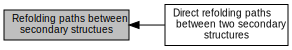
\includegraphics[width=350pt]{group__paths}
\end{center}
\end{figure}
\subsection*{Modules}
\begin{DoxyCompactItemize}
\item 
\hyperlink{group__direct__paths}{Direct refolding paths between two secondary structures}
\begin{DoxyCompactList}\small\item\em Implementation of heuristics to explore optimal (re-\/)folding paths between two secondary structures. \end{DoxyCompactList}\end{DoxyCompactItemize}


\subsection{Detailed Description}

\include{group__eval}
\include{group__loops}
\include{group__energy__parameters}
\include{group__model__details}
\include{group__data__structures}
\include{group__utils}
\hypertarget{group__mfe__fold}{}\section{Computing Minimum Free Energy (M\+F\+E) Structures}
\label{group__mfe__fold}\index{Computing Minimum Free Energy (\+M\+F\+E) Structures@{Computing Minimum Free Energy (\+M\+F\+E) Structures}}


This section covers all functions and variables related to the calculation of minimum free energy (M\+F\+E) structures.  


Collaboration diagram for Computing Minimum Free Energy (M\+F\+E) Structures\+:
\nopagebreak
\begin{figure}[H]
\begin{center}
\leavevmode
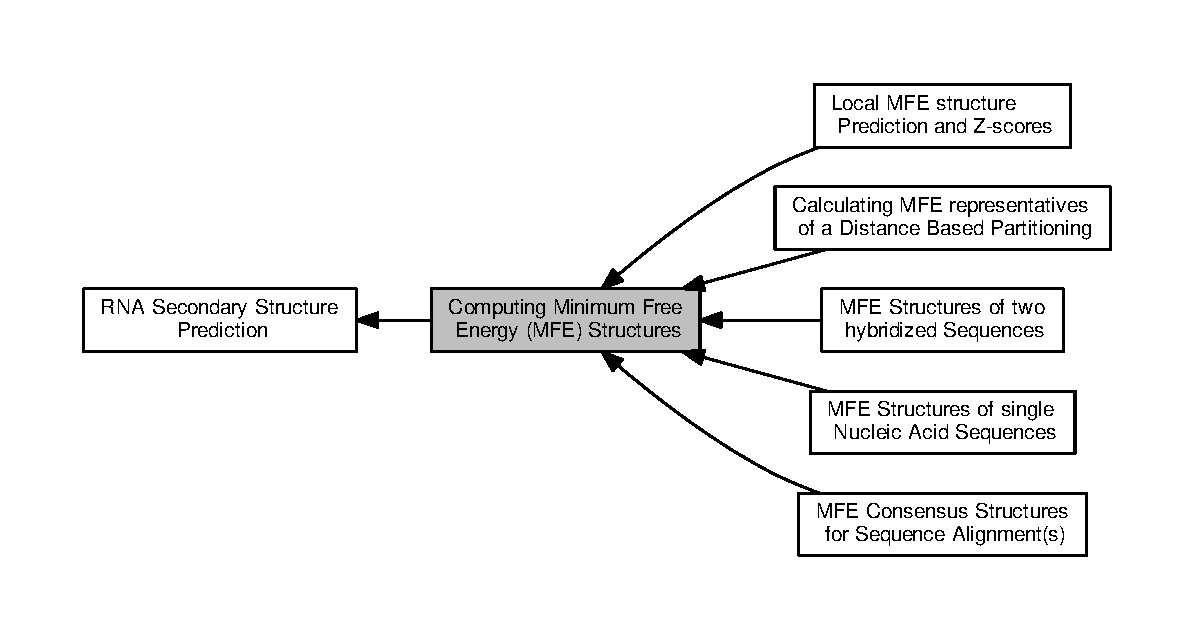
\includegraphics[width=350pt]{group__mfe__fold}
\end{center}
\end{figure}
\subsection*{Modules}
\begin{DoxyCompactItemize}
\item 
\hyperlink{group__mfe__fold__single}{M\+F\+E Structures of single Nucleic Acid Sequences}
\begin{DoxyCompactList}\small\item\em This module contains all functions and variables related to the calculation of global minimum free energy structures for single sequences. \end{DoxyCompactList}\item 
\hyperlink{group__mfe__cofold}{M\+F\+E Structures of two hybridized Sequences}
\item 
\hyperlink{group__consensus__mfe__fold}{M\+F\+E Consensus Structures for Sequence Alignment(s)}
\item 
\hyperlink{group__local__mfe__fold}{Local M\+F\+E structure Prediction and Z-\/scores}
\item 
\hyperlink{group__kl__neighborhood__mfe}{Calculating M\+F\+E representatives of a Distance Based Partitioning}
\begin{DoxyCompactList}\small\item\em Compute the minimum free energy (M\+F\+E) and secondary structures for a partitioning of the secondary structure space according to the base pair distance to two fixed reference structures basepair distance to two fixed reference structures. \end{DoxyCompactList}\end{DoxyCompactItemize}
\subsection*{Functions}
\begin{DoxyCompactItemize}
\item 
float \hyperlink{group__mfe__fold_gabd3b147371ccf25c577f88bbbaf159fd}{vrna\+\_\+mfe} (\hyperlink{group__fold__compound_ga1b0cef17fd40466cef5968eaeeff6166}{vrna\+\_\+fold\+\_\+compound\+\_\+t} $\ast$vc, char $\ast$structure)
\begin{DoxyCompactList}\small\item\em Compute minimum free energy and an appropriate secondary structure of an R\+N\+A sequence, or R\+N\+A sequence alignment. \end{DoxyCompactList}\end{DoxyCompactItemize}


\subsection{Detailed Description}
This section covers all functions and variables related to the calculation of minimum free energy (M\+F\+E) structures. 

The library provides a fast dynamic programming minimum free energy folding algorithm as described in \cite{zuker:1981}. All relevant parts that directly implement the \char`\"{}\+Zuker \& Stiegler\char`\"{} algorithm for single sequences are described in this section.

Folding of circular R\+N\+A sequences is handled as a post-\/processing step of the forward recursions. See \cite{hofacker:2006} for further details.

Nevertheless, the R\+N\+Alib also provides interfaces for the prediction of consensus M\+F\+E structures of sequence alignments, M\+F\+E structure for two hybridized sequences, local optimal structures and many more. For those more specialized variants of M\+F\+E folding routines, please consult the appropriate subsections (Modules) as listed above. 

\subsection{Function Documentation}
\hypertarget{group__mfe__fold_gabd3b147371ccf25c577f88bbbaf159fd}{}\index{Computing Minimum Free Energy (\+M\+F\+E) Structures@{Computing Minimum Free Energy (\+M\+F\+E) Structures}!vrna\+\_\+mfe@{vrna\+\_\+mfe}}
\index{vrna\+\_\+mfe@{vrna\+\_\+mfe}!Computing Minimum Free Energy (\+M\+F\+E) Structures@{Computing Minimum Free Energy (\+M\+F\+E) Structures}}
\subsubsection[{vrna\+\_\+mfe}]{\setlength{\rightskip}{0pt plus 5cm}float vrna\+\_\+mfe (
\begin{DoxyParamCaption}
\item[{{\bf vrna\+\_\+fold\+\_\+compound\+\_\+t} $\ast$}]{vc, }
\item[{char $\ast$}]{structure}
\end{DoxyParamCaption}
)}\label{group__mfe__fold_gabd3b147371ccf25c577f88bbbaf159fd}


{\ttfamily \#include $<$\hyperlink{mfe_8h}{Vienna\+R\+N\+A/mfe.\+h}$>$}



Compute minimum free energy and an appropriate secondary structure of an R\+N\+A sequence, or R\+N\+A sequence alignment. 

Depending on the type of the provided \hyperlink{group__fold__compound_ga1b0cef17fd40466cef5968eaeeff6166}{vrna\+\_\+fold\+\_\+compound\+\_\+t}, this function predicts the M\+F\+E for a single sequence, or a corresponding averaged M\+F\+E for a sequence alignment. If backtracking is activated, it also constructs the corresponding secondary structure, or consensus structure. Therefore, the second parameter, {\itshape structure}, has to point to an allocated block of memory with a size of at least $\mathrm{strlen}(\mathrm{sequence})+1$ to store the backtracked M\+F\+E structure. (For consensus structures, this is the length of the alignment + 1. If {\ttfamily N\+U\+L\+L} is passed, no backtracking will be performed.

\begin{DoxyNote}{Note}
This function is polymorphic. It accepts \hyperlink{group__fold__compound_ga1b0cef17fd40466cef5968eaeeff6166}{vrna\+\_\+fold\+\_\+compound\+\_\+t} of type \hyperlink{group__fold__compound_gga01a4ff86fa71deaaa5d1abbd95a1447da1608d3aa78905fc39e0d25a624ac9512}{V\+R\+N\+A\+\_\+\+V\+C\+\_\+\+T\+Y\+P\+E\+\_\+\+S\+I\+N\+G\+L\+E}, and \hyperlink{group__fold__compound_gga01a4ff86fa71deaaa5d1abbd95a1447da056345f1bcfe7cd595d1fd437c05246d}{V\+R\+N\+A\+\_\+\+V\+C\+\_\+\+T\+Y\+P\+E\+\_\+\+A\+L\+I\+G\+N\+M\+E\+N\+T}.
\end{DoxyNote}
\begin{DoxySeeAlso}{See also}
\hyperlink{group__fold__compound_ga1b0cef17fd40466cef5968eaeeff6166}{vrna\+\_\+fold\+\_\+compound\+\_\+t}, \hyperlink{group__fold__compound_ga6601d994ba32b11511b36f68b08403be}{vrna\+\_\+fold\+\_\+compound()}, \hyperlink{group__mfe__fold__single_gae7ca49ffb3086f145da36c964a7cec64}{vrna\+\_\+fold()}, \hyperlink{group__mfe__fold__single_gaa0f5bf321038f404b36a6147bdae4154}{vrna\+\_\+circfold()}, \hyperlink{group__fold__compound_gad6bacc816af274922b13d947f708aa0c}{vrna\+\_\+fold\+\_\+compound\+\_\+comparative()}, \hyperlink{group__consensus__mfe__fold_ga02098d0c8790f9a37fbef6ad0cfc705c}{vrna\+\_\+alifold()}, \hyperlink{group__consensus__mfe__fold_ga01ce2cff93ea44c4f4254760ca2bd16c}{vrna\+\_\+circalifold()}
\end{DoxySeeAlso}

\begin{DoxyParams}{Parameters}
{\em vc} & fold compound \\
\hline
{\em structure} & A pointer to the character array where the secondary structure in dot-\/bracket notation will be written to (Maybe N\+U\+L\+L)\\
\hline
\end{DoxyParams}
\begin{DoxyReturn}{Returns}
the minimum free energy (M\+F\+E) in kcal/mol 
\end{DoxyReturn}

\hypertarget{group__pf__fold}{\section{Computing Partition Functions and Pair Probabilities}
\label{group__pf__fold}\index{Computing Partition Functions and Pair Probabilities@{Computing Partition Functions and Pair Probabilities}}
}


This section provides information about all functions and variables related to the calculation of the partition function and base pair probabilities.  


Collaboration diagram for Computing Partition Functions and Pair Probabilities\+:
\nopagebreak
\begin{figure}[H]
\begin{center}
\leavevmode
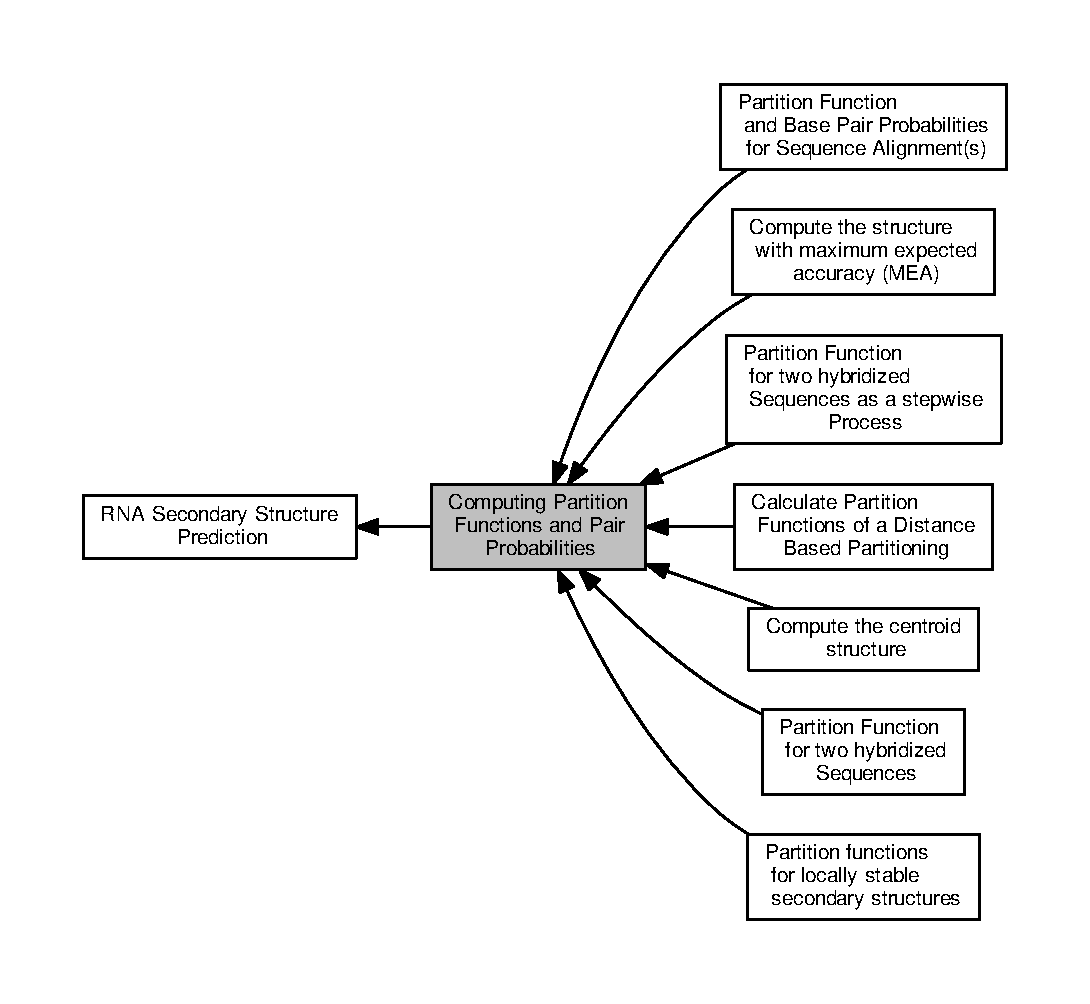
\includegraphics[width=350pt]{group__pf__fold}
\end{center}
\end{figure}
\subsection*{Modules}
\begin{DoxyCompactItemize}
\item 
\hyperlink{group__mea__fold}{Compute the structure with maximum expected accuracy (\+M\+E\+A)}
\item 
\hyperlink{group__centroid__fold}{Compute the centroid structure}
\item 
\hyperlink{group__pf__cofold}{Partition Function for two hybridized Sequences}
\begin{DoxyCompactList}\small\item\em Partition Function Cofolding. \end{DoxyCompactList}\item 
\hyperlink{group__up__cofold}{Partition Function for two hybridized Sequences as a stepwise Process}
\begin{DoxyCompactList}\small\item\em Partition Function Cofolding as a stepwise process. \end{DoxyCompactList}\item 
\hyperlink{group__consensus__pf__fold}{Partition Function and Base Pair Probabilities for Sequence Alignment(s)}
\item 
\hyperlink{group__local__pf__fold}{Partition functions for locally stable secondary structures}
\item 
\hyperlink{group__kl__neighborhood__pf}{Calculate Partition Functions of a Distance Based Partitioning}
\begin{DoxyCompactList}\small\item\em Compute the partition function and stochastically sample secondary structures for a partitioning of the secondary structure space according to the base pair distance to two fixed reference structures. \end{DoxyCompactList}\end{DoxyCompactItemize}
\subsection*{Files}
\begin{DoxyCompactItemize}
\item 
file \hyperlink{boltzmann__sampling_8h}{boltzmann\+\_\+sampling.\+h}
\begin{DoxyCompactList}\small\item\em Boltzmann Sampling of secondary structures from the ensemble. \end{DoxyCompactList}\item 
file \hyperlink{part__func_8h}{part\+\_\+func.\+h}
\begin{DoxyCompactList}\small\item\em Partition function of single R\+N\+A sequences. \end{DoxyCompactList}\end{DoxyCompactItemize}
\subsection*{Functions}
\begin{DoxyCompactItemize}
\item 
float \hyperlink{group__pf__fold_ga29e256d688ad221b78d37f427e0e99bc}{vrna\+\_\+pf} (\hyperlink{group__fold__compound_ga1b0cef17fd40466cef5968eaeeff6166}{vrna\+\_\+fold\+\_\+compound\+\_\+t} $\ast$vc, char $\ast$structure)
\begin{DoxyCompactList}\small\item\em Compute the partition function $Q$ for a given R\+N\+A sequence, or sequence alignment. \end{DoxyCompactList}\item 
float \hyperlink{group__pf__fold_ga59935ba485ac90f0efb5a38e2962d879}{vrna\+\_\+pf\+\_\+fold} (const char $\ast$seq, char $\ast$structure, \hyperlink{group__data__structures_ga8e4eb5e1bfc95776559575beb359af87}{vrna\+\_\+plist\+\_\+t} $\ast$$\ast$pl)
\begin{DoxyCompactList}\small\item\em Compute Partition function $Q$ (and base pair probabilities) for an R\+N\+A sequence using a comparative method. \end{DoxyCompactList}\item 
float \hyperlink{group__pf__fold_ga6dc133fce577fc0370986f3a3301cd10}{vrna\+\_\+pf\+\_\+circfold} (const char $\ast$seq, char $\ast$structure, \hyperlink{group__data__structures_ga8e4eb5e1bfc95776559575beb359af87}{vrna\+\_\+plist\+\_\+t} $\ast$$\ast$pl)
\begin{DoxyCompactList}\small\item\em Compute Partition function $Q$ (and base pair probabilities) for a circular R\+N\+A sequences using a comparative method. \end{DoxyCompactList}\item 
double \hyperlink{group__pf__fold_gad3f0c240512e6d43e2e4d4c2076021f5}{vrna\+\_\+mean\+\_\+bp\+\_\+distance\+\_\+pr} (int length, \hyperlink{group__data__structures_ga31125aeace516926bf7f251f759b6126}{F\+L\+T\+\_\+\+O\+R\+\_\+\+D\+B\+L} $\ast$\hyperlink{fold__vars_8h_ac98ec419070aee6831b44e5c700f090f}{pr})
\begin{DoxyCompactList}\small\item\em Get the mean base pair distance in the thermodynamic ensemble from a probability matrix. \end{DoxyCompactList}\item 
double \hyperlink{group__pf__fold_gaa6b8983b559b9ef4b2e1b31113ea317b}{vrna\+\_\+mean\+\_\+bp\+\_\+distance} (\hyperlink{group__fold__compound_ga1b0cef17fd40466cef5968eaeeff6166}{vrna\+\_\+fold\+\_\+compound\+\_\+t} $\ast$vc)
\begin{DoxyCompactList}\small\item\em Get the mean base pair distance in the thermodynamic ensemble. \end{DoxyCompactList}\item 
\hyperlink{group__data__structures_ga8e4eb5e1bfc95776559575beb359af87}{vrna\+\_\+plist\+\_\+t} $\ast$ \hyperlink{group__pf__fold_ga26e3cc2eb127a35625572e9275c24ee4}{vrna\+\_\+stack\+\_\+prob} (\hyperlink{group__fold__compound_ga1b0cef17fd40466cef5968eaeeff6166}{vrna\+\_\+fold\+\_\+compound\+\_\+t} $\ast$vc, double cutoff)
\begin{DoxyCompactList}\small\item\em Compute stacking probabilities. \end{DoxyCompactList}\item 
float \hyperlink{group__pf__fold_gac4f95bee734b2563a3d6e9932117ebdf}{pf\+\_\+fold\+\_\+par} (const char $\ast$sequence, char $\ast$structure, \hyperlink{group__energy__parameters_ga01d8b92fe734df8d79a6169482c7d8d8}{vrna\+\_\+exp\+\_\+param\+\_\+t} $\ast$parameters, int calculate\+\_\+bppm, int is\+\_\+constrained, int is\+\_\+circular)
\begin{DoxyCompactList}\small\item\em Compute the partition function $Q$ for a given R\+N\+A sequence. \end{DoxyCompactList}\item 
float \hyperlink{group__pf__fold_gadc3db3d98742427e7001a7fd36ef28c2}{pf\+\_\+fold} (const char $\ast$sequence, char $\ast$structure)
\begin{DoxyCompactList}\small\item\em Compute the partition function $Q$ of an R\+N\+A sequence. \end{DoxyCompactList}\item 
float \hyperlink{group__pf__fold_ga819ce5fca8984004ac81c4a3b04cb735}{pf\+\_\+circ\+\_\+fold} (const char $\ast$sequence, char $\ast$structure)
\begin{DoxyCompactList}\small\item\em Compute the partition function of a circular R\+N\+A sequence. \end{DoxyCompactList}\item 
void \hyperlink{group__pf__fold_gae73db3f49a94f0f72e067ecd12681dbd}{free\+\_\+pf\+\_\+arrays} (void)
\begin{DoxyCompactList}\small\item\em Free arrays for the partition function recursions. \end{DoxyCompactList}\item 
void \hyperlink{group__pf__fold_ga384e927890f9c034ff09fa66da102d28}{update\+\_\+pf\+\_\+params} (int length)
\begin{DoxyCompactList}\small\item\em Recalculate energy parameters. \end{DoxyCompactList}\item 
void \hyperlink{group__pf__fold_gaafe2d1b21f5418b123b088aa395e827d}{update\+\_\+pf\+\_\+params\+\_\+par} (int length, \hyperlink{group__energy__parameters_ga01d8b92fe734df8d79a6169482c7d8d8}{vrna\+\_\+exp\+\_\+param\+\_\+t} $\ast$parameters)
\begin{DoxyCompactList}\small\item\em Recalculate energy parameters. \end{DoxyCompactList}\item 
\hyperlink{group__data__structures_ga31125aeace516926bf7f251f759b6126}{F\+L\+T\+\_\+\+O\+R\+\_\+\+D\+B\+L} $\ast$ \hyperlink{group__pf__fold_gac5ac7ee281aae1c5cc5898a841178073}{export\+\_\+bppm} (void)
\begin{DoxyCompactList}\small\item\em Get a pointer to the base pair probability array

Accessing the base pair probabilities for a pair (i,j) is achieved by. \end{DoxyCompactList}\item 
int \hyperlink{group__pf__fold_ga42faebdfce6f070c5f89adfc8427525c}{get\+\_\+pf\+\_\+arrays} (short $\ast$$\ast$S\+\_\+p, short $\ast$$\ast$S1\+\_\+p, char $\ast$$\ast$ptype\+\_\+p, \hyperlink{group__data__structures_ga31125aeace516926bf7f251f759b6126}{F\+L\+T\+\_\+\+O\+R\+\_\+\+D\+B\+L} $\ast$$\ast$qb\+\_\+p, \hyperlink{group__data__structures_ga31125aeace516926bf7f251f759b6126}{F\+L\+T\+\_\+\+O\+R\+\_\+\+D\+B\+L} $\ast$$\ast$qm\+\_\+p, \hyperlink{group__data__structures_ga31125aeace516926bf7f251f759b6126}{F\+L\+T\+\_\+\+O\+R\+\_\+\+D\+B\+L} $\ast$$\ast$q1k\+\_\+p, \hyperlink{group__data__structures_ga31125aeace516926bf7f251f759b6126}{F\+L\+T\+\_\+\+O\+R\+\_\+\+D\+B\+L} $\ast$$\ast$qln\+\_\+p)
\begin{DoxyCompactList}\small\item\em Get the pointers to (almost) all relavant computation arrays used in partition function computation. \end{DoxyCompactList}\item 
double \hyperlink{group__pf__fold_ga79cbc375af65f11609feb6b055269e7d}{mean\+\_\+bp\+\_\+distance} (int length)
\begin{DoxyCompactList}\small\item\em Get the mean base pair distance of the last partition function computation. \end{DoxyCompactList}\item 
double \hyperlink{group__pf__fold_gad5ba36cef8d01cf4244cc09b9bf1ce1d}{mean\+\_\+bp\+\_\+distance\+\_\+pr} (int length, \hyperlink{group__data__structures_ga31125aeace516926bf7f251f759b6126}{F\+L\+T\+\_\+\+O\+R\+\_\+\+D\+B\+L} $\ast$\hyperlink{fold__vars_8h_ac98ec419070aee6831b44e5c700f090f}{pr})
\begin{DoxyCompactList}\small\item\em Get the mean base pair distance in the thermodynamic ensemble. \end{DoxyCompactList}\item 
\hyperlink{group__data__structures_ga8e4eb5e1bfc95776559575beb359af87}{vrna\+\_\+plist\+\_\+t} $\ast$ \hyperlink{group__pf__fold_gaa3bf26a0ee2e9f2225afbaee44a37264}{vrna\+\_\+plist\+\_\+from\+\_\+probs} (\hyperlink{group__fold__compound_ga1b0cef17fd40466cef5968eaeeff6166}{vrna\+\_\+fold\+\_\+compound\+\_\+t} $\ast$vc, double cut\+\_\+off)
\begin{DoxyCompactList}\small\item\em Create a \hyperlink{group__data__structures_ga8e4eb5e1bfc95776559575beb359af87}{vrna\+\_\+plist\+\_\+t} from base pair probability matrix. \end{DoxyCompactList}\item 
void \hyperlink{group__pf__fold_gacfdacc119b749bccf939de445afea07b}{assign\+\_\+plist\+\_\+from\+\_\+pr} (\hyperlink{group__data__structures_ga8e4eb5e1bfc95776559575beb359af87}{vrna\+\_\+plist\+\_\+t} $\ast$$\ast$pl, \hyperlink{group__data__structures_ga31125aeace516926bf7f251f759b6126}{F\+L\+T\+\_\+\+O\+R\+\_\+\+D\+B\+L} $\ast$probs, int length, double cutoff)
\begin{DoxyCompactList}\small\item\em Create a vrna\+\_\+plist\+\_\+t from a probability matrix. \end{DoxyCompactList}\end{DoxyCompactItemize}


\subsection{Detailed Description}
This section provides information about all functions and variables related to the calculation of the partition function and base pair probabilities. 

Instead of the minimum free energy structure the partition function of all possible structures and from that the pairing probability for every possible pair can be calculated, using a dynamic programming algorithm as described in {\bfseries [mccaskill\+:1990.]} 

\subsection{Function Documentation}
\hypertarget{group__pf__fold_ga29e256d688ad221b78d37f427e0e99bc}{\index{Computing Partition Functions and Pair Probabilities@{Computing Partition Functions and Pair Probabilities}!vrna\+\_\+pf@{vrna\+\_\+pf}}
\index{vrna\+\_\+pf@{vrna\+\_\+pf}!Computing Partition Functions and Pair Probabilities@{Computing Partition Functions and Pair Probabilities}}
\subsubsection[{vrna\+\_\+pf}]{\setlength{\rightskip}{0pt plus 5cm}float vrna\+\_\+pf (
\begin{DoxyParamCaption}
\item[{{\bf vrna\+\_\+fold\+\_\+compound\+\_\+t} $\ast$}]{vc, }
\item[{char $\ast$}]{structure}
\end{DoxyParamCaption}
)}}\label{group__pf__fold_ga29e256d688ad221b78d37f427e0e99bc}


{\ttfamily \#include $<$\hyperlink{part__func_8h}{Vienna\+R\+N\+A/part\+\_\+func.\+h}$>$}



Compute the partition function $Q$ for a given R\+N\+A sequence, or sequence alignment. 

If {\itshape structure} is not a N\+U\+L\+L pointer on input, it contains on return a string consisting of the letters \char`\"{} . , $\vert$ \{ \} ( ) \char`\"{} denoting bases that are essentially unpaired, weakly paired, strongly paired without preference, weakly upstream (downstream) paired, or strongly up-\/ (down-\/)stream paired bases, respectively. If the parameter calculate\+\_\+bppm is set to 0 base pairing probabilities will not be computed (saving C\+P\+U time), otherwise after calculations took place \hyperlink{fold__vars_8h_ac98ec419070aee6831b44e5c700f090f}{pr} will contain the probability that bases {\itshape i} and {\itshape j} pair.

\begin{DoxyNote}{Note}
This function is polymorphic. It accepts \hyperlink{group__fold__compound_ga1b0cef17fd40466cef5968eaeeff6166}{vrna\+\_\+fold\+\_\+compound\+\_\+t} of type \hyperlink{group__fold__compound_gga01a4ff86fa71deaaa5d1abbd95a1447da1608d3aa78905fc39e0d25a624ac9512}{V\+R\+N\+A\+\_\+\+V\+C\+\_\+\+T\+Y\+P\+E\+\_\+\+S\+I\+N\+G\+L\+E}, and \hyperlink{group__fold__compound_gga01a4ff86fa71deaaa5d1abbd95a1447da056345f1bcfe7cd595d1fd437c05246d}{V\+R\+N\+A\+\_\+\+V\+C\+\_\+\+T\+Y\+P\+E\+\_\+\+A\+L\+I\+G\+N\+M\+E\+N\+T}.
\end{DoxyNote}
\begin{DoxySeeAlso}{See also}
\hyperlink{group__fold__compound_ga1b0cef17fd40466cef5968eaeeff6166}{vrna\+\_\+fold\+\_\+compound\+\_\+t}, \hyperlink{group__fold__compound_ga6601d994ba32b11511b36f68b08403be}{vrna\+\_\+fold\+\_\+compound()}, \hyperlink{group__pf__fold_ga59935ba485ac90f0efb5a38e2962d879}{vrna\+\_\+pf\+\_\+fold()}, \hyperlink{group__pf__fold_ga6dc133fce577fc0370986f3a3301cd10}{vrna\+\_\+pf\+\_\+circfold()}, \hyperlink{group__fold__compound_gad6bacc816af274922b13d947f708aa0c}{vrna\+\_\+fold\+\_\+compound\+\_\+comparative()}, \hyperlink{group__consensus__pf__fold_gaef750636c70e597a85ee139197a4350d}{vrna\+\_\+pf\+\_\+alifold()}, \hyperlink{group__consensus__pf__fold_ga017209394a4c1e68d96cd47e61d16d25}{vrna\+\_\+pf\+\_\+circalifold()}, \hyperlink{group__struct__utils_ga0c28c410a5ab22d6ab9c77a84e8d5b44}{vrna\+\_\+db\+\_\+from\+\_\+probs()}, \hyperlink{group__energy__parameters_gab1f3016f96aa96bff020cdd904605afa}{vrna\+\_\+exp\+\_\+params()}, \hyperlink{group__aln__utils_gaf6421a1318586c59fea6a127ed9f65f3}{vrna\+\_\+aln\+\_\+pinfo()}
\end{DoxySeeAlso}

\begin{DoxyParams}[1]{Parameters}
\mbox{\tt in,out}  & {\em vc} & The fold compound data structure \\
\hline
\mbox{\tt in,out}  & {\em structure} & A pointer to the character array where position-\/wise pairing propensity will be stored. (Maybe N\+U\+L\+L) \\
\hline
\end{DoxyParams}
\begin{DoxyReturn}{Returns}
The Gibbs free energy of the ensemble ( $G = -RT \cdot \log(Q) $) in kcal/mol 
\end{DoxyReturn}
\hypertarget{group__pf__fold_ga59935ba485ac90f0efb5a38e2962d879}{\index{Computing Partition Functions and Pair Probabilities@{Computing Partition Functions and Pair Probabilities}!vrna\+\_\+pf\+\_\+fold@{vrna\+\_\+pf\+\_\+fold}}
\index{vrna\+\_\+pf\+\_\+fold@{vrna\+\_\+pf\+\_\+fold}!Computing Partition Functions and Pair Probabilities@{Computing Partition Functions and Pair Probabilities}}
\subsubsection[{vrna\+\_\+pf\+\_\+fold}]{\setlength{\rightskip}{0pt plus 5cm}float vrna\+\_\+pf\+\_\+fold (
\begin{DoxyParamCaption}
\item[{const char $\ast$}]{seq, }
\item[{char $\ast$}]{structure, }
\item[{{\bf vrna\+\_\+plist\+\_\+t} $\ast$$\ast$}]{pl}
\end{DoxyParamCaption}
)}}\label{group__pf__fold_ga59935ba485ac90f0efb5a38e2962d879}


{\ttfamily \#include $<$\hyperlink{part__func_8h}{Vienna\+R\+N\+A/part\+\_\+func.\+h}$>$}



Compute Partition function $Q$ (and base pair probabilities) for an R\+N\+A sequence using a comparative method. 

This simplified interface to \hyperlink{group__pf__fold_ga29e256d688ad221b78d37f427e0e99bc}{vrna\+\_\+pf()} computes the partition function and, if required, base pair probabilities for an R\+N\+A sequence using default options. Memory required for dynamic programming (D\+P) matrices will be allocated and free'd on-\/the-\/fly. Hence, after return of this function, the recursively filled matrices are not available any more for any post-\/processing.

\begin{DoxyNote}{Note}
In case you want to use the filled D\+P matrices for any subsequent post-\/processing step, or you require other conditions than specified by the default model details, use \hyperlink{group__pf__fold_ga29e256d688ad221b78d37f427e0e99bc}{vrna\+\_\+pf()}, and the data structure \hyperlink{group__fold__compound_ga1b0cef17fd40466cef5968eaeeff6166}{vrna\+\_\+fold\+\_\+compound\+\_\+t} instead.
\end{DoxyNote}
\begin{DoxySeeAlso}{See also}
\hyperlink{group__pf__fold_ga6dc133fce577fc0370986f3a3301cd10}{vrna\+\_\+pf\+\_\+circfold()}, \hyperlink{group__pf__fold_ga29e256d688ad221b78d37f427e0e99bc}{vrna\+\_\+pf()}, \hyperlink{group__fold__compound_ga6601d994ba32b11511b36f68b08403be}{vrna\+\_\+fold\+\_\+compound()}, \hyperlink{group__fold__compound_ga1b0cef17fd40466cef5968eaeeff6166}{vrna\+\_\+fold\+\_\+compound\+\_\+t}
\end{DoxySeeAlso}

\begin{DoxyParams}{Parameters}
{\em sequences} & R\+N\+A sequence \\
\hline
{\em structure} & A pointer to the character array where position-\/wise pairing propensity will be stored. (Maybe N\+U\+L\+L) \\
\hline
{\em pl} & A pointer to a list of \hyperlink{group__data__structures_ga8e4eb5e1bfc95776559575beb359af87}{vrna\+\_\+plist\+\_\+t} to store pairing probabilities (Maybe N\+U\+L\+L) \\
\hline
\end{DoxyParams}
\begin{DoxyReturn}{Returns}
The Gibbs free energy of the ensemble ( $G = -RT \cdot \log(Q) $) in kcal/mol 
\end{DoxyReturn}
\hypertarget{group__pf__fold_ga6dc133fce577fc0370986f3a3301cd10}{\index{Computing Partition Functions and Pair Probabilities@{Computing Partition Functions and Pair Probabilities}!vrna\+\_\+pf\+\_\+circfold@{vrna\+\_\+pf\+\_\+circfold}}
\index{vrna\+\_\+pf\+\_\+circfold@{vrna\+\_\+pf\+\_\+circfold}!Computing Partition Functions and Pair Probabilities@{Computing Partition Functions and Pair Probabilities}}
\subsubsection[{vrna\+\_\+pf\+\_\+circfold}]{\setlength{\rightskip}{0pt plus 5cm}float vrna\+\_\+pf\+\_\+circfold (
\begin{DoxyParamCaption}
\item[{const char $\ast$}]{seq, }
\item[{char $\ast$}]{structure, }
\item[{{\bf vrna\+\_\+plist\+\_\+t} $\ast$$\ast$}]{pl}
\end{DoxyParamCaption}
)}}\label{group__pf__fold_ga6dc133fce577fc0370986f3a3301cd10}


{\ttfamily \#include $<$\hyperlink{part__func_8h}{Vienna\+R\+N\+A/part\+\_\+func.\+h}$>$}



Compute Partition function $Q$ (and base pair probabilities) for a circular R\+N\+A sequences using a comparative method. 

This simplified interface to \hyperlink{group__pf__fold_ga29e256d688ad221b78d37f427e0e99bc}{vrna\+\_\+pf()} computes the partition function and, if required, base pair probabilities for a circular R\+N\+A sequence using default options. Memory required for dynamic programming (D\+P) matrices will be allocated and free'd on-\/the-\/fly. Hence, after return of this function, the recursively filled matrices are not available any more for any post-\/processing.

\begin{DoxyNote}{Note}
In case you want to use the filled D\+P matrices for any subsequent post-\/processing step, or you require other conditions than specified by the default model details, use \hyperlink{group__pf__fold_ga29e256d688ad221b78d37f427e0e99bc}{vrna\+\_\+pf()}, and the data structure \hyperlink{group__fold__compound_ga1b0cef17fd40466cef5968eaeeff6166}{vrna\+\_\+fold\+\_\+compound\+\_\+t} instead.
\end{DoxyNote}
Folding of circular R\+N\+A sequences is handled as a post-\/processing step of the forward recursions. See \cite{hofacker:2006} for further details.

\begin{DoxySeeAlso}{See also}
\hyperlink{group__pf__fold_ga59935ba485ac90f0efb5a38e2962d879}{vrna\+\_\+pf\+\_\+fold()}, \hyperlink{group__pf__fold_ga29e256d688ad221b78d37f427e0e99bc}{vrna\+\_\+pf()}, \hyperlink{group__fold__compound_ga6601d994ba32b11511b36f68b08403be}{vrna\+\_\+fold\+\_\+compound()}, \hyperlink{group__fold__compound_ga1b0cef17fd40466cef5968eaeeff6166}{vrna\+\_\+fold\+\_\+compound\+\_\+t}
\end{DoxySeeAlso}

\begin{DoxyParams}{Parameters}
{\em sequences} & A circular R\+N\+A sequence \\
\hline
{\em structure} & A pointer to the character array where position-\/wise pairing propensity will be stored. (Maybe N\+U\+L\+L) \\
\hline
{\em pl} & A pointer to a list of \hyperlink{group__data__structures_ga8e4eb5e1bfc95776559575beb359af87}{vrna\+\_\+plist\+\_\+t} to store pairing probabilities (Maybe N\+U\+L\+L) \\
\hline
\end{DoxyParams}
\begin{DoxyReturn}{Returns}
The Gibbs free energy of the ensemble ( $G = -RT \cdot \log(Q) $) in kcal/mol 
\end{DoxyReturn}
\hypertarget{group__pf__fold_gad3f0c240512e6d43e2e4d4c2076021f5}{\index{Computing Partition Functions and Pair Probabilities@{Computing Partition Functions and Pair Probabilities}!vrna\+\_\+mean\+\_\+bp\+\_\+distance\+\_\+pr@{vrna\+\_\+mean\+\_\+bp\+\_\+distance\+\_\+pr}}
\index{vrna\+\_\+mean\+\_\+bp\+\_\+distance\+\_\+pr@{vrna\+\_\+mean\+\_\+bp\+\_\+distance\+\_\+pr}!Computing Partition Functions and Pair Probabilities@{Computing Partition Functions and Pair Probabilities}}
\subsubsection[{vrna\+\_\+mean\+\_\+bp\+\_\+distance\+\_\+pr}]{\setlength{\rightskip}{0pt plus 5cm}double vrna\+\_\+mean\+\_\+bp\+\_\+distance\+\_\+pr (
\begin{DoxyParamCaption}
\item[{int}]{length, }
\item[{{\bf F\+L\+T\+\_\+\+O\+R\+\_\+\+D\+B\+L} $\ast$}]{pr}
\end{DoxyParamCaption}
)}}\label{group__pf__fold_gad3f0c240512e6d43e2e4d4c2076021f5}


{\ttfamily \#include $<$\hyperlink{part__func_8h}{Vienna\+R\+N\+A/part\+\_\+func.\+h}$>$}



Get the mean base pair distance in the thermodynamic ensemble from a probability matrix. 

$<d> = \sum_{a,b} p_a p_b d(S_a,S_b)$~\newline
this can be computed from the pair probs $p_ij$ as~\newline
 $<d> = \sum_{ij} p_{ij}(1-p_{ij})$


\begin{DoxyParams}{Parameters}
{\em length} & The length of the sequence \\
\hline
{\em pr} & The matrix containing the base pair probabilities \\
\hline
\end{DoxyParams}
\begin{DoxyReturn}{Returns}
The mean pair distance of the structure ensemble 
\end{DoxyReturn}
\hypertarget{group__pf__fold_gaa6b8983b559b9ef4b2e1b31113ea317b}{\index{Computing Partition Functions and Pair Probabilities@{Computing Partition Functions and Pair Probabilities}!vrna\+\_\+mean\+\_\+bp\+\_\+distance@{vrna\+\_\+mean\+\_\+bp\+\_\+distance}}
\index{vrna\+\_\+mean\+\_\+bp\+\_\+distance@{vrna\+\_\+mean\+\_\+bp\+\_\+distance}!Computing Partition Functions and Pair Probabilities@{Computing Partition Functions and Pair Probabilities}}
\subsubsection[{vrna\+\_\+mean\+\_\+bp\+\_\+distance}]{\setlength{\rightskip}{0pt plus 5cm}double vrna\+\_\+mean\+\_\+bp\+\_\+distance (
\begin{DoxyParamCaption}
\item[{{\bf vrna\+\_\+fold\+\_\+compound\+\_\+t} $\ast$}]{vc}
\end{DoxyParamCaption}
)}}\label{group__pf__fold_gaa6b8983b559b9ef4b2e1b31113ea317b}


{\ttfamily \#include $<$\hyperlink{part__func_8h}{Vienna\+R\+N\+A/part\+\_\+func.\+h}$>$}



Get the mean base pair distance in the thermodynamic ensemble. 

$<d> = \sum_{a,b} p_a p_b d(S_a,S_b)$~\newline
this can be computed from the pair probs $p_ij$ as~\newline
 $<d> = \sum_{ij} p_{ij}(1-p_{ij})$


\begin{DoxyParams}{Parameters}
{\em vc} & The fold compound data structure \\
\hline
\end{DoxyParams}
\begin{DoxyReturn}{Returns}
The mean pair distance of the structure ensemble 
\end{DoxyReturn}
\hypertarget{group__pf__fold_ga26e3cc2eb127a35625572e9275c24ee4}{\index{Computing Partition Functions and Pair Probabilities@{Computing Partition Functions and Pair Probabilities}!vrna\+\_\+stack\+\_\+prob@{vrna\+\_\+stack\+\_\+prob}}
\index{vrna\+\_\+stack\+\_\+prob@{vrna\+\_\+stack\+\_\+prob}!Computing Partition Functions and Pair Probabilities@{Computing Partition Functions and Pair Probabilities}}
\subsubsection[{vrna\+\_\+stack\+\_\+prob}]{\setlength{\rightskip}{0pt plus 5cm}{\bf vrna\+\_\+plist\+\_\+t}$\ast$ vrna\+\_\+stack\+\_\+prob (
\begin{DoxyParamCaption}
\item[{{\bf vrna\+\_\+fold\+\_\+compound\+\_\+t} $\ast$}]{vc, }
\item[{double}]{cutoff}
\end{DoxyParamCaption}
)}}\label{group__pf__fold_ga26e3cc2eb127a35625572e9275c24ee4}


{\ttfamily \#include $<$\hyperlink{part__func_8h}{Vienna\+R\+N\+A/part\+\_\+func.\+h}$>$}



Compute stacking probabilities. 

For each possible base pair $(i,j)$, compute the probability of a stack $(i,j)$, $(i+1, j-1)$.


\begin{DoxyParams}{Parameters}
{\em vc} & The fold compound data structure with precomputed base pair probabilities \\
\hline
{\em cutoff} & A cutoff value that limits the output to stacks with $ p > \textrm{cutoff} $. \\
\hline
\end{DoxyParams}
\begin{DoxyReturn}{Returns}
A list of stacks with enclosing base pair $(i,j)$ and probabiltiy $ p $ 
\end{DoxyReturn}
\hypertarget{group__pf__fold_gac4f95bee734b2563a3d6e9932117ebdf}{\index{Computing Partition Functions and Pair Probabilities@{Computing Partition Functions and Pair Probabilities}!pf\+\_\+fold\+\_\+par@{pf\+\_\+fold\+\_\+par}}
\index{pf\+\_\+fold\+\_\+par@{pf\+\_\+fold\+\_\+par}!Computing Partition Functions and Pair Probabilities@{Computing Partition Functions and Pair Probabilities}}
\subsubsection[{pf\+\_\+fold\+\_\+par}]{\setlength{\rightskip}{0pt plus 5cm}float pf\+\_\+fold\+\_\+par (
\begin{DoxyParamCaption}
\item[{const char $\ast$}]{sequence, }
\item[{char $\ast$}]{structure, }
\item[{{\bf vrna\+\_\+exp\+\_\+param\+\_\+t} $\ast$}]{parameters, }
\item[{int}]{calculate\+\_\+bppm, }
\item[{int}]{is\+\_\+constrained, }
\item[{int}]{is\+\_\+circular}
\end{DoxyParamCaption}
)}}\label{group__pf__fold_gac4f95bee734b2563a3d6e9932117ebdf}


{\ttfamily \#include $<$\hyperlink{part__func_8h}{Vienna\+R\+N\+A/part\+\_\+func.\+h}$>$}



Compute the partition function $Q$ for a given R\+N\+A sequence. 

If {\itshape structure} is not a N\+U\+L\+L pointer on input, it contains on return a string consisting of the letters \char`\"{} . , $\vert$ \{ \} ( ) \char`\"{} denoting bases that are essentially unpaired, weakly paired, strongly paired without preference, weakly upstream (downstream) paired, or strongly up-\/ (down-\/)stream paired bases, respectively. If \hyperlink{fold__vars_8h_a0afc287c2464866d94858c39175154af}{fold\+\_\+constrained} is not 0, the {\itshape structure} string is interpreted on input as a list of constraints for the folding. The character \char`\"{}x\char`\"{} marks bases that must be unpaired, matching brackets \char`\"{} ( ) \char`\"{} denote base pairs, all other characters are ignored. Any pairs conflicting with the constraint will be forbidden. This is usually sufficient to ensure the constraints are honored. If the parameter calculate\+\_\+bppm is set to 0 base pairing probabilities will not be computed (saving C\+P\+U time), otherwise after calculations took place \hyperlink{fold__vars_8h_ac98ec419070aee6831b44e5c700f090f}{pr} will contain the probability that bases {\itshape i} and {\itshape j} pair.

\begin{DoxyRefDesc}{Deprecated}
\item[\hyperlink{deprecated__deprecated000094}{Deprecated}]Use \hyperlink{group__pf__fold_ga29e256d688ad221b78d37f427e0e99bc}{vrna\+\_\+pf()} instead\end{DoxyRefDesc}


\begin{DoxyNote}{Note}
The global array \hyperlink{fold__vars_8h_ac98ec419070aee6831b44e5c700f090f}{pr} is deprecated and the user who wants the calculated base pair probabilities for further computations is advised to use the function \hyperlink{group__pf__fold_gac5ac7ee281aae1c5cc5898a841178073}{export\+\_\+bppm()} 
\end{DoxyNote}
\begin{DoxyPostcond}{Postcondition}
After successful run the hidden folding matrices are filled with the appropriate Boltzmann factors. Depending on whether the global variable \hyperlink{group__model__details_gad512b5dd4dbec60faccfe137bb474489}{do\+\_\+backtrack} was set the base pair probabilities are already computed and may be accessed for further usage via the \hyperlink{group__pf__fold_gac5ac7ee281aae1c5cc5898a841178073}{export\+\_\+bppm()} function. A call of \hyperlink{group__pf__fold_gae73db3f49a94f0f72e067ecd12681dbd}{free\+\_\+pf\+\_\+arrays()} will free all memory allocated by this function. Successive calls will first free previously allocated memory before starting the computation. 
\end{DoxyPostcond}
\begin{DoxySeeAlso}{See also}
\hyperlink{group__pf__fold_ga29e256d688ad221b78d37f427e0e99bc}{vrna\+\_\+pf()}, \hyperlink{group__struct__utils_ga129d81c4a1ead793c5b2311333e03dfa}{bppm\+\_\+to\+\_\+structure()}, \hyperlink{group__pf__fold_gac5ac7ee281aae1c5cc5898a841178073}{export\+\_\+bppm()}, \hyperlink{group__energy__parameters_gab1f3016f96aa96bff020cdd904605afa}{vrna\+\_\+exp\+\_\+params()}, \hyperlink{group__pf__fold_gae73db3f49a94f0f72e067ecd12681dbd}{free\+\_\+pf\+\_\+arrays()} 
\end{DoxySeeAlso}

\begin{DoxyParams}[1]{Parameters}
\mbox{\tt in}  & {\em sequence} & The R\+N\+A sequence input \\
\hline
\mbox{\tt in,out}  & {\em structure} & A pointer to a char array where a base pair probability information can be stored in a pseudo-\/dot-\/bracket notation (may be N\+U\+L\+L, too) \\
\hline
\mbox{\tt in}  & {\em parameters} & Data structure containing the precalculated Boltzmann factors \\
\hline
\mbox{\tt in}  & {\em calculate\+\_\+bppm} & Switch to Base pair probability calculations on/off (0==off) \\
\hline
\mbox{\tt in}  & {\em is\+\_\+constrained} & Switch to indicate that a structure contraint is passed via the structure argument (0==off) \\
\hline
\mbox{\tt in}  & {\em is\+\_\+circular} & Switch to (de-\/)activate postprocessing steps in case R\+N\+A sequence is circular (0==off) \\
\hline
\end{DoxyParams}
\begin{DoxyReturn}{Returns}
The Gibbs free energy of the ensemble ( $G = -RT \cdot \log(Q) $) in kcal/mol 
\end{DoxyReturn}
\hypertarget{group__pf__fold_gadc3db3d98742427e7001a7fd36ef28c2}{\index{Computing Partition Functions and Pair Probabilities@{Computing Partition Functions and Pair Probabilities}!pf\+\_\+fold@{pf\+\_\+fold}}
\index{pf\+\_\+fold@{pf\+\_\+fold}!Computing Partition Functions and Pair Probabilities@{Computing Partition Functions and Pair Probabilities}}
\subsubsection[{pf\+\_\+fold}]{\setlength{\rightskip}{0pt plus 5cm}float pf\+\_\+fold (
\begin{DoxyParamCaption}
\item[{const char $\ast$}]{sequence, }
\item[{char $\ast$}]{structure}
\end{DoxyParamCaption}
)}}\label{group__pf__fold_gadc3db3d98742427e7001a7fd36ef28c2}


{\ttfamily \#include $<$\hyperlink{part__func_8h}{Vienna\+R\+N\+A/part\+\_\+func.\+h}$>$}



Compute the partition function $Q$ of an R\+N\+A sequence. 

If {\itshape structure} is not a N\+U\+L\+L pointer on input, it contains on return a string consisting of the letters \char`\"{} . , $\vert$ \{ \} ( ) \char`\"{} denoting bases that are essentially unpaired, weakly paired, strongly paired without preference, weakly upstream (downstream) paired, or strongly up-\/ (down-\/)stream paired bases, respectively. If \hyperlink{fold__vars_8h_a0afc287c2464866d94858c39175154af}{fold\+\_\+constrained} is not 0, the {\itshape structure} string is interpreted on input as a list of constraints for the folding. The character \char`\"{}x\char`\"{} marks bases that must be unpaired, matching brackets \char`\"{} ( ) \char`\"{} denote base pairs, all other characters are ignored. Any pairs conflicting with the constraint will be forbidden. This is usually sufficient to ensure the constraints are honored. If \hyperlink{group__model__details_gad512b5dd4dbec60faccfe137bb474489}{do\+\_\+backtrack} has been set to 0 base pairing probabilities will not be computed (saving C\+P\+U time), otherwise \hyperlink{fold__vars_8h_ac98ec419070aee6831b44e5c700f090f}{pr} will contain the probability that bases {\itshape i} and {\itshape j} pair.

\begin{DoxyNote}{Note}
The global array \hyperlink{fold__vars_8h_ac98ec419070aee6831b44e5c700f090f}{pr} is deprecated and the user who wants the calculated base pair probabilities for further computations is advised to use the function \hyperlink{group__pf__fold_gac5ac7ee281aae1c5cc5898a841178073}{export\+\_\+bppm()}. 

{\bfseries Open\+M\+P\+:} This function is not entirely threadsafe. While the recursions are working on their own copies of data the model details for the recursions are determined from the global settings just before entering the recursions. Consider using \hyperlink{group__pf__fold_gac4f95bee734b2563a3d6e9932117ebdf}{pf\+\_\+fold\+\_\+par()} for a really threadsafe implementation. 
\end{DoxyNote}
\begin{DoxyPrecond}{Precondition}
This function takes its model details from the global variables provided in {\itshape R\+N\+Alib} 
\end{DoxyPrecond}
\begin{DoxyPostcond}{Postcondition}
After successful run the hidden folding matrices are filled with the appropriate Boltzmann factors. Depending on whether the global variable \hyperlink{group__model__details_gad512b5dd4dbec60faccfe137bb474489}{do\+\_\+backtrack} was set the base pair probabilities are already computed and may be accessed for further usage via the \hyperlink{group__pf__fold_gac5ac7ee281aae1c5cc5898a841178073}{export\+\_\+bppm()} function. A call of \hyperlink{group__pf__fold_gae73db3f49a94f0f72e067ecd12681dbd}{free\+\_\+pf\+\_\+arrays()} will free all memory allocated by this function. Successive calls will first free previously allocated memory before starting the computation. 
\end{DoxyPostcond}
\begin{DoxySeeAlso}{See also}
\hyperlink{group__pf__fold_gac4f95bee734b2563a3d6e9932117ebdf}{pf\+\_\+fold\+\_\+par()}, \hyperlink{group__pf__fold_ga819ce5fca8984004ac81c4a3b04cb735}{pf\+\_\+circ\+\_\+fold()}, \hyperlink{group__struct__utils_ga129d81c4a1ead793c5b2311333e03dfa}{bppm\+\_\+to\+\_\+structure()}, \hyperlink{group__pf__fold_gac5ac7ee281aae1c5cc5898a841178073}{export\+\_\+bppm()} 
\end{DoxySeeAlso}

\begin{DoxyParams}{Parameters}
{\em sequence} & The R\+N\+A sequence input \\
\hline
{\em structure} & A pointer to a char array where a base pair probability information can be stored in a pseudo-\/dot-\/bracket notation (may be N\+U\+L\+L, too) \\
\hline
\end{DoxyParams}
\begin{DoxyReturn}{Returns}
The Gibbs free energy of the ensemble ( $G = -RT \cdot \log(Q) $) in kcal/mol 
\end{DoxyReturn}
\hypertarget{group__pf__fold_ga819ce5fca8984004ac81c4a3b04cb735}{\index{Computing Partition Functions and Pair Probabilities@{Computing Partition Functions and Pair Probabilities}!pf\+\_\+circ\+\_\+fold@{pf\+\_\+circ\+\_\+fold}}
\index{pf\+\_\+circ\+\_\+fold@{pf\+\_\+circ\+\_\+fold}!Computing Partition Functions and Pair Probabilities@{Computing Partition Functions and Pair Probabilities}}
\subsubsection[{pf\+\_\+circ\+\_\+fold}]{\setlength{\rightskip}{0pt plus 5cm}float pf\+\_\+circ\+\_\+fold (
\begin{DoxyParamCaption}
\item[{const char $\ast$}]{sequence, }
\item[{char $\ast$}]{structure}
\end{DoxyParamCaption}
)}}\label{group__pf__fold_ga819ce5fca8984004ac81c4a3b04cb735}


{\ttfamily \#include $<$\hyperlink{part__func_8h}{Vienna\+R\+N\+A/part\+\_\+func.\+h}$>$}



Compute the partition function of a circular R\+N\+A sequence. 

\begin{DoxyNote}{Note}
The global array \hyperlink{fold__vars_8h_ac98ec419070aee6831b44e5c700f090f}{pr} is deprecated and the user who wants the calculated base pair probabilities for further computations is advised to use the function \hyperlink{group__pf__fold_gac5ac7ee281aae1c5cc5898a841178073}{export\+\_\+bppm()}. 

{\bfseries Open\+M\+P\+:} This function is not entirely threadsafe. While the recursions are working on their own copies of data the model details for the recursions are determined from the global settings just before entering the recursions. Consider using \hyperlink{group__pf__fold_gac4f95bee734b2563a3d6e9932117ebdf}{pf\+\_\+fold\+\_\+par()} for a really threadsafe implementation. 
\end{DoxyNote}
\begin{DoxyPrecond}{Precondition}
This function takes its model details from the global variables provided in {\itshape R\+N\+Alib} 
\end{DoxyPrecond}
\begin{DoxyPostcond}{Postcondition}
After successful run the hidden folding matrices are filled with the appropriate Boltzmann factors. Depending on whether the global variable \hyperlink{group__model__details_gad512b5dd4dbec60faccfe137bb474489}{do\+\_\+backtrack} was set the base pair probabilities are already computed and may be accessed for further usage via the \hyperlink{group__pf__fold_gac5ac7ee281aae1c5cc5898a841178073}{export\+\_\+bppm()} function. A call of \hyperlink{group__pf__fold_gae73db3f49a94f0f72e067ecd12681dbd}{free\+\_\+pf\+\_\+arrays()} will free all memory allocated by this function. Successive calls will first free previously allocated memory before starting the computation. 
\end{DoxyPostcond}
\begin{DoxySeeAlso}{See also}
\hyperlink{group__pf__fold_ga29e256d688ad221b78d37f427e0e99bc}{vrna\+\_\+pf()} 
\end{DoxySeeAlso}
\begin{DoxyRefDesc}{Deprecated}
\item[\hyperlink{deprecated__deprecated000095}{Deprecated}]Use \hyperlink{group__pf__fold_ga29e256d688ad221b78d37f427e0e99bc}{vrna\+\_\+pf()} instead! 
\begin{DoxyParams}[1]{Parameters}
\mbox{\tt in}  & {\em sequence} & The R\+N\+A sequence input \\
\hline
\mbox{\tt in,out}  & {\em structure} & A pointer to a char array where a base pair probability information can be stored in a pseudo-\/dot-\/bracket notation (may be N\+U\+L\+L, too) \\
\hline
\end{DoxyParams}
\begin{DoxyReturn}{Returns}
The Gibbs free energy of the ensemble ( $G = -RT \cdot \log(Q) $) in kcal/mol 
\end{DoxyReturn}
\end{DoxyRefDesc}
\hypertarget{group__pf__fold_gae73db3f49a94f0f72e067ecd12681dbd}{\index{Computing Partition Functions and Pair Probabilities@{Computing Partition Functions and Pair Probabilities}!free\+\_\+pf\+\_\+arrays@{free\+\_\+pf\+\_\+arrays}}
\index{free\+\_\+pf\+\_\+arrays@{free\+\_\+pf\+\_\+arrays}!Computing Partition Functions and Pair Probabilities@{Computing Partition Functions and Pair Probabilities}}
\subsubsection[{free\+\_\+pf\+\_\+arrays}]{\setlength{\rightskip}{0pt plus 5cm}void free\+\_\+pf\+\_\+arrays (
\begin{DoxyParamCaption}
\item[{void}]{}
\end{DoxyParamCaption}
)}}\label{group__pf__fold_gae73db3f49a94f0f72e067ecd12681dbd}


{\ttfamily \#include $<$\hyperlink{part__func_8h}{Vienna\+R\+N\+A/part\+\_\+func.\+h}$>$}



Free arrays for the partition function recursions. 

Call this function if you want to free all allocated memory associated with the partition function forward recursion. \begin{DoxyNote}{Note}
Successive calls of \hyperlink{group__pf__fold_gadc3db3d98742427e7001a7fd36ef28c2}{pf\+\_\+fold()}, \hyperlink{group__pf__fold_ga819ce5fca8984004ac81c4a3b04cb735}{pf\+\_\+circ\+\_\+fold()} already check if they should free any memory from a previous run. 

{\bfseries Open\+M\+P notice\+:}~\newline
 This function should be called before leaving a thread in order to avoid leaking memory
\end{DoxyNote}
\begin{DoxyRefDesc}{Deprecated}
\item[\hyperlink{deprecated__deprecated000097}{Deprecated}]See vrna\+\_\+fold\+\_\+compound\+\_\+t and its related functions for how to free memory occupied by the dynamic programming matrices\end{DoxyRefDesc}


\begin{DoxyPostcond}{Postcondition}
All memory allocated by \hyperlink{group__pf__fold_gac4f95bee734b2563a3d6e9932117ebdf}{pf\+\_\+fold\+\_\+par()}, \hyperlink{group__pf__fold_gadc3db3d98742427e7001a7fd36ef28c2}{pf\+\_\+fold()} or \hyperlink{group__pf__fold_ga819ce5fca8984004ac81c4a3b04cb735}{pf\+\_\+circ\+\_\+fold()} will be free'd 
\end{DoxyPostcond}
\begin{DoxySeeAlso}{See also}
\hyperlink{group__pf__fold_gac4f95bee734b2563a3d6e9932117ebdf}{pf\+\_\+fold\+\_\+par()}, \hyperlink{group__pf__fold_gadc3db3d98742427e7001a7fd36ef28c2}{pf\+\_\+fold()}, \hyperlink{group__pf__fold_ga819ce5fca8984004ac81c4a3b04cb735}{pf\+\_\+circ\+\_\+fold()} 
\end{DoxySeeAlso}
\hypertarget{group__pf__fold_ga384e927890f9c034ff09fa66da102d28}{\index{Computing Partition Functions and Pair Probabilities@{Computing Partition Functions and Pair Probabilities}!update\+\_\+pf\+\_\+params@{update\+\_\+pf\+\_\+params}}
\index{update\+\_\+pf\+\_\+params@{update\+\_\+pf\+\_\+params}!Computing Partition Functions and Pair Probabilities@{Computing Partition Functions and Pair Probabilities}}
\subsubsection[{update\+\_\+pf\+\_\+params}]{\setlength{\rightskip}{0pt plus 5cm}void update\+\_\+pf\+\_\+params (
\begin{DoxyParamCaption}
\item[{int}]{length}
\end{DoxyParamCaption}
)}}\label{group__pf__fold_ga384e927890f9c034ff09fa66da102d28}


{\ttfamily \#include $<$\hyperlink{part__func_8h}{Vienna\+R\+N\+A/part\+\_\+func.\+h}$>$}



Recalculate energy parameters. 

Call this function to recalculate the pair matrix and energy parameters after a change in folding parameters like \hyperlink{group__model__details_gab4b11c8d9c758430960896bc3fe82ead}{temperature}

\begin{DoxyRefDesc}{Deprecated}
\item[\hyperlink{deprecated__deprecated000098}{Deprecated}]Use \hyperlink{group__energy__parameters_ga8e7ac4fab3b0cc03afbc134eaafb3525}{vrna\+\_\+exp\+\_\+params\+\_\+subst()} instead\end{DoxyRefDesc}
\hypertarget{group__pf__fold_gaafe2d1b21f5418b123b088aa395e827d}{\index{Computing Partition Functions and Pair Probabilities@{Computing Partition Functions and Pair Probabilities}!update\+\_\+pf\+\_\+params\+\_\+par@{update\+\_\+pf\+\_\+params\+\_\+par}}
\index{update\+\_\+pf\+\_\+params\+\_\+par@{update\+\_\+pf\+\_\+params\+\_\+par}!Computing Partition Functions and Pair Probabilities@{Computing Partition Functions and Pair Probabilities}}
\subsubsection[{update\+\_\+pf\+\_\+params\+\_\+par}]{\setlength{\rightskip}{0pt plus 5cm}void update\+\_\+pf\+\_\+params\+\_\+par (
\begin{DoxyParamCaption}
\item[{int}]{length, }
\item[{{\bf vrna\+\_\+exp\+\_\+param\+\_\+t} $\ast$}]{parameters}
\end{DoxyParamCaption}
)}}\label{group__pf__fold_gaafe2d1b21f5418b123b088aa395e827d}


{\ttfamily \#include $<$\hyperlink{part__func_8h}{Vienna\+R\+N\+A/part\+\_\+func.\+h}$>$}



Recalculate energy parameters. 

\begin{DoxyRefDesc}{Deprecated}
\item[\hyperlink{deprecated__deprecated000099}{Deprecated}]Use \hyperlink{group__energy__parameters_ga8e7ac4fab3b0cc03afbc134eaafb3525}{vrna\+\_\+exp\+\_\+params\+\_\+subst()} instead\end{DoxyRefDesc}
\hypertarget{group__pf__fold_gac5ac7ee281aae1c5cc5898a841178073}{\index{Computing Partition Functions and Pair Probabilities@{Computing Partition Functions and Pair Probabilities}!export\+\_\+bppm@{export\+\_\+bppm}}
\index{export\+\_\+bppm@{export\+\_\+bppm}!Computing Partition Functions and Pair Probabilities@{Computing Partition Functions and Pair Probabilities}}
\subsubsection[{export\+\_\+bppm}]{\setlength{\rightskip}{0pt plus 5cm}{\bf F\+L\+T\+\_\+\+O\+R\+\_\+\+D\+B\+L}$\ast$ export\+\_\+bppm (
\begin{DoxyParamCaption}
\item[{void}]{}
\end{DoxyParamCaption}
)}}\label{group__pf__fold_gac5ac7ee281aae1c5cc5898a841178073}


{\ttfamily \#include $<$\hyperlink{part__func_8h}{Vienna\+R\+N\+A/part\+\_\+func.\+h}$>$}



Get a pointer to the base pair probability array

Accessing the base pair probabilities for a pair (i,j) is achieved by. 


\begin{DoxyCode}
00001 FLT\_OR\_DBL *pr  = export\_bppm();
00002 pr\_ij           = pr[iindx[i]-j];
\end{DoxyCode}


\begin{DoxyPrecond}{Precondition}
Call \hyperlink{group__pf__fold_gac4f95bee734b2563a3d6e9932117ebdf}{pf\+\_\+fold\+\_\+par()}, \hyperlink{group__pf__fold_gadc3db3d98742427e7001a7fd36ef28c2}{pf\+\_\+fold()} or \hyperlink{group__pf__fold_ga819ce5fca8984004ac81c4a3b04cb735}{pf\+\_\+circ\+\_\+fold()} first to fill the base pair probability array
\end{DoxyPrecond}
\begin{DoxySeeAlso}{See also}
\hyperlink{group__pf__fold_gadc3db3d98742427e7001a7fd36ef28c2}{pf\+\_\+fold()}, \hyperlink{group__pf__fold_ga819ce5fca8984004ac81c4a3b04cb735}{pf\+\_\+circ\+\_\+fold()}, \hyperlink{group__utils_ga70b180e9ea764218a82647a1cd347445}{vrna\+\_\+idx\+\_\+row\+\_\+wise()}
\end{DoxySeeAlso}
\begin{DoxyReturn}{Returns}
A pointer to the base pair probability array 
\end{DoxyReturn}
\hypertarget{group__pf__fold_ga42faebdfce6f070c5f89adfc8427525c}{\index{Computing Partition Functions and Pair Probabilities@{Computing Partition Functions and Pair Probabilities}!get\+\_\+pf\+\_\+arrays@{get\+\_\+pf\+\_\+arrays}}
\index{get\+\_\+pf\+\_\+arrays@{get\+\_\+pf\+\_\+arrays}!Computing Partition Functions and Pair Probabilities@{Computing Partition Functions and Pair Probabilities}}
\subsubsection[{get\+\_\+pf\+\_\+arrays}]{\setlength{\rightskip}{0pt plus 5cm}int get\+\_\+pf\+\_\+arrays (
\begin{DoxyParamCaption}
\item[{short $\ast$$\ast$}]{S\+\_\+p, }
\item[{short $\ast$$\ast$}]{S1\+\_\+p, }
\item[{char $\ast$$\ast$}]{ptype\+\_\+p, }
\item[{{\bf F\+L\+T\+\_\+\+O\+R\+\_\+\+D\+B\+L} $\ast$$\ast$}]{qb\+\_\+p, }
\item[{{\bf F\+L\+T\+\_\+\+O\+R\+\_\+\+D\+B\+L} $\ast$$\ast$}]{qm\+\_\+p, }
\item[{{\bf F\+L\+T\+\_\+\+O\+R\+\_\+\+D\+B\+L} $\ast$$\ast$}]{q1k\+\_\+p, }
\item[{{\bf F\+L\+T\+\_\+\+O\+R\+\_\+\+D\+B\+L} $\ast$$\ast$}]{qln\+\_\+p}
\end{DoxyParamCaption}
)}}\label{group__pf__fold_ga42faebdfce6f070c5f89adfc8427525c}


{\ttfamily \#include $<$\hyperlink{part__func_8h}{Vienna\+R\+N\+A/part\+\_\+func.\+h}$>$}



Get the pointers to (almost) all relavant computation arrays used in partition function computation. 

\begin{DoxyPrecond}{Precondition}
In order to assign meaningful pointers, you have to call \hyperlink{group__pf__fold_gac4f95bee734b2563a3d6e9932117ebdf}{pf\+\_\+fold\+\_\+par()} or \hyperlink{group__pf__fold_gadc3db3d98742427e7001a7fd36ef28c2}{pf\+\_\+fold()} first! 
\end{DoxyPrecond}
\begin{DoxySeeAlso}{See also}
\hyperlink{group__pf__fold_gac4f95bee734b2563a3d6e9932117ebdf}{pf\+\_\+fold\+\_\+par()}, \hyperlink{group__pf__fold_gadc3db3d98742427e7001a7fd36ef28c2}{pf\+\_\+fold()}, \hyperlink{group__pf__fold_ga819ce5fca8984004ac81c4a3b04cb735}{pf\+\_\+circ\+\_\+fold()} 
\end{DoxySeeAlso}

\begin{DoxyParams}[1]{Parameters}
\mbox{\tt out}  & {\em S\+\_\+p} & A pointer to the 'S' array (integer representation of nucleotides) \\
\hline
\mbox{\tt out}  & {\em S1\+\_\+p} & A pointer to the 'S1' array (2nd integer representation of nucleotides) \\
\hline
\mbox{\tt out}  & {\em ptype\+\_\+p} & A pointer to the pair type matrix \\
\hline
\mbox{\tt out}  & {\em qb\+\_\+p} & A pointer to the Q\textsuperscript{B} matrix \\
\hline
\mbox{\tt out}  & {\em qm\+\_\+p} & A pointer to the Q\textsuperscript{M} matrix \\
\hline
\mbox{\tt out}  & {\em q1k\+\_\+p} & A pointer to the 5' slice of the Q matrix ( $q1k(k) = Q(1, k)$) \\
\hline
\mbox{\tt out}  & {\em qln\+\_\+p} & A pointer to the 3' slice of the Q matrix ( $qln(l) = Q(l, n)$) \\
\hline
\end{DoxyParams}
\begin{DoxyReturn}{Returns}
Non Zero if everything went fine, 0 otherwise 
\end{DoxyReturn}
\hypertarget{group__pf__fold_ga79cbc375af65f11609feb6b055269e7d}{\index{Computing Partition Functions and Pair Probabilities@{Computing Partition Functions and Pair Probabilities}!mean\+\_\+bp\+\_\+distance@{mean\+\_\+bp\+\_\+distance}}
\index{mean\+\_\+bp\+\_\+distance@{mean\+\_\+bp\+\_\+distance}!Computing Partition Functions and Pair Probabilities@{Computing Partition Functions and Pair Probabilities}}
\subsubsection[{mean\+\_\+bp\+\_\+distance}]{\setlength{\rightskip}{0pt plus 5cm}double mean\+\_\+bp\+\_\+distance (
\begin{DoxyParamCaption}
\item[{int}]{length}
\end{DoxyParamCaption}
)}}\label{group__pf__fold_ga79cbc375af65f11609feb6b055269e7d}


{\ttfamily \#include $<$\hyperlink{part__func_8h}{Vienna\+R\+N\+A/part\+\_\+func.\+h}$>$}



Get the mean base pair distance of the last partition function computation. 

\begin{DoxyRefDesc}{Deprecated}
\item[\hyperlink{deprecated__deprecated000100}{Deprecated}]Use \hyperlink{group__pf__fold_gaa6b8983b559b9ef4b2e1b31113ea317b}{vrna\+\_\+mean\+\_\+bp\+\_\+distance()} or \hyperlink{group__pf__fold_gad3f0c240512e6d43e2e4d4c2076021f5}{vrna\+\_\+mean\+\_\+bp\+\_\+distance\+\_\+pr()} instead! \begin{DoxySeeAlso}{See also}
\hyperlink{group__pf__fold_gaa6b8983b559b9ef4b2e1b31113ea317b}{vrna\+\_\+mean\+\_\+bp\+\_\+distance()}, \hyperlink{group__pf__fold_gad3f0c240512e6d43e2e4d4c2076021f5}{vrna\+\_\+mean\+\_\+bp\+\_\+distance\+\_\+pr()}
\end{DoxySeeAlso}
\end{DoxyRefDesc}



\begin{DoxyParams}{Parameters}
{\em length} & \\
\hline
\end{DoxyParams}
\begin{DoxyReturn}{Returns}
mean base pair distance in thermodynamic ensemble 
\end{DoxyReturn}
\hypertarget{group__pf__fold_gad5ba36cef8d01cf4244cc09b9bf1ce1d}{\index{Computing Partition Functions and Pair Probabilities@{Computing Partition Functions and Pair Probabilities}!mean\+\_\+bp\+\_\+distance\+\_\+pr@{mean\+\_\+bp\+\_\+distance\+\_\+pr}}
\index{mean\+\_\+bp\+\_\+distance\+\_\+pr@{mean\+\_\+bp\+\_\+distance\+\_\+pr}!Computing Partition Functions and Pair Probabilities@{Computing Partition Functions and Pair Probabilities}}
\subsubsection[{mean\+\_\+bp\+\_\+distance\+\_\+pr}]{\setlength{\rightskip}{0pt plus 5cm}double mean\+\_\+bp\+\_\+distance\+\_\+pr (
\begin{DoxyParamCaption}
\item[{int}]{length, }
\item[{{\bf F\+L\+T\+\_\+\+O\+R\+\_\+\+D\+B\+L} $\ast$}]{pr}
\end{DoxyParamCaption}
)}}\label{group__pf__fold_gad5ba36cef8d01cf4244cc09b9bf1ce1d}


{\ttfamily \#include $<$\hyperlink{part__func_8h}{Vienna\+R\+N\+A/part\+\_\+func.\+h}$>$}



Get the mean base pair distance in the thermodynamic ensemble. 

This is a threadsafe implementation of \hyperlink{part__func_8h_ae9556ba7ded44fe2321b6f67c3fc02a3}{mean\+\_\+bp\+\_\+dist()} !

$<d> = \sum_{a,b} p_a p_b d(S_a,S_b)$~\newline
this can be computed from the pair probs $p_ij$ as~\newline
 $<d> = \sum_{ij} p_{ij}(1-p_{ij})$

\begin{DoxyRefDesc}{Deprecated}
\item[\hyperlink{deprecated__deprecated000101}{Deprecated}]Use \hyperlink{group__pf__fold_gaa6b8983b559b9ef4b2e1b31113ea317b}{vrna\+\_\+mean\+\_\+bp\+\_\+distance()} or \hyperlink{group__pf__fold_gad3f0c240512e6d43e2e4d4c2076021f5}{vrna\+\_\+mean\+\_\+bp\+\_\+distance\+\_\+pr()} instead!\end{DoxyRefDesc}



\begin{DoxyParams}{Parameters}
{\em length} & The length of the sequence \\
\hline
{\em pr} & The matrix containing the base pair probabilities \\
\hline
\end{DoxyParams}
\begin{DoxyReturn}{Returns}
The mean pair distance of the structure ensemble 
\end{DoxyReturn}
\hypertarget{group__pf__fold_gaa3bf26a0ee2e9f2225afbaee44a37264}{\index{Computing Partition Functions and Pair Probabilities@{Computing Partition Functions and Pair Probabilities}!vrna\+\_\+plist\+\_\+from\+\_\+probs@{vrna\+\_\+plist\+\_\+from\+\_\+probs}}
\index{vrna\+\_\+plist\+\_\+from\+\_\+probs@{vrna\+\_\+plist\+\_\+from\+\_\+probs}!Computing Partition Functions and Pair Probabilities@{Computing Partition Functions and Pair Probabilities}}
\subsubsection[{vrna\+\_\+plist\+\_\+from\+\_\+probs}]{\setlength{\rightskip}{0pt plus 5cm}{\bf vrna\+\_\+plist\+\_\+t}$\ast$ vrna\+\_\+plist\+\_\+from\+\_\+probs (
\begin{DoxyParamCaption}
\item[{{\bf vrna\+\_\+fold\+\_\+compound\+\_\+t} $\ast$}]{vc, }
\item[{double}]{cut\+\_\+off}
\end{DoxyParamCaption}
)}}\label{group__pf__fold_gaa3bf26a0ee2e9f2225afbaee44a37264}


{\ttfamily \#include $<$\hyperlink{structure__utils_8h}{Vienna\+R\+N\+A/structure\+\_\+utils.\+h}$>$}



Create a \hyperlink{group__data__structures_ga8e4eb5e1bfc95776559575beb359af87}{vrna\+\_\+plist\+\_\+t} from base pair probability matrix. 

The probability matrix provided via the \hyperlink{group__fold__compound_ga1b0cef17fd40466cef5968eaeeff6166}{vrna\+\_\+fold\+\_\+compound\+\_\+t} is parsed and all pair probabilities above the given threshold are used to create an entry in the plist

The end of the plist is marked by sequence positions i as well as j equal to 0. This condition should be used to stop looping over its entries


\begin{DoxyParams}[1]{Parameters}
\mbox{\tt in}  & {\em vc} & The fold compound \\
\hline
\mbox{\tt in}  & {\em cutoff} & The cutoff value \\
\hline
\end{DoxyParams}
\begin{DoxyReturn}{Returns}
A pointer to the plist that is to be created 
\end{DoxyReturn}
\hypertarget{group__pf__fold_gacfdacc119b749bccf939de445afea07b}{\index{Computing Partition Functions and Pair Probabilities@{Computing Partition Functions and Pair Probabilities}!assign\+\_\+plist\+\_\+from\+\_\+pr@{assign\+\_\+plist\+\_\+from\+\_\+pr}}
\index{assign\+\_\+plist\+\_\+from\+\_\+pr@{assign\+\_\+plist\+\_\+from\+\_\+pr}!Computing Partition Functions and Pair Probabilities@{Computing Partition Functions and Pair Probabilities}}
\subsubsection[{assign\+\_\+plist\+\_\+from\+\_\+pr}]{\setlength{\rightskip}{0pt plus 5cm}void assign\+\_\+plist\+\_\+from\+\_\+pr (
\begin{DoxyParamCaption}
\item[{{\bf vrna\+\_\+plist\+\_\+t} $\ast$$\ast$}]{pl, }
\item[{{\bf F\+L\+T\+\_\+\+O\+R\+\_\+\+D\+B\+L} $\ast$}]{probs, }
\item[{int}]{length, }
\item[{double}]{cutoff}
\end{DoxyParamCaption}
)}}\label{group__pf__fold_gacfdacc119b749bccf939de445afea07b}


{\ttfamily \#include $<$\hyperlink{structure__utils_8h}{Vienna\+R\+N\+A/structure\+\_\+utils.\+h}$>$}



Create a vrna\+\_\+plist\+\_\+t from a probability matrix. 

The probability matrix given is parsed and all pair probabilities above the given threshold are used to create an entry in the plist

The end of the plist is marked by sequence positions i as well as j equal to 0. This condition should be used to stop looping over its entries

\begin{DoxyNote}{Note}
This function is threadsafe 
\end{DoxyNote}
\begin{DoxyRefDesc}{Deprecated}
\item[\hyperlink{deprecated__deprecated000139}{Deprecated}]Use \hyperlink{group__pf__fold_gaa3bf26a0ee2e9f2225afbaee44a37264}{vrna\+\_\+plist\+\_\+from\+\_\+probs()} instead!\end{DoxyRefDesc}



\begin{DoxyParams}[1]{Parameters}
\mbox{\tt out}  & {\em pl} & A pointer to the vrna\+\_\+plist\+\_\+t that is to be created \\
\hline
\mbox{\tt in}  & {\em probs} & The probability matrix used for creating the plist \\
\hline
\mbox{\tt in}  & {\em length} & The length of the R\+N\+A sequence \\
\hline
\mbox{\tt in}  & {\em cutoff} & The cutoff value \\
\hline
\end{DoxyParams}

\include{group__mea__fold}
\include{group__centroid__fold}
\hypertarget{group__subopt__fold}{\section{Enumerating Suboptimal Structures}
\label{group__subopt__fold}\index{Enumerating Suboptimal Structures@{Enumerating Suboptimal Structures}}
}
Collaboration diagram for Enumerating Suboptimal Structures\+:
\nopagebreak
\begin{figure}[H]
\begin{center}
\leavevmode
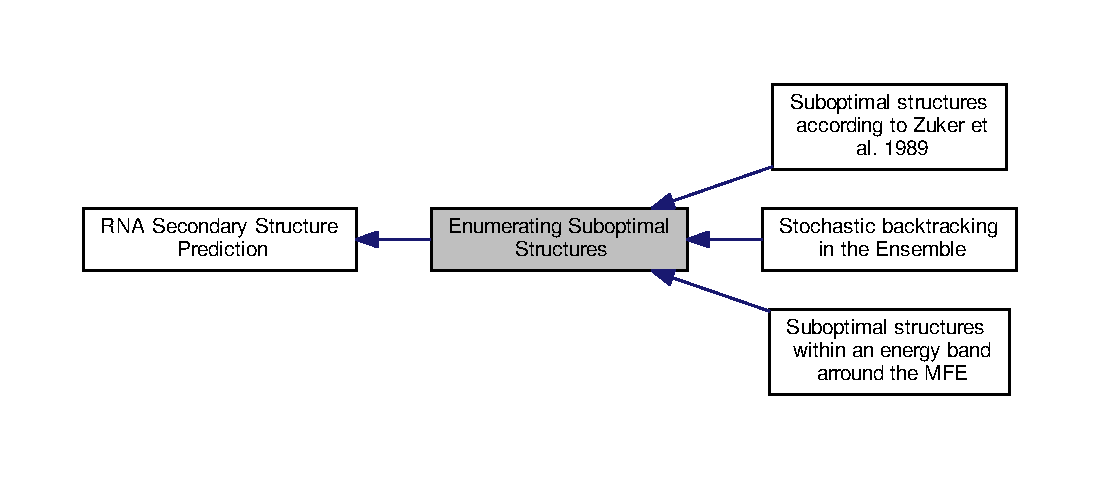
\includegraphics[width=350pt]{group__subopt__fold}
\end{center}
\end{figure}
\subsection*{Modules}
\begin{DoxyCompactItemize}
\item 
\hyperlink{group__subopt__zuker}{Suboptimal structures according to Zuker et al. 1989}
\item 
\hyperlink{group__subopt__wuchty}{Suboptimal structures within an energy band arround the M\+F\+E}
\item 
\hyperlink{group__subopt__stochbt}{Stochastic backtracking in the Ensemble}
\end{DoxyCompactItemize}
\subsection*{Files}
\begin{DoxyCompactItemize}
\item 
file \hyperlink{subopt_8h}{subopt.\+h}
\begin{DoxyCompactList}\small\item\em R\+N\+Asubopt and density of states declarations. \end{DoxyCompactList}\end{DoxyCompactItemize}


\subsection{Detailed Description}

\include{group__subopt__zuker}
\hypertarget{group__subopt__wuchty}{}\section{Suboptimal structures within an energy band arround the M\+F\+E}
\label{group__subopt__wuchty}\index{Suboptimal structures within an energy band arround the M\+F\+E@{Suboptimal structures within an energy band arround the M\+F\+E}}
Collaboration diagram for Suboptimal structures within an energy band arround the M\+F\+E\+:
\nopagebreak
\begin{figure}[H]
\begin{center}
\leavevmode
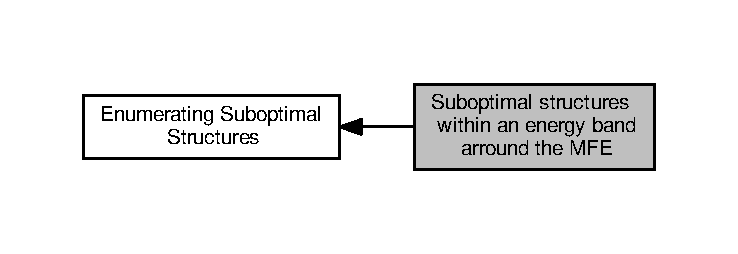
\includegraphics[width=350pt]{group__subopt__wuchty}
\end{center}
\end{figure}
\subsection*{Functions}
\begin{DoxyCompactItemize}
\item 
\hyperlink{structvrna__subopt__sol__s}{vrna\+\_\+subopt\+\_\+solution\+\_\+t} $\ast$ \hyperlink{group__subopt__wuchty_ga7988544ae3fc6334c1517cf76e5660aa}{vrna\+\_\+subopt} (\hyperlink{group__fold__compound_ga1b0cef17fd40466cef5968eaeeff6166}{vrna\+\_\+fold\+\_\+compound\+\_\+t} $\ast$vc, int delta, int sorted, F\+I\+L\+E $\ast$fp)
\begin{DoxyCompactList}\small\item\em Returns list of subopt structures or writes to fp. \end{DoxyCompactList}\item 
\hyperlink{structvrna__subopt__sol__s}{S\+O\+L\+U\+T\+I\+O\+N} $\ast$ \hyperlink{group__subopt__wuchty_ga700f662506a233e42dd7fda74fafd40e}{subopt} (char $\ast$seq, char $\ast$structure, int delta, F\+I\+L\+E $\ast$fp)
\begin{DoxyCompactList}\small\item\em Returns list of subopt structures or writes to fp. \end{DoxyCompactList}\item 
\hypertarget{group__subopt__wuchty_gaa1e1e7031a948ebcb39a9d58d1e9842c}{}\hyperlink{structvrna__subopt__sol__s}{S\+O\+L\+U\+T\+I\+O\+N} $\ast$ \hyperlink{group__subopt__wuchty_gaa1e1e7031a948ebcb39a9d58d1e9842c}{subopt\+\_\+par} (char $\ast$seq, char $\ast$structure, \hyperlink{group__energy__parameters_ga8a69ca7d787e4fd6079914f5343a1f35}{vrna\+\_\+param\+\_\+t} $\ast$parameters, int delta, int is\+\_\+constrained, int is\+\_\+circular, F\+I\+L\+E $\ast$fp)\label{group__subopt__wuchty_gaa1e1e7031a948ebcb39a9d58d1e9842c}

\begin{DoxyCompactList}\small\item\em Returns list of subopt structures or writes to fp. \end{DoxyCompactList}\item 
\hyperlink{structvrna__subopt__sol__s}{S\+O\+L\+U\+T\+I\+O\+N} $\ast$ \hyperlink{group__subopt__wuchty_ga8634516e4740e0b6c9a46d2bae940340}{subopt\+\_\+circ} (char $\ast$seq, char $\ast$sequence, int delta, F\+I\+L\+E $\ast$fp)
\begin{DoxyCompactList}\small\item\em Returns list of circular subopt structures or writes to fp. \end{DoxyCompactList}\end{DoxyCompactItemize}
\subsection*{Variables}
\begin{DoxyCompactItemize}
\item 
\hypertarget{group__subopt__wuchty_ga5e57d914bcb5feeecdf520e25313fcfe}{}double \hyperlink{group__subopt__wuchty_ga5e57d914bcb5feeecdf520e25313fcfe}{print\+\_\+energy}\label{group__subopt__wuchty_ga5e57d914bcb5feeecdf520e25313fcfe}

\begin{DoxyCompactList}\small\item\em printing threshold for use with log\+M\+L \end{DoxyCompactList}\item 
\hypertarget{group__subopt__wuchty_ga873cf8ed69e0437f8efa8b1fec854a0e}{}int \hyperlink{group__subopt__wuchty_ga873cf8ed69e0437f8efa8b1fec854a0e}{subopt\+\_\+sorted}\label{group__subopt__wuchty_ga873cf8ed69e0437f8efa8b1fec854a0e}

\begin{DoxyCompactList}\small\item\em Sort output by energy. \end{DoxyCompactList}\end{DoxyCompactItemize}


\subsection{Detailed Description}


\subsection{Function Documentation}
\hypertarget{group__subopt__wuchty_ga7988544ae3fc6334c1517cf76e5660aa}{}\index{Suboptimal structures within an energy band arround the M\+F\+E@{Suboptimal structures within an energy band arround the M\+F\+E}!vrna\+\_\+subopt@{vrna\+\_\+subopt}}
\index{vrna\+\_\+subopt@{vrna\+\_\+subopt}!Suboptimal structures within an energy band arround the M\+F\+E@{Suboptimal structures within an energy band arround the M\+F\+E}}
\subsubsection[{vrna\+\_\+subopt}]{\setlength{\rightskip}{0pt plus 5cm}{\bf vrna\+\_\+subopt\+\_\+solution\+\_\+t}$\ast$ vrna\+\_\+subopt (
\begin{DoxyParamCaption}
\item[{{\bf vrna\+\_\+fold\+\_\+compound\+\_\+t} $\ast$}]{vc, }
\item[{int}]{delta, }
\item[{int}]{sorted, }
\item[{F\+I\+L\+E $\ast$}]{fp}
\end{DoxyParamCaption}
)}\label{group__subopt__wuchty_ga7988544ae3fc6334c1517cf76e5660aa}


{\ttfamily \#include $<$\hyperlink{subopt_8h}{Vienna\+R\+N\+A/subopt.\+h}$>$}



Returns list of subopt structures or writes to fp. 

This function produces {\bfseries all} suboptimal secondary structures within \textquotesingle{}delta\textquotesingle{} $\ast$ 0.\+01 kcal/mol of the optimum, see \cite{wuchty:1999}. The results are either directly written to a \textquotesingle{}fp\textquotesingle{} (if \textquotesingle{}fp\textquotesingle{} is not N\+U\+L\+L), or (fp==N\+U\+L\+L) returned in a \#vrna\+\_\+subopt\+\_\+solution\+\_\+t $\ast$ list terminated by an entry were the \textquotesingle{}structure\textquotesingle{} member is N\+U\+L\+L.

\begin{DoxySeeAlso}{See also}
\hyperlink{group__subopt__zuker_gac0df98085abd242c7a6b1c868b3a35c8}{vrna\+\_\+subopt\+\_\+zuker()} 
\end{DoxySeeAlso}

\begin{DoxyParams}{Parameters}
{\em vc} & \\
\hline
{\em delta} & \\
\hline
{\em sorted} & Sort results by energy in ascending order \\
\hline
{\em fp} & \\
\hline
\end{DoxyParams}
\begin{DoxyReturn}{Returns}

\end{DoxyReturn}
\hypertarget{group__subopt__wuchty_ga700f662506a233e42dd7fda74fafd40e}{}\index{Suboptimal structures within an energy band arround the M\+F\+E@{Suboptimal structures within an energy band arround the M\+F\+E}!subopt@{subopt}}
\index{subopt@{subopt}!Suboptimal structures within an energy band arround the M\+F\+E@{Suboptimal structures within an energy band arround the M\+F\+E}}
\subsubsection[{subopt}]{\setlength{\rightskip}{0pt plus 5cm}{\bf S\+O\+L\+U\+T\+I\+O\+N}$\ast$ subopt (
\begin{DoxyParamCaption}
\item[{char $\ast$}]{seq, }
\item[{char $\ast$}]{structure, }
\item[{int}]{delta, }
\item[{F\+I\+L\+E $\ast$}]{fp}
\end{DoxyParamCaption}
)}\label{group__subopt__wuchty_ga700f662506a233e42dd7fda74fafd40e}


{\ttfamily \#include $<$\hyperlink{subopt_8h}{Vienna\+R\+N\+A/subopt.\+h}$>$}



Returns list of subopt structures or writes to fp. 

This function produces {\bfseries all} suboptimal secondary structures within \textquotesingle{}delta\textquotesingle{} $\ast$ 0.\+01 kcal/mol of the optimum. The results are either directly written to a \textquotesingle{}fp\textquotesingle{} (if \textquotesingle{}fp\textquotesingle{} is not N\+U\+L\+L), or (fp==N\+U\+L\+L) returned in a \#\+S\+O\+L\+U\+T\+I\+O\+N $\ast$ list terminated by an entry were the \textquotesingle{}structure\textquotesingle{} pointer is N\+U\+L\+L.


\begin{DoxyParams}{Parameters}
{\em seq} & \\
\hline
{\em structure} & \\
\hline
{\em delta} & \\
\hline
{\em fp} & \\
\hline
\end{DoxyParams}
\begin{DoxyReturn}{Returns}

\end{DoxyReturn}
\hypertarget{group__subopt__wuchty_ga8634516e4740e0b6c9a46d2bae940340}{}\index{Suboptimal structures within an energy band arround the M\+F\+E@{Suboptimal structures within an energy band arround the M\+F\+E}!subopt\+\_\+circ@{subopt\+\_\+circ}}
\index{subopt\+\_\+circ@{subopt\+\_\+circ}!Suboptimal structures within an energy band arround the M\+F\+E@{Suboptimal structures within an energy band arround the M\+F\+E}}
\subsubsection[{subopt\+\_\+circ}]{\setlength{\rightskip}{0pt plus 5cm}{\bf S\+O\+L\+U\+T\+I\+O\+N}$\ast$ subopt\+\_\+circ (
\begin{DoxyParamCaption}
\item[{char $\ast$}]{seq, }
\item[{char $\ast$}]{sequence, }
\item[{int}]{delta, }
\item[{F\+I\+L\+E $\ast$}]{fp}
\end{DoxyParamCaption}
)}\label{group__subopt__wuchty_ga8634516e4740e0b6c9a46d2bae940340}


{\ttfamily \#include $<$\hyperlink{subopt_8h}{Vienna\+R\+N\+A/subopt.\+h}$>$}



Returns list of circular subopt structures or writes to fp. 

This function is similar to \hyperlink{group__subopt__wuchty_ga700f662506a233e42dd7fda74fafd40e}{subopt()} but calculates secondary structures assuming the R\+N\+A sequence to be circular instead of linear


\begin{DoxyParams}{Parameters}
{\em seq} & \\
\hline
{\em sequence} & \\
\hline
{\em delta} & \\
\hline
{\em fp} & \\
\hline
\end{DoxyParams}
\begin{DoxyReturn}{Returns}

\end{DoxyReturn}

\hypertarget{group__subopt__stochbt}{\section{Stochastic backtracking in the Ensemble}
\label{group__subopt__stochbt}\index{Stochastic backtracking in the Ensemble@{Stochastic backtracking in the Ensemble}}
}
Collaboration diagram for Stochastic backtracking in the Ensemble\+:
\nopagebreak
\begin{figure}[H]
\begin{center}
\leavevmode
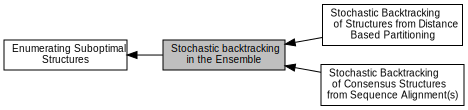
\includegraphics[width=350pt]{group__subopt__stochbt}
\end{center}
\end{figure}
\subsection*{Modules}
\begin{DoxyCompactItemize}
\item 
\hyperlink{group__consensus__stochbt}{Stochastic Backtracking of Consensus Structures from Sequence Alignment(s)}
\item 
\hyperlink{group__kl__neighborhood__stochbt}{Stochastic Backtracking of Structures from Distance Based Partitioning}
\begin{DoxyCompactList}\small\item\em Contains functions related to stochastic backtracking from a specified distance class. \end{DoxyCompactList}\end{DoxyCompactItemize}
\subsection*{Functions}
\begin{DoxyCompactItemize}
\item 
char $\ast$ \hyperlink{group__subopt__stochbt_ga5a3e11d3ce121b5b045cb57f86a8ed05}{vrna\+\_\+pbacktrack5} (\hyperlink{group__fold__compound_ga1b0cef17fd40466cef5968eaeeff6166}{vrna\+\_\+fold\+\_\+compound\+\_\+t} $\ast$vc, int length)
\begin{DoxyCompactList}\small\item\em Sample a secondary structure of a subsequence from the Boltzmann ensemble according its probability. \end{DoxyCompactList}\item 
char $\ast$ \hyperlink{group__subopt__stochbt_ga0429de82e75af6c6e7508f4d273a192f}{vrna\+\_\+pbacktrack} (\hyperlink{group__fold__compound_ga1b0cef17fd40466cef5968eaeeff6166}{vrna\+\_\+fold\+\_\+compound\+\_\+t} $\ast$vc)
\begin{DoxyCompactList}\small\item\em Sample a secondary structure (consensus structure) from the Boltzmann ensemble according its probability. \end{DoxyCompactList}\item 
char $\ast$ \hyperlink{group__subopt__stochbt_gac03ca6db186bb3bf0a2a326d7fb3ba03}{pbacktrack} (char $\ast$sequence)
\begin{DoxyCompactList}\small\item\em Sample a secondary structure from the Boltzmann ensemble according its probability. \end{DoxyCompactList}\item 
char $\ast$ \hyperlink{group__subopt__stochbt_ga00474051204ac9ad576b3e45174d03ff}{pbacktrack\+\_\+circ} (char $\ast$sequence)
\begin{DoxyCompactList}\small\item\em Sample a secondary structure of a circular R\+N\+A from the Boltzmann ensemble according its probability. \end{DoxyCompactList}\end{DoxyCompactItemize}
\subsection*{Variables}
\begin{DoxyCompactItemize}
\item 
int \hyperlink{group__subopt__stochbt_gacd79b1a570e6ad9be24cb11fe8cae30a}{st\+\_\+back}
\begin{DoxyCompactList}\small\item\em Flag indicating that auxilary arrays are needed throughout the computations. This is essential for stochastic backtracking. \end{DoxyCompactList}\end{DoxyCompactItemize}


\subsection{Detailed Description}


\subsection{Function Documentation}
\hypertarget{group__subopt__stochbt_ga5a3e11d3ce121b5b045cb57f86a8ed05}{\index{Stochastic backtracking in the Ensemble@{Stochastic backtracking in the Ensemble}!vrna\+\_\+pbacktrack5@{vrna\+\_\+pbacktrack5}}
\index{vrna\+\_\+pbacktrack5@{vrna\+\_\+pbacktrack5}!Stochastic backtracking in the Ensemble@{Stochastic backtracking in the Ensemble}}
\subsubsection[{vrna\+\_\+pbacktrack5}]{\setlength{\rightskip}{0pt plus 5cm}char$\ast$ vrna\+\_\+pbacktrack5 (
\begin{DoxyParamCaption}
\item[{{\bf vrna\+\_\+fold\+\_\+compound\+\_\+t} $\ast$}]{vc, }
\item[{int}]{length}
\end{DoxyParamCaption}
)}}\label{group__subopt__stochbt_ga5a3e11d3ce121b5b045cb57f86a8ed05}


{\ttfamily \#include $<$\hyperlink{boltzmann__sampling_8h}{Vienna\+R\+N\+A/boltzmann\+\_\+sampling.\+h}$>$}



Sample a secondary structure of a subsequence from the Boltzmann ensemble according its probability. 

\begin{DoxyPrecond}{Precondition}
The fold compound has to be obtained using the \#\+V\+R\+N\+A\+\_\+\+O\+P\+T\+I\+O\+N\+\_\+\+H\+Y\+B\+R\+I\+D option in \hyperlink{group__fold__compound_ga6601d994ba32b11511b36f68b08403be}{vrna\+\_\+fold\+\_\+compound()} 

\hyperlink{group__pf__fold_ga29e256d688ad221b78d37f427e0e99bc}{vrna\+\_\+pf()} has to be called first to fill the partition function matrices
\end{DoxyPrecond}

\begin{DoxyParams}{Parameters}
{\em vc} & The fold compound data structure \\
\hline
{\em length} & The length of the subsequence to consider (starting with 5' end) \\
\hline
\end{DoxyParams}
\begin{DoxyReturn}{Returns}
A sampled secondary structure in dot-\/bracket notation 
\end{DoxyReturn}
\hypertarget{group__subopt__stochbt_ga0429de82e75af6c6e7508f4d273a192f}{\index{Stochastic backtracking in the Ensemble@{Stochastic backtracking in the Ensemble}!vrna\+\_\+pbacktrack@{vrna\+\_\+pbacktrack}}
\index{vrna\+\_\+pbacktrack@{vrna\+\_\+pbacktrack}!Stochastic backtracking in the Ensemble@{Stochastic backtracking in the Ensemble}}
\subsubsection[{vrna\+\_\+pbacktrack}]{\setlength{\rightskip}{0pt plus 5cm}char$\ast$ vrna\+\_\+pbacktrack (
\begin{DoxyParamCaption}
\item[{{\bf vrna\+\_\+fold\+\_\+compound\+\_\+t} $\ast$}]{vc}
\end{DoxyParamCaption}
)}}\label{group__subopt__stochbt_ga0429de82e75af6c6e7508f4d273a192f}


{\ttfamily \#include $<$\hyperlink{boltzmann__sampling_8h}{Vienna\+R\+N\+A/boltzmann\+\_\+sampling.\+h}$>$}



Sample a secondary structure (consensus structure) from the Boltzmann ensemble according its probability. 

\begin{DoxyPrecond}{Precondition}
The dynamic programming (D\+P) matrices have to allow for unique multibranch loop decomposition, i.\+e. the \hyperlink{group__model__details_ade065b814a4e2e72ead93ab502613ed2}{vrna\+\_\+md\+\_\+t.\+uniq\+\_\+\+M\+L} flag has to be non-\/zero before calling \hyperlink{group__fold__compound_ga6601d994ba32b11511b36f68b08403be}{vrna\+\_\+fold\+\_\+compound()} 

\hyperlink{group__pf__fold_ga29e256d688ad221b78d37f427e0e99bc}{vrna\+\_\+pf()} has to be called first to fill the partition function matrices
\end{DoxyPrecond}
\begin{DoxyNote}{Note}
This function is polymorphic. It accepts \hyperlink{group__fold__compound_ga1b0cef17fd40466cef5968eaeeff6166}{vrna\+\_\+fold\+\_\+compound\+\_\+t} of type \hyperlink{group__fold__compound_gga01a4ff86fa71deaaa5d1abbd95a1447da1608d3aa78905fc39e0d25a624ac9512}{V\+R\+N\+A\+\_\+\+V\+C\+\_\+\+T\+Y\+P\+E\+\_\+\+S\+I\+N\+G\+L\+E}, and \hyperlink{group__fold__compound_gga01a4ff86fa71deaaa5d1abbd95a1447da056345f1bcfe7cd595d1fd437c05246d}{V\+R\+N\+A\+\_\+\+V\+C\+\_\+\+T\+Y\+P\+E\+\_\+\+A\+L\+I\+G\+N\+M\+E\+N\+T}.

The function will automagically detect cicular R\+N\+As based on the model\+\_\+details in exp\+\_\+params as provided via the \hyperlink{group__fold__compound_ga1b0cef17fd40466cef5968eaeeff6166}{vrna\+\_\+fold\+\_\+compound\+\_\+t}
\end{DoxyNote}

\begin{DoxyParams}{Parameters}
{\em vc} & The fold compound data structure \\
\hline
{\em length} & The length of the subsequence to consider (starting with 5' end) \\
\hline
\end{DoxyParams}
\begin{DoxyReturn}{Returns}
A sampled secondary structure in dot-\/bracket notation 
\end{DoxyReturn}
\hypertarget{group__subopt__stochbt_gac03ca6db186bb3bf0a2a326d7fb3ba03}{\index{Stochastic backtracking in the Ensemble@{Stochastic backtracking in the Ensemble}!pbacktrack@{pbacktrack}}
\index{pbacktrack@{pbacktrack}!Stochastic backtracking in the Ensemble@{Stochastic backtracking in the Ensemble}}
\subsubsection[{pbacktrack}]{\setlength{\rightskip}{0pt plus 5cm}char$\ast$ pbacktrack (
\begin{DoxyParamCaption}
\item[{char $\ast$}]{sequence}
\end{DoxyParamCaption}
)}}\label{group__subopt__stochbt_gac03ca6db186bb3bf0a2a326d7fb3ba03}


{\ttfamily \#include $<$\hyperlink{part__func_8h}{Vienna\+R\+N\+A/part\+\_\+func.\+h}$>$}



Sample a secondary structure from the Boltzmann ensemble according its probability. 

\begin{DoxyPrecond}{Precondition}
\hyperlink{group__subopt__stochbt_gacd79b1a570e6ad9be24cb11fe8cae30a}{st\+\_\+back} has to be set to 1 before calling \hyperlink{group__pf__fold_gadc3db3d98742427e7001a7fd36ef28c2}{pf\+\_\+fold()} or \hyperlink{group__pf__fold_gac4f95bee734b2563a3d6e9932117ebdf}{pf\+\_\+fold\+\_\+par()} 

\hyperlink{group__pf__fold_gac4f95bee734b2563a3d6e9932117ebdf}{pf\+\_\+fold\+\_\+par()} or \hyperlink{group__pf__fold_gadc3db3d98742427e7001a7fd36ef28c2}{pf\+\_\+fold()} have to be called first to fill the partition function matrices
\end{DoxyPrecond}

\begin{DoxyParams}{Parameters}
{\em sequence} & The R\+N\+A sequence \\
\hline
\end{DoxyParams}
\begin{DoxyReturn}{Returns}
A sampled secondary structure in dot-\/bracket notation 
\end{DoxyReturn}
\hypertarget{group__subopt__stochbt_ga00474051204ac9ad576b3e45174d03ff}{\index{Stochastic backtracking in the Ensemble@{Stochastic backtracking in the Ensemble}!pbacktrack\+\_\+circ@{pbacktrack\+\_\+circ}}
\index{pbacktrack\+\_\+circ@{pbacktrack\+\_\+circ}!Stochastic backtracking in the Ensemble@{Stochastic backtracking in the Ensemble}}
\subsubsection[{pbacktrack\+\_\+circ}]{\setlength{\rightskip}{0pt plus 5cm}char$\ast$ pbacktrack\+\_\+circ (
\begin{DoxyParamCaption}
\item[{char $\ast$}]{sequence}
\end{DoxyParamCaption}
)}}\label{group__subopt__stochbt_ga00474051204ac9ad576b3e45174d03ff}


{\ttfamily \#include $<$\hyperlink{part__func_8h}{Vienna\+R\+N\+A/part\+\_\+func.\+h}$>$}



Sample a secondary structure of a circular R\+N\+A from the Boltzmann ensemble according its probability. 

This function does the same as \hyperlink{group__subopt__stochbt_gac03ca6db186bb3bf0a2a326d7fb3ba03}{pbacktrack()} but assumes the R\+N\+A molecule to be circular

\begin{DoxyPrecond}{Precondition}
\hyperlink{group__subopt__stochbt_gacd79b1a570e6ad9be24cb11fe8cae30a}{st\+\_\+back} has to be set to 1 before calling \hyperlink{group__pf__fold_gadc3db3d98742427e7001a7fd36ef28c2}{pf\+\_\+fold()} or \hyperlink{group__pf__fold_gac4f95bee734b2563a3d6e9932117ebdf}{pf\+\_\+fold\+\_\+par()} 

\hyperlink{group__pf__fold_gac4f95bee734b2563a3d6e9932117ebdf}{pf\+\_\+fold\+\_\+par()} or \hyperlink{group__pf__fold_ga819ce5fca8984004ac81c4a3b04cb735}{pf\+\_\+circ\+\_\+fold()} have to be called first to fill the partition function matrices
\end{DoxyPrecond}
\begin{DoxyRefDesc}{Deprecated}
\item[\hyperlink{deprecated__deprecated000096}{Deprecated}]Use \hyperlink{group__subopt__stochbt_ga0429de82e75af6c6e7508f4d273a192f}{vrna\+\_\+pbacktrack()} instead.\end{DoxyRefDesc}



\begin{DoxyParams}{Parameters}
{\em sequence} & The R\+N\+A sequence \\
\hline
\end{DoxyParams}
\begin{DoxyReturn}{Returns}
A sampled secondary structure in dot-\/bracket notation 
\end{DoxyReturn}


\subsection{Variable Documentation}
\hypertarget{group__subopt__stochbt_gacd79b1a570e6ad9be24cb11fe8cae30a}{\index{Stochastic backtracking in the Ensemble@{Stochastic backtracking in the Ensemble}!st\+\_\+back@{st\+\_\+back}}
\index{st\+\_\+back@{st\+\_\+back}!Stochastic backtracking in the Ensemble@{Stochastic backtracking in the Ensemble}}
\subsubsection[{st\+\_\+back}]{\setlength{\rightskip}{0pt plus 5cm}int st\+\_\+back}}\label{group__subopt__stochbt_gacd79b1a570e6ad9be24cb11fe8cae30a}


{\ttfamily \#include $<$\hyperlink{part__func_8h}{Vienna\+R\+N\+A/part\+\_\+func.\+h}$>$}



Flag indicating that auxilary arrays are needed throughout the computations. This is essential for stochastic backtracking. 

Set this variable to 1 prior to a call of \hyperlink{group__pf__fold_gadc3db3d98742427e7001a7fd36ef28c2}{pf\+\_\+fold()} to ensure that all matrices needed for stochastic backtracking are filled in the forward recursions

\begin{DoxyRefDesc}{Deprecated}
\item[\hyperlink{deprecated__deprecated000093}{Deprecated}]set the {\itshape uniq\+\_\+\+M\+L} flag in \hyperlink{group__model__details_ga1f8a10e12a0a1915f2a4eff0b28ea17c}{vrna\+\_\+md\+\_\+t} before passing it to \hyperlink{group__fold__compound_ga6601d994ba32b11511b36f68b08403be}{vrna\+\_\+fold\+\_\+compound()}.\end{DoxyRefDesc}


\begin{DoxySeeAlso}{See also}
\hyperlink{group__subopt__stochbt_gac03ca6db186bb3bf0a2a326d7fb3ba03}{pbacktrack()}, \hyperlink{group__subopt__stochbt_ga00474051204ac9ad576b3e45174d03ff}{pbacktrack\+\_\+circ} 
\end{DoxySeeAlso}

\include{group__cofold}
\include{group__mfe__fold__single}
\hypertarget{group__mfe__cofold}{}\section{M\+F\+E Structures of two hybridized Sequences}
\label{group__mfe__cofold}\index{M\+F\+E Structures of two hybridized Sequences@{M\+F\+E Structures of two hybridized Sequences}}
Collaboration diagram for M\+F\+E Structures of two hybridized Sequences\+:
\nopagebreak
\begin{figure}[H]
\begin{center}
\leavevmode
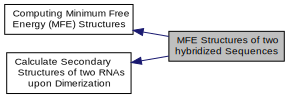
\includegraphics[width=350pt]{group__mfe__cofold}
\end{center}
\end{figure}
\subsection*{Files}
\begin{DoxyCompactItemize}
\item 
file \hyperlink{cofold_8h}{cofold.\+h}
\begin{DoxyCompactList}\small\item\em M\+F\+E version of cofolding routines. \end{DoxyCompactList}\end{DoxyCompactItemize}
\subsection*{Functions}
\begin{DoxyCompactItemize}
\item 
float \hyperlink{group__mfe__cofold_ga45515db181f17653ef7ef5487ef36d08}{vrna\+\_\+cofold} (const char $\ast$string, char $\ast$structure)
\begin{DoxyCompactList}\small\item\em Compute Minimum Free Energy (M\+F\+E), and a corresponding secondary structure for two dimerized R\+N\+A sequences. \end{DoxyCompactList}\item 
float \hyperlink{group__mfe__cofold_gabc8517f22cfe70595ee81fc837910d52}{cofold} (const char $\ast$sequence, char $\ast$structure)
\begin{DoxyCompactList}\small\item\em Compute the minimum free energy of two interacting R\+N\+A molecules. \end{DoxyCompactList}\item 
float \hyperlink{group__mfe__cofold_ga7612cfeeb1b793f1e4179b1eb53df1f3}{cofold\+\_\+par} (const char $\ast$string, char $\ast$structure, \hyperlink{group__energy__parameters_ga8a69ca7d787e4fd6079914f5343a1f35}{vrna\+\_\+param\+\_\+t} $\ast$parameters, int is\+\_\+constrained)
\begin{DoxyCompactList}\small\item\em Compute the minimum free energy of two interacting R\+N\+A molecules. \end{DoxyCompactList}\item 
void \hyperlink{group__mfe__cofold_gaafb33d7473eb9af9d1b168ca8761c41a}{free\+\_\+co\+\_\+arrays} (void)
\begin{DoxyCompactList}\small\item\em Free memory occupied by \hyperlink{group__mfe__cofold_gabc8517f22cfe70595ee81fc837910d52}{cofold()} \end{DoxyCompactList}\item 
void \hyperlink{group__mfe__cofold_ga4fcbf34e77b99bfbb2333d2ab0c41a57}{update\+\_\+cofold\+\_\+params} (void)
\begin{DoxyCompactList}\small\item\em Recalculate parameters. \end{DoxyCompactList}\item 
void \hyperlink{group__mfe__cofold_gaaadbd28b4e428710529ab4098fdacad3}{update\+\_\+cofold\+\_\+params\+\_\+par} (\hyperlink{group__energy__parameters_ga8a69ca7d787e4fd6079914f5343a1f35}{vrna\+\_\+param\+\_\+t} $\ast$parameters)
\begin{DoxyCompactList}\small\item\em Recalculate parameters. \end{DoxyCompactList}\item 
void \hyperlink{group__mfe__cofold_ga5f5bf4df35d0554f6ace9579f8744c48}{export\+\_\+cofold\+\_\+arrays\+\_\+gq} (int $\ast$$\ast$f5\+\_\+p, int $\ast$$\ast$c\+\_\+p, int $\ast$$\ast$f\+M\+L\+\_\+p, int $\ast$$\ast$f\+M1\+\_\+p, int $\ast$$\ast$fc\+\_\+p, int $\ast$$\ast$ggg\+\_\+p, int $\ast$$\ast$indx\+\_\+p, char $\ast$$\ast$ptype\+\_\+p)
\begin{DoxyCompactList}\small\item\em Export the arrays of partition function cofold (with gquadruplex support) \end{DoxyCompactList}\item 
void \hyperlink{group__mfe__cofold_ga5cb6b59983f1f74ccc00b9b9c4e84482}{export\+\_\+cofold\+\_\+arrays} (int $\ast$$\ast$f5\+\_\+p, int $\ast$$\ast$c\+\_\+p, int $\ast$$\ast$f\+M\+L\+\_\+p, int $\ast$$\ast$f\+M1\+\_\+p, int $\ast$$\ast$fc\+\_\+p, int $\ast$$\ast$indx\+\_\+p, char $\ast$$\ast$ptype\+\_\+p)
\begin{DoxyCompactList}\small\item\em Export the arrays of partition function cofold. \end{DoxyCompactList}\item 
void \hyperlink{group__mfe__cofold_ga4958b517c613e4d2afd5bce6c1060a79}{get\+\_\+monomere\+\_\+mfes} (float $\ast$e1, float $\ast$e2)
\begin{DoxyCompactList}\small\item\em get\+\_\+monomer\+\_\+free\+\_\+energies \end{DoxyCompactList}\item 
void \hyperlink{group__mfe__cofold_gafee0c32208aa2ac97338b6e3fbad7fa5}{initialize\+\_\+cofold} (int length)
\item 
float \hyperlink{group__mfe__cofold_gaab22d10c1190f205f16a77cab9d5d3ee}{vrna\+\_\+mfe\+\_\+dimer} (\hyperlink{group__fold__compound_ga1b0cef17fd40466cef5968eaeeff6166}{vrna\+\_\+fold\+\_\+compound\+\_\+t} $\ast$vc, char $\ast$structure)
\begin{DoxyCompactList}\small\item\em Compute the minimum free energy of two interacting R\+N\+A molecules. \end{DoxyCompactList}\end{DoxyCompactItemize}


\subsection{Detailed Description}


\subsection{Function Documentation}
\hypertarget{group__mfe__cofold_ga45515db181f17653ef7ef5487ef36d08}{}\index{M\+F\+E Structures of two hybridized Sequences@{M\+F\+E Structures of two hybridized Sequences}!vrna\+\_\+cofold@{vrna\+\_\+cofold}}
\index{vrna\+\_\+cofold@{vrna\+\_\+cofold}!M\+F\+E Structures of two hybridized Sequences@{M\+F\+E Structures of two hybridized Sequences}}
\subsubsection[{vrna\+\_\+cofold}]{\setlength{\rightskip}{0pt plus 5cm}float vrna\+\_\+cofold (
\begin{DoxyParamCaption}
\item[{const char $\ast$}]{string, }
\item[{char $\ast$}]{structure}
\end{DoxyParamCaption}
)}\label{group__mfe__cofold_ga45515db181f17653ef7ef5487ef36d08}


{\ttfamily \#include $<$\hyperlink{cofold_8h}{Vienna\+R\+N\+A/cofold.\+h}$>$}



Compute Minimum Free Energy (M\+F\+E), and a corresponding secondary structure for two dimerized R\+N\+A sequences. 

This simplified interface to \hyperlink{group__mfe__fold_gabd3b147371ccf25c577f88bbbaf159fd}{vrna\+\_\+mfe()} computes the M\+F\+E and, if required, a secondary structure for two R\+N\+A sequences upon dimerization using default options. Memory required for dynamic programming (D\+P) matrices will be allocated and free\textquotesingle{}d on-\/the-\/fly. Hence, after return of this function, the recursively filled matrices are not available any more for any post-\/processing, e.\+g. suboptimal backtracking, etc.

\begin{DoxyNote}{Note}
In case you want to use the filled D\+P matrices for any subsequent post-\/processing step, or you require other conditions than specified by the default model details, use \hyperlink{group__mfe__fold_gabd3b147371ccf25c577f88bbbaf159fd}{vrna\+\_\+mfe()}, and the data structure \hyperlink{group__fold__compound_ga1b0cef17fd40466cef5968eaeeff6166}{vrna\+\_\+fold\+\_\+compound\+\_\+t} instead.
\end{DoxyNote}
\begin{DoxySeeAlso}{See also}
\hyperlink{group__mfe__cofold_gaab22d10c1190f205f16a77cab9d5d3ee}{vrna\+\_\+mfe\+\_\+dimer()}, \hyperlink{group__fold__compound_ga6601d994ba32b11511b36f68b08403be}{vrna\+\_\+fold\+\_\+compound()}, \hyperlink{group__fold__compound_ga1b0cef17fd40466cef5968eaeeff6166}{vrna\+\_\+fold\+\_\+compound\+\_\+t}, \hyperlink{group__string__utils_ga74f05ece32ea73b59f84a7452afd5fae}{vrna\+\_\+cut\+\_\+point\+\_\+insert()}
\end{DoxySeeAlso}

\begin{DoxyParams}{Parameters}
{\em sequence} & two R\+N\+A sequences separated by the \textquotesingle{}\&\textquotesingle{} character \\
\hline
{\em structure} & A pointer to the character array where the secondary structure in dot-\/bracket notation will be written to \\
\hline
\end{DoxyParams}
\begin{DoxyReturn}{Returns}
the minimum free energy (M\+F\+E) in kcal/mol 
\end{DoxyReturn}
\hypertarget{group__mfe__cofold_gabc8517f22cfe70595ee81fc837910d52}{}\index{M\+F\+E Structures of two hybridized Sequences@{M\+F\+E Structures of two hybridized Sequences}!cofold@{cofold}}
\index{cofold@{cofold}!M\+F\+E Structures of two hybridized Sequences@{M\+F\+E Structures of two hybridized Sequences}}
\subsubsection[{cofold}]{\setlength{\rightskip}{0pt plus 5cm}float cofold (
\begin{DoxyParamCaption}
\item[{const char $\ast$}]{sequence, }
\item[{char $\ast$}]{structure}
\end{DoxyParamCaption}
)}\label{group__mfe__cofold_gabc8517f22cfe70595ee81fc837910d52}


{\ttfamily \#include $<$\hyperlink{cofold_8h}{Vienna\+R\+N\+A/cofold.\+h}$>$}



Compute the minimum free energy of two interacting R\+N\+A molecules. 

The code is analog to the \hyperlink{group__mfe__fold__single_gaadafcb0f140795ae62e5ca027e335a9b}{fold()} function. If \hyperlink{fold__vars_8h_ab9b2c3a37a5516614c06d0ab54b97cda}{cut\+\_\+point} ==-\/1 results should be the same as with \hyperlink{group__mfe__fold__single_gaadafcb0f140795ae62e5ca027e335a9b}{fold()}.

\begin{DoxyRefDesc}{Deprecated}
\item[\hyperlink{deprecated__deprecated000030}{Deprecated}]use \hyperlink{group__mfe__cofold_gaab22d10c1190f205f16a77cab9d5d3ee}{vrna\+\_\+mfe\+\_\+dimer()} instead\end{DoxyRefDesc}



\begin{DoxyParams}{Parameters}
{\em sequence} & The two sequences concatenated \\
\hline
{\em structure} & Will hold the barcket dot structure of the dimer molecule \\
\hline
\end{DoxyParams}
\begin{DoxyReturn}{Returns}
minimum free energy of the structure 
\end{DoxyReturn}
\hypertarget{group__mfe__cofold_ga7612cfeeb1b793f1e4179b1eb53df1f3}{}\index{M\+F\+E Structures of two hybridized Sequences@{M\+F\+E Structures of two hybridized Sequences}!cofold\+\_\+par@{cofold\+\_\+par}}
\index{cofold\+\_\+par@{cofold\+\_\+par}!M\+F\+E Structures of two hybridized Sequences@{M\+F\+E Structures of two hybridized Sequences}}
\subsubsection[{cofold\+\_\+par}]{\setlength{\rightskip}{0pt plus 5cm}float cofold\+\_\+par (
\begin{DoxyParamCaption}
\item[{const char $\ast$}]{string, }
\item[{char $\ast$}]{structure, }
\item[{{\bf vrna\+\_\+param\+\_\+t} $\ast$}]{parameters, }
\item[{int}]{is\+\_\+constrained}
\end{DoxyParamCaption}
)}\label{group__mfe__cofold_ga7612cfeeb1b793f1e4179b1eb53df1f3}


{\ttfamily \#include $<$\hyperlink{cofold_8h}{Vienna\+R\+N\+A/cofold.\+h}$>$}



Compute the minimum free energy of two interacting R\+N\+A molecules. 

\begin{DoxyRefDesc}{Deprecated}
\item[\hyperlink{deprecated__deprecated000031}{Deprecated}]use \hyperlink{group__mfe__cofold_gaab22d10c1190f205f16a77cab9d5d3ee}{vrna\+\_\+mfe\+\_\+dimer()} instead\end{DoxyRefDesc}
\hypertarget{group__mfe__cofold_gaafb33d7473eb9af9d1b168ca8761c41a}{}\index{M\+F\+E Structures of two hybridized Sequences@{M\+F\+E Structures of two hybridized Sequences}!free\+\_\+co\+\_\+arrays@{free\+\_\+co\+\_\+arrays}}
\index{free\+\_\+co\+\_\+arrays@{free\+\_\+co\+\_\+arrays}!M\+F\+E Structures of two hybridized Sequences@{M\+F\+E Structures of two hybridized Sequences}}
\subsubsection[{free\+\_\+co\+\_\+arrays}]{\setlength{\rightskip}{0pt plus 5cm}void free\+\_\+co\+\_\+arrays (
\begin{DoxyParamCaption}
\item[{void}]{}
\end{DoxyParamCaption}
)}\label{group__mfe__cofold_gaafb33d7473eb9af9d1b168ca8761c41a}


{\ttfamily \#include $<$\hyperlink{cofold_8h}{Vienna\+R\+N\+A/cofold.\+h}$>$}



Free memory occupied by \hyperlink{group__mfe__cofold_gabc8517f22cfe70595ee81fc837910d52}{cofold()} 

\begin{DoxyRefDesc}{Deprecated}
\item[\hyperlink{deprecated__deprecated000032}{Deprecated}]This function will only free memory allocated by a prior call of \hyperlink{group__mfe__cofold_gabc8517f22cfe70595ee81fc837910d52}{cofold()} or \hyperlink{group__mfe__cofold_ga7612cfeeb1b793f1e4179b1eb53df1f3}{cofold\+\_\+par()}. See \hyperlink{group__mfe__cofold_gaab22d10c1190f205f16a77cab9d5d3ee}{vrna\+\_\+mfe\+\_\+dimer()} for how to use the new A\+P\+I\end{DoxyRefDesc}


\begin{DoxyNote}{Note}
folding matrices now reside in the fold compound, and should be free\textquotesingle{}d there 
\end{DoxyNote}
\begin{DoxySeeAlso}{See also}
vrna\+\_\+fc\+\_\+destroy(), \hyperlink{group__mfe__cofold_gaab22d10c1190f205f16a77cab9d5d3ee}{vrna\+\_\+mfe\+\_\+dimer()} 
\end{DoxySeeAlso}
\hypertarget{group__mfe__cofold_ga4fcbf34e77b99bfbb2333d2ab0c41a57}{}\index{M\+F\+E Structures of two hybridized Sequences@{M\+F\+E Structures of two hybridized Sequences}!update\+\_\+cofold\+\_\+params@{update\+\_\+cofold\+\_\+params}}
\index{update\+\_\+cofold\+\_\+params@{update\+\_\+cofold\+\_\+params}!M\+F\+E Structures of two hybridized Sequences@{M\+F\+E Structures of two hybridized Sequences}}
\subsubsection[{update\+\_\+cofold\+\_\+params}]{\setlength{\rightskip}{0pt plus 5cm}void update\+\_\+cofold\+\_\+params (
\begin{DoxyParamCaption}
\item[{void}]{}
\end{DoxyParamCaption}
)}\label{group__mfe__cofold_ga4fcbf34e77b99bfbb2333d2ab0c41a57}


{\ttfamily \#include $<$\hyperlink{cofold_8h}{Vienna\+R\+N\+A/cofold.\+h}$>$}



Recalculate parameters. 

\begin{DoxyRefDesc}{Deprecated}
\item[\hyperlink{deprecated__deprecated000033}{Deprecated}]See \hyperlink{group__energy__parameters_ga5d1909208f7ea3baa98b75afaa1f62ca}{vrna\+\_\+params\+\_\+subst()} for an alternative using the new A\+P\+I \end{DoxyRefDesc}
\hypertarget{group__mfe__cofold_gaaadbd28b4e428710529ab4098fdacad3}{}\index{M\+F\+E Structures of two hybridized Sequences@{M\+F\+E Structures of two hybridized Sequences}!update\+\_\+cofold\+\_\+params\+\_\+par@{update\+\_\+cofold\+\_\+params\+\_\+par}}
\index{update\+\_\+cofold\+\_\+params\+\_\+par@{update\+\_\+cofold\+\_\+params\+\_\+par}!M\+F\+E Structures of two hybridized Sequences@{M\+F\+E Structures of two hybridized Sequences}}
\subsubsection[{update\+\_\+cofold\+\_\+params\+\_\+par}]{\setlength{\rightskip}{0pt plus 5cm}void update\+\_\+cofold\+\_\+params\+\_\+par (
\begin{DoxyParamCaption}
\item[{{\bf vrna\+\_\+param\+\_\+t} $\ast$}]{parameters}
\end{DoxyParamCaption}
)}\label{group__mfe__cofold_gaaadbd28b4e428710529ab4098fdacad3}


{\ttfamily \#include $<$\hyperlink{cofold_8h}{Vienna\+R\+N\+A/cofold.\+h}$>$}



Recalculate parameters. 

\begin{DoxyRefDesc}{Deprecated}
\item[\hyperlink{deprecated__deprecated000034}{Deprecated}]See \hyperlink{group__energy__parameters_ga5d1909208f7ea3baa98b75afaa1f62ca}{vrna\+\_\+params\+\_\+subst()} for an alternative using the new A\+P\+I \end{DoxyRefDesc}
\hypertarget{group__mfe__cofold_ga5f5bf4df35d0554f6ace9579f8744c48}{}\index{M\+F\+E Structures of two hybridized Sequences@{M\+F\+E Structures of two hybridized Sequences}!export\+\_\+cofold\+\_\+arrays\+\_\+gq@{export\+\_\+cofold\+\_\+arrays\+\_\+gq}}
\index{export\+\_\+cofold\+\_\+arrays\+\_\+gq@{export\+\_\+cofold\+\_\+arrays\+\_\+gq}!M\+F\+E Structures of two hybridized Sequences@{M\+F\+E Structures of two hybridized Sequences}}
\subsubsection[{export\+\_\+cofold\+\_\+arrays\+\_\+gq}]{\setlength{\rightskip}{0pt plus 5cm}void export\+\_\+cofold\+\_\+arrays\+\_\+gq (
\begin{DoxyParamCaption}
\item[{int $\ast$$\ast$}]{f5\+\_\+p, }
\item[{int $\ast$$\ast$}]{c\+\_\+p, }
\item[{int $\ast$$\ast$}]{f\+M\+L\+\_\+p, }
\item[{int $\ast$$\ast$}]{f\+M1\+\_\+p, }
\item[{int $\ast$$\ast$}]{fc\+\_\+p, }
\item[{int $\ast$$\ast$}]{ggg\+\_\+p, }
\item[{int $\ast$$\ast$}]{indx\+\_\+p, }
\item[{char $\ast$$\ast$}]{ptype\+\_\+p}
\end{DoxyParamCaption}
)}\label{group__mfe__cofold_ga5f5bf4df35d0554f6ace9579f8744c48}


{\ttfamily \#include $<$\hyperlink{cofold_8h}{Vienna\+R\+N\+A/cofold.\+h}$>$}



Export the arrays of partition function cofold (with gquadruplex support) 

Export the cofold arrays for use e.\+g. in the concentration Computations or suboptimal secondary structure backtracking

\begin{DoxyRefDesc}{Deprecated}
\item[\hyperlink{deprecated__deprecated000035}{Deprecated}]folding matrices now reside within the fold compound. Thus, this function will only work in conjunction with a prior call to \hyperlink{group__mfe__cofold_gabc8517f22cfe70595ee81fc837910d52}{cofold()} or \hyperlink{group__mfe__cofold_ga7612cfeeb1b793f1e4179b1eb53df1f3}{cofold\+\_\+par()}\end{DoxyRefDesc}


\begin{DoxySeeAlso}{See also}
\hyperlink{group__mfe__cofold_gaab22d10c1190f205f16a77cab9d5d3ee}{vrna\+\_\+mfe\+\_\+dimer()} for the new A\+P\+I
\end{DoxySeeAlso}

\begin{DoxyParams}{Parameters}
{\em f5\+\_\+p} & A pointer to the \textquotesingle{}f5\textquotesingle{} array, i.\+e. array conatining best free energy in interval \mbox{[}1,j\mbox{]} \\
\hline
{\em c\+\_\+p} & A pointer to the \textquotesingle{}c\textquotesingle{} array, i.\+e. array containing best free energy in interval \mbox{[}i,j\mbox{]} given that i pairs with j \\
\hline
{\em f\+M\+L\+\_\+p} & A pointer to the \textquotesingle{}M\textquotesingle{} array, i.\+e. array containing best free energy in interval \mbox{[}i,j\mbox{]} for any multiloop segment with at least one stem \\
\hline
{\em f\+M1\+\_\+p} & A pointer to the \textquotesingle{}M1\textquotesingle{} array, i.\+e. array containing best free energy in interval \mbox{[}i,j\mbox{]} for multiloop segment with exactly one stem \\
\hline
{\em fc\+\_\+p} & A pointer to the \textquotesingle{}fc\textquotesingle{} array, i.\+e. array ... \\
\hline
{\em ggg\+\_\+p} & A pointer to the \textquotesingle{}ggg\textquotesingle{} array, i.\+e. array containing best free energy of a gquadruplex delimited by \mbox{[}i,j\mbox{]} \\
\hline
{\em indx\+\_\+p} & A pointer to the indexing array used for accessing the energy matrices \\
\hline
{\em ptype\+\_\+p} & A pointer to the ptype array containing the base pair types for each possibility (i,j) \\
\hline
\end{DoxyParams}
\hypertarget{group__mfe__cofold_ga5cb6b59983f1f74ccc00b9b9c4e84482}{}\index{M\+F\+E Structures of two hybridized Sequences@{M\+F\+E Structures of two hybridized Sequences}!export\+\_\+cofold\+\_\+arrays@{export\+\_\+cofold\+\_\+arrays}}
\index{export\+\_\+cofold\+\_\+arrays@{export\+\_\+cofold\+\_\+arrays}!M\+F\+E Structures of two hybridized Sequences@{M\+F\+E Structures of two hybridized Sequences}}
\subsubsection[{export\+\_\+cofold\+\_\+arrays}]{\setlength{\rightskip}{0pt plus 5cm}void export\+\_\+cofold\+\_\+arrays (
\begin{DoxyParamCaption}
\item[{int $\ast$$\ast$}]{f5\+\_\+p, }
\item[{int $\ast$$\ast$}]{c\+\_\+p, }
\item[{int $\ast$$\ast$}]{f\+M\+L\+\_\+p, }
\item[{int $\ast$$\ast$}]{f\+M1\+\_\+p, }
\item[{int $\ast$$\ast$}]{fc\+\_\+p, }
\item[{int $\ast$$\ast$}]{indx\+\_\+p, }
\item[{char $\ast$$\ast$}]{ptype\+\_\+p}
\end{DoxyParamCaption}
)}\label{group__mfe__cofold_ga5cb6b59983f1f74ccc00b9b9c4e84482}


{\ttfamily \#include $<$\hyperlink{cofold_8h}{Vienna\+R\+N\+A/cofold.\+h}$>$}



Export the arrays of partition function cofold. 

Export the cofold arrays for use e.\+g. in the concentration Computations or suboptimal secondary structure backtracking

\begin{DoxyRefDesc}{Deprecated}
\item[\hyperlink{deprecated__deprecated000036}{Deprecated}]folding matrices now reside within the \hyperlink{group__fold__compound_ga1b0cef17fd40466cef5968eaeeff6166}{vrna\+\_\+fold\+\_\+compound\+\_\+t}. Thus, this function will only work in conjunction with a prior call to the deprecated functions \hyperlink{group__mfe__cofold_gabc8517f22cfe70595ee81fc837910d52}{cofold()} or \hyperlink{group__mfe__cofold_ga7612cfeeb1b793f1e4179b1eb53df1f3}{cofold\+\_\+par()}\end{DoxyRefDesc}


\begin{DoxySeeAlso}{See also}
\hyperlink{group__mfe__cofold_gaab22d10c1190f205f16a77cab9d5d3ee}{vrna\+\_\+mfe\+\_\+dimer()} for the new A\+P\+I
\end{DoxySeeAlso}

\begin{DoxyParams}{Parameters}
{\em f5\+\_\+p} & A pointer to the \textquotesingle{}f5\textquotesingle{} array, i.\+e. array conatining best free energy in interval \mbox{[}1,j\mbox{]} \\
\hline
{\em c\+\_\+p} & A pointer to the \textquotesingle{}c\textquotesingle{} array, i.\+e. array containing best free energy in interval \mbox{[}i,j\mbox{]} given that i pairs with j \\
\hline
{\em f\+M\+L\+\_\+p} & A pointer to the \textquotesingle{}M\textquotesingle{} array, i.\+e. array containing best free energy in interval \mbox{[}i,j\mbox{]} for any multiloop segment with at least one stem \\
\hline
{\em f\+M1\+\_\+p} & A pointer to the \textquotesingle{}M1\textquotesingle{} array, i.\+e. array containing best free energy in interval \mbox{[}i,j\mbox{]} for multiloop segment with exactly one stem \\
\hline
{\em fc\+\_\+p} & A pointer to the \textquotesingle{}fc\textquotesingle{} array, i.\+e. array ... \\
\hline
{\em indx\+\_\+p} & A pointer to the indexing array used for accessing the energy matrices \\
\hline
{\em ptype\+\_\+p} & A pointer to the ptype array containing the base pair types for each possibility (i,j) \\
\hline
\end{DoxyParams}
\hypertarget{group__mfe__cofold_ga4958b517c613e4d2afd5bce6c1060a79}{}\index{M\+F\+E Structures of two hybridized Sequences@{M\+F\+E Structures of two hybridized Sequences}!get\+\_\+monomere\+\_\+mfes@{get\+\_\+monomere\+\_\+mfes}}
\index{get\+\_\+monomere\+\_\+mfes@{get\+\_\+monomere\+\_\+mfes}!M\+F\+E Structures of two hybridized Sequences@{M\+F\+E Structures of two hybridized Sequences}}
\subsubsection[{get\+\_\+monomere\+\_\+mfes}]{\setlength{\rightskip}{0pt plus 5cm}void get\+\_\+monomere\+\_\+mfes (
\begin{DoxyParamCaption}
\item[{float $\ast$}]{e1, }
\item[{float $\ast$}]{e2}
\end{DoxyParamCaption}
)}\label{group__mfe__cofold_ga4958b517c613e4d2afd5bce6c1060a79}


{\ttfamily \#include $<$\hyperlink{cofold_8h}{Vienna\+R\+N\+A/cofold.\+h}$>$}



get\+\_\+monomer\+\_\+free\+\_\+energies 

Export monomer free energies out of cofold arrays \begin{DoxyRefDesc}{Deprecated}
\item[\hyperlink{deprecated__deprecated000037}{Deprecated}]\{This function is obsolete and will be removed soon!\}\end{DoxyRefDesc}



\begin{DoxyParams}{Parameters}
{\em e1} & A pointer to a variable where the energy of molecule A will be written to \\
\hline
{\em e2} & A pointer to a variable where the energy of molecule B will be written to \\
\hline
\end{DoxyParams}
\hypertarget{group__mfe__cofold_gafee0c32208aa2ac97338b6e3fbad7fa5}{}\index{M\+F\+E Structures of two hybridized Sequences@{M\+F\+E Structures of two hybridized Sequences}!initialize\+\_\+cofold@{initialize\+\_\+cofold}}
\index{initialize\+\_\+cofold@{initialize\+\_\+cofold}!M\+F\+E Structures of two hybridized Sequences@{M\+F\+E Structures of two hybridized Sequences}}
\subsubsection[{initialize\+\_\+cofold}]{\setlength{\rightskip}{0pt plus 5cm}void initialize\+\_\+cofold (
\begin{DoxyParamCaption}
\item[{int}]{length}
\end{DoxyParamCaption}
)}\label{group__mfe__cofold_gafee0c32208aa2ac97338b6e3fbad7fa5}


{\ttfamily \#include $<$\hyperlink{cofold_8h}{Vienna\+R\+N\+A/cofold.\+h}$>$}

allocate arrays for folding \begin{DoxyRefDesc}{Deprecated}
\item[\hyperlink{deprecated__deprecated000038}{Deprecated}]\{This function is obsolete and will be removed soon!\} \end{DoxyRefDesc}
\hypertarget{group__mfe__cofold_gaab22d10c1190f205f16a77cab9d5d3ee}{}\index{M\+F\+E Structures of two hybridized Sequences@{M\+F\+E Structures of two hybridized Sequences}!vrna\+\_\+mfe\+\_\+dimer@{vrna\+\_\+mfe\+\_\+dimer}}
\index{vrna\+\_\+mfe\+\_\+dimer@{vrna\+\_\+mfe\+\_\+dimer}!M\+F\+E Structures of two hybridized Sequences@{M\+F\+E Structures of two hybridized Sequences}}
\subsubsection[{vrna\+\_\+mfe\+\_\+dimer}]{\setlength{\rightskip}{0pt plus 5cm}float vrna\+\_\+mfe\+\_\+dimer (
\begin{DoxyParamCaption}
\item[{{\bf vrna\+\_\+fold\+\_\+compound\+\_\+t} $\ast$}]{vc, }
\item[{char $\ast$}]{structure}
\end{DoxyParamCaption}
)}\label{group__mfe__cofold_gaab22d10c1190f205f16a77cab9d5d3ee}


{\ttfamily \#include $<$\hyperlink{mfe_8h}{Vienna\+R\+N\+A/mfe.\+h}$>$}



Compute the minimum free energy of two interacting R\+N\+A molecules. 

The code is analog to the \hyperlink{group__mfe__fold_gabd3b147371ccf25c577f88bbbaf159fd}{vrna\+\_\+mfe()} function.


\begin{DoxyParams}{Parameters}
{\em vc} & fold compound \\
\hline
{\em structure} & Will hold the barcket dot structure of the dimer molecule \\
\hline
\end{DoxyParams}
\begin{DoxyReturn}{Returns}
minimum free energy of the structure 
\end{DoxyReturn}

\hypertarget{group__pf__cofold}{\section{Partition Function for two hybridized Sequences}
\label{group__pf__cofold}\index{Partition Function for two hybridized Sequences@{Partition Function for two hybridized Sequences}}
}


Partition Function Cofolding.  


Collaboration diagram for Partition Function for two hybridized Sequences\+:
\nopagebreak
\begin{figure}[H]
\begin{center}
\leavevmode
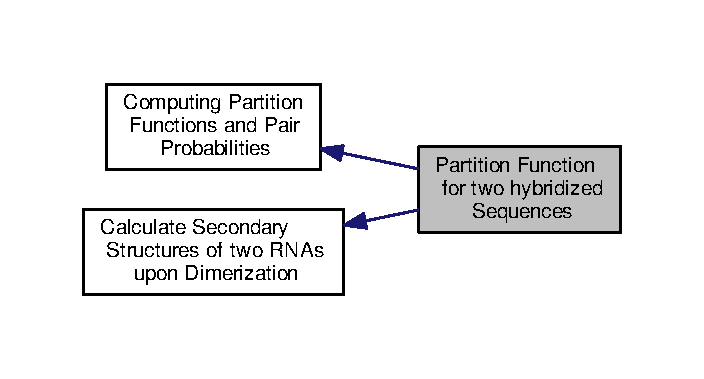
\includegraphics[width=338pt]{group__pf__cofold}
\end{center}
\end{figure}
\subsection*{Files}
\begin{DoxyCompactItemize}
\item 
file \hyperlink{part__func__co_8h}{part\+\_\+func\+\_\+co.\+h}
\begin{DoxyCompactList}\small\item\em Partition function for two R\+N\+A sequences. \end{DoxyCompactList}\end{DoxyCompactItemize}
\subsection*{Data Structures}
\begin{DoxyCompactItemize}
\item 
struct \hyperlink{group__pf__cofold_structvrna__dimer__pf__s}{vrna\+\_\+dimer\+\_\+pf\+\_\+s}
\item 
struct \hyperlink{group__pf__cofold_structvrna__dimer__conc__s}{vrna\+\_\+dimer\+\_\+conc\+\_\+s}
\end{DoxyCompactItemize}
\subsection*{Typedefs}
\begin{DoxyCompactItemize}
\item 
\hypertarget{group__pf__cofold_ga444df1587c9a2ca15b8eb25188f629c3}{typedef struct \hyperlink{group__pf__cofold_structvrna__dimer__pf__s}{vrna\+\_\+dimer\+\_\+pf\+\_\+s} \hyperlink{group__pf__cofold_ga444df1587c9a2ca15b8eb25188f629c3}{vrna\+\_\+dimer\+\_\+pf\+\_\+t}}\label{group__pf__cofold_ga444df1587c9a2ca15b8eb25188f629c3}

\begin{DoxyCompactList}\small\item\em Typename for the data structure that stores the dimer partition functions, \hyperlink{group__pf__cofold_structvrna__dimer__pf__s}{vrna\+\_\+dimer\+\_\+pf\+\_\+s}, as returned by \hyperlink{group__pf__cofold_ga4e5c7d06c302a7c59fc0d64dc142ca63}{vrna\+\_\+pf\+\_\+dimer()} \end{DoxyCompactList}\item 
\hypertarget{group__pf__cofold_gac48c2723444ecfdceafcfd525ca98322}{typedef struct \hyperlink{group__pf__cofold_structvrna__dimer__conc__s}{vrna\+\_\+dimer\+\_\+conc\+\_\+s} \hyperlink{group__pf__cofold_gac48c2723444ecfdceafcfd525ca98322}{vrna\+\_\+dimer\+\_\+conc\+\_\+t}}\label{group__pf__cofold_gac48c2723444ecfdceafcfd525ca98322}

\begin{DoxyCompactList}\small\item\em Typename for the data structure that stores the dimer concentrations, \hyperlink{group__pf__cofold_structvrna__dimer__conc__s}{vrna\+\_\+dimer\+\_\+conc\+\_\+s}, as required by vrna\+\_\+pf\+\_\+dimer\+\_\+concentration() \end{DoxyCompactList}\end{DoxyCompactItemize}
\subsection*{Functions}
\begin{DoxyCompactItemize}
\item 
\hyperlink{group__pf__cofold_ga444df1587c9a2ca15b8eb25188f629c3}{vrna\+\_\+dimer\+\_\+pf\+\_\+t} \hyperlink{group__pf__cofold_ga4e5c7d06c302a7c59fc0d64dc142ca63}{vrna\+\_\+pf\+\_\+dimer} (\hyperlink{group__fold__compound_ga1b0cef17fd40466cef5968eaeeff6166}{vrna\+\_\+fold\+\_\+compound\+\_\+t} $\ast$vc, char $\ast$structure)
\begin{DoxyCompactList}\small\item\em Calculate partition function and base pair probabilities of nucleic acid/nucleic acid dimers. \end{DoxyCompactList}\item 
void \hyperlink{group__pf__cofold_gaf04708a63d2385d5959db9f886741479}{vrna\+\_\+pf\+\_\+dimer\+\_\+probs} (double F\+A\+B, double F\+A, double F\+B, \hyperlink{group__data__structures_ga8e4eb5e1bfc95776559575beb359af87}{vrna\+\_\+plist\+\_\+t} $\ast$pr\+A\+B, const \hyperlink{group__data__structures_ga8e4eb5e1bfc95776559575beb359af87}{vrna\+\_\+plist\+\_\+t} $\ast$pr\+A, const \hyperlink{group__data__structures_ga8e4eb5e1bfc95776559575beb359af87}{vrna\+\_\+plist\+\_\+t} $\ast$pr\+B, int Alength, const \hyperlink{group__energy__parameters_ga01d8b92fe734df8d79a6169482c7d8d8}{vrna\+\_\+exp\+\_\+param\+\_\+t} $\ast$exp\+\_\+params)
\begin{DoxyCompactList}\small\item\em Compute Boltzmann probabilities of dimerization without homodimers. \end{DoxyCompactList}\item 
\hyperlink{group__pf__cofold_gac48c2723444ecfdceafcfd525ca98322}{vrna\+\_\+dimer\+\_\+conc\+\_\+t} $\ast$ \hyperlink{group__pf__cofold_ga83b8d5d0f7875d6d5013b208f23e3356}{vrna\+\_\+pf\+\_\+dimer\+\_\+concentrations} (double Fc\+A\+B, double Fc\+A\+A, double Fc\+B\+B, double F\+E\+A, double F\+E\+B, const double $\ast$startconc, const \hyperlink{group__energy__parameters_ga01d8b92fe734df8d79a6169482c7d8d8}{vrna\+\_\+exp\+\_\+param\+\_\+t} $\ast$exp\+\_\+params)
\begin{DoxyCompactList}\small\item\em Given two start monomer concentrations a and b, compute the concentrations in thermodynamic equilibrium of all dimers and the monomers. \end{DoxyCompactList}\end{DoxyCompactItemize}
\subsection*{Variables}
\begin{DoxyCompactItemize}
\item 
\hypertarget{group__pf__cofold_gaff27888c4088cc1f60fd59cbd589474c}{int \hyperlink{group__pf__cofold_gaff27888c4088cc1f60fd59cbd589474c}{mirnatog}}\label{group__pf__cofold_gaff27888c4088cc1f60fd59cbd589474c}

\begin{DoxyCompactList}\small\item\em Toggles no intrabp in 2nd mol. \end{DoxyCompactList}\item 
\hypertarget{group__pf__cofold_gac2d1851a710a8561390861155ca988fe}{double \hyperlink{group__pf__cofold_gac2d1851a710a8561390861155ca988fe}{F\+\_\+monomer} \mbox{[}2\mbox{]}}\label{group__pf__cofold_gac2d1851a710a8561390861155ca988fe}

\begin{DoxyCompactList}\small\item\em Free energies of the two monomers. \end{DoxyCompactList}\end{DoxyCompactItemize}


\subsection{Detailed Description}
Partition Function Cofolding. 

To simplify the implementation the partition function computation is done internally in a null model that does not include the duplex initiation energy, i.\+e. the entropic penalty for producing a dimer from two monomers). The resulting free energies and pair probabilities are initially relative to that null model. In a second step the free energies can be corrected to include the dimerization penalty, and the pair probabilities can be divided into the conditional pair probabilities given that a re dimer is formed or not formed. See \cite{bernhart:2006} for further details. 

\subsection{Data Structure Documentation}
\index{vrna\+\_\+dimer\+\_\+pf\+\_\+s@{vrna\+\_\+dimer\+\_\+pf\+\_\+s}}\label{structvrna__dimer__pf__s}
\hypertarget{group__pf__cofold_structvrna__dimer__pf__s}{}
\subsubsection{struct vrna\+\_\+dimer\+\_\+pf\+\_\+s}
\subsubsection*{Data Fields}
\begin{DoxyCompactItemize}
\item 
\hypertarget{group__pf__cofold_a82e31d1fb6e95923fab6036f52c370af}{double \hyperlink{group__pf__cofold_a82e31d1fb6e95923fab6036f52c370af}{F0\+A\+B}}\label{group__pf__cofold_a82e31d1fb6e95923fab6036f52c370af}

\begin{DoxyCompactList}\small\item\em Null model without Duplex\+Init. \end{DoxyCompactList}\item 
\hypertarget{group__pf__cofold_a01a87f59db2b7fbf883b056e6f6c673a}{double \hyperlink{group__pf__cofold_a01a87f59db2b7fbf883b056e6f6c673a}{F\+A\+B}}\label{group__pf__cofold_a01a87f59db2b7fbf883b056e6f6c673a}

\begin{DoxyCompactList}\small\item\em all states with Duplex\+Init correction \end{DoxyCompactList}\item 
\hypertarget{group__pf__cofold_a7b01cea5721f61badebc29cf0a9c4266}{double \hyperlink{group__pf__cofold_a7b01cea5721f61badebc29cf0a9c4266}{Fc\+A\+B}}\label{group__pf__cofold_a7b01cea5721f61badebc29cf0a9c4266}

\begin{DoxyCompactList}\small\item\em true hybrid states only \end{DoxyCompactList}\item 
\hypertarget{group__pf__cofold_a1aca57247f2c023d08028b1919005b0a}{double \hyperlink{group__pf__cofold_a1aca57247f2c023d08028b1919005b0a}{F\+A}}\label{group__pf__cofold_a1aca57247f2c023d08028b1919005b0a}

\begin{DoxyCompactList}\small\item\em monomer A \end{DoxyCompactList}\item 
\hypertarget{group__pf__cofold_ab4d307be5400604d3c1d84d58a9981df}{double \hyperlink{group__pf__cofold_ab4d307be5400604d3c1d84d58a9981df}{F\+B}}\label{group__pf__cofold_ab4d307be5400604d3c1d84d58a9981df}

\begin{DoxyCompactList}\small\item\em monomer B \end{DoxyCompactList}\end{DoxyCompactItemize}
\index{vrna\+\_\+dimer\+\_\+conc\+\_\+s@{vrna\+\_\+dimer\+\_\+conc\+\_\+s}}\label{structvrna__dimer__conc__s}
\hypertarget{group__pf__cofold_structvrna__dimer__conc__s}{}
\subsubsection{struct vrna\+\_\+dimer\+\_\+conc\+\_\+s}
\subsubsection*{Data Fields}
\begin{DoxyCompactItemize}
\item 
\hypertarget{group__pf__cofold_a9722115f1a483583beaf7ef0f8180087}{double \hyperlink{group__pf__cofold_a9722115f1a483583beaf7ef0f8180087}{A0}}\label{group__pf__cofold_a9722115f1a483583beaf7ef0f8180087}

\begin{DoxyCompactList}\small\item\em start concentration A \end{DoxyCompactList}\item 
\hypertarget{group__pf__cofold_a5231715f610413dd5a88bc9f958cf5f3}{double \hyperlink{group__pf__cofold_a5231715f610413dd5a88bc9f958cf5f3}{B0}}\label{group__pf__cofold_a5231715f610413dd5a88bc9f958cf5f3}

\begin{DoxyCompactList}\small\item\em start concentration B \end{DoxyCompactList}\item 
\hypertarget{group__pf__cofold_aef56a1fe8d7f07e7b5d9a65417dda8a4}{double \hyperlink{group__pf__cofold_aef56a1fe8d7f07e7b5d9a65417dda8a4}{A\+Bc}}\label{group__pf__cofold_aef56a1fe8d7f07e7b5d9a65417dda8a4}

\begin{DoxyCompactList}\small\item\em End concentration A\+B. \end{DoxyCompactList}\end{DoxyCompactItemize}


\subsection{Function Documentation}
\hypertarget{group__pf__cofold_ga4e5c7d06c302a7c59fc0d64dc142ca63}{\index{Partition Function for two hybridized Sequences@{Partition Function for two hybridized Sequences}!vrna\+\_\+pf\+\_\+dimer@{vrna\+\_\+pf\+\_\+dimer}}
\index{vrna\+\_\+pf\+\_\+dimer@{vrna\+\_\+pf\+\_\+dimer}!Partition Function for two hybridized Sequences@{Partition Function for two hybridized Sequences}}
\subsubsection[{vrna\+\_\+pf\+\_\+dimer}]{\setlength{\rightskip}{0pt plus 5cm}{\bf vrna\+\_\+dimer\+\_\+pf\+\_\+t} vrna\+\_\+pf\+\_\+dimer (
\begin{DoxyParamCaption}
\item[{{\bf vrna\+\_\+fold\+\_\+compound\+\_\+t} $\ast$}]{vc, }
\item[{char $\ast$}]{structure}
\end{DoxyParamCaption}
)}}\label{group__pf__cofold_ga4e5c7d06c302a7c59fc0d64dc142ca63}


{\ttfamily \#include $<$\hyperlink{part__func__co_8h}{Vienna\+R\+N\+A/part\+\_\+func\+\_\+co.\+h}$>$}



Calculate partition function and base pair probabilities of nucleic acid/nucleic acid dimers. 

This is the cofold partition function folding.

\begin{DoxySeeAlso}{See also}
\hyperlink{group__fold__compound_ga6601d994ba32b11511b36f68b08403be}{vrna\+\_\+fold\+\_\+compound()} for how to retrieve the necessary data structure
\end{DoxySeeAlso}

\begin{DoxyParams}{Parameters}
{\em vc} & the fold compound data structure \\
\hline
{\em structure} & Will hold the structure or constraints \\
\hline
\end{DoxyParams}
\begin{DoxyReturn}{Returns}
vrna\+\_\+dimer\+\_\+pf\+\_\+t structure containing a set of energies needed for concentration computations. 
\end{DoxyReturn}
\hypertarget{group__pf__cofold_gaf04708a63d2385d5959db9f886741479}{\index{Partition Function for two hybridized Sequences@{Partition Function for two hybridized Sequences}!vrna\+\_\+pf\+\_\+dimer\+\_\+probs@{vrna\+\_\+pf\+\_\+dimer\+\_\+probs}}
\index{vrna\+\_\+pf\+\_\+dimer\+\_\+probs@{vrna\+\_\+pf\+\_\+dimer\+\_\+probs}!Partition Function for two hybridized Sequences@{Partition Function for two hybridized Sequences}}
\subsubsection[{vrna\+\_\+pf\+\_\+dimer\+\_\+probs}]{\setlength{\rightskip}{0pt plus 5cm}void vrna\+\_\+pf\+\_\+dimer\+\_\+probs (
\begin{DoxyParamCaption}
\item[{double}]{F\+A\+B, }
\item[{double}]{F\+A, }
\item[{double}]{F\+B, }
\item[{{\bf vrna\+\_\+plist\+\_\+t} $\ast$}]{pr\+A\+B, }
\item[{const {\bf vrna\+\_\+plist\+\_\+t} $\ast$}]{pr\+A, }
\item[{const {\bf vrna\+\_\+plist\+\_\+t} $\ast$}]{pr\+B, }
\item[{int}]{Alength, }
\item[{const {\bf vrna\+\_\+exp\+\_\+param\+\_\+t} $\ast$}]{exp\+\_\+params}
\end{DoxyParamCaption}
)}}\label{group__pf__cofold_gaf04708a63d2385d5959db9f886741479}


{\ttfamily \#include $<$\hyperlink{part__func__co_8h}{Vienna\+R\+N\+A/part\+\_\+func\+\_\+co.\+h}$>$}



Compute Boltzmann probabilities of dimerization without homodimers. 

Given the pair probabilities and free energies (in the null model) for a dimer A\+B and the two constituent monomers A and B, compute the conditional pair probabilities given that a dimer A\+B actually forms. Null model pair probabilities are given as a list as produced by \hyperlink{group__pf__fold_gaa3bf26a0ee2e9f2225afbaee44a37264}{vrna\+\_\+plist\+\_\+from\+\_\+probs()}, the dimer probabilities 'pr\+A\+B' are modified in place.


\begin{DoxyParams}{Parameters}
{\em F\+A\+B} & free energy of dimer A\+B \\
\hline
{\em F\+E\+A} & free energy of monomer A \\
\hline
{\em F\+E\+B} & free energy of monomer B \\
\hline
{\em pr\+A\+B} & pair probabilities for dimer \\
\hline
{\em pr\+A} & pair probabilities monomer \\
\hline
{\em pr\+B} & pair probabilities monomer \\
\hline
{\em Alength} & Length of molecule A \\
\hline
{\em exp\+\_\+params} & The precomputed Boltzmann factors \\
\hline
\end{DoxyParams}
\hypertarget{group__pf__cofold_ga83b8d5d0f7875d6d5013b208f23e3356}{\index{Partition Function for two hybridized Sequences@{Partition Function for two hybridized Sequences}!vrna\+\_\+pf\+\_\+dimer\+\_\+concentrations@{vrna\+\_\+pf\+\_\+dimer\+\_\+concentrations}}
\index{vrna\+\_\+pf\+\_\+dimer\+\_\+concentrations@{vrna\+\_\+pf\+\_\+dimer\+\_\+concentrations}!Partition Function for two hybridized Sequences@{Partition Function for two hybridized Sequences}}
\subsubsection[{vrna\+\_\+pf\+\_\+dimer\+\_\+concentrations}]{\setlength{\rightskip}{0pt plus 5cm}{\bf vrna\+\_\+dimer\+\_\+conc\+\_\+t}$\ast$ vrna\+\_\+pf\+\_\+dimer\+\_\+concentrations (
\begin{DoxyParamCaption}
\item[{double}]{Fc\+A\+B, }
\item[{double}]{Fc\+A\+A, }
\item[{double}]{Fc\+B\+B, }
\item[{double}]{F\+E\+A, }
\item[{double}]{F\+E\+B, }
\item[{const double $\ast$}]{startconc, }
\item[{const {\bf vrna\+\_\+exp\+\_\+param\+\_\+t} $\ast$}]{exp\+\_\+params}
\end{DoxyParamCaption}
)}}\label{group__pf__cofold_ga83b8d5d0f7875d6d5013b208f23e3356}


{\ttfamily \#include $<$\hyperlink{part__func__co_8h}{Vienna\+R\+N\+A/part\+\_\+func\+\_\+co.\+h}$>$}



Given two start monomer concentrations a and b, compute the concentrations in thermodynamic equilibrium of all dimers and the monomers. 

This function takes an array 'startconc' of input concentrations with alternating entries for the initial concentrations of molecules A and B (terminated by two zeroes), then computes the resulting equilibrium concentrations from the free energies for the dimers. Dimer free energies should be the dimer-\/only free energies, i.\+e. the Fc\+A\+B entries from the \hyperlink{group__pf__cofold_ga444df1587c9a2ca15b8eb25188f629c3}{vrna\+\_\+dimer\+\_\+pf\+\_\+t} struct.


\begin{DoxyParams}{Parameters}
{\em F\+E\+A\+B} & Free energy of A\+B dimer (Fc\+A\+B entry) \\
\hline
{\em F\+E\+A\+A} & Free energy of A\+A dimer (Fc\+A\+B entry) \\
\hline
{\em F\+E\+B\+B} & Free energy of B\+B dimer (Fc\+A\+B entry) \\
\hline
{\em F\+E\+A} & Free energy of monomer A \\
\hline
{\em F\+E\+B} & Free energy of monomer B \\
\hline
{\em startconc} & List of start concentrations \mbox{[}a0\mbox{]},\mbox{[}b0\mbox{]},\mbox{[}a1\mbox{]},\mbox{[}b1\mbox{]},...,\mbox{[}an\mbox{]}\mbox{[}bn\mbox{]},\mbox{[}0\mbox{]},\mbox{[}0\mbox{]} \\
\hline
{\em exp\+\_\+params} & The precomputed Boltzmann factors \\
\hline
\end{DoxyParams}
\begin{DoxyReturn}{Returns}
vrna\+\_\+dimer\+\_\+conc\+\_\+t array containing the equilibrium energies and start concentrations 
\end{DoxyReturn}

\hypertarget{group__up__cofold}{}\section{Partition Function for two hybridized Sequences as a stepwise Process}
\label{group__up__cofold}\index{Partition Function for two hybridized Sequences as a stepwise Process@{Partition Function for two hybridized Sequences as a stepwise Process}}


Partition Function Cofolding as a stepwise process.  


Collaboration diagram for Partition Function for two hybridized Sequences as a stepwise Process\+:
\nopagebreak
\begin{figure}[H]
\begin{center}
\leavevmode
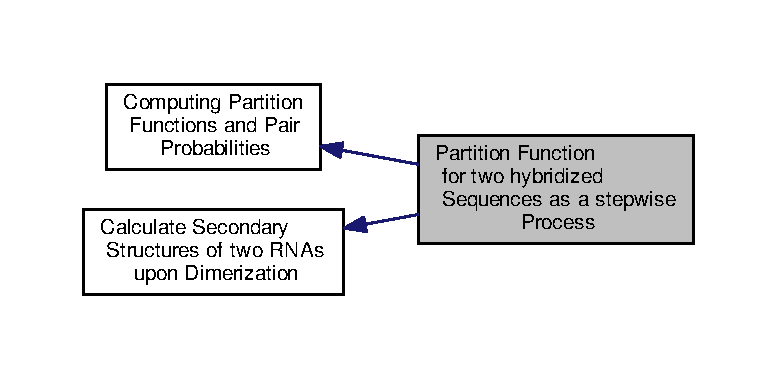
\includegraphics[width=350pt]{group__up__cofold}
\end{center}
\end{figure}
\subsection*{Files}
\begin{DoxyCompactItemize}
\item 
file \hyperlink{part__func__up_8h}{part\+\_\+func\+\_\+up.\+h}
\begin{DoxyCompactList}\small\item\em Partition Function Cofolding as stepwise process. \end{DoxyCompactList}\end{DoxyCompactItemize}
\subsection*{Functions}
\begin{DoxyCompactItemize}
\item 
\hyperlink{group__data__structures_structpu__contrib}{pu\+\_\+contrib} $\ast$ \hyperlink{group__up__cofold_ga5b4ee40e190d2f633cd01cf0d2fe93cf}{pf\+\_\+unstru} (char $\ast$sequence, int max\+\_\+w)
\begin{DoxyCompactList}\small\item\em Calculate the partition function over all unpaired regions of a maximal length. \end{DoxyCompactList}\item 
\hyperlink{group__data__structures_structinteract}{interact} $\ast$ \hyperlink{group__up__cofold_ga1aa0aa02bc3a724f87360c03097afd00}{pf\+\_\+interact} (const char $\ast$s1, const char $\ast$s2, \hyperlink{group__data__structures_structpu__contrib}{pu\+\_\+contrib} $\ast$p\+\_\+c, \hyperlink{group__data__structures_structpu__contrib}{pu\+\_\+contrib} $\ast$p\+\_\+c2, int max\+\_\+w, char $\ast$cstruc, int incr3, int incr5)
\begin{DoxyCompactList}\small\item\em Calculates the probability of a local interaction between two sequences. \end{DoxyCompactList}\item 
\hypertarget{group__up__cofold_gadde308fd5f696dc271b1532aa96fd12f}{}void \hyperlink{group__up__cofold_gadde308fd5f696dc271b1532aa96fd12f}{free\+\_\+interact} (\hyperlink{group__data__structures_structinteract}{interact} $\ast$pin)\label{group__up__cofold_gadde308fd5f696dc271b1532aa96fd12f}

\begin{DoxyCompactList}\small\item\em Frees the output of function \hyperlink{group__up__cofold_ga1aa0aa02bc3a724f87360c03097afd00}{pf\+\_\+interact()}. \end{DoxyCompactList}\item 
\hypertarget{group__up__cofold_gac20bd61824981d45ce0dc9934aa56df8}{}void \hyperlink{group__up__cofold_gac20bd61824981d45ce0dc9934aa56df8}{free\+\_\+pu\+\_\+contrib\+\_\+struct} (\hyperlink{group__data__structures_structpu__contrib}{pu\+\_\+contrib} $\ast$pu)\label{group__up__cofold_gac20bd61824981d45ce0dc9934aa56df8}

\begin{DoxyCompactList}\small\item\em Frees the output of function \hyperlink{group__up__cofold_ga5b4ee40e190d2f633cd01cf0d2fe93cf}{pf\+\_\+unstru()}. \end{DoxyCompactList}\end{DoxyCompactItemize}


\subsection{Detailed Description}
Partition Function Cofolding as a stepwise process. 



\subsection{Function Documentation}
\hypertarget{group__up__cofold_ga5b4ee40e190d2f633cd01cf0d2fe93cf}{}\index{Partition Function for two hybridized Sequences as a stepwise Process@{Partition Function for two hybridized Sequences as a stepwise Process}!pf\+\_\+unstru@{pf\+\_\+unstru}}
\index{pf\+\_\+unstru@{pf\+\_\+unstru}!Partition Function for two hybridized Sequences as a stepwise Process@{Partition Function for two hybridized Sequences as a stepwise Process}}
\subsubsection[{pf\+\_\+unstru}]{\setlength{\rightskip}{0pt plus 5cm}{\bf pu\+\_\+contrib}$\ast$ pf\+\_\+unstru (
\begin{DoxyParamCaption}
\item[{char $\ast$}]{sequence, }
\item[{int}]{max\+\_\+w}
\end{DoxyParamCaption}
)}\label{group__up__cofold_ga5b4ee40e190d2f633cd01cf0d2fe93cf}


{\ttfamily \#include $<$\hyperlink{part__func__up_8h}{Vienna\+R\+N\+A/part\+\_\+func\+\_\+up.\+h}$>$}



Calculate the partition function over all unpaired regions of a maximal length. 

You have to call function \hyperlink{group__pf__fold_gadc3db3d98742427e7001a7fd36ef28c2}{pf\+\_\+fold()} providing the same sequence before calling \hyperlink{group__up__cofold_ga5b4ee40e190d2f633cd01cf0d2fe93cf}{pf\+\_\+unstru()}. If you want to calculate unpaired regions for a constrained structure, set variable \textquotesingle{}structure\textquotesingle{} in function \textquotesingle{}\hyperlink{group__pf__fold_gadc3db3d98742427e7001a7fd36ef28c2}{pf\+\_\+fold()}\textquotesingle{} to the constrain string. It returns a \hyperlink{group__data__structures_structpu__contrib}{pu\+\_\+contrib} struct containing four arrays of dimension \mbox{[}i = 1 to length(sequence)\mbox{]}\mbox{[}j = 0 to u-\/1\mbox{]} containing all possible contributions to the probabilities of unpaired regions of maximum length u. Each array in \hyperlink{group__data__structures_structpu__contrib}{pu\+\_\+contrib} contains one of the contributions to the total probability of being unpaired\+: The probability of being unpaired within an exterior loop is in array \hyperlink{group__data__structures_structpu__contrib}{pu\+\_\+contrib}-\/$>$E, the probability of being unpaired within a hairpin loop is in array \hyperlink{group__data__structures_structpu__contrib}{pu\+\_\+contrib}-\/$>$H, the probability of being unpaired within an interior loop is in array \hyperlink{group__data__structures_structpu__contrib}{pu\+\_\+contrib}-\/$>$I and probability of being unpaired within a multi-\/loop is in array \hyperlink{group__data__structures_structpu__contrib}{pu\+\_\+contrib}-\/$>$M. The total probability of being unpaired is the sum of the four arrays of \hyperlink{group__data__structures_structpu__contrib}{pu\+\_\+contrib}.

This function frees everything allocated automatically. To free the output structure call free\+\_\+pu\+\_\+contrib().


\begin{DoxyParams}{Parameters}
{\em sequence} & \\
\hline
{\em max\+\_\+w} & \\
\hline
\end{DoxyParams}
\begin{DoxyReturn}{Returns}

\end{DoxyReturn}
\hypertarget{group__up__cofold_ga1aa0aa02bc3a724f87360c03097afd00}{}\index{Partition Function for two hybridized Sequences as a stepwise Process@{Partition Function for two hybridized Sequences as a stepwise Process}!pf\+\_\+interact@{pf\+\_\+interact}}
\index{pf\+\_\+interact@{pf\+\_\+interact}!Partition Function for two hybridized Sequences as a stepwise Process@{Partition Function for two hybridized Sequences as a stepwise Process}}
\subsubsection[{pf\+\_\+interact}]{\setlength{\rightskip}{0pt plus 5cm}{\bf interact}$\ast$ pf\+\_\+interact (
\begin{DoxyParamCaption}
\item[{const char $\ast$}]{s1, }
\item[{const char $\ast$}]{s2, }
\item[{{\bf pu\+\_\+contrib} $\ast$}]{p\+\_\+c, }
\item[{{\bf pu\+\_\+contrib} $\ast$}]{p\+\_\+c2, }
\item[{int}]{max\+\_\+w, }
\item[{char $\ast$}]{cstruc, }
\item[{int}]{incr3, }
\item[{int}]{incr5}
\end{DoxyParamCaption}
)}\label{group__up__cofold_ga1aa0aa02bc3a724f87360c03097afd00}


{\ttfamily \#include $<$\hyperlink{part__func__up_8h}{Vienna\+R\+N\+A/part\+\_\+func\+\_\+up.\+h}$>$}



Calculates the probability of a local interaction between two sequences. 

The function considers the probability that the region of interaction is unpaired within \textquotesingle{}s1\textquotesingle{} and \textquotesingle{}s2\textquotesingle{}. The longer sequence has to be given as \textquotesingle{}s1\textquotesingle{}. The shorter sequence has to be given as \textquotesingle{}s2\textquotesingle{}. Function \hyperlink{group__up__cofold_ga5b4ee40e190d2f633cd01cf0d2fe93cf}{pf\+\_\+unstru()} has to be called for \textquotesingle{}s1\textquotesingle{} and \textquotesingle{}s2\textquotesingle{}, where the probabilities of being unpaired have to be given in \textquotesingle{}p\+\_\+c\textquotesingle{} and \textquotesingle{}p\+\_\+c2\textquotesingle{}, respectively. If you do not want to include the probabilities of being unpaired for \textquotesingle{}s2\textquotesingle{} set \textquotesingle{}p\+\_\+c2\textquotesingle{} to N\+U\+L\+L. If variable \textquotesingle{}cstruc\textquotesingle{} is not N\+U\+L\+L, constrained folding is done\+: The available constrains for intermolecular interaction are\+: \textquotesingle{}.\textquotesingle{} (no constrain), \textquotesingle{}x\textquotesingle{} (the base has no intermolecular interaction) and \textquotesingle{}$\vert$\textquotesingle{} (the corresponding base has to be paired intermolecularily).~\newline
The parameter \textquotesingle{}w\textquotesingle{} determines the maximal length of the interaction. The parameters \textquotesingle{}incr5\textquotesingle{} and \textquotesingle{}incr3\textquotesingle{} allows inclusion of unpaired residues left (\textquotesingle{}incr5\textquotesingle{}) and right (\textquotesingle{}incr3\textquotesingle{}) of the region of interaction in \textquotesingle{}s1\textquotesingle{}. If the \textquotesingle{}incr\textquotesingle{} options are used, function \hyperlink{group__up__cofold_ga5b4ee40e190d2f633cd01cf0d2fe93cf}{pf\+\_\+unstru()} has to be called with w=w+incr5+incr3 for the longer sequence \textquotesingle{}s1\textquotesingle{}.

It returns a structure of type \hyperlink{group__data__structures_structinteract}{interact} which contains the probability of the best local interaction including residue i in Pi and the minimum free energy in Gi, where i is the position in sequence \textquotesingle{}s1\textquotesingle{}. The member Gikjl of structure \hyperlink{group__data__structures_structinteract}{interact} is the best interaction between region \mbox{[}k,i\mbox{]} k$<$i in longer sequence \textquotesingle{}s1\textquotesingle{} and region \mbox{[}j,l\mbox{]} j$<$l in \textquotesingle{}s2\textquotesingle{}. Gikjl\+\_\+wo is Gikjl without the probability of beeing unpaired.~\newline
Use \hyperlink{group__up__cofold_gadde308fd5f696dc271b1532aa96fd12f}{free\+\_\+interact()} to free the returned structure, all other stuff is freed inside \hyperlink{group__up__cofold_ga1aa0aa02bc3a724f87360c03097afd00}{pf\+\_\+interact()}.


\begin{DoxyParams}{Parameters}
{\em s1} & \\
\hline
{\em s2} & \\
\hline
{\em p\+\_\+c} & \\
\hline
{\em p\+\_\+c2} & \\
\hline
{\em max\+\_\+w} & \\
\hline
{\em cstruc} & \\
\hline
{\em incr3} & \\
\hline
{\em incr5} & \\
\hline
\end{DoxyParams}
\begin{DoxyReturn}{Returns}

\end{DoxyReturn}

\include{group__consensus__fold}
\include{group__consensus__mfe__fold}
\include{group__consensus__pf__fold}
\include{group__consensus__stochbt}
\include{group__local__fold}
\include{group__local__mfe__fold}
\hypertarget{group__local__pf__fold}{\section{Partition functions for locally stable secondary structures}
\label{group__local__pf__fold}\index{Partition functions for locally stable secondary structures@{Partition functions for locally stable secondary structures}}
}
Collaboration diagram for Partition functions for locally stable secondary structures\+:
\nopagebreak
\begin{figure}[H]
\begin{center}
\leavevmode
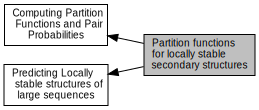
\includegraphics[width=331pt]{group__local__pf__fold}
\end{center}
\end{figure}
\subsection*{Files}
\begin{DoxyCompactItemize}
\item 
file \hyperlink{LPfold_8h}{L\+Pfold.\+h}
\begin{DoxyCompactList}\small\item\em Function declarations of partition function variants of the Lfold algorithm. \end{DoxyCompactList}\end{DoxyCompactItemize}
\subsection*{Functions}
\begin{DoxyCompactItemize}
\item 
void \hyperlink{group__local__pf__fold_ga5a019014d37fe6105131dfc2fc447880}{update\+\_\+pf\+\_\+params\+L\+P} (int length)
\item 
\hyperlink{group__data__structures_gab1d8894b43aa84cbc50b862a73785fbc}{plist} $\ast$ \hyperlink{group__local__pf__fold_ga7dcf599d07258801ea55e7d14a56908d}{pfl\+\_\+fold} (char $\ast$sequence, int win\+Size, int pair\+Size, float cutoffb, double $\ast$$\ast$p\+U, \hyperlink{group__data__structures_gab1d8894b43aa84cbc50b862a73785fbc}{plist} $\ast$$\ast$dpp2, F\+I\+L\+E $\ast$p\+Ufp, F\+I\+L\+E $\ast$spup)
\begin{DoxyCompactList}\small\item\em Compute partition functions for locally stable secondary structures. \end{DoxyCompactList}\item 
\hypertarget{group__local__pf__fold_ga14c2b82fdd5ab7a1951f1c2db4f5cf2c}{\hyperlink{group__data__structures_gab1d8894b43aa84cbc50b862a73785fbc}{plist} $\ast$ \hyperlink{group__local__pf__fold_ga14c2b82fdd5ab7a1951f1c2db4f5cf2c}{pfl\+\_\+fold\+\_\+par} (char $\ast$sequence, int win\+Size, int pair\+Size, float cutoffb, double $\ast$$\ast$p\+U, \hyperlink{group__data__structures_gab1d8894b43aa84cbc50b862a73785fbc}{plist} $\ast$$\ast$dpp2, F\+I\+L\+E $\ast$p\+Ufp, F\+I\+L\+E $\ast$spup, \hyperlink{group__energy__parameters_ga01d8b92fe734df8d79a6169482c7d8d8}{vrna\+\_\+exp\+\_\+param\+\_\+t} $\ast$parameters)}\label{group__local__pf__fold_ga14c2b82fdd5ab7a1951f1c2db4f5cf2c}

\begin{DoxyCompactList}\small\item\em Compute partition functions for locally stable secondary structures. \end{DoxyCompactList}\item 
void \hyperlink{group__local__pf__fold_ga0bcb751860bbf34e3dfee8c2fbdb3ef3}{putoutp\+U\+\_\+prob} (double $\ast$$\ast$p\+U, int length, int ulength, F\+I\+L\+E $\ast$fp, int energies)
\begin{DoxyCompactList}\small\item\em Writes the unpaired probabilities (p\+U) or opening energies into a file. \end{DoxyCompactList}\item 
void \hyperlink{group__local__pf__fold_ga9acb00ee10e96b1ca4ea394cd8bcec75}{putoutp\+U\+\_\+prob\+\_\+bin} (double $\ast$$\ast$p\+U, int length, int ulength, F\+I\+L\+E $\ast$fp, int energies)
\begin{DoxyCompactList}\small\item\em Writes the unpaired probabilities (p\+U) or opening energies into a binary file. \end{DoxyCompactList}\end{DoxyCompactItemize}


\subsection{Detailed Description}


\subsection{Function Documentation}
\hypertarget{group__local__pf__fold_ga5a019014d37fe6105131dfc2fc447880}{\index{Partition functions for locally stable secondary structures@{Partition functions for locally stable secondary structures}!update\+\_\+pf\+\_\+params\+L\+P@{update\+\_\+pf\+\_\+params\+L\+P}}
\index{update\+\_\+pf\+\_\+params\+L\+P@{update\+\_\+pf\+\_\+params\+L\+P}!Partition functions for locally stable secondary structures@{Partition functions for locally stable secondary structures}}
\subsubsection[{update\+\_\+pf\+\_\+params\+L\+P}]{\setlength{\rightskip}{0pt plus 5cm}void update\+\_\+pf\+\_\+params\+L\+P (
\begin{DoxyParamCaption}
\item[{int}]{length}
\end{DoxyParamCaption}
)}}\label{group__local__pf__fold_ga5a019014d37fe6105131dfc2fc447880}


{\ttfamily \#include $<$\hyperlink{LPfold_8h}{Vienna\+R\+N\+A/\+L\+Pfold.\+h}$>$}


\begin{DoxyParams}{Parameters}
{\em length} & \\
\hline
\end{DoxyParams}
\hypertarget{group__local__pf__fold_ga7dcf599d07258801ea55e7d14a56908d}{\index{Partition functions for locally stable secondary structures@{Partition functions for locally stable secondary structures}!pfl\+\_\+fold@{pfl\+\_\+fold}}
\index{pfl\+\_\+fold@{pfl\+\_\+fold}!Partition functions for locally stable secondary structures@{Partition functions for locally stable secondary structures}}
\subsubsection[{pfl\+\_\+fold}]{\setlength{\rightskip}{0pt plus 5cm}{\bf plist}$\ast$ pfl\+\_\+fold (
\begin{DoxyParamCaption}
\item[{char $\ast$}]{sequence, }
\item[{int}]{win\+Size, }
\item[{int}]{pair\+Size, }
\item[{float}]{cutoffb, }
\item[{double $\ast$$\ast$}]{p\+U, }
\item[{{\bf plist} $\ast$$\ast$}]{dpp2, }
\item[{F\+I\+L\+E $\ast$}]{p\+Ufp, }
\item[{F\+I\+L\+E $\ast$}]{spup}
\end{DoxyParamCaption}
)}}\label{group__local__pf__fold_ga7dcf599d07258801ea55e7d14a56908d}


{\ttfamily \#include $<$\hyperlink{LPfold_8h}{Vienna\+R\+N\+A/\+L\+Pfold.\+h}$>$}



Compute partition functions for locally stable secondary structures. 

pfl\+\_\+fold computes partition functions for every window of size 'win\+Size' possible in a R\+N\+A molecule, allowing only pairs with a span smaller than 'pair\+Size'. It returns the mean pair probabilities averaged over all windows containing the pair in 'pl'. 'win\+Size' should always be $>$= 'pair\+Size'. Note that in contrast to \hyperlink{group__local__mfe__fold_ga16e5a70e60835bb969eaecbe6482f1be}{Lfold()}, bases outside of the window do not influence the structure at all. Only probabilities higher than 'cutoffb' are kept.

If 'p\+U' is supplied (i.\+e is not the N\+U\+L\+L pointer), \hyperlink{group__local__pf__fold_ga7dcf599d07258801ea55e7d14a56908d}{pfl\+\_\+fold()} will also compute the mean probability that regions of length 'u' and smaller are unpaired. The parameter 'u' is supplied in 'pup\mbox{[}0\mbox{]}\mbox{[}0\mbox{]}'. On return the 'pup' array will contain these probabilities, with the entry on 'pup\mbox{[}x\mbox{]}\mbox{[}y\mbox{]}' containing the mean probability that x and the y-\/1 preceding bases are unpaired. The 'p\+U' array needs to be large enough to hold n+1 float$\ast$ entries, where n is the sequence length.

If an array dpp2 is supplied, the probability of base pair (i,j) given that there already exists a base pair (i+1,j-\/1) is also computed and saved in this array. If p\+Ufp is given (i.\+e. not N\+U\+L\+L), p\+U is not saved but put out imediately. If spup is given (i.\+e. is not N\+U\+L\+L), the pair probabilities in pl are not saved but put out imediately.


\begin{DoxyParams}{Parameters}
{\em sequence} & R\+N\+A sequence \\
\hline
{\em win\+Size} & size of the window \\
\hline
{\em pair\+Size} & maximum size of base pair \\
\hline
{\em cutoffb} & cutoffb for base pairs \\
\hline
{\em p\+U} & array holding all unpaired probabilities \\
\hline
{\em dpp2} & array of dependent pair probabilities \\
\hline
{\em p\+Ufp} & file pointer for p\+U \\
\hline
{\em spup} & file pointer for pair probabilities \\
\hline
\end{DoxyParams}
\begin{DoxyReturn}{Returns}
list of pair probabilities 
\end{DoxyReturn}
\hypertarget{group__local__pf__fold_ga0bcb751860bbf34e3dfee8c2fbdb3ef3}{\index{Partition functions for locally stable secondary structures@{Partition functions for locally stable secondary structures}!putoutp\+U\+\_\+prob@{putoutp\+U\+\_\+prob}}
\index{putoutp\+U\+\_\+prob@{putoutp\+U\+\_\+prob}!Partition functions for locally stable secondary structures@{Partition functions for locally stable secondary structures}}
\subsubsection[{putoutp\+U\+\_\+prob}]{\setlength{\rightskip}{0pt plus 5cm}void putoutp\+U\+\_\+prob (
\begin{DoxyParamCaption}
\item[{double $\ast$$\ast$}]{p\+U, }
\item[{int}]{length, }
\item[{int}]{ulength, }
\item[{F\+I\+L\+E $\ast$}]{fp, }
\item[{int}]{energies}
\end{DoxyParamCaption}
)}}\label{group__local__pf__fold_ga0bcb751860bbf34e3dfee8c2fbdb3ef3}


{\ttfamily \#include $<$\hyperlink{LPfold_8h}{Vienna\+R\+N\+A/\+L\+Pfold.\+h}$>$}



Writes the unpaired probabilities (p\+U) or opening energies into a file. 

Can write either the unpaired probabilities (accessibilities) p\+U or the opening energies -\/log(p\+U)k\+T into a file


\begin{DoxyParams}{Parameters}
{\em p\+U} & pair probabilities \\
\hline
{\em length} & length of R\+N\+A sequence \\
\hline
{\em ulength} & maximum length of unpaired stretch \\
\hline
{\em fp} & file pointer of destination file \\
\hline
{\em energies} & switch to put out as opening energies \\
\hline
\end{DoxyParams}
\hypertarget{group__local__pf__fold_ga9acb00ee10e96b1ca4ea394cd8bcec75}{\index{Partition functions for locally stable secondary structures@{Partition functions for locally stable secondary structures}!putoutp\+U\+\_\+prob\+\_\+bin@{putoutp\+U\+\_\+prob\+\_\+bin}}
\index{putoutp\+U\+\_\+prob\+\_\+bin@{putoutp\+U\+\_\+prob\+\_\+bin}!Partition functions for locally stable secondary structures@{Partition functions for locally stable secondary structures}}
\subsubsection[{putoutp\+U\+\_\+prob\+\_\+bin}]{\setlength{\rightskip}{0pt plus 5cm}void putoutp\+U\+\_\+prob\+\_\+bin (
\begin{DoxyParamCaption}
\item[{double $\ast$$\ast$}]{p\+U, }
\item[{int}]{length, }
\item[{int}]{ulength, }
\item[{F\+I\+L\+E $\ast$}]{fp, }
\item[{int}]{energies}
\end{DoxyParamCaption}
)}}\label{group__local__pf__fold_ga9acb00ee10e96b1ca4ea394cd8bcec75}


{\ttfamily \#include $<$\hyperlink{LPfold_8h}{Vienna\+R\+N\+A/\+L\+Pfold.\+h}$>$}



Writes the unpaired probabilities (p\+U) or opening energies into a binary file. 

Can write either the unpaired probabilities (accessibilities) p\+U or the opening energies -\/log(p\+U)k\+T into a file


\begin{DoxyParams}{Parameters}
{\em p\+U} & pair probabilities \\
\hline
{\em length} & length of R\+N\+A sequence \\
\hline
{\em ulength} & maximum length of unpaired stretch \\
\hline
{\em fp} & file pointer of destination file \\
\hline
{\em energies} & switch to put out as opening energies \\
\hline
\end{DoxyParams}

\hypertarget{group__local__consensus__fold}{}\section{Local M\+F\+E consensus structures for Sequence Alignments}
\label{group__local__consensus__fold}\index{Local M\+F\+E consensus structures for Sequence Alignments@{Local M\+F\+E consensus structures for Sequence Alignments}}
Collaboration diagram for Local M\+F\+E consensus structures for Sequence Alignments\+:
\nopagebreak
\begin{figure}[H]
\begin{center}
\leavevmode
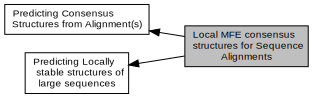
\includegraphics[width=350pt]{group__local__consensus__fold}
\end{center}
\end{figure}
\subsection*{Functions}
\begin{DoxyCompactItemize}
\item 
float \hyperlink{group__local__consensus__fold_ga20a173a3cdb83f5d1778e36c1a6b1f2b}{ali\+Lfold} (const char $\ast$$\ast$strings, char $\ast$structure, int maxdist)
\end{DoxyCompactItemize}


\subsection{Detailed Description}


\subsection{Function Documentation}
\hypertarget{group__local__consensus__fold_ga20a173a3cdb83f5d1778e36c1a6b1f2b}{}\index{Local M\+F\+E consensus structures for Sequence Alignments@{Local M\+F\+E consensus structures for Sequence Alignments}!ali\+Lfold@{ali\+Lfold}}
\index{ali\+Lfold@{ali\+Lfold}!Local M\+F\+E consensus structures for Sequence Alignments@{Local M\+F\+E consensus structures for Sequence Alignments}}
\subsubsection[{ali\+Lfold}]{\setlength{\rightskip}{0pt plus 5cm}float ali\+Lfold (
\begin{DoxyParamCaption}
\item[{const char $\ast$$\ast$}]{strings, }
\item[{char $\ast$}]{structure, }
\item[{int}]{maxdist}
\end{DoxyParamCaption}
)}\label{group__local__consensus__fold_ga20a173a3cdb83f5d1778e36c1a6b1f2b}


{\ttfamily \#include $<$\hyperlink{Lfold_8h}{Vienna\+R\+N\+A/\+Lfold.\+h}$>$}


\begin{DoxyParams}{Parameters}
{\em strings} & \\
\hline
{\em structure} & \\
\hline
{\em maxdist} & \\
\hline
\end{DoxyParams}
\begin{DoxyReturn}{Returns}

\end{DoxyReturn}

\hypertarget{group__energy__parameters__rw}{\section{Reading/\+Writing Energy Parameter Sets from/to File}
\label{group__energy__parameters__rw}\index{Reading/\+Writing Energy Parameter Sets from/to File@{Reading/\+Writing Energy Parameter Sets from/to File}}
}


Read and Write energy parameter sets from and to text files.  


Collaboration diagram for Reading/\+Writing Energy Parameter Sets from/to File\+:
\nopagebreak
\begin{figure}[H]
\begin{center}
\leavevmode
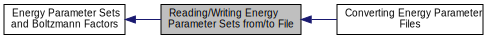
\includegraphics[width=350pt]{group__energy__parameters__rw}
\end{center}
\end{figure}
\subsection*{Modules}
\begin{DoxyCompactItemize}
\item 
\hyperlink{group__energy__parameters__convert}{Converting Energy Parameter Files}
\begin{DoxyCompactList}\small\item\em Convert energy parameter files into the latest format. \end{DoxyCompactList}\end{DoxyCompactItemize}
\subsection*{Files}
\begin{DoxyCompactItemize}
\item 
file \hyperlink{read__epars_8h}{read\+\_\+epars.\+h}
\end{DoxyCompactItemize}
\subsection*{Functions}
\begin{DoxyCompactItemize}
\item 
void \hyperlink{group__energy__parameters__rw_ga165a142a3c68fb6655c69ef4ab7cd749}{read\+\_\+parameter\+\_\+file} (const char fname\mbox{[}$\,$\mbox{]})
\begin{DoxyCompactList}\small\item\em Read energy parameters from a file. \end{DoxyCompactList}\item 
void \hyperlink{group__energy__parameters__rw_ga8a43459be386a7489feeab68dc2c6c76}{write\+\_\+parameter\+\_\+file} (const char fname\mbox{[}$\,$\mbox{]})
\begin{DoxyCompactList}\small\item\em Write energy parameters to a file. \end{DoxyCompactList}\end{DoxyCompactItemize}


\subsection{Detailed Description}
Read and Write energy parameter sets from and to text files. 

A default set of parameters, identical to the one described in \cite{mathews:2004} and \cite{turner:2010}, is compiled into the library. 

\subsection{Function Documentation}
\hypertarget{group__energy__parameters__rw_ga165a142a3c68fb6655c69ef4ab7cd749}{\index{Reading/\+Writing Energy Parameter Sets from/to File@{Reading/\+Writing Energy Parameter Sets from/to File}!read\+\_\+parameter\+\_\+file@{read\+\_\+parameter\+\_\+file}}
\index{read\+\_\+parameter\+\_\+file@{read\+\_\+parameter\+\_\+file}!Reading/\+Writing Energy Parameter Sets from/to File@{Reading/\+Writing Energy Parameter Sets from/to File}}
\subsubsection[{read\+\_\+parameter\+\_\+file}]{\setlength{\rightskip}{0pt plus 5cm}void read\+\_\+parameter\+\_\+file (
\begin{DoxyParamCaption}
\item[{const char}]{fname\mbox{[}$\,$\mbox{]}}
\end{DoxyParamCaption}
)}}\label{group__energy__parameters__rw_ga165a142a3c68fb6655c69ef4ab7cd749}


{\ttfamily \#include $<$\hyperlink{read__epars_8h}{Vienna\+R\+N\+A/read\+\_\+epars.\+h}$>$}



Read energy parameters from a file. 


\begin{DoxyParams}{Parameters}
{\em fname} & The path to the file containing the energy parameters \\
\hline
\end{DoxyParams}
\hypertarget{group__energy__parameters__rw_ga8a43459be386a7489feeab68dc2c6c76}{\index{Reading/\+Writing Energy Parameter Sets from/to File@{Reading/\+Writing Energy Parameter Sets from/to File}!write\+\_\+parameter\+\_\+file@{write\+\_\+parameter\+\_\+file}}
\index{write\+\_\+parameter\+\_\+file@{write\+\_\+parameter\+\_\+file}!Reading/\+Writing Energy Parameter Sets from/to File@{Reading/\+Writing Energy Parameter Sets from/to File}}
\subsubsection[{write\+\_\+parameter\+\_\+file}]{\setlength{\rightskip}{0pt plus 5cm}void write\+\_\+parameter\+\_\+file (
\begin{DoxyParamCaption}
\item[{const char}]{fname\mbox{[}$\,$\mbox{]}}
\end{DoxyParamCaption}
)}}\label{group__energy__parameters__rw_ga8a43459be386a7489feeab68dc2c6c76}


{\ttfamily \#include $<$\hyperlink{read__epars_8h}{Vienna\+R\+N\+A/read\+\_\+epars.\+h}$>$}



Write energy parameters to a file. 


\begin{DoxyParams}{Parameters}
{\em fname} & A filename (path) for the file where the current energy parameters will be written to \\
\hline
\end{DoxyParams}

\hypertarget{group__energy__parameters__convert}{\section{Converting Energy Parameter Files}
\label{group__energy__parameters__convert}\index{Converting Energy Parameter Files@{Converting Energy Parameter Files}}
}


Convert energy parameter files into the latest format.  


Collaboration diagram for Converting Energy Parameter Files\+:
\nopagebreak
\begin{figure}[H]
\begin{center}
\leavevmode
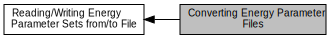
\includegraphics[width=350pt]{group__energy__parameters__convert}
\end{center}
\end{figure}
\subsection*{Files}
\begin{DoxyCompactItemize}
\item 
file \hyperlink{convert__epars_8h}{convert\+\_\+epars.\+h}
\begin{DoxyCompactList}\small\item\em Functions and definitions for energy parameter file format conversion. \end{DoxyCompactList}\end{DoxyCompactItemize}
\subsection*{Macros}
\begin{DoxyCompactItemize}
\item 
\#define \hyperlink{group__energy__parameters__convert_ga8dc6aee5a806c49b71557152f9616bc4}{V\+R\+N\+A\+\_\+\+C\+O\+N\+V\+E\+R\+T\+\_\+\+O\+U\+T\+P\+U\+T\+\_\+\+A\+L\+L}~1\+U
\item 
\#define \hyperlink{group__energy__parameters__convert_gaf66fe2cb11dfcfd32d791049c254a8a4}{V\+R\+N\+A\+\_\+\+C\+O\+N\+V\+E\+R\+T\+\_\+\+O\+U\+T\+P\+U\+T\+\_\+\+H\+P}~2\+U
\item 
\#define \hyperlink{group__energy__parameters__convert_gad23522d63f8d4c50d5a5deee9bee3ef2}{V\+R\+N\+A\+\_\+\+C\+O\+N\+V\+E\+R\+T\+\_\+\+O\+U\+T\+P\+U\+T\+\_\+\+S\+T\+A\+C\+K}~4\+U
\item 
\#define \hyperlink{group__energy__parameters__convert_gaa892c7b4957459090f3e08da298cc347}{V\+R\+N\+A\+\_\+\+C\+O\+N\+V\+E\+R\+T\+\_\+\+O\+U\+T\+P\+U\+T\+\_\+\+M\+M\+\_\+\+H\+P}~8\+U
\item 
\#define \hyperlink{group__energy__parameters__convert_ga4ff223fb1f9c62cd92d9ab811ad03d55}{V\+R\+N\+A\+\_\+\+C\+O\+N\+V\+E\+R\+T\+\_\+\+O\+U\+T\+P\+U\+T\+\_\+\+M\+M\+\_\+\+I\+N\+T}~16\+U
\item 
\#define \hyperlink{group__energy__parameters__convert_gaf5d3743219f83c6348155cd81e755bbb}{V\+R\+N\+A\+\_\+\+C\+O\+N\+V\+E\+R\+T\+\_\+\+O\+U\+T\+P\+U\+T\+\_\+\+M\+M\+\_\+\+I\+N\+T\+\_\+1\+N}~32\+U
\item 
\#define \hyperlink{group__energy__parameters__convert_ga78382ec622ba99e0ac2262317bdd7316}{V\+R\+N\+A\+\_\+\+C\+O\+N\+V\+E\+R\+T\+\_\+\+O\+U\+T\+P\+U\+T\+\_\+\+M\+M\+\_\+\+I\+N\+T\+\_\+23}~64\+U
\item 
\#define \hyperlink{group__energy__parameters__convert_gae67af9f1cdf7baf2865481282a5d1034}{V\+R\+N\+A\+\_\+\+C\+O\+N\+V\+E\+R\+T\+\_\+\+O\+U\+T\+P\+U\+T\+\_\+\+M\+M\+\_\+\+M\+U\+L\+T\+I}~128\+U
\item 
\#define \hyperlink{group__energy__parameters__convert_gaf14ead7ef1fdbe725ade653750fc51e3}{V\+R\+N\+A\+\_\+\+C\+O\+N\+V\+E\+R\+T\+\_\+\+O\+U\+T\+P\+U\+T\+\_\+\+M\+M\+\_\+\+E\+X\+T}~256\+U
\item 
\#define \hyperlink{group__energy__parameters__convert_ga036ffd996d8c8a9acf631760dd1da24b}{V\+R\+N\+A\+\_\+\+C\+O\+N\+V\+E\+R\+T\+\_\+\+O\+U\+T\+P\+U\+T\+\_\+\+D\+A\+N\+G\+L\+E5}~512\+U
\item 
\#define \hyperlink{group__energy__parameters__convert_ga34a8a5479ef885834ef32f3fb43d79bc}{V\+R\+N\+A\+\_\+\+C\+O\+N\+V\+E\+R\+T\+\_\+\+O\+U\+T\+P\+U\+T\+\_\+\+D\+A\+N\+G\+L\+E3}~1024\+U
\item 
\#define \hyperlink{group__energy__parameters__convert_ga079aafefd5f8ab57ee5120099a34bd25}{V\+R\+N\+A\+\_\+\+C\+O\+N\+V\+E\+R\+T\+\_\+\+O\+U\+T\+P\+U\+T\+\_\+\+I\+N\+T\+\_\+11}~2048\+U
\item 
\#define \hyperlink{group__energy__parameters__convert_gacf770881d9034431ebe741642342a1f9}{V\+R\+N\+A\+\_\+\+C\+O\+N\+V\+E\+R\+T\+\_\+\+O\+U\+T\+P\+U\+T\+\_\+\+I\+N\+T\+\_\+21}~4096\+U
\item 
\#define \hyperlink{group__energy__parameters__convert_gaa307671e2631cdacad9cbe4c6583b05f}{V\+R\+N\+A\+\_\+\+C\+O\+N\+V\+E\+R\+T\+\_\+\+O\+U\+T\+P\+U\+T\+\_\+\+I\+N\+T\+\_\+22}~8192\+U
\item 
\#define \hyperlink{group__energy__parameters__convert_ga7092fe0be4de6f02cc0bf08e81af726a}{V\+R\+N\+A\+\_\+\+C\+O\+N\+V\+E\+R\+T\+\_\+\+O\+U\+T\+P\+U\+T\+\_\+\+B\+U\+L\+G\+E}~16384\+U
\item 
\#define \hyperlink{group__energy__parameters__convert_gac5c2289fdf8ff1b980976d1613ff943a}{V\+R\+N\+A\+\_\+\+C\+O\+N\+V\+E\+R\+T\+\_\+\+O\+U\+T\+P\+U\+T\+\_\+\+I\+N\+T}~32768\+U
\item 
\#define \hyperlink{group__energy__parameters__convert_gaf2c8755d64eff3852aa45df9ac80a4fe}{V\+R\+N\+A\+\_\+\+C\+O\+N\+V\+E\+R\+T\+\_\+\+O\+U\+T\+P\+U\+T\+\_\+\+M\+L}~65536\+U
\item 
\#define \hyperlink{group__energy__parameters__convert_ga46d5b1535ae86060b6317565b7c6b40b}{V\+R\+N\+A\+\_\+\+C\+O\+N\+V\+E\+R\+T\+\_\+\+O\+U\+T\+P\+U\+T\+\_\+\+M\+I\+S\+C}~131072\+U
\item 
\#define \hyperlink{group__energy__parameters__convert_gaa1ff48a79642d69579d1766561ec6db6}{V\+R\+N\+A\+\_\+\+C\+O\+N\+V\+E\+R\+T\+\_\+\+O\+U\+T\+P\+U\+T\+\_\+\+S\+P\+E\+C\+I\+A\+L\+\_\+\+H\+P}~262144\+U
\item 
\#define \hyperlink{group__energy__parameters__convert_ga0d4e8a836bb4864ab5129c085dbf592d}{V\+R\+N\+A\+\_\+\+C\+O\+N\+V\+E\+R\+T\+\_\+\+O\+U\+T\+P\+U\+T\+\_\+\+V\+A\+N\+I\+L\+L\+A}~524288\+U
\item 
\#define \hyperlink{group__energy__parameters__convert_ga2eb0462f16939ddacdaf751a88d675ce}{V\+R\+N\+A\+\_\+\+C\+O\+N\+V\+E\+R\+T\+\_\+\+O\+U\+T\+P\+U\+T\+\_\+\+N\+I\+N\+I\+O}~1048576\+U
\item 
\#define \hyperlink{group__energy__parameters__convert_gac86976e9c2a55b3a6481ea60044f6098}{V\+R\+N\+A\+\_\+\+C\+O\+N\+V\+E\+R\+T\+\_\+\+O\+U\+T\+P\+U\+T\+\_\+\+D\+U\+M\+P}~2097152\+U
\end{DoxyCompactItemize}
\subsection*{Functions}
\begin{DoxyCompactItemize}
\item 
void \hyperlink{group__energy__parameters__convert_gafbe538bc4eb2cf2a33326e1010005f8a}{convert\+\_\+parameter\+\_\+file} (const char $\ast$iname, const char $\ast$oname, unsigned int options)
\end{DoxyCompactItemize}


\subsection{Detailed Description}
Convert energy parameter files into the latest format. 

To preserve some backward compatibility the R\+N\+Alib also provides functions to convert energy parameter files from the format used in version 1.\+4-\/1.\+8 into the new format used since version 2.\+0 

\subsection{Macro Definition Documentation}
\hypertarget{group__energy__parameters__convert_ga8dc6aee5a806c49b71557152f9616bc4}{\index{Converting Energy Parameter Files@{Converting Energy Parameter Files}!V\+R\+N\+A\+\_\+\+C\+O\+N\+V\+E\+R\+T\+\_\+\+O\+U\+T\+P\+U\+T\+\_\+\+A\+L\+L@{V\+R\+N\+A\+\_\+\+C\+O\+N\+V\+E\+R\+T\+\_\+\+O\+U\+T\+P\+U\+T\+\_\+\+A\+L\+L}}
\index{V\+R\+N\+A\+\_\+\+C\+O\+N\+V\+E\+R\+T\+\_\+\+O\+U\+T\+P\+U\+T\+\_\+\+A\+L\+L@{V\+R\+N\+A\+\_\+\+C\+O\+N\+V\+E\+R\+T\+\_\+\+O\+U\+T\+P\+U\+T\+\_\+\+A\+L\+L}!Converting Energy Parameter Files@{Converting Energy Parameter Files}}
\subsubsection[{V\+R\+N\+A\+\_\+\+C\+O\+N\+V\+E\+R\+T\+\_\+\+O\+U\+T\+P\+U\+T\+\_\+\+A\+L\+L}]{\setlength{\rightskip}{0pt plus 5cm}\#define V\+R\+N\+A\+\_\+\+C\+O\+N\+V\+E\+R\+T\+\_\+\+O\+U\+T\+P\+U\+T\+\_\+\+A\+L\+L~1\+U}}\label{group__energy__parameters__convert_ga8dc6aee5a806c49b71557152f9616bc4}


{\ttfamily \#include $<$\hyperlink{convert__epars_8h}{Vienna\+R\+N\+A/convert\+\_\+epars.\+h}$>$}

Flag to indicate printing of a complete parameter set \hypertarget{group__energy__parameters__convert_gaf66fe2cb11dfcfd32d791049c254a8a4}{\index{Converting Energy Parameter Files@{Converting Energy Parameter Files}!V\+R\+N\+A\+\_\+\+C\+O\+N\+V\+E\+R\+T\+\_\+\+O\+U\+T\+P\+U\+T\+\_\+\+H\+P@{V\+R\+N\+A\+\_\+\+C\+O\+N\+V\+E\+R\+T\+\_\+\+O\+U\+T\+P\+U\+T\+\_\+\+H\+P}}
\index{V\+R\+N\+A\+\_\+\+C\+O\+N\+V\+E\+R\+T\+\_\+\+O\+U\+T\+P\+U\+T\+\_\+\+H\+P@{V\+R\+N\+A\+\_\+\+C\+O\+N\+V\+E\+R\+T\+\_\+\+O\+U\+T\+P\+U\+T\+\_\+\+H\+P}!Converting Energy Parameter Files@{Converting Energy Parameter Files}}
\subsubsection[{V\+R\+N\+A\+\_\+\+C\+O\+N\+V\+E\+R\+T\+\_\+\+O\+U\+T\+P\+U\+T\+\_\+\+H\+P}]{\setlength{\rightskip}{0pt plus 5cm}\#define V\+R\+N\+A\+\_\+\+C\+O\+N\+V\+E\+R\+T\+\_\+\+O\+U\+T\+P\+U\+T\+\_\+\+H\+P~2\+U}}\label{group__energy__parameters__convert_gaf66fe2cb11dfcfd32d791049c254a8a4}


{\ttfamily \#include $<$\hyperlink{convert__epars_8h}{Vienna\+R\+N\+A/convert\+\_\+epars.\+h}$>$}

Flag to indicate printing of hairpin contributions \hypertarget{group__energy__parameters__convert_gad23522d63f8d4c50d5a5deee9bee3ef2}{\index{Converting Energy Parameter Files@{Converting Energy Parameter Files}!V\+R\+N\+A\+\_\+\+C\+O\+N\+V\+E\+R\+T\+\_\+\+O\+U\+T\+P\+U\+T\+\_\+\+S\+T\+A\+C\+K@{V\+R\+N\+A\+\_\+\+C\+O\+N\+V\+E\+R\+T\+\_\+\+O\+U\+T\+P\+U\+T\+\_\+\+S\+T\+A\+C\+K}}
\index{V\+R\+N\+A\+\_\+\+C\+O\+N\+V\+E\+R\+T\+\_\+\+O\+U\+T\+P\+U\+T\+\_\+\+S\+T\+A\+C\+K@{V\+R\+N\+A\+\_\+\+C\+O\+N\+V\+E\+R\+T\+\_\+\+O\+U\+T\+P\+U\+T\+\_\+\+S\+T\+A\+C\+K}!Converting Energy Parameter Files@{Converting Energy Parameter Files}}
\subsubsection[{V\+R\+N\+A\+\_\+\+C\+O\+N\+V\+E\+R\+T\+\_\+\+O\+U\+T\+P\+U\+T\+\_\+\+S\+T\+A\+C\+K}]{\setlength{\rightskip}{0pt plus 5cm}\#define V\+R\+N\+A\+\_\+\+C\+O\+N\+V\+E\+R\+T\+\_\+\+O\+U\+T\+P\+U\+T\+\_\+\+S\+T\+A\+C\+K~4\+U}}\label{group__energy__parameters__convert_gad23522d63f8d4c50d5a5deee9bee3ef2}


{\ttfamily \#include $<$\hyperlink{convert__epars_8h}{Vienna\+R\+N\+A/convert\+\_\+epars.\+h}$>$}

Flag to indicate printing of base pair stack contributions \hypertarget{group__energy__parameters__convert_gaa892c7b4957459090f3e08da298cc347}{\index{Converting Energy Parameter Files@{Converting Energy Parameter Files}!V\+R\+N\+A\+\_\+\+C\+O\+N\+V\+E\+R\+T\+\_\+\+O\+U\+T\+P\+U\+T\+\_\+\+M\+M\+\_\+\+H\+P@{V\+R\+N\+A\+\_\+\+C\+O\+N\+V\+E\+R\+T\+\_\+\+O\+U\+T\+P\+U\+T\+\_\+\+M\+M\+\_\+\+H\+P}}
\index{V\+R\+N\+A\+\_\+\+C\+O\+N\+V\+E\+R\+T\+\_\+\+O\+U\+T\+P\+U\+T\+\_\+\+M\+M\+\_\+\+H\+P@{V\+R\+N\+A\+\_\+\+C\+O\+N\+V\+E\+R\+T\+\_\+\+O\+U\+T\+P\+U\+T\+\_\+\+M\+M\+\_\+\+H\+P}!Converting Energy Parameter Files@{Converting Energy Parameter Files}}
\subsubsection[{V\+R\+N\+A\+\_\+\+C\+O\+N\+V\+E\+R\+T\+\_\+\+O\+U\+T\+P\+U\+T\+\_\+\+M\+M\+\_\+\+H\+P}]{\setlength{\rightskip}{0pt plus 5cm}\#define V\+R\+N\+A\+\_\+\+C\+O\+N\+V\+E\+R\+T\+\_\+\+O\+U\+T\+P\+U\+T\+\_\+\+M\+M\+\_\+\+H\+P~8\+U}}\label{group__energy__parameters__convert_gaa892c7b4957459090f3e08da298cc347}


{\ttfamily \#include $<$\hyperlink{convert__epars_8h}{Vienna\+R\+N\+A/convert\+\_\+epars.\+h}$>$}

Flag to indicate printing of hairpin mismatch contribution \hypertarget{group__energy__parameters__convert_ga4ff223fb1f9c62cd92d9ab811ad03d55}{\index{Converting Energy Parameter Files@{Converting Energy Parameter Files}!V\+R\+N\+A\+\_\+\+C\+O\+N\+V\+E\+R\+T\+\_\+\+O\+U\+T\+P\+U\+T\+\_\+\+M\+M\+\_\+\+I\+N\+T@{V\+R\+N\+A\+\_\+\+C\+O\+N\+V\+E\+R\+T\+\_\+\+O\+U\+T\+P\+U\+T\+\_\+\+M\+M\+\_\+\+I\+N\+T}}
\index{V\+R\+N\+A\+\_\+\+C\+O\+N\+V\+E\+R\+T\+\_\+\+O\+U\+T\+P\+U\+T\+\_\+\+M\+M\+\_\+\+I\+N\+T@{V\+R\+N\+A\+\_\+\+C\+O\+N\+V\+E\+R\+T\+\_\+\+O\+U\+T\+P\+U\+T\+\_\+\+M\+M\+\_\+\+I\+N\+T}!Converting Energy Parameter Files@{Converting Energy Parameter Files}}
\subsubsection[{V\+R\+N\+A\+\_\+\+C\+O\+N\+V\+E\+R\+T\+\_\+\+O\+U\+T\+P\+U\+T\+\_\+\+M\+M\+\_\+\+I\+N\+T}]{\setlength{\rightskip}{0pt plus 5cm}\#define V\+R\+N\+A\+\_\+\+C\+O\+N\+V\+E\+R\+T\+\_\+\+O\+U\+T\+P\+U\+T\+\_\+\+M\+M\+\_\+\+I\+N\+T~16\+U}}\label{group__energy__parameters__convert_ga4ff223fb1f9c62cd92d9ab811ad03d55}


{\ttfamily \#include $<$\hyperlink{convert__epars_8h}{Vienna\+R\+N\+A/convert\+\_\+epars.\+h}$>$}

Flag to indicate printing of interior loop mismatch contribution \hypertarget{group__energy__parameters__convert_gaf5d3743219f83c6348155cd81e755bbb}{\index{Converting Energy Parameter Files@{Converting Energy Parameter Files}!V\+R\+N\+A\+\_\+\+C\+O\+N\+V\+E\+R\+T\+\_\+\+O\+U\+T\+P\+U\+T\+\_\+\+M\+M\+\_\+\+I\+N\+T\+\_\+1\+N@{V\+R\+N\+A\+\_\+\+C\+O\+N\+V\+E\+R\+T\+\_\+\+O\+U\+T\+P\+U\+T\+\_\+\+M\+M\+\_\+\+I\+N\+T\+\_\+1\+N}}
\index{V\+R\+N\+A\+\_\+\+C\+O\+N\+V\+E\+R\+T\+\_\+\+O\+U\+T\+P\+U\+T\+\_\+\+M\+M\+\_\+\+I\+N\+T\+\_\+1\+N@{V\+R\+N\+A\+\_\+\+C\+O\+N\+V\+E\+R\+T\+\_\+\+O\+U\+T\+P\+U\+T\+\_\+\+M\+M\+\_\+\+I\+N\+T\+\_\+1\+N}!Converting Energy Parameter Files@{Converting Energy Parameter Files}}
\subsubsection[{V\+R\+N\+A\+\_\+\+C\+O\+N\+V\+E\+R\+T\+\_\+\+O\+U\+T\+P\+U\+T\+\_\+\+M\+M\+\_\+\+I\+N\+T\+\_\+1\+N}]{\setlength{\rightskip}{0pt plus 5cm}\#define V\+R\+N\+A\+\_\+\+C\+O\+N\+V\+E\+R\+T\+\_\+\+O\+U\+T\+P\+U\+T\+\_\+\+M\+M\+\_\+\+I\+N\+T\+\_\+1\+N~32\+U}}\label{group__energy__parameters__convert_gaf5d3743219f83c6348155cd81e755bbb}


{\ttfamily \#include $<$\hyperlink{convert__epars_8h}{Vienna\+R\+N\+A/convert\+\_\+epars.\+h}$>$}

Flag to indicate printing of 1\+:n interior loop mismatch contribution \hypertarget{group__energy__parameters__convert_ga78382ec622ba99e0ac2262317bdd7316}{\index{Converting Energy Parameter Files@{Converting Energy Parameter Files}!V\+R\+N\+A\+\_\+\+C\+O\+N\+V\+E\+R\+T\+\_\+\+O\+U\+T\+P\+U\+T\+\_\+\+M\+M\+\_\+\+I\+N\+T\+\_\+23@{V\+R\+N\+A\+\_\+\+C\+O\+N\+V\+E\+R\+T\+\_\+\+O\+U\+T\+P\+U\+T\+\_\+\+M\+M\+\_\+\+I\+N\+T\+\_\+23}}
\index{V\+R\+N\+A\+\_\+\+C\+O\+N\+V\+E\+R\+T\+\_\+\+O\+U\+T\+P\+U\+T\+\_\+\+M\+M\+\_\+\+I\+N\+T\+\_\+23@{V\+R\+N\+A\+\_\+\+C\+O\+N\+V\+E\+R\+T\+\_\+\+O\+U\+T\+P\+U\+T\+\_\+\+M\+M\+\_\+\+I\+N\+T\+\_\+23}!Converting Energy Parameter Files@{Converting Energy Parameter Files}}
\subsubsection[{V\+R\+N\+A\+\_\+\+C\+O\+N\+V\+E\+R\+T\+\_\+\+O\+U\+T\+P\+U\+T\+\_\+\+M\+M\+\_\+\+I\+N\+T\+\_\+23}]{\setlength{\rightskip}{0pt plus 5cm}\#define V\+R\+N\+A\+\_\+\+C\+O\+N\+V\+E\+R\+T\+\_\+\+O\+U\+T\+P\+U\+T\+\_\+\+M\+M\+\_\+\+I\+N\+T\+\_\+23~64\+U}}\label{group__energy__parameters__convert_ga78382ec622ba99e0ac2262317bdd7316}


{\ttfamily \#include $<$\hyperlink{convert__epars_8h}{Vienna\+R\+N\+A/convert\+\_\+epars.\+h}$>$}

Flag to indicate printing of 2\+:3 interior loop mismatch contribution \hypertarget{group__energy__parameters__convert_gae67af9f1cdf7baf2865481282a5d1034}{\index{Converting Energy Parameter Files@{Converting Energy Parameter Files}!V\+R\+N\+A\+\_\+\+C\+O\+N\+V\+E\+R\+T\+\_\+\+O\+U\+T\+P\+U\+T\+\_\+\+M\+M\+\_\+\+M\+U\+L\+T\+I@{V\+R\+N\+A\+\_\+\+C\+O\+N\+V\+E\+R\+T\+\_\+\+O\+U\+T\+P\+U\+T\+\_\+\+M\+M\+\_\+\+M\+U\+L\+T\+I}}
\index{V\+R\+N\+A\+\_\+\+C\+O\+N\+V\+E\+R\+T\+\_\+\+O\+U\+T\+P\+U\+T\+\_\+\+M\+M\+\_\+\+M\+U\+L\+T\+I@{V\+R\+N\+A\+\_\+\+C\+O\+N\+V\+E\+R\+T\+\_\+\+O\+U\+T\+P\+U\+T\+\_\+\+M\+M\+\_\+\+M\+U\+L\+T\+I}!Converting Energy Parameter Files@{Converting Energy Parameter Files}}
\subsubsection[{V\+R\+N\+A\+\_\+\+C\+O\+N\+V\+E\+R\+T\+\_\+\+O\+U\+T\+P\+U\+T\+\_\+\+M\+M\+\_\+\+M\+U\+L\+T\+I}]{\setlength{\rightskip}{0pt plus 5cm}\#define V\+R\+N\+A\+\_\+\+C\+O\+N\+V\+E\+R\+T\+\_\+\+O\+U\+T\+P\+U\+T\+\_\+\+M\+M\+\_\+\+M\+U\+L\+T\+I~128\+U}}\label{group__energy__parameters__convert_gae67af9f1cdf7baf2865481282a5d1034}


{\ttfamily \#include $<$\hyperlink{convert__epars_8h}{Vienna\+R\+N\+A/convert\+\_\+epars.\+h}$>$}

Flag to indicate printing of multi loop mismatch contribution \hypertarget{group__energy__parameters__convert_gaf14ead7ef1fdbe725ade653750fc51e3}{\index{Converting Energy Parameter Files@{Converting Energy Parameter Files}!V\+R\+N\+A\+\_\+\+C\+O\+N\+V\+E\+R\+T\+\_\+\+O\+U\+T\+P\+U\+T\+\_\+\+M\+M\+\_\+\+E\+X\+T@{V\+R\+N\+A\+\_\+\+C\+O\+N\+V\+E\+R\+T\+\_\+\+O\+U\+T\+P\+U\+T\+\_\+\+M\+M\+\_\+\+E\+X\+T}}
\index{V\+R\+N\+A\+\_\+\+C\+O\+N\+V\+E\+R\+T\+\_\+\+O\+U\+T\+P\+U\+T\+\_\+\+M\+M\+\_\+\+E\+X\+T@{V\+R\+N\+A\+\_\+\+C\+O\+N\+V\+E\+R\+T\+\_\+\+O\+U\+T\+P\+U\+T\+\_\+\+M\+M\+\_\+\+E\+X\+T}!Converting Energy Parameter Files@{Converting Energy Parameter Files}}
\subsubsection[{V\+R\+N\+A\+\_\+\+C\+O\+N\+V\+E\+R\+T\+\_\+\+O\+U\+T\+P\+U\+T\+\_\+\+M\+M\+\_\+\+E\+X\+T}]{\setlength{\rightskip}{0pt plus 5cm}\#define V\+R\+N\+A\+\_\+\+C\+O\+N\+V\+E\+R\+T\+\_\+\+O\+U\+T\+P\+U\+T\+\_\+\+M\+M\+\_\+\+E\+X\+T~256\+U}}\label{group__energy__parameters__convert_gaf14ead7ef1fdbe725ade653750fc51e3}


{\ttfamily \#include $<$\hyperlink{convert__epars_8h}{Vienna\+R\+N\+A/convert\+\_\+epars.\+h}$>$}

Flag to indicate printing of exterior loop mismatch contribution \hypertarget{group__energy__parameters__convert_ga036ffd996d8c8a9acf631760dd1da24b}{\index{Converting Energy Parameter Files@{Converting Energy Parameter Files}!V\+R\+N\+A\+\_\+\+C\+O\+N\+V\+E\+R\+T\+\_\+\+O\+U\+T\+P\+U\+T\+\_\+\+D\+A\+N\+G\+L\+E5@{V\+R\+N\+A\+\_\+\+C\+O\+N\+V\+E\+R\+T\+\_\+\+O\+U\+T\+P\+U\+T\+\_\+\+D\+A\+N\+G\+L\+E5}}
\index{V\+R\+N\+A\+\_\+\+C\+O\+N\+V\+E\+R\+T\+\_\+\+O\+U\+T\+P\+U\+T\+\_\+\+D\+A\+N\+G\+L\+E5@{V\+R\+N\+A\+\_\+\+C\+O\+N\+V\+E\+R\+T\+\_\+\+O\+U\+T\+P\+U\+T\+\_\+\+D\+A\+N\+G\+L\+E5}!Converting Energy Parameter Files@{Converting Energy Parameter Files}}
\subsubsection[{V\+R\+N\+A\+\_\+\+C\+O\+N\+V\+E\+R\+T\+\_\+\+O\+U\+T\+P\+U\+T\+\_\+\+D\+A\+N\+G\+L\+E5}]{\setlength{\rightskip}{0pt plus 5cm}\#define V\+R\+N\+A\+\_\+\+C\+O\+N\+V\+E\+R\+T\+\_\+\+O\+U\+T\+P\+U\+T\+\_\+\+D\+A\+N\+G\+L\+E5~512\+U}}\label{group__energy__parameters__convert_ga036ffd996d8c8a9acf631760dd1da24b}


{\ttfamily \#include $<$\hyperlink{convert__epars_8h}{Vienna\+R\+N\+A/convert\+\_\+epars.\+h}$>$}

Flag to indicate printing of 5' dangle conctribution \hypertarget{group__energy__parameters__convert_ga34a8a5479ef885834ef32f3fb43d79bc}{\index{Converting Energy Parameter Files@{Converting Energy Parameter Files}!V\+R\+N\+A\+\_\+\+C\+O\+N\+V\+E\+R\+T\+\_\+\+O\+U\+T\+P\+U\+T\+\_\+\+D\+A\+N\+G\+L\+E3@{V\+R\+N\+A\+\_\+\+C\+O\+N\+V\+E\+R\+T\+\_\+\+O\+U\+T\+P\+U\+T\+\_\+\+D\+A\+N\+G\+L\+E3}}
\index{V\+R\+N\+A\+\_\+\+C\+O\+N\+V\+E\+R\+T\+\_\+\+O\+U\+T\+P\+U\+T\+\_\+\+D\+A\+N\+G\+L\+E3@{V\+R\+N\+A\+\_\+\+C\+O\+N\+V\+E\+R\+T\+\_\+\+O\+U\+T\+P\+U\+T\+\_\+\+D\+A\+N\+G\+L\+E3}!Converting Energy Parameter Files@{Converting Energy Parameter Files}}
\subsubsection[{V\+R\+N\+A\+\_\+\+C\+O\+N\+V\+E\+R\+T\+\_\+\+O\+U\+T\+P\+U\+T\+\_\+\+D\+A\+N\+G\+L\+E3}]{\setlength{\rightskip}{0pt plus 5cm}\#define V\+R\+N\+A\+\_\+\+C\+O\+N\+V\+E\+R\+T\+\_\+\+O\+U\+T\+P\+U\+T\+\_\+\+D\+A\+N\+G\+L\+E3~1024\+U}}\label{group__energy__parameters__convert_ga34a8a5479ef885834ef32f3fb43d79bc}


{\ttfamily \#include $<$\hyperlink{convert__epars_8h}{Vienna\+R\+N\+A/convert\+\_\+epars.\+h}$>$}

Flag to indicate printing of 3' dangle contribution \hypertarget{group__energy__parameters__convert_ga079aafefd5f8ab57ee5120099a34bd25}{\index{Converting Energy Parameter Files@{Converting Energy Parameter Files}!V\+R\+N\+A\+\_\+\+C\+O\+N\+V\+E\+R\+T\+\_\+\+O\+U\+T\+P\+U\+T\+\_\+\+I\+N\+T\+\_\+11@{V\+R\+N\+A\+\_\+\+C\+O\+N\+V\+E\+R\+T\+\_\+\+O\+U\+T\+P\+U\+T\+\_\+\+I\+N\+T\+\_\+11}}
\index{V\+R\+N\+A\+\_\+\+C\+O\+N\+V\+E\+R\+T\+\_\+\+O\+U\+T\+P\+U\+T\+\_\+\+I\+N\+T\+\_\+11@{V\+R\+N\+A\+\_\+\+C\+O\+N\+V\+E\+R\+T\+\_\+\+O\+U\+T\+P\+U\+T\+\_\+\+I\+N\+T\+\_\+11}!Converting Energy Parameter Files@{Converting Energy Parameter Files}}
\subsubsection[{V\+R\+N\+A\+\_\+\+C\+O\+N\+V\+E\+R\+T\+\_\+\+O\+U\+T\+P\+U\+T\+\_\+\+I\+N\+T\+\_\+11}]{\setlength{\rightskip}{0pt plus 5cm}\#define V\+R\+N\+A\+\_\+\+C\+O\+N\+V\+E\+R\+T\+\_\+\+O\+U\+T\+P\+U\+T\+\_\+\+I\+N\+T\+\_\+11~2048\+U}}\label{group__energy__parameters__convert_ga079aafefd5f8ab57ee5120099a34bd25}


{\ttfamily \#include $<$\hyperlink{convert__epars_8h}{Vienna\+R\+N\+A/convert\+\_\+epars.\+h}$>$}

Flag to indicate printing of 1\+:1 interior loop contribution \hypertarget{group__energy__parameters__convert_gacf770881d9034431ebe741642342a1f9}{\index{Converting Energy Parameter Files@{Converting Energy Parameter Files}!V\+R\+N\+A\+\_\+\+C\+O\+N\+V\+E\+R\+T\+\_\+\+O\+U\+T\+P\+U\+T\+\_\+\+I\+N\+T\+\_\+21@{V\+R\+N\+A\+\_\+\+C\+O\+N\+V\+E\+R\+T\+\_\+\+O\+U\+T\+P\+U\+T\+\_\+\+I\+N\+T\+\_\+21}}
\index{V\+R\+N\+A\+\_\+\+C\+O\+N\+V\+E\+R\+T\+\_\+\+O\+U\+T\+P\+U\+T\+\_\+\+I\+N\+T\+\_\+21@{V\+R\+N\+A\+\_\+\+C\+O\+N\+V\+E\+R\+T\+\_\+\+O\+U\+T\+P\+U\+T\+\_\+\+I\+N\+T\+\_\+21}!Converting Energy Parameter Files@{Converting Energy Parameter Files}}
\subsubsection[{V\+R\+N\+A\+\_\+\+C\+O\+N\+V\+E\+R\+T\+\_\+\+O\+U\+T\+P\+U\+T\+\_\+\+I\+N\+T\+\_\+21}]{\setlength{\rightskip}{0pt plus 5cm}\#define V\+R\+N\+A\+\_\+\+C\+O\+N\+V\+E\+R\+T\+\_\+\+O\+U\+T\+P\+U\+T\+\_\+\+I\+N\+T\+\_\+21~4096\+U}}\label{group__energy__parameters__convert_gacf770881d9034431ebe741642342a1f9}


{\ttfamily \#include $<$\hyperlink{convert__epars_8h}{Vienna\+R\+N\+A/convert\+\_\+epars.\+h}$>$}

Flag to indicate printing of 2\+:1 interior loop contribution \hypertarget{group__energy__parameters__convert_gaa307671e2631cdacad9cbe4c6583b05f}{\index{Converting Energy Parameter Files@{Converting Energy Parameter Files}!V\+R\+N\+A\+\_\+\+C\+O\+N\+V\+E\+R\+T\+\_\+\+O\+U\+T\+P\+U\+T\+\_\+\+I\+N\+T\+\_\+22@{V\+R\+N\+A\+\_\+\+C\+O\+N\+V\+E\+R\+T\+\_\+\+O\+U\+T\+P\+U\+T\+\_\+\+I\+N\+T\+\_\+22}}
\index{V\+R\+N\+A\+\_\+\+C\+O\+N\+V\+E\+R\+T\+\_\+\+O\+U\+T\+P\+U\+T\+\_\+\+I\+N\+T\+\_\+22@{V\+R\+N\+A\+\_\+\+C\+O\+N\+V\+E\+R\+T\+\_\+\+O\+U\+T\+P\+U\+T\+\_\+\+I\+N\+T\+\_\+22}!Converting Energy Parameter Files@{Converting Energy Parameter Files}}
\subsubsection[{V\+R\+N\+A\+\_\+\+C\+O\+N\+V\+E\+R\+T\+\_\+\+O\+U\+T\+P\+U\+T\+\_\+\+I\+N\+T\+\_\+22}]{\setlength{\rightskip}{0pt plus 5cm}\#define V\+R\+N\+A\+\_\+\+C\+O\+N\+V\+E\+R\+T\+\_\+\+O\+U\+T\+P\+U\+T\+\_\+\+I\+N\+T\+\_\+22~8192\+U}}\label{group__energy__parameters__convert_gaa307671e2631cdacad9cbe4c6583b05f}


{\ttfamily \#include $<$\hyperlink{convert__epars_8h}{Vienna\+R\+N\+A/convert\+\_\+epars.\+h}$>$}

Flag to indicate printing of 2\+:2 interior loop contribution \hypertarget{group__energy__parameters__convert_ga7092fe0be4de6f02cc0bf08e81af726a}{\index{Converting Energy Parameter Files@{Converting Energy Parameter Files}!V\+R\+N\+A\+\_\+\+C\+O\+N\+V\+E\+R\+T\+\_\+\+O\+U\+T\+P\+U\+T\+\_\+\+B\+U\+L\+G\+E@{V\+R\+N\+A\+\_\+\+C\+O\+N\+V\+E\+R\+T\+\_\+\+O\+U\+T\+P\+U\+T\+\_\+\+B\+U\+L\+G\+E}}
\index{V\+R\+N\+A\+\_\+\+C\+O\+N\+V\+E\+R\+T\+\_\+\+O\+U\+T\+P\+U\+T\+\_\+\+B\+U\+L\+G\+E@{V\+R\+N\+A\+\_\+\+C\+O\+N\+V\+E\+R\+T\+\_\+\+O\+U\+T\+P\+U\+T\+\_\+\+B\+U\+L\+G\+E}!Converting Energy Parameter Files@{Converting Energy Parameter Files}}
\subsubsection[{V\+R\+N\+A\+\_\+\+C\+O\+N\+V\+E\+R\+T\+\_\+\+O\+U\+T\+P\+U\+T\+\_\+\+B\+U\+L\+G\+E}]{\setlength{\rightskip}{0pt plus 5cm}\#define V\+R\+N\+A\+\_\+\+C\+O\+N\+V\+E\+R\+T\+\_\+\+O\+U\+T\+P\+U\+T\+\_\+\+B\+U\+L\+G\+E~16384\+U}}\label{group__energy__parameters__convert_ga7092fe0be4de6f02cc0bf08e81af726a}


{\ttfamily \#include $<$\hyperlink{convert__epars_8h}{Vienna\+R\+N\+A/convert\+\_\+epars.\+h}$>$}

Flag to indicate printing of bulge loop contribution \hypertarget{group__energy__parameters__convert_gac5c2289fdf8ff1b980976d1613ff943a}{\index{Converting Energy Parameter Files@{Converting Energy Parameter Files}!V\+R\+N\+A\+\_\+\+C\+O\+N\+V\+E\+R\+T\+\_\+\+O\+U\+T\+P\+U\+T\+\_\+\+I\+N\+T@{V\+R\+N\+A\+\_\+\+C\+O\+N\+V\+E\+R\+T\+\_\+\+O\+U\+T\+P\+U\+T\+\_\+\+I\+N\+T}}
\index{V\+R\+N\+A\+\_\+\+C\+O\+N\+V\+E\+R\+T\+\_\+\+O\+U\+T\+P\+U\+T\+\_\+\+I\+N\+T@{V\+R\+N\+A\+\_\+\+C\+O\+N\+V\+E\+R\+T\+\_\+\+O\+U\+T\+P\+U\+T\+\_\+\+I\+N\+T}!Converting Energy Parameter Files@{Converting Energy Parameter Files}}
\subsubsection[{V\+R\+N\+A\+\_\+\+C\+O\+N\+V\+E\+R\+T\+\_\+\+O\+U\+T\+P\+U\+T\+\_\+\+I\+N\+T}]{\setlength{\rightskip}{0pt plus 5cm}\#define V\+R\+N\+A\+\_\+\+C\+O\+N\+V\+E\+R\+T\+\_\+\+O\+U\+T\+P\+U\+T\+\_\+\+I\+N\+T~32768\+U}}\label{group__energy__parameters__convert_gac5c2289fdf8ff1b980976d1613ff943a}


{\ttfamily \#include $<$\hyperlink{convert__epars_8h}{Vienna\+R\+N\+A/convert\+\_\+epars.\+h}$>$}

Flag to indicate printing of interior loop contribution \hypertarget{group__energy__parameters__convert_gaf2c8755d64eff3852aa45df9ac80a4fe}{\index{Converting Energy Parameter Files@{Converting Energy Parameter Files}!V\+R\+N\+A\+\_\+\+C\+O\+N\+V\+E\+R\+T\+\_\+\+O\+U\+T\+P\+U\+T\+\_\+\+M\+L@{V\+R\+N\+A\+\_\+\+C\+O\+N\+V\+E\+R\+T\+\_\+\+O\+U\+T\+P\+U\+T\+\_\+\+M\+L}}
\index{V\+R\+N\+A\+\_\+\+C\+O\+N\+V\+E\+R\+T\+\_\+\+O\+U\+T\+P\+U\+T\+\_\+\+M\+L@{V\+R\+N\+A\+\_\+\+C\+O\+N\+V\+E\+R\+T\+\_\+\+O\+U\+T\+P\+U\+T\+\_\+\+M\+L}!Converting Energy Parameter Files@{Converting Energy Parameter Files}}
\subsubsection[{V\+R\+N\+A\+\_\+\+C\+O\+N\+V\+E\+R\+T\+\_\+\+O\+U\+T\+P\+U\+T\+\_\+\+M\+L}]{\setlength{\rightskip}{0pt plus 5cm}\#define V\+R\+N\+A\+\_\+\+C\+O\+N\+V\+E\+R\+T\+\_\+\+O\+U\+T\+P\+U\+T\+\_\+\+M\+L~65536\+U}}\label{group__energy__parameters__convert_gaf2c8755d64eff3852aa45df9ac80a4fe}


{\ttfamily \#include $<$\hyperlink{convert__epars_8h}{Vienna\+R\+N\+A/convert\+\_\+epars.\+h}$>$}

Flag to indicate printing of multi loop contribution \hypertarget{group__energy__parameters__convert_ga46d5b1535ae86060b6317565b7c6b40b}{\index{Converting Energy Parameter Files@{Converting Energy Parameter Files}!V\+R\+N\+A\+\_\+\+C\+O\+N\+V\+E\+R\+T\+\_\+\+O\+U\+T\+P\+U\+T\+\_\+\+M\+I\+S\+C@{V\+R\+N\+A\+\_\+\+C\+O\+N\+V\+E\+R\+T\+\_\+\+O\+U\+T\+P\+U\+T\+\_\+\+M\+I\+S\+C}}
\index{V\+R\+N\+A\+\_\+\+C\+O\+N\+V\+E\+R\+T\+\_\+\+O\+U\+T\+P\+U\+T\+\_\+\+M\+I\+S\+C@{V\+R\+N\+A\+\_\+\+C\+O\+N\+V\+E\+R\+T\+\_\+\+O\+U\+T\+P\+U\+T\+\_\+\+M\+I\+S\+C}!Converting Energy Parameter Files@{Converting Energy Parameter Files}}
\subsubsection[{V\+R\+N\+A\+\_\+\+C\+O\+N\+V\+E\+R\+T\+\_\+\+O\+U\+T\+P\+U\+T\+\_\+\+M\+I\+S\+C}]{\setlength{\rightskip}{0pt plus 5cm}\#define V\+R\+N\+A\+\_\+\+C\+O\+N\+V\+E\+R\+T\+\_\+\+O\+U\+T\+P\+U\+T\+\_\+\+M\+I\+S\+C~131072\+U}}\label{group__energy__parameters__convert_ga46d5b1535ae86060b6317565b7c6b40b}


{\ttfamily \#include $<$\hyperlink{convert__epars_8h}{Vienna\+R\+N\+A/convert\+\_\+epars.\+h}$>$}

Flag to indicate printing of misc contributions (such as terminal\+A\+U) \hypertarget{group__energy__parameters__convert_gaa1ff48a79642d69579d1766561ec6db6}{\index{Converting Energy Parameter Files@{Converting Energy Parameter Files}!V\+R\+N\+A\+\_\+\+C\+O\+N\+V\+E\+R\+T\+\_\+\+O\+U\+T\+P\+U\+T\+\_\+\+S\+P\+E\+C\+I\+A\+L\+\_\+\+H\+P@{V\+R\+N\+A\+\_\+\+C\+O\+N\+V\+E\+R\+T\+\_\+\+O\+U\+T\+P\+U\+T\+\_\+\+S\+P\+E\+C\+I\+A\+L\+\_\+\+H\+P}}
\index{V\+R\+N\+A\+\_\+\+C\+O\+N\+V\+E\+R\+T\+\_\+\+O\+U\+T\+P\+U\+T\+\_\+\+S\+P\+E\+C\+I\+A\+L\+\_\+\+H\+P@{V\+R\+N\+A\+\_\+\+C\+O\+N\+V\+E\+R\+T\+\_\+\+O\+U\+T\+P\+U\+T\+\_\+\+S\+P\+E\+C\+I\+A\+L\+\_\+\+H\+P}!Converting Energy Parameter Files@{Converting Energy Parameter Files}}
\subsubsection[{V\+R\+N\+A\+\_\+\+C\+O\+N\+V\+E\+R\+T\+\_\+\+O\+U\+T\+P\+U\+T\+\_\+\+S\+P\+E\+C\+I\+A\+L\+\_\+\+H\+P}]{\setlength{\rightskip}{0pt plus 5cm}\#define V\+R\+N\+A\+\_\+\+C\+O\+N\+V\+E\+R\+T\+\_\+\+O\+U\+T\+P\+U\+T\+\_\+\+S\+P\+E\+C\+I\+A\+L\+\_\+\+H\+P~262144\+U}}\label{group__energy__parameters__convert_gaa1ff48a79642d69579d1766561ec6db6}


{\ttfamily \#include $<$\hyperlink{convert__epars_8h}{Vienna\+R\+N\+A/convert\+\_\+epars.\+h}$>$}

Flag to indicate printing of special hairpin contributions (tri-\/, tetra-\/, hexa-\/loops) \hypertarget{group__energy__parameters__convert_ga0d4e8a836bb4864ab5129c085dbf592d}{\index{Converting Energy Parameter Files@{Converting Energy Parameter Files}!V\+R\+N\+A\+\_\+\+C\+O\+N\+V\+E\+R\+T\+\_\+\+O\+U\+T\+P\+U\+T\+\_\+\+V\+A\+N\+I\+L\+L\+A@{V\+R\+N\+A\+\_\+\+C\+O\+N\+V\+E\+R\+T\+\_\+\+O\+U\+T\+P\+U\+T\+\_\+\+V\+A\+N\+I\+L\+L\+A}}
\index{V\+R\+N\+A\+\_\+\+C\+O\+N\+V\+E\+R\+T\+\_\+\+O\+U\+T\+P\+U\+T\+\_\+\+V\+A\+N\+I\+L\+L\+A@{V\+R\+N\+A\+\_\+\+C\+O\+N\+V\+E\+R\+T\+\_\+\+O\+U\+T\+P\+U\+T\+\_\+\+V\+A\+N\+I\+L\+L\+A}!Converting Energy Parameter Files@{Converting Energy Parameter Files}}
\subsubsection[{V\+R\+N\+A\+\_\+\+C\+O\+N\+V\+E\+R\+T\+\_\+\+O\+U\+T\+P\+U\+T\+\_\+\+V\+A\+N\+I\+L\+L\+A}]{\setlength{\rightskip}{0pt plus 5cm}\#define V\+R\+N\+A\+\_\+\+C\+O\+N\+V\+E\+R\+T\+\_\+\+O\+U\+T\+P\+U\+T\+\_\+\+V\+A\+N\+I\+L\+L\+A~524288\+U}}\label{group__energy__parameters__convert_ga0d4e8a836bb4864ab5129c085dbf592d}


{\ttfamily \#include $<$\hyperlink{convert__epars_8h}{Vienna\+R\+N\+A/convert\+\_\+epars.\+h}$>$}

Flag to indicate printing of given parameters only~\newline
\begin{DoxyNote}{Note}
This option overrides all other output options, except \hyperlink{group__energy__parameters__convert_gac86976e9c2a55b3a6481ea60044f6098}{V\+R\+N\+A\+\_\+\+C\+O\+N\+V\+E\+R\+T\+\_\+\+O\+U\+T\+P\+U\+T\+\_\+\+D\+U\+M\+P} ! 
\end{DoxyNote}
\hypertarget{group__energy__parameters__convert_ga2eb0462f16939ddacdaf751a88d675ce}{\index{Converting Energy Parameter Files@{Converting Energy Parameter Files}!V\+R\+N\+A\+\_\+\+C\+O\+N\+V\+E\+R\+T\+\_\+\+O\+U\+T\+P\+U\+T\+\_\+\+N\+I\+N\+I\+O@{V\+R\+N\+A\+\_\+\+C\+O\+N\+V\+E\+R\+T\+\_\+\+O\+U\+T\+P\+U\+T\+\_\+\+N\+I\+N\+I\+O}}
\index{V\+R\+N\+A\+\_\+\+C\+O\+N\+V\+E\+R\+T\+\_\+\+O\+U\+T\+P\+U\+T\+\_\+\+N\+I\+N\+I\+O@{V\+R\+N\+A\+\_\+\+C\+O\+N\+V\+E\+R\+T\+\_\+\+O\+U\+T\+P\+U\+T\+\_\+\+N\+I\+N\+I\+O}!Converting Energy Parameter Files@{Converting Energy Parameter Files}}
\subsubsection[{V\+R\+N\+A\+\_\+\+C\+O\+N\+V\+E\+R\+T\+\_\+\+O\+U\+T\+P\+U\+T\+\_\+\+N\+I\+N\+I\+O}]{\setlength{\rightskip}{0pt plus 5cm}\#define V\+R\+N\+A\+\_\+\+C\+O\+N\+V\+E\+R\+T\+\_\+\+O\+U\+T\+P\+U\+T\+\_\+\+N\+I\+N\+I\+O~1048576\+U}}\label{group__energy__parameters__convert_ga2eb0462f16939ddacdaf751a88d675ce}


{\ttfamily \#include $<$\hyperlink{convert__epars_8h}{Vienna\+R\+N\+A/convert\+\_\+epars.\+h}$>$}

Flag to indicate printing of interior loop asymmetry contribution \hypertarget{group__energy__parameters__convert_gac86976e9c2a55b3a6481ea60044f6098}{\index{Converting Energy Parameter Files@{Converting Energy Parameter Files}!V\+R\+N\+A\+\_\+\+C\+O\+N\+V\+E\+R\+T\+\_\+\+O\+U\+T\+P\+U\+T\+\_\+\+D\+U\+M\+P@{V\+R\+N\+A\+\_\+\+C\+O\+N\+V\+E\+R\+T\+\_\+\+O\+U\+T\+P\+U\+T\+\_\+\+D\+U\+M\+P}}
\index{V\+R\+N\+A\+\_\+\+C\+O\+N\+V\+E\+R\+T\+\_\+\+O\+U\+T\+P\+U\+T\+\_\+\+D\+U\+M\+P@{V\+R\+N\+A\+\_\+\+C\+O\+N\+V\+E\+R\+T\+\_\+\+O\+U\+T\+P\+U\+T\+\_\+\+D\+U\+M\+P}!Converting Energy Parameter Files@{Converting Energy Parameter Files}}
\subsubsection[{V\+R\+N\+A\+\_\+\+C\+O\+N\+V\+E\+R\+T\+\_\+\+O\+U\+T\+P\+U\+T\+\_\+\+D\+U\+M\+P}]{\setlength{\rightskip}{0pt plus 5cm}\#define V\+R\+N\+A\+\_\+\+C\+O\+N\+V\+E\+R\+T\+\_\+\+O\+U\+T\+P\+U\+T\+\_\+\+D\+U\+M\+P~2097152\+U}}\label{group__energy__parameters__convert_gac86976e9c2a55b3a6481ea60044f6098}


{\ttfamily \#include $<$\hyperlink{convert__epars_8h}{Vienna\+R\+N\+A/convert\+\_\+epars.\+h}$>$}

Flag to indicate dumping the energy contributions from the library instead of an input file 

\subsection{Function Documentation}
\hypertarget{group__energy__parameters__convert_gafbe538bc4eb2cf2a33326e1010005f8a}{\index{Converting Energy Parameter Files@{Converting Energy Parameter Files}!convert\+\_\+parameter\+\_\+file@{convert\+\_\+parameter\+\_\+file}}
\index{convert\+\_\+parameter\+\_\+file@{convert\+\_\+parameter\+\_\+file}!Converting Energy Parameter Files@{Converting Energy Parameter Files}}
\subsubsection[{convert\+\_\+parameter\+\_\+file}]{\setlength{\rightskip}{0pt plus 5cm}void convert\+\_\+parameter\+\_\+file (
\begin{DoxyParamCaption}
\item[{const char $\ast$}]{iname, }
\item[{const char $\ast$}]{oname, }
\item[{unsigned int}]{options}
\end{DoxyParamCaption}
)}}\label{group__energy__parameters__convert_gafbe538bc4eb2cf2a33326e1010005f8a}


{\ttfamily \#include $<$\hyperlink{convert__epars_8h}{Vienna\+R\+N\+A/convert\+\_\+epars.\+h}$>$}

Convert/dump a Vienna 1.\+8.\+4 formatted energy parameter file

The options argument allows to control the different output modes.~\newline
Currently available options are\+:~\newline
\hyperlink{group__energy__parameters__convert_ga8dc6aee5a806c49b71557152f9616bc4}{V\+R\+N\+A\+\_\+\+C\+O\+N\+V\+E\+R\+T\+\_\+\+O\+U\+T\+P\+U\+T\+\_\+\+A\+L\+L}, \hyperlink{group__energy__parameters__convert_gaf66fe2cb11dfcfd32d791049c254a8a4}{V\+R\+N\+A\+\_\+\+C\+O\+N\+V\+E\+R\+T\+\_\+\+O\+U\+T\+P\+U\+T\+\_\+\+H\+P}, \hyperlink{group__energy__parameters__convert_gad23522d63f8d4c50d5a5deee9bee3ef2}{V\+R\+N\+A\+\_\+\+C\+O\+N\+V\+E\+R\+T\+\_\+\+O\+U\+T\+P\+U\+T\+\_\+\+S\+T\+A\+C\+K}~\newline
\hyperlink{group__energy__parameters__convert_gaa892c7b4957459090f3e08da298cc347}{V\+R\+N\+A\+\_\+\+C\+O\+N\+V\+E\+R\+T\+\_\+\+O\+U\+T\+P\+U\+T\+\_\+\+M\+M\+\_\+\+H\+P}, \hyperlink{group__energy__parameters__convert_ga4ff223fb1f9c62cd92d9ab811ad03d55}{V\+R\+N\+A\+\_\+\+C\+O\+N\+V\+E\+R\+T\+\_\+\+O\+U\+T\+P\+U\+T\+\_\+\+M\+M\+\_\+\+I\+N\+T}, \hyperlink{group__energy__parameters__convert_gaf5d3743219f83c6348155cd81e755bbb}{V\+R\+N\+A\+\_\+\+C\+O\+N\+V\+E\+R\+T\+\_\+\+O\+U\+T\+P\+U\+T\+\_\+\+M\+M\+\_\+\+I\+N\+T\+\_\+1\+N}~\newline
\hyperlink{group__energy__parameters__convert_ga78382ec622ba99e0ac2262317bdd7316}{V\+R\+N\+A\+\_\+\+C\+O\+N\+V\+E\+R\+T\+\_\+\+O\+U\+T\+P\+U\+T\+\_\+\+M\+M\+\_\+\+I\+N\+T\+\_\+23}, \hyperlink{group__energy__parameters__convert_gae67af9f1cdf7baf2865481282a5d1034}{V\+R\+N\+A\+\_\+\+C\+O\+N\+V\+E\+R\+T\+\_\+\+O\+U\+T\+P\+U\+T\+\_\+\+M\+M\+\_\+\+M\+U\+L\+T\+I}, \hyperlink{group__energy__parameters__convert_gaf14ead7ef1fdbe725ade653750fc51e3}{V\+R\+N\+A\+\_\+\+C\+O\+N\+V\+E\+R\+T\+\_\+\+O\+U\+T\+P\+U\+T\+\_\+\+M\+M\+\_\+\+E\+X\+T}~\newline
\hyperlink{group__energy__parameters__convert_ga036ffd996d8c8a9acf631760dd1da24b}{V\+R\+N\+A\+\_\+\+C\+O\+N\+V\+E\+R\+T\+\_\+\+O\+U\+T\+P\+U\+T\+\_\+\+D\+A\+N\+G\+L\+E5}, \hyperlink{group__energy__parameters__convert_ga34a8a5479ef885834ef32f3fb43d79bc}{V\+R\+N\+A\+\_\+\+C\+O\+N\+V\+E\+R\+T\+\_\+\+O\+U\+T\+P\+U\+T\+\_\+\+D\+A\+N\+G\+L\+E3}, \hyperlink{group__energy__parameters__convert_ga079aafefd5f8ab57ee5120099a34bd25}{V\+R\+N\+A\+\_\+\+C\+O\+N\+V\+E\+R\+T\+\_\+\+O\+U\+T\+P\+U\+T\+\_\+\+I\+N\+T\+\_\+11}~\newline
\hyperlink{group__energy__parameters__convert_gacf770881d9034431ebe741642342a1f9}{V\+R\+N\+A\+\_\+\+C\+O\+N\+V\+E\+R\+T\+\_\+\+O\+U\+T\+P\+U\+T\+\_\+\+I\+N\+T\+\_\+21}, \hyperlink{group__energy__parameters__convert_gaa307671e2631cdacad9cbe4c6583b05f}{V\+R\+N\+A\+\_\+\+C\+O\+N\+V\+E\+R\+T\+\_\+\+O\+U\+T\+P\+U\+T\+\_\+\+I\+N\+T\+\_\+22}, \hyperlink{group__energy__parameters__convert_ga7092fe0be4de6f02cc0bf08e81af726a}{V\+R\+N\+A\+\_\+\+C\+O\+N\+V\+E\+R\+T\+\_\+\+O\+U\+T\+P\+U\+T\+\_\+\+B\+U\+L\+G\+E}~\newline
\hyperlink{group__energy__parameters__convert_gac5c2289fdf8ff1b980976d1613ff943a}{V\+R\+N\+A\+\_\+\+C\+O\+N\+V\+E\+R\+T\+\_\+\+O\+U\+T\+P\+U\+T\+\_\+\+I\+N\+T}, \hyperlink{group__energy__parameters__convert_gaf2c8755d64eff3852aa45df9ac80a4fe}{V\+R\+N\+A\+\_\+\+C\+O\+N\+V\+E\+R\+T\+\_\+\+O\+U\+T\+P\+U\+T\+\_\+\+M\+L}, \hyperlink{group__energy__parameters__convert_ga46d5b1535ae86060b6317565b7c6b40b}{V\+R\+N\+A\+\_\+\+C\+O\+N\+V\+E\+R\+T\+\_\+\+O\+U\+T\+P\+U\+T\+\_\+\+M\+I\+S\+C}~\newline
\hyperlink{group__energy__parameters__convert_gaa1ff48a79642d69579d1766561ec6db6}{V\+R\+N\+A\+\_\+\+C\+O\+N\+V\+E\+R\+T\+\_\+\+O\+U\+T\+P\+U\+T\+\_\+\+S\+P\+E\+C\+I\+A\+L\+\_\+\+H\+P}, \hyperlink{group__energy__parameters__convert_ga0d4e8a836bb4864ab5129c085dbf592d}{V\+R\+N\+A\+\_\+\+C\+O\+N\+V\+E\+R\+T\+\_\+\+O\+U\+T\+P\+U\+T\+\_\+\+V\+A\+N\+I\+L\+L\+A}, \hyperlink{group__energy__parameters__convert_ga2eb0462f16939ddacdaf751a88d675ce}{V\+R\+N\+A\+\_\+\+C\+O\+N\+V\+E\+R\+T\+\_\+\+O\+U\+T\+P\+U\+T\+\_\+\+N\+I\+N\+I\+O}~\newline
\hyperlink{group__energy__parameters__convert_gac86976e9c2a55b3a6481ea60044f6098}{V\+R\+N\+A\+\_\+\+C\+O\+N\+V\+E\+R\+T\+\_\+\+O\+U\+T\+P\+U\+T\+\_\+\+D\+U\+M\+P}

The defined options are fine for bitwise compare-\/ and assignment-\/operations, e. g.\+: pass a collection of options as a single value like this\+: \begin{DoxyVerb}convert_parameter_file(ifile, ofile, option_1 | option_2 | option_n) \end{DoxyVerb}



\begin{DoxyParams}{Parameters}
{\em iname} & The input file name (If N\+U\+L\+L input is read from stdin) \\
\hline
{\em oname} & The output file name (If N\+U\+L\+L output is written to stdout) \\
\hline
{\em options} & The options (as described above) \\
\hline
\end{DoxyParams}

\hypertarget{group__class__fold}{}\section{Classified Dynamic Programming}
\label{group__class__fold}\index{Classified Dynamic Programming@{Classified Dynamic Programming}}
Collaboration diagram for Classified Dynamic Programming\+:
\nopagebreak
\begin{figure}[H]
\begin{center}
\leavevmode
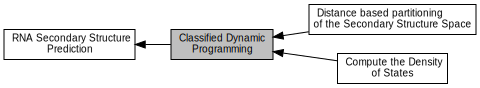
\includegraphics[width=350pt]{group__class__fold}
\end{center}
\end{figure}
\subsection*{Modules}
\begin{DoxyCompactItemize}
\item 
\hyperlink{group__kl__neighborhood}{Distance based partitioning of the Secondary Structure Space}
\begin{DoxyCompactList}\small\item\em Compute Thermodynamic properties for a Distance Class Partitioning of the Secondary Structure Space. \end{DoxyCompactList}\item 
\hyperlink{group__dos}{Compute the Density of States}
\end{DoxyCompactItemize}


\subsection{Detailed Description}

\include{group__kl__neighborhood}
\hypertarget{group__kl__neighborhood__mfe}{\section{Calculating M\+F\+E representatives of a Distance Based Partitioning}
\label{group__kl__neighborhood__mfe}\index{Calculating M\+F\+E representatives of a Distance Based Partitioning@{Calculating M\+F\+E representatives of a Distance Based Partitioning}}
}


Compute the minimum free energy (M\+F\+E) and secondary structures for a partitioning of the secondary structure space according to the base pair distance to two fixed reference structures basepair distance to two fixed reference structures.  


Collaboration diagram for Calculating M\+F\+E representatives of a Distance Based Partitioning\+:
\nopagebreak
\begin{figure}[H]
\begin{center}
\leavevmode
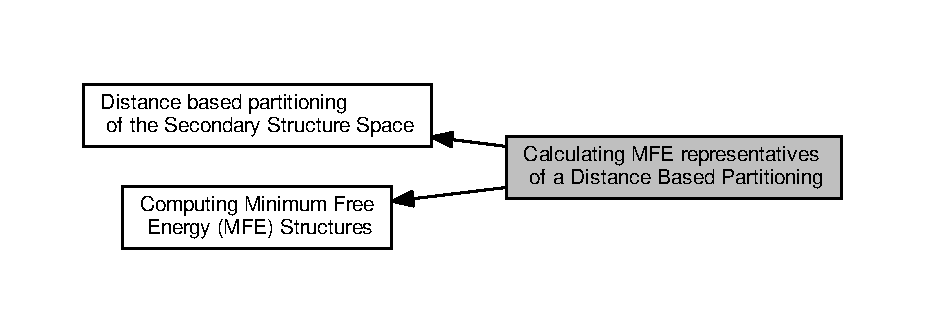
\includegraphics[width=350pt]{group__kl__neighborhood__mfe}
\end{center}
\end{figure}
\subsection*{Files}
\begin{DoxyCompactItemize}
\item 
file \hyperlink{2Dfold_8h}{2\+Dfold.\+h}
\end{DoxyCompactItemize}
\subsection*{Data Structures}
\begin{DoxyCompactItemize}
\item 
struct \hyperlink{group__kl__neighborhood__mfe_structvrna__sol__TwoD__t}{vrna\+\_\+sol\+\_\+\+Two\+D\+\_\+t}
\begin{DoxyCompactList}\small\item\em Solution element returned from \hyperlink{group__kl__neighborhood__mfe_ga243c288b463147352829df04de6a2f77}{vrna\+\_\+mfe\+\_\+\+Two\+D()}  \hyperlink{group__kl__neighborhood__mfe_structvrna__sol__TwoD__t}{More...}\end{DoxyCompactList}\item 
struct \hyperlink{group__kl__neighborhood__mfe_structTwoDfold__vars}{Two\+Dfold\+\_\+vars}
\begin{DoxyCompactList}\small\item\em Variables compound for 2\+Dfold M\+F\+E folding.  \hyperlink{group__kl__neighborhood__mfe_structTwoDfold__vars}{More...}\end{DoxyCompactList}\end{DoxyCompactItemize}
\subsection*{Typedefs}
\begin{DoxyCompactItemize}
\item 
typedef struct \hyperlink{group__kl__neighborhood__mfe_structvrna__sol__TwoD__t}{vrna\+\_\+sol\+\_\+\+Two\+D\+\_\+t} \hyperlink{group__kl__neighborhood__mfe_ga6a81a58268d250309712549a3fa0aab2}{vrna\+\_\+sol\+\_\+\+Two\+D\+\_\+t}
\begin{DoxyCompactList}\small\item\em Solution element returned from \hyperlink{group__kl__neighborhood__mfe_ga243c288b463147352829df04de6a2f77}{vrna\+\_\+mfe\+\_\+\+Two\+D()} \end{DoxyCompactList}\item 
typedef struct \hyperlink{group__kl__neighborhood__mfe_structTwoDfold__vars}{Two\+Dfold\+\_\+vars} \hyperlink{group__kl__neighborhood__mfe_gaf4f514010a14f9d59d850742b3e96954}{Two\+Dfold\+\_\+vars}
\begin{DoxyCompactList}\small\item\em Variables compound for 2\+Dfold M\+F\+E folding. \end{DoxyCompactList}\end{DoxyCompactItemize}
\subsection*{Functions}
\begin{DoxyCompactItemize}
\item 
\hyperlink{group__kl__neighborhood__mfe_structvrna__sol__TwoD__t}{vrna\+\_\+sol\+\_\+\+Two\+D\+\_\+t} $\ast$ \hyperlink{group__kl__neighborhood__mfe_ga243c288b463147352829df04de6a2f77}{vrna\+\_\+mfe\+\_\+\+Two\+D} (\hyperlink{group__fold__compound_ga1b0cef17fd40466cef5968eaeeff6166}{vrna\+\_\+fold\+\_\+compound\+\_\+t} $\ast$vc, int distance1, int distance2)
\begin{DoxyCompactList}\small\item\em Compute M\+F\+E's and representative for distance partitioning. \end{DoxyCompactList}\item 
char $\ast$ \hyperlink{group__kl__neighborhood__mfe_ga15a96fc96f4f4c2e01a11b3e17d1ef43}{vrna\+\_\+backtrack5\+\_\+\+Two\+D} (\hyperlink{group__fold__compound_ga1b0cef17fd40466cef5968eaeeff6166}{vrna\+\_\+fold\+\_\+compound\+\_\+t} $\ast$vc, int k, int l, unsigned int j)
\begin{DoxyCompactList}\small\item\em Backtrack a minimum free energy structure from a 5' section of specified length. \end{DoxyCompactList}\item 
\hyperlink{group__kl__neighborhood__mfe_structTwoDfold__vars}{Two\+Dfold\+\_\+vars} $\ast$ \hyperlink{group__kl__neighborhood__mfe_gac9284f132cf0eaa0a2f43590eda05488}{get\+\_\+\+Two\+Dfold\+\_\+variables} (const char $\ast$seq, const char $\ast$structure1, const char $\ast$structure2, int \hyperlink{group__model__details_gaf9202a1a09f5828dc731e2d9a10fa111}{circ})
\begin{DoxyCompactList}\small\item\em Get a structure of type \hyperlink{group__kl__neighborhood__mfe_structTwoDfold__vars}{Two\+Dfold\+\_\+vars} prefilled with current global settings. \end{DoxyCompactList}\item 
void \hyperlink{group__kl__neighborhood__mfe_ga05bf4f31d216b1b160fd2d3d68e9b487}{destroy\+\_\+\+Two\+Dfold\+\_\+variables} (\hyperlink{group__kl__neighborhood__mfe_structTwoDfold__vars}{Two\+Dfold\+\_\+vars} $\ast$our\+\_\+variables)
\begin{DoxyCompactList}\small\item\em Destroy a \hyperlink{group__kl__neighborhood__mfe_structTwoDfold__vars}{Two\+Dfold\+\_\+vars} datastructure without memory loss. \end{DoxyCompactList}\item 
\hyperlink{group__kl__neighborhood__mfe_structvrna__sol__TwoD__t}{vrna\+\_\+sol\+\_\+\+Two\+D\+\_\+t} $\ast$ \hyperlink{group__kl__neighborhood__mfe_ga7fc5e3e92fe97914ca4eccd33c01c2a7}{Two\+Dfold\+List} (\hyperlink{group__kl__neighborhood__mfe_structTwoDfold__vars}{Two\+Dfold\+\_\+vars} $\ast$vars, int distance1, int distance2)
\begin{DoxyCompactList}\small\item\em Compute M\+F\+E's and representative for distance partitioning. \end{DoxyCompactList}\item 
char $\ast$ \hyperlink{group__kl__neighborhood__mfe_gaf4dc05bf8fc1ea53acd7aeb798ba80c2}{Two\+Dfold\+\_\+backtrack\+\_\+f5} (unsigned int j, int k, int l, \hyperlink{group__kl__neighborhood__mfe_structTwoDfold__vars}{Two\+Dfold\+\_\+vars} $\ast$vars)
\begin{DoxyCompactList}\small\item\em Backtrack a minimum free energy structure from a 5' section of specified length. \end{DoxyCompactList}\end{DoxyCompactItemize}


\subsection{Detailed Description}
Compute the minimum free energy (M\+F\+E) and secondary structures for a partitioning of the secondary structure space according to the base pair distance to two fixed reference structures basepair distance to two fixed reference structures. 

\begin{DoxySeeAlso}{See also}
For further details, we refer to Lorenz et al. 2009 \cite{lorenz:2009} 
\end{DoxySeeAlso}


\subsection{Data Structure Documentation}
\index{vrna\+\_\+sol\+\_\+\+Two\+D\+\_\+t@{vrna\+\_\+sol\+\_\+\+Two\+D\+\_\+t}}\label{structvrna__sol__TwoD__t}
\hypertarget{group__kl__neighborhood__mfe_structvrna__sol__TwoD__t}{}
\subsubsection{struct vrna\+\_\+sol\+\_\+\+Two\+D\+\_\+t}
Solution element returned from \hyperlink{group__kl__neighborhood__mfe_ga243c288b463147352829df04de6a2f77}{vrna\+\_\+mfe\+\_\+\+Two\+D()} 

This element contains free energy and structure for the appropriate kappa (k), lambda (l) neighborhood The datastructure contains two integer attributes 'k' and 'l' as well as an attribute 'en' of type float representing the free energy in kcal/mol and an attribute 's' of type char$\ast$ containg the secondary structure representative,

A value of \hyperlink{energy__const_8h_a12c2040f25d8e3a7b9e1c2024c618cb6}{I\+N\+F} in k denotes the end of a list

\begin{DoxySeeAlso}{See also}
\hyperlink{group__kl__neighborhood__mfe_ga243c288b463147352829df04de6a2f77}{vrna\+\_\+mfe\+\_\+\+Two\+D()} 
\end{DoxySeeAlso}
\subsubsection*{Data Fields}
\begin{DoxyCompactItemize}
\item 
\hypertarget{group__kl__neighborhood__mfe_ac111e850bb3b3a11b6b5707912cfa1b8}{int \hyperlink{group__kl__neighborhood__mfe_ac111e850bb3b3a11b6b5707912cfa1b8}{k}}\label{group__kl__neighborhood__mfe_ac111e850bb3b3a11b6b5707912cfa1b8}

\begin{DoxyCompactList}\small\item\em Distance to first reference. \end{DoxyCompactList}\item 
\hypertarget{group__kl__neighborhood__mfe_ab8e95cd920901175a2cc8de726ab1d36}{int \hyperlink{group__kl__neighborhood__mfe_ab8e95cd920901175a2cc8de726ab1d36}{l}}\label{group__kl__neighborhood__mfe_ab8e95cd920901175a2cc8de726ab1d36}

\begin{DoxyCompactList}\small\item\em Distance to second reference. \end{DoxyCompactList}\item 
\hypertarget{group__kl__neighborhood__mfe_a7577863a6a84224dfee39b321c03cab1}{float \hyperlink{group__kl__neighborhood__mfe_a7577863a6a84224dfee39b321c03cab1}{en}}\label{group__kl__neighborhood__mfe_a7577863a6a84224dfee39b321c03cab1}

\begin{DoxyCompactList}\small\item\em Free energy in kcal/mol. \end{DoxyCompactList}\item 
\hypertarget{group__kl__neighborhood__mfe_ac5942d2505a6cd7e4a8073a321d5d2d5}{char $\ast$ \hyperlink{group__kl__neighborhood__mfe_ac5942d2505a6cd7e4a8073a321d5d2d5}{s}}\label{group__kl__neighborhood__mfe_ac5942d2505a6cd7e4a8073a321d5d2d5}

\begin{DoxyCompactList}\small\item\em M\+F\+E representative structure in dot-\/bracket notation. \end{DoxyCompactList}\end{DoxyCompactItemize}
\index{Two\+Dfold\+\_\+vars@{Two\+Dfold\+\_\+vars}}\label{structTwoDfold__vars}
\hypertarget{group__kl__neighborhood__mfe_structTwoDfold__vars}{}
\subsubsection{struct Two\+Dfold\+\_\+vars}
Variables compound for 2\+Dfold M\+F\+E folding. 

\begin{DoxyRefDesc}{Deprecated}
\item[\hyperlink{deprecated__deprecated000001}{Deprecated}]This data structure will be removed from the library soon! Use \hyperlink{group__fold__compound_ga1b0cef17fd40466cef5968eaeeff6166}{vrna\+\_\+fold\+\_\+compound\+\_\+t} and the corresponding functions vrna\+\_\+fold\+\_\+compound\+\_\+\+Two\+D(), \hyperlink{group__kl__neighborhood__mfe_ga243c288b463147352829df04de6a2f77}{vrna\+\_\+mfe\+\_\+\+Two\+D()}, and \hyperlink{group__fold__compound_gadded6039d63f5d6509836e20321534ad}{vrna\+\_\+fold\+\_\+compound\+\_\+free()} instead! \end{DoxyRefDesc}


Collaboration diagram for Two\+Dfold\+\_\+vars\+:
\nopagebreak
\begin{figure}[H]
\begin{center}
\leavevmode
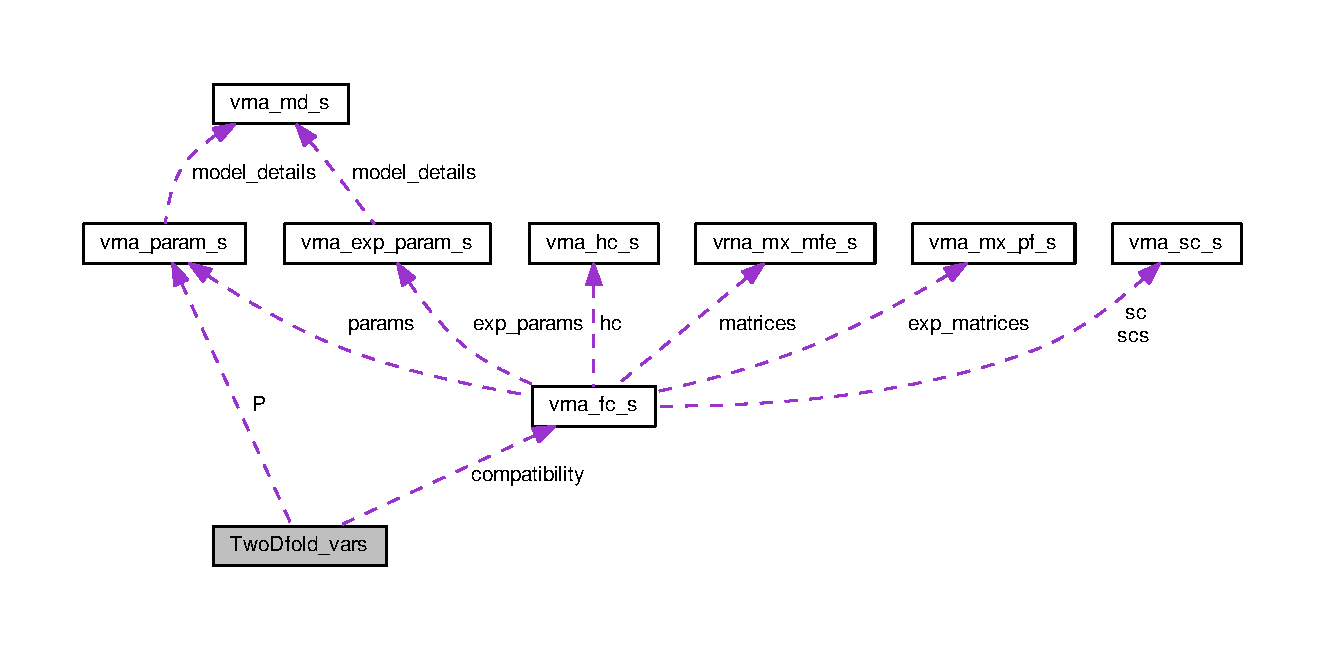
\includegraphics[width=350pt]{structTwoDfold__vars__coll__graph}
\end{center}
\end{figure}
\subsubsection*{Data Fields}
\begin{DoxyCompactItemize}
\item 
\hypertarget{group__kl__neighborhood__mfe_a70da9e83ad87c37013b4bf0b265dd307}{\hyperlink{group__energy__parameters_ga8a69ca7d787e4fd6079914f5343a1f35}{vrna\+\_\+param\+\_\+t} $\ast$ \hyperlink{group__kl__neighborhood__mfe_a70da9e83ad87c37013b4bf0b265dd307}{P}}\label{group__kl__neighborhood__mfe_a70da9e83ad87c37013b4bf0b265dd307}

\begin{DoxyCompactList}\small\item\em Precomputed energy parameters and model details. \end{DoxyCompactList}\item 
\hypertarget{group__kl__neighborhood__mfe_ade5c7e9337a458ae20bac75abdc52d64}{int \hyperlink{group__kl__neighborhood__mfe_ade5c7e9337a458ae20bac75abdc52d64}{do\+\_\+backtrack}}\label{group__kl__neighborhood__mfe_ade5c7e9337a458ae20bac75abdc52d64}

\begin{DoxyCompactList}\small\item\em Flag whether to do backtracing of the structure(s) or not. \end{DoxyCompactList}\item 
\hypertarget{group__kl__neighborhood__mfe_aedf60b8b26dae05ad266d3e098d18208}{char $\ast$ \hyperlink{group__kl__neighborhood__mfe_aedf60b8b26dae05ad266d3e098d18208}{ptype}}\label{group__kl__neighborhood__mfe_aedf60b8b26dae05ad266d3e098d18208}

\begin{DoxyCompactList}\small\item\em Precomputed array of pair types. \end{DoxyCompactList}\item 
\hypertarget{group__kl__neighborhood__mfe_a3596f3d4d320318c4b8428e2abc7ab56}{char $\ast$ \hyperlink{group__kl__neighborhood__mfe_a3596f3d4d320318c4b8428e2abc7ab56}{sequence}}\label{group__kl__neighborhood__mfe_a3596f3d4d320318c4b8428e2abc7ab56}

\begin{DoxyCompactList}\small\item\em The input sequence. \end{DoxyCompactList}\item 
\hypertarget{group__kl__neighborhood__mfe_ab9ee459ffbfb5d2c138a033516056cdc}{short $\ast$ \hyperlink{group__kl__neighborhood__mfe_ab9ee459ffbfb5d2c138a033516056cdc}{S1}}\label{group__kl__neighborhood__mfe_ab9ee459ffbfb5d2c138a033516056cdc}

\begin{DoxyCompactList}\small\item\em The input sequences in numeric form. \end{DoxyCompactList}\item 
\hypertarget{group__kl__neighborhood__mfe_a621ed2ab02116f3f8f5e7120dec429eb}{unsigned int \hyperlink{group__kl__neighborhood__mfe_a621ed2ab02116f3f8f5e7120dec429eb}{max\+D1}}\label{group__kl__neighborhood__mfe_a621ed2ab02116f3f8f5e7120dec429eb}

\begin{DoxyCompactList}\small\item\em Maximum allowed base pair distance to first reference. \end{DoxyCompactList}\item 
\hypertarget{group__kl__neighborhood__mfe_a03f198a4abdb3b784486d2ba5c533aa4}{unsigned int \hyperlink{group__kl__neighborhood__mfe_a03f198a4abdb3b784486d2ba5c533aa4}{max\+D2}}\label{group__kl__neighborhood__mfe_a03f198a4abdb3b784486d2ba5c533aa4}

\begin{DoxyCompactList}\small\item\em Maximum allowed base pair distance to second reference. \end{DoxyCompactList}\item 
\hypertarget{group__kl__neighborhood__mfe_aa11f5bcd8c4fe70a91c155c877c855d5}{unsigned int $\ast$ \hyperlink{group__kl__neighborhood__mfe_aa11f5bcd8c4fe70a91c155c877c855d5}{mm1}}\label{group__kl__neighborhood__mfe_aa11f5bcd8c4fe70a91c155c877c855d5}

\begin{DoxyCompactList}\small\item\em Maximum matching matrix, reference struct 1 disallowed. \end{DoxyCompactList}\item 
\hypertarget{group__kl__neighborhood__mfe_a2eaa93316b6beb17531f0c078806036c}{unsigned int $\ast$ \hyperlink{group__kl__neighborhood__mfe_a2eaa93316b6beb17531f0c078806036c}{mm2}}\label{group__kl__neighborhood__mfe_a2eaa93316b6beb17531f0c078806036c}

\begin{DoxyCompactList}\small\item\em Maximum matching matrix, reference struct 2 disallowed. \end{DoxyCompactList}\item 
\hypertarget{group__kl__neighborhood__mfe_a1a20cb06b58b75d1a3dbdbc8bc60d0a7}{int $\ast$ \hyperlink{group__kl__neighborhood__mfe_a1a20cb06b58b75d1a3dbdbc8bc60d0a7}{my\+\_\+iindx}}\label{group__kl__neighborhood__mfe_a1a20cb06b58b75d1a3dbdbc8bc60d0a7}

\begin{DoxyCompactList}\small\item\em Index for moving in quadratic distancy dimensions. \end{DoxyCompactList}\item 
\hypertarget{group__kl__neighborhood__mfe_a536525b98c1b633d4c5f2da4f8d78c18}{unsigned int $\ast$ \hyperlink{group__kl__neighborhood__mfe_a536525b98c1b633d4c5f2da4f8d78c18}{reference\+B\+Ps1}}\label{group__kl__neighborhood__mfe_a536525b98c1b633d4c5f2da4f8d78c18}

\begin{DoxyCompactList}\small\item\em Matrix containing number of basepairs of reference structure1 in interval \mbox{[}i,j\mbox{]}. \end{DoxyCompactList}\item 
\hypertarget{group__kl__neighborhood__mfe_aa7abf73c3114cb5f0dc90e702fa9dd0f}{unsigned int $\ast$ \hyperlink{group__kl__neighborhood__mfe_aa7abf73c3114cb5f0dc90e702fa9dd0f}{reference\+B\+Ps2}}\label{group__kl__neighborhood__mfe_aa7abf73c3114cb5f0dc90e702fa9dd0f}

\begin{DoxyCompactList}\small\item\em Matrix containing number of basepairs of reference structure2 in interval \mbox{[}i,j\mbox{]}. \end{DoxyCompactList}\item 
\hypertarget{group__kl__neighborhood__mfe_af1106e1a592e2dccc92b3452340549e0}{unsigned int $\ast$ \hyperlink{group__kl__neighborhood__mfe_af1106e1a592e2dccc92b3452340549e0}{bpdist}}\label{group__kl__neighborhood__mfe_af1106e1a592e2dccc92b3452340549e0}

\begin{DoxyCompactList}\small\item\em Matrix containing base pair distance of reference structure 1 and 2 on interval \mbox{[}i,j\mbox{]}. \end{DoxyCompactList}\end{DoxyCompactItemize}


\subsection{Typedef Documentation}
\hypertarget{group__kl__neighborhood__mfe_ga6a81a58268d250309712549a3fa0aab2}{\index{Calculating M\+F\+E representatives of a Distance Based Partitioning@{Calculating M\+F\+E representatives of a Distance Based Partitioning}!vrna\+\_\+sol\+\_\+\+Two\+D\+\_\+t@{vrna\+\_\+sol\+\_\+\+Two\+D\+\_\+t}}
\index{vrna\+\_\+sol\+\_\+\+Two\+D\+\_\+t@{vrna\+\_\+sol\+\_\+\+Two\+D\+\_\+t}!Calculating M\+F\+E representatives of a Distance Based Partitioning@{Calculating M\+F\+E representatives of a Distance Based Partitioning}}
\subsubsection[{vrna\+\_\+sol\+\_\+\+Two\+D\+\_\+t}]{\setlength{\rightskip}{0pt plus 5cm}typedef struct {\bf vrna\+\_\+sol\+\_\+\+Two\+D\+\_\+t}  {\bf vrna\+\_\+sol\+\_\+\+Two\+D\+\_\+t}}}\label{group__kl__neighborhood__mfe_ga6a81a58268d250309712549a3fa0aab2}


{\ttfamily \#include $<$\hyperlink{2Dfold_8h}{Vienna\+R\+N\+A/2\+Dfold.\+h}$>$}



Solution element returned from \hyperlink{group__kl__neighborhood__mfe_ga243c288b463147352829df04de6a2f77}{vrna\+\_\+mfe\+\_\+\+Two\+D()} 

This element contains free energy and structure for the appropriate kappa (k), lambda (l) neighborhood The datastructure contains two integer attributes 'k' and 'l' as well as an attribute 'en' of type float representing the free energy in kcal/mol and an attribute 's' of type char$\ast$ containg the secondary structure representative,

A value of \hyperlink{energy__const_8h_a12c2040f25d8e3a7b9e1c2024c618cb6}{I\+N\+F} in k denotes the end of a list

\begin{DoxySeeAlso}{See also}
\hyperlink{group__kl__neighborhood__mfe_ga243c288b463147352829df04de6a2f77}{vrna\+\_\+mfe\+\_\+\+Two\+D()} 
\end{DoxySeeAlso}
\hypertarget{group__kl__neighborhood__mfe_gaf4f514010a14f9d59d850742b3e96954}{\index{Calculating M\+F\+E representatives of a Distance Based Partitioning@{Calculating M\+F\+E representatives of a Distance Based Partitioning}!Two\+Dfold\+\_\+vars@{Two\+Dfold\+\_\+vars}}
\index{Two\+Dfold\+\_\+vars@{Two\+Dfold\+\_\+vars}!Calculating M\+F\+E representatives of a Distance Based Partitioning@{Calculating M\+F\+E representatives of a Distance Based Partitioning}}
\subsubsection[{Two\+Dfold\+\_\+vars}]{\setlength{\rightskip}{0pt plus 5cm}typedef struct {\bf Two\+Dfold\+\_\+vars}  {\bf Two\+Dfold\+\_\+vars}}}\label{group__kl__neighborhood__mfe_gaf4f514010a14f9d59d850742b3e96954}


{\ttfamily \#include $<$\hyperlink{2Dfold_8h}{Vienna\+R\+N\+A/2\+Dfold.\+h}$>$}



Variables compound for 2\+Dfold M\+F\+E folding. 

\begin{DoxyRefDesc}{Deprecated}
\item[\hyperlink{deprecated__deprecated000001}{Deprecated}]This data structure will be removed from the library soon! Use \hyperlink{group__fold__compound_ga1b0cef17fd40466cef5968eaeeff6166}{vrna\+\_\+fold\+\_\+compound\+\_\+t} and the corresponding functions vrna\+\_\+fold\+\_\+compound\+\_\+\+Two\+D(), \hyperlink{group__kl__neighborhood__mfe_ga243c288b463147352829df04de6a2f77}{vrna\+\_\+mfe\+\_\+\+Two\+D()}, and \hyperlink{group__fold__compound_gadded6039d63f5d6509836e20321534ad}{vrna\+\_\+fold\+\_\+compound\+\_\+free()} instead! \end{DoxyRefDesc}


\subsection{Function Documentation}
\hypertarget{group__kl__neighborhood__mfe_ga243c288b463147352829df04de6a2f77}{\index{Calculating M\+F\+E representatives of a Distance Based Partitioning@{Calculating M\+F\+E representatives of a Distance Based Partitioning}!vrna\+\_\+mfe\+\_\+\+Two\+D@{vrna\+\_\+mfe\+\_\+\+Two\+D}}
\index{vrna\+\_\+mfe\+\_\+\+Two\+D@{vrna\+\_\+mfe\+\_\+\+Two\+D}!Calculating M\+F\+E representatives of a Distance Based Partitioning@{Calculating M\+F\+E representatives of a Distance Based Partitioning}}
\subsubsection[{vrna\+\_\+mfe\+\_\+\+Two\+D}]{\setlength{\rightskip}{0pt plus 5cm}{\bf vrna\+\_\+sol\+\_\+\+Two\+D\+\_\+t}$\ast$ vrna\+\_\+mfe\+\_\+\+Two\+D (
\begin{DoxyParamCaption}
\item[{{\bf vrna\+\_\+fold\+\_\+compound\+\_\+t} $\ast$}]{vc, }
\item[{int}]{distance1, }
\item[{int}]{distance2}
\end{DoxyParamCaption}
)}}\label{group__kl__neighborhood__mfe_ga243c288b463147352829df04de6a2f77}


{\ttfamily \#include $<$\hyperlink{2Dfold_8h}{Vienna\+R\+N\+A/2\+Dfold.\+h}$>$}



Compute M\+F\+E's and representative for distance partitioning. 

This function computes the minimum free energies and a representative secondary structure for each distance class according to the two references specified in the datastructure 'vars'. The maximum basepair distance to each of both references may be set by the arguments 'distance1' and 'distance2', respectively. If both distance arguments are set to '-\/1', no restriction is assumed and the calculation is performed for each distance class possible.

The returned list contains an entry for each distance class. If a maximum basepair distance to either of the references was passed, an entry with k=l=-\/1 will be appended in the list, denoting the class where all structures exceeding the maximum will be thrown into. The end of the list is denoted by an attribute value of \hyperlink{energy__const_8h_a12c2040f25d8e3a7b9e1c2024c618cb6}{I\+N\+F} in the k-\/attribute of the list entry.

\begin{DoxySeeAlso}{See also}
vrna\+\_\+fold\+\_\+compound\+\_\+\+Two\+D(), \hyperlink{group__fold__compound_gadded6039d63f5d6509836e20321534ad}{vrna\+\_\+fold\+\_\+compound\+\_\+free()}, \hyperlink{group__kl__neighborhood__pf_ga0bc3427689bd09da09b8b3094a27f836}{vrna\+\_\+pf\+\_\+\+Two\+D()} \hyperlink{group__kl__neighborhood__mfe_ga15a96fc96f4f4c2e01a11b3e17d1ef43}{vrna\+\_\+backtrack5\+\_\+\+Two\+D()}, \hyperlink{group__kl__neighborhood__mfe_structvrna__sol__TwoD__t}{vrna\+\_\+sol\+\_\+\+Two\+D\+\_\+t}, \hyperlink{group__fold__compound_ga1b0cef17fd40466cef5968eaeeff6166}{vrna\+\_\+fold\+\_\+compound\+\_\+t}
\end{DoxySeeAlso}

\begin{DoxyParams}{Parameters}
{\em vc} & The datastructure containing all precomputed folding attributes \\
\hline
{\em distance1} & maximum distance to reference1 (-\/1 means no restriction) \\
\hline
{\em distance2} & maximum distance to reference2 (-\/1 means no restriction) \\
\hline
\end{DoxyParams}
\begin{DoxyReturn}{Returns}
A list of minimum free energies (and corresponding structures) for each distance class 
\end{DoxyReturn}
\hypertarget{group__kl__neighborhood__mfe_ga15a96fc96f4f4c2e01a11b3e17d1ef43}{\index{Calculating M\+F\+E representatives of a Distance Based Partitioning@{Calculating M\+F\+E representatives of a Distance Based Partitioning}!vrna\+\_\+backtrack5\+\_\+\+Two\+D@{vrna\+\_\+backtrack5\+\_\+\+Two\+D}}
\index{vrna\+\_\+backtrack5\+\_\+\+Two\+D@{vrna\+\_\+backtrack5\+\_\+\+Two\+D}!Calculating M\+F\+E representatives of a Distance Based Partitioning@{Calculating M\+F\+E representatives of a Distance Based Partitioning}}
\subsubsection[{vrna\+\_\+backtrack5\+\_\+\+Two\+D}]{\setlength{\rightskip}{0pt plus 5cm}char$\ast$ vrna\+\_\+backtrack5\+\_\+\+Two\+D (
\begin{DoxyParamCaption}
\item[{{\bf vrna\+\_\+fold\+\_\+compound\+\_\+t} $\ast$}]{vc, }
\item[{int}]{k, }
\item[{int}]{l, }
\item[{unsigned int}]{j}
\end{DoxyParamCaption}
)}}\label{group__kl__neighborhood__mfe_ga15a96fc96f4f4c2e01a11b3e17d1ef43}


{\ttfamily \#include $<$\hyperlink{2Dfold_8h}{Vienna\+R\+N\+A/2\+Dfold.\+h}$>$}



Backtrack a minimum free energy structure from a 5' section of specified length. 

This function allows to backtrack a secondary structure beginning at the 5' end, a specified length and residing in a specific distance class. If the argument 'k' gets a value of -\/1, the structure that is backtracked is assumed to reside in the distance class where all structures exceeding the maximum basepair distance specified in \hyperlink{group__kl__neighborhood__mfe_ga243c288b463147352829df04de6a2f77}{vrna\+\_\+mfe\+\_\+\+Two\+D()} belong to. \begin{DoxyNote}{Note}
The argument 'vars' must contain precalculated energy values in the energy matrices, i.\+e. a call to \hyperlink{group__kl__neighborhood__mfe_ga243c288b463147352829df04de6a2f77}{vrna\+\_\+mfe\+\_\+\+Two\+D()} preceding this function is mandatory!
\end{DoxyNote}
\begin{DoxySeeAlso}{See also}
\hyperlink{group__kl__neighborhood__mfe_ga243c288b463147352829df04de6a2f77}{vrna\+\_\+mfe\+\_\+\+Two\+D()}
\end{DoxySeeAlso}

\begin{DoxyParams}{Parameters}
{\em vc} & The datastructure containing all precomputed folding attributes \\
\hline
{\em j} & The length in nucleotides beginning from the 5' end \\
\hline
{\em k} & distance to reference1 (may be -\/1) \\
\hline
{\em l} & distance to reference2 \\
\hline
\end{DoxyParams}
\hypertarget{group__kl__neighborhood__mfe_gac9284f132cf0eaa0a2f43590eda05488}{\index{Calculating M\+F\+E representatives of a Distance Based Partitioning@{Calculating M\+F\+E representatives of a Distance Based Partitioning}!get\+\_\+\+Two\+Dfold\+\_\+variables@{get\+\_\+\+Two\+Dfold\+\_\+variables}}
\index{get\+\_\+\+Two\+Dfold\+\_\+variables@{get\+\_\+\+Two\+Dfold\+\_\+variables}!Calculating M\+F\+E representatives of a Distance Based Partitioning@{Calculating M\+F\+E representatives of a Distance Based Partitioning}}
\subsubsection[{get\+\_\+\+Two\+Dfold\+\_\+variables}]{\setlength{\rightskip}{0pt plus 5cm}{\bf Two\+Dfold\+\_\+vars}$\ast$ get\+\_\+\+Two\+Dfold\+\_\+variables (
\begin{DoxyParamCaption}
\item[{const char $\ast$}]{seq, }
\item[{const char $\ast$}]{structure1, }
\item[{const char $\ast$}]{structure2, }
\item[{int}]{circ}
\end{DoxyParamCaption}
)}}\label{group__kl__neighborhood__mfe_gac9284f132cf0eaa0a2f43590eda05488}


{\ttfamily \#include $<$\hyperlink{2Dfold_8h}{Vienna\+R\+N\+A/2\+Dfold.\+h}$>$}



Get a structure of type \hyperlink{group__kl__neighborhood__mfe_structTwoDfold__vars}{Two\+Dfold\+\_\+vars} prefilled with current global settings. 

This function returns a datastructure of type \hyperlink{group__kl__neighborhood__mfe_structTwoDfold__vars}{Two\+Dfold\+\_\+vars}. The data fields inside the \hyperlink{group__kl__neighborhood__mfe_structTwoDfold__vars}{Two\+Dfold\+\_\+vars} are prefilled by global settings and all memory allocations necessary to start a computation are already done for the convenience of the user

\begin{DoxyNote}{Note}
Make sure that the reference structures are compatible with the sequence according to Watson-\/\+Crick-\/ and Wobble-\/base pairing
\end{DoxyNote}
\begin{DoxyRefDesc}{Deprecated}
\item[\hyperlink{deprecated__deprecated000002}{Deprecated}]Use the new A\+P\+I that relies on \hyperlink{group__fold__compound_ga1b0cef17fd40466cef5968eaeeff6166}{vrna\+\_\+fold\+\_\+compound\+\_\+t} and the corresponding functions vrna\+\_\+fold\+\_\+compound\+\_\+\+Two\+D(), \hyperlink{group__kl__neighborhood__mfe_ga243c288b463147352829df04de6a2f77}{vrna\+\_\+mfe\+\_\+\+Two\+D()}, and \hyperlink{group__fold__compound_gadded6039d63f5d6509836e20321534ad}{vrna\+\_\+fold\+\_\+compound\+\_\+free()} instead!\end{DoxyRefDesc}



\begin{DoxyParams}{Parameters}
{\em seq} & The R\+N\+A sequence \\
\hline
{\em structure1} & The first reference structure in dot-\/bracket notation \\
\hline
{\em structure2} & The second reference structure in dot-\/bracket notation \\
\hline
{\em circ} & A switch to indicate the assumption to fold a circular instead of linear R\+N\+A (0=O\+F\+F, 1=O\+N) \\
\hline
\end{DoxyParams}
\begin{DoxyReturn}{Returns}
A datastructure prefilled with folding options and allocated memory 
\end{DoxyReturn}
\hypertarget{group__kl__neighborhood__mfe_ga05bf4f31d216b1b160fd2d3d68e9b487}{\index{Calculating M\+F\+E representatives of a Distance Based Partitioning@{Calculating M\+F\+E representatives of a Distance Based Partitioning}!destroy\+\_\+\+Two\+Dfold\+\_\+variables@{destroy\+\_\+\+Two\+Dfold\+\_\+variables}}
\index{destroy\+\_\+\+Two\+Dfold\+\_\+variables@{destroy\+\_\+\+Two\+Dfold\+\_\+variables}!Calculating M\+F\+E representatives of a Distance Based Partitioning@{Calculating M\+F\+E representatives of a Distance Based Partitioning}}
\subsubsection[{destroy\+\_\+\+Two\+Dfold\+\_\+variables}]{\setlength{\rightskip}{0pt plus 5cm}void destroy\+\_\+\+Two\+Dfold\+\_\+variables (
\begin{DoxyParamCaption}
\item[{{\bf Two\+Dfold\+\_\+vars} $\ast$}]{our\+\_\+variables}
\end{DoxyParamCaption}
)}}\label{group__kl__neighborhood__mfe_ga05bf4f31d216b1b160fd2d3d68e9b487}


{\ttfamily \#include $<$\hyperlink{2Dfold_8h}{Vienna\+R\+N\+A/2\+Dfold.\+h}$>$}



Destroy a \hyperlink{group__kl__neighborhood__mfe_structTwoDfold__vars}{Two\+Dfold\+\_\+vars} datastructure without memory loss. 

This function free's all allocated memory that depends on the datastructure given.

\begin{DoxyRefDesc}{Deprecated}
\item[\hyperlink{deprecated__deprecated000003}{Deprecated}]Use the new A\+P\+I that relies on \hyperlink{group__fold__compound_ga1b0cef17fd40466cef5968eaeeff6166}{vrna\+\_\+fold\+\_\+compound\+\_\+t} and the corresponding functions vrna\+\_\+fold\+\_\+compound\+\_\+\+Two\+D(), \hyperlink{group__kl__neighborhood__mfe_ga243c288b463147352829df04de6a2f77}{vrna\+\_\+mfe\+\_\+\+Two\+D()}, and \hyperlink{group__fold__compound_gadded6039d63f5d6509836e20321534ad}{vrna\+\_\+fold\+\_\+compound\+\_\+free()} instead!\end{DoxyRefDesc}



\begin{DoxyParams}{Parameters}
{\em our\+\_\+variables} & A pointer to the datastructure to be destroyed \\
\hline
\end{DoxyParams}
\hypertarget{group__kl__neighborhood__mfe_ga7fc5e3e92fe97914ca4eccd33c01c2a7}{\index{Calculating M\+F\+E representatives of a Distance Based Partitioning@{Calculating M\+F\+E representatives of a Distance Based Partitioning}!Two\+Dfold\+List@{Two\+Dfold\+List}}
\index{Two\+Dfold\+List@{Two\+Dfold\+List}!Calculating M\+F\+E representatives of a Distance Based Partitioning@{Calculating M\+F\+E representatives of a Distance Based Partitioning}}
\subsubsection[{Two\+Dfold\+List}]{\setlength{\rightskip}{0pt plus 5cm}{\bf vrna\+\_\+sol\+\_\+\+Two\+D\+\_\+t}$\ast$ Two\+Dfold\+List (
\begin{DoxyParamCaption}
\item[{{\bf Two\+Dfold\+\_\+vars} $\ast$}]{vars, }
\item[{int}]{distance1, }
\item[{int}]{distance2}
\end{DoxyParamCaption}
)}}\label{group__kl__neighborhood__mfe_ga7fc5e3e92fe97914ca4eccd33c01c2a7}


{\ttfamily \#include $<$\hyperlink{2Dfold_8h}{Vienna\+R\+N\+A/2\+Dfold.\+h}$>$}



Compute M\+F\+E's and representative for distance partitioning. 

This function computes the minimum free energies and a representative secondary structure for each distance class according to the two references specified in the datastructure 'vars'. The maximum basepair distance to each of both references may be set by the arguments 'distance1' and 'distance2', respectively. If both distance arguments are set to '-\/1', no restriction is assumed and the calculation is performed for each distance class possible.

The returned list contains an entry for each distance class. If a maximum basepair distance to either of the references was passed, an entry with k=l=-\/1 will be appended in the list, denoting the class where all structures exceeding the maximum will be thrown into. The end of the list is denoted by an attribute value of \hyperlink{energy__const_8h_a12c2040f25d8e3a7b9e1c2024c618cb6}{I\+N\+F} in the k-\/attribute of the list entry.

\begin{DoxyRefDesc}{Deprecated}
\item[\hyperlink{deprecated__deprecated000004}{Deprecated}]Use the new A\+P\+I that relies on \hyperlink{group__fold__compound_ga1b0cef17fd40466cef5968eaeeff6166}{vrna\+\_\+fold\+\_\+compound\+\_\+t} and the corresponding functions vrna\+\_\+fold\+\_\+compound\+\_\+\+Two\+D(), \hyperlink{group__kl__neighborhood__mfe_ga243c288b463147352829df04de6a2f77}{vrna\+\_\+mfe\+\_\+\+Two\+D()}, and \hyperlink{group__fold__compound_gadded6039d63f5d6509836e20321534ad}{vrna\+\_\+fold\+\_\+compound\+\_\+free()} instead!\end{DoxyRefDesc}



\begin{DoxyParams}{Parameters}
{\em vars} & the datastructure containing all predefined folding attributes \\
\hline
{\em distance1} & maximum distance to reference1 (-\/1 means no restriction) \\
\hline
{\em distance2} & maximum distance to reference2 (-\/1 means no restriction) \\
\hline
\end{DoxyParams}
\hypertarget{group__kl__neighborhood__mfe_gaf4dc05bf8fc1ea53acd7aeb798ba80c2}{\index{Calculating M\+F\+E representatives of a Distance Based Partitioning@{Calculating M\+F\+E representatives of a Distance Based Partitioning}!Two\+Dfold\+\_\+backtrack\+\_\+f5@{Two\+Dfold\+\_\+backtrack\+\_\+f5}}
\index{Two\+Dfold\+\_\+backtrack\+\_\+f5@{Two\+Dfold\+\_\+backtrack\+\_\+f5}!Calculating M\+F\+E representatives of a Distance Based Partitioning@{Calculating M\+F\+E representatives of a Distance Based Partitioning}}
\subsubsection[{Two\+Dfold\+\_\+backtrack\+\_\+f5}]{\setlength{\rightskip}{0pt plus 5cm}char$\ast$ Two\+Dfold\+\_\+backtrack\+\_\+f5 (
\begin{DoxyParamCaption}
\item[{unsigned int}]{j, }
\item[{int}]{k, }
\item[{int}]{l, }
\item[{{\bf Two\+Dfold\+\_\+vars} $\ast$}]{vars}
\end{DoxyParamCaption}
)}}\label{group__kl__neighborhood__mfe_gaf4dc05bf8fc1ea53acd7aeb798ba80c2}


{\ttfamily \#include $<$\hyperlink{2Dfold_8h}{Vienna\+R\+N\+A/2\+Dfold.\+h}$>$}



Backtrack a minimum free energy structure from a 5' section of specified length. 

This function allows to backtrack a secondary structure beginning at the 5' end, a specified length and residing in a specific distance class. If the argument 'k' gets a value of -\/1, the structure that is backtracked is assumed to reside in the distance class where all structures exceeding the maximum basepair distance specified in Two\+Dfold() belong to. \begin{DoxyNote}{Note}
The argument 'vars' must contain precalculated energy values in the energy matrices, i.\+e. a call to Two\+Dfold() preceding this function is mandatory!
\end{DoxyNote}
\begin{DoxyRefDesc}{Deprecated}
\item[\hyperlink{deprecated__deprecated000005}{Deprecated}]Use the new A\+P\+I that relies on \hyperlink{group__fold__compound_ga1b0cef17fd40466cef5968eaeeff6166}{vrna\+\_\+fold\+\_\+compound\+\_\+t} and the corresponding functions vrna\+\_\+fold\+\_\+compound\+\_\+\+Two\+D(), \hyperlink{group__kl__neighborhood__mfe_ga243c288b463147352829df04de6a2f77}{vrna\+\_\+mfe\+\_\+\+Two\+D()}, \hyperlink{group__kl__neighborhood__mfe_ga15a96fc96f4f4c2e01a11b3e17d1ef43}{vrna\+\_\+backtrack5\+\_\+\+Two\+D()}, and \hyperlink{group__fold__compound_gadded6039d63f5d6509836e20321534ad}{vrna\+\_\+fold\+\_\+compound\+\_\+free()} instead!\end{DoxyRefDesc}



\begin{DoxyParams}{Parameters}
{\em j} & The length in nucleotides beginning from the 5' end \\
\hline
{\em k} & distance to reference1 (may be -\/1) \\
\hline
{\em l} & distance to reference2 \\
\hline
{\em vars} & the datastructure containing all predefined folding attributes \\
\hline
\end{DoxyParams}

\hypertarget{group__kl__neighborhood__pf}{}\section{Calculate Partition Functions of a Distance Based Partitioning}
\label{group__kl__neighborhood__pf}\index{Calculate Partition Functions of a Distance Based Partitioning@{Calculate Partition Functions of a Distance Based Partitioning}}


Compute the partition function and stochastically sample secondary structures for a partitioning of the secondary structure space according to the base pair distance to two fixed reference structures.  


Collaboration diagram for Calculate Partition Functions of a Distance Based Partitioning\+:
\nopagebreak
\begin{figure}[H]
\begin{center}
\leavevmode
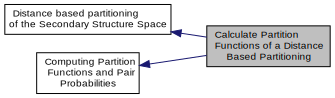
\includegraphics[width=350pt]{group__kl__neighborhood__pf}
\end{center}
\end{figure}
\subsection*{Files}
\begin{DoxyCompactItemize}
\item 
file \hyperlink{2Dpfold_8h}{2\+Dpfold.\+h}
\end{DoxyCompactItemize}
\subsection*{Data Structures}
\begin{DoxyCompactItemize}
\item 
struct \hyperlink{group__kl__neighborhood__pf_structvrna__sol__TwoD__pf__t}{vrna\+\_\+sol\+\_\+\+Two\+D\+\_\+pf\+\_\+t}
\begin{DoxyCompactList}\small\item\em Solution element returned from \hyperlink{group__kl__neighborhood__pf_ga0bc3427689bd09da09b8b3094a27f836}{vrna\+\_\+pf\+\_\+\+Two\+D()}  \hyperlink{group__kl__neighborhood__pf_structvrna__sol__TwoD__pf__t}{More...}\end{DoxyCompactList}\end{DoxyCompactItemize}
\subsection*{Typedefs}
\begin{DoxyCompactItemize}
\item 
typedef struct \hyperlink{group__kl__neighborhood__pf_structvrna__sol__TwoD__pf__t}{vrna\+\_\+sol\+\_\+\+Two\+D\+\_\+pf\+\_\+t} \hyperlink{group__kl__neighborhood__pf_ga5e449fbd695406aabd2bcabddc374621}{vrna\+\_\+sol\+\_\+\+Two\+D\+\_\+pf\+\_\+t}
\begin{DoxyCompactList}\small\item\em Solution element returned from \hyperlink{group__kl__neighborhood__pf_ga0bc3427689bd09da09b8b3094a27f836}{vrna\+\_\+pf\+\_\+\+Two\+D()} \end{DoxyCompactList}\end{DoxyCompactItemize}
\subsection*{Functions}
\begin{DoxyCompactItemize}
\item 
\hyperlink{group__kl__neighborhood__pf_structvrna__sol__TwoD__pf__t}{vrna\+\_\+sol\+\_\+\+Two\+D\+\_\+pf\+\_\+t} $\ast$ \hyperlink{group__kl__neighborhood__pf_ga0bc3427689bd09da09b8b3094a27f836}{vrna\+\_\+pf\+\_\+\+Two\+D} (\hyperlink{group__fold__compound_ga1b0cef17fd40466cef5968eaeeff6166}{vrna\+\_\+fold\+\_\+compound\+\_\+t} $\ast$vc, int max\+Distance1, int max\+Distance2)
\begin{DoxyCompactList}\small\item\em Compute the partition function for all distance classes. \end{DoxyCompactList}\end{DoxyCompactItemize}


\subsection{Detailed Description}
Compute the partition function and stochastically sample secondary structures for a partitioning of the secondary structure space according to the base pair distance to two fixed reference structures. 



\subsection{Data Structure Documentation}
\index{vrna\+\_\+sol\+\_\+\+Two\+D\+\_\+pf\+\_\+t@{vrna\+\_\+sol\+\_\+\+Two\+D\+\_\+pf\+\_\+t}}\label{structvrna__sol__TwoD__pf__t}
\hypertarget{group__kl__neighborhood__pf_structvrna__sol__TwoD__pf__t}{}
\subsubsection{struct vrna\+\_\+sol\+\_\+\+Two\+D\+\_\+pf\+\_\+t}
Solution element returned from \hyperlink{group__kl__neighborhood__pf_ga0bc3427689bd09da09b8b3094a27f836}{vrna\+\_\+pf\+\_\+\+Two\+D()} 

This element contains the partition function for the appropriate kappa (k), lambda (l) neighborhood The datastructure contains two integer attributes \textquotesingle{}k\textquotesingle{} and \textquotesingle{}l\textquotesingle{} as well as an attribute \textquotesingle{}q\textquotesingle{} of type \hyperlink{group__data__structures_ga31125aeace516926bf7f251f759b6126}{F\+L\+T\+\_\+\+O\+R\+\_\+\+D\+B\+L}

A value of \hyperlink{energy__const_8h_a12c2040f25d8e3a7b9e1c2024c618cb6}{I\+N\+F} in k denotes the end of a list

\begin{DoxySeeAlso}{See also}
\hyperlink{group__kl__neighborhood__pf_ga0bc3427689bd09da09b8b3094a27f836}{vrna\+\_\+pf\+\_\+\+Two\+D()} 
\end{DoxySeeAlso}
\subsubsection*{Data Fields}
\begin{DoxyCompactItemize}
\item 
\hypertarget{group__kl__neighborhood__pf_ad1f23b46dc4ebd373abdeb0382d87b83}{}int \hyperlink{group__kl__neighborhood__pf_ad1f23b46dc4ebd373abdeb0382d87b83}{k}\label{group__kl__neighborhood__pf_ad1f23b46dc4ebd373abdeb0382d87b83}

\begin{DoxyCompactList}\small\item\em Distance to first reference. \end{DoxyCompactList}\item 
\hypertarget{group__kl__neighborhood__pf_a01133c264eff2c988d144e07803d1b8b}{}int \hyperlink{group__kl__neighborhood__pf_a01133c264eff2c988d144e07803d1b8b}{l}\label{group__kl__neighborhood__pf_a01133c264eff2c988d144e07803d1b8b}

\begin{DoxyCompactList}\small\item\em Distance to second reference. \end{DoxyCompactList}\item 
\hypertarget{group__kl__neighborhood__pf_a17ebbf425b8769ded74b5c7b85e58ee1}{}\hyperlink{group__data__structures_ga31125aeace516926bf7f251f759b6126}{F\+L\+T\+\_\+\+O\+R\+\_\+\+D\+B\+L} \hyperlink{group__kl__neighborhood__pf_a17ebbf425b8769ded74b5c7b85e58ee1}{q}\label{group__kl__neighborhood__pf_a17ebbf425b8769ded74b5c7b85e58ee1}

\begin{DoxyCompactList}\small\item\em partition function \end{DoxyCompactList}\end{DoxyCompactItemize}


\subsection{Typedef Documentation}
\hypertarget{group__kl__neighborhood__pf_ga5e449fbd695406aabd2bcabddc374621}{}\index{Calculate Partition Functions of a Distance Based Partitioning@{Calculate Partition Functions of a Distance Based Partitioning}!vrna\+\_\+sol\+\_\+\+Two\+D\+\_\+pf\+\_\+t@{vrna\+\_\+sol\+\_\+\+Two\+D\+\_\+pf\+\_\+t}}
\index{vrna\+\_\+sol\+\_\+\+Two\+D\+\_\+pf\+\_\+t@{vrna\+\_\+sol\+\_\+\+Two\+D\+\_\+pf\+\_\+t}!Calculate Partition Functions of a Distance Based Partitioning@{Calculate Partition Functions of a Distance Based Partitioning}}
\subsubsection[{vrna\+\_\+sol\+\_\+\+Two\+D\+\_\+pf\+\_\+t}]{\setlength{\rightskip}{0pt plus 5cm}typedef struct {\bf vrna\+\_\+sol\+\_\+\+Two\+D\+\_\+pf\+\_\+t}  {\bf vrna\+\_\+sol\+\_\+\+Two\+D\+\_\+pf\+\_\+t}}\label{group__kl__neighborhood__pf_ga5e449fbd695406aabd2bcabddc374621}


{\ttfamily \#include $<$\hyperlink{2Dpfold_8h}{Vienna\+R\+N\+A/2\+Dpfold.\+h}$>$}



Solution element returned from \hyperlink{group__kl__neighborhood__pf_ga0bc3427689bd09da09b8b3094a27f836}{vrna\+\_\+pf\+\_\+\+Two\+D()} 

This element contains the partition function for the appropriate kappa (k), lambda (l) neighborhood The datastructure contains two integer attributes \textquotesingle{}k\textquotesingle{} and \textquotesingle{}l\textquotesingle{} as well as an attribute \textquotesingle{}q\textquotesingle{} of type \hyperlink{group__data__structures_ga31125aeace516926bf7f251f759b6126}{F\+L\+T\+\_\+\+O\+R\+\_\+\+D\+B\+L}

A value of \hyperlink{energy__const_8h_a12c2040f25d8e3a7b9e1c2024c618cb6}{I\+N\+F} in k denotes the end of a list

\begin{DoxySeeAlso}{See also}
\hyperlink{group__kl__neighborhood__pf_ga0bc3427689bd09da09b8b3094a27f836}{vrna\+\_\+pf\+\_\+\+Two\+D()} 
\end{DoxySeeAlso}


\subsection{Function Documentation}
\hypertarget{group__kl__neighborhood__pf_ga0bc3427689bd09da09b8b3094a27f836}{}\index{Calculate Partition Functions of a Distance Based Partitioning@{Calculate Partition Functions of a Distance Based Partitioning}!vrna\+\_\+pf\+\_\+\+Two\+D@{vrna\+\_\+pf\+\_\+\+Two\+D}}
\index{vrna\+\_\+pf\+\_\+\+Two\+D@{vrna\+\_\+pf\+\_\+\+Two\+D}!Calculate Partition Functions of a Distance Based Partitioning@{Calculate Partition Functions of a Distance Based Partitioning}}
\subsubsection[{vrna\+\_\+pf\+\_\+\+Two\+D}]{\setlength{\rightskip}{0pt plus 5cm}{\bf vrna\+\_\+sol\+\_\+\+Two\+D\+\_\+pf\+\_\+t}$\ast$ vrna\+\_\+pf\+\_\+\+Two\+D (
\begin{DoxyParamCaption}
\item[{{\bf vrna\+\_\+fold\+\_\+compound\+\_\+t} $\ast$}]{vc, }
\item[{int}]{max\+Distance1, }
\item[{int}]{max\+Distance2}
\end{DoxyParamCaption}
)}\label{group__kl__neighborhood__pf_ga0bc3427689bd09da09b8b3094a27f836}


{\ttfamily \#include $<$\hyperlink{2Dpfold_8h}{Vienna\+R\+N\+A/2\+Dpfold.\+h}$>$}



Compute the partition function for all distance classes. 

This function computes the partition functions for all distance classes according the two reference structures specified in the datastructure \textquotesingle{}vars\textquotesingle{}. Similar to \hyperlink{group__kl__neighborhood__mfe_ga243c288b463147352829df04de6a2f77}{vrna\+\_\+mfe\+\_\+\+Two\+D()} the arguments max\+Distance1 and max\+Distance2 specify the maximum distance to both reference structures. A value of \textquotesingle{}-\/1\textquotesingle{} in either of them makes the appropriate distance restrictionless, i.\+e. all basepair distancies to the reference are taken into account during computation. In case there is a restriction, the returned solution contains an entry where the attribute k=l=-\/1 contains the partition function for all structures exceeding the restriction. A value of \hyperlink{energy__const_8h_a12c2040f25d8e3a7b9e1c2024c618cb6}{I\+N\+F} in the attribute \textquotesingle{}k\textquotesingle{} of the returned list denotes the end of the list

\begin{DoxySeeAlso}{See also}
vrna\+\_\+fold\+\_\+compound\+\_\+\+Two\+D(), \hyperlink{group__fold__compound_gadded6039d63f5d6509836e20321534ad}{vrna\+\_\+fold\+\_\+compound\+\_\+free()}, \hyperlink{group__fold__compound_ga6601d994ba32b11511b36f68b08403be}{vrna\+\_\+fold\+\_\+compound} \hyperlink{group__kl__neighborhood__pf_structvrna__sol__TwoD__pf__t}{vrna\+\_\+sol\+\_\+\+Two\+D\+\_\+pf\+\_\+t}
\end{DoxySeeAlso}

\begin{DoxyParams}{Parameters}
{\em vc} & The datastructure containing all necessary folding attributes and matrices \\
\hline
{\em max\+Distance1} & The maximum basepair distance to reference1 (may be -\/1) \\
\hline
{\em max\+Distance2} & The maximum basepair distance to reference2 (may be -\/1) \\
\hline
\end{DoxyParams}
\begin{DoxyReturn}{Returns}
A list of partition funtions for the corresponding distance classes 
\end{DoxyReturn}

\hypertarget{group__kl__neighborhood__stochbt}{}\section{Stochastic Backtracking of Structures from Distance Based Partitioning}
\label{group__kl__neighborhood__stochbt}\index{Stochastic Backtracking of Structures from Distance Based Partitioning@{Stochastic Backtracking of Structures from Distance Based Partitioning}}


Contains functions related to stochastic backtracking from a specified distance class.  


Collaboration diagram for Stochastic Backtracking of Structures from Distance Based Partitioning\+:
\nopagebreak
\begin{figure}[H]
\begin{center}
\leavevmode
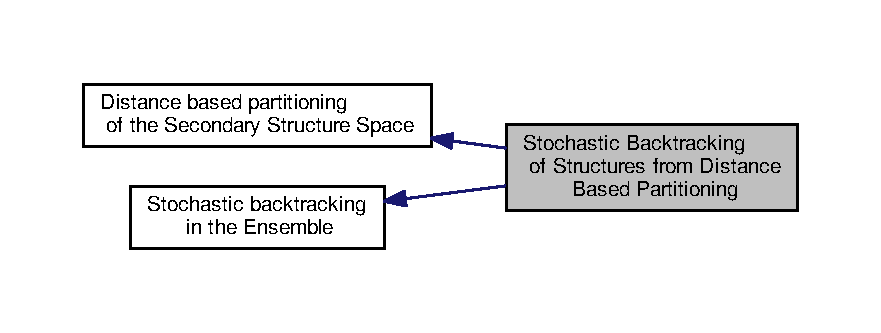
\includegraphics[width=350pt]{group__kl__neighborhood__stochbt}
\end{center}
\end{figure}
\subsection*{Functions}
\begin{DoxyCompactItemize}
\item 
char $\ast$ \hyperlink{group__kl__neighborhood__stochbt_ga14aceef73f83bbde77bb3a0ca06c9d13}{vrna\+\_\+pbacktrack\+\_\+\+Two\+D} (\hyperlink{group__fold__compound_ga1b0cef17fd40466cef5968eaeeff6166}{vrna\+\_\+fold\+\_\+compound\+\_\+t} $\ast$vc, int d1, int d2)
\begin{DoxyCompactList}\small\item\em Sample secondary structure representatives from a set of distance classes according to their Boltzmann probability. \end{DoxyCompactList}\item 
char $\ast$ \hyperlink{group__kl__neighborhood__stochbt_ga6504913303bc325659c365d5f59b41e0}{vrna\+\_\+pbacktrack5\+\_\+\+Two\+D} (\hyperlink{group__fold__compound_ga1b0cef17fd40466cef5968eaeeff6166}{vrna\+\_\+fold\+\_\+compound\+\_\+t} $\ast$vc, int d1, int d2, unsigned int length)
\begin{DoxyCompactList}\small\item\em Sample secondary structure representatives with a specified length from a set of distance classes according to their Boltzmann probability. \end{DoxyCompactList}\end{DoxyCompactItemize}


\subsection{Detailed Description}
Contains functions related to stochastic backtracking from a specified distance class. 



\subsection{Function Documentation}
\hypertarget{group__kl__neighborhood__stochbt_ga14aceef73f83bbde77bb3a0ca06c9d13}{}\index{Stochastic Backtracking of Structures from Distance Based Partitioning@{Stochastic Backtracking of Structures from Distance Based Partitioning}!vrna\+\_\+pbacktrack\+\_\+\+Two\+D@{vrna\+\_\+pbacktrack\+\_\+\+Two\+D}}
\index{vrna\+\_\+pbacktrack\+\_\+\+Two\+D@{vrna\+\_\+pbacktrack\+\_\+\+Two\+D}!Stochastic Backtracking of Structures from Distance Based Partitioning@{Stochastic Backtracking of Structures from Distance Based Partitioning}}
\subsubsection[{vrna\+\_\+pbacktrack\+\_\+\+Two\+D}]{\setlength{\rightskip}{0pt plus 5cm}char$\ast$ vrna\+\_\+pbacktrack\+\_\+\+Two\+D (
\begin{DoxyParamCaption}
\item[{{\bf vrna\+\_\+fold\+\_\+compound\+\_\+t} $\ast$}]{vc, }
\item[{int}]{d1, }
\item[{int}]{d2}
\end{DoxyParamCaption}
)}\label{group__kl__neighborhood__stochbt_ga14aceef73f83bbde77bb3a0ca06c9d13}


{\ttfamily \#include $<$\hyperlink{2Dpfold_8h}{Vienna\+R\+N\+A/2\+Dpfold.\+h}$>$}



Sample secondary structure representatives from a set of distance classes according to their Boltzmann probability. 

If the argument \textquotesingle{}d1\textquotesingle{} is set to \textquotesingle{}-\/1\textquotesingle{}, the structure will be backtracked in the distance class where all structures exceeding the maximum basepair distance to either of the references reside.

\begin{DoxyPrecond}{Precondition}
The argument \textquotesingle{}vars\textquotesingle{} must contain precalculated partition function matrices, i.\+e. a call to \hyperlink{group__kl__neighborhood__pf_ga0bc3427689bd09da09b8b3094a27f836}{vrna\+\_\+pf\+\_\+\+Two\+D()} preceding this function is mandatory!
\end{DoxyPrecond}
\begin{DoxySeeAlso}{See also}
\hyperlink{group__kl__neighborhood__pf_ga0bc3427689bd09da09b8b3094a27f836}{vrna\+\_\+pf\+\_\+\+Two\+D()}
\end{DoxySeeAlso}

\begin{DoxyParams}[1]{Parameters}
\mbox{\tt in}  & {\em vars} & the datastructure containing all necessary folding attributes and matrices \\
\hline
\mbox{\tt in}  & {\em d1} & the distance to reference1 (may be -\/1) \\
\hline
\mbox{\tt in}  & {\em d2} & the distance to reference2 \\
\hline
\end{DoxyParams}
\begin{DoxyReturn}{Returns}
A sampled secondary structure in dot-\/bracket notation 
\end{DoxyReturn}
\hypertarget{group__kl__neighborhood__stochbt_ga6504913303bc325659c365d5f59b41e0}{}\index{Stochastic Backtracking of Structures from Distance Based Partitioning@{Stochastic Backtracking of Structures from Distance Based Partitioning}!vrna\+\_\+pbacktrack5\+\_\+\+Two\+D@{vrna\+\_\+pbacktrack5\+\_\+\+Two\+D}}
\index{vrna\+\_\+pbacktrack5\+\_\+\+Two\+D@{vrna\+\_\+pbacktrack5\+\_\+\+Two\+D}!Stochastic Backtracking of Structures from Distance Based Partitioning@{Stochastic Backtracking of Structures from Distance Based Partitioning}}
\subsubsection[{vrna\+\_\+pbacktrack5\+\_\+\+Two\+D}]{\setlength{\rightskip}{0pt plus 5cm}char$\ast$ vrna\+\_\+pbacktrack5\+\_\+\+Two\+D (
\begin{DoxyParamCaption}
\item[{{\bf vrna\+\_\+fold\+\_\+compound\+\_\+t} $\ast$}]{vc, }
\item[{int}]{d1, }
\item[{int}]{d2, }
\item[{unsigned int}]{length}
\end{DoxyParamCaption}
)}\label{group__kl__neighborhood__stochbt_ga6504913303bc325659c365d5f59b41e0}


{\ttfamily \#include $<$\hyperlink{2Dpfold_8h}{Vienna\+R\+N\+A/2\+Dpfold.\+h}$>$}



Sample secondary structure representatives with a specified length from a set of distance classes according to their Boltzmann probability. 

This function does essentially the same as \hyperlink{group__kl__neighborhood__stochbt_ga14aceef73f83bbde77bb3a0ca06c9d13}{vrna\+\_\+pbacktrack\+\_\+\+Two\+D()} with the only difference that partial structures, i.\+e. structures beginning from the 5\textquotesingle{} end with a specified length of the sequence, are backtracked

\begin{DoxyNote}{Note}
This function does not work (since it makes no sense) for circular R\+N\+A sequences! 
\end{DoxyNote}
\begin{DoxyPrecond}{Precondition}
The argument \textquotesingle{}vars\textquotesingle{} must contain precalculated partition function matrices, i.\+e. a call to \hyperlink{group__kl__neighborhood__pf_ga0bc3427689bd09da09b8b3094a27f836}{vrna\+\_\+pf\+\_\+\+Two\+D()} preceding this function is mandatory!
\end{DoxyPrecond}
\begin{DoxySeeAlso}{See also}
\hyperlink{group__kl__neighborhood__stochbt_ga14aceef73f83bbde77bb3a0ca06c9d13}{vrna\+\_\+pbacktrack\+\_\+\+Two\+D()}, \hyperlink{group__kl__neighborhood__pf_ga0bc3427689bd09da09b8b3094a27f836}{vrna\+\_\+pf\+\_\+\+Two\+D()}
\end{DoxySeeAlso}

\begin{DoxyParams}[1]{Parameters}
\mbox{\tt in}  & {\em vars} & the datastructure containing all necessary folding attributes and matrices \\
\hline
\mbox{\tt in}  & {\em d1} & the distance to reference1 (may be -\/1) \\
\hline
\mbox{\tt in}  & {\em d2} & the distance to reference2 \\
\hline
\mbox{\tt in}  & {\em length} & the length of the structure beginning from the 5\textquotesingle{} end \\
\hline
\end{DoxyParams}
\begin{DoxyReturn}{Returns}
A sampled secondary structure in dot-\/bracket notation 
\end{DoxyReturn}

\include{group__dos}
\hypertarget{group__constraints}{\section{Constraining the Secondary Structure Recursions}
\label{group__constraints}\index{Constraining the Secondary Structure Recursions@{Constraining the Secondary Structure Recursions}}
}


This module covers all functions and variables related to the problem of incorporating secondary structure constraints into the folding recursions.  


Collaboration diagram for Constraining the Secondary Structure Recursions\+:
\nopagebreak
\begin{figure}[H]
\begin{center}
\leavevmode
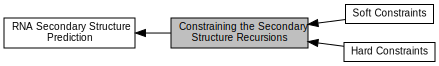
\includegraphics[width=350pt]{group__constraints}
\end{center}
\end{figure}
\subsection*{Modules}
\begin{DoxyCompactItemize}
\item 
\hyperlink{group__hard__constraints}{Hard Constraints}
\item 
\hyperlink{group__soft__constraints}{Soft Constraints}
\end{DoxyCompactItemize}
\subsection*{Macros}
\begin{DoxyCompactItemize}
\item 
\#define \hyperlink{group__constraints_ga13053547a2de5532b64b64d35e097ae1}{V\+R\+N\+A\+\_\+\+C\+O\+N\+S\+T\+R\+A\+I\+N\+T\+\_\+\+D\+B\+\_\+\+P\+I\+P\+E}~1\+U
\begin{DoxyCompactList}\small\item\em Flag that is used to indicate the pipe '$\vert$' sign in pseudo dot-\/bracket notation of hard constraints. \end{DoxyCompactList}\item 
\#define \hyperlink{group__constraints_ga369bea82eae75fbe626f409fa425747e}{V\+R\+N\+A\+\_\+\+C\+O\+N\+S\+T\+R\+A\+I\+N\+T\+\_\+\+D\+B\+\_\+\+D\+O\+T}~2\+U
\begin{DoxyCompactList}\small\item\em dot '.' switch for structure constraints (no constraint at all) \end{DoxyCompactList}\item 
\#define \hyperlink{group__constraints_ga7283bbe0f8954f7b030ecc3f2d1932b2}{V\+R\+N\+A\+\_\+\+C\+O\+N\+S\+T\+R\+A\+I\+N\+T\+\_\+\+D\+B\+\_\+\+X}~4\+U
\begin{DoxyCompactList}\small\item\em 'x' switch for structure constraint (base must not pair) \end{DoxyCompactList}\item 
\#define \hyperlink{group__constraints_gad54c1315a47d55653dcaa5de6e544b77}{V\+R\+N\+A\+\_\+\+C\+O\+N\+S\+T\+R\+A\+I\+N\+T\+\_\+\+D\+B\+\_\+\+A\+N\+G\+\_\+\+B\+R\+A\+C\+K}~8\+U
\begin{DoxyCompactList}\small\item\em angle brackets '$<$', '$>$' switch for structure constraint (paired downstream/upstream) \end{DoxyCompactList}\item 
\#define \hyperlink{group__constraints_gac17b034852c914bc5879954c65d7e74b}{V\+R\+N\+A\+\_\+\+C\+O\+N\+S\+T\+R\+A\+I\+N\+T\+\_\+\+D\+B\+\_\+\+R\+N\+D\+\_\+\+B\+R\+A\+C\+K}~16\+U
\begin{DoxyCompactList}\small\item\em round brackets '(',')' switch for structure constraint (base i pairs base j) \end{DoxyCompactList}\item 
\#define \hyperlink{group__constraints_ga5c17253f5a39d1d49b0fb11f5196982a}{V\+R\+N\+A\+\_\+\+C\+O\+N\+S\+T\+R\+A\+I\+N\+T\+\_\+\+D\+B\+\_\+\+I\+N\+T\+R\+A\+M\+O\+L}~2048\+U
\begin{DoxyCompactList}\small\item\em Flag that is used to indicate the character 'l' in pseudo dot-\/bracket notation of hard constraints. \end{DoxyCompactList}\item 
\#define \hyperlink{group__constraints_ga31d0ebb9755ca8a4acafc14f00ca755d}{V\+R\+N\+A\+\_\+\+C\+O\+N\+S\+T\+R\+A\+I\+N\+T\+\_\+\+D\+B\+\_\+\+I\+N\+T\+E\+R\+M\+O\+L}~4096\+U
\begin{DoxyCompactList}\small\item\em Flag that is used to indicate the character 'e' in pseudo dot-\/bracket notation of hard constraints. \end{DoxyCompactList}\item 
\#define \hyperlink{group__constraints_ga75cfab03cdc97c95b3ce8bb29f52b08e}{V\+R\+N\+A\+\_\+\+C\+O\+N\+S\+T\+R\+A\+I\+N\+T\+\_\+\+D\+B\+\_\+\+G\+Q\+U\+A\+D}~8192\+U
\begin{DoxyCompactList}\small\item\em '+' switch for structure constraint (base is involved in a gquad) \end{DoxyCompactList}\item 
\#define \hyperlink{group__constraints_ga29ebe940110d60ab798fdacbcdbbfb7d}{V\+R\+N\+A\+\_\+\+C\+O\+N\+S\+T\+R\+A\+I\+N\+T\+\_\+\+D\+B\+\_\+\+E\+N\+F\+O\+R\+C\+E\+\_\+\+B\+P}~16384\+U
\begin{DoxyCompactList}\small\item\em Switch for dot-\/bracket structure constraint to enforce base pairs. \end{DoxyCompactList}\item 
\hypertarget{group__constraints_ga0a697f77a6fbb10f34e16fa68ed9e655}{\#define \hyperlink{group__constraints_ga0a697f77a6fbb10f34e16fa68ed9e655}{V\+R\+N\+A\+\_\+\+C\+O\+N\+S\+T\+R\+A\+I\+N\+T\+\_\+\+A\+L\+L}~128\+U}\label{group__constraints_ga0a697f77a6fbb10f34e16fa68ed9e655}

\begin{DoxyCompactList}\small\item\em placeholder for all constraining characters \end{DoxyCompactList}\item 
\#define \hyperlink{group__constraints_ga4bfc2f15c4f261c62a11af9d2aa80c90}{V\+R\+N\+A\+\_\+\+C\+O\+N\+S\+T\+R\+A\+I\+N\+T\+\_\+\+D\+B}~256\+U
\begin{DoxyCompactList}\small\item\em Flag for \hyperlink{group__constraints_ga35a401f680969a556858a8dd5f1d07cc}{vrna\+\_\+constraints\+\_\+add()} to indicate that constraint is passed in pseudo dot-\/bracket notation. \end{DoxyCompactList}\item 
\#define \hyperlink{group__constraints_ga62e0ed0c33002c09423de4e646f85a2b}{V\+R\+N\+A\+\_\+\+C\+O\+N\+S\+T\+R\+A\+I\+N\+T\+\_\+\+F\+I\+L\+E}~512\+U
\begin{DoxyCompactList}\small\item\em Flag for \hyperlink{group__constraints_ga35a401f680969a556858a8dd5f1d07cc}{vrna\+\_\+constraints\+\_\+add()} to indicate that constraints are present in a text file. \end{DoxyCompactList}\end{DoxyCompactItemize}
\subsection*{Typedefs}
\begin{DoxyCompactItemize}
\item 
\hypertarget{group__constraints_gac7e4c4f8abe3163a68110c5bff24e01d}{typedef struct \hyperlink{group__hard__constraints_structvrna__hc__s}{vrna\+\_\+hc\+\_\+s} \hyperlink{group__constraints_gac7e4c4f8abe3163a68110c5bff24e01d}{vrna\+\_\+hc\+\_\+t}}\label{group__constraints_gac7e4c4f8abe3163a68110c5bff24e01d}

\begin{DoxyCompactList}\small\item\em Typename for the hard constraints data structure \hyperlink{group__hard__constraints_structvrna__hc__s}{vrna\+\_\+hc\+\_\+s}. \end{DoxyCompactList}\item 
\hypertarget{group__constraints_ga75401ce219ef8dbcceb672db82d434c6}{typedef struct \hyperlink{group__soft__constraints_structvrna__sc__s}{vrna\+\_\+sc\+\_\+s} \hyperlink{group__constraints_ga75401ce219ef8dbcceb672db82d434c6}{vrna\+\_\+sc\+\_\+t}}\label{group__constraints_ga75401ce219ef8dbcceb672db82d434c6}

\begin{DoxyCompactList}\small\item\em Typename for the soft constraints data structure \hyperlink{group__soft__constraints_structvrna__sc__s}{vrna\+\_\+sc\+\_\+s}. \end{DoxyCompactList}\end{DoxyCompactItemize}
\subsection*{Functions}
\begin{DoxyCompactItemize}
\item 
void \hyperlink{group__constraints_gaa1f20b53bf09ac2e6b0dbb13f7d89670}{vrna\+\_\+message\+\_\+constraint\+\_\+options} (unsigned int option)
\begin{DoxyCompactList}\small\item\em Print a help message for pseudo dot-\/bracket structure constraint characters to stdout. (constraint support is specified by option parameter) \end{DoxyCompactList}\item 
void \hyperlink{group__constraints_gaec7e13fa0465c2acc7a621d1aecb709f}{vrna\+\_\+message\+\_\+constraint\+\_\+options\+\_\+all} (void)
\begin{DoxyCompactList}\small\item\em Print structure constraint characters to stdout (full constraint support) \end{DoxyCompactList}\item 
void \hyperlink{group__constraints_ga35a401f680969a556858a8dd5f1d07cc}{vrna\+\_\+constraints\+\_\+add} (\hyperlink{group__fold__compound_ga1b0cef17fd40466cef5968eaeeff6166}{vrna\+\_\+fold\+\_\+compound\+\_\+t} $\ast$vc, const char $\ast$constraint, unsigned int options)
\begin{DoxyCompactList}\small\item\em Add constraints to a \hyperlink{group__fold__compound_ga1b0cef17fd40466cef5968eaeeff6166}{vrna\+\_\+fold\+\_\+compound\+\_\+t} data structure. \end{DoxyCompactList}\end{DoxyCompactItemize}


\subsection{Detailed Description}
This module covers all functions and variables related to the problem of incorporating secondary structure constraints into the folding recursions. 

This module provides general functions that allow for an easy control of constrained secondary structure prediction and evaluation. Secondary Structure constraints can be subdivided into two groups\+:


\begin{DoxyItemize}
\item \hyperlink{group__hard__constraints}{Hard Constraints}, and
\item \hyperlink{group__soft__constraints}{Soft Constraints}.
\end{DoxyItemize}

While Hard-\/\+Constraints directly influence the production rules used in the folding recursions by allowing, disallowing, or enforcing certain decomposition steps, Soft-\/constraints on the other hand are used to change position specific contributions in the recursions by adding bonuses/penalties in form of pseudo free energies to certain loop configurations. 

\subsection{Macro Definition Documentation}
\hypertarget{group__constraints_ga13053547a2de5532b64b64d35e097ae1}{\index{Constraining the Secondary Structure Recursions@{Constraining the Secondary Structure Recursions}!V\+R\+N\+A\+\_\+\+C\+O\+N\+S\+T\+R\+A\+I\+N\+T\+\_\+\+D\+B\+\_\+\+P\+I\+P\+E@{V\+R\+N\+A\+\_\+\+C\+O\+N\+S\+T\+R\+A\+I\+N\+T\+\_\+\+D\+B\+\_\+\+P\+I\+P\+E}}
\index{V\+R\+N\+A\+\_\+\+C\+O\+N\+S\+T\+R\+A\+I\+N\+T\+\_\+\+D\+B\+\_\+\+P\+I\+P\+E@{V\+R\+N\+A\+\_\+\+C\+O\+N\+S\+T\+R\+A\+I\+N\+T\+\_\+\+D\+B\+\_\+\+P\+I\+P\+E}!Constraining the Secondary Structure Recursions@{Constraining the Secondary Structure Recursions}}
\subsubsection[{V\+R\+N\+A\+\_\+\+C\+O\+N\+S\+T\+R\+A\+I\+N\+T\+\_\+\+D\+B\+\_\+\+P\+I\+P\+E}]{\setlength{\rightskip}{0pt plus 5cm}\#define V\+R\+N\+A\+\_\+\+C\+O\+N\+S\+T\+R\+A\+I\+N\+T\+\_\+\+D\+B\+\_\+\+P\+I\+P\+E~1\+U}}\label{group__constraints_ga13053547a2de5532b64b64d35e097ae1}


{\ttfamily \#include $<$\hyperlink{constraints_8h}{Vienna\+R\+N\+A/constraints.\+h}$>$}



Flag that is used to indicate the pipe '$\vert$' sign in pseudo dot-\/bracket notation of hard constraints. 

Use this definition to indicate the pipe sign '$\vert$' (paired with another base)

\begin{DoxySeeAlso}{See also}
\hyperlink{group__constraints_ga35a401f680969a556858a8dd5f1d07cc}{vrna\+\_\+constraints\+\_\+add()}, \hyperlink{group__constraints_gaa1f20b53bf09ac2e6b0dbb13f7d89670}{vrna\+\_\+message\+\_\+constraint\+\_\+options()}, \hyperlink{group__constraints_gaec7e13fa0465c2acc7a621d1aecb709f}{vrna\+\_\+message\+\_\+constraint\+\_\+options\+\_\+all()} 
\end{DoxySeeAlso}
\hypertarget{group__constraints_ga369bea82eae75fbe626f409fa425747e}{\index{Constraining the Secondary Structure Recursions@{Constraining the Secondary Structure Recursions}!V\+R\+N\+A\+\_\+\+C\+O\+N\+S\+T\+R\+A\+I\+N\+T\+\_\+\+D\+B\+\_\+\+D\+O\+T@{V\+R\+N\+A\+\_\+\+C\+O\+N\+S\+T\+R\+A\+I\+N\+T\+\_\+\+D\+B\+\_\+\+D\+O\+T}}
\index{V\+R\+N\+A\+\_\+\+C\+O\+N\+S\+T\+R\+A\+I\+N\+T\+\_\+\+D\+B\+\_\+\+D\+O\+T@{V\+R\+N\+A\+\_\+\+C\+O\+N\+S\+T\+R\+A\+I\+N\+T\+\_\+\+D\+B\+\_\+\+D\+O\+T}!Constraining the Secondary Structure Recursions@{Constraining the Secondary Structure Recursions}}
\subsubsection[{V\+R\+N\+A\+\_\+\+C\+O\+N\+S\+T\+R\+A\+I\+N\+T\+\_\+\+D\+B\+\_\+\+D\+O\+T}]{\setlength{\rightskip}{0pt plus 5cm}\#define V\+R\+N\+A\+\_\+\+C\+O\+N\+S\+T\+R\+A\+I\+N\+T\+\_\+\+D\+B\+\_\+\+D\+O\+T~2\+U}}\label{group__constraints_ga369bea82eae75fbe626f409fa425747e}


{\ttfamily \#include $<$\hyperlink{constraints_8h}{Vienna\+R\+N\+A/constraints.\+h}$>$}



dot '.' switch for structure constraints (no constraint at all) 

\begin{DoxySeeAlso}{See also}
\hyperlink{group__constraints_ga35a401f680969a556858a8dd5f1d07cc}{vrna\+\_\+constraints\+\_\+add()}, \hyperlink{group__constraints_gaa1f20b53bf09ac2e6b0dbb13f7d89670}{vrna\+\_\+message\+\_\+constraint\+\_\+options()}, \hyperlink{group__constraints_gaec7e13fa0465c2acc7a621d1aecb709f}{vrna\+\_\+message\+\_\+constraint\+\_\+options\+\_\+all()} 
\end{DoxySeeAlso}
\hypertarget{group__constraints_ga7283bbe0f8954f7b030ecc3f2d1932b2}{\index{Constraining the Secondary Structure Recursions@{Constraining the Secondary Structure Recursions}!V\+R\+N\+A\+\_\+\+C\+O\+N\+S\+T\+R\+A\+I\+N\+T\+\_\+\+D\+B\+\_\+\+X@{V\+R\+N\+A\+\_\+\+C\+O\+N\+S\+T\+R\+A\+I\+N\+T\+\_\+\+D\+B\+\_\+\+X}}
\index{V\+R\+N\+A\+\_\+\+C\+O\+N\+S\+T\+R\+A\+I\+N\+T\+\_\+\+D\+B\+\_\+\+X@{V\+R\+N\+A\+\_\+\+C\+O\+N\+S\+T\+R\+A\+I\+N\+T\+\_\+\+D\+B\+\_\+\+X}!Constraining the Secondary Structure Recursions@{Constraining the Secondary Structure Recursions}}
\subsubsection[{V\+R\+N\+A\+\_\+\+C\+O\+N\+S\+T\+R\+A\+I\+N\+T\+\_\+\+D\+B\+\_\+\+X}]{\setlength{\rightskip}{0pt plus 5cm}\#define V\+R\+N\+A\+\_\+\+C\+O\+N\+S\+T\+R\+A\+I\+N\+T\+\_\+\+D\+B\+\_\+\+X~4\+U}}\label{group__constraints_ga7283bbe0f8954f7b030ecc3f2d1932b2}


{\ttfamily \#include $<$\hyperlink{constraints_8h}{Vienna\+R\+N\+A/constraints.\+h}$>$}



'x' switch for structure constraint (base must not pair) 

\begin{DoxySeeAlso}{See also}
\hyperlink{group__constraints_ga35a401f680969a556858a8dd5f1d07cc}{vrna\+\_\+constraints\+\_\+add()}, \hyperlink{group__constraints_gaa1f20b53bf09ac2e6b0dbb13f7d89670}{vrna\+\_\+message\+\_\+constraint\+\_\+options()}, \hyperlink{group__constraints_gaec7e13fa0465c2acc7a621d1aecb709f}{vrna\+\_\+message\+\_\+constraint\+\_\+options\+\_\+all()} 
\end{DoxySeeAlso}
\hypertarget{group__constraints_gad54c1315a47d55653dcaa5de6e544b77}{\index{Constraining the Secondary Structure Recursions@{Constraining the Secondary Structure Recursions}!V\+R\+N\+A\+\_\+\+C\+O\+N\+S\+T\+R\+A\+I\+N\+T\+\_\+\+D\+B\+\_\+\+A\+N\+G\+\_\+\+B\+R\+A\+C\+K@{V\+R\+N\+A\+\_\+\+C\+O\+N\+S\+T\+R\+A\+I\+N\+T\+\_\+\+D\+B\+\_\+\+A\+N\+G\+\_\+\+B\+R\+A\+C\+K}}
\index{V\+R\+N\+A\+\_\+\+C\+O\+N\+S\+T\+R\+A\+I\+N\+T\+\_\+\+D\+B\+\_\+\+A\+N\+G\+\_\+\+B\+R\+A\+C\+K@{V\+R\+N\+A\+\_\+\+C\+O\+N\+S\+T\+R\+A\+I\+N\+T\+\_\+\+D\+B\+\_\+\+A\+N\+G\+\_\+\+B\+R\+A\+C\+K}!Constraining the Secondary Structure Recursions@{Constraining the Secondary Structure Recursions}}
\subsubsection[{V\+R\+N\+A\+\_\+\+C\+O\+N\+S\+T\+R\+A\+I\+N\+T\+\_\+\+D\+B\+\_\+\+A\+N\+G\+\_\+\+B\+R\+A\+C\+K}]{\setlength{\rightskip}{0pt plus 5cm}\#define V\+R\+N\+A\+\_\+\+C\+O\+N\+S\+T\+R\+A\+I\+N\+T\+\_\+\+D\+B\+\_\+\+A\+N\+G\+\_\+\+B\+R\+A\+C\+K~8\+U}}\label{group__constraints_gad54c1315a47d55653dcaa5de6e544b77}


{\ttfamily \#include $<$\hyperlink{constraints_8h}{Vienna\+R\+N\+A/constraints.\+h}$>$}



angle brackets '$<$', '$>$' switch for structure constraint (paired downstream/upstream) 

\begin{DoxySeeAlso}{See also}
\hyperlink{group__constraints_ga35a401f680969a556858a8dd5f1d07cc}{vrna\+\_\+constraints\+\_\+add()}, \hyperlink{group__constraints_gaa1f20b53bf09ac2e6b0dbb13f7d89670}{vrna\+\_\+message\+\_\+constraint\+\_\+options()}, \hyperlink{group__constraints_gaec7e13fa0465c2acc7a621d1aecb709f}{vrna\+\_\+message\+\_\+constraint\+\_\+options\+\_\+all()} 
\end{DoxySeeAlso}
\hypertarget{group__constraints_gac17b034852c914bc5879954c65d7e74b}{\index{Constraining the Secondary Structure Recursions@{Constraining the Secondary Structure Recursions}!V\+R\+N\+A\+\_\+\+C\+O\+N\+S\+T\+R\+A\+I\+N\+T\+\_\+\+D\+B\+\_\+\+R\+N\+D\+\_\+\+B\+R\+A\+C\+K@{V\+R\+N\+A\+\_\+\+C\+O\+N\+S\+T\+R\+A\+I\+N\+T\+\_\+\+D\+B\+\_\+\+R\+N\+D\+\_\+\+B\+R\+A\+C\+K}}
\index{V\+R\+N\+A\+\_\+\+C\+O\+N\+S\+T\+R\+A\+I\+N\+T\+\_\+\+D\+B\+\_\+\+R\+N\+D\+\_\+\+B\+R\+A\+C\+K@{V\+R\+N\+A\+\_\+\+C\+O\+N\+S\+T\+R\+A\+I\+N\+T\+\_\+\+D\+B\+\_\+\+R\+N\+D\+\_\+\+B\+R\+A\+C\+K}!Constraining the Secondary Structure Recursions@{Constraining the Secondary Structure Recursions}}
\subsubsection[{V\+R\+N\+A\+\_\+\+C\+O\+N\+S\+T\+R\+A\+I\+N\+T\+\_\+\+D\+B\+\_\+\+R\+N\+D\+\_\+\+B\+R\+A\+C\+K}]{\setlength{\rightskip}{0pt plus 5cm}\#define V\+R\+N\+A\+\_\+\+C\+O\+N\+S\+T\+R\+A\+I\+N\+T\+\_\+\+D\+B\+\_\+\+R\+N\+D\+\_\+\+B\+R\+A\+C\+K~16\+U}}\label{group__constraints_gac17b034852c914bc5879954c65d7e74b}


{\ttfamily \#include $<$\hyperlink{constraints_8h}{Vienna\+R\+N\+A/constraints.\+h}$>$}



round brackets '(',')' switch for structure constraint (base i pairs base j) 

\begin{DoxySeeAlso}{See also}
\hyperlink{group__constraints_ga35a401f680969a556858a8dd5f1d07cc}{vrna\+\_\+constraints\+\_\+add()}, \hyperlink{group__constraints_gaa1f20b53bf09ac2e6b0dbb13f7d89670}{vrna\+\_\+message\+\_\+constraint\+\_\+options()}, \hyperlink{group__constraints_gaec7e13fa0465c2acc7a621d1aecb709f}{vrna\+\_\+message\+\_\+constraint\+\_\+options\+\_\+all()} 
\end{DoxySeeAlso}
\hypertarget{group__constraints_ga5c17253f5a39d1d49b0fb11f5196982a}{\index{Constraining the Secondary Structure Recursions@{Constraining the Secondary Structure Recursions}!V\+R\+N\+A\+\_\+\+C\+O\+N\+S\+T\+R\+A\+I\+N\+T\+\_\+\+D\+B\+\_\+\+I\+N\+T\+R\+A\+M\+O\+L@{V\+R\+N\+A\+\_\+\+C\+O\+N\+S\+T\+R\+A\+I\+N\+T\+\_\+\+D\+B\+\_\+\+I\+N\+T\+R\+A\+M\+O\+L}}
\index{V\+R\+N\+A\+\_\+\+C\+O\+N\+S\+T\+R\+A\+I\+N\+T\+\_\+\+D\+B\+\_\+\+I\+N\+T\+R\+A\+M\+O\+L@{V\+R\+N\+A\+\_\+\+C\+O\+N\+S\+T\+R\+A\+I\+N\+T\+\_\+\+D\+B\+\_\+\+I\+N\+T\+R\+A\+M\+O\+L}!Constraining the Secondary Structure Recursions@{Constraining the Secondary Structure Recursions}}
\subsubsection[{V\+R\+N\+A\+\_\+\+C\+O\+N\+S\+T\+R\+A\+I\+N\+T\+\_\+\+D\+B\+\_\+\+I\+N\+T\+R\+A\+M\+O\+L}]{\setlength{\rightskip}{0pt plus 5cm}\#define V\+R\+N\+A\+\_\+\+C\+O\+N\+S\+T\+R\+A\+I\+N\+T\+\_\+\+D\+B\+\_\+\+I\+N\+T\+R\+A\+M\+O\+L~2048\+U}}\label{group__constraints_ga5c17253f5a39d1d49b0fb11f5196982a}


{\ttfamily \#include $<$\hyperlink{constraints_8h}{Vienna\+R\+N\+A/constraints.\+h}$>$}



Flag that is used to indicate the character 'l' in pseudo dot-\/bracket notation of hard constraints. 

Use this definition to indicate the usage of 'l' character (intramolecular pairs only)

\begin{DoxySeeAlso}{See also}
\hyperlink{group__constraints_ga35a401f680969a556858a8dd5f1d07cc}{vrna\+\_\+constraints\+\_\+add()}, \hyperlink{group__constraints_gaa1f20b53bf09ac2e6b0dbb13f7d89670}{vrna\+\_\+message\+\_\+constraint\+\_\+options()}, \hyperlink{group__constraints_gaec7e13fa0465c2acc7a621d1aecb709f}{vrna\+\_\+message\+\_\+constraint\+\_\+options\+\_\+all()} 
\end{DoxySeeAlso}
\hypertarget{group__constraints_ga31d0ebb9755ca8a4acafc14f00ca755d}{\index{Constraining the Secondary Structure Recursions@{Constraining the Secondary Structure Recursions}!V\+R\+N\+A\+\_\+\+C\+O\+N\+S\+T\+R\+A\+I\+N\+T\+\_\+\+D\+B\+\_\+\+I\+N\+T\+E\+R\+M\+O\+L@{V\+R\+N\+A\+\_\+\+C\+O\+N\+S\+T\+R\+A\+I\+N\+T\+\_\+\+D\+B\+\_\+\+I\+N\+T\+E\+R\+M\+O\+L}}
\index{V\+R\+N\+A\+\_\+\+C\+O\+N\+S\+T\+R\+A\+I\+N\+T\+\_\+\+D\+B\+\_\+\+I\+N\+T\+E\+R\+M\+O\+L@{V\+R\+N\+A\+\_\+\+C\+O\+N\+S\+T\+R\+A\+I\+N\+T\+\_\+\+D\+B\+\_\+\+I\+N\+T\+E\+R\+M\+O\+L}!Constraining the Secondary Structure Recursions@{Constraining the Secondary Structure Recursions}}
\subsubsection[{V\+R\+N\+A\+\_\+\+C\+O\+N\+S\+T\+R\+A\+I\+N\+T\+\_\+\+D\+B\+\_\+\+I\+N\+T\+E\+R\+M\+O\+L}]{\setlength{\rightskip}{0pt plus 5cm}\#define V\+R\+N\+A\+\_\+\+C\+O\+N\+S\+T\+R\+A\+I\+N\+T\+\_\+\+D\+B\+\_\+\+I\+N\+T\+E\+R\+M\+O\+L~4096\+U}}\label{group__constraints_ga31d0ebb9755ca8a4acafc14f00ca755d}


{\ttfamily \#include $<$\hyperlink{constraints_8h}{Vienna\+R\+N\+A/constraints.\+h}$>$}



Flag that is used to indicate the character 'e' in pseudo dot-\/bracket notation of hard constraints. 

Use this definition to indicate the usage of 'e' character (intermolecular pairs only)

\begin{DoxySeeAlso}{See also}
\hyperlink{group__constraints_ga35a401f680969a556858a8dd5f1d07cc}{vrna\+\_\+constraints\+\_\+add()}, \hyperlink{group__constraints_gaa1f20b53bf09ac2e6b0dbb13f7d89670}{vrna\+\_\+message\+\_\+constraint\+\_\+options()}, \hyperlink{group__constraints_gaec7e13fa0465c2acc7a621d1aecb709f}{vrna\+\_\+message\+\_\+constraint\+\_\+options\+\_\+all()} 
\end{DoxySeeAlso}
\hypertarget{group__constraints_ga75cfab03cdc97c95b3ce8bb29f52b08e}{\index{Constraining the Secondary Structure Recursions@{Constraining the Secondary Structure Recursions}!V\+R\+N\+A\+\_\+\+C\+O\+N\+S\+T\+R\+A\+I\+N\+T\+\_\+\+D\+B\+\_\+\+G\+Q\+U\+A\+D@{V\+R\+N\+A\+\_\+\+C\+O\+N\+S\+T\+R\+A\+I\+N\+T\+\_\+\+D\+B\+\_\+\+G\+Q\+U\+A\+D}}
\index{V\+R\+N\+A\+\_\+\+C\+O\+N\+S\+T\+R\+A\+I\+N\+T\+\_\+\+D\+B\+\_\+\+G\+Q\+U\+A\+D@{V\+R\+N\+A\+\_\+\+C\+O\+N\+S\+T\+R\+A\+I\+N\+T\+\_\+\+D\+B\+\_\+\+G\+Q\+U\+A\+D}!Constraining the Secondary Structure Recursions@{Constraining the Secondary Structure Recursions}}
\subsubsection[{V\+R\+N\+A\+\_\+\+C\+O\+N\+S\+T\+R\+A\+I\+N\+T\+\_\+\+D\+B\+\_\+\+G\+Q\+U\+A\+D}]{\setlength{\rightskip}{0pt plus 5cm}\#define V\+R\+N\+A\+\_\+\+C\+O\+N\+S\+T\+R\+A\+I\+N\+T\+\_\+\+D\+B\+\_\+\+G\+Q\+U\+A\+D~8192\+U}}\label{group__constraints_ga75cfab03cdc97c95b3ce8bb29f52b08e}


{\ttfamily \#include $<$\hyperlink{constraints_8h}{Vienna\+R\+N\+A/constraints.\+h}$>$}



'+' switch for structure constraint (base is involved in a gquad) 

\begin{DoxySeeAlso}{See also}
\hyperlink{group__constraints_ga35a401f680969a556858a8dd5f1d07cc}{vrna\+\_\+constraints\+\_\+add()}, \hyperlink{group__constraints_gaa1f20b53bf09ac2e6b0dbb13f7d89670}{vrna\+\_\+message\+\_\+constraint\+\_\+options()}, \hyperlink{group__constraints_gaec7e13fa0465c2acc7a621d1aecb709f}{vrna\+\_\+message\+\_\+constraint\+\_\+options\+\_\+all()} 
\end{DoxySeeAlso}
\begin{DoxyWarning}{Warning}
This flag is for future purposes only! No implementation recognizes it yet. 
\end{DoxyWarning}
\hypertarget{group__constraints_ga29ebe940110d60ab798fdacbcdbbfb7d}{\index{Constraining the Secondary Structure Recursions@{Constraining the Secondary Structure Recursions}!V\+R\+N\+A\+\_\+\+C\+O\+N\+S\+T\+R\+A\+I\+N\+T\+\_\+\+D\+B\+\_\+\+E\+N\+F\+O\+R\+C\+E\+\_\+\+B\+P@{V\+R\+N\+A\+\_\+\+C\+O\+N\+S\+T\+R\+A\+I\+N\+T\+\_\+\+D\+B\+\_\+\+E\+N\+F\+O\+R\+C\+E\+\_\+\+B\+P}}
\index{V\+R\+N\+A\+\_\+\+C\+O\+N\+S\+T\+R\+A\+I\+N\+T\+\_\+\+D\+B\+\_\+\+E\+N\+F\+O\+R\+C\+E\+\_\+\+B\+P@{V\+R\+N\+A\+\_\+\+C\+O\+N\+S\+T\+R\+A\+I\+N\+T\+\_\+\+D\+B\+\_\+\+E\+N\+F\+O\+R\+C\+E\+\_\+\+B\+P}!Constraining the Secondary Structure Recursions@{Constraining the Secondary Structure Recursions}}
\subsubsection[{V\+R\+N\+A\+\_\+\+C\+O\+N\+S\+T\+R\+A\+I\+N\+T\+\_\+\+D\+B\+\_\+\+E\+N\+F\+O\+R\+C\+E\+\_\+\+B\+P}]{\setlength{\rightskip}{0pt plus 5cm}\#define V\+R\+N\+A\+\_\+\+C\+O\+N\+S\+T\+R\+A\+I\+N\+T\+\_\+\+D\+B\+\_\+\+E\+N\+F\+O\+R\+C\+E\+\_\+\+B\+P~16384\+U}}\label{group__constraints_ga29ebe940110d60ab798fdacbcdbbfb7d}


{\ttfamily \#include $<$\hyperlink{constraints_8h}{Vienna\+R\+N\+A/constraints.\+h}$>$}



Switch for dot-\/bracket structure constraint to enforce base pairs. 

This flag should be used to really enforce base pairs given in dot-\/bracket constraint rather than just weakly-\/enforcing them.

\begin{DoxySeeAlso}{See also}
\hyperlink{group__constraints_ga35a401f680969a556858a8dd5f1d07cc}{vrna\+\_\+constraints\+\_\+add()} 
\end{DoxySeeAlso}
\hypertarget{group__constraints_ga4bfc2f15c4f261c62a11af9d2aa80c90}{\index{Constraining the Secondary Structure Recursions@{Constraining the Secondary Structure Recursions}!V\+R\+N\+A\+\_\+\+C\+O\+N\+S\+T\+R\+A\+I\+N\+T\+\_\+\+D\+B@{V\+R\+N\+A\+\_\+\+C\+O\+N\+S\+T\+R\+A\+I\+N\+T\+\_\+\+D\+B}}
\index{V\+R\+N\+A\+\_\+\+C\+O\+N\+S\+T\+R\+A\+I\+N\+T\+\_\+\+D\+B@{V\+R\+N\+A\+\_\+\+C\+O\+N\+S\+T\+R\+A\+I\+N\+T\+\_\+\+D\+B}!Constraining the Secondary Structure Recursions@{Constraining the Secondary Structure Recursions}}
\subsubsection[{V\+R\+N\+A\+\_\+\+C\+O\+N\+S\+T\+R\+A\+I\+N\+T\+\_\+\+D\+B}]{\setlength{\rightskip}{0pt plus 5cm}\#define V\+R\+N\+A\+\_\+\+C\+O\+N\+S\+T\+R\+A\+I\+N\+T\+\_\+\+D\+B~256\+U}}\label{group__constraints_ga4bfc2f15c4f261c62a11af9d2aa80c90}


{\ttfamily \#include $<$\hyperlink{constraints_8h}{Vienna\+R\+N\+A/constraints.\+h}$>$}



Flag for \hyperlink{group__constraints_ga35a401f680969a556858a8dd5f1d07cc}{vrna\+\_\+constraints\+\_\+add()} to indicate that constraint is passed in pseudo dot-\/bracket notation. 

\begin{DoxySeeAlso}{See also}
\hyperlink{group__constraints_ga35a401f680969a556858a8dd5f1d07cc}{vrna\+\_\+constraints\+\_\+add()}, \hyperlink{group__constraints_gaa1f20b53bf09ac2e6b0dbb13f7d89670}{vrna\+\_\+message\+\_\+constraint\+\_\+options()}, \hyperlink{group__constraints_gaec7e13fa0465c2acc7a621d1aecb709f}{vrna\+\_\+message\+\_\+constraint\+\_\+options\+\_\+all()} 
\end{DoxySeeAlso}
\hypertarget{group__constraints_ga62e0ed0c33002c09423de4e646f85a2b}{\index{Constraining the Secondary Structure Recursions@{Constraining the Secondary Structure Recursions}!V\+R\+N\+A\+\_\+\+C\+O\+N\+S\+T\+R\+A\+I\+N\+T\+\_\+\+F\+I\+L\+E@{V\+R\+N\+A\+\_\+\+C\+O\+N\+S\+T\+R\+A\+I\+N\+T\+\_\+\+F\+I\+L\+E}}
\index{V\+R\+N\+A\+\_\+\+C\+O\+N\+S\+T\+R\+A\+I\+N\+T\+\_\+\+F\+I\+L\+E@{V\+R\+N\+A\+\_\+\+C\+O\+N\+S\+T\+R\+A\+I\+N\+T\+\_\+\+F\+I\+L\+E}!Constraining the Secondary Structure Recursions@{Constraining the Secondary Structure Recursions}}
\subsubsection[{V\+R\+N\+A\+\_\+\+C\+O\+N\+S\+T\+R\+A\+I\+N\+T\+\_\+\+F\+I\+L\+E}]{\setlength{\rightskip}{0pt plus 5cm}\#define V\+R\+N\+A\+\_\+\+C\+O\+N\+S\+T\+R\+A\+I\+N\+T\+\_\+\+F\+I\+L\+E~512\+U}}\label{group__constraints_ga62e0ed0c33002c09423de4e646f85a2b}


{\ttfamily \#include $<$\hyperlink{constraints_8h}{Vienna\+R\+N\+A/constraints.\+h}$>$}



Flag for \hyperlink{group__constraints_ga35a401f680969a556858a8dd5f1d07cc}{vrna\+\_\+constraints\+\_\+add()} to indicate that constraints are present in a text file. 

\begin{DoxySeeAlso}{See also}
\hyperlink{group__constraints_ga35a401f680969a556858a8dd5f1d07cc}{vrna\+\_\+constraints\+\_\+add()} 
\end{DoxySeeAlso}


\subsection{Function Documentation}
\hypertarget{group__constraints_gaa1f20b53bf09ac2e6b0dbb13f7d89670}{\index{Constraining the Secondary Structure Recursions@{Constraining the Secondary Structure Recursions}!vrna\+\_\+message\+\_\+constraint\+\_\+options@{vrna\+\_\+message\+\_\+constraint\+\_\+options}}
\index{vrna\+\_\+message\+\_\+constraint\+\_\+options@{vrna\+\_\+message\+\_\+constraint\+\_\+options}!Constraining the Secondary Structure Recursions@{Constraining the Secondary Structure Recursions}}
\subsubsection[{vrna\+\_\+message\+\_\+constraint\+\_\+options}]{\setlength{\rightskip}{0pt plus 5cm}void vrna\+\_\+message\+\_\+constraint\+\_\+options (
\begin{DoxyParamCaption}
\item[{unsigned int}]{option}
\end{DoxyParamCaption}
)}}\label{group__constraints_gaa1f20b53bf09ac2e6b0dbb13f7d89670}


{\ttfamily \#include $<$\hyperlink{constraints_8h}{Vienna\+R\+N\+A/constraints.\+h}$>$}



Print a help message for pseudo dot-\/bracket structure constraint characters to stdout. (constraint support is specified by option parameter) 

Currently available options are\+:~\newline
\hyperlink{group__constraints_ga13053547a2de5532b64b64d35e097ae1}{V\+R\+N\+A\+\_\+\+C\+O\+N\+S\+T\+R\+A\+I\+N\+T\+\_\+\+D\+B\+\_\+\+P\+I\+P\+E} (paired with another base)~\newline
\hyperlink{group__constraints_ga369bea82eae75fbe626f409fa425747e}{V\+R\+N\+A\+\_\+\+C\+O\+N\+S\+T\+R\+A\+I\+N\+T\+\_\+\+D\+B\+\_\+\+D\+O\+T} (no constraint at all)~\newline
\hyperlink{group__constraints_ga7283bbe0f8954f7b030ecc3f2d1932b2}{V\+R\+N\+A\+\_\+\+C\+O\+N\+S\+T\+R\+A\+I\+N\+T\+\_\+\+D\+B\+\_\+\+X} (base must not pair)~\newline
\hyperlink{group__constraints_gad54c1315a47d55653dcaa5de6e544b77}{V\+R\+N\+A\+\_\+\+C\+O\+N\+S\+T\+R\+A\+I\+N\+T\+\_\+\+D\+B\+\_\+\+A\+N\+G\+\_\+\+B\+R\+A\+C\+K} (paired downstream/upstream)~\newline
\hyperlink{group__constraints_gac17b034852c914bc5879954c65d7e74b}{V\+R\+N\+A\+\_\+\+C\+O\+N\+S\+T\+R\+A\+I\+N\+T\+\_\+\+D\+B\+\_\+\+R\+N\+D\+\_\+\+B\+R\+A\+C\+K} (base i pairs base j)~\newline
 pass a collection of options as one value like this\+: \begin{DoxyVerb}vrna_message_constraints(option_1 | option_2 | option_n) \end{DoxyVerb}


\begin{DoxySeeAlso}{See also}
\hyperlink{group__constraints_gaec7e13fa0465c2acc7a621d1aecb709f}{vrna\+\_\+message\+\_\+constraint\+\_\+options\+\_\+all()}, \hyperlink{group__constraints_ga35a401f680969a556858a8dd5f1d07cc}{vrna\+\_\+constraints\+\_\+add()}, \hyperlink{group__constraints_ga4bfc2f15c4f261c62a11af9d2aa80c90}{V\+R\+N\+A\+\_\+\+C\+O\+N\+S\+T\+R\+A\+I\+N\+T\+\_\+\+D\+B}, \hyperlink{group__constraints_ga13053547a2de5532b64b64d35e097ae1}{V\+R\+N\+A\+\_\+\+C\+O\+N\+S\+T\+R\+A\+I\+N\+T\+\_\+\+D\+B\+\_\+\+P\+I\+P\+E}, \hyperlink{group__constraints_ga369bea82eae75fbe626f409fa425747e}{V\+R\+N\+A\+\_\+\+C\+O\+N\+S\+T\+R\+A\+I\+N\+T\+\_\+\+D\+B\+\_\+\+D\+O\+T}, \hyperlink{group__constraints_ga7283bbe0f8954f7b030ecc3f2d1932b2}{V\+R\+N\+A\+\_\+\+C\+O\+N\+S\+T\+R\+A\+I\+N\+T\+\_\+\+D\+B\+\_\+\+X}, \hyperlink{group__constraints_gad54c1315a47d55653dcaa5de6e544b77}{V\+R\+N\+A\+\_\+\+C\+O\+N\+S\+T\+R\+A\+I\+N\+T\+\_\+\+D\+B\+\_\+\+A\+N\+G\+\_\+\+B\+R\+A\+C\+K}, \hyperlink{group__constraints_gac17b034852c914bc5879954c65d7e74b}{V\+R\+N\+A\+\_\+\+C\+O\+N\+S\+T\+R\+A\+I\+N\+T\+\_\+\+D\+B\+\_\+\+R\+N\+D\+\_\+\+B\+R\+A\+C\+K}, \hyperlink{group__constraints_ga31d0ebb9755ca8a4acafc14f00ca755d}{V\+R\+N\+A\+\_\+\+C\+O\+N\+S\+T\+R\+A\+I\+N\+T\+\_\+\+D\+B\+\_\+\+I\+N\+T\+E\+R\+M\+O\+L}, \hyperlink{group__constraints_ga5c17253f5a39d1d49b0fb11f5196982a}{V\+R\+N\+A\+\_\+\+C\+O\+N\+S\+T\+R\+A\+I\+N\+T\+\_\+\+D\+B\+\_\+\+I\+N\+T\+R\+A\+M\+O\+L}
\end{DoxySeeAlso}

\begin{DoxyParams}{Parameters}
{\em option} & Option switch that tells which constraint help will be printed \\
\hline
\end{DoxyParams}
\hypertarget{group__constraints_gaec7e13fa0465c2acc7a621d1aecb709f}{\index{Constraining the Secondary Structure Recursions@{Constraining the Secondary Structure Recursions}!vrna\+\_\+message\+\_\+constraint\+\_\+options\+\_\+all@{vrna\+\_\+message\+\_\+constraint\+\_\+options\+\_\+all}}
\index{vrna\+\_\+message\+\_\+constraint\+\_\+options\+\_\+all@{vrna\+\_\+message\+\_\+constraint\+\_\+options\+\_\+all}!Constraining the Secondary Structure Recursions@{Constraining the Secondary Structure Recursions}}
\subsubsection[{vrna\+\_\+message\+\_\+constraint\+\_\+options\+\_\+all}]{\setlength{\rightskip}{0pt plus 5cm}void vrna\+\_\+message\+\_\+constraint\+\_\+options\+\_\+all (
\begin{DoxyParamCaption}
\item[{void}]{}
\end{DoxyParamCaption}
)}}\label{group__constraints_gaec7e13fa0465c2acc7a621d1aecb709f}


{\ttfamily \#include $<$\hyperlink{constraints_8h}{Vienna\+R\+N\+A/constraints.\+h}$>$}



Print structure constraint characters to stdout (full constraint support) 

\begin{DoxySeeAlso}{See also}
\hyperlink{group__constraints_gaa1f20b53bf09ac2e6b0dbb13f7d89670}{vrna\+\_\+message\+\_\+constraint\+\_\+options()}, \hyperlink{group__constraints_ga35a401f680969a556858a8dd5f1d07cc}{vrna\+\_\+constraints\+\_\+add()}, \hyperlink{group__constraints_ga4bfc2f15c4f261c62a11af9d2aa80c90}{V\+R\+N\+A\+\_\+\+C\+O\+N\+S\+T\+R\+A\+I\+N\+T\+\_\+\+D\+B}, \hyperlink{group__constraints_ga13053547a2de5532b64b64d35e097ae1}{V\+R\+N\+A\+\_\+\+C\+O\+N\+S\+T\+R\+A\+I\+N\+T\+\_\+\+D\+B\+\_\+\+P\+I\+P\+E}, \hyperlink{group__constraints_ga369bea82eae75fbe626f409fa425747e}{V\+R\+N\+A\+\_\+\+C\+O\+N\+S\+T\+R\+A\+I\+N\+T\+\_\+\+D\+B\+\_\+\+D\+O\+T}, \hyperlink{group__constraints_ga7283bbe0f8954f7b030ecc3f2d1932b2}{V\+R\+N\+A\+\_\+\+C\+O\+N\+S\+T\+R\+A\+I\+N\+T\+\_\+\+D\+B\+\_\+\+X}, \hyperlink{group__constraints_gad54c1315a47d55653dcaa5de6e544b77}{V\+R\+N\+A\+\_\+\+C\+O\+N\+S\+T\+R\+A\+I\+N\+T\+\_\+\+D\+B\+\_\+\+A\+N\+G\+\_\+\+B\+R\+A\+C\+K}, \hyperlink{group__constraints_gac17b034852c914bc5879954c65d7e74b}{V\+R\+N\+A\+\_\+\+C\+O\+N\+S\+T\+R\+A\+I\+N\+T\+\_\+\+D\+B\+\_\+\+R\+N\+D\+\_\+\+B\+R\+A\+C\+K}, \hyperlink{group__constraints_ga31d0ebb9755ca8a4acafc14f00ca755d}{V\+R\+N\+A\+\_\+\+C\+O\+N\+S\+T\+R\+A\+I\+N\+T\+\_\+\+D\+B\+\_\+\+I\+N\+T\+E\+R\+M\+O\+L}, \hyperlink{group__constraints_ga5c17253f5a39d1d49b0fb11f5196982a}{V\+R\+N\+A\+\_\+\+C\+O\+N\+S\+T\+R\+A\+I\+N\+T\+\_\+\+D\+B\+\_\+\+I\+N\+T\+R\+A\+M\+O\+L} 
\end{DoxySeeAlso}
\hypertarget{group__constraints_ga35a401f680969a556858a8dd5f1d07cc}{\index{Constraining the Secondary Structure Recursions@{Constraining the Secondary Structure Recursions}!vrna\+\_\+constraints\+\_\+add@{vrna\+\_\+constraints\+\_\+add}}
\index{vrna\+\_\+constraints\+\_\+add@{vrna\+\_\+constraints\+\_\+add}!Constraining the Secondary Structure Recursions@{Constraining the Secondary Structure Recursions}}
\subsubsection[{vrna\+\_\+constraints\+\_\+add}]{\setlength{\rightskip}{0pt plus 5cm}void vrna\+\_\+constraints\+\_\+add (
\begin{DoxyParamCaption}
\item[{{\bf vrna\+\_\+fold\+\_\+compound\+\_\+t} $\ast$}]{vc, }
\item[{const char $\ast$}]{constraint, }
\item[{unsigned int}]{options}
\end{DoxyParamCaption}
)}}\label{group__constraints_ga35a401f680969a556858a8dd5f1d07cc}


{\ttfamily \#include $<$\hyperlink{constraints_8h}{Vienna\+R\+N\+A/constraints.\+h}$>$}



Add constraints to a \hyperlink{group__fold__compound_ga1b0cef17fd40466cef5968eaeeff6166}{vrna\+\_\+fold\+\_\+compound\+\_\+t} data structure. 

Use this function to add/update the hard/soft constraints The function allows for passing a string 'constraint' that can either be a filename that points to a constraints definition file or it may be a pseudo dot-\/bracket notation indicating hard constraints. Depending on the type of the string the user has to pass \hyperlink{group__constraints_ga62e0ed0c33002c09423de4e646f85a2b}{V\+R\+N\+A\+\_\+\+C\+O\+N\+S\+T\+R\+A\+I\+N\+T\+\_\+\+F\+I\+L\+E} or \hyperlink{group__constraints_ga4bfc2f15c4f261c62a11af9d2aa80c90}{V\+R\+N\+A\+\_\+\+C\+O\+N\+S\+T\+R\+A\+I\+N\+T\+\_\+\+D\+B} in the option parameter, respectively. If none of these to options are passed, no action is performed, other than to guarantee that at least a hard constraints data structure of type \hyperlink{group__constraints_gac7e4c4f8abe3163a68110c5bff24e01d}{vrna\+\_\+hc\+\_\+t} with default values is present in 'vc'. Already existing hard constraints are not touched.

In case, a psuedo dot-\/bracket string is passed as the second argument, the user has to specify, which characters are allowed to be interpreted as constraints by passing the corresponding options via the third parameter.

\begin{DoxySeeAlso}{See also}
\hyperlink{group__hard__constraints_ga36ff456c43bf920629cee5a236e4f0ff}{vrna\+\_\+hc\+\_\+init()}, \hyperlink{group__soft__constraints_ga9d977a1681356778cc66dceafbe5b032}{vrna\+\_\+sc\+\_\+init()}, \hyperlink{group__hard__constraints_gaeb352e3e6ccd2b567bafa451365bb545}{vrna\+\_\+hc\+\_\+add\+\_\+up()}, \hyperlink{group__hard__constraints_gac49305fc5c7d8653c5fbd2de1e1615e2}{vrna\+\_\+hc\+\_\+add\+\_\+bp()}, \hyperlink{group__soft__constraints_ga30f30c8eff9676775a3e831d972b5284}{vrna\+\_\+sc\+\_\+add\+\_\+up()}, \hyperlink{group__soft__constraints_ga86049d4bb0ea8674cae9b6177156b184}{vrna\+\_\+sc\+\_\+add\+\_\+bp()}, \hyperlink{group__soft__constraints_ga57d612b58e1c61dd6cfcb5a843f8f1b3}{vrna\+\_\+sc\+\_\+add\+\_\+\+S\+H\+A\+P\+E\+\_\+deigan()}, \hyperlink{group__soft__constraints_gaf3c65a045060aef5c4e41693d30af58c}{vrna\+\_\+sc\+\_\+add\+\_\+\+S\+H\+A\+P\+E\+\_\+zarringhalam()}, \hyperlink{group__hard__constraints_ga696dcf77887d856c6f21ea266d8b9ca2}{vrna\+\_\+hc\+\_\+free()}, \hyperlink{group__soft__constraints_ga6d55446448d69346fc313b993c4fb3e8}{vrna\+\_\+sc\+\_\+free()}, \hyperlink{group__constraints_ga62e0ed0c33002c09423de4e646f85a2b}{V\+R\+N\+A\+\_\+\+C\+O\+N\+S\+T\+R\+A\+I\+N\+T\+\_\+\+F\+I\+L\+E}, \hyperlink{group__constraints_ga4bfc2f15c4f261c62a11af9d2aa80c90}{V\+R\+N\+A\+\_\+\+C\+O\+N\+S\+T\+R\+A\+I\+N\+T\+\_\+\+D\+B}, \hyperlink{group__constraints_ga13053547a2de5532b64b64d35e097ae1}{V\+R\+N\+A\+\_\+\+C\+O\+N\+S\+T\+R\+A\+I\+N\+T\+\_\+\+D\+B\+\_\+\+P\+I\+P\+E}, \hyperlink{group__constraints_ga369bea82eae75fbe626f409fa425747e}{V\+R\+N\+A\+\_\+\+C\+O\+N\+S\+T\+R\+A\+I\+N\+T\+\_\+\+D\+B\+\_\+\+D\+O\+T}, \hyperlink{group__constraints_ga7283bbe0f8954f7b030ecc3f2d1932b2}{V\+R\+N\+A\+\_\+\+C\+O\+N\+S\+T\+R\+A\+I\+N\+T\+\_\+\+D\+B\+\_\+\+X}, \hyperlink{group__constraints_gad54c1315a47d55653dcaa5de6e544b77}{V\+R\+N\+A\+\_\+\+C\+O\+N\+S\+T\+R\+A\+I\+N\+T\+\_\+\+D\+B\+\_\+\+A\+N\+G\+\_\+\+B\+R\+A\+C\+K}, \hyperlink{group__constraints_gac17b034852c914bc5879954c65d7e74b}{V\+R\+N\+A\+\_\+\+C\+O\+N\+S\+T\+R\+A\+I\+N\+T\+\_\+\+D\+B\+\_\+\+R\+N\+D\+\_\+\+B\+R\+A\+C\+K}, \hyperlink{group__constraints_ga5c17253f5a39d1d49b0fb11f5196982a}{V\+R\+N\+A\+\_\+\+C\+O\+N\+S\+T\+R\+A\+I\+N\+T\+\_\+\+D\+B\+\_\+\+I\+N\+T\+R\+A\+M\+O\+L}, \hyperlink{group__constraints_ga31d0ebb9755ca8a4acafc14f00ca755d}{V\+R\+N\+A\+\_\+\+C\+O\+N\+S\+T\+R\+A\+I\+N\+T\+\_\+\+D\+B\+\_\+\+I\+N\+T\+E\+R\+M\+O\+L}, \hyperlink{group__constraints_ga75cfab03cdc97c95b3ce8bb29f52b08e}{V\+R\+N\+A\+\_\+\+C\+O\+N\+S\+T\+R\+A\+I\+N\+T\+\_\+\+D\+B\+\_\+\+G\+Q\+U\+A\+D}
\end{DoxySeeAlso}

\begin{DoxyParams}{Parameters}
{\em vc} & The fold compound \\
\hline
{\em constraint} & A string with either the filename of the constraint definitions or a pseudo dot-\/bracket notation of the hard constraint. May be N\+U\+L\+L. \\
\hline
{\em options} & The option flags \\
\hline
\end{DoxyParams}

\include{group__hard__constraints}
\hypertarget{group__soft__constraints}{\section{Soft Constraints}
\label{group__soft__constraints}\index{Soft Constraints@{Soft Constraints}}
}
Collaboration diagram for Soft Constraints\+:
\nopagebreak
\begin{figure}[H]
\begin{center}
\leavevmode
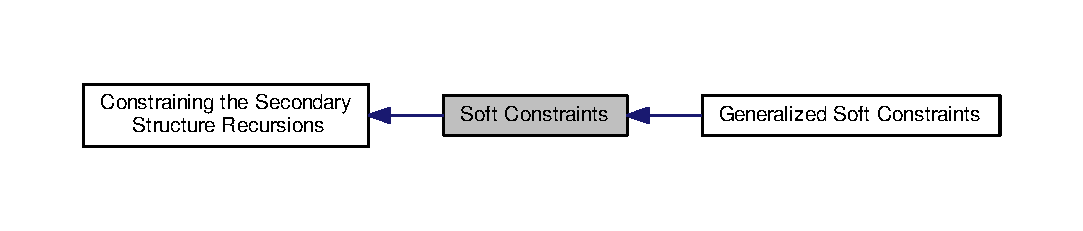
\includegraphics[width=350pt]{group__soft__constraints}
\end{center}
\end{figure}
\subsection*{Modules}
\begin{DoxyCompactItemize}
\item 
\hyperlink{group__generalized__sc}{Generalized Soft Constraints}
\end{DoxyCompactItemize}
\subsection*{Files}
\begin{DoxyCompactItemize}
\item 
file \hyperlink{ligand_8h}{ligand.\+h}
\end{DoxyCompactItemize}
\subsection*{Data Structures}
\begin{DoxyCompactItemize}
\item 
struct \hyperlink{group__soft__constraints_structvrna__sc__s}{vrna\+\_\+sc\+\_\+s}
\begin{DoxyCompactList}\small\item\em The soft constraints data structure.  \hyperlink{group__soft__constraints_structvrna__sc__s}{More...}\end{DoxyCompactList}\end{DoxyCompactItemize}
\subsection*{Macros}
\begin{DoxyCompactItemize}
\item 
\hypertarget{group__soft__constraints_ga62aa195893d02d1a79ca94952748df36}{\#define \hyperlink{group__soft__constraints_ga62aa195893d02d1a79ca94952748df36}{V\+R\+N\+A\+\_\+\+C\+O\+N\+S\+T\+R\+A\+I\+N\+T\+\_\+\+S\+O\+F\+T\+\_\+\+M\+F\+E}~8192\+U}\label{group__soft__constraints_ga62aa195893d02d1a79ca94952748df36}

\begin{DoxyCompactList}\small\item\em Soft constraints flag, apply constraints for M\+F\+E calculations. \end{DoxyCompactList}\item 
\hypertarget{group__soft__constraints_ga03fb5000c19b9a2082bf4ea30a543045}{\#define \hyperlink{group__soft__constraints_ga03fb5000c19b9a2082bf4ea30a543045}{V\+R\+N\+A\+\_\+\+C\+O\+N\+S\+T\+R\+A\+I\+N\+T\+\_\+\+S\+O\+F\+T\+\_\+\+P\+F}~16384\+U}\label{group__soft__constraints_ga03fb5000c19b9a2082bf4ea30a543045}

\begin{DoxyCompactList}\small\item\em Soft constraints flag, apply constraints for partition function calculations. \end{DoxyCompactList}\item 
\#define \hyperlink{group__soft__constraints_ga81e10993d1ae728e4e02022b33155a12}{V\+R\+N\+A\+\_\+\+O\+B\+J\+E\+C\+T\+I\+V\+E\+\_\+\+F\+U\+N\+C\+T\+I\+O\+N\+\_\+\+Q\+U\+A\+D\+R\+A\+T\+I\+C}~0
\begin{DoxyCompactList}\small\item\em Use the sum of squared aberrations as objective function. \end{DoxyCompactList}\item 
\#define \hyperlink{group__soft__constraints_gac070dfb9cafaeb14d5652bd9adf0f6b1}{V\+R\+N\+A\+\_\+\+O\+B\+J\+E\+C\+T\+I\+V\+E\+\_\+\+F\+U\+N\+C\+T\+I\+O\+N\+\_\+\+A\+B\+S\+O\+L\+U\+T\+E}~1
\begin{DoxyCompactList}\small\item\em Use the sum of absolute aberrations as objective function. \end{DoxyCompactList}\item 
\hypertarget{group__soft__constraints_gae5126200d80dbb282f46083fffc606bf}{\#define \hyperlink{group__soft__constraints_gae5126200d80dbb282f46083fffc606bf}{V\+R\+N\+A\+\_\+\+M\+I\+N\+I\+M\+I\+Z\+E\+R\+\_\+\+D\+E\+F\+A\+U\+L\+T}~0}\label{group__soft__constraints_gae5126200d80dbb282f46083fffc606bf}

\begin{DoxyCompactList}\small\item\em Use a custom implementation of the gradient descent algorithm to minimize the objective function. \end{DoxyCompactList}\item 
\#define \hyperlink{group__soft__constraints_gab1d89db58e8c497795a5005f5dbc8c4a}{V\+R\+N\+A\+\_\+\+M\+I\+N\+I\+M\+I\+Z\+E\+R\+\_\+\+C\+O\+N\+J\+U\+G\+A\+T\+E\+\_\+\+F\+R}~1
\begin{DoxyCompactList}\small\item\em Use the G\+N\+U Scientific Library implementation of the Fletcher-\/\+Reeves conjugate gradient algorithm to minimize the objective function. \end{DoxyCompactList}\item 
\#define \hyperlink{group__soft__constraints_ga5aaeafe1b0aa77a5cda18943ff94b02f}{V\+R\+N\+A\+\_\+\+M\+I\+N\+I\+M\+I\+Z\+E\+R\+\_\+\+C\+O\+N\+J\+U\+G\+A\+T\+E\+\_\+\+P\+R}~2
\begin{DoxyCompactList}\small\item\em Use the G\+N\+U Scientific Library implementation of the Polak-\/\+Ribiere conjugate gradient algorithm to minimize the objective function. \end{DoxyCompactList}\item 
\#define \hyperlink{group__soft__constraints_ga9be8a702cddf58235571ace11cc41b22}{V\+R\+N\+A\+\_\+\+M\+I\+N\+I\+M\+I\+Z\+E\+R\+\_\+\+V\+E\+C\+T\+O\+R\+\_\+\+B\+F\+G\+S}~3
\begin{DoxyCompactList}\small\item\em Use the G\+N\+U Scientific Library implementation of the vector Broyden-\/\+Fletcher-\/\+Goldfarb-\/\+Shanno algorithm to minimize the objective function. \end{DoxyCompactList}\item 
\#define \hyperlink{group__soft__constraints_ga7b0a65c6c92fa1d8012383ba9d3dcb4f}{V\+R\+N\+A\+\_\+\+M\+I\+N\+I\+M\+I\+Z\+E\+R\+\_\+\+V\+E\+C\+T\+O\+R\+\_\+\+B\+F\+G\+S2}~4
\begin{DoxyCompactList}\small\item\em Use the G\+N\+U Scientific Library implementation of the vector Broyden-\/\+Fletcher-\/\+Goldfarb-\/\+Shanno algorithm to minimize the objective function. \end{DoxyCompactList}\item 
\#define \hyperlink{group__soft__constraints_ga9ecd2144c2ebed7533233da3986521b0}{V\+R\+N\+A\+\_\+\+M\+I\+N\+I\+M\+I\+Z\+E\+R\+\_\+\+S\+T\+E\+E\+P\+E\+S\+T\+\_\+\+D\+E\+S\+C\+E\+N\+T}~5
\begin{DoxyCompactList}\small\item\em Use the G\+N\+U Scientific Library implementation of the steepest descent algorithm to minimize the objective function. \end{DoxyCompactList}\end{DoxyCompactItemize}
\subsection*{Typedefs}
\begin{DoxyCompactItemize}
\item 
typedef void($\ast$ \hyperlink{group__soft__constraints_gafd57325a0fa4307cd72f933107f9d493}{progress\+\_\+callback} )(int iteration, double score, double $\ast$epsilon)
\begin{DoxyCompactList}\small\item\em Callback for following the progress of the minimization process. \end{DoxyCompactList}\end{DoxyCompactItemize}
\subsection*{Functions}
\begin{DoxyCompactItemize}
\item 
void \hyperlink{group__soft__constraints_ga9d977a1681356778cc66dceafbe5b032}{vrna\+\_\+sc\+\_\+init} (\hyperlink{group__fold__compound_ga1b0cef17fd40466cef5968eaeeff6166}{vrna\+\_\+fold\+\_\+compound\+\_\+t} $\ast$vc)
\begin{DoxyCompactList}\small\item\em Initialize an empty soft constraints data structure within a \hyperlink{group__fold__compound_ga1b0cef17fd40466cef5968eaeeff6166}{vrna\+\_\+fold\+\_\+compound\+\_\+t}. \end{DoxyCompactList}\item 
void \hyperlink{group__soft__constraints_ga86049d4bb0ea8674cae9b6177156b184}{vrna\+\_\+sc\+\_\+add\+\_\+bp} (\hyperlink{group__fold__compound_ga1b0cef17fd40466cef5968eaeeff6166}{vrna\+\_\+fold\+\_\+compound\+\_\+t} $\ast$vc, const \hyperlink{group__data__structures_ga31125aeace516926bf7f251f759b6126}{F\+L\+T\+\_\+\+O\+R\+\_\+\+D\+B\+L} $\ast$$\ast$constraints, unsigned int options)
\begin{DoxyCompactList}\small\item\em Add soft constraints for paired nucleotides. \end{DoxyCompactList}\item 
void \hyperlink{group__soft__constraints_ga30f30c8eff9676775a3e831d972b5284}{vrna\+\_\+sc\+\_\+add\+\_\+up} (\hyperlink{group__fold__compound_ga1b0cef17fd40466cef5968eaeeff6166}{vrna\+\_\+fold\+\_\+compound\+\_\+t} $\ast$vc, const \hyperlink{group__data__structures_ga31125aeace516926bf7f251f759b6126}{F\+L\+T\+\_\+\+O\+R\+\_\+\+D\+B\+L} $\ast$constraints, unsigned int options)
\begin{DoxyCompactList}\small\item\em Add soft constraints for unpaired nucleotides. \end{DoxyCompactList}\item 
void \hyperlink{group__soft__constraints_ga73cdc07b9a199c614367bebef0f2c41a}{vrna\+\_\+sc\+\_\+remove} (\hyperlink{group__fold__compound_ga1b0cef17fd40466cef5968eaeeff6166}{vrna\+\_\+fold\+\_\+compound\+\_\+t} $\ast$vc)
\begin{DoxyCompactList}\small\item\em Remove soft constraints from \hyperlink{group__fold__compound_ga1b0cef17fd40466cef5968eaeeff6166}{vrna\+\_\+fold\+\_\+compound\+\_\+t}. \end{DoxyCompactList}\item 
void \hyperlink{group__soft__constraints_ga6d55446448d69346fc313b993c4fb3e8}{vrna\+\_\+sc\+\_\+free} (\hyperlink{group__constraints_ga75401ce219ef8dbcceb672db82d434c6}{vrna\+\_\+sc\+\_\+t} $\ast$sc)
\begin{DoxyCompactList}\small\item\em Free memory occupied by a \hyperlink{group__constraints_ga75401ce219ef8dbcceb672db82d434c6}{vrna\+\_\+sc\+\_\+t} data structure. \end{DoxyCompactList}\item 
int \hyperlink{group__soft__constraints_ga57d612b58e1c61dd6cfcb5a843f8f1b3}{vrna\+\_\+sc\+\_\+add\+\_\+\+S\+H\+A\+P\+E\+\_\+deigan} (\hyperlink{group__fold__compound_ga1b0cef17fd40466cef5968eaeeff6166}{vrna\+\_\+fold\+\_\+compound\+\_\+t} $\ast$vc, const double $\ast$reactivities, double m, double b, unsigned int options)
\begin{DoxyCompactList}\small\item\em Add S\+H\+A\+P\+E reactivity data as soft constraints (Deigan et al. method) \end{DoxyCompactList}\item 
int \hyperlink{group__soft__constraints_ga04ba85da63d8c793bb8001d1e6f800ba}{vrna\+\_\+sc\+\_\+add\+\_\+\+S\+H\+A\+P\+E\+\_\+deigan\+\_\+ali} (\hyperlink{group__fold__compound_ga1b0cef17fd40466cef5968eaeeff6166}{vrna\+\_\+fold\+\_\+compound\+\_\+t} $\ast$vc, const char $\ast$$\ast$shape\+\_\+files, const int $\ast$shape\+\_\+file\+\_\+association, double m, double b, unsigned int options)
\begin{DoxyCompactList}\small\item\em Add S\+H\+A\+P\+E reactivity data from files as soft constraints for consensus structure prediction (Deigan et al. method) \end{DoxyCompactList}\item 
int \hyperlink{group__soft__constraints_gaf3c65a045060aef5c4e41693d30af58c}{vrna\+\_\+sc\+\_\+add\+\_\+\+S\+H\+A\+P\+E\+\_\+zarringhalam} (\hyperlink{group__fold__compound_ga1b0cef17fd40466cef5968eaeeff6166}{vrna\+\_\+fold\+\_\+compound\+\_\+t} $\ast$vc, const double $\ast$reactivities, double b, double default\+\_\+value, const char $\ast$shape\+\_\+conversion, unsigned int options)
\begin{DoxyCompactList}\small\item\em Add S\+H\+A\+P\+E reactivity data as soft constraints (Zarringhalam et al. method) \end{DoxyCompactList}\item 
int \hyperlink{group__soft__constraints_ga67675b3ed48744489a3bcfa4174197cb}{vrna\+\_\+sc\+\_\+\+S\+H\+A\+P\+E\+\_\+to\+\_\+pr} (const char $\ast$shape\+\_\+conversion, double $\ast$values, int length, double default\+\_\+value)
\begin{DoxyCompactList}\small\item\em Convert S\+H\+A\+P\+E reactivity values to probabilities for being unpaired. \end{DoxyCompactList}\item 
void \hyperlink{group__soft__constraints_gaa124bdc20d88001c38ade590c4bcc3c4}{vrna\+\_\+sc\+\_\+minimize\+\_\+pertubation} (\hyperlink{group__fold__compound_ga1b0cef17fd40466cef5968eaeeff6166}{vrna\+\_\+fold\+\_\+compound\+\_\+t} $\ast$vc, const double $\ast$q\+\_\+prob\+\_\+unpaired, int objective\+\_\+function, double sigma\+\_\+squared, double tau\+\_\+squared, int algorithm, int sample\+\_\+size, double $\ast$epsilon, double initial\+Step\+Size, double min\+Step\+Size, double min\+Improvement, double minimizer\+Tolerance, \hyperlink{group__soft__constraints_gafd57325a0fa4307cd72f933107f9d493}{progress\+\_\+callback} callback)
\begin{DoxyCompactList}\small\item\em Find a vector of perturbation energies that minimizes the discripancies between predicted and observed pairing probabilities and the amount of neccessary adjustments. \end{DoxyCompactList}\end{DoxyCompactItemize}


\subsection{Detailed Description}


\subsection{Data Structure Documentation}
\index{vrna\+\_\+sc\+\_\+s@{vrna\+\_\+sc\+\_\+s}}\label{structvrna__sc__s}
\hypertarget{group__soft__constraints_structvrna__sc__s}{}
\subsubsection{struct vrna\+\_\+sc\+\_\+s}
The soft constraints data structure. \subsubsection*{Data Fields}
\begin{DoxyCompactItemize}
\item 
\hypertarget{group__soft__constraints_a57e4dbb924ab11f304e3762a3a9b07a1}{int $\ast$$\ast$ \hyperlink{group__soft__constraints_a57e4dbb924ab11f304e3762a3a9b07a1}{energy\+\_\+up}}\label{group__soft__constraints_a57e4dbb924ab11f304e3762a3a9b07a1}

\begin{DoxyCompactList}\small\item\em Energy contribution for stretches of unpaired nucleotides. \end{DoxyCompactList}\item 
\hypertarget{group__soft__constraints_ad139b8e06632e00cbcf3909815d0d03d}{int $\ast$ \hyperlink{group__soft__constraints_ad139b8e06632e00cbcf3909815d0d03d}{energy\+\_\+bp}}\label{group__soft__constraints_ad139b8e06632e00cbcf3909815d0d03d}

\begin{DoxyCompactList}\small\item\em Energy contribution for base pairs. \end{DoxyCompactList}\item 
\hypertarget{group__soft__constraints_ad3b4972d3b6c23865587e4ac56a37375}{\hyperlink{group__data__structures_ga31125aeace516926bf7f251f759b6126}{F\+L\+T\+\_\+\+O\+R\+\_\+\+D\+B\+L} $\ast$$\ast$ \hyperlink{group__soft__constraints_ad3b4972d3b6c23865587e4ac56a37375}{exp\+\_\+energy\+\_\+up}}\label{group__soft__constraints_ad3b4972d3b6c23865587e4ac56a37375}

\begin{DoxyCompactList}\small\item\em Boltzmann Factors of the energy contributions for unpaired sequence stretches. \end{DoxyCompactList}\item 
\hypertarget{group__soft__constraints_a62c22be478cd630541c91f73e6cb0d75}{\hyperlink{group__data__structures_ga31125aeace516926bf7f251f759b6126}{F\+L\+T\+\_\+\+O\+R\+\_\+\+D\+B\+L} $\ast$ \hyperlink{group__soft__constraints_a62c22be478cd630541c91f73e6cb0d75}{exp\+\_\+energy\+\_\+bp}}\label{group__soft__constraints_a62c22be478cd630541c91f73e6cb0d75}

\begin{DoxyCompactList}\small\item\em Boltzmann Factors of the energy contribution for base pairs. \end{DoxyCompactList}\item 
\hypertarget{group__soft__constraints_ac20dded6068e81acd0f1139092f66a22}{int $\ast$ \hyperlink{group__soft__constraints_ac20dded6068e81acd0f1139092f66a22}{energy\+\_\+stack}}\label{group__soft__constraints_ac20dded6068e81acd0f1139092f66a22}

\begin{DoxyCompactList}\small\item\em Pseudo Energy contribution per base pair involved in a stack. \end{DoxyCompactList}\item 
\hypertarget{group__soft__constraints_a4a0058fe3d5ba3416f0aaab677610115}{\hyperlink{group__data__structures_ga31125aeace516926bf7f251f759b6126}{F\+L\+T\+\_\+\+O\+R\+\_\+\+D\+B\+L} $\ast$ \hyperlink{group__soft__constraints_a4a0058fe3d5ba3416f0aaab677610115}{exp\+\_\+energy\+\_\+stack}}\label{group__soft__constraints_a4a0058fe3d5ba3416f0aaab677610115}

\begin{DoxyCompactList}\small\item\em Boltzmann weighted pseudo energy contribution per nucleotide involved in a stack. \end{DoxyCompactList}\item 
\hyperlink{group__generalized__sc_ga2f3d2d2333e5a616e0f5cd4823780c0c}{vrna\+\_\+callback\+\_\+sc\+\_\+energy} $\ast$ \hyperlink{group__soft__constraints_a32dc86090237888c75491bbd4861a04b}{f}
\begin{DoxyCompactList}\small\item\em A function pointer used for pseudo energy contribution in M\+F\+E calculations. \end{DoxyCompactList}\item 
\hyperlink{group__generalized__sc_ga1157aec50aa078464b868b5d2245ebf5}{vrna\+\_\+callback\+\_\+sc\+\_\+backtrack} $\ast$ \hyperlink{group__soft__constraints_a2a2aca01782c2b980d7b7fd05b9be89c}{bt}
\begin{DoxyCompactList}\small\item\em A function pointer used to obtain backtraced base pairs in loop regions that were altered by soft constrained pseudo energy contributions. \end{DoxyCompactList}\item 
\hyperlink{group__generalized__sc_ga28d5138cc47eb7a5116c87518fd076a9}{vrna\+\_\+callback\+\_\+sc\+\_\+exp\+\_\+energy} $\ast$ \hyperlink{group__soft__constraints_a0de08a09f3ccf2f97974d23192668ab0}{exp\+\_\+f}
\begin{DoxyCompactList}\small\item\em A function pointer used for pseudo energy contribution boltzmann factors in P\+F calculations. \end{DoxyCompactList}\item 
\hypertarget{group__soft__constraints_a7574680143df97b9029146c2150bf06d}{void $\ast$ \hyperlink{group__soft__constraints_a7574680143df97b9029146c2150bf06d}{data}}\label{group__soft__constraints_a7574680143df97b9029146c2150bf06d}

\begin{DoxyCompactList}\small\item\em A pointer to the data object provided for for pseudo energy contribution functions of the generalized soft constraints feature. \end{DoxyCompactList}\end{DoxyCompactItemize}


\paragraph{Field Documentation}
\hypertarget{group__soft__constraints_a32dc86090237888c75491bbd4861a04b}{\index{vrna\+\_\+sc\+\_\+s@{vrna\+\_\+sc\+\_\+s}!f@{f}}
\index{f@{f}!vrna\+\_\+sc\+\_\+s@{vrna\+\_\+sc\+\_\+s}}
\subparagraph[{f}]{\setlength{\rightskip}{0pt plus 5cm}{\bf vrna\+\_\+callback\+\_\+sc\+\_\+energy}$\ast$ vrna\+\_\+sc\+\_\+s\+::f}}\label{group__soft__constraints_a32dc86090237888c75491bbd4861a04b}


A function pointer used for pseudo energy contribution in M\+F\+E calculations. 

\begin{DoxySeeAlso}{See also}
\hyperlink{group__generalized__sc_ga8c7d907ec0125cd61c04e0908010a4e9}{vrna\+\_\+sc\+\_\+add\+\_\+f()} 
\end{DoxySeeAlso}
\hypertarget{group__soft__constraints_a2a2aca01782c2b980d7b7fd05b9be89c}{\index{vrna\+\_\+sc\+\_\+s@{vrna\+\_\+sc\+\_\+s}!bt@{bt}}
\index{bt@{bt}!vrna\+\_\+sc\+\_\+s@{vrna\+\_\+sc\+\_\+s}}
\subparagraph[{bt}]{\setlength{\rightskip}{0pt plus 5cm}{\bf vrna\+\_\+callback\+\_\+sc\+\_\+backtrack}$\ast$ vrna\+\_\+sc\+\_\+s\+::bt}}\label{group__soft__constraints_a2a2aca01782c2b980d7b7fd05b9be89c}


A function pointer used to obtain backtraced base pairs in loop regions that were altered by soft constrained pseudo energy contributions. 

\begin{DoxySeeAlso}{See also}
\hyperlink{group__generalized__sc_gabde7d07a79bb9a8f4721aee247b674ea}{vrna\+\_\+sc\+\_\+add\+\_\+bt()} 
\end{DoxySeeAlso}
\hypertarget{group__soft__constraints_a0de08a09f3ccf2f97974d23192668ab0}{\index{vrna\+\_\+sc\+\_\+s@{vrna\+\_\+sc\+\_\+s}!exp\+\_\+f@{exp\+\_\+f}}
\index{exp\+\_\+f@{exp\+\_\+f}!vrna\+\_\+sc\+\_\+s@{vrna\+\_\+sc\+\_\+s}}
\subparagraph[{exp\+\_\+f}]{\setlength{\rightskip}{0pt plus 5cm}{\bf vrna\+\_\+callback\+\_\+sc\+\_\+exp\+\_\+energy}$\ast$ vrna\+\_\+sc\+\_\+s\+::exp\+\_\+f}}\label{group__soft__constraints_a0de08a09f3ccf2f97974d23192668ab0}


A function pointer used for pseudo energy contribution boltzmann factors in P\+F calculations. 

\begin{DoxySeeAlso}{See also}
\hyperlink{group__generalized__sc_ga87e382b5d0c9b7d9ce1b79c0473ff700}{vrna\+\_\+sc\+\_\+add\+\_\+exp\+\_\+f()} 
\end{DoxySeeAlso}


\subsection{Macro Definition Documentation}
\hypertarget{group__soft__constraints_ga81e10993d1ae728e4e02022b33155a12}{\index{Soft Constraints@{Soft Constraints}!V\+R\+N\+A\+\_\+\+O\+B\+J\+E\+C\+T\+I\+V\+E\+\_\+\+F\+U\+N\+C\+T\+I\+O\+N\+\_\+\+Q\+U\+A\+D\+R\+A\+T\+I\+C@{V\+R\+N\+A\+\_\+\+O\+B\+J\+E\+C\+T\+I\+V\+E\+\_\+\+F\+U\+N\+C\+T\+I\+O\+N\+\_\+\+Q\+U\+A\+D\+R\+A\+T\+I\+C}}
\index{V\+R\+N\+A\+\_\+\+O\+B\+J\+E\+C\+T\+I\+V\+E\+\_\+\+F\+U\+N\+C\+T\+I\+O\+N\+\_\+\+Q\+U\+A\+D\+R\+A\+T\+I\+C@{V\+R\+N\+A\+\_\+\+O\+B\+J\+E\+C\+T\+I\+V\+E\+\_\+\+F\+U\+N\+C\+T\+I\+O\+N\+\_\+\+Q\+U\+A\+D\+R\+A\+T\+I\+C}!Soft Constraints@{Soft Constraints}}
\subsubsection[{V\+R\+N\+A\+\_\+\+O\+B\+J\+E\+C\+T\+I\+V\+E\+\_\+\+F\+U\+N\+C\+T\+I\+O\+N\+\_\+\+Q\+U\+A\+D\+R\+A\+T\+I\+C}]{\setlength{\rightskip}{0pt plus 5cm}\#define V\+R\+N\+A\+\_\+\+O\+B\+J\+E\+C\+T\+I\+V\+E\+\_\+\+F\+U\+N\+C\+T\+I\+O\+N\+\_\+\+Q\+U\+A\+D\+R\+A\+T\+I\+C~0}}\label{group__soft__constraints_ga81e10993d1ae728e4e02022b33155a12}


{\ttfamily \#include $<$Vienna\+R\+N\+A/perturbation\+\_\+fold.\+h$>$}



Use the sum of squared aberrations as objective function. 

$ F(\vec\epsilon) = \sum_{i = 1}^n{ \frac{\epsilon_i^2}{\tau^2} } + \sum_{i = 1}^n{ \frac{(p_i(\vec\epsilon) - q_i)^2}{\sigma^2} } \to min $ \hypertarget{group__soft__constraints_gac070dfb9cafaeb14d5652bd9adf0f6b1}{\index{Soft Constraints@{Soft Constraints}!V\+R\+N\+A\+\_\+\+O\+B\+J\+E\+C\+T\+I\+V\+E\+\_\+\+F\+U\+N\+C\+T\+I\+O\+N\+\_\+\+A\+B\+S\+O\+L\+U\+T\+E@{V\+R\+N\+A\+\_\+\+O\+B\+J\+E\+C\+T\+I\+V\+E\+\_\+\+F\+U\+N\+C\+T\+I\+O\+N\+\_\+\+A\+B\+S\+O\+L\+U\+T\+E}}
\index{V\+R\+N\+A\+\_\+\+O\+B\+J\+E\+C\+T\+I\+V\+E\+\_\+\+F\+U\+N\+C\+T\+I\+O\+N\+\_\+\+A\+B\+S\+O\+L\+U\+T\+E@{V\+R\+N\+A\+\_\+\+O\+B\+J\+E\+C\+T\+I\+V\+E\+\_\+\+F\+U\+N\+C\+T\+I\+O\+N\+\_\+\+A\+B\+S\+O\+L\+U\+T\+E}!Soft Constraints@{Soft Constraints}}
\subsubsection[{V\+R\+N\+A\+\_\+\+O\+B\+J\+E\+C\+T\+I\+V\+E\+\_\+\+F\+U\+N\+C\+T\+I\+O\+N\+\_\+\+A\+B\+S\+O\+L\+U\+T\+E}]{\setlength{\rightskip}{0pt plus 5cm}\#define V\+R\+N\+A\+\_\+\+O\+B\+J\+E\+C\+T\+I\+V\+E\+\_\+\+F\+U\+N\+C\+T\+I\+O\+N\+\_\+\+A\+B\+S\+O\+L\+U\+T\+E~1}}\label{group__soft__constraints_gac070dfb9cafaeb14d5652bd9adf0f6b1}


{\ttfamily \#include $<$Vienna\+R\+N\+A/perturbation\+\_\+fold.\+h$>$}



Use the sum of absolute aberrations as objective function. 

$ F(\vec\epsilon) = \sum_{i = 1}^n{ \frac{|\epsilon_i|}{\tau^2} } + \sum_{i = 1}^n{ \frac{|p_i(\vec\epsilon) - q_i|}{\sigma^2} } \to min $ \hypertarget{group__soft__constraints_gab1d89db58e8c497795a5005f5dbc8c4a}{\index{Soft Constraints@{Soft Constraints}!V\+R\+N\+A\+\_\+\+M\+I\+N\+I\+M\+I\+Z\+E\+R\+\_\+\+C\+O\+N\+J\+U\+G\+A\+T\+E\+\_\+\+F\+R@{V\+R\+N\+A\+\_\+\+M\+I\+N\+I\+M\+I\+Z\+E\+R\+\_\+\+C\+O\+N\+J\+U\+G\+A\+T\+E\+\_\+\+F\+R}}
\index{V\+R\+N\+A\+\_\+\+M\+I\+N\+I\+M\+I\+Z\+E\+R\+\_\+\+C\+O\+N\+J\+U\+G\+A\+T\+E\+\_\+\+F\+R@{V\+R\+N\+A\+\_\+\+M\+I\+N\+I\+M\+I\+Z\+E\+R\+\_\+\+C\+O\+N\+J\+U\+G\+A\+T\+E\+\_\+\+F\+R}!Soft Constraints@{Soft Constraints}}
\subsubsection[{V\+R\+N\+A\+\_\+\+M\+I\+N\+I\+M\+I\+Z\+E\+R\+\_\+\+C\+O\+N\+J\+U\+G\+A\+T\+E\+\_\+\+F\+R}]{\setlength{\rightskip}{0pt plus 5cm}\#define V\+R\+N\+A\+\_\+\+M\+I\+N\+I\+M\+I\+Z\+E\+R\+\_\+\+C\+O\+N\+J\+U\+G\+A\+T\+E\+\_\+\+F\+R~1}}\label{group__soft__constraints_gab1d89db58e8c497795a5005f5dbc8c4a}


{\ttfamily \#include $<$Vienna\+R\+N\+A/perturbation\+\_\+fold.\+h$>$}



Use the G\+N\+U Scientific Library implementation of the Fletcher-\/\+Reeves conjugate gradient algorithm to minimize the objective function. 

Please note that this algorithm can only be used when the G\+N\+U Scientific Library is available on your system \hypertarget{group__soft__constraints_ga5aaeafe1b0aa77a5cda18943ff94b02f}{\index{Soft Constraints@{Soft Constraints}!V\+R\+N\+A\+\_\+\+M\+I\+N\+I\+M\+I\+Z\+E\+R\+\_\+\+C\+O\+N\+J\+U\+G\+A\+T\+E\+\_\+\+P\+R@{V\+R\+N\+A\+\_\+\+M\+I\+N\+I\+M\+I\+Z\+E\+R\+\_\+\+C\+O\+N\+J\+U\+G\+A\+T\+E\+\_\+\+P\+R}}
\index{V\+R\+N\+A\+\_\+\+M\+I\+N\+I\+M\+I\+Z\+E\+R\+\_\+\+C\+O\+N\+J\+U\+G\+A\+T\+E\+\_\+\+P\+R@{V\+R\+N\+A\+\_\+\+M\+I\+N\+I\+M\+I\+Z\+E\+R\+\_\+\+C\+O\+N\+J\+U\+G\+A\+T\+E\+\_\+\+P\+R}!Soft Constraints@{Soft Constraints}}
\subsubsection[{V\+R\+N\+A\+\_\+\+M\+I\+N\+I\+M\+I\+Z\+E\+R\+\_\+\+C\+O\+N\+J\+U\+G\+A\+T\+E\+\_\+\+P\+R}]{\setlength{\rightskip}{0pt plus 5cm}\#define V\+R\+N\+A\+\_\+\+M\+I\+N\+I\+M\+I\+Z\+E\+R\+\_\+\+C\+O\+N\+J\+U\+G\+A\+T\+E\+\_\+\+P\+R~2}}\label{group__soft__constraints_ga5aaeafe1b0aa77a5cda18943ff94b02f}


{\ttfamily \#include $<$Vienna\+R\+N\+A/perturbation\+\_\+fold.\+h$>$}



Use the G\+N\+U Scientific Library implementation of the Polak-\/\+Ribiere conjugate gradient algorithm to minimize the objective function. 

Please note that this algorithm can only be used when the G\+N\+U Scientific Library is available on your system \hypertarget{group__soft__constraints_ga9be8a702cddf58235571ace11cc41b22}{\index{Soft Constraints@{Soft Constraints}!V\+R\+N\+A\+\_\+\+M\+I\+N\+I\+M\+I\+Z\+E\+R\+\_\+\+V\+E\+C\+T\+O\+R\+\_\+\+B\+F\+G\+S@{V\+R\+N\+A\+\_\+\+M\+I\+N\+I\+M\+I\+Z\+E\+R\+\_\+\+V\+E\+C\+T\+O\+R\+\_\+\+B\+F\+G\+S}}
\index{V\+R\+N\+A\+\_\+\+M\+I\+N\+I\+M\+I\+Z\+E\+R\+\_\+\+V\+E\+C\+T\+O\+R\+\_\+\+B\+F\+G\+S@{V\+R\+N\+A\+\_\+\+M\+I\+N\+I\+M\+I\+Z\+E\+R\+\_\+\+V\+E\+C\+T\+O\+R\+\_\+\+B\+F\+G\+S}!Soft Constraints@{Soft Constraints}}
\subsubsection[{V\+R\+N\+A\+\_\+\+M\+I\+N\+I\+M\+I\+Z\+E\+R\+\_\+\+V\+E\+C\+T\+O\+R\+\_\+\+B\+F\+G\+S}]{\setlength{\rightskip}{0pt plus 5cm}\#define V\+R\+N\+A\+\_\+\+M\+I\+N\+I\+M\+I\+Z\+E\+R\+\_\+\+V\+E\+C\+T\+O\+R\+\_\+\+B\+F\+G\+S~3}}\label{group__soft__constraints_ga9be8a702cddf58235571ace11cc41b22}


{\ttfamily \#include $<$Vienna\+R\+N\+A/perturbation\+\_\+fold.\+h$>$}



Use the G\+N\+U Scientific Library implementation of the vector Broyden-\/\+Fletcher-\/\+Goldfarb-\/\+Shanno algorithm to minimize the objective function. 

Please note that this algorithm can only be used when the G\+N\+U Scientific Library is available on your system \hypertarget{group__soft__constraints_ga7b0a65c6c92fa1d8012383ba9d3dcb4f}{\index{Soft Constraints@{Soft Constraints}!V\+R\+N\+A\+\_\+\+M\+I\+N\+I\+M\+I\+Z\+E\+R\+\_\+\+V\+E\+C\+T\+O\+R\+\_\+\+B\+F\+G\+S2@{V\+R\+N\+A\+\_\+\+M\+I\+N\+I\+M\+I\+Z\+E\+R\+\_\+\+V\+E\+C\+T\+O\+R\+\_\+\+B\+F\+G\+S2}}
\index{V\+R\+N\+A\+\_\+\+M\+I\+N\+I\+M\+I\+Z\+E\+R\+\_\+\+V\+E\+C\+T\+O\+R\+\_\+\+B\+F\+G\+S2@{V\+R\+N\+A\+\_\+\+M\+I\+N\+I\+M\+I\+Z\+E\+R\+\_\+\+V\+E\+C\+T\+O\+R\+\_\+\+B\+F\+G\+S2}!Soft Constraints@{Soft Constraints}}
\subsubsection[{V\+R\+N\+A\+\_\+\+M\+I\+N\+I\+M\+I\+Z\+E\+R\+\_\+\+V\+E\+C\+T\+O\+R\+\_\+\+B\+F\+G\+S2}]{\setlength{\rightskip}{0pt plus 5cm}\#define V\+R\+N\+A\+\_\+\+M\+I\+N\+I\+M\+I\+Z\+E\+R\+\_\+\+V\+E\+C\+T\+O\+R\+\_\+\+B\+F\+G\+S2~4}}\label{group__soft__constraints_ga7b0a65c6c92fa1d8012383ba9d3dcb4f}


{\ttfamily \#include $<$Vienna\+R\+N\+A/perturbation\+\_\+fold.\+h$>$}



Use the G\+N\+U Scientific Library implementation of the vector Broyden-\/\+Fletcher-\/\+Goldfarb-\/\+Shanno algorithm to minimize the objective function. 

Please note that this algorithm can only be used when the G\+N\+U Scientific Library is available on your system \hypertarget{group__soft__constraints_ga9ecd2144c2ebed7533233da3986521b0}{\index{Soft Constraints@{Soft Constraints}!V\+R\+N\+A\+\_\+\+M\+I\+N\+I\+M\+I\+Z\+E\+R\+\_\+\+S\+T\+E\+E\+P\+E\+S\+T\+\_\+\+D\+E\+S\+C\+E\+N\+T@{V\+R\+N\+A\+\_\+\+M\+I\+N\+I\+M\+I\+Z\+E\+R\+\_\+\+S\+T\+E\+E\+P\+E\+S\+T\+\_\+\+D\+E\+S\+C\+E\+N\+T}}
\index{V\+R\+N\+A\+\_\+\+M\+I\+N\+I\+M\+I\+Z\+E\+R\+\_\+\+S\+T\+E\+E\+P\+E\+S\+T\+\_\+\+D\+E\+S\+C\+E\+N\+T@{V\+R\+N\+A\+\_\+\+M\+I\+N\+I\+M\+I\+Z\+E\+R\+\_\+\+S\+T\+E\+E\+P\+E\+S\+T\+\_\+\+D\+E\+S\+C\+E\+N\+T}!Soft Constraints@{Soft Constraints}}
\subsubsection[{V\+R\+N\+A\+\_\+\+M\+I\+N\+I\+M\+I\+Z\+E\+R\+\_\+\+S\+T\+E\+E\+P\+E\+S\+T\+\_\+\+D\+E\+S\+C\+E\+N\+T}]{\setlength{\rightskip}{0pt plus 5cm}\#define V\+R\+N\+A\+\_\+\+M\+I\+N\+I\+M\+I\+Z\+E\+R\+\_\+\+S\+T\+E\+E\+P\+E\+S\+T\+\_\+\+D\+E\+S\+C\+E\+N\+T~5}}\label{group__soft__constraints_ga9ecd2144c2ebed7533233da3986521b0}


{\ttfamily \#include $<$Vienna\+R\+N\+A/perturbation\+\_\+fold.\+h$>$}



Use the G\+N\+U Scientific Library implementation of the steepest descent algorithm to minimize the objective function. 

Please note that this algorithm can only be used when the G\+N\+U Scientific Library is available on your system 

\subsection{Typedef Documentation}
\hypertarget{group__soft__constraints_gafd57325a0fa4307cd72f933107f9d493}{\index{Soft Constraints@{Soft Constraints}!progress\+\_\+callback@{progress\+\_\+callback}}
\index{progress\+\_\+callback@{progress\+\_\+callback}!Soft Constraints@{Soft Constraints}}
\subsubsection[{progress\+\_\+callback}]{\setlength{\rightskip}{0pt plus 5cm}typedef void($\ast$ progress\+\_\+callback)(int iteration, double score, double $\ast$epsilon)}}\label{group__soft__constraints_gafd57325a0fa4307cd72f933107f9d493}


{\ttfamily \#include $<$Vienna\+R\+N\+A/perturbation\+\_\+fold.\+h$>$}



Callback for following the progress of the minimization process. 


\begin{DoxyParams}{Parameters}
{\em iteration} & The number of the current iteration \\
\hline
{\em score} & The score of the objective function \\
\hline
{\em epsilon} & The perturbation vector yielding the reported score \\
\hline
\end{DoxyParams}


\subsection{Function Documentation}
\hypertarget{group__soft__constraints_ga9d977a1681356778cc66dceafbe5b032}{\index{Soft Constraints@{Soft Constraints}!vrna\+\_\+sc\+\_\+init@{vrna\+\_\+sc\+\_\+init}}
\index{vrna\+\_\+sc\+\_\+init@{vrna\+\_\+sc\+\_\+init}!Soft Constraints@{Soft Constraints}}
\subsubsection[{vrna\+\_\+sc\+\_\+init}]{\setlength{\rightskip}{0pt plus 5cm}void vrna\+\_\+sc\+\_\+init (
\begin{DoxyParamCaption}
\item[{{\bf vrna\+\_\+fold\+\_\+compound\+\_\+t} $\ast$}]{vc}
\end{DoxyParamCaption}
)}}\label{group__soft__constraints_ga9d977a1681356778cc66dceafbe5b032}


{\ttfamily \#include $<$\hyperlink{constraints_8h}{Vienna\+R\+N\+A/constraints.\+h}$>$}



Initialize an empty soft constraints data structure within a \hyperlink{group__fold__compound_ga1b0cef17fd40466cef5968eaeeff6166}{vrna\+\_\+fold\+\_\+compound\+\_\+t}. 

This function adds a proper soft constraints data structure to the \hyperlink{group__fold__compound_ga1b0cef17fd40466cef5968eaeeff6166}{vrna\+\_\+fold\+\_\+compound\+\_\+t} data structure. If soft constraints already exist within the fold compound, they are removed.

\begin{DoxyNote}{Note}
Accepts vrna\+\_\+fold\+\_\+compound\+\_\+t of type \hyperlink{group__fold__compound_gga01a4ff86fa71deaaa5d1abbd95a1447da1608d3aa78905fc39e0d25a624ac9512}{V\+R\+N\+A\+\_\+\+V\+C\+\_\+\+T\+Y\+P\+E\+\_\+\+S\+I\+N\+G\+L\+E} and \hyperlink{group__fold__compound_gga01a4ff86fa71deaaa5d1abbd95a1447da056345f1bcfe7cd595d1fd437c05246d}{V\+R\+N\+A\+\_\+\+V\+C\+\_\+\+T\+Y\+P\+E\+\_\+\+A\+L\+I\+G\+N\+M\+E\+N\+T}
\end{DoxyNote}
\begin{DoxySeeAlso}{See also}
\hyperlink{group__soft__constraints_ga86049d4bb0ea8674cae9b6177156b184}{vrna\+\_\+sc\+\_\+add\+\_\+bp()}, \hyperlink{group__soft__constraints_ga30f30c8eff9676775a3e831d972b5284}{vrna\+\_\+sc\+\_\+add\+\_\+up()}, \hyperlink{group__soft__constraints_ga57d612b58e1c61dd6cfcb5a843f8f1b3}{vrna\+\_\+sc\+\_\+add\+\_\+\+S\+H\+A\+P\+E\+\_\+deigan()}, \hyperlink{group__soft__constraints_gaf3c65a045060aef5c4e41693d30af58c}{vrna\+\_\+sc\+\_\+add\+\_\+\+S\+H\+A\+P\+E\+\_\+zarringhalam()}, \hyperlink{group__soft__constraints_ga73cdc07b9a199c614367bebef0f2c41a}{vrna\+\_\+sc\+\_\+remove()}, \hyperlink{group__generalized__sc_ga8c7d907ec0125cd61c04e0908010a4e9}{vrna\+\_\+sc\+\_\+add\+\_\+f()}, \hyperlink{group__generalized__sc_ga87e382b5d0c9b7d9ce1b79c0473ff700}{vrna\+\_\+sc\+\_\+add\+\_\+exp\+\_\+f()}, vrna\+\_\+sc\+\_\+add\+\_\+pre(), vrna\+\_\+sc\+\_\+add\+\_\+post() 
\end{DoxySeeAlso}

\begin{DoxyParams}{Parameters}
{\em vc} & The \hyperlink{group__fold__compound_ga1b0cef17fd40466cef5968eaeeff6166}{vrna\+\_\+fold\+\_\+compound\+\_\+t} where an empty soft constraint feature is to be added to \\
\hline
\end{DoxyParams}
\hypertarget{group__soft__constraints_ga86049d4bb0ea8674cae9b6177156b184}{\index{Soft Constraints@{Soft Constraints}!vrna\+\_\+sc\+\_\+add\+\_\+bp@{vrna\+\_\+sc\+\_\+add\+\_\+bp}}
\index{vrna\+\_\+sc\+\_\+add\+\_\+bp@{vrna\+\_\+sc\+\_\+add\+\_\+bp}!Soft Constraints@{Soft Constraints}}
\subsubsection[{vrna\+\_\+sc\+\_\+add\+\_\+bp}]{\setlength{\rightskip}{0pt plus 5cm}void vrna\+\_\+sc\+\_\+add\+\_\+bp (
\begin{DoxyParamCaption}
\item[{{\bf vrna\+\_\+fold\+\_\+compound\+\_\+t} $\ast$}]{vc, }
\item[{const {\bf F\+L\+T\+\_\+\+O\+R\+\_\+\+D\+B\+L} $\ast$$\ast$}]{constraints, }
\item[{unsigned int}]{options}
\end{DoxyParamCaption}
)}}\label{group__soft__constraints_ga86049d4bb0ea8674cae9b6177156b184}


{\ttfamily \#include $<$\hyperlink{constraints_8h}{Vienna\+R\+N\+A/constraints.\+h}$>$}



Add soft constraints for paired nucleotides. 


\begin{DoxyParams}{Parameters}
{\em vc} & The \hyperlink{group__fold__compound_ga1b0cef17fd40466cef5968eaeeff6166}{vrna\+\_\+fold\+\_\+compound\+\_\+t} the soft constraints are associated with \\
\hline
{\em constraints} & A two-\/dimensional array of pseudo free energies in $ kcal / mol $ \\
\hline
{\em options} & The options flag indicating how/where to store the soft constraints \\
\hline
\end{DoxyParams}
\hypertarget{group__soft__constraints_ga30f30c8eff9676775a3e831d972b5284}{\index{Soft Constraints@{Soft Constraints}!vrna\+\_\+sc\+\_\+add\+\_\+up@{vrna\+\_\+sc\+\_\+add\+\_\+up}}
\index{vrna\+\_\+sc\+\_\+add\+\_\+up@{vrna\+\_\+sc\+\_\+add\+\_\+up}!Soft Constraints@{Soft Constraints}}
\subsubsection[{vrna\+\_\+sc\+\_\+add\+\_\+up}]{\setlength{\rightskip}{0pt plus 5cm}void vrna\+\_\+sc\+\_\+add\+\_\+up (
\begin{DoxyParamCaption}
\item[{{\bf vrna\+\_\+fold\+\_\+compound\+\_\+t} $\ast$}]{vc, }
\item[{const {\bf F\+L\+T\+\_\+\+O\+R\+\_\+\+D\+B\+L} $\ast$}]{constraints, }
\item[{unsigned int}]{options}
\end{DoxyParamCaption}
)}}\label{group__soft__constraints_ga30f30c8eff9676775a3e831d972b5284}


{\ttfamily \#include $<$\hyperlink{constraints_8h}{Vienna\+R\+N\+A/constraints.\+h}$>$}



Add soft constraints for unpaired nucleotides. 


\begin{DoxyParams}{Parameters}
{\em vc} & The \hyperlink{group__fold__compound_ga1b0cef17fd40466cef5968eaeeff6166}{vrna\+\_\+fold\+\_\+compound\+\_\+t} the soft constraints are associated with \\
\hline
{\em constraints} & A vector of pseudo free energies in $ kcal / mol $ \\
\hline
{\em options} & The options flag indicating how/where to store the soft constraints \\
\hline
\end{DoxyParams}
\hypertarget{group__soft__constraints_ga73cdc07b9a199c614367bebef0f2c41a}{\index{Soft Constraints@{Soft Constraints}!vrna\+\_\+sc\+\_\+remove@{vrna\+\_\+sc\+\_\+remove}}
\index{vrna\+\_\+sc\+\_\+remove@{vrna\+\_\+sc\+\_\+remove}!Soft Constraints@{Soft Constraints}}
\subsubsection[{vrna\+\_\+sc\+\_\+remove}]{\setlength{\rightskip}{0pt plus 5cm}void vrna\+\_\+sc\+\_\+remove (
\begin{DoxyParamCaption}
\item[{{\bf vrna\+\_\+fold\+\_\+compound\+\_\+t} $\ast$}]{vc}
\end{DoxyParamCaption}
)}}\label{group__soft__constraints_ga73cdc07b9a199c614367bebef0f2c41a}


{\ttfamily \#include $<$\hyperlink{constraints_8h}{Vienna\+R\+N\+A/constraints.\+h}$>$}



Remove soft constraints from \hyperlink{group__fold__compound_ga1b0cef17fd40466cef5968eaeeff6166}{vrna\+\_\+fold\+\_\+compound\+\_\+t}. 

\begin{DoxyNote}{Note}
Accepts vrna\+\_\+fold\+\_\+compound\+\_\+t of type \hyperlink{group__fold__compound_gga01a4ff86fa71deaaa5d1abbd95a1447da1608d3aa78905fc39e0d25a624ac9512}{V\+R\+N\+A\+\_\+\+V\+C\+\_\+\+T\+Y\+P\+E\+\_\+\+S\+I\+N\+G\+L\+E} and \hyperlink{group__fold__compound_gga01a4ff86fa71deaaa5d1abbd95a1447da056345f1bcfe7cd595d1fd437c05246d}{V\+R\+N\+A\+\_\+\+V\+C\+\_\+\+T\+Y\+P\+E\+\_\+\+A\+L\+I\+G\+N\+M\+E\+N\+T}
\end{DoxyNote}

\begin{DoxyParams}{Parameters}
{\em vc} & The \hyperlink{group__fold__compound_ga1b0cef17fd40466cef5968eaeeff6166}{vrna\+\_\+fold\+\_\+compound\+\_\+t} possibly containing soft constraints \\
\hline
\end{DoxyParams}
\hypertarget{group__soft__constraints_ga6d55446448d69346fc313b993c4fb3e8}{\index{Soft Constraints@{Soft Constraints}!vrna\+\_\+sc\+\_\+free@{vrna\+\_\+sc\+\_\+free}}
\index{vrna\+\_\+sc\+\_\+free@{vrna\+\_\+sc\+\_\+free}!Soft Constraints@{Soft Constraints}}
\subsubsection[{vrna\+\_\+sc\+\_\+free}]{\setlength{\rightskip}{0pt plus 5cm}void vrna\+\_\+sc\+\_\+free (
\begin{DoxyParamCaption}
\item[{{\bf vrna\+\_\+sc\+\_\+t} $\ast$}]{sc}
\end{DoxyParamCaption}
)}}\label{group__soft__constraints_ga6d55446448d69346fc313b993c4fb3e8}


{\ttfamily \#include $<$\hyperlink{constraints_8h}{Vienna\+R\+N\+A/constraints.\+h}$>$}



Free memory occupied by a \hyperlink{group__constraints_ga75401ce219ef8dbcceb672db82d434c6}{vrna\+\_\+sc\+\_\+t} data structure. 


\begin{DoxyParams}{Parameters}
{\em sc} & The data structure to free from memory \\
\hline
\end{DoxyParams}
\hypertarget{group__soft__constraints_ga57d612b58e1c61dd6cfcb5a843f8f1b3}{\index{Soft Constraints@{Soft Constraints}!vrna\+\_\+sc\+\_\+add\+\_\+\+S\+H\+A\+P\+E\+\_\+deigan@{vrna\+\_\+sc\+\_\+add\+\_\+\+S\+H\+A\+P\+E\+\_\+deigan}}
\index{vrna\+\_\+sc\+\_\+add\+\_\+\+S\+H\+A\+P\+E\+\_\+deigan@{vrna\+\_\+sc\+\_\+add\+\_\+\+S\+H\+A\+P\+E\+\_\+deigan}!Soft Constraints@{Soft Constraints}}
\subsubsection[{vrna\+\_\+sc\+\_\+add\+\_\+\+S\+H\+A\+P\+E\+\_\+deigan}]{\setlength{\rightskip}{0pt plus 5cm}int vrna\+\_\+sc\+\_\+add\+\_\+\+S\+H\+A\+P\+E\+\_\+deigan (
\begin{DoxyParamCaption}
\item[{{\bf vrna\+\_\+fold\+\_\+compound\+\_\+t} $\ast$}]{vc, }
\item[{const double $\ast$}]{reactivities, }
\item[{double}]{m, }
\item[{double}]{b, }
\item[{unsigned int}]{options}
\end{DoxyParamCaption}
)}}\label{group__soft__constraints_ga57d612b58e1c61dd6cfcb5a843f8f1b3}


{\ttfamily \#include $<$\hyperlink{constraints_8h}{Vienna\+R\+N\+A/constraints.\+h}$>$}



Add S\+H\+A\+P\+E reactivity data as soft constraints (Deigan et al. method) 

This approach of S\+H\+A\+P\+E directed R\+N\+A folding uses the simple linear ansatz \[ \Delta G_{\text{SHAPE}}(i) = m \ln(\text{SHAPE reactivity}(i)+1)+ b \] to convert S\+H\+A\+P\+E reactivity values to pseudo energies whenever a nucleotide $ i $ contributes to a stacked pair. A positive slope $ m $ penalizes high reactivities in paired regions, while a negative intercept $ b $ results in a confirmatory ``bonus'' free energy for correctly predicted base pairs. Since the energy evaluation of a base pair stack involves two pairs, the pseudo energies are added for all four contributing nucleotides. Consequently, the energy term is applied twice for pairs inside a helix and only once for pairs adjacent to other structures. For all other loop types the energy model remains unchanged even when the experimental data highly disagrees with a certain motif.

\begin{DoxySeeAlso}{See also}
For further details, we refer to {\bfseries [deigan\+:2009.]} 

\hyperlink{group__soft__constraints_ga73cdc07b9a199c614367bebef0f2c41a}{vrna\+\_\+sc\+\_\+remove()}, \hyperlink{group__soft__constraints_gaf3c65a045060aef5c4e41693d30af58c}{vrna\+\_\+sc\+\_\+add\+\_\+\+S\+H\+A\+P\+E\+\_\+zarringhalam()}, \hyperlink{group__soft__constraints_gaa124bdc20d88001c38ade590c4bcc3c4}{vrna\+\_\+sc\+\_\+minimize\+\_\+pertubation()}
\end{DoxySeeAlso}

\begin{DoxyParams}{Parameters}
{\em vc} & The \hyperlink{group__fold__compound_ga1b0cef17fd40466cef5968eaeeff6166}{vrna\+\_\+fold\+\_\+compound\+\_\+t} the soft constraints are associated with \\
\hline
{\em reactivities} & A vector of normalized S\+H\+A\+P\+E reactivities \\
\hline
{\em m} & The slope of the conversion function \\
\hline
{\em b} & The intercept of the conversion function \\
\hline
{\em options} & The options flag indicating how/where to store the soft constraints \\
\hline
\end{DoxyParams}
\begin{DoxyReturn}{Returns}
1 on successful extraction of the method, 0 on errors 
\end{DoxyReturn}
\hypertarget{group__soft__constraints_ga04ba85da63d8c793bb8001d1e6f800ba}{\index{Soft Constraints@{Soft Constraints}!vrna\+\_\+sc\+\_\+add\+\_\+\+S\+H\+A\+P\+E\+\_\+deigan\+\_\+ali@{vrna\+\_\+sc\+\_\+add\+\_\+\+S\+H\+A\+P\+E\+\_\+deigan\+\_\+ali}}
\index{vrna\+\_\+sc\+\_\+add\+\_\+\+S\+H\+A\+P\+E\+\_\+deigan\+\_\+ali@{vrna\+\_\+sc\+\_\+add\+\_\+\+S\+H\+A\+P\+E\+\_\+deigan\+\_\+ali}!Soft Constraints@{Soft Constraints}}
\subsubsection[{vrna\+\_\+sc\+\_\+add\+\_\+\+S\+H\+A\+P\+E\+\_\+deigan\+\_\+ali}]{\setlength{\rightskip}{0pt plus 5cm}int vrna\+\_\+sc\+\_\+add\+\_\+\+S\+H\+A\+P\+E\+\_\+deigan\+\_\+ali (
\begin{DoxyParamCaption}
\item[{{\bf vrna\+\_\+fold\+\_\+compound\+\_\+t} $\ast$}]{vc, }
\item[{const char $\ast$$\ast$}]{shape\+\_\+files, }
\item[{const int $\ast$}]{shape\+\_\+file\+\_\+association, }
\item[{double}]{m, }
\item[{double}]{b, }
\item[{unsigned int}]{options}
\end{DoxyParamCaption}
)}}\label{group__soft__constraints_ga04ba85da63d8c793bb8001d1e6f800ba}


{\ttfamily \#include $<$\hyperlink{constraints_8h}{Vienna\+R\+N\+A/constraints.\+h}$>$}



Add S\+H\+A\+P\+E reactivity data from files as soft constraints for consensus structure prediction (Deigan et al. method) 


\begin{DoxyParams}{Parameters}
{\em vc} & The \hyperlink{group__fold__compound_ga1b0cef17fd40466cef5968eaeeff6166}{vrna\+\_\+fold\+\_\+compound\+\_\+t} the soft constraints are associated with \\
\hline
{\em shape\+\_\+files} & A set of filenames that contain normalized S\+H\+A\+P\+E reactivity data \\
\hline
{\em shape\+\_\+file\+\_\+association} & An array of integers that associate the files with sequences in the alignment \\
\hline
{\em m} & The slope of the conversion function \\
\hline
{\em b} & The intercept of the conversion function \\
\hline
{\em options} & The options flag indicating how/where to store the soft constraints \\
\hline
\end{DoxyParams}
\begin{DoxyReturn}{Returns}
1 on successful extraction of the method, 0 on errors 
\end{DoxyReturn}
\hypertarget{group__soft__constraints_gaf3c65a045060aef5c4e41693d30af58c}{\index{Soft Constraints@{Soft Constraints}!vrna\+\_\+sc\+\_\+add\+\_\+\+S\+H\+A\+P\+E\+\_\+zarringhalam@{vrna\+\_\+sc\+\_\+add\+\_\+\+S\+H\+A\+P\+E\+\_\+zarringhalam}}
\index{vrna\+\_\+sc\+\_\+add\+\_\+\+S\+H\+A\+P\+E\+\_\+zarringhalam@{vrna\+\_\+sc\+\_\+add\+\_\+\+S\+H\+A\+P\+E\+\_\+zarringhalam}!Soft Constraints@{Soft Constraints}}
\subsubsection[{vrna\+\_\+sc\+\_\+add\+\_\+\+S\+H\+A\+P\+E\+\_\+zarringhalam}]{\setlength{\rightskip}{0pt plus 5cm}int vrna\+\_\+sc\+\_\+add\+\_\+\+S\+H\+A\+P\+E\+\_\+zarringhalam (
\begin{DoxyParamCaption}
\item[{{\bf vrna\+\_\+fold\+\_\+compound\+\_\+t} $\ast$}]{vc, }
\item[{const double $\ast$}]{reactivities, }
\item[{double}]{b, }
\item[{double}]{default\+\_\+value, }
\item[{const char $\ast$}]{shape\+\_\+conversion, }
\item[{unsigned int}]{options}
\end{DoxyParamCaption}
)}}\label{group__soft__constraints_gaf3c65a045060aef5c4e41693d30af58c}


{\ttfamily \#include $<$\hyperlink{constraints_8h}{Vienna\+R\+N\+A/constraints.\+h}$>$}



Add S\+H\+A\+P\+E reactivity data as soft constraints (Zarringhalam et al. method) 

This method first converts the observed S\+H\+A\+P\+E reactivity of nucleotide $ i $ into a probability $ q_i $ that position $ i $ is unpaired by means of a non-\/linear map. Then pseudo-\/energies of the form \[ \Delta G_{\text{SHAPE}}(x,i) = \beta\ |x_i - q_i| \] are computed, where $ x_i=0 $ if position $ i $ is unpaired and $ x_i=1 $ if $ i $ is paired in a given secondary structure. The parameter $ \beta $ serves as scaling factor. The magnitude of discrepancy between prediction and experimental observation is represented by $ |x_i - q_i| $.

\begin{DoxySeeAlso}{See also}
For further details, we refer to \cite{zarringhalam:2012} 

\hyperlink{group__soft__constraints_ga73cdc07b9a199c614367bebef0f2c41a}{vrna\+\_\+sc\+\_\+remove()}, \hyperlink{group__soft__constraints_ga57d612b58e1c61dd6cfcb5a843f8f1b3}{vrna\+\_\+sc\+\_\+add\+\_\+\+S\+H\+A\+P\+E\+\_\+deigan()}, \hyperlink{group__soft__constraints_gaa124bdc20d88001c38ade590c4bcc3c4}{vrna\+\_\+sc\+\_\+minimize\+\_\+pertubation()}
\end{DoxySeeAlso}

\begin{DoxyParams}{Parameters}
{\em vc} & The \hyperlink{group__fold__compound_ga1b0cef17fd40466cef5968eaeeff6166}{vrna\+\_\+fold\+\_\+compound\+\_\+t} the soft constraints are associated with \\
\hline
{\em reactivities} & A vector of normalized S\+H\+A\+P\+E reactivities \\
\hline
{\em b} & The scaling factor $ \beta $ of the conversion function \\
\hline
{\em options} & The options flag indicating how/where to store the soft constraints \\
\hline
\end{DoxyParams}
\begin{DoxyReturn}{Returns}
1 on successful extraction of the method, 0 on errors 
\end{DoxyReturn}
\hypertarget{group__soft__constraints_ga67675b3ed48744489a3bcfa4174197cb}{\index{Soft Constraints@{Soft Constraints}!vrna\+\_\+sc\+\_\+\+S\+H\+A\+P\+E\+\_\+to\+\_\+pr@{vrna\+\_\+sc\+\_\+\+S\+H\+A\+P\+E\+\_\+to\+\_\+pr}}
\index{vrna\+\_\+sc\+\_\+\+S\+H\+A\+P\+E\+\_\+to\+\_\+pr@{vrna\+\_\+sc\+\_\+\+S\+H\+A\+P\+E\+\_\+to\+\_\+pr}!Soft Constraints@{Soft Constraints}}
\subsubsection[{vrna\+\_\+sc\+\_\+\+S\+H\+A\+P\+E\+\_\+to\+\_\+pr}]{\setlength{\rightskip}{0pt plus 5cm}int vrna\+\_\+sc\+\_\+\+S\+H\+A\+P\+E\+\_\+to\+\_\+pr (
\begin{DoxyParamCaption}
\item[{const char $\ast$}]{shape\+\_\+conversion, }
\item[{double $\ast$}]{values, }
\item[{int}]{length, }
\item[{double}]{default\+\_\+value}
\end{DoxyParamCaption}
)}}\label{group__soft__constraints_ga67675b3ed48744489a3bcfa4174197cb}


{\ttfamily \#include $<$\hyperlink{constraints_8h}{Vienna\+R\+N\+A/constraints.\+h}$>$}



Convert S\+H\+A\+P\+E reactivity values to probabilities for being unpaired. 

This function parses the informations from a given file and stores the result in the preallocated string sequence and the \hyperlink{group__data__structures_ga31125aeace516926bf7f251f759b6126}{F\+L\+T\+\_\+\+O\+R\+\_\+\+D\+B\+L} array values.

\begin{DoxySeeAlso}{See also}
\hyperlink{group__file__utils_ga646ebf45450a69a7f2533f9ecd283a32}{vrna\+\_\+file\+\_\+\+S\+H\+A\+P\+E\+\_\+read()} 
\end{DoxySeeAlso}

\begin{DoxyParams}{Parameters}
{\em shape\+\_\+conversion} & String definining the method used for the conversion process \\
\hline
{\em values} & Pointer to an array of S\+H\+A\+P\+E reactivities \\
\hline
{\em length} & Length of the array of S\+H\+A\+P\+E reactivities \\
\hline
{\em default\+\_\+value} & Result used for position with invalid/missing reactivity values \\
\hline
\end{DoxyParams}
\hypertarget{group__soft__constraints_gaa124bdc20d88001c38ade590c4bcc3c4}{\index{Soft Constraints@{Soft Constraints}!vrna\+\_\+sc\+\_\+minimize\+\_\+pertubation@{vrna\+\_\+sc\+\_\+minimize\+\_\+pertubation}}
\index{vrna\+\_\+sc\+\_\+minimize\+\_\+pertubation@{vrna\+\_\+sc\+\_\+minimize\+\_\+pertubation}!Soft Constraints@{Soft Constraints}}
\subsubsection[{vrna\+\_\+sc\+\_\+minimize\+\_\+pertubation}]{\setlength{\rightskip}{0pt plus 5cm}void vrna\+\_\+sc\+\_\+minimize\+\_\+pertubation (
\begin{DoxyParamCaption}
\item[{{\bf vrna\+\_\+fold\+\_\+compound\+\_\+t} $\ast$}]{vc, }
\item[{const double $\ast$}]{q\+\_\+prob\+\_\+unpaired, }
\item[{int}]{objective\+\_\+function, }
\item[{double}]{sigma\+\_\+squared, }
\item[{double}]{tau\+\_\+squared, }
\item[{int}]{algorithm, }
\item[{int}]{sample\+\_\+size, }
\item[{double $\ast$}]{epsilon, }
\item[{double}]{initial\+Step\+Size, }
\item[{double}]{min\+Step\+Size, }
\item[{double}]{min\+Improvement, }
\item[{double}]{minimizer\+Tolerance, }
\item[{{\bf progress\+\_\+callback}}]{callback}
\end{DoxyParamCaption}
)}}\label{group__soft__constraints_gaa124bdc20d88001c38ade590c4bcc3c4}


{\ttfamily \#include $<$Vienna\+R\+N\+A/perturbation\+\_\+fold.\+h$>$}



Find a vector of perturbation energies that minimizes the discripancies between predicted and observed pairing probabilities and the amount of neccessary adjustments. 

Use an iterative minimization algorithm to find a vector of perturbation energies whose incorporation as soft constraints shifts the predicted pairing probabilities closer to the experimentally observed probabilities. The algorithm aims to minimize an objective function that penalizes discripancies between predicted and observed pairing probabilities and energy model adjustments, i.\+e. an appropriate vector of perturbation energies satisfies \[ F(\vec\epsilon) = \sum_{\mu}{ \frac{\epsilon_{\mu}^2}{\tau^2} } + \sum_{i = 1}^n{ \frac{(p_i(\vec\epsilon) - q_i)^2}{\sigma^2} } \to \min. \]

An initialized fold compound and an array containing the observed probability for each nucleotide to be unbound are required as input data. The parameters objective\+\_\+function, sigma\+\_\+squared and tau\+\_\+squared are responsible for adjusting the aim of the objective function. Dependend on which type of objective function is selected, either squared or absolute aberrations are contributing to the objective function. The ratio of the parameters sigma\+\_\+squared and tau\+\_\+squared can be used to adjust the algorithm to find a solution either close to the thermodynamic prediction (sigma\+\_\+squared $>$$>$ tau\+\_\+squared) or close to the experimental data (tau\+\_\+squared $>$$>$ sigma\+\_\+squared). The minimization can be performed by makeing use of a custom gradient descent implementation or using one of the minimizing algorithms provided by the G\+N\+U Scientific Library. All algorithms require the evaluation of the gradient of the objective function, which includes the evaluation of conditional pairing probabilites. Since an exact evaluation is expensive, the probabilities can also be estimated from sampling by setting an appropriate sample size. The found vector of perturbation energies will be stored in the array epsilon. The progress of the minimization process can be tracked by implementing and passing a callback function.

\begin{DoxySeeAlso}{See also}
For further details we refere to {\bfseries [washietl\+:2012.]}
\end{DoxySeeAlso}

\begin{DoxyParams}{Parameters}
{\em vc} & Pointer to a fold compound \\
\hline
{\em q\+\_\+prob\+\_\+unpaired} & Pointer to an array containing the probability to be unpaired for each nucleotide \\
\hline
{\em objective\+\_\+function} & The type of objective function to be used (V\+R\+N\+A\+\_\+\+O\+B\+J\+E\+C\+T\+I\+V\+E\+\_\+\+F\+U\+N\+C\+T\+I\+O\+N\+\_\+\+Q\+U\+A\+D\+R\+A\+T\+I\+C / V\+R\+N\+A\+\_\+\+O\+B\+J\+E\+C\+T\+I\+V\+E\+\_\+\+F\+U\+N\+C\+T\+I\+O\+N\+\_\+\+L\+I\+N\+E\+A\+R) \\
\hline
{\em sigma\+\_\+squared} & A factor used for weighting the objective function. More weight on this factor will lead to a solution close to the null vector. \\
\hline
{\em tau\+\_\+squared} & A factor used for weighting the objective function. More weight on this factor will lead to a solution close to the data provided in q\+\_\+prob\+\_\+unpaired. \\
\hline
{\em algorithm} & The minimization algorithm (V\+R\+N\+A\+\_\+\+M\+I\+N\+I\+M\+I\+Z\+E\+R\+\_\+$\ast$) \\
\hline
{\em sample\+\_\+size} & The number of sampled sequences used for estimating the pairing probabilities. A value $<$= 0 will lead to an exact evaluation. \\
\hline
{\em epsilon} & A pointer to an array used for storing the calculated vector of perturbation energies \\
\hline
{\em callback} & A pointer to a callback function used for reporting the current minimization progress \\
\hline
\end{DoxyParams}

\hypertarget{group__generalized__sc}{\section{Generalized Soft Constraints}
\label{group__generalized__sc}\index{Generalized Soft Constraints@{Generalized Soft Constraints}}
}
Collaboration diagram for Generalized Soft Constraints\+:
\nopagebreak
\begin{figure}[H]
\begin{center}
\leavevmode
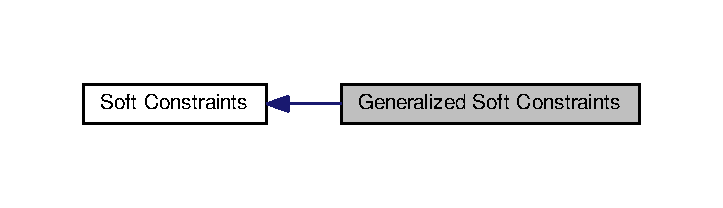
\includegraphics[width=347pt]{group__generalized__sc}
\end{center}
\end{figure}
\subsection*{Macros}
\begin{DoxyCompactItemize}
\item 
\hypertarget{group__generalized__sc_ga8bd41ebc8039378d242e4e8c273716a5}{\#define \hyperlink{group__generalized__sc_ga8bd41ebc8039378d242e4e8c273716a5}{V\+R\+N\+A\+\_\+\+D\+E\+C\+O\+M\+P\+\_\+\+P\+A\+I\+R\+\_\+\+H\+P}~1}\label{group__generalized__sc_ga8bd41ebc8039378d242e4e8c273716a5}

\begin{DoxyCompactList}\small\item\em Generalized constraint folding flag indicating hairpin loop decomposition step. \end{DoxyCompactList}\item 
\hypertarget{group__generalized__sc_gaeab04f34d7730cff2d651d782f95d857}{\#define \hyperlink{group__generalized__sc_gaeab04f34d7730cff2d651d782f95d857}{V\+R\+N\+A\+\_\+\+D\+E\+C\+O\+M\+P\+\_\+\+P\+A\+I\+R\+\_\+\+I\+L}~2}\label{group__generalized__sc_gaeab04f34d7730cff2d651d782f95d857}

\begin{DoxyCompactList}\small\item\em Generalized constraint folding flag indicating interior loop decomposition step. \end{DoxyCompactList}\end{DoxyCompactItemize}
\subsection*{Typedefs}
\begin{DoxyCompactItemize}
\item 
typedef int( \hyperlink{group__generalized__sc_ga2f3d2d2333e5a616e0f5cd4823780c0c}{vrna\+\_\+callback\+\_\+sc\+\_\+energy} )(int i, int j, int k, int l, char d, void $\ast$data)
\begin{DoxyCompactList}\small\item\em Callback to retrieve pseudo energy contribution for soft constraint feature. \end{DoxyCompactList}\item 
typedef \hyperlink{group__data__structures_ga31125aeace516926bf7f251f759b6126}{F\+L\+T\+\_\+\+O\+R\+\_\+\+D\+B\+L}( \hyperlink{group__generalized__sc_ga28d5138cc47eb7a5116c87518fd076a9}{vrna\+\_\+callback\+\_\+sc\+\_\+exp\+\_\+energy} )(int i, int j, int k, int l, char d, void $\ast$data)
\begin{DoxyCompactList}\small\item\em Callback to retrieve pseudo energy contribution as Boltzmann Factors for soft constraint feature. \end{DoxyCompactList}\item 
typedef \hyperlink{group__data__structures_gac8c5669d3fb813cacf506489689305ce}{vrna\+\_\+basepair\+\_\+t} $\ast$( \hyperlink{group__generalized__sc_ga1157aec50aa078464b868b5d2245ebf5}{vrna\+\_\+callback\+\_\+sc\+\_\+backtrack} )(int i, int j, int k, int l, char d, void $\ast$data)
\begin{DoxyCompactList}\small\item\em Callback to retrieve auxiliary base pairs for soft constraint feature. \end{DoxyCompactList}\end{DoxyCompactItemize}
\subsection*{Functions}
\begin{DoxyCompactItemize}
\item 
void \hyperlink{group__generalized__sc_ga8c7d907ec0125cd61c04e0908010a4e9}{vrna\+\_\+sc\+\_\+add\+\_\+f} (\hyperlink{group__fold__compound_ga1b0cef17fd40466cef5968eaeeff6166}{vrna\+\_\+fold\+\_\+compound\+\_\+t} $\ast$vc, \hyperlink{group__generalized__sc_ga2f3d2d2333e5a616e0f5cd4823780c0c}{vrna\+\_\+callback\+\_\+sc\+\_\+energy} $\ast$f)
\begin{DoxyCompactList}\small\item\em Bind a function pointer for generalized soft constraint feature (M\+F\+E version) \end{DoxyCompactList}\item 
void \hyperlink{group__generalized__sc_gabde7d07a79bb9a8f4721aee247b674ea}{vrna\+\_\+sc\+\_\+add\+\_\+bt} (\hyperlink{group__fold__compound_ga1b0cef17fd40466cef5968eaeeff6166}{vrna\+\_\+fold\+\_\+compound\+\_\+t} $\ast$vc, \hyperlink{group__generalized__sc_ga1157aec50aa078464b868b5d2245ebf5}{vrna\+\_\+callback\+\_\+sc\+\_\+backtrack} $\ast$f)
\begin{DoxyCompactList}\small\item\em Bind a backtracking function pointer for generalized soft constraint feature. \end{DoxyCompactList}\item 
void \hyperlink{group__generalized__sc_ga87e382b5d0c9b7d9ce1b79c0473ff700}{vrna\+\_\+sc\+\_\+add\+\_\+exp\+\_\+f} (\hyperlink{group__fold__compound_ga1b0cef17fd40466cef5968eaeeff6166}{vrna\+\_\+fold\+\_\+compound\+\_\+t} $\ast$vc, \hyperlink{group__generalized__sc_ga28d5138cc47eb7a5116c87518fd076a9}{vrna\+\_\+callback\+\_\+sc\+\_\+exp\+\_\+energy} $\ast$exp\+\_\+f)
\begin{DoxyCompactList}\small\item\em Bind a function pointer for generalized soft constraint feature (P\+F version) \end{DoxyCompactList}\end{DoxyCompactItemize}
\begin{DoxyCompactItemize}
\item 
int \hyperlink{group__generalized__sc_gaa6ff0113a3a76dc0b8d62961f4e1dfa0}{vrna\+\_\+sc\+\_\+add\+\_\+hi\+\_\+motif} (\hyperlink{group__fold__compound_ga1b0cef17fd40466cef5968eaeeff6166}{vrna\+\_\+fold\+\_\+compound\+\_\+t} $\ast$vc, const char $\ast$seq, const char $\ast$structure, \hyperlink{group__data__structures_ga31125aeace516926bf7f251f759b6126}{F\+L\+T\+\_\+\+O\+R\+\_\+\+D\+B\+L} energy, unsigned int options)
\begin{DoxyCompactList}\small\item\em Add soft constraints for hairpin or interior loop binding motif. \end{DoxyCompactList}\end{DoxyCompactItemize}


\subsection{Detailed Description}


\subsection{Typedef Documentation}
\hypertarget{group__generalized__sc_ga2f3d2d2333e5a616e0f5cd4823780c0c}{\index{Generalized Soft Constraints@{Generalized Soft Constraints}!vrna\+\_\+callback\+\_\+sc\+\_\+energy@{vrna\+\_\+callback\+\_\+sc\+\_\+energy}}
\index{vrna\+\_\+callback\+\_\+sc\+\_\+energy@{vrna\+\_\+callback\+\_\+sc\+\_\+energy}!Generalized Soft Constraints@{Generalized Soft Constraints}}
\subsubsection[{vrna\+\_\+callback\+\_\+sc\+\_\+energy}]{\setlength{\rightskip}{0pt plus 5cm}typedef int( vrna\+\_\+callback\+\_\+sc\+\_\+energy)(int i, int j, int k, int l, char d, void $\ast$data)}}\label{group__generalized__sc_ga2f3d2d2333e5a616e0f5cd4823780c0c}


{\ttfamily \#include $<$\hyperlink{constraints_8h}{Vienna\+R\+N\+A/constraints.\+h}$>$}



Callback to retrieve pseudo energy contribution for soft constraint feature. 


\begin{DoxyParams}{Parameters}
{\em i} & Left (5') delimiter position of substructure \\
\hline
{\em j} & Right (3') delimiter position of substructure \\
\hline
{\em k} & \\
\hline
{\em l} & \\
\hline
{\em d} & Decomposition step indicator \\
\hline
{\em data} & Auxiliary data \\
\hline
\end{DoxyParams}
\begin{DoxyReturn}{Returns}
Pseudo energy contribution in deka-\/kalories per mol 
\end{DoxyReturn}
\hypertarget{group__generalized__sc_ga28d5138cc47eb7a5116c87518fd076a9}{\index{Generalized Soft Constraints@{Generalized Soft Constraints}!vrna\+\_\+callback\+\_\+sc\+\_\+exp\+\_\+energy@{vrna\+\_\+callback\+\_\+sc\+\_\+exp\+\_\+energy}}
\index{vrna\+\_\+callback\+\_\+sc\+\_\+exp\+\_\+energy@{vrna\+\_\+callback\+\_\+sc\+\_\+exp\+\_\+energy}!Generalized Soft Constraints@{Generalized Soft Constraints}}
\subsubsection[{vrna\+\_\+callback\+\_\+sc\+\_\+exp\+\_\+energy}]{\setlength{\rightskip}{0pt plus 5cm}typedef {\bf F\+L\+T\+\_\+\+O\+R\+\_\+\+D\+B\+L}( vrna\+\_\+callback\+\_\+sc\+\_\+exp\+\_\+energy)(int i, int j, int k, int l, char d, void $\ast$data)}}\label{group__generalized__sc_ga28d5138cc47eb7a5116c87518fd076a9}


{\ttfamily \#include $<$\hyperlink{constraints_8h}{Vienna\+R\+N\+A/constraints.\+h}$>$}



Callback to retrieve pseudo energy contribution as Boltzmann Factors for soft constraint feature. 


\begin{DoxyParams}{Parameters}
{\em i} & Left (5') delimiter position of substructure \\
\hline
{\em j} & Right (3') delimiter position of substructure \\
\hline
{\em k} & \\
\hline
{\em l} & \\
\hline
{\em d} & Decomposition step indicator \\
\hline
{\em data} & Auxiliary data \\
\hline
\end{DoxyParams}
\begin{DoxyReturn}{Returns}
Pseudo energy contribution in deka-\/kalories per mol 
\end{DoxyReturn}
\hypertarget{group__generalized__sc_ga1157aec50aa078464b868b5d2245ebf5}{\index{Generalized Soft Constraints@{Generalized Soft Constraints}!vrna\+\_\+callback\+\_\+sc\+\_\+backtrack@{vrna\+\_\+callback\+\_\+sc\+\_\+backtrack}}
\index{vrna\+\_\+callback\+\_\+sc\+\_\+backtrack@{vrna\+\_\+callback\+\_\+sc\+\_\+backtrack}!Generalized Soft Constraints@{Generalized Soft Constraints}}
\subsubsection[{vrna\+\_\+callback\+\_\+sc\+\_\+backtrack}]{\setlength{\rightskip}{0pt plus 5cm}typedef {\bf vrna\+\_\+basepair\+\_\+t}$\ast$( vrna\+\_\+callback\+\_\+sc\+\_\+backtrack)(int i, int j, int k, int l, char d, void $\ast$data)}}\label{group__generalized__sc_ga1157aec50aa078464b868b5d2245ebf5}


{\ttfamily \#include $<$\hyperlink{constraints_8h}{Vienna\+R\+N\+A/constraints.\+h}$>$}



Callback to retrieve auxiliary base pairs for soft constraint feature. 


\begin{DoxyParams}{Parameters}
{\em i} & Left (5') delimiter position of substructure \\
\hline
{\em j} & Right (3') delimiter position of substructure \\
\hline
{\em k} & \\
\hline
{\em l} & \\
\hline
{\em d} & Decomposition step indicator \\
\hline
{\em data} & Auxiliary data \\
\hline
\end{DoxyParams}
\begin{DoxyReturn}{Returns}
List of additional base pairs 
\end{DoxyReturn}


\subsection{Function Documentation}
\hypertarget{group__generalized__sc_ga8c7d907ec0125cd61c04e0908010a4e9}{\index{Generalized Soft Constraints@{Generalized Soft Constraints}!vrna\+\_\+sc\+\_\+add\+\_\+f@{vrna\+\_\+sc\+\_\+add\+\_\+f}}
\index{vrna\+\_\+sc\+\_\+add\+\_\+f@{vrna\+\_\+sc\+\_\+add\+\_\+f}!Generalized Soft Constraints@{Generalized Soft Constraints}}
\subsubsection[{vrna\+\_\+sc\+\_\+add\+\_\+f}]{\setlength{\rightskip}{0pt plus 5cm}void vrna\+\_\+sc\+\_\+add\+\_\+f (
\begin{DoxyParamCaption}
\item[{{\bf vrna\+\_\+fold\+\_\+compound\+\_\+t} $\ast$}]{vc, }
\item[{{\bf vrna\+\_\+callback\+\_\+sc\+\_\+energy} $\ast$}]{f}
\end{DoxyParamCaption}
)}}\label{group__generalized__sc_ga8c7d907ec0125cd61c04e0908010a4e9}


{\ttfamily \#include $<$\hyperlink{constraints_8h}{Vienna\+R\+N\+A/constraints.\+h}$>$}



Bind a function pointer for generalized soft constraint feature (M\+F\+E version) 

This function allows to easily bind a function pointer and corresponding data structure to the soft constraint part \hyperlink{group__constraints_ga75401ce219ef8dbcceb672db82d434c6}{vrna\+\_\+sc\+\_\+t} of the \hyperlink{group__fold__compound_ga1b0cef17fd40466cef5968eaeeff6166}{vrna\+\_\+fold\+\_\+compound\+\_\+t}. The function for evaluating the generalized soft constraint feature has to return a pseudo free energy $ \hat{E} $ in $ dacal/mol $, where $ 1 dacal/mol = 10 cal/mol $.


\begin{DoxyParams}{Parameters}
{\em vc} & The fold compound the generalized soft constraint function should be bound to \\
\hline
{\em f} & A pointer to the function that evaluates the generalized soft constraint feature \\
\hline
{\em data} & A pointer to the data structure that holds required data for function 'f' \\
\hline
\end{DoxyParams}
\hypertarget{group__generalized__sc_gabde7d07a79bb9a8f4721aee247b674ea}{\index{Generalized Soft Constraints@{Generalized Soft Constraints}!vrna\+\_\+sc\+\_\+add\+\_\+bt@{vrna\+\_\+sc\+\_\+add\+\_\+bt}}
\index{vrna\+\_\+sc\+\_\+add\+\_\+bt@{vrna\+\_\+sc\+\_\+add\+\_\+bt}!Generalized Soft Constraints@{Generalized Soft Constraints}}
\subsubsection[{vrna\+\_\+sc\+\_\+add\+\_\+bt}]{\setlength{\rightskip}{0pt plus 5cm}void vrna\+\_\+sc\+\_\+add\+\_\+bt (
\begin{DoxyParamCaption}
\item[{{\bf vrna\+\_\+fold\+\_\+compound\+\_\+t} $\ast$}]{vc, }
\item[{{\bf vrna\+\_\+callback\+\_\+sc\+\_\+backtrack} $\ast$}]{f}
\end{DoxyParamCaption}
)}}\label{group__generalized__sc_gabde7d07a79bb9a8f4721aee247b674ea}


{\ttfamily \#include $<$\hyperlink{constraints_8h}{Vienna\+R\+N\+A/constraints.\+h}$>$}



Bind a backtracking function pointer for generalized soft constraint feature. 

This function allows to easily bind a function pointer to the soft constraint part \hyperlink{group__constraints_ga75401ce219ef8dbcceb672db82d434c6}{vrna\+\_\+sc\+\_\+t} of the \hyperlink{group__fold__compound_ga1b0cef17fd40466cef5968eaeeff6166}{vrna\+\_\+fold\+\_\+compound\+\_\+t}. The provided function should be used for backtracking purposes in loop regions that were altered via the generalized soft constraint feature. It has to return an array of \hyperlink{group__data__structures_gac8c5669d3fb813cacf506489689305ce}{vrna\+\_\+basepair\+\_\+t} data structures, were the last element in the list is indicated by a value of -\/1 in it's i position.


\begin{DoxyParams}{Parameters}
{\em vc} & The fold compound the generalized soft constraint function should be bound to \\
\hline
{\em f} & A pointer to the function that returns additional base pairs \\
\hline
\end{DoxyParams}
\hypertarget{group__generalized__sc_ga87e382b5d0c9b7d9ce1b79c0473ff700}{\index{Generalized Soft Constraints@{Generalized Soft Constraints}!vrna\+\_\+sc\+\_\+add\+\_\+exp\+\_\+f@{vrna\+\_\+sc\+\_\+add\+\_\+exp\+\_\+f}}
\index{vrna\+\_\+sc\+\_\+add\+\_\+exp\+\_\+f@{vrna\+\_\+sc\+\_\+add\+\_\+exp\+\_\+f}!Generalized Soft Constraints@{Generalized Soft Constraints}}
\subsubsection[{vrna\+\_\+sc\+\_\+add\+\_\+exp\+\_\+f}]{\setlength{\rightskip}{0pt plus 5cm}void vrna\+\_\+sc\+\_\+add\+\_\+exp\+\_\+f (
\begin{DoxyParamCaption}
\item[{{\bf vrna\+\_\+fold\+\_\+compound\+\_\+t} $\ast$}]{vc, }
\item[{{\bf vrna\+\_\+callback\+\_\+sc\+\_\+exp\+\_\+energy} $\ast$}]{exp\+\_\+f}
\end{DoxyParamCaption}
)}}\label{group__generalized__sc_ga87e382b5d0c9b7d9ce1b79c0473ff700}


{\ttfamily \#include $<$\hyperlink{constraints_8h}{Vienna\+R\+N\+A/constraints.\+h}$>$}



Bind a function pointer for generalized soft constraint feature (P\+F version) 

This function allows to easily bind a function pointer and corresponding data structure to the soft constraint part \hyperlink{group__constraints_ga75401ce219ef8dbcceb672db82d434c6}{vrna\+\_\+sc\+\_\+t} of the \hyperlink{group__fold__compound_ga1b0cef17fd40466cef5968eaeeff6166}{vrna\+\_\+fold\+\_\+compound\+\_\+t}. The function for evaluating the generalized soft constraint feature has to return a pseudo free energy $ \hat{E} $ as Boltzmann factor, i.\+e. $ exp(- \hat{E} / kT) $. The required unit for $ E $ is $ cal/mol $.


\begin{DoxyParams}{Parameters}
{\em vc} & The fold compound the generalized soft constraint function should be bound to \\
\hline
{\em exp\+\_\+f} & A pointer to the function that evaluates the generalized soft constraint feature \\
\hline
{\em data} & A pointer to the data structure that holds required data for function 'f' \\
\hline
\end{DoxyParams}
\hypertarget{group__generalized__sc_gaa6ff0113a3a76dc0b8d62961f4e1dfa0}{\index{Generalized Soft Constraints@{Generalized Soft Constraints}!vrna\+\_\+sc\+\_\+add\+\_\+hi\+\_\+motif@{vrna\+\_\+sc\+\_\+add\+\_\+hi\+\_\+motif}}
\index{vrna\+\_\+sc\+\_\+add\+\_\+hi\+\_\+motif@{vrna\+\_\+sc\+\_\+add\+\_\+hi\+\_\+motif}!Generalized Soft Constraints@{Generalized Soft Constraints}}
\subsubsection[{vrna\+\_\+sc\+\_\+add\+\_\+hi\+\_\+motif}]{\setlength{\rightskip}{0pt plus 5cm}int vrna\+\_\+sc\+\_\+add\+\_\+hi\+\_\+motif (
\begin{DoxyParamCaption}
\item[{{\bf vrna\+\_\+fold\+\_\+compound\+\_\+t} $\ast$}]{vc, }
\item[{const char $\ast$}]{seq, }
\item[{const char $\ast$}]{structure, }
\item[{{\bf F\+L\+T\+\_\+\+O\+R\+\_\+\+D\+B\+L}}]{energy, }
\item[{unsigned int}]{options}
\end{DoxyParamCaption}
)}}\label{group__generalized__sc_gaa6ff0113a3a76dc0b8d62961f4e1dfa0}


{\ttfamily \#include $<$\hyperlink{ligand_8h}{Vienna\+R\+N\+A/ligand.\+h}$>$}



Add soft constraints for hairpin or interior loop binding motif. 

Here is an example that adds a theophylline binding motif. Free energy contribution is derived from $k_d = 0.32 \mu mol / l $, taken from Jenison et al. 1994 
\begin{DoxyCode}
\hyperlink{group__generalized__sc_gaa6ff0113a3a76dc0b8d62961f4e1dfa0}{vrna\_sc\_add\_hi\_motif}( vc,
                      \textcolor{stringliteral}{"GAUACCAG&CCCUUGGCAGC"},
                      \textcolor{stringliteral}{"(...((((&)...)))...)"},
                      -9.22,
                      \hyperlink{group__fold__compound_gae63be9127fe7dcc1f9bb14f5bb1064ee}{VRNA\_OPTION\_MFE}); 
\end{DoxyCode}



\begin{DoxyParams}{Parameters}
{\em vc} & The \hyperlink{group__fold__compound_ga1b0cef17fd40466cef5968eaeeff6166}{vrna\+\_\+fold\+\_\+compound\+\_\+t} the motif is applied to \\
\hline
{\em seq} & The sequence motif (may be interspaced by '\&' character \\
\hline
{\em structure} & The structure motif (may be interspaced by '\&' character \\
\hline
{\em energy} & The free energy of the motif (e.\+g. binding free energy) \\
\hline
{\em options} & Options indicating whether to use the motif in M\+F\+E prediction, and/or P\+F predictions \\
\hline
\end{DoxyParams}
\begin{DoxyReturn}{Returns}
non-\/zero value if application of the motif using soft constraints was successful 
\end{DoxyReturn}

\include{group__fold__compound}
\hypertarget{group__dp__matrices}{}\section{The Dynamic Programming Matrices}
\label{group__dp__matrices}\index{The Dynamic Programming Matrices@{The Dynamic Programming Matrices}}


This module provides interfaces that deal with creation and destruction of dynamic programming matrices used within the R\+N\+Alib.  


Collaboration diagram for The Dynamic Programming Matrices\+:
\nopagebreak
\begin{figure}[H]
\begin{center}
\leavevmode
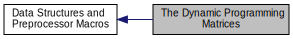
\includegraphics[width=350pt]{group__dp__matrices}
\end{center}
\end{figure}
\subsection*{Data Structures}
\begin{DoxyCompactItemize}
\item 
struct \hyperlink{group__dp__matrices_structvrna__mx__mfe__s}{vrna\+\_\+mx\+\_\+mfe\+\_\+s}
\begin{DoxyCompactList}\small\item\em Minimum Free Energy (M\+F\+E) Dynamic Programming (D\+P) matrices data structure required within the \hyperlink{group__fold__compound_ga1b0cef17fd40466cef5968eaeeff6166}{vrna\+\_\+fold\+\_\+compound\+\_\+t}.  \hyperlink{group__dp__matrices_structvrna__mx__mfe__s}{More...}\end{DoxyCompactList}\item 
struct \hyperlink{group__dp__matrices_structvrna__mx__pf__s}{vrna\+\_\+mx\+\_\+pf\+\_\+s}
\begin{DoxyCompactList}\small\item\em Partition function (P\+F) Dynamic Programming (D\+P) matrices data structure required within the \hyperlink{group__fold__compound_ga1b0cef17fd40466cef5968eaeeff6166}{vrna\+\_\+fold\+\_\+compound\+\_\+t}.  \hyperlink{group__dp__matrices_structvrna__mx__pf__s}{More...}\end{DoxyCompactList}\end{DoxyCompactItemize}
\subsection*{Typedefs}
\begin{DoxyCompactItemize}
\item 
\hypertarget{group__dp__matrices_gae5aef35d016475e758f619b7bcb534f9}{}typedef struct \hyperlink{group__dp__matrices_structvrna__mx__mfe__s}{vrna\+\_\+mx\+\_\+mfe\+\_\+s} \hyperlink{group__dp__matrices_gae5aef35d016475e758f619b7bcb534f9}{vrna\+\_\+mx\+\_\+mfe\+\_\+t}\label{group__dp__matrices_gae5aef35d016475e758f619b7bcb534f9}

\begin{DoxyCompactList}\small\item\em Typename for the Minimum Free Energy (M\+F\+E) D\+P matrices data structure \hyperlink{group__dp__matrices_structvrna__mx__mfe__s}{vrna\+\_\+mx\+\_\+mfe\+\_\+s}. \end{DoxyCompactList}\item 
\hypertarget{group__dp__matrices_ga68729ab3fed26bdd1806fa814f172fc1}{}typedef struct \hyperlink{group__dp__matrices_structvrna__mx__pf__s}{vrna\+\_\+mx\+\_\+pf\+\_\+s} \hyperlink{group__dp__matrices_ga68729ab3fed26bdd1806fa814f172fc1}{vrna\+\_\+mx\+\_\+pf\+\_\+t}\label{group__dp__matrices_ga68729ab3fed26bdd1806fa814f172fc1}

\begin{DoxyCompactList}\small\item\em Typename for the Partition Function (P\+F) D\+P matrices data structure \hyperlink{group__dp__matrices_structvrna__mx__pf__s}{vrna\+\_\+mx\+\_\+pf\+\_\+s}. \end{DoxyCompactList}\end{DoxyCompactItemize}
\subsection*{Enumerations}
\begin{DoxyCompactItemize}
\item 
enum \hyperlink{group__dp__matrices_ga6042ea1d58d01931e959791be6d89343}{vrna\+\_\+mx\+\_\+type\+\_\+e} \{ \hyperlink{group__dp__matrices_gga6042ea1d58d01931e959791be6d89343aafa2568956dab79595521e20c49a5f75}{V\+R\+N\+A\+\_\+\+M\+X\+\_\+\+D\+E\+F\+A\+U\+L\+T}, 
\hyperlink{group__dp__matrices_gga6042ea1d58d01931e959791be6d89343a2ea5d5947f6ec02544934b0ff2785e99}{V\+R\+N\+A\+\_\+\+M\+X\+\_\+\+W\+I\+N\+D\+O\+W}, 
\hyperlink{group__dp__matrices_gga6042ea1d58d01931e959791be6d89343ae656f8391445ff71bed8a597a0a19417}{V\+R\+N\+A\+\_\+\+M\+X\+\_\+2\+D\+F\+O\+L\+D}
 \}
\begin{DoxyCompactList}\small\item\em An enumerator that is used to specify the type of a polymorphic Dynamic Programming (D\+P) matrix data structure. \end{DoxyCompactList}\end{DoxyCompactItemize}
\subsection*{Functions}
\begin{DoxyCompactItemize}
\item 
int \hyperlink{group__dp__matrices_ga08661f098008961dab0023bf300f0c33}{vrna\+\_\+mx\+\_\+add} (\hyperlink{group__fold__compound_ga1b0cef17fd40466cef5968eaeeff6166}{vrna\+\_\+fold\+\_\+compound\+\_\+t} $\ast$vc, \hyperlink{group__dp__matrices_ga6042ea1d58d01931e959791be6d89343}{vrna\+\_\+mx\+\_\+type\+\_\+e} type, unsigned int options)
\begin{DoxyCompactList}\small\item\em Add Dynamic Programming (D\+P) matrices (allocate memory) \end{DoxyCompactList}\item 
void \hyperlink{group__dp__matrices_ga6a9422feb5dfe5c64050cebf447672d0}{vrna\+\_\+mx\+\_\+mfe\+\_\+free} (\hyperlink{group__fold__compound_ga1b0cef17fd40466cef5968eaeeff6166}{vrna\+\_\+fold\+\_\+compound\+\_\+t} $\ast$vc)
\begin{DoxyCompactList}\small\item\em Free memory occupied by the Minimum Free Energy (M\+F\+E) Dynamic Programming (D\+P) matrices. \end{DoxyCompactList}\item 
void \hyperlink{group__dp__matrices_ga2283e69fd139fb8e58d7ade3b5773f9c}{vrna\+\_\+mx\+\_\+pf\+\_\+free} (\hyperlink{group__fold__compound_ga1b0cef17fd40466cef5968eaeeff6166}{vrna\+\_\+fold\+\_\+compound\+\_\+t} $\ast$vc)
\begin{DoxyCompactList}\small\item\em Free memory occupied by the Partition Function (P\+F) Dynamic Programming (D\+P) matrices. \end{DoxyCompactList}\end{DoxyCompactItemize}


\subsection{Detailed Description}
This module provides interfaces that deal with creation and destruction of dynamic programming matrices used within the R\+N\+Alib. 



\subsection{Data Structure Documentation}
\index{vrna\+\_\+mx\+\_\+mfe\+\_\+s@{vrna\+\_\+mx\+\_\+mfe\+\_\+s}}\label{structvrna__mx__mfe__s}
\hypertarget{group__dp__matrices_structvrna__mx__mfe__s}{}
\subsubsection{struct vrna\+\_\+mx\+\_\+mfe\+\_\+s}
Minimum Free Energy (M\+F\+E) Dynamic Programming (D\+P) matrices data structure required within the \hyperlink{group__fold__compound_ga1b0cef17fd40466cef5968eaeeff6166}{vrna\+\_\+fold\+\_\+compound\+\_\+t}. \subsubsection*{Data Fields}
\begin{Indent}{\bf Common fields for M\+F\+E matrices}\par
\begin{DoxyCompactItemize}
\item 
\hypertarget{group__dp__matrices_a468680aa937b664d453075108d976ae2}{}\hyperlink{group__dp__matrices_ga6042ea1d58d01931e959791be6d89343}{vrna\+\_\+mx\+\_\+type\+\_\+e} {\bfseries type}\label{group__dp__matrices_a468680aa937b664d453075108d976ae2}

\item 
\hypertarget{group__dp__matrices_a1f92a8406fc1fb721dbf9193c34ad826}{}unsigned int \hyperlink{group__dp__matrices_a1f92a8406fc1fb721dbf9193c34ad826}{length}\label{group__dp__matrices_a1f92a8406fc1fb721dbf9193c34ad826}

\begin{DoxyCompactList}\small\item\em Length of the sequence, therefore an indicator of the size of the D\+P matrices. \end{DoxyCompactList}\end{DoxyCompactItemize}
\end{Indent}
\begin{Indent}{\bf Default D\+P matrices}\par
{\em \begin{DoxyNote}{Note}
These data fields are available if 
\begin{DoxyCode}
\hyperlink{group__dp__matrices_structvrna__mx__mfe__s}{vrna\_mx\_mfe\_t}.type == \hyperlink{group__dp__matrices_gga6042ea1d58d01931e959791be6d89343aafa2568956dab79595521e20c49a5f75}{VRNA\_MX\_DEFAULT} 
\end{DoxyCode}
 
\end{DoxyNote}
}\begin{DoxyCompactItemize}
\item 
\hypertarget{group__dp__matrices_a60a511fd42905ee4f046c56a76865bf9}{}int $\ast$ \hyperlink{group__dp__matrices_a60a511fd42905ee4f046c56a76865bf9}{c}\label{group__dp__matrices_a60a511fd42905ee4f046c56a76865bf9}

\begin{DoxyCompactList}\small\item\em Energy array, given that i-\/j pair. \end{DoxyCompactList}\item 
\hypertarget{group__dp__matrices_abebad693be987c2701d64477ab858039}{}int $\ast$ \hyperlink{group__dp__matrices_abebad693be987c2701d64477ab858039}{f5}\label{group__dp__matrices_abebad693be987c2701d64477ab858039}

\begin{DoxyCompactList}\small\item\em Energy of 5\textquotesingle{} end. \end{DoxyCompactList}\item 
\hypertarget{group__dp__matrices_a4ea4595a93733adef047ece8e6f5da52}{}int $\ast$ \hyperlink{group__dp__matrices_a4ea4595a93733adef047ece8e6f5da52}{f3}\label{group__dp__matrices_a4ea4595a93733adef047ece8e6f5da52}

\begin{DoxyCompactList}\small\item\em Energy of 3\textquotesingle{} end. \end{DoxyCompactList}\item 
\hypertarget{group__dp__matrices_a8ee6b6cefe20cfbf1f6bef5c788b6667}{}int $\ast$ \hyperlink{group__dp__matrices_a8ee6b6cefe20cfbf1f6bef5c788b6667}{fc}\label{group__dp__matrices_a8ee6b6cefe20cfbf1f6bef5c788b6667}

\begin{DoxyCompactList}\small\item\em Energy from i to cutpoint (and vice versa if i$>$cut) \end{DoxyCompactList}\item 
\hypertarget{group__dp__matrices_a103995e4ab8e21e7f8bc36a6edcb1331}{}int $\ast$ \hyperlink{group__dp__matrices_a103995e4ab8e21e7f8bc36a6edcb1331}{f\+M\+L}\label{group__dp__matrices_a103995e4ab8e21e7f8bc36a6edcb1331}

\begin{DoxyCompactList}\small\item\em Multi-\/loop auxiliary energy array. \end{DoxyCompactList}\item 
\hypertarget{group__dp__matrices_ae4e598d601f5ece6b8b4ffffcae2db06}{}int $\ast$ \hyperlink{group__dp__matrices_ae4e598d601f5ece6b8b4ffffcae2db06}{f\+M1}\label{group__dp__matrices_ae4e598d601f5ece6b8b4ffffcae2db06}

\begin{DoxyCompactList}\small\item\em Second M\+L array, only for unique multibrnach loop decomposition. \end{DoxyCompactList}\item 
\hypertarget{group__dp__matrices_ad29106e37d485b3f20b7be468e6c179c}{}int $\ast$ \hyperlink{group__dp__matrices_ad29106e37d485b3f20b7be468e6c179c}{f\+M2}\label{group__dp__matrices_ad29106e37d485b3f20b7be468e6c179c}

\begin{DoxyCompactList}\small\item\em Energy for a multibranch loop region with exactly two stems, extending to 3\textquotesingle{} end. \end{DoxyCompactList}\item 
\hypertarget{group__dp__matrices_a0b7b86a5c75c96eabb89eb53a13e7164}{}int $\ast$ \hyperlink{group__dp__matrices_a0b7b86a5c75c96eabb89eb53a13e7164}{ggg}\label{group__dp__matrices_a0b7b86a5c75c96eabb89eb53a13e7164}

\begin{DoxyCompactList}\small\item\em Energies of g-\/quadruplexes. \end{DoxyCompactList}\item 
\hypertarget{group__dp__matrices_ac6a22d71c6a0eccedf978372b19b458a}{}int \hyperlink{group__dp__matrices_ac6a22d71c6a0eccedf978372b19b458a}{Fc}\label{group__dp__matrices_ac6a22d71c6a0eccedf978372b19b458a}

\begin{DoxyCompactList}\small\item\em Minimum Free Energy of entire circular R\+N\+A. \end{DoxyCompactList}\item 
\hypertarget{group__dp__matrices_a1ba03c53ee2a32eaf8b46c0eb259e0c4}{}int {\bfseries Fc\+H}\label{group__dp__matrices_a1ba03c53ee2a32eaf8b46c0eb259e0c4}

\item 
\hypertarget{group__dp__matrices_a96ac173770c9745a30823fa17fe0b7f4}{}int {\bfseries Fc\+I}\label{group__dp__matrices_a96ac173770c9745a30823fa17fe0b7f4}

\item 
\hypertarget{group__dp__matrices_a9a4bf70926f79372388eccc7e73759e9}{}int {\bfseries Fc\+M}\label{group__dp__matrices_a9a4bf70926f79372388eccc7e73759e9}

\end{DoxyCompactItemize}
\end{Indent}
\begin{Indent}{\bf Local Folding D\+P matrices using window approach}\par
{\em \begin{DoxyNote}{Note}
These data fields are available if 
\begin{DoxyCode}
\hyperlink{group__dp__matrices_structvrna__mx__mfe__s}{vrna\_mx\_mfe\_t}.type == \hyperlink{group__dp__matrices_gga6042ea1d58d01931e959791be6d89343a2ea5d5947f6ec02544934b0ff2785e99}{VRNA\_MX\_WINDOW} 
\end{DoxyCode}
 
\end{DoxyNote}
}\begin{DoxyCompactItemize}
\item 
\hypertarget{group__dp__matrices_a116c677ece0832e6ab9cc2fd1ebfe452}{}int $\ast$$\ast$ \hyperlink{group__dp__matrices_a116c677ece0832e6ab9cc2fd1ebfe452}{c\+\_\+local}\label{group__dp__matrices_a116c677ece0832e6ab9cc2fd1ebfe452}

\begin{DoxyCompactList}\small\item\em Energy array, given that i-\/j pair. \end{DoxyCompactList}\item 
\hypertarget{group__dp__matrices_a6eae0a2b696b0c63bbaa78a70b950600}{}int $\ast$ \hyperlink{group__dp__matrices_a6eae0a2b696b0c63bbaa78a70b950600}{f3\+\_\+local}\label{group__dp__matrices_a6eae0a2b696b0c63bbaa78a70b950600}

\begin{DoxyCompactList}\small\item\em Energy of 5\textquotesingle{} end. \end{DoxyCompactList}\item 
\hypertarget{group__dp__matrices_ad37d705240a8e6b1e9a4e4ea19e74003}{}int $\ast$$\ast$ \hyperlink{group__dp__matrices_ad37d705240a8e6b1e9a4e4ea19e74003}{f\+M\+L\+\_\+local}\label{group__dp__matrices_ad37d705240a8e6b1e9a4e4ea19e74003}

\begin{DoxyCompactList}\small\item\em Multi-\/loop auxiliary energy array. \end{DoxyCompactList}\item 
\hypertarget{group__dp__matrices_afd3ea65bc8f06559f7f1ea79072fa385}{}int $\ast$$\ast$ \hyperlink{group__dp__matrices_afd3ea65bc8f06559f7f1ea79072fa385}{ggg\+\_\+local}\label{group__dp__matrices_afd3ea65bc8f06559f7f1ea79072fa385}

\begin{DoxyCompactList}\small\item\em Energies of g-\/quadruplexes. \end{DoxyCompactList}\end{DoxyCompactItemize}
\end{Indent}
\begin{Indent}{\bf Distance Class D\+P matrices}\par
{\em \begin{DoxyNote}{Note}
These data fields are available if 
\begin{DoxyCode}
\hyperlink{group__dp__matrices_structvrna__mx__mfe__s}{vrna\_mx\_mfe\_t}.type == \hyperlink{group__dp__matrices_gga6042ea1d58d01931e959791be6d89343ae656f8391445ff71bed8a597a0a19417}{VRNA\_MX\_2DFOLD} 
\end{DoxyCode}
 
\end{DoxyNote}
}\begin{DoxyCompactItemize}
\item 
\hypertarget{group__dp__matrices_ab917aa1e2b069af7fb5d11c5d067cdf0}{}int $\ast$$\ast$$\ast$ {\bfseries E\+\_\+\+F5}\label{group__dp__matrices_ab917aa1e2b069af7fb5d11c5d067cdf0}

\item 
\hypertarget{group__dp__matrices_a4035d3c6a9e23e388ddec18a9fdc2315}{}int $\ast$$\ast$ {\bfseries l\+\_\+min\+\_\+\+F5}\label{group__dp__matrices_a4035d3c6a9e23e388ddec18a9fdc2315}

\item 
\hypertarget{group__dp__matrices_a794ba42ca5afa5320a2da88554928516}{}int $\ast$$\ast$ {\bfseries l\+\_\+max\+\_\+\+F5}\label{group__dp__matrices_a794ba42ca5afa5320a2da88554928516}

\item 
\hypertarget{group__dp__matrices_aad6fc641a5815149b8d938ca277019a5}{}int $\ast$ {\bfseries k\+\_\+min\+\_\+\+F5}\label{group__dp__matrices_aad6fc641a5815149b8d938ca277019a5}

\item 
\hypertarget{group__dp__matrices_a321a00180a1d046796328d0a9b66ec81}{}int $\ast$ {\bfseries k\+\_\+max\+\_\+\+F5}\label{group__dp__matrices_a321a00180a1d046796328d0a9b66ec81}

\item 
\hypertarget{group__dp__matrices_a4d055707928eb6f3147c962141cc70e8}{}int $\ast$$\ast$$\ast$ {\bfseries E\+\_\+\+F3}\label{group__dp__matrices_a4d055707928eb6f3147c962141cc70e8}

\item 
\hypertarget{group__dp__matrices_abf0389ece58e97652f580d7dc1e133d8}{}int $\ast$$\ast$ {\bfseries l\+\_\+min\+\_\+\+F3}\label{group__dp__matrices_abf0389ece58e97652f580d7dc1e133d8}

\item 
\hypertarget{group__dp__matrices_afadce4435141575c7275b1e0b75e8eba}{}int $\ast$$\ast$ {\bfseries l\+\_\+max\+\_\+\+F3}\label{group__dp__matrices_afadce4435141575c7275b1e0b75e8eba}

\item 
\hypertarget{group__dp__matrices_a063fb9477172048bd24786ef363315db}{}int $\ast$ {\bfseries k\+\_\+min\+\_\+\+F3}\label{group__dp__matrices_a063fb9477172048bd24786ef363315db}

\item 
\hypertarget{group__dp__matrices_a1e20cd5b9d422f547b3366e74b59b1bd}{}int $\ast$ {\bfseries k\+\_\+max\+\_\+\+F3}\label{group__dp__matrices_a1e20cd5b9d422f547b3366e74b59b1bd}

\item 
\hypertarget{group__dp__matrices_af7007bfa68981a0d7a7a2186c357eb4f}{}int $\ast$$\ast$$\ast$ {\bfseries E\+\_\+\+C}\label{group__dp__matrices_af7007bfa68981a0d7a7a2186c357eb4f}

\item 
\hypertarget{group__dp__matrices_a33f9c476304c568c78918a5bcc3e2c2f}{}int $\ast$$\ast$ {\bfseries l\+\_\+min\+\_\+\+C}\label{group__dp__matrices_a33f9c476304c568c78918a5bcc3e2c2f}

\item 
\hypertarget{group__dp__matrices_afb0db136ff9fd3c78ad30816aa276ed3}{}int $\ast$$\ast$ {\bfseries l\+\_\+max\+\_\+\+C}\label{group__dp__matrices_afb0db136ff9fd3c78ad30816aa276ed3}

\item 
\hypertarget{group__dp__matrices_a37d2df63ba2ae973059279f325b0e617}{}int $\ast$ {\bfseries k\+\_\+min\+\_\+\+C}\label{group__dp__matrices_a37d2df63ba2ae973059279f325b0e617}

\item 
\hypertarget{group__dp__matrices_a9bb98ec849469ab7dda8042384a0114e}{}int $\ast$ {\bfseries k\+\_\+max\+\_\+\+C}\label{group__dp__matrices_a9bb98ec849469ab7dda8042384a0114e}

\item 
\hypertarget{group__dp__matrices_aace1bc1fb8f3e0e83296a91e40bda7a5}{}int $\ast$$\ast$$\ast$ {\bfseries E\+\_\+\+M}\label{group__dp__matrices_aace1bc1fb8f3e0e83296a91e40bda7a5}

\item 
\hypertarget{group__dp__matrices_a48afd9784e58e427fcbe4694d4670c57}{}int $\ast$$\ast$ {\bfseries l\+\_\+min\+\_\+\+M}\label{group__dp__matrices_a48afd9784e58e427fcbe4694d4670c57}

\item 
\hypertarget{group__dp__matrices_a59641489689bf8ba2236466b4a9be82a}{}int $\ast$$\ast$ {\bfseries l\+\_\+max\+\_\+\+M}\label{group__dp__matrices_a59641489689bf8ba2236466b4a9be82a}

\item 
\hypertarget{group__dp__matrices_a7a723bdda23a431fa498b6e46f71de05}{}int $\ast$ {\bfseries k\+\_\+min\+\_\+\+M}\label{group__dp__matrices_a7a723bdda23a431fa498b6e46f71de05}

\item 
\hypertarget{group__dp__matrices_a45f8584d5a51e734de9376889e9a890e}{}int $\ast$ {\bfseries k\+\_\+max\+\_\+\+M}\label{group__dp__matrices_a45f8584d5a51e734de9376889e9a890e}

\item 
\hypertarget{group__dp__matrices_a2a0eccd64e94962e9ec7c0652c5adcf2}{}int $\ast$$\ast$$\ast$ {\bfseries E\+\_\+\+M1}\label{group__dp__matrices_a2a0eccd64e94962e9ec7c0652c5adcf2}

\item 
\hypertarget{group__dp__matrices_a83ceae2cd2fa2a478fbc917419f4f43c}{}int $\ast$$\ast$ {\bfseries l\+\_\+min\+\_\+\+M1}\label{group__dp__matrices_a83ceae2cd2fa2a478fbc917419f4f43c}

\item 
\hypertarget{group__dp__matrices_abacc2eb5bd2798188191693d562941fe}{}int $\ast$$\ast$ {\bfseries l\+\_\+max\+\_\+\+M1}\label{group__dp__matrices_abacc2eb5bd2798188191693d562941fe}

\item 
\hypertarget{group__dp__matrices_a31b0f5d774d868d3723b0e98a64ab4c2}{}int $\ast$ {\bfseries k\+\_\+min\+\_\+\+M1}\label{group__dp__matrices_a31b0f5d774d868d3723b0e98a64ab4c2}

\item 
\hypertarget{group__dp__matrices_ad7aa8ad7e4246927b79f0e69cfdb20b2}{}int $\ast$ {\bfseries k\+\_\+max\+\_\+\+M1}\label{group__dp__matrices_ad7aa8ad7e4246927b79f0e69cfdb20b2}

\item 
\hypertarget{group__dp__matrices_a84f072a7e5a9d1dc978e92b3a78f53f8}{}int $\ast$$\ast$$\ast$ {\bfseries E\+\_\+\+M2}\label{group__dp__matrices_a84f072a7e5a9d1dc978e92b3a78f53f8}

\item 
\hypertarget{group__dp__matrices_a0ee034810d6ece4cd0f4604ec4c94c22}{}int $\ast$$\ast$ {\bfseries l\+\_\+min\+\_\+\+M2}\label{group__dp__matrices_a0ee034810d6ece4cd0f4604ec4c94c22}

\item 
\hypertarget{group__dp__matrices_a0d78bbbc4621247d97f00160803a05b0}{}int $\ast$$\ast$ {\bfseries l\+\_\+max\+\_\+\+M2}\label{group__dp__matrices_a0d78bbbc4621247d97f00160803a05b0}

\item 
\hypertarget{group__dp__matrices_a27eede8de57b179fc24839bc25e96be0}{}int $\ast$ {\bfseries k\+\_\+min\+\_\+\+M2}\label{group__dp__matrices_a27eede8de57b179fc24839bc25e96be0}

\item 
\hypertarget{group__dp__matrices_ac3bc074f2b291247b65d34e336ef064f}{}int $\ast$ {\bfseries k\+\_\+max\+\_\+\+M2}\label{group__dp__matrices_ac3bc074f2b291247b65d34e336ef064f}

\item 
\hypertarget{group__dp__matrices_ac81b8edd7d1297b43af1c163214ec95b}{}int $\ast$$\ast$ {\bfseries E\+\_\+\+Fc}\label{group__dp__matrices_ac81b8edd7d1297b43af1c163214ec95b}

\item 
\hypertarget{group__dp__matrices_a64f1fdc523370d4d27f4e74db37ec3f2}{}int $\ast$ {\bfseries l\+\_\+min\+\_\+\+Fc}\label{group__dp__matrices_a64f1fdc523370d4d27f4e74db37ec3f2}

\item 
\hypertarget{group__dp__matrices_a253b64237c811ef8587de8a714658365}{}int $\ast$ {\bfseries l\+\_\+max\+\_\+\+Fc}\label{group__dp__matrices_a253b64237c811ef8587de8a714658365}

\item 
\hypertarget{group__dp__matrices_a3b381c1a816112c9557056a52db5d104}{}int {\bfseries k\+\_\+min\+\_\+\+Fc}\label{group__dp__matrices_a3b381c1a816112c9557056a52db5d104}

\item 
\hypertarget{group__dp__matrices_a2aa2123340602899bd7a61d82db95a3f}{}int {\bfseries k\+\_\+max\+\_\+\+Fc}\label{group__dp__matrices_a2aa2123340602899bd7a61d82db95a3f}

\item 
\hypertarget{group__dp__matrices_a366499237acdae5e4f422e4bc82bfc0d}{}int $\ast$$\ast$ {\bfseries E\+\_\+\+Fc\+H}\label{group__dp__matrices_a366499237acdae5e4f422e4bc82bfc0d}

\item 
\hypertarget{group__dp__matrices_a5d0a6a5cd45a42d23fc0eabf0763caa8}{}int $\ast$ {\bfseries l\+\_\+min\+\_\+\+Fc\+H}\label{group__dp__matrices_a5d0a6a5cd45a42d23fc0eabf0763caa8}

\item 
\hypertarget{group__dp__matrices_a89192a2ab2c8de9f5b702edc9fe68613}{}int $\ast$ {\bfseries l\+\_\+max\+\_\+\+Fc\+H}\label{group__dp__matrices_a89192a2ab2c8de9f5b702edc9fe68613}

\item 
\hypertarget{group__dp__matrices_aa3f7198e3c6207737934088d27639911}{}int {\bfseries k\+\_\+min\+\_\+\+Fc\+H}\label{group__dp__matrices_aa3f7198e3c6207737934088d27639911}

\item 
\hypertarget{group__dp__matrices_a8e94d63c103c7effce55652619b3b469}{}int {\bfseries k\+\_\+max\+\_\+\+Fc\+H}\label{group__dp__matrices_a8e94d63c103c7effce55652619b3b469}

\item 
\hypertarget{group__dp__matrices_a3e9793de5245f038ed83c2a607b37970}{}int $\ast$$\ast$ {\bfseries E\+\_\+\+Fc\+I}\label{group__dp__matrices_a3e9793de5245f038ed83c2a607b37970}

\item 
\hypertarget{group__dp__matrices_abc4dd9942f140f91adb52d2719e78bc4}{}int $\ast$ {\bfseries l\+\_\+min\+\_\+\+Fc\+I}\label{group__dp__matrices_abc4dd9942f140f91adb52d2719e78bc4}

\item 
\hypertarget{group__dp__matrices_a41cb6dbbda30f5d7bafd6b0ea62bca8c}{}int $\ast$ {\bfseries l\+\_\+max\+\_\+\+Fc\+I}\label{group__dp__matrices_a41cb6dbbda30f5d7bafd6b0ea62bca8c}

\item 
\hypertarget{group__dp__matrices_acbf5d0bd27435ad5328482f9b4b32833}{}int {\bfseries k\+\_\+min\+\_\+\+Fc\+I}\label{group__dp__matrices_acbf5d0bd27435ad5328482f9b4b32833}

\item 
\hypertarget{group__dp__matrices_a6b13abef4bee7a08fd28b0780535373e}{}int {\bfseries k\+\_\+max\+\_\+\+Fc\+I}\label{group__dp__matrices_a6b13abef4bee7a08fd28b0780535373e}

\item 
\hypertarget{group__dp__matrices_aad18f800b7bc0f26d012b9bc36aa5382}{}int $\ast$$\ast$ {\bfseries E\+\_\+\+Fc\+M}\label{group__dp__matrices_aad18f800b7bc0f26d012b9bc36aa5382}

\item 
\hypertarget{group__dp__matrices_a7ee24b747cf1d4ecc1cdc7380cf39594}{}int $\ast$ {\bfseries l\+\_\+min\+\_\+\+Fc\+M}\label{group__dp__matrices_a7ee24b747cf1d4ecc1cdc7380cf39594}

\item 
\hypertarget{group__dp__matrices_a0d419ae5a7e10b98734d42f5391d25f5}{}int $\ast$ {\bfseries l\+\_\+max\+\_\+\+Fc\+M}\label{group__dp__matrices_a0d419ae5a7e10b98734d42f5391d25f5}

\item 
\hypertarget{group__dp__matrices_a36089cee4d38f465f79db7e3589693a7}{}int {\bfseries k\+\_\+min\+\_\+\+Fc\+M}\label{group__dp__matrices_a36089cee4d38f465f79db7e3589693a7}

\item 
\hypertarget{group__dp__matrices_aa5a4d2fd78e38c82ee666f9bdc911e66}{}int {\bfseries k\+\_\+max\+\_\+\+Fc\+M}\label{group__dp__matrices_aa5a4d2fd78e38c82ee666f9bdc911e66}

\item 
\hypertarget{group__dp__matrices_af286d9ea990a98a33c065b4e16eaa311}{}int $\ast$ {\bfseries E\+\_\+\+F5\+\_\+rem}\label{group__dp__matrices_af286d9ea990a98a33c065b4e16eaa311}

\item 
\hypertarget{group__dp__matrices_afa8e42da47467e098bab0c6f1c16bea4}{}int $\ast$ {\bfseries E\+\_\+\+F3\+\_\+rem}\label{group__dp__matrices_afa8e42da47467e098bab0c6f1c16bea4}

\item 
\hypertarget{group__dp__matrices_a00f20c8bd9eda2ebcd99267cce52909c}{}int $\ast$ {\bfseries E\+\_\+\+C\+\_\+rem}\label{group__dp__matrices_a00f20c8bd9eda2ebcd99267cce52909c}

\item 
\hypertarget{group__dp__matrices_a92b0234e1e3cdaba2dea416e37904a09}{}int $\ast$ {\bfseries E\+\_\+\+M\+\_\+rem}\label{group__dp__matrices_a92b0234e1e3cdaba2dea416e37904a09}

\item 
\hypertarget{group__dp__matrices_a89dddd61f360292fddcc9b25e7cbc699}{}int $\ast$ {\bfseries E\+\_\+\+M1\+\_\+rem}\label{group__dp__matrices_a89dddd61f360292fddcc9b25e7cbc699}

\item 
\hypertarget{group__dp__matrices_a5fc042fba42b3676226b64fb4ab80ad2}{}int $\ast$ {\bfseries E\+\_\+\+M2\+\_\+rem}\label{group__dp__matrices_a5fc042fba42b3676226b64fb4ab80ad2}

\item 
\hypertarget{group__dp__matrices_aec03a4d7538bfa0e1113ba2825175428}{}int {\bfseries E\+\_\+\+Fc\+\_\+rem}\label{group__dp__matrices_aec03a4d7538bfa0e1113ba2825175428}

\item 
\hypertarget{group__dp__matrices_a120dc87d9b5f452b12ab796046a0f704}{}int {\bfseries E\+\_\+\+Fc\+H\+\_\+rem}\label{group__dp__matrices_a120dc87d9b5f452b12ab796046a0f704}

\item 
\hypertarget{group__dp__matrices_add53b23599a083140d0ddbd158a84d1d}{}int {\bfseries E\+\_\+\+Fc\+I\+\_\+rem}\label{group__dp__matrices_add53b23599a083140d0ddbd158a84d1d}

\item 
\hypertarget{group__dp__matrices_ad821cb861e772e1c0fd4efddb44380c7}{}int {\bfseries E\+\_\+\+Fc\+M\+\_\+rem}\label{group__dp__matrices_ad821cb861e772e1c0fd4efddb44380c7}

\end{DoxyCompactItemize}
\end{Indent}
\index{vrna\+\_\+mx\+\_\+pf\+\_\+s@{vrna\+\_\+mx\+\_\+pf\+\_\+s}}\label{structvrna__mx__pf__s}
\hypertarget{group__dp__matrices_structvrna__mx__pf__s}{}
\subsubsection{struct vrna\+\_\+mx\+\_\+pf\+\_\+s}
Partition function (P\+F) Dynamic Programming (D\+P) matrices data structure required within the \hyperlink{group__fold__compound_ga1b0cef17fd40466cef5968eaeeff6166}{vrna\+\_\+fold\+\_\+compound\+\_\+t}. \subsubsection*{Data Fields}
\begin{Indent}{\bf Common fields for D\+P matrices}\par
\begin{DoxyCompactItemize}
\item 
\hypertarget{group__dp__matrices_a74ba745d6fc4ac5d437bc24450ea789c}{}\hyperlink{group__dp__matrices_ga6042ea1d58d01931e959791be6d89343}{vrna\+\_\+mx\+\_\+type\+\_\+e} {\bfseries type}\label{group__dp__matrices_a74ba745d6fc4ac5d437bc24450ea789c}

\item 
\hypertarget{group__dp__matrices_a798f72ece3f3f970bb0de2120600ad63}{}unsigned int {\bfseries length}\label{group__dp__matrices_a798f72ece3f3f970bb0de2120600ad63}

\item 
\hypertarget{group__dp__matrices_a133ac57938cb0969da254a594572baf8}{}\hyperlink{group__data__structures_ga31125aeace516926bf7f251f759b6126}{F\+L\+T\+\_\+\+O\+R\+\_\+\+D\+B\+L} $\ast$ {\bfseries scale}\label{group__dp__matrices_a133ac57938cb0969da254a594572baf8}

\item 
\hypertarget{group__dp__matrices_ae18e83833416f62943d5dd7be1cc038f}{}\hyperlink{group__data__structures_ga31125aeace516926bf7f251f759b6126}{F\+L\+T\+\_\+\+O\+R\+\_\+\+D\+B\+L} $\ast$ {\bfseries exp\+M\+Lbase}\label{group__dp__matrices_ae18e83833416f62943d5dd7be1cc038f}

\end{DoxyCompactItemize}
\end{Indent}
\begin{Indent}{\bf Default P\+F matrices}\par
{\em \begin{DoxyNote}{Note}
These data fields are available if 
\begin{DoxyCode}
\hyperlink{group__dp__matrices_structvrna__mx__pf__s}{vrna\_mx\_pf\_t}.type == \hyperlink{group__dp__matrices_gga6042ea1d58d01931e959791be6d89343aafa2568956dab79595521e20c49a5f75}{VRNA\_MX\_DEFAULT} 
\end{DoxyCode}
 
\end{DoxyNote}
}\begin{DoxyCompactItemize}
\item 
\hypertarget{group__dp__matrices_a033a0277ac33736256c6a13f13d75879}{}\hyperlink{group__data__structures_ga31125aeace516926bf7f251f759b6126}{F\+L\+T\+\_\+\+O\+R\+\_\+\+D\+B\+L} $\ast$ {\bfseries q}\label{group__dp__matrices_a033a0277ac33736256c6a13f13d75879}

\item 
\hypertarget{group__dp__matrices_abd5ea8aa63458625d0c8b2a868fcfa28}{}\hyperlink{group__data__structures_ga31125aeace516926bf7f251f759b6126}{F\+L\+T\+\_\+\+O\+R\+\_\+\+D\+B\+L} $\ast$ {\bfseries qb}\label{group__dp__matrices_abd5ea8aa63458625d0c8b2a868fcfa28}

\item 
\hypertarget{group__dp__matrices_a612e774309a7fd0b6812200aa31f87d5}{}\hyperlink{group__data__structures_ga31125aeace516926bf7f251f759b6126}{F\+L\+T\+\_\+\+O\+R\+\_\+\+D\+B\+L} $\ast$ {\bfseries qm}\label{group__dp__matrices_a612e774309a7fd0b6812200aa31f87d5}

\item 
\hypertarget{group__dp__matrices_ad60e1fd6fa490ae72cdd899c37a52165}{}\hyperlink{group__data__structures_ga31125aeace516926bf7f251f759b6126}{F\+L\+T\+\_\+\+O\+R\+\_\+\+D\+B\+L} $\ast$ {\bfseries qm1}\label{group__dp__matrices_ad60e1fd6fa490ae72cdd899c37a52165}

\item 
\hypertarget{group__dp__matrices_aee4b900811aa012ab135838e2e5868f2}{}\hyperlink{group__data__structures_ga31125aeace516926bf7f251f759b6126}{F\+L\+T\+\_\+\+O\+R\+\_\+\+D\+B\+L} $\ast$ {\bfseries probs}\label{group__dp__matrices_aee4b900811aa012ab135838e2e5868f2}

\item 
\hypertarget{group__dp__matrices_a6ee76a2c5cefd1a9d6addf0a32071124}{}\hyperlink{group__data__structures_ga31125aeace516926bf7f251f759b6126}{F\+L\+T\+\_\+\+O\+R\+\_\+\+D\+B\+L} $\ast$ {\bfseries q1k}\label{group__dp__matrices_a6ee76a2c5cefd1a9d6addf0a32071124}

\item 
\hypertarget{group__dp__matrices_ae3a10b81e574b966d062e705b4ad8168}{}\hyperlink{group__data__structures_ga31125aeace516926bf7f251f759b6126}{F\+L\+T\+\_\+\+O\+R\+\_\+\+D\+B\+L} $\ast$ {\bfseries qln}\label{group__dp__matrices_ae3a10b81e574b966d062e705b4ad8168}

\item 
\hypertarget{group__dp__matrices_a40d61ddad03db0ba06e1848ce9004138}{}\hyperlink{group__data__structures_ga31125aeace516926bf7f251f759b6126}{F\+L\+T\+\_\+\+O\+R\+\_\+\+D\+B\+L} $\ast$ {\bfseries G}\label{group__dp__matrices_a40d61ddad03db0ba06e1848ce9004138}

\item 
\hypertarget{group__dp__matrices_a160e39f74bfcd3f94c77bdf334070782}{}\hyperlink{group__data__structures_ga31125aeace516926bf7f251f759b6126}{F\+L\+T\+\_\+\+O\+R\+\_\+\+D\+B\+L} {\bfseries qo}\label{group__dp__matrices_a160e39f74bfcd3f94c77bdf334070782}

\item 
\hypertarget{group__dp__matrices_a0a4ff1fd1b71810ccab242a862cfdf8c}{}\hyperlink{group__data__structures_ga31125aeace516926bf7f251f759b6126}{F\+L\+T\+\_\+\+O\+R\+\_\+\+D\+B\+L} $\ast$ {\bfseries qm2}\label{group__dp__matrices_a0a4ff1fd1b71810ccab242a862cfdf8c}

\item 
\hypertarget{group__dp__matrices_a0841b18e38c22bb92df7efee9caaabb0}{}\hyperlink{group__data__structures_ga31125aeace516926bf7f251f759b6126}{F\+L\+T\+\_\+\+O\+R\+\_\+\+D\+B\+L} {\bfseries qho}\label{group__dp__matrices_a0841b18e38c22bb92df7efee9caaabb0}

\item 
\hypertarget{group__dp__matrices_ac9c23d0dd3a0bb150c389399afe119eb}{}\hyperlink{group__data__structures_ga31125aeace516926bf7f251f759b6126}{F\+L\+T\+\_\+\+O\+R\+\_\+\+D\+B\+L} {\bfseries qio}\label{group__dp__matrices_ac9c23d0dd3a0bb150c389399afe119eb}

\item 
\hypertarget{group__dp__matrices_a970e8f6dfdf874185a9d4f77a942f61c}{}\hyperlink{group__data__structures_ga31125aeace516926bf7f251f759b6126}{F\+L\+T\+\_\+\+O\+R\+\_\+\+D\+B\+L} {\bfseries qmo}\label{group__dp__matrices_a970e8f6dfdf874185a9d4f77a942f61c}

\end{DoxyCompactItemize}
\end{Indent}
\begin{Indent}{\bf Distance Class D\+P matrices}\par
{\em \begin{DoxyNote}{Note}
These data fields are available if 
\begin{DoxyCode}
\hyperlink{group__dp__matrices_structvrna__mx__pf__s}{vrna\_mx\_pf\_t}.type == \hyperlink{group__dp__matrices_gga6042ea1d58d01931e959791be6d89343ae656f8391445ff71bed8a597a0a19417}{VRNA\_MX\_2DFOLD} 
\end{DoxyCode}
 
\end{DoxyNote}
}\begin{DoxyCompactItemize}
\item 
\hypertarget{group__dp__matrices_a29678f1d17a805ce2c80d765e00f694d}{}\hyperlink{group__data__structures_ga31125aeace516926bf7f251f759b6126}{F\+L\+T\+\_\+\+O\+R\+\_\+\+D\+B\+L} $\ast$$\ast$$\ast$ {\bfseries Q}\label{group__dp__matrices_a29678f1d17a805ce2c80d765e00f694d}

\item 
\hypertarget{group__dp__matrices_a13ccc584739950bcd6de23925a9afe0e}{}int $\ast$$\ast$ {\bfseries l\+\_\+min\+\_\+\+Q}\label{group__dp__matrices_a13ccc584739950bcd6de23925a9afe0e}

\item 
\hypertarget{group__dp__matrices_ac136ef6871aad05b013aaec2a4cc9298}{}int $\ast$$\ast$ {\bfseries l\+\_\+max\+\_\+\+Q}\label{group__dp__matrices_ac136ef6871aad05b013aaec2a4cc9298}

\item 
\hypertarget{group__dp__matrices_aa09c7b59d39b4b669173330976ae4798}{}int $\ast$ {\bfseries k\+\_\+min\+\_\+\+Q}\label{group__dp__matrices_aa09c7b59d39b4b669173330976ae4798}

\item 
\hypertarget{group__dp__matrices_a6405e58faa7aac0d7fd7bf6fc2821b99}{}int $\ast$ {\bfseries k\+\_\+max\+\_\+\+Q}\label{group__dp__matrices_a6405e58faa7aac0d7fd7bf6fc2821b99}

\item 
\hypertarget{group__dp__matrices_a7bf41bf6ce96a6a6ffad912a6bb9f023}{}\hyperlink{group__data__structures_ga31125aeace516926bf7f251f759b6126}{F\+L\+T\+\_\+\+O\+R\+\_\+\+D\+B\+L} $\ast$$\ast$$\ast$ {\bfseries Q\+\_\+\+B}\label{group__dp__matrices_a7bf41bf6ce96a6a6ffad912a6bb9f023}

\item 
\hypertarget{group__dp__matrices_aa6ab6ade9a4f4aa347ea1ac3d780bbf4}{}int $\ast$$\ast$ {\bfseries l\+\_\+min\+\_\+\+Q\+\_\+\+B}\label{group__dp__matrices_aa6ab6ade9a4f4aa347ea1ac3d780bbf4}

\item 
\hypertarget{group__dp__matrices_a7a6b46c40f038de8798e009ead7e5c81}{}int $\ast$$\ast$ {\bfseries l\+\_\+max\+\_\+\+Q\+\_\+\+B}\label{group__dp__matrices_a7a6b46c40f038de8798e009ead7e5c81}

\item 
\hypertarget{group__dp__matrices_a32a61364685e55e2cb90c3bef635fe9e}{}int $\ast$ {\bfseries k\+\_\+min\+\_\+\+Q\+\_\+\+B}\label{group__dp__matrices_a32a61364685e55e2cb90c3bef635fe9e}

\item 
\hypertarget{group__dp__matrices_a4bb8b8fc4b39dbf163584164575253e4}{}int $\ast$ {\bfseries k\+\_\+max\+\_\+\+Q\+\_\+\+B}\label{group__dp__matrices_a4bb8b8fc4b39dbf163584164575253e4}

\item 
\hypertarget{group__dp__matrices_a283eb582a89f62cf7d12bb6afc774ba7}{}\hyperlink{group__data__structures_ga31125aeace516926bf7f251f759b6126}{F\+L\+T\+\_\+\+O\+R\+\_\+\+D\+B\+L} $\ast$$\ast$$\ast$ {\bfseries Q\+\_\+\+M}\label{group__dp__matrices_a283eb582a89f62cf7d12bb6afc774ba7}

\item 
\hypertarget{group__dp__matrices_acdb695807092c9fa8ba32b4c033881b2}{}int $\ast$$\ast$ {\bfseries l\+\_\+min\+\_\+\+Q\+\_\+\+M}\label{group__dp__matrices_acdb695807092c9fa8ba32b4c033881b2}

\item 
\hypertarget{group__dp__matrices_a0e46adc65e479d671aed00097b8f162a}{}int $\ast$$\ast$ {\bfseries l\+\_\+max\+\_\+\+Q\+\_\+\+M}\label{group__dp__matrices_a0e46adc65e479d671aed00097b8f162a}

\item 
\hypertarget{group__dp__matrices_ab3375971ac859512a745d6eec99244d2}{}int $\ast$ {\bfseries k\+\_\+min\+\_\+\+Q\+\_\+\+M}\label{group__dp__matrices_ab3375971ac859512a745d6eec99244d2}

\item 
\hypertarget{group__dp__matrices_a9b9d2a9a7a25929605437af8fe3e7f47}{}int $\ast$ {\bfseries k\+\_\+max\+\_\+\+Q\+\_\+\+M}\label{group__dp__matrices_a9b9d2a9a7a25929605437af8fe3e7f47}

\item 
\hypertarget{group__dp__matrices_a3ebab8245e0d6747c8cb4068fcb2f14c}{}\hyperlink{group__data__structures_ga31125aeace516926bf7f251f759b6126}{F\+L\+T\+\_\+\+O\+R\+\_\+\+D\+B\+L} $\ast$$\ast$$\ast$ {\bfseries Q\+\_\+\+M1}\label{group__dp__matrices_a3ebab8245e0d6747c8cb4068fcb2f14c}

\item 
\hypertarget{group__dp__matrices_a798dd2cc60f5af4b93dac4cba0459683}{}int $\ast$$\ast$ {\bfseries l\+\_\+min\+\_\+\+Q\+\_\+\+M1}\label{group__dp__matrices_a798dd2cc60f5af4b93dac4cba0459683}

\item 
\hypertarget{group__dp__matrices_afec22c55d9cdea707596702ce40221ec}{}int $\ast$$\ast$ {\bfseries l\+\_\+max\+\_\+\+Q\+\_\+\+M1}\label{group__dp__matrices_afec22c55d9cdea707596702ce40221ec}

\item 
\hypertarget{group__dp__matrices_a89548e61d9fbf7936f9e46aed2296813}{}int $\ast$ {\bfseries k\+\_\+min\+\_\+\+Q\+\_\+\+M1}\label{group__dp__matrices_a89548e61d9fbf7936f9e46aed2296813}

\item 
\hypertarget{group__dp__matrices_abb96656ec2020302fb1e1c9394ff2519}{}int $\ast$ {\bfseries k\+\_\+max\+\_\+\+Q\+\_\+\+M1}\label{group__dp__matrices_abb96656ec2020302fb1e1c9394ff2519}

\item 
\hypertarget{group__dp__matrices_a4271859f583cc0b27d0bfb6951c050f5}{}\hyperlink{group__data__structures_ga31125aeace516926bf7f251f759b6126}{F\+L\+T\+\_\+\+O\+R\+\_\+\+D\+B\+L} $\ast$$\ast$$\ast$ {\bfseries Q\+\_\+\+M2}\label{group__dp__matrices_a4271859f583cc0b27d0bfb6951c050f5}

\item 
\hypertarget{group__dp__matrices_ad23a0e61af82fdf8243c10000d418a8f}{}int $\ast$$\ast$ {\bfseries l\+\_\+min\+\_\+\+Q\+\_\+\+M2}\label{group__dp__matrices_ad23a0e61af82fdf8243c10000d418a8f}

\item 
\hypertarget{group__dp__matrices_a8182f4fd762fcb853a78ae818e275114}{}int $\ast$$\ast$ {\bfseries l\+\_\+max\+\_\+\+Q\+\_\+\+M2}\label{group__dp__matrices_a8182f4fd762fcb853a78ae818e275114}

\item 
\hypertarget{group__dp__matrices_ac76826db329f701f0abf43d9e1a4446c}{}int $\ast$ {\bfseries k\+\_\+min\+\_\+\+Q\+\_\+\+M2}\label{group__dp__matrices_ac76826db329f701f0abf43d9e1a4446c}

\item 
\hypertarget{group__dp__matrices_a9dc7897463d929ff56198e3cd79aa531}{}int $\ast$ {\bfseries k\+\_\+max\+\_\+\+Q\+\_\+\+M2}\label{group__dp__matrices_a9dc7897463d929ff56198e3cd79aa531}

\item 
\hypertarget{group__dp__matrices_a50d4c30dd0d535cd3a00c29e2b77c81e}{}\hyperlink{group__data__structures_ga31125aeace516926bf7f251f759b6126}{F\+L\+T\+\_\+\+O\+R\+\_\+\+D\+B\+L} $\ast$$\ast$ {\bfseries Q\+\_\+c}\label{group__dp__matrices_a50d4c30dd0d535cd3a00c29e2b77c81e}

\item 
\hypertarget{group__dp__matrices_a1a165b9e68b552abd6970e7b79398e68}{}int $\ast$ {\bfseries l\+\_\+min\+\_\+\+Q\+\_\+c}\label{group__dp__matrices_a1a165b9e68b552abd6970e7b79398e68}

\item 
\hypertarget{group__dp__matrices_ad16c8bacc50d9ad75fc4d3aad18b3c74}{}int $\ast$ {\bfseries l\+\_\+max\+\_\+\+Q\+\_\+c}\label{group__dp__matrices_ad16c8bacc50d9ad75fc4d3aad18b3c74}

\item 
\hypertarget{group__dp__matrices_aca9ff00550c75057c3f0796526eaa3fd}{}int {\bfseries k\+\_\+min\+\_\+\+Q\+\_\+c}\label{group__dp__matrices_aca9ff00550c75057c3f0796526eaa3fd}

\item 
\hypertarget{group__dp__matrices_ac5cdf53876b9ea8060b7c0fc12b2bdca}{}int {\bfseries k\+\_\+max\+\_\+\+Q\+\_\+c}\label{group__dp__matrices_ac5cdf53876b9ea8060b7c0fc12b2bdca}

\item 
\hypertarget{group__dp__matrices_aba4db9bf16cbe37199838b8ed1ba096c}{}\hyperlink{group__data__structures_ga31125aeace516926bf7f251f759b6126}{F\+L\+T\+\_\+\+O\+R\+\_\+\+D\+B\+L} $\ast$$\ast$ {\bfseries Q\+\_\+c\+H}\label{group__dp__matrices_aba4db9bf16cbe37199838b8ed1ba096c}

\item 
\hypertarget{group__dp__matrices_a08f5bfd11886731ebb3a9f0ba97a0b6b}{}int $\ast$ {\bfseries l\+\_\+min\+\_\+\+Q\+\_\+c\+H}\label{group__dp__matrices_a08f5bfd11886731ebb3a9f0ba97a0b6b}

\item 
\hypertarget{group__dp__matrices_a1ac1d79977932e1b7131b47948b3915a}{}int $\ast$ {\bfseries l\+\_\+max\+\_\+\+Q\+\_\+c\+H}\label{group__dp__matrices_a1ac1d79977932e1b7131b47948b3915a}

\item 
\hypertarget{group__dp__matrices_a763eab70c62986a630fd0013d1931ea8}{}int {\bfseries k\+\_\+min\+\_\+\+Q\+\_\+c\+H}\label{group__dp__matrices_a763eab70c62986a630fd0013d1931ea8}

\item 
\hypertarget{group__dp__matrices_a8093a0a48f24c26e575b18e5d59b1e5c}{}int {\bfseries k\+\_\+max\+\_\+\+Q\+\_\+c\+H}\label{group__dp__matrices_a8093a0a48f24c26e575b18e5d59b1e5c}

\item 
\hypertarget{group__dp__matrices_a1db737927aabceddad13832191c5fa27}{}\hyperlink{group__data__structures_ga31125aeace516926bf7f251f759b6126}{F\+L\+T\+\_\+\+O\+R\+\_\+\+D\+B\+L} $\ast$$\ast$ {\bfseries Q\+\_\+c\+I}\label{group__dp__matrices_a1db737927aabceddad13832191c5fa27}

\item 
\hypertarget{group__dp__matrices_a9e0b38f8272badd75df592524e383973}{}int $\ast$ {\bfseries l\+\_\+min\+\_\+\+Q\+\_\+c\+I}\label{group__dp__matrices_a9e0b38f8272badd75df592524e383973}

\item 
\hypertarget{group__dp__matrices_a852c2d9450a188cc49d72150f7647e48}{}int $\ast$ {\bfseries l\+\_\+max\+\_\+\+Q\+\_\+c\+I}\label{group__dp__matrices_a852c2d9450a188cc49d72150f7647e48}

\item 
\hypertarget{group__dp__matrices_addf9d5e7d009a936651fa1b98421e2bd}{}int {\bfseries k\+\_\+min\+\_\+\+Q\+\_\+c\+I}\label{group__dp__matrices_addf9d5e7d009a936651fa1b98421e2bd}

\item 
\hypertarget{group__dp__matrices_abc3dd1b2bf0f90647e8c73c93432b154}{}int {\bfseries k\+\_\+max\+\_\+\+Q\+\_\+c\+I}\label{group__dp__matrices_abc3dd1b2bf0f90647e8c73c93432b154}

\item 
\hypertarget{group__dp__matrices_ae8e6bc3de40ebe54c7c36677cdc38df8}{}\hyperlink{group__data__structures_ga31125aeace516926bf7f251f759b6126}{F\+L\+T\+\_\+\+O\+R\+\_\+\+D\+B\+L} $\ast$$\ast$ {\bfseries Q\+\_\+c\+M}\label{group__dp__matrices_ae8e6bc3de40ebe54c7c36677cdc38df8}

\item 
\hypertarget{group__dp__matrices_aef4bfb509acba7441d9ace1e0a7e4b93}{}int $\ast$ {\bfseries l\+\_\+min\+\_\+\+Q\+\_\+c\+M}\label{group__dp__matrices_aef4bfb509acba7441d9ace1e0a7e4b93}

\item 
\hypertarget{group__dp__matrices_a57c50e60f1679e2d1add5b48d67b4ad4}{}int $\ast$ {\bfseries l\+\_\+max\+\_\+\+Q\+\_\+c\+M}\label{group__dp__matrices_a57c50e60f1679e2d1add5b48d67b4ad4}

\item 
\hypertarget{group__dp__matrices_ab014ff37700866fd2be6139b3ec470c6}{}int {\bfseries k\+\_\+min\+\_\+\+Q\+\_\+c\+M}\label{group__dp__matrices_ab014ff37700866fd2be6139b3ec470c6}

\item 
\hypertarget{group__dp__matrices_a10c73fd5be9a9bbd350f929d758ac8cf}{}int {\bfseries k\+\_\+max\+\_\+\+Q\+\_\+c\+M}\label{group__dp__matrices_a10c73fd5be9a9bbd350f929d758ac8cf}

\item 
\hypertarget{group__dp__matrices_a9d0f5ad230b36b3553ddf7585c1ae2ec}{}\hyperlink{group__data__structures_ga31125aeace516926bf7f251f759b6126}{F\+L\+T\+\_\+\+O\+R\+\_\+\+D\+B\+L} $\ast$ {\bfseries Q\+\_\+rem}\label{group__dp__matrices_a9d0f5ad230b36b3553ddf7585c1ae2ec}

\item 
\hypertarget{group__dp__matrices_a3e398f1778086b00deb05a3990d533ab}{}\hyperlink{group__data__structures_ga31125aeace516926bf7f251f759b6126}{F\+L\+T\+\_\+\+O\+R\+\_\+\+D\+B\+L} $\ast$ {\bfseries Q\+\_\+\+B\+\_\+rem}\label{group__dp__matrices_a3e398f1778086b00deb05a3990d533ab}

\item 
\hypertarget{group__dp__matrices_a07d9c31f3205d96e094104971b8a85a6}{}\hyperlink{group__data__structures_ga31125aeace516926bf7f251f759b6126}{F\+L\+T\+\_\+\+O\+R\+\_\+\+D\+B\+L} $\ast$ {\bfseries Q\+\_\+\+M\+\_\+rem}\label{group__dp__matrices_a07d9c31f3205d96e094104971b8a85a6}

\item 
\hypertarget{group__dp__matrices_a7d77708c602e982af5a6c1f340d329f4}{}\hyperlink{group__data__structures_ga31125aeace516926bf7f251f759b6126}{F\+L\+T\+\_\+\+O\+R\+\_\+\+D\+B\+L} $\ast$ {\bfseries Q\+\_\+\+M1\+\_\+rem}\label{group__dp__matrices_a7d77708c602e982af5a6c1f340d329f4}

\item 
\hypertarget{group__dp__matrices_a6480ac40d5405af825dee74e3518d6ae}{}\hyperlink{group__data__structures_ga31125aeace516926bf7f251f759b6126}{F\+L\+T\+\_\+\+O\+R\+\_\+\+D\+B\+L} $\ast$ {\bfseries Q\+\_\+\+M2\+\_\+rem}\label{group__dp__matrices_a6480ac40d5405af825dee74e3518d6ae}

\item 
\hypertarget{group__dp__matrices_a0ce7f4b73a6df939f79dfd2f21de80b8}{}\hyperlink{group__data__structures_ga31125aeace516926bf7f251f759b6126}{F\+L\+T\+\_\+\+O\+R\+\_\+\+D\+B\+L} {\bfseries Q\+\_\+c\+\_\+rem}\label{group__dp__matrices_a0ce7f4b73a6df939f79dfd2f21de80b8}

\item 
\hypertarget{group__dp__matrices_aff841b24d39a4f162ba1d10e5109cbe3}{}\hyperlink{group__data__structures_ga31125aeace516926bf7f251f759b6126}{F\+L\+T\+\_\+\+O\+R\+\_\+\+D\+B\+L} {\bfseries Q\+\_\+c\+H\+\_\+rem}\label{group__dp__matrices_aff841b24d39a4f162ba1d10e5109cbe3}

\item 
\hypertarget{group__dp__matrices_a844916b65f091b27e89547f7a51a2dea}{}\hyperlink{group__data__structures_ga31125aeace516926bf7f251f759b6126}{F\+L\+T\+\_\+\+O\+R\+\_\+\+D\+B\+L} {\bfseries Q\+\_\+c\+I\+\_\+rem}\label{group__dp__matrices_a844916b65f091b27e89547f7a51a2dea}

\item 
\hypertarget{group__dp__matrices_a6f6bad095f31114e990d68af46d2eda5}{}\hyperlink{group__data__structures_ga31125aeace516926bf7f251f759b6126}{F\+L\+T\+\_\+\+O\+R\+\_\+\+D\+B\+L} {\bfseries Q\+\_\+c\+M\+\_\+rem}\label{group__dp__matrices_a6f6bad095f31114e990d68af46d2eda5}

\end{DoxyCompactItemize}
\end{Indent}


\subsection{Enumeration Type Documentation}
\hypertarget{group__dp__matrices_ga6042ea1d58d01931e959791be6d89343}{}\index{The Dynamic Programming Matrices@{The Dynamic Programming Matrices}!vrna\+\_\+mx\+\_\+type\+\_\+e@{vrna\+\_\+mx\+\_\+type\+\_\+e}}
\index{vrna\+\_\+mx\+\_\+type\+\_\+e@{vrna\+\_\+mx\+\_\+type\+\_\+e}!The Dynamic Programming Matrices@{The Dynamic Programming Matrices}}
\subsubsection[{vrna\+\_\+mx\+\_\+type\+\_\+e}]{\setlength{\rightskip}{0pt plus 5cm}enum {\bf vrna\+\_\+mx\+\_\+type\+\_\+e}}\label{group__dp__matrices_ga6042ea1d58d01931e959791be6d89343}


{\ttfamily \#include $<$\hyperlink{dp__matrices_8h}{Vienna\+R\+N\+A/dp\+\_\+matrices.\+h}$>$}



An enumerator that is used to specify the type of a polymorphic Dynamic Programming (D\+P) matrix data structure. 

\begin{DoxySeeAlso}{See also}
\hyperlink{group__dp__matrices_gae5aef35d016475e758f619b7bcb534f9}{vrna\+\_\+mx\+\_\+mfe\+\_\+t}, \hyperlink{group__dp__matrices_ga68729ab3fed26bdd1806fa814f172fc1}{vrna\+\_\+mx\+\_\+pf\+\_\+t} 
\end{DoxySeeAlso}
\begin{Desc}
\item[Enumerator]\par
\begin{description}
\index{V\+R\+N\+A\+\_\+\+M\+X\+\_\+\+D\+E\+F\+A\+U\+L\+T@{V\+R\+N\+A\+\_\+\+M\+X\+\_\+\+D\+E\+F\+A\+U\+L\+T}!The Dynamic Programming Matrices@{The Dynamic Programming Matrices}}\index{The Dynamic Programming Matrices@{The Dynamic Programming Matrices}!V\+R\+N\+A\+\_\+\+M\+X\+\_\+\+D\+E\+F\+A\+U\+L\+T@{V\+R\+N\+A\+\_\+\+M\+X\+\_\+\+D\+E\+F\+A\+U\+L\+T}}\item[{\em 
\hypertarget{group__dp__matrices_gga6042ea1d58d01931e959791be6d89343aafa2568956dab79595521e20c49a5f75}{}V\+R\+N\+A\+\_\+\+M\+X\+\_\+\+D\+E\+F\+A\+U\+L\+T\label{group__dp__matrices_gga6042ea1d58d01931e959791be6d89343aafa2568956dab79595521e20c49a5f75}
}]Default D\+P matrices. \index{V\+R\+N\+A\+\_\+\+M\+X\+\_\+\+W\+I\+N\+D\+O\+W@{V\+R\+N\+A\+\_\+\+M\+X\+\_\+\+W\+I\+N\+D\+O\+W}!The Dynamic Programming Matrices@{The Dynamic Programming Matrices}}\index{The Dynamic Programming Matrices@{The Dynamic Programming Matrices}!V\+R\+N\+A\+\_\+\+M\+X\+\_\+\+W\+I\+N\+D\+O\+W@{V\+R\+N\+A\+\_\+\+M\+X\+\_\+\+W\+I\+N\+D\+O\+W}}\item[{\em 
\hypertarget{group__dp__matrices_gga6042ea1d58d01931e959791be6d89343a2ea5d5947f6ec02544934b0ff2785e99}{}V\+R\+N\+A\+\_\+\+M\+X\+\_\+\+W\+I\+N\+D\+O\+W\label{group__dp__matrices_gga6042ea1d58d01931e959791be6d89343a2ea5d5947f6ec02544934b0ff2785e99}
}]D\+P matrices suitable for local structure prediction using window approach. \begin{DoxySeeAlso}{See also}
\hyperlink{group__local__mfe__fold_ga689df235a1915a1ad56e377383c044ce}{vrna\+\_\+mfe\+\_\+window()}, \hyperlink{group__local__mfe__fold_gaa4f67ae94efd08d800c17f9b53423fd6}{vrna\+\_\+mfe\+\_\+window\+\_\+zscore()}, \hyperlink{group__local__pf__fold_ga7dcf599d07258801ea55e7d14a56908d}{pfl\+\_\+fold()} 
\end{DoxySeeAlso}
\index{V\+R\+N\+A\+\_\+\+M\+X\+\_\+2\+D\+F\+O\+L\+D@{V\+R\+N\+A\+\_\+\+M\+X\+\_\+2\+D\+F\+O\+L\+D}!The Dynamic Programming Matrices@{The Dynamic Programming Matrices}}\index{The Dynamic Programming Matrices@{The Dynamic Programming Matrices}!V\+R\+N\+A\+\_\+\+M\+X\+\_\+2\+D\+F\+O\+L\+D@{V\+R\+N\+A\+\_\+\+M\+X\+\_\+2\+D\+F\+O\+L\+D}}\item[{\em 
\hypertarget{group__dp__matrices_gga6042ea1d58d01931e959791be6d89343ae656f8391445ff71bed8a597a0a19417}{}V\+R\+N\+A\+\_\+\+M\+X\+\_\+2\+D\+F\+O\+L\+D\label{group__dp__matrices_gga6042ea1d58d01931e959791be6d89343ae656f8391445ff71bed8a597a0a19417}
}]D\+P matrices suitable for distance class partitioned structure prediction. \begin{DoxySeeAlso}{See also}
\hyperlink{group__kl__neighborhood__mfe_ga243c288b463147352829df04de6a2f77}{vrna\+\_\+mfe\+\_\+\+Two\+D()}, \hyperlink{group__kl__neighborhood__pf_ga0bc3427689bd09da09b8b3094a27f836}{vrna\+\_\+pf\+\_\+\+Two\+D()} 
\end{DoxySeeAlso}
\end{description}
\end{Desc}


\subsection{Function Documentation}
\hypertarget{group__dp__matrices_ga08661f098008961dab0023bf300f0c33}{}\index{The Dynamic Programming Matrices@{The Dynamic Programming Matrices}!vrna\+\_\+mx\+\_\+add@{vrna\+\_\+mx\+\_\+add}}
\index{vrna\+\_\+mx\+\_\+add@{vrna\+\_\+mx\+\_\+add}!The Dynamic Programming Matrices@{The Dynamic Programming Matrices}}
\subsubsection[{vrna\+\_\+mx\+\_\+add}]{\setlength{\rightskip}{0pt plus 5cm}int vrna\+\_\+mx\+\_\+add (
\begin{DoxyParamCaption}
\item[{{\bf vrna\+\_\+fold\+\_\+compound\+\_\+t} $\ast$}]{vc, }
\item[{{\bf vrna\+\_\+mx\+\_\+type\+\_\+e}}]{type, }
\item[{unsigned int}]{options}
\end{DoxyParamCaption}
)}\label{group__dp__matrices_ga08661f098008961dab0023bf300f0c33}


{\ttfamily \#include $<$\hyperlink{dp__matrices_8h}{Vienna\+R\+N\+A/dp\+\_\+matrices.\+h}$>$}



Add Dynamic Programming (D\+P) matrices (allocate memory) 

This function adds D\+P matrices of a specific type to the provided \hyperlink{group__fold__compound_ga1b0cef17fd40466cef5968eaeeff6166}{vrna\+\_\+fold\+\_\+compound\+\_\+t}, such that successive D\+P recursion can be applied. The function caller has to specify which type of D\+P matrix is requested, see \hyperlink{group__dp__matrices_ga6042ea1d58d01931e959791be6d89343}{vrna\+\_\+mx\+\_\+type\+\_\+e}, and what kind of recursive algorithm will be applied later on, using the parameters type, and options, respectively. For the latter, Minimum free energy (M\+F\+E), and Partition function (P\+F) computations are distinguished. A third option that may be passed is \#\+V\+R\+N\+A\+\_\+\+O\+P\+T\+I\+O\+N\+\_\+\+H\+Y\+B\+R\+I\+D, indicating that auxiliary D\+P arrays are required for R\+N\+A-\/\+R\+N\+A interaction prediction.

\begin{DoxyNote}{Note}
Usually, there is no need to call this function, since the constructors of \hyperlink{group__fold__compound_ga1b0cef17fd40466cef5968eaeeff6166}{vrna\+\_\+fold\+\_\+compound\+\_\+t} are handling all the D\+P matrix memory allocation.
\end{DoxyNote}
\begin{DoxySeeAlso}{See also}
vrna\+\_\+mx\+\_\+mfe\+\_\+add(), vrna\+\_\+mx\+\_\+pf\+\_\+add(), \hyperlink{group__fold__compound_ga6601d994ba32b11511b36f68b08403be}{vrna\+\_\+fold\+\_\+compound()}, \hyperlink{group__fold__compound_gad6bacc816af274922b13d947f708aa0c}{vrna\+\_\+fold\+\_\+compound\+\_\+comparative()}, \hyperlink{group__fold__compound_gadded6039d63f5d6509836e20321534ad}{vrna\+\_\+fold\+\_\+compound\+\_\+free()}, \hyperlink{group__dp__matrices_ga2283e69fd139fb8e58d7ade3b5773f9c}{vrna\+\_\+mx\+\_\+pf\+\_\+free()}, \hyperlink{group__dp__matrices_ga6a9422feb5dfe5c64050cebf447672d0}{vrna\+\_\+mx\+\_\+mfe\+\_\+free()}, \hyperlink{group__dp__matrices_ga6042ea1d58d01931e959791be6d89343}{vrna\+\_\+mx\+\_\+type\+\_\+e}, \hyperlink{group__fold__compound_gae63be9127fe7dcc1f9bb14f5bb1064ee}{V\+R\+N\+A\+\_\+\+O\+P\+T\+I\+O\+N\+\_\+\+M\+F\+E}, \hyperlink{group__fold__compound_gabfbadcddda3e74ce7f49035ef8f058f7}{V\+R\+N\+A\+\_\+\+O\+P\+T\+I\+O\+N\+\_\+\+P\+F}, \#\+V\+R\+N\+A\+\_\+\+O\+P\+T\+I\+O\+N\+\_\+\+H\+Y\+B\+R\+I\+D, \hyperlink{group__fold__compound_ga61469c423131552c8483229f8b6c7e0e}{V\+R\+N\+A\+\_\+\+O\+P\+T\+I\+O\+N\+\_\+\+E\+V\+A\+L\+\_\+\+O\+N\+L\+Y}
\end{DoxySeeAlso}

\begin{DoxyParams}{Parameters}
{\em vc} & The \hyperlink{group__fold__compound_ga1b0cef17fd40466cef5968eaeeff6166}{vrna\+\_\+fold\+\_\+compound\+\_\+t} that holds pointers to the D\+P matrices \\
\hline
{\em type} & The type of D\+P matrices requested \\
\hline
{\em options} & Option flags that specify the kind of D\+P matrices, such as M\+F\+E or P\+F arrays, and auxiliary requirements \\
\hline
\end{DoxyParams}
\begin{DoxyReturn}{Returns}
1 if D\+P matrices were properly allocated and attached, 0 otherwise 
\end{DoxyReturn}
\hypertarget{group__dp__matrices_ga6a9422feb5dfe5c64050cebf447672d0}{}\index{The Dynamic Programming Matrices@{The Dynamic Programming Matrices}!vrna\+\_\+mx\+\_\+mfe\+\_\+free@{vrna\+\_\+mx\+\_\+mfe\+\_\+free}}
\index{vrna\+\_\+mx\+\_\+mfe\+\_\+free@{vrna\+\_\+mx\+\_\+mfe\+\_\+free}!The Dynamic Programming Matrices@{The Dynamic Programming Matrices}}
\subsubsection[{vrna\+\_\+mx\+\_\+mfe\+\_\+free}]{\setlength{\rightskip}{0pt plus 5cm}void vrna\+\_\+mx\+\_\+mfe\+\_\+free (
\begin{DoxyParamCaption}
\item[{{\bf vrna\+\_\+fold\+\_\+compound\+\_\+t} $\ast$}]{vc}
\end{DoxyParamCaption}
)}\label{group__dp__matrices_ga6a9422feb5dfe5c64050cebf447672d0}


{\ttfamily \#include $<$\hyperlink{dp__matrices_8h}{Vienna\+R\+N\+A/dp\+\_\+matrices.\+h}$>$}



Free memory occupied by the Minimum Free Energy (M\+F\+E) Dynamic Programming (D\+P) matrices. 

\begin{DoxySeeAlso}{See also}
\hyperlink{group__fold__compound_ga6601d994ba32b11511b36f68b08403be}{vrna\+\_\+fold\+\_\+compound()}, \hyperlink{group__fold__compound_gad6bacc816af274922b13d947f708aa0c}{vrna\+\_\+fold\+\_\+compound\+\_\+comparative()}, \hyperlink{group__fold__compound_gadded6039d63f5d6509836e20321534ad}{vrna\+\_\+fold\+\_\+compound\+\_\+free()}, \hyperlink{group__dp__matrices_ga2283e69fd139fb8e58d7ade3b5773f9c}{vrna\+\_\+mx\+\_\+pf\+\_\+free()}
\end{DoxySeeAlso}

\begin{DoxyParams}{Parameters}
{\em vc} & The \hyperlink{group__fold__compound_ga1b0cef17fd40466cef5968eaeeff6166}{vrna\+\_\+fold\+\_\+compound\+\_\+t} storing the M\+F\+E D\+P matrices that are to be erased from memory \\
\hline
\end{DoxyParams}
\hypertarget{group__dp__matrices_ga2283e69fd139fb8e58d7ade3b5773f9c}{}\index{The Dynamic Programming Matrices@{The Dynamic Programming Matrices}!vrna\+\_\+mx\+\_\+pf\+\_\+free@{vrna\+\_\+mx\+\_\+pf\+\_\+free}}
\index{vrna\+\_\+mx\+\_\+pf\+\_\+free@{vrna\+\_\+mx\+\_\+pf\+\_\+free}!The Dynamic Programming Matrices@{The Dynamic Programming Matrices}}
\subsubsection[{vrna\+\_\+mx\+\_\+pf\+\_\+free}]{\setlength{\rightskip}{0pt plus 5cm}void vrna\+\_\+mx\+\_\+pf\+\_\+free (
\begin{DoxyParamCaption}
\item[{{\bf vrna\+\_\+fold\+\_\+compound\+\_\+t} $\ast$}]{vc}
\end{DoxyParamCaption}
)}\label{group__dp__matrices_ga2283e69fd139fb8e58d7ade3b5773f9c}


{\ttfamily \#include $<$\hyperlink{dp__matrices_8h}{Vienna\+R\+N\+A/dp\+\_\+matrices.\+h}$>$}



Free memory occupied by the Partition Function (P\+F) Dynamic Programming (D\+P) matrices. 

\begin{DoxySeeAlso}{See also}
\hyperlink{group__fold__compound_ga6601d994ba32b11511b36f68b08403be}{vrna\+\_\+fold\+\_\+compound()}, \hyperlink{group__fold__compound_gad6bacc816af274922b13d947f708aa0c}{vrna\+\_\+fold\+\_\+compound\+\_\+comparative()}, \hyperlink{group__fold__compound_gadded6039d63f5d6509836e20321534ad}{vrna\+\_\+fold\+\_\+compound\+\_\+free()}, \hyperlink{group__dp__matrices_ga6a9422feb5dfe5c64050cebf447672d0}{vrna\+\_\+mx\+\_\+mfe\+\_\+free()}
\end{DoxySeeAlso}

\begin{DoxyParams}{Parameters}
{\em vc} & The \hyperlink{group__fold__compound_ga1b0cef17fd40466cef5968eaeeff6166}{vrna\+\_\+fold\+\_\+compound\+\_\+t} storing the P\+F D\+P matrices that are to be erased from memory \\
\hline
\end{DoxyParams}

\include{group__direct__paths}
\include{group__string__utils}
\include{group__struct__utils}
\hypertarget{group__aln__utils}{}\section{Various utilities for Sequence Alignments, and Comparative Structure Prediction}
\label{group__aln__utils}\index{Various utilities for Sequence Alignments, and Comparative Structure Prediction@{Various utilities for Sequence Alignments, and Comparative Structure Prediction}}
Collaboration diagram for Various utilities for Sequence Alignments, and Comparative Structure Prediction\+:
\nopagebreak
\begin{figure}[H]
\begin{center}
\leavevmode
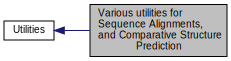
\includegraphics[width=303pt]{group__aln__utils}
\end{center}
\end{figure}
\subsection*{Files}
\begin{DoxyCompactItemize}
\item 
file \hyperlink{aln__util_8h}{aln\+\_\+util.\+h}
\begin{DoxyCompactList}\small\item\em Various utility-\/ and helper-\/functions for sequence alignments and comparative structure prediction. \end{DoxyCompactList}\end{DoxyCompactItemize}
\subsection*{Data Structures}
\begin{DoxyCompactItemize}
\item 
struct \hyperlink{group__aln__utils_structvrna__pinfo__s}{vrna\+\_\+pinfo\+\_\+s}
\begin{DoxyCompactList}\small\item\em A base pair info structure.  \hyperlink{group__aln__utils_structvrna__pinfo__s}{More...}\end{DoxyCompactList}\end{DoxyCompactItemize}
\subsection*{Typedefs}
\begin{DoxyCompactItemize}
\item 
\hypertarget{group__aln__utils_ga6660dfca23debee7306e0cd53341263f}{}typedef struct \hyperlink{group__aln__utils_structvrna__pinfo__s}{vrna\+\_\+pinfo\+\_\+s} \hyperlink{group__aln__utils_ga6660dfca23debee7306e0cd53341263f}{vrna\+\_\+pinfo\+\_\+t}\label{group__aln__utils_ga6660dfca23debee7306e0cd53341263f}

\begin{DoxyCompactList}\small\item\em Typename for the base pair info repesenting data structure \hyperlink{group__aln__utils_structvrna__pinfo__s}{vrna\+\_\+pinfo\+\_\+s}. \end{DoxyCompactList}\item 
typedef struct \hyperlink{group__aln__utils_structvrna__pinfo__s}{vrna\+\_\+pinfo\+\_\+s} \hyperlink{group__aln__utils_ga7b61662a793ad0aa1ea38efc3a5baacc}{pair\+\_\+info}
\begin{DoxyCompactList}\small\item\em Old typename of \hyperlink{group__aln__utils_structvrna__pinfo__s}{vrna\+\_\+pinfo\+\_\+s}. \end{DoxyCompactList}\end{DoxyCompactItemize}
\subsection*{Functions}
\begin{DoxyCompactItemize}
\item 
\hyperlink{group__aln__utils_ga6660dfca23debee7306e0cd53341263f}{vrna\+\_\+pinfo\+\_\+t} $\ast$ \hyperlink{group__aln__utils_gaf6421a1318586c59fea6a127ed9f65f3}{vrna\+\_\+aln\+\_\+pinfo} (\hyperlink{group__fold__compound_ga1b0cef17fd40466cef5968eaeeff6166}{vrna\+\_\+fold\+\_\+compound\+\_\+t} $\ast$vc, const char $\ast$structure, double threshold)
\begin{DoxyCompactList}\small\item\em Retrieve an array of \hyperlink{group__aln__utils_ga6660dfca23debee7306e0cd53341263f}{vrna\+\_\+pinfo\+\_\+t} structures from precomputed pair probabilities. \end{DoxyCompactList}\end{DoxyCompactItemize}


\subsection{Detailed Description}


\subsection{Data Structure Documentation}
\index{vrna\+\_\+pinfo\+\_\+s@{vrna\+\_\+pinfo\+\_\+s}}\label{structvrna__pinfo__s}
\hypertarget{group__aln__utils_structvrna__pinfo__s}{}
\subsubsection{struct vrna\+\_\+pinfo\+\_\+s}
A base pair info structure. 

For each base pair (i,j) with i,j in \mbox{[}0, n-\/1\mbox{]} the structure lists\+:
\begin{DoxyItemize}
\item its probability \textquotesingle{}p\textquotesingle{}
\item an entropy-\/like measure for its well-\/definedness \textquotesingle{}ent\textquotesingle{}
\item the frequency of each type of pair in \textquotesingle{}bp\mbox{[}\mbox{]}\textquotesingle{}
\begin{DoxyItemize}
\item \textquotesingle{}bp\mbox{[}0\mbox{]}\textquotesingle{} contains the number of non-\/compatible sequences
\item \textquotesingle{}bp\mbox{[}1\mbox{]}\textquotesingle{} the number of C\+G pairs, etc. 
\end{DoxyItemize}
\end{DoxyItemize}\subsubsection*{Data Fields}
\begin{DoxyCompactItemize}
\item 
\hypertarget{group__aln__utils_ab91db0a87ef8402dc151795ba5a64c6f}{}unsigned \hyperlink{group__aln__utils_ab91db0a87ef8402dc151795ba5a64c6f}{i}\label{group__aln__utils_ab91db0a87ef8402dc151795ba5a64c6f}

\begin{DoxyCompactList}\small\item\em nucleotide position i \end{DoxyCompactList}\item 
\hypertarget{group__aln__utils_a4142e38d6ba127acccdf680300a88e1f}{}unsigned \hyperlink{group__aln__utils_a4142e38d6ba127acccdf680300a88e1f}{j}\label{group__aln__utils_a4142e38d6ba127acccdf680300a88e1f}

\begin{DoxyCompactList}\small\item\em nucleotide position j \end{DoxyCompactList}\item 
\hypertarget{group__aln__utils_a71990eae41fa100db8b557e4512ec281}{}float \hyperlink{group__aln__utils_a71990eae41fa100db8b557e4512ec281}{p}\label{group__aln__utils_a71990eae41fa100db8b557e4512ec281}

\begin{DoxyCompactList}\small\item\em Probability. \end{DoxyCompactList}\item 
\hypertarget{group__aln__utils_a5ab2a63f3da8e12c6d54d8e9dd9e3e73}{}float \hyperlink{group__aln__utils_a5ab2a63f3da8e12c6d54d8e9dd9e3e73}{ent}\label{group__aln__utils_a5ab2a63f3da8e12c6d54d8e9dd9e3e73}

\begin{DoxyCompactList}\small\item\em Pseudo entropy for $ p(i,j) = S_i + S_j - p_ij*ln(p_ij) $. \end{DoxyCompactList}\item 
\hypertarget{group__aln__utils_aa5feac5559b36dcd7cb38111c45d444d}{}short \hyperlink{group__aln__utils_aa5feac5559b36dcd7cb38111c45d444d}{bp} \mbox{[}8\mbox{]}\label{group__aln__utils_aa5feac5559b36dcd7cb38111c45d444d}

\begin{DoxyCompactList}\small\item\em Frequencies of pair\+\_\+types. \end{DoxyCompactList}\item 
\hypertarget{group__aln__utils_a0720ae74ce53802a759ee9f98e9c8c43}{}char \hyperlink{group__aln__utils_a0720ae74ce53802a759ee9f98e9c8c43}{comp}\label{group__aln__utils_a0720ae74ce53802a759ee9f98e9c8c43}

\begin{DoxyCompactList}\small\item\em 1 iff pair is in mfe structure \end{DoxyCompactList}\end{DoxyCompactItemize}


\subsection{Typedef Documentation}
\hypertarget{group__aln__utils_ga7b61662a793ad0aa1ea38efc3a5baacc}{}\index{Various utilities for Sequence Alignments, and Comparative Structure Prediction@{Various utilities for Sequence Alignments, and Comparative Structure Prediction}!pair\+\_\+info@{pair\+\_\+info}}
\index{pair\+\_\+info@{pair\+\_\+info}!Various utilities for Sequence Alignments, and Comparative Structure Prediction@{Various utilities for Sequence Alignments, and Comparative Structure Prediction}}
\subsubsection[{pair\+\_\+info}]{\setlength{\rightskip}{0pt plus 5cm}typedef struct {\bf vrna\+\_\+pinfo\+\_\+s} {\bf pair\+\_\+info}}\label{group__aln__utils_ga7b61662a793ad0aa1ea38efc3a5baacc}


{\ttfamily \#include $<$\hyperlink{aln__util_8h}{Vienna\+R\+N\+A/aln\+\_\+util.\+h}$>$}



Old typename of \hyperlink{group__aln__utils_structvrna__pinfo__s}{vrna\+\_\+pinfo\+\_\+s}. 

\begin{DoxyRefDesc}{Deprecated}
\item[\hyperlink{deprecated__deprecated000026}{Deprecated}]Use \hyperlink{group__aln__utils_ga6660dfca23debee7306e0cd53341263f}{vrna\+\_\+pinfo\+\_\+t} instead! \end{DoxyRefDesc}


\subsection{Function Documentation}
\hypertarget{group__aln__utils_gaf6421a1318586c59fea6a127ed9f65f3}{}\index{Various utilities for Sequence Alignments, and Comparative Structure Prediction@{Various utilities for Sequence Alignments, and Comparative Structure Prediction}!vrna\+\_\+aln\+\_\+pinfo@{vrna\+\_\+aln\+\_\+pinfo}}
\index{vrna\+\_\+aln\+\_\+pinfo@{vrna\+\_\+aln\+\_\+pinfo}!Various utilities for Sequence Alignments, and Comparative Structure Prediction@{Various utilities for Sequence Alignments, and Comparative Structure Prediction}}
\subsubsection[{vrna\+\_\+aln\+\_\+pinfo}]{\setlength{\rightskip}{0pt plus 5cm}{\bf vrna\+\_\+pinfo\+\_\+t}$\ast$ vrna\+\_\+aln\+\_\+pinfo (
\begin{DoxyParamCaption}
\item[{{\bf vrna\+\_\+fold\+\_\+compound\+\_\+t} $\ast$}]{vc, }
\item[{const char $\ast$}]{structure, }
\item[{double}]{threshold}
\end{DoxyParamCaption}
)}\label{group__aln__utils_gaf6421a1318586c59fea6a127ed9f65f3}


{\ttfamily \#include $<$\hyperlink{aln__util_8h}{Vienna\+R\+N\+A/aln\+\_\+util.\+h}$>$}



Retrieve an array of \hyperlink{group__aln__utils_ga6660dfca23debee7306e0cd53341263f}{vrna\+\_\+pinfo\+\_\+t} structures from precomputed pair probabilities. 

This array of structures contains information about positionwise pair probabilies, base pair entropy and more

\begin{DoxySeeAlso}{See also}
\hyperlink{group__aln__utils_ga6660dfca23debee7306e0cd53341263f}{vrna\+\_\+pinfo\+\_\+t}, and \hyperlink{group__pf__fold_ga29e256d688ad221b78d37f427e0e99bc}{vrna\+\_\+pf()}
\end{DoxySeeAlso}

\begin{DoxyParams}{Parameters}
{\em vc} & The \hyperlink{group__fold__compound_ga1b0cef17fd40466cef5968eaeeff6166}{vrna\+\_\+fold\+\_\+compound\+\_\+t} of type \hyperlink{group__fold__compound_gga01a4ff86fa71deaaa5d1abbd95a1447da056345f1bcfe7cd595d1fd437c05246d}{V\+R\+N\+A\+\_\+\+V\+C\+\_\+\+T\+Y\+P\+E\+\_\+\+A\+L\+I\+G\+N\+M\+E\+N\+T} with precomputed partition function matrices \\
\hline
{\em structure} & An optional structure in dot-\/bracket notation (Maybe N\+U\+L\+L) \\
\hline
{\em threshold} & Do not include results with pair probabilities below threshold \\
\hline
\end{DoxyParams}
\begin{DoxyReturn}{Returns}
The \hyperlink{group__aln__utils_ga6660dfca23debee7306e0cd53341263f}{vrna\+\_\+pinfo\+\_\+t} array 
\end{DoxyReturn}

\hypertarget{group__file__utils}{\section{Functions to Read/\+Write several File Formats for R\+N\+A Sequences, Structures, and Alignments}
\label{group__file__utils}\index{Functions to Read/\+Write several File Formats for R\+N\+A Sequences, Structures, and Alignments@{Functions to Read/\+Write several File Formats for R\+N\+A Sequences, Structures, and Alignments}}
}
Collaboration diagram for Functions to Read/\+Write several File Formats for R\+N\+A Sequences, Structures, and Alignments\+:
\nopagebreak
\begin{figure}[H]
\begin{center}
\leavevmode
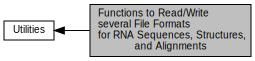
\includegraphics[width=327pt]{group__file__utils}
\end{center}
\end{figure}
\subsection*{Files}
\begin{DoxyCompactItemize}
\item 
file \hyperlink{file__formats_8h}{file\+\_\+formats.\+h}
\begin{DoxyCompactList}\small\item\em Functions dealing with file formats for R\+N\+A sequences, structures, and alignments. \end{DoxyCompactList}\item 
file \hyperlink{ribo_8h}{ribo.\+h}
\begin{DoxyCompactList}\small\item\em Parse Ribo\+Sum Scoring Matrices for Covariance Scoring of Alignments. \end{DoxyCompactList}\end{DoxyCompactItemize}
\subsection*{Functions}
\begin{DoxyCompactItemize}
\item 
void \hyperlink{group__file__utils_gaaface7db12fadc3d271641c4515ab6e4}{vrna\+\_\+file\+\_\+helixlist} (const char $\ast$seq, const char $\ast$db, float energy, F\+I\+L\+E $\ast$file)
\begin{DoxyCompactList}\small\item\em Print a secondary structure as helix list. \end{DoxyCompactList}\item 
void \hyperlink{group__file__utils_gab69682373ccca1e0e28cc967eec07745}{vrna\+\_\+file\+\_\+connect} (const char $\ast$seq, const char $\ast$db, float energy, const char $\ast$identifier, F\+I\+L\+E $\ast$file)
\begin{DoxyCompactList}\small\item\em Print a secondary structure as connect table. \end{DoxyCompactList}\item 
void \hyperlink{group__file__utils_ga9b462e6f202594af5d3fa56e280d633f}{vrna\+\_\+file\+\_\+bpseq} (const char $\ast$seq, const char $\ast$db, F\+I\+L\+E $\ast$file)
\begin{DoxyCompactList}\small\item\em Print a secondary structure in bpseq format. \end{DoxyCompactList}\item 
void \hyperlink{group__file__utils_ga31f4a6c2ea1495a6e4f9eb45a9f6193d}{vrna\+\_\+file\+\_\+json} (const char $\ast$seq, const char $\ast$db, double energy, const char $\ast$identifier, F\+I\+L\+E $\ast$file)
\begin{DoxyCompactList}\small\item\em Print a secondary structure in jsonformat. \end{DoxyCompactList}\item 
unsigned int \hyperlink{group__file__utils_ga8cfb7e271efc9e1f34640acb85475639}{vrna\+\_\+file\+\_\+fasta\+\_\+read\+\_\+record} (char $\ast$$\ast$header, char $\ast$$\ast$sequence, char $\ast$$\ast$$\ast$rest, F\+I\+L\+E $\ast$file, unsigned int options)
\begin{DoxyCompactList}\small\item\em Get a (fasta) data set from a file or stdin. \end{DoxyCompactList}\item 
void \hyperlink{group__file__utils_ga55a9ae6dfeecc1b3f0c2acf6fa796c15}{vrna\+\_\+extract\+\_\+record\+\_\+rest\+\_\+constraint} (char $\ast$$\ast$cstruc, const char $\ast$$\ast$lines, unsigned int option)
\begin{DoxyCompactList}\small\item\em Extract a hard constraint encoded as pseudo dot-\/bracket string. \end{DoxyCompactList}\item 
int \hyperlink{group__file__utils_ga646ebf45450a69a7f2533f9ecd283a32}{vrna\+\_\+file\+\_\+\+S\+H\+A\+P\+E\+\_\+read} (const char $\ast$file\+\_\+name, int length, double default\+\_\+value, char $\ast$sequence, double $\ast$values)
\begin{DoxyCompactList}\small\item\em Read data from a given S\+H\+A\+P\+E reactivity input file. \end{DoxyCompactList}\item 
\hyperlink{group__data__structures_ga8e4eb5e1bfc95776559575beb359af87}{vrna\+\_\+plist\+\_\+t} $\ast$ \hyperlink{group__file__utils_gae33323c53765ecbbc410d9de2d495432}{vrna\+\_\+file\+\_\+constraints\+\_\+read} (const char $\ast$filename, unsigned int length, unsigned int options)
\begin{DoxyCompactList}\small\item\em Read constraints from an input file. \end{DoxyCompactList}\item 
unsigned int \hyperlink{group__file__utils_gafd194a69af9d92b5b0412a7627ac1595}{read\+\_\+record} (char $\ast$$\ast$header, char $\ast$$\ast$sequence, char $\ast$$\ast$$\ast$rest, unsigned int options)
\begin{DoxyCompactList}\small\item\em Get a data record from stdin. \end{DoxyCompactList}\item 
\hypertarget{group__file__utils_ga5e125c9586fcd4e2e1559fe76f7289cc}{float $\ast$$\ast$ \hyperlink{group__file__utils_ga5e125c9586fcd4e2e1559fe76f7289cc}{readribosum} (char $\ast$name)}\label{group__file__utils_ga5e125c9586fcd4e2e1559fe76f7289cc}

\begin{DoxyCompactList}\small\item\em Read a Ribo\+Sum or other user-\/defined Scoring Matrix and Store into global Memory. \end{DoxyCompactList}\end{DoxyCompactItemize}


\subsection{Detailed Description}


\subsection{Function Documentation}
\hypertarget{group__file__utils_gaaface7db12fadc3d271641c4515ab6e4}{\index{Functions to Read/\+Write several File Formats for R\+N\+A Sequences, Structures, and Alignments@{Functions to Read/\+Write several File Formats for R\+N\+A Sequences, Structures, and Alignments}!vrna\+\_\+file\+\_\+helixlist@{vrna\+\_\+file\+\_\+helixlist}}
\index{vrna\+\_\+file\+\_\+helixlist@{vrna\+\_\+file\+\_\+helixlist}!Functions to Read/\+Write several File Formats for R\+N\+A Sequences, Structures, and Alignments@{Functions to Read/\+Write several File Formats for R\+N\+A Sequences, Structures, and Alignments}}
\subsubsection[{vrna\+\_\+file\+\_\+helixlist}]{\setlength{\rightskip}{0pt plus 5cm}void vrna\+\_\+file\+\_\+helixlist (
\begin{DoxyParamCaption}
\item[{const char $\ast$}]{seq, }
\item[{const char $\ast$}]{db, }
\item[{float}]{energy, }
\item[{F\+I\+L\+E $\ast$}]{file}
\end{DoxyParamCaption}
)}}\label{group__file__utils_gaaface7db12fadc3d271641c4515ab6e4}


{\ttfamily \#include $<$\hyperlink{file__formats_8h}{Vienna\+R\+N\+A/file\+\_\+formats.\+h}$>$}



Print a secondary structure as helix list. 


\begin{DoxyParams}{Parameters}
{\em seq} & The R\+N\+A sequence \\
\hline
{\em db} & The structure in dot-\/bracket format \\
\hline
{\em file} & The file handle used to print to (print defaults to 'stdout' if(file == N\+U\+L\+L) ) \\
\hline
\end{DoxyParams}
\hypertarget{group__file__utils_gab69682373ccca1e0e28cc967eec07745}{\index{Functions to Read/\+Write several File Formats for R\+N\+A Sequences, Structures, and Alignments@{Functions to Read/\+Write several File Formats for R\+N\+A Sequences, Structures, and Alignments}!vrna\+\_\+file\+\_\+connect@{vrna\+\_\+file\+\_\+connect}}
\index{vrna\+\_\+file\+\_\+connect@{vrna\+\_\+file\+\_\+connect}!Functions to Read/\+Write several File Formats for R\+N\+A Sequences, Structures, and Alignments@{Functions to Read/\+Write several File Formats for R\+N\+A Sequences, Structures, and Alignments}}
\subsubsection[{vrna\+\_\+file\+\_\+connect}]{\setlength{\rightskip}{0pt plus 5cm}void vrna\+\_\+file\+\_\+connect (
\begin{DoxyParamCaption}
\item[{const char $\ast$}]{seq, }
\item[{const char $\ast$}]{db, }
\item[{float}]{energy, }
\item[{const char $\ast$}]{identifier, }
\item[{F\+I\+L\+E $\ast$}]{file}
\end{DoxyParamCaption}
)}}\label{group__file__utils_gab69682373ccca1e0e28cc967eec07745}


{\ttfamily \#include $<$\hyperlink{file__formats_8h}{Vienna\+R\+N\+A/file\+\_\+formats.\+h}$>$}



Print a secondary structure as connect table. 

Connect table file format looks like this\+: \begin{DoxyVerb}300  ENERGY = 7.0  example
  1 G       0    2   22    1
  2 G       1    3   21    2
\end{DoxyVerb}
 where the headerline is followed by 6 columns with\+:
\begin{DoxyEnumerate}
\item Base number\+: index n
\item Base (A, C, G, T, U, X)
\item Index n-\/1 (0 if first nucleotide)
\item Index n+1 (0 if last nucleotide)
\item Number of the base to which n is paired. No pairing is indicated by 0 (zero).
\item Natural numbering.
\end{DoxyEnumerate}


\begin{DoxyParams}{Parameters}
{\em seq} & The R\+N\+A sequence \\
\hline
{\em db} & The structure in dot-\/bracket format \\
\hline
{\em energy} & The free energy of the structure \\
\hline
{\em identifier} & An optional identifier for the sequence \\
\hline
{\em file} & The file handle used to print to (print defaults to 'stdout' if(file == N\+U\+L\+L) ) \\
\hline
\end{DoxyParams}
\hypertarget{group__file__utils_ga9b462e6f202594af5d3fa56e280d633f}{\index{Functions to Read/\+Write several File Formats for R\+N\+A Sequences, Structures, and Alignments@{Functions to Read/\+Write several File Formats for R\+N\+A Sequences, Structures, and Alignments}!vrna\+\_\+file\+\_\+bpseq@{vrna\+\_\+file\+\_\+bpseq}}
\index{vrna\+\_\+file\+\_\+bpseq@{vrna\+\_\+file\+\_\+bpseq}!Functions to Read/\+Write several File Formats for R\+N\+A Sequences, Structures, and Alignments@{Functions to Read/\+Write several File Formats for R\+N\+A Sequences, Structures, and Alignments}}
\subsubsection[{vrna\+\_\+file\+\_\+bpseq}]{\setlength{\rightskip}{0pt plus 5cm}void vrna\+\_\+file\+\_\+bpseq (
\begin{DoxyParamCaption}
\item[{const char $\ast$}]{seq, }
\item[{const char $\ast$}]{db, }
\item[{F\+I\+L\+E $\ast$}]{file}
\end{DoxyParamCaption}
)}}\label{group__file__utils_ga9b462e6f202594af5d3fa56e280d633f}


{\ttfamily \#include $<$\hyperlink{file__formats_8h}{Vienna\+R\+N\+A/file\+\_\+formats.\+h}$>$}



Print a secondary structure in bpseq format. 


\begin{DoxyParams}{Parameters}
{\em seq} & The R\+N\+A sequence \\
\hline
{\em db} & The structure in dot-\/bracket format \\
\hline
{\em file} & The file handle used to print to (print defaults to 'stdout' if(file == N\+U\+L\+L) ) \\
\hline
\end{DoxyParams}
\hypertarget{group__file__utils_ga31f4a6c2ea1495a6e4f9eb45a9f6193d}{\index{Functions to Read/\+Write several File Formats for R\+N\+A Sequences, Structures, and Alignments@{Functions to Read/\+Write several File Formats for R\+N\+A Sequences, Structures, and Alignments}!vrna\+\_\+file\+\_\+json@{vrna\+\_\+file\+\_\+json}}
\index{vrna\+\_\+file\+\_\+json@{vrna\+\_\+file\+\_\+json}!Functions to Read/\+Write several File Formats for R\+N\+A Sequences, Structures, and Alignments@{Functions to Read/\+Write several File Formats for R\+N\+A Sequences, Structures, and Alignments}}
\subsubsection[{vrna\+\_\+file\+\_\+json}]{\setlength{\rightskip}{0pt plus 5cm}void vrna\+\_\+file\+\_\+json (
\begin{DoxyParamCaption}
\item[{const char $\ast$}]{seq, }
\item[{const char $\ast$}]{db, }
\item[{double}]{energy, }
\item[{const char $\ast$}]{identifier, }
\item[{F\+I\+L\+E $\ast$}]{file}
\end{DoxyParamCaption}
)}}\label{group__file__utils_ga31f4a6c2ea1495a6e4f9eb45a9f6193d}


{\ttfamily \#include $<$\hyperlink{file__formats_8h}{Vienna\+R\+N\+A/file\+\_\+formats.\+h}$>$}



Print a secondary structure in jsonformat. 


\begin{DoxyParams}{Parameters}
{\em seq} & The R\+N\+A sequence \\
\hline
{\em db} & The structure in dot-\/bracket format \\
\hline
{\em energy} & The free energy \\
\hline
{\em identifier} & An identifier for the sequence \\
\hline
{\em file} & The file handle used to print to (print defaults to 'stdout' if(file == N\+U\+L\+L) ) \\
\hline
\end{DoxyParams}
\hypertarget{group__file__utils_ga8cfb7e271efc9e1f34640acb85475639}{\index{Functions to Read/\+Write several File Formats for R\+N\+A Sequences, Structures, and Alignments@{Functions to Read/\+Write several File Formats for R\+N\+A Sequences, Structures, and Alignments}!vrna\+\_\+file\+\_\+fasta\+\_\+read\+\_\+record@{vrna\+\_\+file\+\_\+fasta\+\_\+read\+\_\+record}}
\index{vrna\+\_\+file\+\_\+fasta\+\_\+read\+\_\+record@{vrna\+\_\+file\+\_\+fasta\+\_\+read\+\_\+record}!Functions to Read/\+Write several File Formats for R\+N\+A Sequences, Structures, and Alignments@{Functions to Read/\+Write several File Formats for R\+N\+A Sequences, Structures, and Alignments}}
\subsubsection[{vrna\+\_\+file\+\_\+fasta\+\_\+read\+\_\+record}]{\setlength{\rightskip}{0pt plus 5cm}unsigned int vrna\+\_\+file\+\_\+fasta\+\_\+read\+\_\+record (
\begin{DoxyParamCaption}
\item[{char $\ast$$\ast$}]{header, }
\item[{char $\ast$$\ast$}]{sequence, }
\item[{char $\ast$$\ast$$\ast$}]{rest, }
\item[{F\+I\+L\+E $\ast$}]{file, }
\item[{unsigned int}]{options}
\end{DoxyParamCaption}
)}}\label{group__file__utils_ga8cfb7e271efc9e1f34640acb85475639}


{\ttfamily \#include $<$\hyperlink{file__formats_8h}{Vienna\+R\+N\+A/file\+\_\+formats.\+h}$>$}



Get a (fasta) data set from a file or stdin. 

This function may be used to obtain complete datasets from a filehandle or stdin. A dataset is always defined to contain at least a sequence. If data starts with a fasta header, i.\+e. a line like \begin{DoxyVerb}>some header info \end{DoxyVerb}
 then \hyperlink{group__file__utils_ga8cfb7e271efc9e1f34640acb85475639}{vrna\+\_\+file\+\_\+fasta\+\_\+read\+\_\+record()} will assume that the sequence that follows the header may span over several lines. To disable this behavior and to assign a single line to the argument 'sequence' one can pass \hyperlink{group__utils_ga0de536599b881c787b0943a2671da476}{V\+R\+N\+A\+\_\+\+I\+N\+P\+U\+T\+\_\+\+N\+O\+\_\+\+S\+P\+A\+N} in the 'options' argument. If no fasta header is read in the beginning of a data block, a sequence must not span over multiple lines!~\newline
 Unless the options \hyperlink{group__utils_ga0f6311f11bed1842e3a527ab27b294c6}{V\+R\+N\+A\+\_\+\+I\+N\+P\+U\+T\+\_\+\+N\+O\+S\+K\+I\+P\+\_\+\+C\+O\+M\+M\+E\+N\+T\+S} or \hyperlink{group__utils_gab4db885222b3b69608310d7c7e63e286}{V\+R\+N\+A\+\_\+\+I\+N\+P\+U\+T\+\_\+\+N\+O\+S\+K\+I\+P\+\_\+\+B\+L\+A\+N\+K\+\_\+\+L\+I\+N\+E\+S} are passed, a sequence may be interrupted by lines starting with a comment character or empty lines.~\newline
 A sequence is regarded as completely read if it was either assumed to not span over multiple lines, a secondary structure or structure constraint follows the sequence on the next line, or a new header marks the beginning of a new sequence...~\newline
 All lines following the sequence (this includes comments) that do not initiate a new dataset according to the above definition are available through the line-\/array 'rest'. Here one can usually find the structure constraint or other information belonging to the current dataset. Filling of 'rest' may be prevented by passing \hyperlink{group__utils_ga7a2e8c50a0c7ce82e60da1016e1367fd}{V\+R\+N\+A\+\_\+\+I\+N\+P\+U\+T\+\_\+\+N\+O\+\_\+\+R\+E\+S\+T} to the options argument.~\newline
 \begin{DoxyNote}{Note}
This function will exit any program with an error message if no sequence could be read! 

This function is N\+O\+T threadsafe! It uses a global variable to store information about the next data block.
\end{DoxyNote}
The main purpose of this function is to be able to easily parse blocks of data in the header of a loop where all calculations for the appropriate data is done inside the loop. The loop may be then left on certain return values, e.\+g.\+: 
\begin{DoxyCode}
00001 char *id, *seq, **rest;
00002 int  i;
00003 id = seq = NULL;
00004 rest = NULL;
00005 while(!(vrna\_file\_fasta\_read\_record(&id, &seq, &rest, NULL, 0) & (VRNA\_INPUT\_ERROR |
       VRNA\_INPUT\_QUIT)))\{
00006   if(id) printf("%s\(\backslash\)n", id);
00007   printf("%s\(\backslash\)n", seq);
00008   if(rest)
00009     for(i=0;rest[i];i++)\{
00010       printf("%s\(\backslash\)n", rest[i]);
00011       free(rest[i]);
00012     \}
00013   free(rest);
00014   free(seq);
00015   free(id);
00016 \}
\end{DoxyCode}
 In the example above, the while loop will be terminated when \hyperlink{group__file__utils_ga8cfb7e271efc9e1f34640acb85475639}{vrna\+\_\+file\+\_\+fasta\+\_\+read\+\_\+record()} returns either an error, E\+O\+F, or a user initiated quit request.~\newline
 As long as data is read from stdin (we are passing N\+U\+L\+L as the file pointer), the id is printed if it is available for the current block of data. The sequence will be printed in any case and if some more lines belong to the current block of data each line will be printed as well.

\begin{DoxyNote}{Note}
Do not forget to free the memory occupied by header, sequence and rest!
\end{DoxyNote}

\begin{DoxyParams}{Parameters}
{\em header} & A pointer which will be set such that it points to the header of the record \\
\hline
{\em sequence} & A pointer which will be set such that it points to the sequence of the record \\
\hline
{\em rest} & A pointer which will be set such that it points to an array of lines which also belong to the record \\
\hline
{\em file} & A file handle to read from (if N\+U\+L\+L, this function reads from stdin) \\
\hline
{\em options} & Some options which may be passed to alter the behavior of the function, use 0 for no options \\
\hline
\end{DoxyParams}
\begin{DoxyReturn}{Returns}
A flag with information about what the function actually did read 
\end{DoxyReturn}
\hypertarget{group__file__utils_ga55a9ae6dfeecc1b3f0c2acf6fa796c15}{\index{Functions to Read/\+Write several File Formats for R\+N\+A Sequences, Structures, and Alignments@{Functions to Read/\+Write several File Formats for R\+N\+A Sequences, Structures, and Alignments}!vrna\+\_\+extract\+\_\+record\+\_\+rest\+\_\+constraint@{vrna\+\_\+extract\+\_\+record\+\_\+rest\+\_\+constraint}}
\index{vrna\+\_\+extract\+\_\+record\+\_\+rest\+\_\+constraint@{vrna\+\_\+extract\+\_\+record\+\_\+rest\+\_\+constraint}!Functions to Read/\+Write several File Formats for R\+N\+A Sequences, Structures, and Alignments@{Functions to Read/\+Write several File Formats for R\+N\+A Sequences, Structures, and Alignments}}
\subsubsection[{vrna\+\_\+extract\+\_\+record\+\_\+rest\+\_\+constraint}]{\setlength{\rightskip}{0pt plus 5cm}void vrna\+\_\+extract\+\_\+record\+\_\+rest\+\_\+constraint (
\begin{DoxyParamCaption}
\item[{char $\ast$$\ast$}]{cstruc, }
\item[{const char $\ast$$\ast$}]{lines, }
\item[{unsigned int}]{option}
\end{DoxyParamCaption}
)}}\label{group__file__utils_ga55a9ae6dfeecc1b3f0c2acf6fa796c15}


{\ttfamily \#include $<$\hyperlink{file__formats_8h}{Vienna\+R\+N\+A/file\+\_\+formats.\+h}$>$}



Extract a hard constraint encoded as pseudo dot-\/bracket string. 

\begin{DoxyPrecond}{Precondition}
The argument 'lines' has to be a 2-\/dimensional character array as obtained by \hyperlink{group__file__utils_ga8cfb7e271efc9e1f34640acb85475639}{vrna\+\_\+file\+\_\+fasta\+\_\+read\+\_\+record()} 
\end{DoxyPrecond}
\begin{DoxySeeAlso}{See also}
\hyperlink{group__file__utils_ga8cfb7e271efc9e1f34640acb85475639}{vrna\+\_\+file\+\_\+fasta\+\_\+read\+\_\+record()}, \hyperlink{group__constraints_ga13053547a2de5532b64b64d35e097ae1}{V\+R\+N\+A\+\_\+\+C\+O\+N\+S\+T\+R\+A\+I\+N\+T\+\_\+\+D\+B\+\_\+\+P\+I\+P\+E}, \hyperlink{group__constraints_ga369bea82eae75fbe626f409fa425747e}{V\+R\+N\+A\+\_\+\+C\+O\+N\+S\+T\+R\+A\+I\+N\+T\+\_\+\+D\+B\+\_\+\+D\+O\+T}, \hyperlink{group__constraints_ga7283bbe0f8954f7b030ecc3f2d1932b2}{V\+R\+N\+A\+\_\+\+C\+O\+N\+S\+T\+R\+A\+I\+N\+T\+\_\+\+D\+B\+\_\+\+X} \hyperlink{group__constraints_gad54c1315a47d55653dcaa5de6e544b77}{V\+R\+N\+A\+\_\+\+C\+O\+N\+S\+T\+R\+A\+I\+N\+T\+\_\+\+D\+B\+\_\+\+A\+N\+G\+\_\+\+B\+R\+A\+C\+K}, \hyperlink{group__constraints_gac17b034852c914bc5879954c65d7e74b}{V\+R\+N\+A\+\_\+\+C\+O\+N\+S\+T\+R\+A\+I\+N\+T\+\_\+\+D\+B\+\_\+\+R\+N\+D\+\_\+\+B\+R\+A\+C\+K}
\end{DoxySeeAlso}

\begin{DoxyParams}{Parameters}
{\em cstruc} & A pointer to a character array that is used as pseudo dot-\/bracket output \\
\hline
{\em lines} & A 2-\/dimensional character array with the extension lines from the F\+A\+S\+T\+A input \\
\hline
{\em option} & The option flags that define the behavior and recognition pattern of this function \\
\hline
\end{DoxyParams}
\hypertarget{group__file__utils_ga646ebf45450a69a7f2533f9ecd283a32}{\index{Functions to Read/\+Write several File Formats for R\+N\+A Sequences, Structures, and Alignments@{Functions to Read/\+Write several File Formats for R\+N\+A Sequences, Structures, and Alignments}!vrna\+\_\+file\+\_\+\+S\+H\+A\+P\+E\+\_\+read@{vrna\+\_\+file\+\_\+\+S\+H\+A\+P\+E\+\_\+read}}
\index{vrna\+\_\+file\+\_\+\+S\+H\+A\+P\+E\+\_\+read@{vrna\+\_\+file\+\_\+\+S\+H\+A\+P\+E\+\_\+read}!Functions to Read/\+Write several File Formats for R\+N\+A Sequences, Structures, and Alignments@{Functions to Read/\+Write several File Formats for R\+N\+A Sequences, Structures, and Alignments}}
\subsubsection[{vrna\+\_\+file\+\_\+\+S\+H\+A\+P\+E\+\_\+read}]{\setlength{\rightskip}{0pt plus 5cm}int vrna\+\_\+file\+\_\+\+S\+H\+A\+P\+E\+\_\+read (
\begin{DoxyParamCaption}
\item[{const char $\ast$}]{file\+\_\+name, }
\item[{int}]{length, }
\item[{double}]{default\+\_\+value, }
\item[{char $\ast$}]{sequence, }
\item[{double $\ast$}]{values}
\end{DoxyParamCaption}
)}}\label{group__file__utils_ga646ebf45450a69a7f2533f9ecd283a32}


{\ttfamily \#include $<$\hyperlink{file__formats_8h}{Vienna\+R\+N\+A/file\+\_\+formats.\+h}$>$}



Read data from a given S\+H\+A\+P\+E reactivity input file. 

This function parses the informations from a given file and stores the result in the preallocated string sequence and the double array values.


\begin{DoxyParams}{Parameters}
{\em file\+\_\+name} & Path to the constraints file \\
\hline
{\em length} & Length of the sequence (file entries exceeding this limit will cause an error) \\
\hline
{\em default\+\_\+value} & Value for missing indices \\
\hline
{\em sequence} & Pointer to an array used for storing the sequence obtained from the S\+H\+A\+P\+E reactivity file \\
\hline
{\em values} & Pointer to an array used for storing the values obtained from the S\+H\+A\+P\+E reactivity file \\
\hline
\end{DoxyParams}
\hypertarget{group__file__utils_gae33323c53765ecbbc410d9de2d495432}{\index{Functions to Read/\+Write several File Formats for R\+N\+A Sequences, Structures, and Alignments@{Functions to Read/\+Write several File Formats for R\+N\+A Sequences, Structures, and Alignments}!vrna\+\_\+file\+\_\+constraints\+\_\+read@{vrna\+\_\+file\+\_\+constraints\+\_\+read}}
\index{vrna\+\_\+file\+\_\+constraints\+\_\+read@{vrna\+\_\+file\+\_\+constraints\+\_\+read}!Functions to Read/\+Write several File Formats for R\+N\+A Sequences, Structures, and Alignments@{Functions to Read/\+Write several File Formats for R\+N\+A Sequences, Structures, and Alignments}}
\subsubsection[{vrna\+\_\+file\+\_\+constraints\+\_\+read}]{\setlength{\rightskip}{0pt plus 5cm}{\bf vrna\+\_\+plist\+\_\+t}$\ast$ vrna\+\_\+file\+\_\+constraints\+\_\+read (
\begin{DoxyParamCaption}
\item[{const char $\ast$}]{filename, }
\item[{unsigned int}]{length, }
\item[{unsigned int}]{options}
\end{DoxyParamCaption}
)}}\label{group__file__utils_gae33323c53765ecbbc410d9de2d495432}


{\ttfamily \#include $<$\hyperlink{file__formats_8h}{Vienna\+R\+N\+A/file\+\_\+formats.\+h}$>$}



Read constraints from an input file. 

This function reads constraint definitions from a file and converts them into an array of \hyperlink{group__data__structures_ga8e4eb5e1bfc95776559575beb359af87}{vrna\+\_\+plist\+\_\+t} data structures. The data fields of each individual returned plist entry may adopt the following configurations\+:
\begin{DoxyItemize}
\item plist.\+i == plist.\+j $ \rightarrow $ single nucleotide constraint
\item plist.\+i != plist.\+j $ \rightarrow $ base pair constraint
\item plist.\+i == 0 $ \rightarrow $ End of list 
\end{DoxyItemize}\hypertarget{group__file__utils_gafd194a69af9d92b5b0412a7627ac1595}{\index{Functions to Read/\+Write several File Formats for R\+N\+A Sequences, Structures, and Alignments@{Functions to Read/\+Write several File Formats for R\+N\+A Sequences, Structures, and Alignments}!read\+\_\+record@{read\+\_\+record}}
\index{read\+\_\+record@{read\+\_\+record}!Functions to Read/\+Write several File Formats for R\+N\+A Sequences, Structures, and Alignments@{Functions to Read/\+Write several File Formats for R\+N\+A Sequences, Structures, and Alignments}}
\subsubsection[{read\+\_\+record}]{\setlength{\rightskip}{0pt plus 5cm}unsigned int read\+\_\+record (
\begin{DoxyParamCaption}
\item[{char $\ast$$\ast$}]{header, }
\item[{char $\ast$$\ast$}]{sequence, }
\item[{char $\ast$$\ast$$\ast$}]{rest, }
\item[{unsigned int}]{options}
\end{DoxyParamCaption}
)}}\label{group__file__utils_gafd194a69af9d92b5b0412a7627ac1595}


{\ttfamily \#include $<$\hyperlink{file__formats_8h}{Vienna\+R\+N\+A/file\+\_\+formats.\+h}$>$}



Get a data record from stdin. 

\begin{DoxyRefDesc}{Deprecated}
\item[\hyperlink{deprecated__deprecated000061}{Deprecated}]This function is deprecated! Use \hyperlink{group__file__utils_ga8cfb7e271efc9e1f34640acb85475639}{vrna\+\_\+file\+\_\+fasta\+\_\+read\+\_\+record()} as a replacment.\end{DoxyRefDesc}

\include{group__plotting__utils}
\chapter{Data Structure Documentation}
\input{struct__struct__en}
\hypertarget{structLIST}{\section{L\+I\+S\+T Struct Reference}
\label{structLIST}\index{L\+I\+S\+T@{L\+I\+S\+T}}
}


Collaboration diagram for L\+I\+S\+T\+:
\nopagebreak
\begin{figure}[H]
\begin{center}
\leavevmode
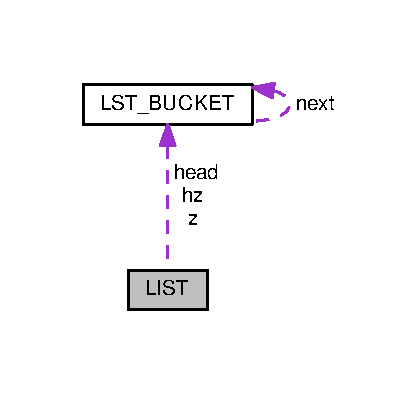
\includegraphics[width=201pt]{structLIST__coll__graph}
\end{center}
\end{figure}


The documentation for this struct was generated from the following file\+:\begin{DoxyCompactItemize}
\item 
Vienna\+R\+N\+A/list.\+h\end{DoxyCompactItemize}

\hypertarget{structLST__BUCKET}{\section{L\+S\+T\+\_\+\+B\+U\+C\+K\+E\+T Struct Reference}
\label{structLST__BUCKET}\index{L\+S\+T\+\_\+\+B\+U\+C\+K\+E\+T@{L\+S\+T\+\_\+\+B\+U\+C\+K\+E\+T}}
}


Collaboration diagram for L\+S\+T\+\_\+\+B\+U\+C\+K\+E\+T\+:
\nopagebreak
\begin{figure}[H]
\begin{center}
\leavevmode
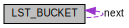
\includegraphics[width=201pt]{structLST__BUCKET__coll__graph}
\end{center}
\end{figure}


The documentation for this struct was generated from the following file\+:\begin{DoxyCompactItemize}
\item 
Vienna\+R\+N\+A/list.\+h\end{DoxyCompactItemize}

\input{structPostorder__list}
\input{structswString}
\hypertarget{structTree}{}\section{Tree Struct Reference}
\label{structTree}\index{Tree@{Tree}}


Collaboration diagram for Tree\+:
\nopagebreak
\begin{figure}[H]
\begin{center}
\leavevmode
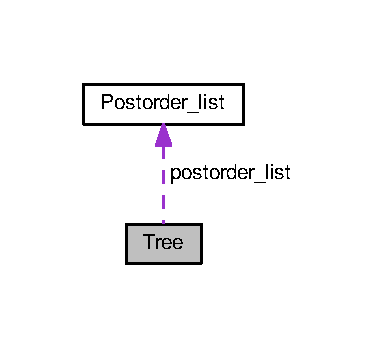
\includegraphics[width=181pt]{structTree__coll__graph}
\end{center}
\end{figure}


The documentation for this struct was generated from the following file\+:\begin{DoxyCompactItemize}
\item 
Vienna\+R\+N\+A/\hyperlink{dist__vars_8h}{dist\+\_\+vars.\+h}\end{DoxyCompactItemize}

\input{structTwoDpfold__vars}
\hypertarget{structvrna__subopt__sol__s}{\section{vrna\+\_\+subopt\+\_\+sol\+\_\+s Struct Reference}
\label{structvrna__subopt__sol__s}\index{vrna\+\_\+subopt\+\_\+sol\+\_\+s@{vrna\+\_\+subopt\+\_\+sol\+\_\+s}}
}


Solution element from subopt.\+c.  


\subsection*{Data Fields}
\begin{DoxyCompactItemize}
\item 
\hypertarget{structvrna__subopt__sol__s_a99bc26ca68392aa4656386cf73b73fef}{float \hyperlink{structvrna__subopt__sol__s_a99bc26ca68392aa4656386cf73b73fef}{energy}}\label{structvrna__subopt__sol__s_a99bc26ca68392aa4656386cf73b73fef}

\begin{DoxyCompactList}\small\item\em Free Energy of structure in kcal/mol. \end{DoxyCompactList}\item 
\hypertarget{structvrna__subopt__sol__s_a3c632c7f08eb6a8827c6151625e5ef8e}{char $\ast$ \hyperlink{structvrna__subopt__sol__s_a3c632c7f08eb6a8827c6151625e5ef8e}{structure}}\label{structvrna__subopt__sol__s_a3c632c7f08eb6a8827c6151625e5ef8e}

\begin{DoxyCompactList}\small\item\em Structure in dot-\/bracket notation. \end{DoxyCompactList}\end{DoxyCompactItemize}


\subsection{Detailed Description}
Solution element from subopt.\+c. 

The documentation for this struct was generated from the following file\+:\begin{DoxyCompactItemize}
\item 
Vienna\+R\+N\+A/\hyperlink{subopt_8h}{subopt.\+h}\end{DoxyCompactItemize}

\chapter{File Documentation}
\input{1_88_84__epars_8h}
\hypertarget{1_88_84__intloops_8h}{}\section{Vienna\+R\+N\+A/1.8.4\+\_\+intloops.h File Reference}
\label{1_88_84__intloops_8h}\index{Vienna\+R\+N\+A/1.\+8.\+4\+\_\+intloops.\+h@{Vienna\+R\+N\+A/1.\+8.\+4\+\_\+intloops.\+h}}


Free energy parameters for interior loop contributions needed by the parameter file conversion functions.  




\subsection{Detailed Description}
Free energy parameters for interior loop contributions needed by the parameter file conversion functions. 


\input{2Dfold_8h}
\hypertarget{2Dpfold_8h}{}\section{Vienna\+R\+N\+A/2\+Dpfold.h File Reference}
\label{2Dpfold_8h}\index{Vienna\+R\+N\+A/2\+Dpfold.\+h@{Vienna\+R\+N\+A/2\+Dpfold.\+h}}
Include dependency graph for 2\+Dpfold.h\+:
\nopagebreak
\begin{figure}[H]
\begin{center}
\leavevmode
\includegraphics[width=350pt]{2Dpfold_8h__incl}
\end{center}
\end{figure}
\subsection*{Data Structures}
\begin{DoxyCompactItemize}
\item 
struct \hyperlink{group__kl__neighborhood__pf_structvrna__sol__TwoD__pf__t}{vrna\+\_\+sol\+\_\+\+Two\+D\+\_\+pf\+\_\+t}
\begin{DoxyCompactList}\small\item\em Solution element returned from \hyperlink{group__kl__neighborhood__pf_ga0bc3427689bd09da09b8b3094a27f836}{vrna\+\_\+pf\+\_\+\+Two\+D()}  \hyperlink{group__kl__neighborhood__pf_structvrna__sol__TwoD__pf__t}{More...}\end{DoxyCompactList}\item 
struct \hyperlink{structTwoDpfold__vars}{Two\+Dpfold\+\_\+vars}
\begin{DoxyCompactList}\small\item\em Variables compound for 2\+Dfold partition function folding. \end{DoxyCompactList}\end{DoxyCompactItemize}
\subsection*{Typedefs}
\begin{DoxyCompactItemize}
\item 
typedef struct \hyperlink{group__kl__neighborhood__pf_structvrna__sol__TwoD__pf__t}{vrna\+\_\+sol\+\_\+\+Two\+D\+\_\+pf\+\_\+t} \hyperlink{group__kl__neighborhood__pf_ga5e449fbd695406aabd2bcabddc374621}{vrna\+\_\+sol\+\_\+\+Two\+D\+\_\+pf\+\_\+t}
\begin{DoxyCompactList}\small\item\em Solution element returned from \hyperlink{group__kl__neighborhood__pf_ga0bc3427689bd09da09b8b3094a27f836}{vrna\+\_\+pf\+\_\+\+Two\+D()} \end{DoxyCompactList}\end{DoxyCompactItemize}
\subsection*{Functions}
\begin{DoxyCompactItemize}
\item 
\hyperlink{group__kl__neighborhood__pf_structvrna__sol__TwoD__pf__t}{vrna\+\_\+sol\+\_\+\+Two\+D\+\_\+pf\+\_\+t} $\ast$ \hyperlink{group__kl__neighborhood__pf_ga0bc3427689bd09da09b8b3094a27f836}{vrna\+\_\+pf\+\_\+\+Two\+D} (\hyperlink{group__fold__compound_ga1b0cef17fd40466cef5968eaeeff6166}{vrna\+\_\+fold\+\_\+compound\+\_\+t} $\ast$vc, int max\+Distance1, int max\+Distance2)
\begin{DoxyCompactList}\small\item\em Compute the partition function for all distance classes. \end{DoxyCompactList}\item 
char $\ast$ \hyperlink{group__kl__neighborhood__stochbt_ga14aceef73f83bbde77bb3a0ca06c9d13}{vrna\+\_\+pbacktrack\+\_\+\+Two\+D} (\hyperlink{group__fold__compound_ga1b0cef17fd40466cef5968eaeeff6166}{vrna\+\_\+fold\+\_\+compound\+\_\+t} $\ast$vc, int d1, int d2)
\begin{DoxyCompactList}\small\item\em Sample secondary structure representatives from a set of distance classes according to their Boltzmann probability. \end{DoxyCompactList}\item 
char $\ast$ \hyperlink{group__kl__neighborhood__stochbt_ga6504913303bc325659c365d5f59b41e0}{vrna\+\_\+pbacktrack5\+\_\+\+Two\+D} (\hyperlink{group__fold__compound_ga1b0cef17fd40466cef5968eaeeff6166}{vrna\+\_\+fold\+\_\+compound\+\_\+t} $\ast$vc, int d1, int d2, unsigned int length)
\begin{DoxyCompactList}\small\item\em Sample secondary structure representatives with a specified length from a set of distance classes according to their Boltzmann probability. \end{DoxyCompactList}\item 
\hyperlink{structTwoDpfold__vars}{Two\+Dpfold\+\_\+vars} $\ast$ \hyperlink{2Dpfold_8h_a1aca740e2a75ab2b2951538266e53d64}{get\+\_\+\+Two\+Dpfold\+\_\+variables} (const char $\ast$seq, const char $\ast$structure1, char $\ast$structure2, int \hyperlink{group__model__details_gaf9202a1a09f5828dc731e2d9a10fa111}{circ})
\begin{DoxyCompactList}\small\item\em Get a datastructure containing all necessary attributes and global folding switches. \end{DoxyCompactList}\item 
void \hyperlink{2Dpfold_8h_afe994291458ee2ac34d3eb825ef62a15}{destroy\+\_\+\+Two\+Dpfold\+\_\+variables} (\hyperlink{structTwoDpfold__vars}{Two\+Dpfold\+\_\+vars} $\ast$vars)
\begin{DoxyCompactList}\small\item\em Free all memory occupied by a \hyperlink{structTwoDpfold__vars}{Two\+Dpfold\+\_\+vars} datastructure. \end{DoxyCompactList}\item 
\hyperlink{group__kl__neighborhood__pf_structvrna__sol__TwoD__pf__t}{vrna\+\_\+sol\+\_\+\+Two\+D\+\_\+pf\+\_\+t} $\ast$ \hyperlink{2Dpfold_8h_a692243dac482a1e158a8e1b7881cfda2}{Two\+Dpfold\+List} (\hyperlink{structTwoDpfold__vars}{Two\+Dpfold\+\_\+vars} $\ast$vars, int max\+Distance1, int max\+Distance2)
\begin{DoxyCompactList}\small\item\em Compute the partition function for all distance classes. \end{DoxyCompactList}\item 
char $\ast$ \hyperlink{2Dpfold_8h_ae251288f50dd4ae7d315af0085775f71}{Two\+Dpfold\+\_\+pbacktrack} (\hyperlink{structTwoDpfold__vars}{Two\+Dpfold\+\_\+vars} $\ast$vars, int d1, int d2)
\begin{DoxyCompactList}\small\item\em Sample secondary structure representatives from a set of distance classes according to their Boltzmann probability. \end{DoxyCompactList}\item 
char $\ast$ \hyperlink{2Dpfold_8h_a13430ac6a7f90df426774f131647d2c7}{Two\+Dpfold\+\_\+pbacktrack5} (\hyperlink{structTwoDpfold__vars}{Two\+Dpfold\+\_\+vars} $\ast$vars, int d1, int d2, unsigned int length)
\begin{DoxyCompactList}\small\item\em Sample secondary structure representatives with a specified length from a set of distance classes according to their Boltzmann probability. \end{DoxyCompactList}\end{DoxyCompactItemize}


\subsection{Function Documentation}
\hypertarget{2Dpfold_8h_a1aca740e2a75ab2b2951538266e53d64}{}\index{2\+Dpfold.\+h@{2\+Dpfold.\+h}!get\+\_\+\+Two\+Dpfold\+\_\+variables@{get\+\_\+\+Two\+Dpfold\+\_\+variables}}
\index{get\+\_\+\+Two\+Dpfold\+\_\+variables@{get\+\_\+\+Two\+Dpfold\+\_\+variables}!2\+Dpfold.\+h@{2\+Dpfold.\+h}}
\subsubsection[{get\+\_\+\+Two\+Dpfold\+\_\+variables}]{\setlength{\rightskip}{0pt plus 5cm}{\bf Two\+Dpfold\+\_\+vars}$\ast$ get\+\_\+\+Two\+Dpfold\+\_\+variables (
\begin{DoxyParamCaption}
\item[{const char $\ast$}]{seq, }
\item[{const char $\ast$}]{structure1, }
\item[{char $\ast$}]{structure2, }
\item[{int}]{circ}
\end{DoxyParamCaption}
)}\label{2Dpfold_8h_a1aca740e2a75ab2b2951538266e53d64}


Get a datastructure containing all necessary attributes and global folding switches. 

This function prepares all necessary attributes and matrices etc which are needed for a call of Two\+Dpfold() . A snapshot of all current global model switches (dangles, temperature and so on) is done and stored in the returned datastructure. Additionally, all matrices that will hold the partition function values are prepared.

\begin{DoxyRefDesc}{Deprecated}
\item[\hyperlink{deprecated__deprecated000007}{Deprecated}]Use the new A\+P\+I that relies on \hyperlink{group__fold__compound_ga1b0cef17fd40466cef5968eaeeff6166}{vrna\+\_\+fold\+\_\+compound\+\_\+t} and the corresponding functions vrna\+\_\+fold\+\_\+compound\+\_\+\+Two\+D(), \hyperlink{group__kl__neighborhood__pf_ga0bc3427689bd09da09b8b3094a27f836}{vrna\+\_\+pf\+\_\+\+Two\+D()}, and \hyperlink{group__fold__compound_gadded6039d63f5d6509836e20321534ad}{vrna\+\_\+fold\+\_\+compound\+\_\+free()} instead!\end{DoxyRefDesc}



\begin{DoxyParams}{Parameters}
{\em seq} & the R\+N\+A sequence in uppercase format with letters from the alphabet \{A\+U\+C\+G\} \\
\hline
{\em structure1} & the first reference structure in dot-\/bracket notation \\
\hline
{\em structure2} & the second reference structure in dot-\/bracket notation \\
\hline
{\em circ} & a switch indicating if the sequence is linear (0) or circular (1) \\
\hline
\end{DoxyParams}
\begin{DoxyReturn}{Returns}
the datastructure containing all necessary partition function attributes 
\end{DoxyReturn}
\hypertarget{2Dpfold_8h_afe994291458ee2ac34d3eb825ef62a15}{}\index{2\+Dpfold.\+h@{2\+Dpfold.\+h}!destroy\+\_\+\+Two\+Dpfold\+\_\+variables@{destroy\+\_\+\+Two\+Dpfold\+\_\+variables}}
\index{destroy\+\_\+\+Two\+Dpfold\+\_\+variables@{destroy\+\_\+\+Two\+Dpfold\+\_\+variables}!2\+Dpfold.\+h@{2\+Dpfold.\+h}}
\subsubsection[{destroy\+\_\+\+Two\+Dpfold\+\_\+variables}]{\setlength{\rightskip}{0pt plus 5cm}void destroy\+\_\+\+Two\+Dpfold\+\_\+variables (
\begin{DoxyParamCaption}
\item[{{\bf Two\+Dpfold\+\_\+vars} $\ast$}]{vars}
\end{DoxyParamCaption}
)}\label{2Dpfold_8h_afe994291458ee2ac34d3eb825ef62a15}


Free all memory occupied by a \hyperlink{structTwoDpfold__vars}{Two\+Dpfold\+\_\+vars} datastructure. 

This function free\textquotesingle{}s all memory occupied by a datastructure obtained from from get\+\_\+\+Two\+Dpfold\+\_\+variabless() or get\+\_\+\+Two\+Dpfold\+\_\+variables\+\_\+from\+\_\+\+M\+F\+E()

\begin{DoxyRefDesc}{Deprecated}
\item[\hyperlink{deprecated__deprecated000008}{Deprecated}]Use the new A\+P\+I that relies on \hyperlink{group__fold__compound_ga1b0cef17fd40466cef5968eaeeff6166}{vrna\+\_\+fold\+\_\+compound\+\_\+t} and the corresponding functions vrna\+\_\+fold\+\_\+compound\+\_\+\+Two\+D(), \hyperlink{group__kl__neighborhood__pf_ga0bc3427689bd09da09b8b3094a27f836}{vrna\+\_\+pf\+\_\+\+Two\+D()}, and \hyperlink{group__fold__compound_gadded6039d63f5d6509836e20321534ad}{vrna\+\_\+fold\+\_\+compound\+\_\+free()} instead!\end{DoxyRefDesc}


\begin{DoxySeeAlso}{See also}
\hyperlink{2Dpfold_8h_a1aca740e2a75ab2b2951538266e53d64}{get\+\_\+\+Two\+Dpfold\+\_\+variables()}, get\+\_\+\+Two\+Dpfold\+\_\+variables\+\_\+from\+\_\+\+M\+F\+E()
\end{DoxySeeAlso}

\begin{DoxyParams}{Parameters}
{\em vars} & the datastructure to be free\textquotesingle{}d \\
\hline
\end{DoxyParams}
\hypertarget{2Dpfold_8h_a692243dac482a1e158a8e1b7881cfda2}{}\index{2\+Dpfold.\+h@{2\+Dpfold.\+h}!Two\+Dpfold\+List@{Two\+Dpfold\+List}}
\index{Two\+Dpfold\+List@{Two\+Dpfold\+List}!2\+Dpfold.\+h@{2\+Dpfold.\+h}}
\subsubsection[{Two\+Dpfold\+List}]{\setlength{\rightskip}{0pt plus 5cm}{\bf vrna\+\_\+sol\+\_\+\+Two\+D\+\_\+pf\+\_\+t}$\ast$ Two\+Dpfold\+List (
\begin{DoxyParamCaption}
\item[{{\bf Two\+Dpfold\+\_\+vars} $\ast$}]{vars, }
\item[{int}]{max\+Distance1, }
\item[{int}]{max\+Distance2}
\end{DoxyParamCaption}
)}\label{2Dpfold_8h_a692243dac482a1e158a8e1b7881cfda2}


Compute the partition function for all distance classes. 

This function computes the partition functions for all distance classes according the two reference structures specified in the datastructure \textquotesingle{}vars\textquotesingle{}. Similar to Two\+Dfold() the arguments max\+Distance1 and max\+Distance2 specify the maximum distance to both reference structures. A value of \textquotesingle{}-\/1\textquotesingle{} in either of them makes the appropriate distance restrictionless, i.\+e. all basepair distancies to the reference are taken into account during computation. In case there is a restriction, the returned solution contains an entry where the attribute k=l=-\/1 contains the partition function for all structures exceeding the restriction. A values of \hyperlink{energy__const_8h_a12c2040f25d8e3a7b9e1c2024c618cb6}{I\+N\+F} in the attribute \textquotesingle{}k\textquotesingle{} of the returned list denotes the end of the list

\begin{DoxyRefDesc}{Deprecated}
\item[\hyperlink{deprecated__deprecated000009}{Deprecated}]Use the new A\+P\+I that relies on \hyperlink{group__fold__compound_ga1b0cef17fd40466cef5968eaeeff6166}{vrna\+\_\+fold\+\_\+compound\+\_\+t} and the corresponding functions vrna\+\_\+fold\+\_\+compound\+\_\+\+Two\+D(), \hyperlink{group__kl__neighborhood__pf_ga0bc3427689bd09da09b8b3094a27f836}{vrna\+\_\+pf\+\_\+\+Two\+D()}, and \hyperlink{group__fold__compound_gadded6039d63f5d6509836e20321534ad}{vrna\+\_\+fold\+\_\+compound\+\_\+free()} instead!\end{DoxyRefDesc}


\begin{DoxySeeAlso}{See also}
\hyperlink{2Dpfold_8h_a1aca740e2a75ab2b2951538266e53d64}{get\+\_\+\+Two\+Dpfold\+\_\+variables()}, \hyperlink{2Dpfold_8h_afe994291458ee2ac34d3eb825ef62a15}{destroy\+\_\+\+Two\+Dpfold\+\_\+variables()}, \#\+Two\+Dpfold\+\_\+solution
\end{DoxySeeAlso}

\begin{DoxyParams}{Parameters}
{\em vars} & the datastructure containing all necessary folding attributes and matrices \\
\hline
{\em max\+Distance1} & the maximum basepair distance to reference1 (may be -\/1) \\
\hline
{\em max\+Distance2} & the maximum basepair distance to reference2 (may be -\/1) \\
\hline
\end{DoxyParams}
\begin{DoxyReturn}{Returns}
a list of partition funtions for the appropriate distance classes 
\end{DoxyReturn}
\hypertarget{2Dpfold_8h_ae251288f50dd4ae7d315af0085775f71}{}\index{2\+Dpfold.\+h@{2\+Dpfold.\+h}!Two\+Dpfold\+\_\+pbacktrack@{Two\+Dpfold\+\_\+pbacktrack}}
\index{Two\+Dpfold\+\_\+pbacktrack@{Two\+Dpfold\+\_\+pbacktrack}!2\+Dpfold.\+h@{2\+Dpfold.\+h}}
\subsubsection[{Two\+Dpfold\+\_\+pbacktrack}]{\setlength{\rightskip}{0pt plus 5cm}char$\ast$ Two\+Dpfold\+\_\+pbacktrack (
\begin{DoxyParamCaption}
\item[{{\bf Two\+Dpfold\+\_\+vars} $\ast$}]{vars, }
\item[{int}]{d1, }
\item[{int}]{d2}
\end{DoxyParamCaption}
)}\label{2Dpfold_8h_ae251288f50dd4ae7d315af0085775f71}


Sample secondary structure representatives from a set of distance classes according to their Boltzmann probability. 

If the argument \textquotesingle{}d1\textquotesingle{} is set to \textquotesingle{}-\/1\textquotesingle{}, the structure will be backtracked in the distance class where all structures exceeding the maximum basepair distance to either of the references reside.

\begin{DoxyPrecond}{Precondition}
The argument \textquotesingle{}vars\textquotesingle{} must contain precalculated partition function matrices, i.\+e. a call to Two\+Dpfold() preceding this function is mandatory!
\end{DoxyPrecond}
\begin{DoxyRefDesc}{Deprecated}
\item[\hyperlink{deprecated__deprecated000010}{Deprecated}]Use the new A\+P\+I that relies on \hyperlink{group__fold__compound_ga1b0cef17fd40466cef5968eaeeff6166}{vrna\+\_\+fold\+\_\+compound\+\_\+t} and the corresponding functions vrna\+\_\+fold\+\_\+compound\+\_\+\+Two\+D(), \hyperlink{group__kl__neighborhood__pf_ga0bc3427689bd09da09b8b3094a27f836}{vrna\+\_\+pf\+\_\+\+Two\+D()}, \hyperlink{group__kl__neighborhood__stochbt_ga14aceef73f83bbde77bb3a0ca06c9d13}{vrna\+\_\+pbacktrack\+\_\+\+Two\+D()}, and \hyperlink{group__fold__compound_gadded6039d63f5d6509836e20321534ad}{vrna\+\_\+fold\+\_\+compound\+\_\+free()} instead!\end{DoxyRefDesc}


\begin{DoxySeeAlso}{See also}
Two\+Dpfold()
\end{DoxySeeAlso}

\begin{DoxyParams}[1]{Parameters}
\mbox{\tt in}  & {\em vars} & the datastructure containing all necessary folding attributes and matrices \\
\hline
\mbox{\tt in}  & {\em d1} & the distance to reference1 (may be -\/1) \\
\hline
\mbox{\tt in}  & {\em d2} & the distance to reference2 \\
\hline
\end{DoxyParams}
\begin{DoxyReturn}{Returns}
A sampled secondary structure in dot-\/bracket notation 
\end{DoxyReturn}
\hypertarget{2Dpfold_8h_a13430ac6a7f90df426774f131647d2c7}{}\index{2\+Dpfold.\+h@{2\+Dpfold.\+h}!Two\+Dpfold\+\_\+pbacktrack5@{Two\+Dpfold\+\_\+pbacktrack5}}
\index{Two\+Dpfold\+\_\+pbacktrack5@{Two\+Dpfold\+\_\+pbacktrack5}!2\+Dpfold.\+h@{2\+Dpfold.\+h}}
\subsubsection[{Two\+Dpfold\+\_\+pbacktrack5}]{\setlength{\rightskip}{0pt plus 5cm}char$\ast$ Two\+Dpfold\+\_\+pbacktrack5 (
\begin{DoxyParamCaption}
\item[{{\bf Two\+Dpfold\+\_\+vars} $\ast$}]{vars, }
\item[{int}]{d1, }
\item[{int}]{d2, }
\item[{unsigned int}]{length}
\end{DoxyParamCaption}
)}\label{2Dpfold_8h_a13430ac6a7f90df426774f131647d2c7}


Sample secondary structure representatives with a specified length from a set of distance classes according to their Boltzmann probability. 

This function does essentially the same as \hyperlink{2Dpfold_8h_ae251288f50dd4ae7d315af0085775f71}{Two\+Dpfold\+\_\+pbacktrack()} with the only difference that partial structures, i.\+e. structures beginning from the 5\textquotesingle{} end with a specified length of the sequence, are backtracked

\begin{DoxyNote}{Note}
This function does not work (since it makes no sense) for circular R\+N\+A sequences! 
\end{DoxyNote}
\begin{DoxyPrecond}{Precondition}
The argument \textquotesingle{}vars\textquotesingle{} must contain precalculated partition function matrices, i.\+e. a call to Two\+Dpfold() preceding this function is mandatory!
\end{DoxyPrecond}
\begin{DoxyRefDesc}{Deprecated}
\item[\hyperlink{deprecated__deprecated000011}{Deprecated}]Use the new A\+P\+I that relies on \hyperlink{group__fold__compound_ga1b0cef17fd40466cef5968eaeeff6166}{vrna\+\_\+fold\+\_\+compound\+\_\+t} and the corresponding functions vrna\+\_\+fold\+\_\+compound\+\_\+\+Two\+D(), \hyperlink{group__kl__neighborhood__pf_ga0bc3427689bd09da09b8b3094a27f836}{vrna\+\_\+pf\+\_\+\+Two\+D()}, \hyperlink{group__kl__neighborhood__stochbt_ga6504913303bc325659c365d5f59b41e0}{vrna\+\_\+pbacktrack5\+\_\+\+Two\+D()}, and \hyperlink{group__fold__compound_gadded6039d63f5d6509836e20321534ad}{vrna\+\_\+fold\+\_\+compound\+\_\+free()} instead!\end{DoxyRefDesc}


\begin{DoxySeeAlso}{See also}
\hyperlink{2Dpfold_8h_ae251288f50dd4ae7d315af0085775f71}{Two\+Dpfold\+\_\+pbacktrack()}, Two\+Dpfold()
\end{DoxySeeAlso}

\begin{DoxyParams}[1]{Parameters}
\mbox{\tt in}  & {\em vars} & the datastructure containing all necessary folding attributes and matrices \\
\hline
\mbox{\tt in}  & {\em d1} & the distance to reference1 (may be -\/1) \\
\hline
\mbox{\tt in}  & {\em d2} & the distance to reference2 \\
\hline
\mbox{\tt in}  & {\em length} & the length of the structure beginning from the 5\textquotesingle{} end \\
\hline
\end{DoxyParams}
\begin{DoxyReturn}{Returns}
A sampled secondary structure in dot-\/bracket notation 
\end{DoxyReturn}

\input{alifold_8h}
\hypertarget{aln__util_8h}{\section{Vienna\+R\+N\+A/aln\+\_\+util.h File Reference}
\label{aln__util_8h}\index{Vienna\+R\+N\+A/aln\+\_\+util.\+h@{Vienna\+R\+N\+A/aln\+\_\+util.\+h}}
}


Various utility-\/ and helper-\/functions for sequence alignments and comparative structure prediction.  


This graph shows which files directly or indirectly include this file\+:
\nopagebreak
\begin{figure}[H]
\begin{center}
\leavevmode
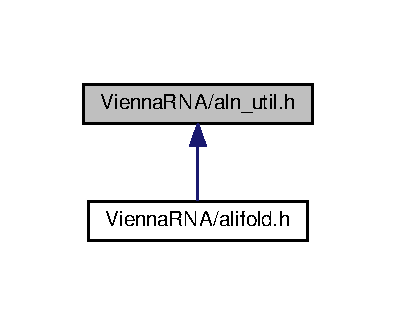
\includegraphics[width=190pt]{aln__util_8h__dep__incl}
\end{center}
\end{figure}
\subsection*{Data Structures}
\begin{DoxyCompactItemize}
\item 
struct \hyperlink{group__aln__utils_structvrna__pinfo__s}{vrna\+\_\+pinfo\+\_\+s}
\begin{DoxyCompactList}\small\item\em A base pair info structure.  \hyperlink{group__aln__utils_structvrna__pinfo__s}{More...}\end{DoxyCompactList}\end{DoxyCompactItemize}
\subsection*{Typedefs}
\begin{DoxyCompactItemize}
\item 
\hypertarget{group__aln__utils_ga6660dfca23debee7306e0cd53341263f}{typedef struct \hyperlink{group__aln__utils_structvrna__pinfo__s}{vrna\+\_\+pinfo\+\_\+s} \hyperlink{group__aln__utils_ga6660dfca23debee7306e0cd53341263f}{vrna\+\_\+pinfo\+\_\+t}}\label{group__aln__utils_ga6660dfca23debee7306e0cd53341263f}

\begin{DoxyCompactList}\small\item\em Typename for the base pair info repesenting data structure \hyperlink{group__aln__utils_structvrna__pinfo__s}{vrna\+\_\+pinfo\+\_\+s}. \end{DoxyCompactList}\item 
typedef struct \hyperlink{group__aln__utils_structvrna__pinfo__s}{vrna\+\_\+pinfo\+\_\+s} \hyperlink{group__aln__utils_ga7b61662a793ad0aa1ea38efc3a5baacc}{pair\+\_\+info}
\begin{DoxyCompactList}\small\item\em Old typename of \hyperlink{group__aln__utils_structvrna__pinfo__s}{vrna\+\_\+pinfo\+\_\+s}. \end{DoxyCompactList}\end{DoxyCompactItemize}
\subsection*{Functions}
\begin{DoxyCompactItemize}
\item 
int \hyperlink{group__consensus__fold_ga20fd17bb27891009af7ce839f5386177}{vrna\+\_\+aln\+\_\+mpi} (char $\ast$Alseq\mbox{[}$\,$\mbox{]}, int n\+\_\+seq, int length, int $\ast$mini)
\begin{DoxyCompactList}\small\item\em Get the mean pairwise identity in steps from ?to?(ident) \end{DoxyCompactList}\item 
\hyperlink{group__aln__utils_ga6660dfca23debee7306e0cd53341263f}{vrna\+\_\+pinfo\+\_\+t} $\ast$ \hyperlink{group__aln__utils_gaf6421a1318586c59fea6a127ed9f65f3}{vrna\+\_\+aln\+\_\+pinfo} (\hyperlink{group__fold__compound_ga1b0cef17fd40466cef5968eaeeff6166}{vrna\+\_\+fold\+\_\+compound\+\_\+t} $\ast$vc, const char $\ast$structure, double threshold)
\begin{DoxyCompactList}\small\item\em Retrieve an array of \hyperlink{group__aln__utils_ga6660dfca23debee7306e0cd53341263f}{vrna\+\_\+pinfo\+\_\+t} structures from precomputed pair probabilities. \end{DoxyCompactList}\item 
int \hyperlink{group__consensus__fold_gaa2d600be90844094ec145ea14a314d2f}{get\+\_\+mpi} (char $\ast$Alseq\mbox{[}$\,$\mbox{]}, int n\+\_\+seq, int length, int $\ast$mini)
\begin{DoxyCompactList}\small\item\em Get the mean pairwise identity in steps from ?to?(ident) \end{DoxyCompactList}\item 
void \hyperlink{group__consensus__fold_gaa3e40277c837d6f7603afe319884c786}{encode\+\_\+ali\+\_\+sequence} (const char $\ast$sequence, short $\ast$S, short $\ast$s5, short $\ast$s3, char $\ast$ss, unsigned short $\ast$as, int \hyperlink{group__model__details_gaf9202a1a09f5828dc731e2d9a10fa111}{circ})
\begin{DoxyCompactList}\small\item\em Get arrays with encoded sequence of the alignment. \end{DoxyCompactList}\item 
void \hyperlink{group__consensus__fold_ga8a560930f7f2582cc3967723a86cfdfa}{alloc\+\_\+sequence\+\_\+arrays} (const char $\ast$$\ast$sequences, short $\ast$$\ast$$\ast$S, short $\ast$$\ast$$\ast$S5, short $\ast$$\ast$$\ast$S3, unsigned short $\ast$$\ast$$\ast$a2s, char $\ast$$\ast$$\ast$Ss, int \hyperlink{group__model__details_gaf9202a1a09f5828dc731e2d9a10fa111}{circ})
\begin{DoxyCompactList}\small\item\em Allocate memory for sequence array used to deal with aligned sequences. \end{DoxyCompactList}\item 
void \hyperlink{group__consensus__fold_ga298a420a8c879202e2617b3f724fde38}{free\+\_\+sequence\+\_\+arrays} (unsigned int n\+\_\+seq, short $\ast$$\ast$$\ast$S, short $\ast$$\ast$$\ast$S5, short $\ast$$\ast$$\ast$S3, unsigned short $\ast$$\ast$$\ast$a2s, char $\ast$$\ast$$\ast$Ss)
\begin{DoxyCompactList}\small\item\em Free the memory of the sequence arrays used to deal with aligned sequences. \end{DoxyCompactList}\end{DoxyCompactItemize}


\subsection{Detailed Description}
Various utility-\/ and helper-\/functions for sequence alignments and comparative structure prediction. 


\input{boltzmann__sampling_8h}
\input{centroid_8h}
\input{cofold_8h}
\input{constraints_8h}
\input{convert__epars_8h}
\hypertarget{data__structures_8h}{\section{Vienna\+R\+N\+A/data\+\_\+structures.h File Reference}
\label{data__structures_8h}\index{Vienna\+R\+N\+A/data\+\_\+structures.\+h@{Vienna\+R\+N\+A/data\+\_\+structures.\+h}}
}
Include dependency graph for data\+\_\+structures.\+h\+:
\nopagebreak
\begin{figure}[H]
\begin{center}
\leavevmode
\includegraphics[width=350pt]{data__structures_8h__incl}
\end{center}
\end{figure}
This graph shows which files directly or indirectly include this file\+:
\nopagebreak
\begin{figure}[H]
\begin{center}
\leavevmode
\includegraphics[width=350pt]{data__structures_8h__dep__incl}
\end{center}
\end{figure}
\subsection*{Data Structures}
\begin{DoxyCompactItemize}
\item 
struct \hyperlink{group__data__structures_structvrna__basepair__s}{vrna\+\_\+basepair\+\_\+s}
\begin{DoxyCompactList}\small\item\em Base pair data structure used in subopt.\+c.  \hyperlink{group__data__structures_structvrna__basepair__s}{More...}\end{DoxyCompactList}\item 
struct \hyperlink{group__data__structures_structvrna__plist__s}{vrna\+\_\+plist\+\_\+s}
\begin{DoxyCompactList}\small\item\em this datastructure is used as input parameter in functions of \hyperlink{PS__dot_8h}{P\+S\+\_\+dot.\+h} and others  \hyperlink{group__data__structures_structvrna__plist__s}{More...}\end{DoxyCompactList}\item 
struct \hyperlink{group__data__structures_structvrna__cpair__s}{vrna\+\_\+cpair\+\_\+s}
\begin{DoxyCompactList}\small\item\em this datastructure is used as input parameter in functions of P\+S\+\_\+dot.\+c  \hyperlink{group__data__structures_structvrna__cpair__s}{More...}\end{DoxyCompactList}\item 
struct \hyperlink{group__data__structures_structvrna__sect__s}{vrna\+\_\+sect\+\_\+s}
\begin{DoxyCompactList}\small\item\em Stack of partial structures for backtracking.  \hyperlink{group__data__structures_structvrna__sect__s}{More...}\end{DoxyCompactList}\item 
struct \hyperlink{group__data__structures_structvrna__bp__stack__s}{vrna\+\_\+bp\+\_\+stack\+\_\+s}
\begin{DoxyCompactList}\small\item\em Base pair stack element.  \hyperlink{group__data__structures_structvrna__bp__stack__s}{More...}\end{DoxyCompactList}\item 
struct \hyperlink{group__data__structures_structpu__contrib}{pu\+\_\+contrib}
\begin{DoxyCompactList}\small\item\em contributions to p\+\_\+u  \hyperlink{group__data__structures_structpu__contrib}{More...}\end{DoxyCompactList}\item 
struct \hyperlink{group__data__structures_structinteract}{interact}
\item 
struct \hyperlink{group__data__structures_structpu__out}{pu\+\_\+out}
\begin{DoxyCompactList}\small\item\em Collection of all free\+\_\+energy of beeing unpaired values for output.  \hyperlink{group__data__structures_structpu__out}{More...}\end{DoxyCompactList}\item 
struct \hyperlink{group__data__structures_structconstrain}{constrain}
\begin{DoxyCompactList}\small\item\em constraints for cofolding  \hyperlink{group__data__structures_structconstrain}{More...}\end{DoxyCompactList}\item 
struct \hyperlink{group__data__structures_structduplexT}{duplex\+T}
\item 
struct \hyperlink{group__data__structures_structnode}{node}
\item 
struct \hyperlink{group__data__structures_structsnoopT}{snoop\+T}
\item 
struct \hyperlink{group__data__structures_structdupVar}{dup\+Var}
\item 
struct \hyperlink{group__fold__compound_structvrna__fc__s}{vrna\+\_\+fc\+\_\+s}
\begin{DoxyCompactList}\small\item\em The most basic data structure required by many functions throughout the R\+N\+Alib.  \hyperlink{group__fold__compound_structvrna__fc__s}{More...}\end{DoxyCompactList}\end{DoxyCompactItemize}
\subsection*{Macros}
\begin{DoxyCompactItemize}
\item 
\#define \hyperlink{group__fold__compound_ga1a5053dc8acbb0111e852988726f07d6}{V\+R\+N\+A\+\_\+\+S\+T\+A\+T\+U\+S\+\_\+\+M\+F\+E\+\_\+\+P\+R\+E}~(unsigned char)1
\begin{DoxyCompactList}\small\item\em Status message indicating that M\+F\+E computations are about to begin. \end{DoxyCompactList}\item 
\#define \hyperlink{group__fold__compound_ga47c900ca76e56e59e2e83a06e0bde641}{V\+R\+N\+A\+\_\+\+S\+T\+A\+T\+U\+S\+\_\+\+M\+F\+E\+\_\+\+P\+O\+S\+T}~(unsigned char)2
\begin{DoxyCompactList}\small\item\em Status message indicating that M\+F\+E computations are finished. \end{DoxyCompactList}\item 
\#define \hyperlink{group__fold__compound_ga91795d35ebdb6f32be50459f24b3d114}{V\+R\+N\+A\+\_\+\+S\+T\+A\+T\+U\+S\+\_\+\+P\+F\+\_\+\+P\+R\+E}~(unsigned char)3
\begin{DoxyCompactList}\small\item\em Status message indicating that Partition function computations are about to begin. \end{DoxyCompactList}\item 
\#define \hyperlink{group__fold__compound_ga1c6fa243533fd026e50f7d595eaaa565}{V\+R\+N\+A\+\_\+\+S\+T\+A\+T\+U\+S\+\_\+\+P\+F\+\_\+\+P\+O\+S\+T}~(unsigned char)4
\begin{DoxyCompactList}\small\item\em Status message indicating that Partition function computations are finished. \end{DoxyCompactList}\item 
\#define \hyperlink{group__fold__compound_gae63be9127fe7dcc1f9bb14f5bb1064ee}{V\+R\+N\+A\+\_\+\+O\+P\+T\+I\+O\+N\+\_\+\+M\+F\+E}~1
\begin{DoxyCompactList}\small\item\em Option flag to specify requirement of Minimum Free Energy (M\+F\+E) D\+P matrices and corresponding set of energy parameters. \end{DoxyCompactList}\item 
\#define \hyperlink{group__fold__compound_gabfbadcddda3e74ce7f49035ef8f058f7}{V\+R\+N\+A\+\_\+\+O\+P\+T\+I\+O\+N\+\_\+\+P\+F}~2
\begin{DoxyCompactList}\small\item\em Option flag to specify requirement of Partition Function (P\+F) D\+P matrices and corresponding set of Boltzmann factors. \end{DoxyCompactList}\item 
\#define \hyperlink{group__fold__compound_ga61469c423131552c8483229f8b6c7e0e}{V\+R\+N\+A\+\_\+\+O\+P\+T\+I\+O\+N\+\_\+\+E\+V\+A\+L\+\_\+\+O\+N\+L\+Y}~8
\begin{DoxyCompactList}\small\item\em Option flag to specify that neither M\+F\+E, nor P\+F D\+P matrices are required. \end{DoxyCompactList}\end{DoxyCompactItemize}
\subsection*{Typedefs}
\begin{DoxyCompactItemize}
\item 
\hypertarget{group__fold__compound_ga1b0cef17fd40466cef5968eaeeff6166}{typedef struct \hyperlink{group__fold__compound_structvrna__fc__s}{vrna\+\_\+fc\+\_\+s} \hyperlink{group__fold__compound_ga1b0cef17fd40466cef5968eaeeff6166}{vrna\+\_\+fold\+\_\+compound\+\_\+t}}\label{group__fold__compound_ga1b0cef17fd40466cef5968eaeeff6166}

\begin{DoxyCompactList}\small\item\em Typename for the fold\+\_\+compound data structure \hyperlink{group__fold__compound_structvrna__fc__s}{vrna\+\_\+fc\+\_\+s}. \end{DoxyCompactList}\item 
\hypertarget{group__data__structures_gac8c5669d3fb813cacf506489689305ce}{typedef struct \hyperlink{group__data__structures_structvrna__basepair__s}{vrna\+\_\+basepair\+\_\+s} \hyperlink{group__data__structures_gac8c5669d3fb813cacf506489689305ce}{vrna\+\_\+basepair\+\_\+t}}\label{group__data__structures_gac8c5669d3fb813cacf506489689305ce}

\begin{DoxyCompactList}\small\item\em Typename for the base pair repesenting data structure \hyperlink{group__data__structures_structvrna__basepair__s}{vrna\+\_\+basepair\+\_\+s}. \end{DoxyCompactList}\item 
\hypertarget{group__data__structures_ga8e4eb5e1bfc95776559575beb359af87}{typedef struct \hyperlink{group__data__structures_structvrna__plist__s}{vrna\+\_\+plist\+\_\+s} \hyperlink{group__data__structures_ga8e4eb5e1bfc95776559575beb359af87}{vrna\+\_\+plist\+\_\+t}}\label{group__data__structures_ga8e4eb5e1bfc95776559575beb359af87}

\begin{DoxyCompactList}\small\item\em Typename for the base pair list repesenting data structure \hyperlink{group__data__structures_structvrna__plist__s}{vrna\+\_\+plist\+\_\+s}. \end{DoxyCompactList}\item 
\hypertarget{group__data__structures_gaa651bda42e7692f08cb603cd6834b0ee}{typedef struct \hyperlink{group__data__structures_structvrna__bp__stack__s}{vrna\+\_\+bp\+\_\+stack\+\_\+s} \hyperlink{group__data__structures_gaa651bda42e7692f08cb603cd6834b0ee}{vrna\+\_\+bp\+\_\+stack\+\_\+t}}\label{group__data__structures_gaa651bda42e7692f08cb603cd6834b0ee}

\begin{DoxyCompactList}\small\item\em Typename for the base pair stack repesenting data structure \hyperlink{group__data__structures_structvrna__bp__stack__s}{vrna\+\_\+bp\+\_\+stack\+\_\+s}. \end{DoxyCompactList}\item 
\hypertarget{group__data__structures_gae4fc91141cc69c6d8eaf1332cb991ecc}{typedef struct \hyperlink{group__data__structures_structvrna__cpair__s}{vrna\+\_\+cpair\+\_\+s} \hyperlink{group__data__structures_gae4fc91141cc69c6d8eaf1332cb991ecc}{vrna\+\_\+cpair\+\_\+t}}\label{group__data__structures_gae4fc91141cc69c6d8eaf1332cb991ecc}

\begin{DoxyCompactList}\small\item\em Typename for data structure \hyperlink{group__data__structures_structvrna__cpair__s}{vrna\+\_\+cpair\+\_\+s}. \end{DoxyCompactList}\item 
\hypertarget{group__data__structures_gacc9cdae790dac75a7024e7069c0d4400}{typedef struct \hyperlink{group__data__structures_structvrna__sect__s}{vrna\+\_\+sect\+\_\+s} \hyperlink{group__data__structures_gacc9cdae790dac75a7024e7069c0d4400}{vrna\+\_\+sect\+\_\+t}}\label{group__data__structures_gacc9cdae790dac75a7024e7069c0d4400}

\begin{DoxyCompactList}\small\item\em Typename for stack of partial structures \hyperlink{group__data__structures_structvrna__sect__s}{vrna\+\_\+sect\+\_\+s}. \end{DoxyCompactList}\item 
\hypertarget{group__data__structures_ga31125aeace516926bf7f251f759b6126}{typedef double \hyperlink{group__data__structures_ga31125aeace516926bf7f251f759b6126}{F\+L\+T\+\_\+\+O\+R\+\_\+\+D\+B\+L}}\label{group__data__structures_ga31125aeace516926bf7f251f759b6126}

\begin{DoxyCompactList}\small\item\em Typename for floating point number in partition function computations. \end{DoxyCompactList}\item 
typedef void( \hyperlink{group__fold__compound_ga75aaf7b809290de808e545877a9e20f7}{vrna\+\_\+callback\+\_\+free\+\_\+auxdata} )(void $\ast$data)
\begin{DoxyCompactList}\small\item\em Callback to free memory allocated for auxiliary user-\/provided data. \end{DoxyCompactList}\item 
typedef void( \hyperlink{group__fold__compound_ga9fafb3f0217e27339bb9faf61a03e723}{vrna\+\_\+callback\+\_\+recursion\+\_\+status} )(\hyperlink{group__fold__compound_ga1b0cef17fd40466cef5968eaeeff6166}{vrna\+\_\+fold\+\_\+compound\+\_\+t} $\ast$vc, unsigned char status)
\begin{DoxyCompactList}\small\item\em Callback to perform specific user-\/defined actions before, or after recursive computations. \end{DoxyCompactList}\item 
typedef struct \hyperlink{group__data__structures_structvrna__basepair__s}{vrna\+\_\+basepair\+\_\+s} \hyperlink{group__data__structures_ga4381025ffbd692e54189b2c679c79c99}{P\+A\+I\+R}
\begin{DoxyCompactList}\small\item\em Old typename of \hyperlink{group__data__structures_structvrna__basepair__s}{vrna\+\_\+basepair\+\_\+s}. \end{DoxyCompactList}\item 
typedef struct \hyperlink{group__data__structures_structvrna__plist__s}{vrna\+\_\+plist\+\_\+s} \hyperlink{group__data__structures_gab1d8894b43aa84cbc50b862a73785fbc}{plist}
\begin{DoxyCompactList}\small\item\em Old typename of \hyperlink{group__data__structures_structvrna__plist__s}{vrna\+\_\+plist\+\_\+s}. \end{DoxyCompactList}\item 
typedef struct \hyperlink{group__data__structures_structvrna__cpair__s}{vrna\+\_\+cpair\+\_\+s} \hyperlink{group__data__structures_ga8412f116a2eb07b59ade9e14ca7c5ef1}{cpair}
\begin{DoxyCompactList}\small\item\em Old typename of \hyperlink{group__data__structures_structvrna__cpair__s}{vrna\+\_\+cpair\+\_\+s}. \end{DoxyCompactList}\item 
typedef struct \hyperlink{group__data__structures_structvrna__sect__s}{vrna\+\_\+sect\+\_\+s} \hyperlink{group__data__structures_gaaacedee1f05d3d45aa6764eca51a8876}{sect}
\begin{DoxyCompactList}\small\item\em Old typename of \hyperlink{group__data__structures_structvrna__sect__s}{vrna\+\_\+sect\+\_\+s}. \end{DoxyCompactList}\item 
typedef struct \hyperlink{group__data__structures_structvrna__bp__stack__s}{vrna\+\_\+bp\+\_\+stack\+\_\+s} \hyperlink{group__data__structures_gaaeed53a7508c6ce549a98223e94b25df}{bond\+T}
\begin{DoxyCompactList}\small\item\em Old typename of \hyperlink{group__data__structures_structvrna__bp__stack__s}{vrna\+\_\+bp\+\_\+stack\+\_\+s}. \end{DoxyCompactList}\item 
\hypertarget{group__data__structures_ga20881ac02e5932356c09b070efedb560}{typedef struct \hyperlink{group__data__structures_structpu__contrib}{pu\+\_\+contrib} \hyperlink{group__data__structures_ga20881ac02e5932356c09b070efedb560}{pu\+\_\+contrib}}\label{group__data__structures_ga20881ac02e5932356c09b070efedb560}

\begin{DoxyCompactList}\small\item\em contributions to p\+\_\+u \end{DoxyCompactList}\item 
\hypertarget{group__data__structures_ga501763bd204b60f40e3ab68b40023023}{typedef struct \hyperlink{group__data__structures_structpu__out}{pu\+\_\+out} \hyperlink{group__data__structures_ga501763bd204b60f40e3ab68b40023023}{pu\+\_\+out}}\label{group__data__structures_ga501763bd204b60f40e3ab68b40023023}

\begin{DoxyCompactList}\small\item\em Collection of all free\+\_\+energy of beeing unpaired values for output. \end{DoxyCompactList}\item 
\hypertarget{group__data__structures_ga212e3afb0cc299acdfb1ec976435686e}{typedef struct \hyperlink{group__data__structures_structconstrain}{constrain} \hyperlink{group__data__structures_ga212e3afb0cc299acdfb1ec976435686e}{constrain}}\label{group__data__structures_ga212e3afb0cc299acdfb1ec976435686e}

\begin{DoxyCompactList}\small\item\em constraints for cofolding \end{DoxyCompactList}\end{DoxyCompactItemize}
\subsection*{Enumerations}
\begin{DoxyCompactItemize}
\item 
enum \hyperlink{group__fold__compound_ga01a4ff86fa71deaaa5d1abbd95a1447d}{vrna\+\_\+fc\+\_\+type\+\_\+e} \{ \hyperlink{group__fold__compound_gga01a4ff86fa71deaaa5d1abbd95a1447da1608d3aa78905fc39e0d25a624ac9512}{V\+R\+N\+A\+\_\+\+V\+C\+\_\+\+T\+Y\+P\+E\+\_\+\+S\+I\+N\+G\+L\+E}, 
\hyperlink{group__fold__compound_gga01a4ff86fa71deaaa5d1abbd95a1447da056345f1bcfe7cd595d1fd437c05246d}{V\+R\+N\+A\+\_\+\+V\+C\+\_\+\+T\+Y\+P\+E\+\_\+\+A\+L\+I\+G\+N\+M\+E\+N\+T}
 \}
\begin{DoxyCompactList}\small\item\em An enumerator that is used to specify the type of a \hyperlink{group__fold__compound_ga1b0cef17fd40466cef5968eaeeff6166}{vrna\+\_\+fold\+\_\+compound\+\_\+t}. \end{DoxyCompactList}\end{DoxyCompactItemize}
\subsection*{Functions}
\begin{DoxyCompactItemize}
\item 
\hyperlink{group__fold__compound_ga1b0cef17fd40466cef5968eaeeff6166}{vrna\+\_\+fold\+\_\+compound\+\_\+t} $\ast$ \hyperlink{group__fold__compound_ga6601d994ba32b11511b36f68b08403be}{vrna\+\_\+fold\+\_\+compound} (const char $\ast$sequence, \hyperlink{group__model__details_ga1f8a10e12a0a1915f2a4eff0b28ea17c}{vrna\+\_\+md\+\_\+t} $\ast$md\+\_\+p, unsigned int options)
\begin{DoxyCompactList}\small\item\em Retrieve a \hyperlink{group__fold__compound_ga1b0cef17fd40466cef5968eaeeff6166}{vrna\+\_\+fold\+\_\+compound\+\_\+t} data structure for single sequences and hybridizing sequences. \end{DoxyCompactList}\item 
\hyperlink{group__fold__compound_ga1b0cef17fd40466cef5968eaeeff6166}{vrna\+\_\+fold\+\_\+compound\+\_\+t} $\ast$ \hyperlink{group__fold__compound_gad6bacc816af274922b13d947f708aa0c}{vrna\+\_\+fold\+\_\+compound\+\_\+comparative} (const char $\ast$$\ast$sequences, \hyperlink{group__model__details_ga1f8a10e12a0a1915f2a4eff0b28ea17c}{vrna\+\_\+md\+\_\+t} $\ast$md\+\_\+p, unsigned int options)
\begin{DoxyCompactList}\small\item\em Retrieve a \hyperlink{group__fold__compound_ga1b0cef17fd40466cef5968eaeeff6166}{vrna\+\_\+fold\+\_\+compound\+\_\+t} data structure for sequence alignments. \end{DoxyCompactList}\item 
void \hyperlink{group__fold__compound_gadded6039d63f5d6509836e20321534ad}{vrna\+\_\+fold\+\_\+compound\+\_\+free} (\hyperlink{group__fold__compound_ga1b0cef17fd40466cef5968eaeeff6166}{vrna\+\_\+fold\+\_\+compound\+\_\+t} $\ast$vc)
\begin{DoxyCompactList}\small\item\em Free memory occupied by a \hyperlink{group__fold__compound_ga1b0cef17fd40466cef5968eaeeff6166}{vrna\+\_\+fold\+\_\+compound\+\_\+t}. \end{DoxyCompactList}\item 
void \hyperlink{group__fold__compound_ga6316a9426bea2f742375e8df6febd3f6}{vrna\+\_\+fold\+\_\+compound\+\_\+add\+\_\+auxdata} (\hyperlink{group__fold__compound_ga1b0cef17fd40466cef5968eaeeff6166}{vrna\+\_\+fold\+\_\+compound\+\_\+t} $\ast$vc, void $\ast$data, \hyperlink{group__fold__compound_ga75aaf7b809290de808e545877a9e20f7}{vrna\+\_\+callback\+\_\+free\+\_\+auxdata} $\ast$f)
\begin{DoxyCompactList}\small\item\em Add auxiliary data to the \hyperlink{group__fold__compound_ga1b0cef17fd40466cef5968eaeeff6166}{vrna\+\_\+fold\+\_\+compound\+\_\+t}. \end{DoxyCompactList}\item 
void \hyperlink{group__fold__compound_ga097ed6133055624667cbce8cfdebf82d}{vrna\+\_\+fold\+\_\+compound\+\_\+add\+\_\+callback} (\hyperlink{group__fold__compound_ga1b0cef17fd40466cef5968eaeeff6166}{vrna\+\_\+fold\+\_\+compound\+\_\+t} $\ast$vc, \hyperlink{group__fold__compound_ga9fafb3f0217e27339bb9faf61a03e723}{vrna\+\_\+callback\+\_\+recursion\+\_\+status} $\ast$f)
\begin{DoxyCompactList}\small\item\em Add a recursion status callback to the \hyperlink{group__fold__compound_ga1b0cef17fd40466cef5968eaeeff6166}{vrna\+\_\+fold\+\_\+compound\+\_\+t}. \end{DoxyCompactList}\end{DoxyCompactItemize}

\input{dist__vars_8h}
\hypertarget{dp__matrices_8h}{\section{Vienna\+R\+N\+A/dp\+\_\+matrices.h File Reference}
\label{dp__matrices_8h}\index{Vienna\+R\+N\+A/dp\+\_\+matrices.\+h@{Vienna\+R\+N\+A/dp\+\_\+matrices.\+h}}
}
Include dependency graph for dp\+\_\+matrices.\+h\+:
\nopagebreak
\begin{figure}[H]
\begin{center}
\leavevmode
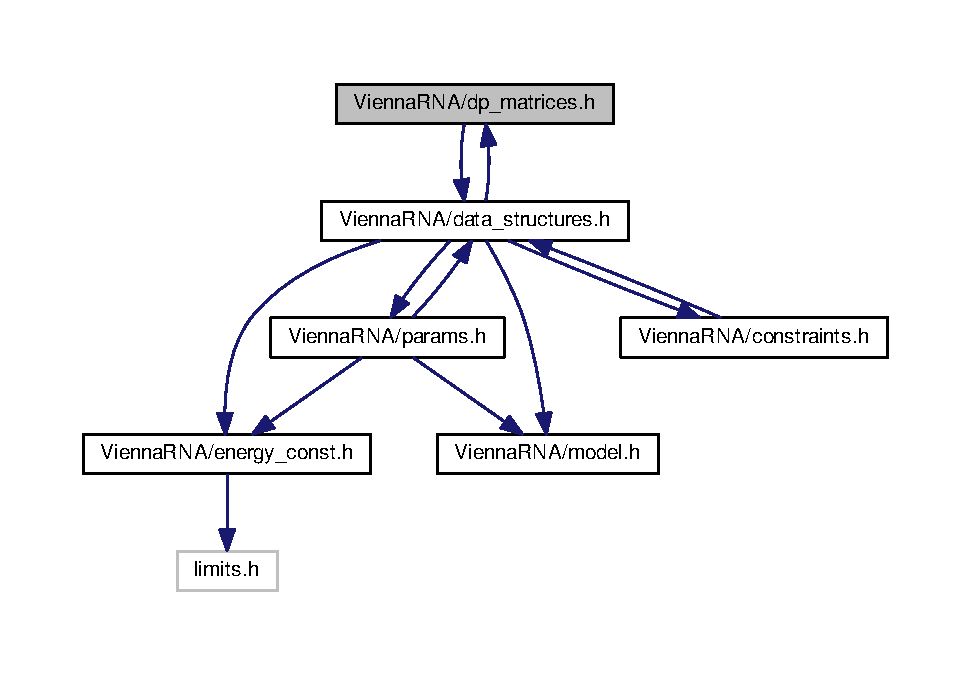
\includegraphics[width=350pt]{dp__matrices_8h__incl}
\end{center}
\end{figure}
This graph shows which files directly or indirectly include this file\+:
\nopagebreak
\begin{figure}[H]
\begin{center}
\leavevmode
\includegraphics[width=350pt]{dp__matrices_8h__dep__incl}
\end{center}
\end{figure}
\subsection*{Data Structures}
\begin{DoxyCompactItemize}
\item 
struct \hyperlink{group__dp__matrices_structvrna__mx__mfe__s}{vrna\+\_\+mx\+\_\+mfe\+\_\+s}
\begin{DoxyCompactList}\small\item\em Minimum Free Energy (M\+F\+E) Dynamic Programming (D\+P) matrices data structure required within the \hyperlink{group__fold__compound_ga1b0cef17fd40466cef5968eaeeff6166}{vrna\+\_\+fold\+\_\+compound\+\_\+t}.  \hyperlink{group__dp__matrices_structvrna__mx__mfe__s}{More...}\end{DoxyCompactList}\item 
struct \hyperlink{group__dp__matrices_structvrna__mx__pf__s}{vrna\+\_\+mx\+\_\+pf\+\_\+s}
\begin{DoxyCompactList}\small\item\em Partition function (P\+F) Dynamic Programming (D\+P) matrices data structure required within the \hyperlink{group__fold__compound_ga1b0cef17fd40466cef5968eaeeff6166}{vrna\+\_\+fold\+\_\+compound\+\_\+t}.  \hyperlink{group__dp__matrices_structvrna__mx__pf__s}{More...}\end{DoxyCompactList}\end{DoxyCompactItemize}
\subsection*{Typedefs}
\begin{DoxyCompactItemize}
\item 
\hypertarget{group__dp__matrices_gae5aef35d016475e758f619b7bcb534f9}{typedef struct \hyperlink{group__dp__matrices_structvrna__mx__mfe__s}{vrna\+\_\+mx\+\_\+mfe\+\_\+s} \hyperlink{group__dp__matrices_gae5aef35d016475e758f619b7bcb534f9}{vrna\+\_\+mx\+\_\+mfe\+\_\+t}}\label{group__dp__matrices_gae5aef35d016475e758f619b7bcb534f9}

\begin{DoxyCompactList}\small\item\em Typename for the Minimum Free Energy (M\+F\+E) D\+P matrices data structure \hyperlink{group__dp__matrices_structvrna__mx__mfe__s}{vrna\+\_\+mx\+\_\+mfe\+\_\+s}. \end{DoxyCompactList}\item 
\hypertarget{group__dp__matrices_ga68729ab3fed26bdd1806fa814f172fc1}{typedef struct \hyperlink{group__dp__matrices_structvrna__mx__pf__s}{vrna\+\_\+mx\+\_\+pf\+\_\+s} \hyperlink{group__dp__matrices_ga68729ab3fed26bdd1806fa814f172fc1}{vrna\+\_\+mx\+\_\+pf\+\_\+t}}\label{group__dp__matrices_ga68729ab3fed26bdd1806fa814f172fc1}

\begin{DoxyCompactList}\small\item\em Typename for the Partition Function (P\+F) D\+P matrices data structure \hyperlink{group__dp__matrices_structvrna__mx__pf__s}{vrna\+\_\+mx\+\_\+pf\+\_\+s}. \end{DoxyCompactList}\end{DoxyCompactItemize}
\subsection*{Enumerations}
\begin{DoxyCompactItemize}
\item 
enum \hyperlink{group__dp__matrices_ga6042ea1d58d01931e959791be6d89343}{vrna\+\_\+mx\+\_\+type\+\_\+e} \{ \hyperlink{group__dp__matrices_gga6042ea1d58d01931e959791be6d89343aafa2568956dab79595521e20c49a5f75}{V\+R\+N\+A\+\_\+\+M\+X\+\_\+\+D\+E\+F\+A\+U\+L\+T}, 
\hyperlink{group__dp__matrices_gga6042ea1d58d01931e959791be6d89343a2ea5d5947f6ec02544934b0ff2785e99}{V\+R\+N\+A\+\_\+\+M\+X\+\_\+\+W\+I\+N\+D\+O\+W}, 
\hyperlink{group__dp__matrices_gga6042ea1d58d01931e959791be6d89343ae656f8391445ff71bed8a597a0a19417}{V\+R\+N\+A\+\_\+\+M\+X\+\_\+2\+D\+F\+O\+L\+D}
 \}
\begin{DoxyCompactList}\small\item\em An enumerator that is used to specify the type of a polymorphic Dynamic Programming (D\+P) matrix data structure. \end{DoxyCompactList}\end{DoxyCompactItemize}
\subsection*{Functions}
\begin{DoxyCompactItemize}
\item 
int \hyperlink{group__dp__matrices_ga08661f098008961dab0023bf300f0c33}{vrna\+\_\+mx\+\_\+add} (\hyperlink{group__fold__compound_ga1b0cef17fd40466cef5968eaeeff6166}{vrna\+\_\+fold\+\_\+compound\+\_\+t} $\ast$vc, \hyperlink{group__dp__matrices_ga6042ea1d58d01931e959791be6d89343}{vrna\+\_\+mx\+\_\+type\+\_\+e} type, unsigned int options)
\begin{DoxyCompactList}\small\item\em Add Dynamic Programming (D\+P) matrices (allocate memory) \end{DoxyCompactList}\item 
void \hyperlink{group__dp__matrices_ga6a9422feb5dfe5c64050cebf447672d0}{vrna\+\_\+mx\+\_\+mfe\+\_\+free} (\hyperlink{group__fold__compound_ga1b0cef17fd40466cef5968eaeeff6166}{vrna\+\_\+fold\+\_\+compound\+\_\+t} $\ast$vc)
\begin{DoxyCompactList}\small\item\em Free memory occupied by the Minimum Free Energy (M\+F\+E) Dynamic Programming (D\+P) matrices. \end{DoxyCompactList}\item 
void \hyperlink{group__dp__matrices_ga2283e69fd139fb8e58d7ade3b5773f9c}{vrna\+\_\+mx\+\_\+pf\+\_\+free} (\hyperlink{group__fold__compound_ga1b0cef17fd40466cef5968eaeeff6166}{vrna\+\_\+fold\+\_\+compound\+\_\+t} $\ast$vc)
\begin{DoxyCompactList}\small\item\em Free memory occupied by the Partition Function (P\+F) Dynamic Programming (D\+P) matrices. \end{DoxyCompactList}\end{DoxyCompactItemize}

\hypertarget{duplex_8h}{}\section{Vienna\+R\+N\+A/duplex.h File Reference}
\label{duplex_8h}\index{Vienna\+R\+N\+A/duplex.\+h@{Vienna\+R\+N\+A/duplex.\+h}}


Duplex folding function declarations...  


Include dependency graph for duplex.\+h\+:
\nopagebreak
\begin{figure}[H]
\begin{center}
\leavevmode
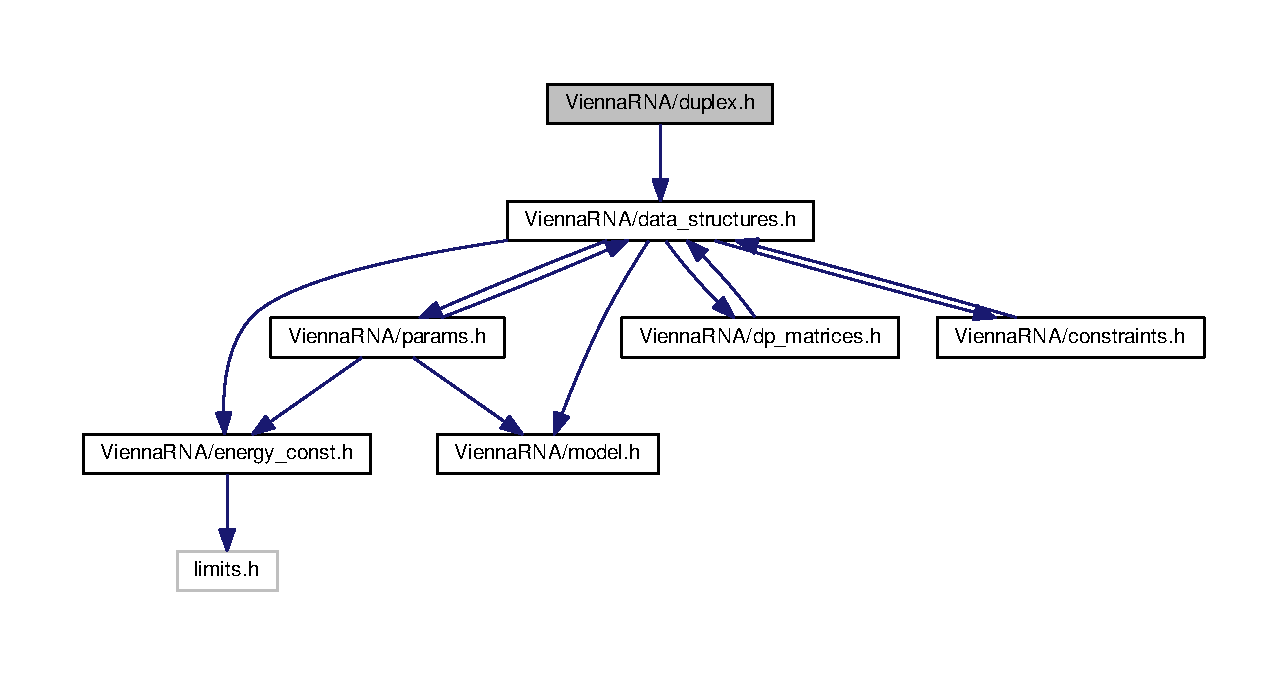
\includegraphics[width=350pt]{duplex_8h__incl}
\end{center}
\end{figure}


\subsection{Detailed Description}
Duplex folding function declarations... 


\input{edit__cost_8h}
\input{energy__const_8h}
\hypertarget{eval_8h}{}\section{Vienna\+R\+N\+A/eval.h File Reference}
\label{eval_8h}\index{Vienna\+R\+N\+A/eval.\+h@{Vienna\+R\+N\+A/eval.\+h}}


Functions and variables related to energy evaluation of sequence/structure pairs.  


Include dependency graph for eval.\+h\+:
\nopagebreak
\begin{figure}[H]
\begin{center}
\leavevmode
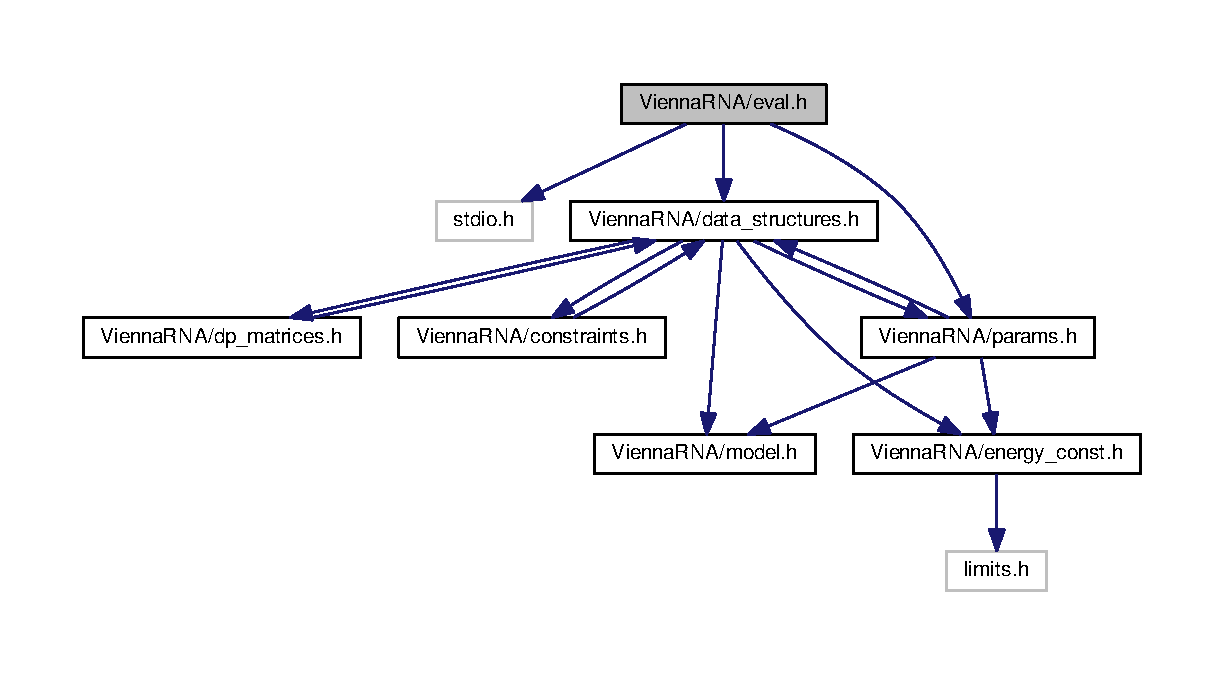
\includegraphics[width=350pt]{eval_8h__incl}
\end{center}
\end{figure}
This graph shows which files directly or indirectly include this file\+:
\nopagebreak
\begin{figure}[H]
\begin{center}
\leavevmode
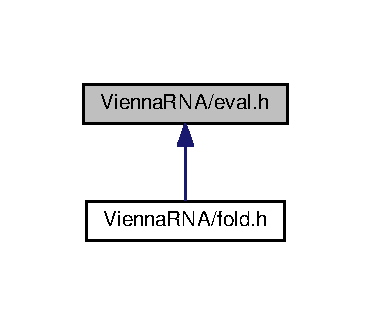
\includegraphics[width=178pt]{eval_8h__dep__incl}
\end{center}
\end{figure}
\subsection*{Functions}
\begin{DoxyCompactItemize}
\item 
float \hyperlink{group__eval_ga58f199f1438d794a265f3b27fc8ea631}{vrna\+\_\+eval\+\_\+structure} (\hyperlink{group__fold__compound_ga1b0cef17fd40466cef5968eaeeff6166}{vrna\+\_\+fold\+\_\+compound\+\_\+t} $\ast$vc, const char $\ast$structure)
\begin{DoxyCompactList}\small\item\em Calculate the free energy of an already folded R\+N\+A. \end{DoxyCompactList}\item 
float \hyperlink{group__eval_ga6cea75c0eb9857fb59172be54cab09e0}{vrna\+\_\+eval\+\_\+covar\+\_\+structure} (\hyperlink{group__fold__compound_ga1b0cef17fd40466cef5968eaeeff6166}{vrna\+\_\+fold\+\_\+compound\+\_\+t} $\ast$vc, const char $\ast$structure)
\begin{DoxyCompactList}\small\item\em Calculate the pseudo energy derived by the covariance scores of a set of aligned sequences. \end{DoxyCompactList}\item 
float \hyperlink{group__eval_gab6930f446d04761454d033680fbf7909}{vrna\+\_\+eval\+\_\+structure\+\_\+simple} (const char $\ast$string, const char $\ast$structure)
\begin{DoxyCompactList}\small\item\em Calculate the free energy of an already folded R\+N\+A. \end{DoxyCompactList}\item 
float \hyperlink{group__eval_ga0928d699d310178f84ee2351034e5cb5}{vrna\+\_\+eval\+\_\+structure\+\_\+verbose} (\hyperlink{group__fold__compound_ga1b0cef17fd40466cef5968eaeeff6166}{vrna\+\_\+fold\+\_\+compound\+\_\+t} $\ast$vc, const char $\ast$structure, F\+I\+L\+E $\ast$file)
\begin{DoxyCompactList}\small\item\em Calculate the free energy of an already folded R\+N\+A and print contributions on a per-\/loop base. \end{DoxyCompactList}\item 
float \hyperlink{group__eval_ga4c2895a7dcd756ef2dc7f76db7c4c53e}{vrna\+\_\+eval\+\_\+structure\+\_\+simple\+\_\+verbose} (const char $\ast$string, const char $\ast$structure, F\+I\+L\+E $\ast$file)
\begin{DoxyCompactList}\small\item\em Calculate the free energy of an already folded R\+N\+A and print contributions per loop. \end{DoxyCompactList}\item 
int \hyperlink{group__eval_gadbd09372ddfd7a450bbd590c96a6bfe4}{vrna\+\_\+eval\+\_\+structure\+\_\+pt} (\hyperlink{group__fold__compound_ga1b0cef17fd40466cef5968eaeeff6166}{vrna\+\_\+fold\+\_\+compound\+\_\+t} $\ast$vc, const short $\ast$pt)
\begin{DoxyCompactList}\small\item\em Calculate the free energy of an already folded R\+N\+A. \end{DoxyCompactList}\item 
int \hyperlink{group__eval_ga0bba59b4d6e53461088666ff4aece7b0}{vrna\+\_\+eval\+\_\+structure\+\_\+pt\+\_\+simple} (const char $\ast$string, const short $\ast$pt)
\begin{DoxyCompactList}\small\item\em Calculate the free energy of an already folded R\+N\+A. \end{DoxyCompactList}\item 
int \hyperlink{group__eval_ga8a517cfeeae8c376ae7b1e0c401d38b4}{vrna\+\_\+eval\+\_\+structure\+\_\+pt\+\_\+verbose} (\hyperlink{group__fold__compound_ga1b0cef17fd40466cef5968eaeeff6166}{vrna\+\_\+fold\+\_\+compound\+\_\+t} $\ast$vc, const short $\ast$pt, F\+I\+L\+E $\ast$file)
\begin{DoxyCompactList}\small\item\em Calculate the free energy of an already folded R\+N\+A. \end{DoxyCompactList}\item 
int \hyperlink{group__eval_ga76e152ee9a02be23da14cdddf52b4e44}{vrna\+\_\+eval\+\_\+structure\+\_\+pt\+\_\+simple\+\_\+verbose} (const char $\ast$string, const short $\ast$pt, F\+I\+L\+E $\ast$file)
\begin{DoxyCompactList}\small\item\em Calculate the free energy of an already folded R\+N\+A. \end{DoxyCompactList}\item 
int \hyperlink{group__eval_ga730ba4df55c02fd530a0cddd49faf760}{vrna\+\_\+eval\+\_\+loop\+\_\+pt} (\hyperlink{group__fold__compound_ga1b0cef17fd40466cef5968eaeeff6166}{vrna\+\_\+fold\+\_\+compound\+\_\+t} $\ast$vc, int i, const short $\ast$pt)
\begin{DoxyCompactList}\small\item\em Calculate energy of a loop. \end{DoxyCompactList}\item 
float \hyperlink{group__eval_gaff1b9e4f4d17b434b0a822fe783672c1}{vrna\+\_\+eval\+\_\+move} (\hyperlink{group__fold__compound_ga1b0cef17fd40466cef5968eaeeff6166}{vrna\+\_\+fold\+\_\+compound\+\_\+t} $\ast$vc, const char $\ast$structure, int m1, int m2)
\begin{DoxyCompactList}\small\item\em Calculate energy of a move (closing or opening of a base pair) \end{DoxyCompactList}\item 
int \hyperlink{group__eval_ga123dabc119ea98c968a5e903cc46f0fb}{vrna\+\_\+eval\+\_\+move\+\_\+pt} (\hyperlink{group__fold__compound_ga1b0cef17fd40466cef5968eaeeff6166}{vrna\+\_\+fold\+\_\+compound\+\_\+t} $\ast$vc, short $\ast$pt, int m1, int m2)
\begin{DoxyCompactList}\small\item\em Calculate energy of a move (closing or opening of a base pair) \end{DoxyCompactList}\item 
float \hyperlink{group__eval_gaf93986cb3cb29770ec9cca69c9fab8cf}{energy\+\_\+of\+\_\+structure} (const char $\ast$string, const char $\ast$structure, int verbosity\+\_\+level)
\begin{DoxyCompactList}\small\item\em Calculate the free energy of an already folded R\+N\+A using global model detail settings. \end{DoxyCompactList}\item 
float \hyperlink{group__eval_gaf9d064d3c496de42eca6734a96fd2090}{energy\+\_\+of\+\_\+struct\+\_\+par} (const char $\ast$string, const char $\ast$structure, \hyperlink{group__energy__parameters_ga8a69ca7d787e4fd6079914f5343a1f35}{vrna\+\_\+param\+\_\+t} $\ast$parameters, int verbosity\+\_\+level)
\begin{DoxyCompactList}\small\item\em Calculate the free energy of an already folded R\+N\+A. \end{DoxyCompactList}\item 
float \hyperlink{group__eval_gaeb14f3664aec67fc03268ac75253f0f8}{energy\+\_\+of\+\_\+circ\+\_\+structure} (const char $\ast$string, const char $\ast$structure, int verbosity\+\_\+level)
\begin{DoxyCompactList}\small\item\em Calculate the free energy of an already folded circular R\+N\+A. \end{DoxyCompactList}\item 
float \hyperlink{group__eval_ga3f01f9744ba6a40555eb4d81fc77f6df}{energy\+\_\+of\+\_\+circ\+\_\+struct\+\_\+par} (const char $\ast$string, const char $\ast$structure, \hyperlink{group__energy__parameters_ga8a69ca7d787e4fd6079914f5343a1f35}{vrna\+\_\+param\+\_\+t} $\ast$parameters, int verbosity\+\_\+level)
\begin{DoxyCompactList}\small\item\em Calculate the free energy of an already folded circular R\+N\+A. \end{DoxyCompactList}\item 
int \hyperlink{group__eval_ga8831445966b761417e713360791299d8}{energy\+\_\+of\+\_\+structure\+\_\+pt} (const char $\ast$string, short $\ast$ptable, short $\ast$s, short $\ast$s1, int verbosity\+\_\+level)
\begin{DoxyCompactList}\small\item\em Calculate the free energy of an already folded R\+N\+A. \end{DoxyCompactList}\item 
int \hyperlink{group__eval_ga49acb3d5627dc6823a7ce12d116d4c69}{energy\+\_\+of\+\_\+struct\+\_\+pt\+\_\+par} (const char $\ast$string, short $\ast$ptable, short $\ast$s, short $\ast$s1, \hyperlink{group__energy__parameters_ga8a69ca7d787e4fd6079914f5343a1f35}{vrna\+\_\+param\+\_\+t} $\ast$parameters, int verbosity\+\_\+level)
\begin{DoxyCompactList}\small\item\em Calculate the free energy of an already folded R\+N\+A. \end{DoxyCompactList}\item 
float \hyperlink{group__eval_ga539ecaed89730f7644c202f304d7529b}{energy\+\_\+of\+\_\+move} (const char $\ast$string, const char $\ast$structure, int m1, int m2)
\begin{DoxyCompactList}\small\item\em Calculate energy of a move (closing or opening of a base pair) \end{DoxyCompactList}\item 
int \hyperlink{group__eval_ga49e0ee561be69faf0568213546f6a53f}{energy\+\_\+of\+\_\+move\+\_\+pt} (short $\ast$pt, short $\ast$s, short $\ast$s1, int m1, int m2)
\begin{DoxyCompactList}\small\item\em Calculate energy of a move (closing or opening of a base pair) \end{DoxyCompactList}\item 
int \hyperlink{group__eval_ga507d4fd93f4b398d793ba2402731388d}{loop\+\_\+energy} (short $\ast$ptable, short $\ast$s, short $\ast$s1, int i)
\begin{DoxyCompactList}\small\item\em Calculate energy of a loop. \end{DoxyCompactList}\item 
float \hyperlink{group__eval_gac2b37fea2145c94d925a3f33378ef87b}{energy\+\_\+of\+\_\+struct} (const char $\ast$string, const char $\ast$structure)
\item 
int \hyperlink{group__eval_ga27ce6f68512d43bf1fe14a06c9d76d5c}{energy\+\_\+of\+\_\+struct\+\_\+pt} (const char $\ast$string, short $\ast$ptable, short $\ast$s, short $\ast$s1)
\item 
float \hyperlink{group__eval_ga657222e2758c46bf13b416ef3032e417}{energy\+\_\+of\+\_\+circ\+\_\+struct} (const char $\ast$string, const char $\ast$structure)
\end{DoxyCompactItemize}
\subsection*{Variables}
\begin{DoxyCompactItemize}
\item 
\hypertarget{group__eval_gab9b2c3a37a5516614c06d0ab54b97cda}{}int \hyperlink{group__eval_gab9b2c3a37a5516614c06d0ab54b97cda}{cut\+\_\+point}\label{group__eval_gab9b2c3a37a5516614c06d0ab54b97cda}

\begin{DoxyCompactList}\small\item\em set to first pos of second seq for cofolding \end{DoxyCompactList}\item 
\hypertarget{group__eval_ga567530678f6260a1a649a5beca5da4c5}{}int \hyperlink{group__eval_ga567530678f6260a1a649a5beca5da4c5}{eos\+\_\+debug}\label{group__eval_ga567530678f6260a1a649a5beca5da4c5}

\begin{DoxyCompactList}\small\item\em verbose info from energy\+\_\+of\+\_\+struct \end{DoxyCompactList}\end{DoxyCompactItemize}


\subsection{Detailed Description}
Functions and variables related to energy evaluation of sequence/structure pairs. 


\input{exterior__loops_8h}
\input{file__formats_8h}
\hypertarget{findpath_8h}{}\section{Vienna\+R\+N\+A/findpath.h File Reference}
\label{findpath_8h}\index{Vienna\+R\+N\+A/findpath.\+h@{Vienna\+R\+N\+A/findpath.\+h}}
Include dependency graph for findpath.\+h\+:
\nopagebreak
\begin{figure}[H]
\begin{center}
\leavevmode
\includegraphics[width=350pt]{findpath_8h__incl}
\end{center}
\end{figure}
\subsection*{Data Structures}
\begin{DoxyCompactItemize}
\item 
struct \hyperlink{group__direct__paths_structvrna__path__s}{vrna\+\_\+path\+\_\+s}
\begin{DoxyCompactList}\small\item\em An element of a refolding path list.  \hyperlink{group__direct__paths_structvrna__path__s}{More...}\end{DoxyCompactList}\end{DoxyCompactItemize}
\subsection*{Typedefs}
\begin{DoxyCompactItemize}
\item 
\hypertarget{group__direct__paths_ga818d4f3d1cf8723d6905990b08d909fe}{}typedef struct \hyperlink{group__direct__paths_structvrna__path__s}{vrna\+\_\+path\+\_\+s} \hyperlink{group__direct__paths_ga818d4f3d1cf8723d6905990b08d909fe}{vrna\+\_\+path\+\_\+t}\label{group__direct__paths_ga818d4f3d1cf8723d6905990b08d909fe}

\begin{DoxyCompactList}\small\item\em Typename for the refolding path data structure \hyperlink{group__direct__paths_structvrna__path__s}{vrna\+\_\+path\+\_\+s}. \end{DoxyCompactList}\item 
typedef struct \hyperlink{group__direct__paths_structvrna__path__s}{vrna\+\_\+path\+\_\+s} \hyperlink{group__direct__paths_gab6b8737d5377e70a7815d04aae7fd884}{path\+\_\+t}
\begin{DoxyCompactList}\small\item\em Old typename of \hyperlink{group__direct__paths_structvrna__path__s}{vrna\+\_\+path\+\_\+s}. \end{DoxyCompactList}\end{DoxyCompactItemize}
\subsection*{Functions}
\begin{DoxyCompactItemize}
\item 
int \hyperlink{group__direct__paths_ga957922acc1bcaa97f52cbd0975f7dcd0}{vrna\+\_\+path\+\_\+findpath\+\_\+saddle} (\hyperlink{group__fold__compound_ga1b0cef17fd40466cef5968eaeeff6166}{vrna\+\_\+fold\+\_\+compound\+\_\+t} $\ast$vc, const char $\ast$struc1, const char $\ast$struc2, int max)
\begin{DoxyCompactList}\small\item\em Find energy of a saddle point between 2 structures (search only direct path) \end{DoxyCompactList}\item 
\hyperlink{group__direct__paths_ga818d4f3d1cf8723d6905990b08d909fe}{vrna\+\_\+path\+\_\+t} $\ast$ \hyperlink{group__direct__paths_ga5e1f97f58adc65016a8df88802dc16b5}{vrna\+\_\+path\+\_\+findpath} (\hyperlink{group__fold__compound_ga1b0cef17fd40466cef5968eaeeff6166}{vrna\+\_\+fold\+\_\+compound\+\_\+t} $\ast$vc, const char $\ast$s1, const char $\ast$s2, int maxkeep)
\begin{DoxyCompactList}\small\item\em Find refolding path between 2 structures (search only direct path) \end{DoxyCompactList}\item 
int \hyperlink{group__direct__paths_gad0e14268e309af773ecd1fce6244ee50}{find\+\_\+saddle} (const char $\ast$seq, const char $\ast$struc1, const char $\ast$struc2, int max)
\begin{DoxyCompactList}\small\item\em Find energy of a saddle point between 2 structures (search only direct path) \end{DoxyCompactList}\item 
void \hyperlink{group__direct__paths_ga9056421d716ae89f0ed3f107627f395b}{free\+\_\+path} (\hyperlink{group__direct__paths_ga818d4f3d1cf8723d6905990b08d909fe}{vrna\+\_\+path\+\_\+t} $\ast$path)
\begin{DoxyCompactList}\small\item\em Free memory allocated by \hyperlink{group__direct__paths_ga0b22426253e190bd268f86b01b71220d}{get\+\_\+path()} function. \end{DoxyCompactList}\item 
\hyperlink{group__direct__paths_ga818d4f3d1cf8723d6905990b08d909fe}{vrna\+\_\+path\+\_\+t} $\ast$ \hyperlink{group__direct__paths_ga0b22426253e190bd268f86b01b71220d}{get\+\_\+path} (const char $\ast$seq, const char $\ast$s1, const char $\ast$s2, int maxkeep)
\begin{DoxyCompactList}\small\item\em Find refolding path between 2 structures (search only direct path) \end{DoxyCompactList}\end{DoxyCompactItemize}

\input{fold_8h}
\input{fold__vars_8h}
\hypertarget{gquad_8h}{}\section{Vienna\+R\+N\+A/gquad.h File Reference}
\label{gquad_8h}\index{Vienna\+R\+N\+A/gquad.\+h@{Vienna\+R\+N\+A/gquad.\+h}}


Various functions related to G-\/quadruplex computations.  


Include dependency graph for gquad.\+h\+:
\nopagebreak
\begin{figure}[H]
\begin{center}
\leavevmode
\includegraphics[width=350pt]{gquad_8h__incl}
\end{center}
\end{figure}
\subsection*{Functions}
\begin{DoxyCompactItemize}
\item 
int $\ast$ \hyperlink{group__loops_ga392e45c9615aa123737671603fa4203c}{get\+\_\+gquad\+\_\+matrix} (short $\ast$S, \hyperlink{group__energy__parameters_ga8a69ca7d787e4fd6079914f5343a1f35}{vrna\+\_\+param\+\_\+t} $\ast$P)
\begin{DoxyCompactList}\small\item\em Get a triangular matrix prefilled with minimum free energy contributions of G-\/quadruplexes. \end{DoxyCompactList}\item 
int \hyperlink{group__loops_gae41763215b9c64d2a7b67f0df8a28078}{parse\+\_\+gquad} (const char $\ast$struc, int $\ast$L, int l\mbox{[}3\mbox{]})
\item 
P\+R\+I\+V\+A\+T\+E int \hyperlink{group__loops_ga220c41e8dbcee940ac975b8ce88e55c5}{backtrack\+\_\+\+G\+Quad\+\_\+\+Int\+Loop} (int c, int i, int j, int type, short $\ast$S, int $\ast$ggg, int $\ast$index, int $\ast$p, int $\ast$q, \hyperlink{group__energy__parameters_ga8a69ca7d787e4fd6079914f5343a1f35}{vrna\+\_\+param\+\_\+t} $\ast$P)
\item 
P\+R\+I\+V\+A\+T\+E int \hyperlink{group__loops_ga7b371308fa5a45c7ac353ef6ed1014de}{backtrack\+\_\+\+G\+Quad\+\_\+\+Int\+Loop\+\_\+\+L} (int c, int i, int j, int type, short $\ast$S, int $\ast$$\ast$ggg, int maxdist, int $\ast$p, int $\ast$q, \hyperlink{group__energy__parameters_ga8a69ca7d787e4fd6079914f5343a1f35}{vrna\+\_\+param\+\_\+t} $\ast$P)
\end{DoxyCompactItemize}


\subsection{Detailed Description}
Various functions related to G-\/quadruplex computations. 


\hypertarget{hairpin__loops_8h}{\section{Vienna\+R\+N\+A/hairpin\+\_\+loops.h File Reference}
\label{hairpin__loops_8h}\index{Vienna\+R\+N\+A/hairpin\+\_\+loops.\+h@{Vienna\+R\+N\+A/hairpin\+\_\+loops.\+h}}
}


Energy evaluation of hairpin loops for M\+F\+E and partition function calculations.  


Include dependency graph for hairpin\+\_\+loops.\+h\+:
\nopagebreak
\begin{figure}[H]
\begin{center}
\leavevmode
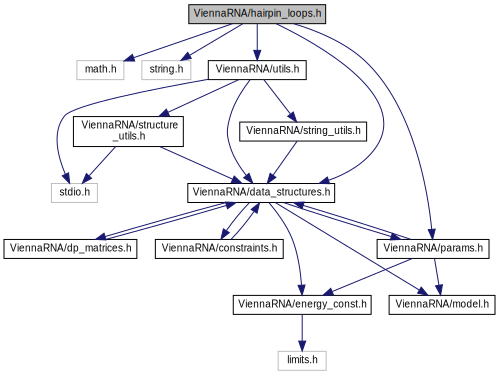
\includegraphics[width=350pt]{hairpin__loops_8h__incl}
\end{center}
\end{figure}
This graph shows which files directly or indirectly include this file\+:
\nopagebreak
\begin{figure}[H]
\begin{center}
\leavevmode
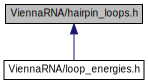
\includegraphics[width=220pt]{hairpin__loops_8h__dep__incl}
\end{center}
\end{figure}
\subsection*{Functions}
\begin{DoxyCompactItemize}
\item 
P\+R\+I\+V\+A\+T\+E int \hyperlink{group__loops_gadf943ee9a45b7f4cee9192c06210dace}{E\+\_\+\+Hairpin} (int size, int type, int si1, int sj1, const char $\ast$string, \hyperlink{group__energy__parameters_ga8a69ca7d787e4fd6079914f5343a1f35}{vrna\+\_\+param\+\_\+t} $\ast$P)
\begin{DoxyCompactList}\small\item\em Compute the Energy of a hairpin-\/loop. \end{DoxyCompactList}\item 
P\+R\+I\+V\+A\+T\+E \hyperlink{group__data__structures_ga31125aeace516926bf7f251f759b6126}{F\+L\+T\+\_\+\+O\+R\+\_\+\+D\+B\+L} \hyperlink{group__loops_ga51fb555974f180b78d76142b2894851c}{exp\+\_\+\+E\+\_\+\+Hairpin} (int u, int type, short si1, short sj1, const char $\ast$string, \hyperlink{group__energy__parameters_ga01d8b92fe734df8d79a6169482c7d8d8}{vrna\+\_\+exp\+\_\+param\+\_\+t} $\ast$P)
\begin{DoxyCompactList}\small\item\em Compute Boltzmann weight $e^{-\Delta G/kT} $ of a hairpin loop. \end{DoxyCompactList}\item 
int \hyperlink{group__eval_gab3eb4651dc26dc2b653a57dd340d7e68}{vrna\+\_\+eval\+\_\+hp\+\_\+loop} (\hyperlink{group__fold__compound_ga1b0cef17fd40466cef5968eaeeff6166}{vrna\+\_\+fold\+\_\+compound\+\_\+t} $\ast$vc, int i, int j)
\begin{DoxyCompactList}\small\item\em Evaluate free energy of a hairpin loop. \end{DoxyCompactList}\item 
\hypertarget{group__eval_gad3b92453a6b501856eec8fae39f3235d}{int \hyperlink{group__eval_gad3b92453a6b501856eec8fae39f3235d}{vrna\+\_\+eval\+\_\+ext\+\_\+hp\+\_\+loop} (\hyperlink{group__fold__compound_ga1b0cef17fd40466cef5968eaeeff6166}{vrna\+\_\+fold\+\_\+compound\+\_\+t} $\ast$vc, int i, int j)}\label{group__eval_gad3b92453a6b501856eec8fae39f3235d}

\begin{DoxyCompactList}\small\item\em Evaluate free energy of an exterior hairpin loop. \end{DoxyCompactList}\item 
int \hyperlink{group__loops_ga999ba163a8148d72fd5f22819a681df7}{vrna\+\_\+\+E\+\_\+hp\+\_\+loop} (\hyperlink{group__fold__compound_ga1b0cef17fd40466cef5968eaeeff6166}{vrna\+\_\+fold\+\_\+compound\+\_\+t} $\ast$vc, int i, int j)
\begin{DoxyCompactList}\small\item\em Evaluate the free energy of a hairpin loop and consider possible hard constraints. \end{DoxyCompactList}\item 
int \hyperlink{group__loops_gac3393ee309372eccae944e3a07f455f9}{vrna\+\_\+\+E\+\_\+ext\+\_\+hp\+\_\+loop} (\hyperlink{group__fold__compound_ga1b0cef17fd40466cef5968eaeeff6166}{vrna\+\_\+fold\+\_\+compound\+\_\+t} $\ast$vc, int i, int j)
\begin{DoxyCompactList}\small\item\em Evaluate the free energy of an exterior hairpin loop and consider possible hard constraints. \end{DoxyCompactList}\item 
\hyperlink{group__data__structures_ga31125aeace516926bf7f251f759b6126}{F\+L\+T\+\_\+\+O\+R\+\_\+\+D\+B\+L} \hyperlink{group__loops_gac9f49b31d3ec1d9040798b05506c71da}{vrna\+\_\+exp\+\_\+\+E\+\_\+hp\+\_\+loop} (\hyperlink{group__fold__compound_ga1b0cef17fd40466cef5968eaeeff6166}{vrna\+\_\+fold\+\_\+compound\+\_\+t} $\ast$vc, int i, int j)
\begin{DoxyCompactList}\small\item\em High-\/\+Level function for hairpin loop energy evaluation (partition function variant) \end{DoxyCompactList}\item 
int \hyperlink{group__loops_ga6c4ba14d24f716d0ca9021771357e903}{vrna\+\_\+\+B\+T\+\_\+hp\+\_\+loop} (\hyperlink{group__fold__compound_ga1b0cef17fd40466cef5968eaeeff6166}{vrna\+\_\+fold\+\_\+compound\+\_\+t} $\ast$vc, int i, int j, int en, \hyperlink{group__data__structures_gaa651bda42e7692f08cb603cd6834b0ee}{vrna\+\_\+bp\+\_\+stack\+\_\+t} $\ast$bp\+\_\+stack, int $\ast$stack\+\_\+count)
\begin{DoxyCompactList}\small\item\em Backtrack a hairpin loop closed by $ (i,j) $. \end{DoxyCompactList}\end{DoxyCompactItemize}


\subsection{Detailed Description}
Energy evaluation of hairpin loops for M\+F\+E and partition function calculations. 


\input{interior__loops_8h}
\hypertarget{inverse_8h}{\section{Vienna\+R\+N\+A/inverse.h File Reference}
\label{inverse_8h}\index{Vienna\+R\+N\+A/inverse.\+h@{Vienna\+R\+N\+A/inverse.\+h}}
}


Inverse folding routines.  


\subsection*{Functions}
\begin{DoxyCompactItemize}
\item 
float \hyperlink{group__inverse__fold_ga7af026de55d4babad879f2c92559cbbc}{inverse\+\_\+fold} (char $\ast$start, const char $\ast$target)
\begin{DoxyCompactList}\small\item\em Find sequences with predefined structure. \end{DoxyCompactList}\item 
float \hyperlink{group__inverse__fold_gaeef52ecbf2a2450ad585a344f9826806}{inverse\+\_\+pf\+\_\+fold} (char $\ast$start, const char $\ast$target)
\begin{DoxyCompactList}\small\item\em Find sequence that maximizes probability of a predefined structure. \end{DoxyCompactList}\end{DoxyCompactItemize}
\subsection*{Variables}
\begin{DoxyCompactItemize}
\item 
\hypertarget{group__inverse__fold_ga8f791e7740a5a28b9f6fafb4e60301d9}{char $\ast$ \hyperlink{group__inverse__fold_ga8f791e7740a5a28b9f6fafb4e60301d9}{symbolset}}\label{group__inverse__fold_ga8f791e7740a5a28b9f6fafb4e60301d9}

\begin{DoxyCompactList}\small\item\em This global variable points to the allowed bases, initially \char`\"{}\+A\+U\+G\+C\char`\"{}. It can be used to design sequences from reduced alphabets. \end{DoxyCompactList}\item 
float \hyperlink{group__inverse__fold_ga7f17d3b169af048d32bb185039a9c09c}{final\+\_\+cost}
\item 
int \hyperlink{group__inverse__fold_ga7ec4ba51f86e1717a1e174264e4a75ce}{give\+\_\+up}
\item 
int \hyperlink{group__inverse__fold_gafcfc65fba01b9cca5946726ed9057a63}{inv\+\_\+verbose}
\end{DoxyCompactItemize}


\subsection{Detailed Description}
Inverse folding routines. 


\input{Lfold_8h}
\input{ligand_8h}
\input{loop__energies_8h}
\hypertarget{LPfold_8h}{}\section{Vienna\+R\+N\+A/\+L\+Pfold.h File Reference}
\label{LPfold_8h}\index{Vienna\+R\+N\+A/\+L\+Pfold.\+h@{Vienna\+R\+N\+A/\+L\+Pfold.\+h}}


Function declarations of partition function variants of the Lfold algorithm.  


Include dependency graph for L\+Pfold.\+h\+:
\nopagebreak
\begin{figure}[H]
\begin{center}
\leavevmode
\includegraphics[width=350pt]{LPfold_8h__incl}
\end{center}
\end{figure}
\subsection*{Functions}
\begin{DoxyCompactItemize}
\item 
void \hyperlink{group__local__pf__fold_ga5a019014d37fe6105131dfc2fc447880}{update\+\_\+pf\+\_\+params\+L\+P} (int length)
\item 
\hyperlink{group__data__structures_gab1d8894b43aa84cbc50b862a73785fbc}{plist} $\ast$ \hyperlink{group__local__pf__fold_ga7dcf599d07258801ea55e7d14a56908d}{pfl\+\_\+fold} (char $\ast$sequence, int win\+Size, int pair\+Size, float cutoffb, double $\ast$$\ast$p\+U, \hyperlink{group__data__structures_gab1d8894b43aa84cbc50b862a73785fbc}{plist} $\ast$$\ast$dpp2, F\+I\+L\+E $\ast$p\+Ufp, F\+I\+L\+E $\ast$spup)
\begin{DoxyCompactList}\small\item\em Compute partition functions for locally stable secondary structures. \end{DoxyCompactList}\item 
\hypertarget{group__local__pf__fold_ga14c2b82fdd5ab7a1951f1c2db4f5cf2c}{}\hyperlink{group__data__structures_gab1d8894b43aa84cbc50b862a73785fbc}{plist} $\ast$ \hyperlink{group__local__pf__fold_ga14c2b82fdd5ab7a1951f1c2db4f5cf2c}{pfl\+\_\+fold\+\_\+par} (char $\ast$sequence, int win\+Size, int pair\+Size, float cutoffb, double $\ast$$\ast$p\+U, \hyperlink{group__data__structures_gab1d8894b43aa84cbc50b862a73785fbc}{plist} $\ast$$\ast$dpp2, F\+I\+L\+E $\ast$p\+Ufp, F\+I\+L\+E $\ast$spup, \hyperlink{group__energy__parameters_ga01d8b92fe734df8d79a6169482c7d8d8}{vrna\+\_\+exp\+\_\+param\+\_\+t} $\ast$parameters)\label{group__local__pf__fold_ga14c2b82fdd5ab7a1951f1c2db4f5cf2c}

\begin{DoxyCompactList}\small\item\em Compute partition functions for locally stable secondary structures. \end{DoxyCompactList}\item 
void \hyperlink{group__local__pf__fold_ga0bcb751860bbf34e3dfee8c2fbdb3ef3}{putoutp\+U\+\_\+prob} (double $\ast$$\ast$p\+U, int length, int ulength, F\+I\+L\+E $\ast$fp, int energies)
\begin{DoxyCompactList}\small\item\em Writes the unpaired probabilities (p\+U) or opening energies into a file. \end{DoxyCompactList}\item 
void \hyperlink{group__local__pf__fold_ga9acb00ee10e96b1ca4ea394cd8bcec75}{putoutp\+U\+\_\+prob\+\_\+bin} (double $\ast$$\ast$p\+U, int length, int ulength, F\+I\+L\+E $\ast$fp, int energies)
\begin{DoxyCompactList}\small\item\em Writes the unpaired probabilities (p\+U) or opening energies into a binary file. \end{DoxyCompactList}\item 
void \hyperlink{LPfold_8h_ae85bf55053e9fb295208be322e0fa07a}{init\+\_\+pf\+\_\+fold\+L\+P} (int length)
\end{DoxyCompactItemize}


\subsection{Detailed Description}
Function declarations of partition function variants of the Lfold algorithm. 



\subsection{Function Documentation}
\hypertarget{LPfold_8h_ae85bf55053e9fb295208be322e0fa07a}{}\index{L\+Pfold.\+h@{L\+Pfold.\+h}!init\+\_\+pf\+\_\+fold\+L\+P@{init\+\_\+pf\+\_\+fold\+L\+P}}
\index{init\+\_\+pf\+\_\+fold\+L\+P@{init\+\_\+pf\+\_\+fold\+L\+P}!L\+Pfold.\+h@{L\+Pfold.\+h}}
\subsubsection[{init\+\_\+pf\+\_\+fold\+L\+P}]{\setlength{\rightskip}{0pt plus 5cm}void init\+\_\+pf\+\_\+fold\+L\+P (
\begin{DoxyParamCaption}
\item[{int}]{length}
\end{DoxyParamCaption}
)}\label{LPfold_8h_ae85bf55053e9fb295208be322e0fa07a}
Dunno if this function was ever used by external programs linking to R\+N\+Alib, but it was declared P\+U\+B\+L\+I\+C before. Anyway, never use this function as it will be removed soon and does nothing at all 
\hypertarget{MEA_8h}{\section{Vienna\+R\+N\+A/\+M\+E\+A.h File Reference}
\label{MEA_8h}\index{Vienna\+R\+N\+A/\+M\+E\+A.\+h@{Vienna\+R\+N\+A/\+M\+E\+A.\+h}}
}


Computes a M\+E\+A (maximum expected accuracy) structure.  


Include dependency graph for M\+E\+A.\+h\+:
\nopagebreak
\begin{figure}[H]
\begin{center}
\leavevmode
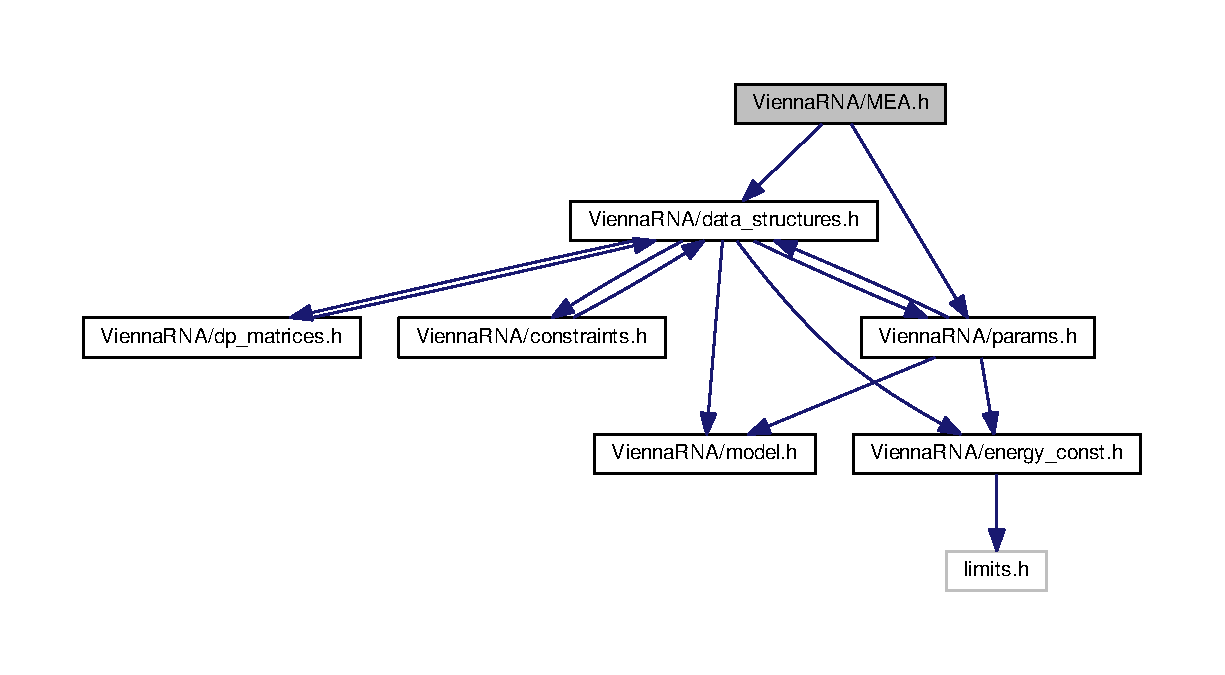
\includegraphics[width=350pt]{MEA_8h__incl}
\end{center}
\end{figure}
\subsection*{Functions}
\begin{DoxyCompactItemize}
\item 
float \hyperlink{MEA_8h_a396ec6144c6a74fcbab4cea6b42d76c3}{M\+E\+A} (\hyperlink{group__data__structures_gab1d8894b43aa84cbc50b862a73785fbc}{plist} $\ast$p, char $\ast$structure, double gamma)
\begin{DoxyCompactList}\small\item\em Computes a M\+E\+A (maximum expected accuracy) structure. \end{DoxyCompactList}\end{DoxyCompactItemize}


\subsection{Detailed Description}
Computes a M\+E\+A (maximum expected accuracy) structure. 



\subsection{Function Documentation}
\hypertarget{MEA_8h_a396ec6144c6a74fcbab4cea6b42d76c3}{\index{M\+E\+A.\+h@{M\+E\+A.\+h}!M\+E\+A@{M\+E\+A}}
\index{M\+E\+A@{M\+E\+A}!M\+E\+A.\+h@{M\+E\+A.\+h}}
\subsubsection[{M\+E\+A}]{\setlength{\rightskip}{0pt plus 5cm}float M\+E\+A (
\begin{DoxyParamCaption}
\item[{{\bf plist} $\ast$}]{p, }
\item[{char $\ast$}]{structure, }
\item[{double}]{gamma}
\end{DoxyParamCaption}
)}}\label{MEA_8h_a396ec6144c6a74fcbab4cea6b42d76c3}


Computes a M\+E\+A (maximum expected accuracy) structure. 

The algorithm maximizes the expected accuracy \[ A(S) = \sum_{(i,j) \in S} 2 \gamma p_{ij} + \sum_{i \notin S} p^u_i \] Higher values of $\gamma$ result in more base pairs of lower probability and thus higher sensitivity. Low values of $\gamma$ result in structures containing only highly likely pairs (high specificity). The code of the M\+E\+A function also demonstrates the use of sparse dynamic programming scheme to reduce the time and memory complexity of folding. 
\input{mfe_8h}
\hypertarget{mm_8h}{}\section{Vienna\+R\+N\+A/mm.h File Reference}
\label{mm_8h}\index{Vienna\+R\+N\+A/mm.\+h@{Vienna\+R\+N\+A/mm.\+h}}


Several Maximum Matching implementations.  




\subsection{Detailed Description}
Several Maximum Matching implementations. 

This file contains the declarations for several maximum matching implementations 
\hypertarget{model_8h}{}\section{Vienna\+R\+N\+A/model.h File Reference}
\label{model_8h}\index{Vienna\+R\+N\+A/model.\+h@{Vienna\+R\+N\+A/model.\+h}}


The model details data structure and its corresponding modifiers.  


This graph shows which files directly or indirectly include this file\+:
\nopagebreak
\begin{figure}[H]
\begin{center}
\leavevmode
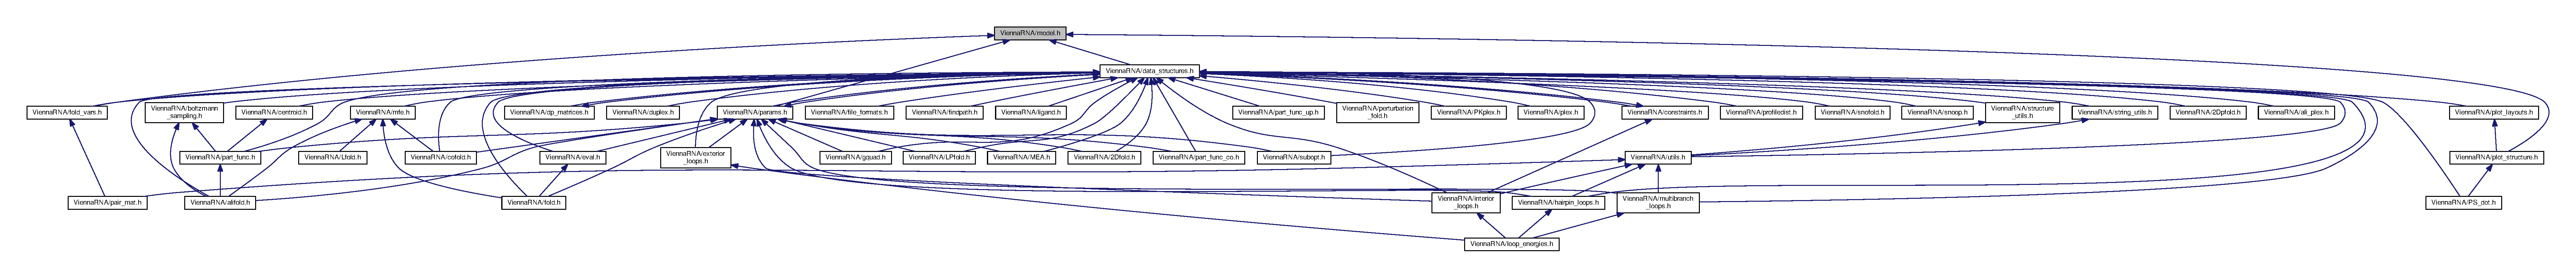
\includegraphics[width=350pt]{model_8h__dep__incl}
\end{center}
\end{figure}
\subsection*{Data Structures}
\begin{DoxyCompactItemize}
\item 
struct \hyperlink{group__model__details_structvrna__md__s}{vrna\+\_\+md\+\_\+s}
\begin{DoxyCompactList}\small\item\em The data structure that contains the complete model details used throughout the calculations.  \hyperlink{group__model__details_structvrna__md__s}{More...}\end{DoxyCompactList}\end{DoxyCompactItemize}
\subsection*{Macros}
\begin{DoxyCompactItemize}
\item 
\#define \hyperlink{group__model__details_gaf47f9850b3b4763479f7a7e7a15648a2}{V\+R\+N\+A\+\_\+\+M\+O\+D\+E\+L\+\_\+\+D\+E\+F\+A\+U\+L\+T\+\_\+\+T\+E\+M\+P\+E\+R\+A\+T\+U\+R\+E}~37.\+0
\begin{DoxyCompactList}\small\item\em   Default temperature for structure prediction and free energy evaluation in $^\circ C$  \end{DoxyCompactList}\item 
\#define \hyperlink{group__model__details_ga5505389cba74a18bbc116d2bb20256fa}{V\+R\+N\+A\+\_\+\+M\+O\+D\+E\+L\+\_\+\+D\+E\+F\+A\+U\+L\+T\+\_\+\+P\+F\+\_\+\+S\+C\+A\+L\+E}~-\/1
\begin{DoxyCompactList}\small\item\em Default scaling factor for partition function computations. \end{DoxyCompactList}\item 
\#define \hyperlink{group__model__details_ga383d3ac8d08c3b6221754b50871c1200}{V\+R\+N\+A\+\_\+\+M\+O\+D\+E\+L\+\_\+\+D\+E\+F\+A\+U\+L\+T\+\_\+\+B\+E\+T\+A\+\_\+\+S\+C\+A\+L\+E}~1.
\begin{DoxyCompactList}\small\item\em Default scaling factor for absolute thermodynamic temperature in Boltzmann factors. \end{DoxyCompactList}\item 
\#define \hyperlink{group__model__details_ga2aa7bc2cae774b83a5c468f824c27a42}{V\+R\+N\+A\+\_\+\+M\+O\+D\+E\+L\+\_\+\+D\+E\+F\+A\+U\+L\+T\+\_\+\+D\+A\+N\+G\+L\+E\+S}~2
\begin{DoxyCompactList}\small\item\em Default dangling end model. \end{DoxyCompactList}\item 
\#define \hyperlink{group__model__details_gabd1ab224e1048defd45c165ed7d1c108}{V\+R\+N\+A\+\_\+\+M\+O\+D\+E\+L\+\_\+\+D\+E\+F\+A\+U\+L\+T\+\_\+\+S\+P\+E\+C\+I\+A\+L\+\_\+\+H\+P}~1
\begin{DoxyCompactList}\small\item\em Default model behavior for lookup of special tri-\/, tetra-\/, and hexa-\/loops. \end{DoxyCompactList}\item 
\#define \hyperlink{group__model__details_gab72462726dd60ed0d43339bbf7ee08ad}{V\+R\+N\+A\+\_\+\+M\+O\+D\+E\+L\+\_\+\+D\+E\+F\+A\+U\+L\+T\+\_\+\+N\+O\+\_\+\+L\+P}~0
\begin{DoxyCompactList}\small\item\em Default model behavior for so-\/called \textquotesingle{}lonely pairs\textquotesingle{}. \end{DoxyCompactList}\item 
\#define \hyperlink{group__model__details_ga34702f7d14d38b877ba8e475281e97e2}{V\+R\+N\+A\+\_\+\+M\+O\+D\+E\+L\+\_\+\+D\+E\+F\+A\+U\+L\+T\+\_\+\+N\+O\+\_\+\+G\+U}~0
\begin{DoxyCompactList}\small\item\em Default model behavior for G-\/\+U base pairs. \end{DoxyCompactList}\item 
\#define \hyperlink{group__model__details_ga5308de46faaca4b9fd16045864901ee7}{V\+R\+N\+A\+\_\+\+M\+O\+D\+E\+L\+\_\+\+D\+E\+F\+A\+U\+L\+T\+\_\+\+N\+O\+\_\+\+G\+U\+\_\+\+C\+L\+O\+S\+U\+R\+E}~0
\begin{DoxyCompactList}\small\item\em Default model behavior for G-\/\+U base pairs closing a loop. \end{DoxyCompactList}\item 
\#define \hyperlink{group__model__details_ga22059033db7bcd875c51fec32425490a}{V\+R\+N\+A\+\_\+\+M\+O\+D\+E\+L\+\_\+\+D\+E\+F\+A\+U\+L\+T\+\_\+\+C\+I\+R\+C}~0
\begin{DoxyCompactList}\small\item\em Default model behavior to treat a molecule as a circular R\+N\+A (D\+N\+A) \end{DoxyCompactList}\item 
\#define \hyperlink{group__model__details_ga793ed812e86f43799b14b2deee917f23}{V\+R\+N\+A\+\_\+\+M\+O\+D\+E\+L\+\_\+\+D\+E\+F\+A\+U\+L\+T\+\_\+\+G\+Q\+U\+A\+D}~0
\begin{DoxyCompactList}\small\item\em Default model behavior regarding the treatment of G-\/\+Quadruplexes. \end{DoxyCompactList}\item 
\#define \hyperlink{group__model__details_ga63f6006a02ba2d89148441f406c309e7}{V\+R\+N\+A\+\_\+\+M\+O\+D\+E\+L\+\_\+\+D\+E\+F\+A\+U\+L\+T\+\_\+\+U\+N\+I\+Q\+\_\+\+M\+L}~0
\begin{DoxyCompactList}\small\item\em Default behavior of the model regarding unique multibranch loop decomposition. \end{DoxyCompactList}\item 
\#define \hyperlink{group__model__details_ga6fcf6b2d0f89256cdbd166486c9b6e1e}{V\+R\+N\+A\+\_\+\+M\+O\+D\+E\+L\+\_\+\+D\+E\+F\+A\+U\+L\+T\+\_\+\+E\+N\+E\+R\+G\+Y\+\_\+\+S\+E\+T}~0
\begin{DoxyCompactList}\small\item\em Default model behavior on which energy set to use. \end{DoxyCompactList}\item 
\#define \hyperlink{group__model__details_ga3fda8006ab84baf817bd8e5ccbc6bb35}{V\+R\+N\+A\+\_\+\+M\+O\+D\+E\+L\+\_\+\+D\+E\+F\+A\+U\+L\+T\+\_\+\+B\+A\+C\+K\+T\+R\+A\+C\+K}~1
\begin{DoxyCompactList}\small\item\em Default model behavior with regards to backtracking of structures. \end{DoxyCompactList}\item 
\#define \hyperlink{group__model__details_gad0e81fcaca53c4a826c68e0796de2afb}{V\+R\+N\+A\+\_\+\+M\+O\+D\+E\+L\+\_\+\+D\+E\+F\+A\+U\+L\+T\+\_\+\+B\+A\+C\+K\+T\+R\+A\+C\+K\+\_\+\+T\+Y\+P\+E}~\textquotesingle{}F\textquotesingle{}
\begin{DoxyCompactList}\small\item\em Default model behavior on what type of backtracking to perform. \end{DoxyCompactList}\item 
\#define \hyperlink{group__model__details_ga1d6cd5051940b126c248147c011bac6c}{V\+R\+N\+A\+\_\+\+M\+O\+D\+E\+L\+\_\+\+D\+E\+F\+A\+U\+L\+T\+\_\+\+C\+O\+M\+P\+U\+T\+E\+\_\+\+B\+P\+P}~1
\begin{DoxyCompactList}\small\item\em Default model behavior with regards to computing base pair probabilities. \end{DoxyCompactList}\item 
\#define \hyperlink{group__model__details_ga7cb6f4ae8fdebff6746a4410814f2977}{V\+R\+N\+A\+\_\+\+M\+O\+D\+E\+L\+\_\+\+D\+E\+F\+A\+U\+L\+T\+\_\+\+M\+A\+X\+\_\+\+B\+P\+\_\+\+S\+P\+A\+N}~-\/1
\begin{DoxyCompactList}\small\item\em Default model behavior for the allowed maximum base pair span. \end{DoxyCompactList}\item 
\#define \hyperlink{group__model__details_ga8de04a9cb57e811e313b0f9f207f6bdb}{V\+R\+N\+A\+\_\+\+M\+O\+D\+E\+L\+\_\+\+D\+E\+F\+A\+U\+L\+T\+\_\+\+W\+I\+N\+D\+O\+W\+\_\+\+S\+I\+Z\+E}~-\/1
\begin{DoxyCompactList}\small\item\em Default model behavior for the sliding window approach. \end{DoxyCompactList}\item 
\#define \hyperlink{group__model__details_ga938f68463e84fe060aa6502f428a517d}{V\+R\+N\+A\+\_\+\+M\+O\+D\+E\+L\+\_\+\+D\+E\+F\+A\+U\+L\+T\+\_\+\+L\+O\+G\+\_\+\+M\+L}~0
\begin{DoxyCompactList}\small\item\em Default model behavior on how to evaluate the energy contribution of multibranch loops. \end{DoxyCompactList}\item 
\#define \hyperlink{group__model__details_ga2a5bbfc1edf33077e39466d2d9807115}{V\+R\+N\+A\+\_\+\+M\+O\+D\+E\+L\+\_\+\+D\+E\+F\+A\+U\+L\+T\+\_\+\+A\+L\+I\+\_\+\+O\+L\+D\+\_\+\+E\+N}~0
\begin{DoxyCompactList}\small\item\em Default model behavior for consensus structure energy evaluation. \end{DoxyCompactList}\item 
\#define \hyperlink{group__model__details_ga64b3ab65a9ca42d4ad1d05e193083147}{V\+R\+N\+A\+\_\+\+M\+O\+D\+E\+L\+\_\+\+D\+E\+F\+A\+U\+L\+T\+\_\+\+A\+L\+I\+\_\+\+R\+I\+B\+O}~0
\begin{DoxyCompactList}\small\item\em Default model behavior for consensus structure covariance contribution assessment. \end{DoxyCompactList}\item 
\#define \hyperlink{group__model__details_gaaaf3d73d6abc18d3889676952bfedb96}{V\+R\+N\+A\+\_\+\+M\+O\+D\+E\+L\+\_\+\+D\+E\+F\+A\+U\+L\+T\+\_\+\+A\+L\+I\+\_\+\+C\+V\+\_\+\+F\+A\+C\+T}~1.
\begin{DoxyCompactList}\small\item\em Default model behavior for weighting the covariance score in consensus structure prediction. \end{DoxyCompactList}\item 
\#define \hyperlink{group__model__details_ga8f774daaafec28160c1ca5d09f2cbdba}{V\+R\+N\+A\+\_\+\+M\+O\+D\+E\+L\+\_\+\+D\+E\+F\+A\+U\+L\+T\+\_\+\+A\+L\+I\+\_\+\+N\+C\+\_\+\+F\+A\+C\+T}~1.
\begin{DoxyCompactList}\small\item\em Default model behavior for weighting the nucleotide conservation? in consensus structure prediction. \end{DoxyCompactList}\item 
\hypertarget{group__model__details_ga05a5ffe718aa431d97419a12fb082379}{}\#define \hyperlink{group__model__details_ga05a5ffe718aa431d97419a12fb082379}{M\+A\+X\+A\+L\+P\+H\+A}~20\label{group__model__details_ga05a5ffe718aa431d97419a12fb082379}

\begin{DoxyCompactList}\small\item\em Maximal length of alphabet. \end{DoxyCompactList}\end{DoxyCompactItemize}
\subsection*{Typedefs}
\begin{DoxyCompactItemize}
\item 
\hypertarget{group__model__details_ga1f8a10e12a0a1915f2a4eff0b28ea17c}{}typedef struct \hyperlink{group__model__details_structvrna__md__s}{vrna\+\_\+md\+\_\+s} \hyperlink{group__model__details_ga1f8a10e12a0a1915f2a4eff0b28ea17c}{vrna\+\_\+md\+\_\+t}\label{group__model__details_ga1f8a10e12a0a1915f2a4eff0b28ea17c}

\begin{DoxyCompactList}\small\item\em Typename for the model details data structure \hyperlink{group__model__details_structvrna__md__s}{vrna\+\_\+md\+\_\+s}. \end{DoxyCompactList}\end{DoxyCompactItemize}
\subsection*{Functions}
\begin{DoxyCompactItemize}
\item 
void \hyperlink{group__model__details_ga8ac6ff84936282436f822644bf841f66}{vrna\+\_\+md\+\_\+set\+\_\+default} (\hyperlink{group__model__details_ga1f8a10e12a0a1915f2a4eff0b28ea17c}{vrna\+\_\+md\+\_\+t} $\ast$md)
\begin{DoxyCompactList}\small\item\em Apply default model details to a provided \hyperlink{group__model__details_ga1f8a10e12a0a1915f2a4eff0b28ea17c}{vrna\+\_\+md\+\_\+t} data structure. \end{DoxyCompactList}\item 
void \hyperlink{group__model__details_ga36ae40b8c3b82362f5798ad5b047b814}{vrna\+\_\+md\+\_\+update} (\hyperlink{group__model__details_ga1f8a10e12a0a1915f2a4eff0b28ea17c}{vrna\+\_\+md\+\_\+t} $\ast$md)
\begin{DoxyCompactList}\small\item\em Update the model details data structure. \end{DoxyCompactList}\item 
char $\ast$ \hyperlink{group__model__details_ga3a7469f0725a849af6ba61a57dfd60ce}{vrna\+\_\+md\+\_\+option\+\_\+string} (\hyperlink{group__model__details_ga1f8a10e12a0a1915f2a4eff0b28ea17c}{vrna\+\_\+md\+\_\+t} $\ast$md)
\begin{DoxyCompactList}\small\item\em Get a corresponding commandline parameter string of the options in a \hyperlink{group__model__details_ga1f8a10e12a0a1915f2a4eff0b28ea17c}{vrna\+\_\+md\+\_\+t}. \end{DoxyCompactList}\item 
void \hyperlink{group__model__details_ga70834424cf804d149937de89f80ceb45}{vrna\+\_\+md\+\_\+defaults\+\_\+reset} (\hyperlink{group__model__details_ga1f8a10e12a0a1915f2a4eff0b28ea17c}{vrna\+\_\+md\+\_\+t} $\ast$md\+\_\+p)
\begin{DoxyCompactList}\small\item\em Reset the global default model details to a specific set of parameters, or their initial values. \end{DoxyCompactList}\item 
void \hyperlink{group__model__details_gaf9e527e9a2f7e6fd6e42bc6e602f5445}{vrna\+\_\+md\+\_\+defaults\+\_\+temperature} (double T)
\begin{DoxyCompactList}\small\item\em Set default temperature for energy evaluation of loops. \end{DoxyCompactList}\item 
double \hyperlink{group__model__details_ga96b24a74437f9ba46c4e06343155bf46}{vrna\+\_\+md\+\_\+defaults\+\_\+temperature\+\_\+get} (void)
\begin{DoxyCompactList}\small\item\em Get default temperature for energy evaluation of loops. \end{DoxyCompactList}\item 
void \hyperlink{group__model__details_gae984567db36c3f9b8731ecc917abf3a2}{vrna\+\_\+md\+\_\+defaults\+\_\+beta\+Scale} (double b)
\begin{DoxyCompactList}\small\item\em Set default scaling factor of thermodynamic temperature in Boltzmann factors. \end{DoxyCompactList}\item 
double \hyperlink{group__model__details_gabb8780f5410c52f970d75b044059bd09}{vrna\+\_\+md\+\_\+defaults\+\_\+beta\+Scale\+\_\+get} (void)
\begin{DoxyCompactList}\small\item\em Get default scaling factor of thermodynamic temperature in Boltzmann factors. \end{DoxyCompactList}\item 
void \hyperlink{group__model__details_gac76a5374def8e5e4e644ff6e4cc72dee}{vrna\+\_\+md\+\_\+defaults\+\_\+dangles} (int d)
\begin{DoxyCompactList}\small\item\em Set default dangle model for structure prediction. \end{DoxyCompactList}\item 
int \hyperlink{group__model__details_ga67ca06f95ae133778c79a4493c9817b8}{vrna\+\_\+md\+\_\+defaults\+\_\+dangles\+\_\+get} (void)
\begin{DoxyCompactList}\small\item\em Get default dangle model for structure prediction. \end{DoxyCompactList}\item 
void \hyperlink{group__model__details_gafff6449a02744add0308e653230c15fc}{vrna\+\_\+md\+\_\+defaults\+\_\+special\+\_\+hp} (int flag)
\begin{DoxyCompactList}\small\item\em Set default behavior for lookup of tabulated free energies for special hairpin loops, such as Tri-\/, Tetra-\/, or Hexa-\/loops. \end{DoxyCompactList}\item 
int \hyperlink{group__model__details_ga1d68a6efdaa1253cc63fd9cd06452559}{vrna\+\_\+md\+\_\+defaults\+\_\+special\+\_\+hp\+\_\+get} (void)
\begin{DoxyCompactList}\small\item\em Get default behavior for lookup of tabulated free energies for special hairpin loops, such as Tri-\/, Tetra-\/, or Hexa-\/loops. \end{DoxyCompactList}\item 
void \hyperlink{group__model__details_ga2f88ffc393ac9d7987849c965fd29ea8}{vrna\+\_\+md\+\_\+defaults\+\_\+no\+L\+P} (int flag)
\begin{DoxyCompactList}\small\item\em Set default behavior for prediction of canonical secondary structures. \end{DoxyCompactList}\item 
int \hyperlink{group__model__details_ga934344888fbacaed538bbbfe910f2aa6}{vrna\+\_\+md\+\_\+defaults\+\_\+no\+L\+P\+\_\+get} (void)
\begin{DoxyCompactList}\small\item\em Get default behavior for prediction of canonical secondary structures. \end{DoxyCompactList}\item 
void \hyperlink{group__model__details_ga98218f85c7a957a1d1ddf4627fdf5a39}{vrna\+\_\+md\+\_\+defaults\+\_\+no\+G\+U} (int flag)
\begin{DoxyCompactList}\small\item\em Set default behavior for treatment of G-\/\+U wobble pairs. \end{DoxyCompactList}\item 
int \hyperlink{group__model__details_ga5faa7d4e536d7fe36ec25428c0cf2563}{vrna\+\_\+md\+\_\+defaults\+\_\+no\+G\+U\+\_\+get} (void)
\begin{DoxyCompactList}\small\item\em Get default behavior for treatment of G-\/\+U wobble pairs. \end{DoxyCompactList}\item 
void \hyperlink{group__model__details_gade5b9951d71ca2fb357a4e6c0c18ccd1}{vrna\+\_\+md\+\_\+defaults\+\_\+no\+G\+Uclosure} (int flag)
\begin{DoxyCompactList}\small\item\em Set default behavior for G-\/\+U pairs as closing pair for loops. \end{DoxyCompactList}\item 
int \hyperlink{group__model__details_ga4f7fdad083243a5348d63320ddaa70f3}{vrna\+\_\+md\+\_\+defaults\+\_\+no\+G\+Uclosure\+\_\+get} (void)
\begin{DoxyCompactList}\small\item\em Get default behavior for G-\/\+U pairs as closing pair for loops. \end{DoxyCompactList}\item 
void \hyperlink{group__model__details_ga3de50a73455d88c3957386933b8e1f90}{vrna\+\_\+md\+\_\+defaults\+\_\+log\+M\+L} (int flag)
\begin{DoxyCompactList}\small\item\em Set default behavior recomputing free energies of multibranch loops using a logarithmic model. \end{DoxyCompactList}\item 
int \hyperlink{group__model__details_ga93f04e070d529c5d0bb87c9681f6ad29}{vrna\+\_\+md\+\_\+defaults\+\_\+log\+M\+L\+\_\+get} (void)
\begin{DoxyCompactList}\small\item\em Get default behavior recomputing free energies of multibranch loops using a logarithmic model. \end{DoxyCompactList}\item 
void \hyperlink{group__model__details_ga4e1deb3e91a8a99e5c6dd905a5eb0186}{vrna\+\_\+md\+\_\+defaults\+\_\+circ} (int flag)
\begin{DoxyCompactList}\small\item\em Set default behavior whether input sequences are circularized. \end{DoxyCompactList}\item 
int \hyperlink{group__model__details_gad3a7e58de344ad93a08925f58f94f6fb}{vrna\+\_\+md\+\_\+defaults\+\_\+circ\+\_\+get} (void)
\begin{DoxyCompactList}\small\item\em Get default behavior whether input sequences are circularized. \end{DoxyCompactList}\item 
void \hyperlink{group__model__details_ga0685ca2aeb39af76f2421fc308163dce}{vrna\+\_\+md\+\_\+defaults\+\_\+gquad} (int flag)
\begin{DoxyCompactList}\small\item\em Set default behavior for treatment of G-\/\+Quadruplexes. \end{DoxyCompactList}\item 
int \hyperlink{group__model__details_gae645b8612f879eb38b45244fa9eddb9e}{vrna\+\_\+md\+\_\+defaults\+\_\+gquad\+\_\+get} (void)
\begin{DoxyCompactList}\small\item\em Get default behavior for treatment of G-\/\+Quadruplexes. \end{DoxyCompactList}\item 
void \hyperlink{group__model__details_ga59b944f61c5d2babec2d4c48c820de67}{vrna\+\_\+md\+\_\+defaults\+\_\+uniq\+\_\+\+M\+L} (int flag)
\begin{DoxyCompactList}\small\item\em Set default behavior for creating additional matrix for unique multibranch loop prediction. \end{DoxyCompactList}\item 
int \hyperlink{group__model__details_gab48e70fd024bf838404bcbcca0c874a0}{vrna\+\_\+md\+\_\+defaults\+\_\+uniq\+\_\+\+M\+L\+\_\+get} (void)
\begin{DoxyCompactList}\small\item\em Get default behavior for creating additional matrix for unique multibranch loop prediction. \end{DoxyCompactList}\item 
void \hyperlink{group__model__details_ga8dd29c55787a4576277e1907e92d810c}{vrna\+\_\+md\+\_\+defaults\+\_\+energy\+\_\+set} (int e)
\begin{DoxyCompactList}\small\item\em Set default energy set. \end{DoxyCompactList}\item 
int \hyperlink{group__model__details_ga017ed6afb1cba2b7f242412cab618b53}{vrna\+\_\+md\+\_\+defaults\+\_\+energy\+\_\+set\+\_\+get} (void)
\begin{DoxyCompactList}\small\item\em Get default energy set. \end{DoxyCompactList}\item 
void \hyperlink{group__model__details_ga978c468b2fe96a70d5191e3dd17d5599}{vrna\+\_\+md\+\_\+defaults\+\_\+backtrack} (int flag)
\begin{DoxyCompactList}\small\item\em Set default behavior for whether to backtrack secondary structures. \end{DoxyCompactList}\item 
int \hyperlink{group__model__details_ga90da1156e6883ddd68527c2830706648}{vrna\+\_\+md\+\_\+defaults\+\_\+backtrack\+\_\+get} (void)
\begin{DoxyCompactList}\small\item\em Get default behavior for whether to backtrack secondary structures. \end{DoxyCompactList}\item 
void \hyperlink{group__model__details_ga68305274de96b56b7799575e222560d8}{vrna\+\_\+md\+\_\+defaults\+\_\+backtrack\+\_\+type} (char t)
\begin{DoxyCompactList}\small\item\em Set default backtrack type, i.\+e. which D\+P matrix is used. \end{DoxyCompactList}\item 
char \hyperlink{group__model__details_ga1425b4ebd0e034dead66d79becd64143}{vrna\+\_\+md\+\_\+defaults\+\_\+backtrack\+\_\+type\+\_\+get} (void)
\begin{DoxyCompactList}\small\item\em Get default backtrack type, i.\+e. which D\+P matrix is used. \end{DoxyCompactList}\item 
void \hyperlink{group__model__details_gaf1b5db10f1f476767f9a95f8a78e3132}{vrna\+\_\+md\+\_\+defaults\+\_\+compute\+\_\+bpp} (int flag)
\begin{DoxyCompactList}\small\item\em Set the default behavior for whether to compute base pair probabilities after partition function computation. \end{DoxyCompactList}\item 
int \hyperlink{group__model__details_gaa3a537e61fbe0518673bf9f73fd820f3}{vrna\+\_\+md\+\_\+defaults\+\_\+compute\+\_\+bpp\+\_\+get} (void)
\begin{DoxyCompactList}\small\item\em Get the default behavior for whether to compute base pair probabilities after partition function computation. \end{DoxyCompactList}\item 
void \hyperlink{group__model__details_ga4c4bc962f09b4480cb8499f1cf8ae4ec}{vrna\+\_\+md\+\_\+defaults\+\_\+max\+\_\+bp\+\_\+span} (int span)
\begin{DoxyCompactList}\small\item\em Set default maximal base pair span. \end{DoxyCompactList}\item 
int \hyperlink{group__model__details_gaa60f989e062fecd4d4bac89c1883da85}{vrna\+\_\+md\+\_\+defaults\+\_\+max\+\_\+bp\+\_\+span\+\_\+get} (void)
\begin{DoxyCompactList}\small\item\em Get default maximal base pair span. \end{DoxyCompactList}\item 
void \hyperlink{group__model__details_gac152f1e78c1058a10261022c8dfda0f7}{vrna\+\_\+md\+\_\+defaults\+\_\+min\+\_\+loop\+\_\+size} (int size)
\begin{DoxyCompactList}\small\item\em Set default minimal loop size. \end{DoxyCompactList}\item 
int \hyperlink{group__model__details_ga5cc691174a75c652807dc361b617632a}{vrna\+\_\+md\+\_\+defaults\+\_\+min\+\_\+loop\+\_\+size\+\_\+get} (void)
\begin{DoxyCompactList}\small\item\em Get default minimal loop size. \end{DoxyCompactList}\item 
void \hyperlink{group__model__details_ga7b802ce0e8c3181bf5cb580de6d5b26a}{vrna\+\_\+md\+\_\+defaults\+\_\+window\+\_\+size} (int size)
\begin{DoxyCompactList}\small\item\em Set default window size for sliding window structure prediction approaches. \end{DoxyCompactList}\item 
int \hyperlink{group__model__details_ga670146a9aa3ba77f4d422d60b7c30ac9}{vrna\+\_\+md\+\_\+defaults\+\_\+window\+\_\+size\+\_\+get} (void)
\begin{DoxyCompactList}\small\item\em Get default window size for sliding window structure prediction approaches. \end{DoxyCompactList}\item 
void \hyperlink{group__model__details_ga41521d5b9fb7e0f31e7ea73f5792afab}{vrna\+\_\+md\+\_\+defaults\+\_\+old\+Ali\+En} (int flag)
\begin{DoxyCompactList}\small\item\em Set default behavior for whether to use old energy model for comparative structure prediction. \end{DoxyCompactList}\item 
int \hyperlink{group__model__details_ga2374492b5019df88022fe4c05f0f3630}{vrna\+\_\+md\+\_\+defaults\+\_\+old\+Ali\+En\+\_\+get} (void)
\begin{DoxyCompactList}\small\item\em Get default behavior for whether to use old energy model for comparative structure prediction. \end{DoxyCompactList}\item 
void \hyperlink{group__model__details_ga937c45e1d06fd6168730a9b08d130be3}{vrna\+\_\+md\+\_\+defaults\+\_\+ribo} (int flag)
\begin{DoxyCompactList}\small\item\em Set default behavior for whether to use Ribosum Scoring in comparative structure prediction. \end{DoxyCompactList}\item 
int \hyperlink{group__model__details_ga169027f0c0561ea7d87b655e4b336bfc}{vrna\+\_\+md\+\_\+defaults\+\_\+ribo\+\_\+get} (void)
\begin{DoxyCompactList}\small\item\em Get default behavior for whether to use Ribosum Scoring in comparative structure prediction. \end{DoxyCompactList}\item 
void \hyperlink{group__model__details_gad3a3f40baafd91a6ce80a91a68e20053}{vrna\+\_\+md\+\_\+defaults\+\_\+cv\+\_\+fact} (double factor)
\begin{DoxyCompactList}\small\item\em Set the default covariance scaling factor used in comparative structure prediction. \end{DoxyCompactList}\item 
double \hyperlink{group__model__details_gae59c68393807217b0a2497adb64d3ee3}{vrna\+\_\+md\+\_\+defaults\+\_\+cv\+\_\+fact\+\_\+get} (void)
\begin{DoxyCompactList}\small\item\em Get the default covariance scaling factor used in comparative structure prediction. \end{DoxyCompactList}\item 
void \hyperlink{group__model__details_gac35e596c850dce3ad55c49119fd7d471}{vrna\+\_\+md\+\_\+defaults\+\_\+nc\+\_\+fact} (double factor)
\item 
double \hyperlink{group__model__details_ga7ac759eaa7159bf5f022745f5da59508}{vrna\+\_\+md\+\_\+defaults\+\_\+nc\+\_\+fact\+\_\+get} (void)
\item 
void \hyperlink{group__model__details_ga3f73d3029d3d0025d4cc311510cd95a3}{vrna\+\_\+md\+\_\+defaults\+\_\+sfact} (double factor)
\begin{DoxyCompactList}\small\item\em Set the default scaling factor used to avoid under-\//overflows in partition function computation. \end{DoxyCompactList}\item 
double \hyperlink{group__model__details_gab2df6aab954b63fd3592d18e90285dae}{vrna\+\_\+md\+\_\+defaults\+\_\+sfact\+\_\+get} (void)
\begin{DoxyCompactList}\small\item\em Get the default scaling factor used to avoid under-\//overflows in partition function computation. \end{DoxyCompactList}\item 
void \hyperlink{group__model__details_gabad896c3650d420f3f3ddefc69e2bceb}{set\+\_\+model\+\_\+details} (\hyperlink{group__model__details_ga1f8a10e12a0a1915f2a4eff0b28ea17c}{vrna\+\_\+md\+\_\+t} $\ast$md)
\begin{DoxyCompactList}\small\item\em Set default model details. \end{DoxyCompactList}\end{DoxyCompactItemize}
\subsection*{Variables}
\begin{DoxyCompactItemize}
\item 
double \hyperlink{group__model__details_gab4b11c8d9c758430960896bc3fe82ead}{temperature}
\begin{DoxyCompactList}\small\item\em Rescale energy parameters to a temperature in deg\+C. \end{DoxyCompactList}\item 
double \hyperlink{group__model__details_gad3b22044065acc6dee0af68931b52cfd}{pf\+\_\+scale}
\begin{DoxyCompactList}\small\item\em A scaling factor used by \hyperlink{group__pf__fold_gadc3db3d98742427e7001a7fd36ef28c2}{pf\+\_\+fold()} to avoid overflows. \end{DoxyCompactList}\item 
int \hyperlink{group__model__details_ga72b511ed1201f7e23ec437e468790d74}{dangles}
\begin{DoxyCompactList}\small\item\em Switch the energy model for dangling end contributions (0, 1, 2, 3) \end{DoxyCompactList}\item 
int \hyperlink{group__model__details_ga4f6265bdf0ead7ff4628a360adbfd77e}{tetra\+\_\+loop}
\begin{DoxyCompactList}\small\item\em Include special stabilizing energies for some tri-\/, tetra-\/ and hexa-\/loops;. \end{DoxyCompactList}\item 
int \hyperlink{group__model__details_ga097eccaabd6ae8b4fef83cccff85bb5d}{no\+Lonely\+Pairs}
\begin{DoxyCompactList}\small\item\em Global switch to avoid/allow helices of length 1. \end{DoxyCompactList}\item 
\hypertarget{group__model__details_gabf380d09e4f1ab94fc6af57cf0ad5d32}{}int \hyperlink{group__model__details_gabf380d09e4f1ab94fc6af57cf0ad5d32}{no\+G\+U}\label{group__model__details_gabf380d09e4f1ab94fc6af57cf0ad5d32}

\begin{DoxyCompactList}\small\item\em Global switch to forbid/allow G\+U base pairs at all. \end{DoxyCompactList}\item 
\hypertarget{group__model__details_gaa8d1c7b92489179e1eafa562b7bdd259}{}int \hyperlink{group__model__details_gaa8d1c7b92489179e1eafa562b7bdd259}{no\+\_\+closing\+G\+U}\label{group__model__details_gaa8d1c7b92489179e1eafa562b7bdd259}

\begin{DoxyCompactList}\small\item\em G\+U allowed only inside stacks if set to 1. \end{DoxyCompactList}\item 
\hypertarget{group__model__details_gaf9202a1a09f5828dc731e2d9a10fa111}{}int \hyperlink{group__model__details_gaf9202a1a09f5828dc731e2d9a10fa111}{circ}\label{group__model__details_gaf9202a1a09f5828dc731e2d9a10fa111}

\begin{DoxyCompactList}\small\item\em backward compatibility variable.. this does not effect anything \end{DoxyCompactList}\item 
\hypertarget{group__model__details_ga25f2bdcdf56e813d288845484a13d704}{}int \hyperlink{group__model__details_ga25f2bdcdf56e813d288845484a13d704}{gquad}\label{group__model__details_ga25f2bdcdf56e813d288845484a13d704}

\begin{DoxyCompactList}\small\item\em Allow G-\/quadruplex formation. \end{DoxyCompactList}\item 
int \hyperlink{group__model__details_ga22ae821b8918930e20ffa3fa84802b4b}{canonical\+B\+Ponly}
\item 
\hypertarget{group__model__details_ga6c5655c8b272e3e6cab74dd0f540294f}{}int \hyperlink{group__model__details_ga6c5655c8b272e3e6cab74dd0f540294f}{uniq\+\_\+\+M\+L}\label{group__model__details_ga6c5655c8b272e3e6cab74dd0f540294f}

\begin{DoxyCompactList}\small\item\em do M\+L decomposition uniquely (for subopt) \end{DoxyCompactList}\item 
int \hyperlink{group__model__details_gafb1ef1166da85092ae8a325e02dcae71}{energy\+\_\+set}
\begin{DoxyCompactList}\small\item\em 0 = B\+P; 1=any mit G\+C; 2=any mit A\+U-\/parameter \end{DoxyCompactList}\item 
int \hyperlink{group__model__details_gad512b5dd4dbec60faccfe137bb474489}{do\+\_\+backtrack}
\begin{DoxyCompactList}\small\item\em do backtracking, i.\+e. compute secondary structures or base pair probabilities \end{DoxyCompactList}\item 
char \hyperlink{group__model__details_ga83bdb43472a259c71e69fa9f70f420c3}{backtrack\+\_\+type}
\begin{DoxyCompactList}\small\item\em A backtrack array marker for \hyperlink{group__inverse__fold_ga7af026de55d4babad879f2c92559cbbc}{inverse\+\_\+fold()} \end{DoxyCompactList}\item 
char $\ast$ \hyperlink{group__model__details_ga2695d91cc535d09c2eae5c3884e2ec64}{nonstandards}
\begin{DoxyCompactList}\small\item\em contains allowed non standard base pairs \end{DoxyCompactList}\item 
int \hyperlink{group__model__details_ga18df869af0d70101106458fc3f027806}{max\+\_\+bp\+\_\+span}
\begin{DoxyCompactList}\small\item\em Maximum allowed base pair span. \end{DoxyCompactList}\item 
\hypertarget{group__model__details_gac408868ba00671cbc7d1d535105af045}{}int \hyperlink{group__model__details_gac408868ba00671cbc7d1d535105af045}{old\+Ali\+En}\label{group__model__details_gac408868ba00671cbc7d1d535105af045}

\begin{DoxyCompactList}\small\item\em use old alifold energies (with gaps) \end{DoxyCompactList}\item 
\hypertarget{group__model__details_ga0656afca1d2853f9ee6591172f5638de}{}int \hyperlink{group__model__details_ga0656afca1d2853f9ee6591172f5638de}{ribo}\label{group__model__details_ga0656afca1d2853f9ee6591172f5638de}

\begin{DoxyCompactList}\small\item\em use ribosum matrices \end{DoxyCompactList}\item 
\hypertarget{group__model__details_ga80c3c5fd35e7479704cc91d2d0367743}{}int \hyperlink{group__model__details_ga80c3c5fd35e7479704cc91d2d0367743}{log\+M\+L}\label{group__model__details_ga80c3c5fd35e7479704cc91d2d0367743}

\begin{DoxyCompactList}\small\item\em if nonzero use logarithmic M\+L energy in energy\+\_\+of\+\_\+struct \end{DoxyCompactList}\end{DoxyCompactItemize}


\subsection{Detailed Description}
The model details data structure and its corresponding modifiers. 


\input{multibranch__loops_8h}
\hypertarget{naview_8h}{}\section{Vienna\+R\+N\+A/naview.h File Reference}
\label{naview_8h}\index{Vienna\+R\+N\+A/naview.\+h@{Vienna\+R\+N\+A/naview.\+h}}
This graph shows which files directly or indirectly include this file\+:
\nopagebreak
\begin{figure}[H]
\begin{center}
\leavevmode
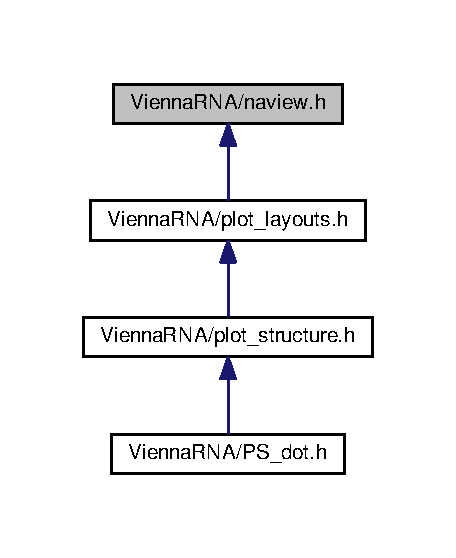
\includegraphics[width=219pt]{naview_8h__dep__incl}
\end{center}
\end{figure}

\hypertarget{params_8h}{}\section{Vienna\+R\+N\+A/params.h File Reference}
\label{params_8h}\index{Vienna\+R\+N\+A/params.\+h@{Vienna\+R\+N\+A/params.\+h}}
Include dependency graph for params.\+h\+:
\nopagebreak
\begin{figure}[H]
\begin{center}
\leavevmode
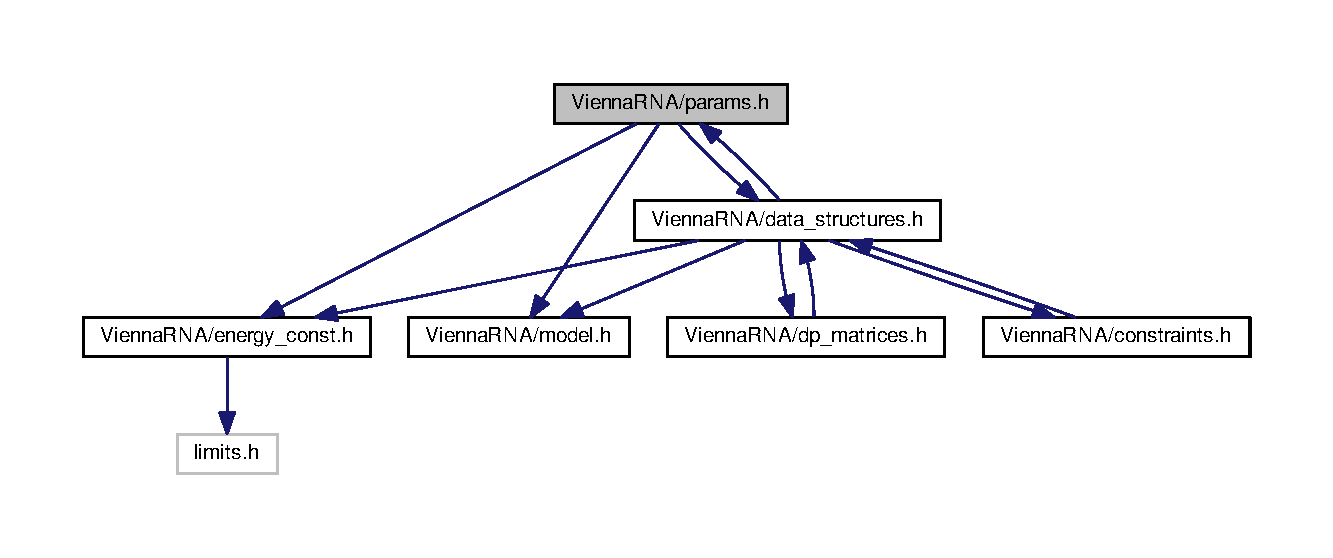
\includegraphics[width=350pt]{params_8h__incl}
\end{center}
\end{figure}
This graph shows which files directly or indirectly include this file\+:
\nopagebreak
\begin{figure}[H]
\begin{center}
\leavevmode
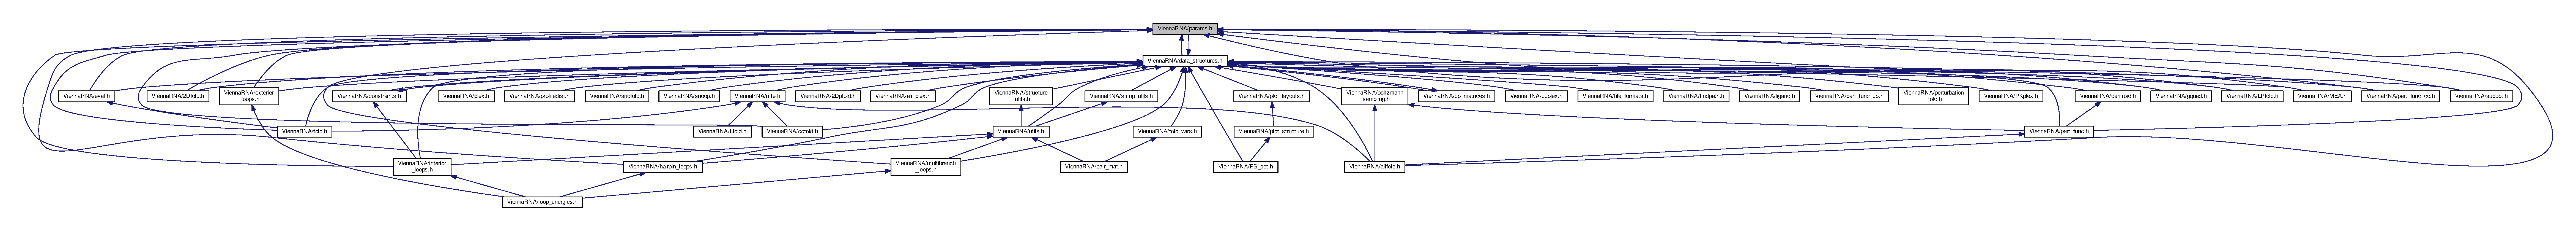
\includegraphics[width=350pt]{params_8h__dep__incl}
\end{center}
\end{figure}
\subsection*{Data Structures}
\begin{DoxyCompactItemize}
\item 
struct \hyperlink{group__energy__parameters_structvrna__param__s}{vrna\+\_\+param\+\_\+s}
\begin{DoxyCompactList}\small\item\em The datastructure that contains temperature scaled energy parameters.  \hyperlink{group__energy__parameters_structvrna__param__s}{More...}\end{DoxyCompactList}\item 
struct \hyperlink{group__energy__parameters_structvrna__exp__param__s}{vrna\+\_\+exp\+\_\+param\+\_\+s}
\begin{DoxyCompactList}\small\item\em The datastructure that contains temperature scaled Boltzmann weights of the energy parameters.  \hyperlink{group__energy__parameters_structvrna__exp__param__s}{More...}\end{DoxyCompactList}\end{DoxyCompactItemize}
\subsection*{Typedefs}
\begin{DoxyCompactItemize}
\item 
\hypertarget{group__energy__parameters_ga8a69ca7d787e4fd6079914f5343a1f35}{}typedef struct \hyperlink{group__energy__parameters_structvrna__param__s}{vrna\+\_\+param\+\_\+s} \hyperlink{group__energy__parameters_ga8a69ca7d787e4fd6079914f5343a1f35}{vrna\+\_\+param\+\_\+t}\label{group__energy__parameters_ga8a69ca7d787e4fd6079914f5343a1f35}

\begin{DoxyCompactList}\small\item\em Typename for the free energy parameter data structure \hyperlink{group__energy__parameters_gad0e3e7e74bdc50d1709d40c92993185e}{vrna\+\_\+params}. \end{DoxyCompactList}\item 
\hypertarget{group__energy__parameters_ga01d8b92fe734df8d79a6169482c7d8d8}{}typedef struct \hyperlink{group__energy__parameters_structvrna__exp__param__s}{vrna\+\_\+exp\+\_\+param\+\_\+s} \hyperlink{group__energy__parameters_ga01d8b92fe734df8d79a6169482c7d8d8}{vrna\+\_\+exp\+\_\+param\+\_\+t}\label{group__energy__parameters_ga01d8b92fe734df8d79a6169482c7d8d8}

\begin{DoxyCompactList}\small\item\em Typename for the Boltzmann factor data structure \hyperlink{group__energy__parameters_gab1f3016f96aa96bff020cdd904605afa}{vrna\+\_\+exp\+\_\+params}. \end{DoxyCompactList}\item 
typedef struct \hyperlink{group__energy__parameters_structvrna__param__s}{vrna\+\_\+param\+\_\+s} \hyperlink{group__energy__parameters_ga857dde86357d306cc902f0d8b2797659}{param\+T}
\begin{DoxyCompactList}\small\item\em Old typename of \hyperlink{group__energy__parameters_structvrna__param__s}{vrna\+\_\+param\+\_\+s}. \end{DoxyCompactList}\item 
typedef struct \hyperlink{group__energy__parameters_structvrna__exp__param__s}{vrna\+\_\+exp\+\_\+param\+\_\+s} \hyperlink{group__energy__parameters_ga8bffe1828e2cbec101769f5cc0b1535b}{pf\+\_\+param\+T}
\begin{DoxyCompactList}\small\item\em Old typename of \#vrna\+\_\+ex\+\_\+param\+\_\+s. \end{DoxyCompactList}\end{DoxyCompactItemize}
\subsection*{Functions}
\begin{DoxyCompactItemize}
\item 
\hyperlink{group__energy__parameters_ga8a69ca7d787e4fd6079914f5343a1f35}{vrna\+\_\+param\+\_\+t} $\ast$ \hyperlink{group__energy__parameters_gad0e3e7e74bdc50d1709d40c92993185e}{vrna\+\_\+params} (\hyperlink{group__model__details_ga1f8a10e12a0a1915f2a4eff0b28ea17c}{vrna\+\_\+md\+\_\+t} $\ast$md)
\begin{DoxyCompactList}\small\item\em Get a data structure containing prescaled free energy parameters. \end{DoxyCompactList}\item 
\hyperlink{group__energy__parameters_ga8a69ca7d787e4fd6079914f5343a1f35}{vrna\+\_\+param\+\_\+t} $\ast$ \hyperlink{group__energy__parameters_ga4bffa39f26e7746148444dd8a8426eca}{vrna\+\_\+params\+\_\+copy} (\hyperlink{group__energy__parameters_ga8a69ca7d787e4fd6079914f5343a1f35}{vrna\+\_\+param\+\_\+t} $\ast$par)
\begin{DoxyCompactList}\small\item\em Get a copy of the provided free energy parameters. \end{DoxyCompactList}\item 
\hyperlink{group__energy__parameters_ga01d8b92fe734df8d79a6169482c7d8d8}{vrna\+\_\+exp\+\_\+param\+\_\+t} $\ast$ \hyperlink{group__energy__parameters_gab1f3016f96aa96bff020cdd904605afa}{vrna\+\_\+exp\+\_\+params} (\hyperlink{group__model__details_ga1f8a10e12a0a1915f2a4eff0b28ea17c}{vrna\+\_\+md\+\_\+t} $\ast$md)
\begin{DoxyCompactList}\small\item\em Get a data structure containing prescaled free energy parameters already transformed to Boltzmann factors. \end{DoxyCompactList}\item 
\hyperlink{group__energy__parameters_ga01d8b92fe734df8d79a6169482c7d8d8}{vrna\+\_\+exp\+\_\+param\+\_\+t} $\ast$ \hyperlink{group__energy__parameters_gaf78c09e685e6eef4100b1a41d4042550}{vrna\+\_\+exp\+\_\+params\+\_\+comparative} (unsigned int n\+\_\+seq, \hyperlink{group__model__details_ga1f8a10e12a0a1915f2a4eff0b28ea17c}{vrna\+\_\+md\+\_\+t} $\ast$md)
\begin{DoxyCompactList}\small\item\em Get a data structure containing prescaled free energy parameters already transformed to Boltzmann factors (alifold version) \end{DoxyCompactList}\item 
\hyperlink{group__energy__parameters_ga01d8b92fe734df8d79a6169482c7d8d8}{vrna\+\_\+exp\+\_\+param\+\_\+t} $\ast$ \hyperlink{group__energy__parameters_ga70bc46be7cfa5434a71efe241c4f0609}{vrna\+\_\+exp\+\_\+params\+\_\+copy} (\hyperlink{group__energy__parameters_ga01d8b92fe734df8d79a6169482c7d8d8}{vrna\+\_\+exp\+\_\+param\+\_\+t} $\ast$par)
\begin{DoxyCompactList}\small\item\em Get a copy of the provided free energy parameters (provided as Boltzmann factors) \end{DoxyCompactList}\item 
void \hyperlink{group__energy__parameters_ga5d1909208f7ea3baa98b75afaa1f62ca}{vrna\+\_\+params\+\_\+subst} (\hyperlink{group__fold__compound_ga1b0cef17fd40466cef5968eaeeff6166}{vrna\+\_\+fold\+\_\+compound\+\_\+t} $\ast$vc, \hyperlink{group__energy__parameters_ga8a69ca7d787e4fd6079914f5343a1f35}{vrna\+\_\+param\+\_\+t} $\ast$par)
\begin{DoxyCompactList}\small\item\em Update/\+Reset energy parameters data structure within a \hyperlink{group__fold__compound_ga1b0cef17fd40466cef5968eaeeff6166}{vrna\+\_\+fold\+\_\+compound\+\_\+t}. \end{DoxyCompactList}\item 
void \hyperlink{group__energy__parameters_ga8e7ac4fab3b0cc03afbc134eaafb3525}{vrna\+\_\+exp\+\_\+params\+\_\+subst} (\hyperlink{group__fold__compound_ga1b0cef17fd40466cef5968eaeeff6166}{vrna\+\_\+fold\+\_\+compound\+\_\+t} $\ast$vc, \hyperlink{group__energy__parameters_ga01d8b92fe734df8d79a6169482c7d8d8}{vrna\+\_\+exp\+\_\+param\+\_\+t} $\ast$params)
\begin{DoxyCompactList}\small\item\em Update the energy parameters for subsequent partition function computations. \end{DoxyCompactList}\item 
void \hyperlink{group__energy__parameters_gad607bc3a5b5da16400e2ca4ea5560233}{vrna\+\_\+exp\+\_\+params\+\_\+rescale} (\hyperlink{group__fold__compound_ga1b0cef17fd40466cef5968eaeeff6166}{vrna\+\_\+fold\+\_\+compound\+\_\+t} $\ast$vc, double $\ast$mfe)
\begin{DoxyCompactList}\small\item\em Rescale Boltzmann factors for partition function computations. \end{DoxyCompactList}\item 
void \hyperlink{group__energy__parameters_gac40dc82e48a72a97cfc58b9da08a7792}{vrna\+\_\+params\+\_\+reset} (\hyperlink{group__fold__compound_ga1b0cef17fd40466cef5968eaeeff6166}{vrna\+\_\+fold\+\_\+compound\+\_\+t} $\ast$vc, \hyperlink{group__model__details_ga1f8a10e12a0a1915f2a4eff0b28ea17c}{vrna\+\_\+md\+\_\+t} $\ast$md\+\_\+p)
\begin{DoxyCompactList}\small\item\em Reset free energy parameters within a \hyperlink{group__fold__compound_ga1b0cef17fd40466cef5968eaeeff6166}{vrna\+\_\+fold\+\_\+compound\+\_\+t} according to provided, or default model details. \end{DoxyCompactList}\item 
void \hyperlink{group__energy__parameters_gae3c6f8897fb1f824e7fa55ab179aa3e8}{vrna\+\_\+exp\+\_\+params\+\_\+reset} (\hyperlink{group__fold__compound_ga1b0cef17fd40466cef5968eaeeff6166}{vrna\+\_\+fold\+\_\+compound\+\_\+t} $\ast$vc, \hyperlink{group__model__details_ga1f8a10e12a0a1915f2a4eff0b28ea17c}{vrna\+\_\+md\+\_\+t} $\ast$md\+\_\+p)
\begin{DoxyCompactList}\small\item\em Reset Boltzmann factors for partition function computations within a \hyperlink{group__fold__compound_ga1b0cef17fd40466cef5968eaeeff6166}{vrna\+\_\+fold\+\_\+compound\+\_\+t} according to provided, or default model details. \end{DoxyCompactList}\item 
\hyperlink{group__energy__parameters_ga01d8b92fe734df8d79a6169482c7d8d8}{vrna\+\_\+exp\+\_\+param\+\_\+t} $\ast$ \hyperlink{group__energy__parameters_gabf3b9271c41dd3fac02d56e0b02b3344}{get\+\_\+scaled\+\_\+pf\+\_\+parameters} (void)
\item 
\hyperlink{group__energy__parameters_ga01d8b92fe734df8d79a6169482c7d8d8}{vrna\+\_\+exp\+\_\+param\+\_\+t} $\ast$ \hyperlink{group__energy__parameters_gaef2b931c7e9d4ffb0a5c33df50ec2068}{get\+\_\+boltzmann\+\_\+factors} (double \hyperlink{group__model__details_gab4b11c8d9c758430960896bc3fe82ead}{temperature}, double beta\+Scale, \hyperlink{group__model__details_ga1f8a10e12a0a1915f2a4eff0b28ea17c}{vrna\+\_\+md\+\_\+t} md, double \hyperlink{group__model__details_gad3b22044065acc6dee0af68931b52cfd}{pf\+\_\+scale})
\begin{DoxyCompactList}\small\item\em Get precomputed Boltzmann factors of the loop type dependent energy contributions with independent thermodynamic temperature. \end{DoxyCompactList}\item 
\hyperlink{group__energy__parameters_ga01d8b92fe734df8d79a6169482c7d8d8}{vrna\+\_\+exp\+\_\+param\+\_\+t} $\ast$ \hyperlink{group__energy__parameters_ga665a446ba8ff211e551297a8fa36ec27}{get\+\_\+boltzmann\+\_\+factor\+\_\+copy} (\hyperlink{group__energy__parameters_ga01d8b92fe734df8d79a6169482c7d8d8}{vrna\+\_\+exp\+\_\+param\+\_\+t} $\ast$parameters)
\begin{DoxyCompactList}\small\item\em Get a copy of already precomputed Boltzmann factors. \end{DoxyCompactList}\item 
\hyperlink{group__energy__parameters_ga01d8b92fe734df8d79a6169482c7d8d8}{vrna\+\_\+exp\+\_\+param\+\_\+t} $\ast$ \hyperlink{group__energy__parameters_ga0ccf4e1be085a573533fd6b9da2d8cf9}{get\+\_\+scaled\+\_\+alipf\+\_\+parameters} (unsigned int n\+\_\+seq)
\begin{DoxyCompactList}\small\item\em Get precomputed Boltzmann factors of the loop type dependent energy contributions (alifold variant) \end{DoxyCompactList}\item 
\hyperlink{group__energy__parameters_ga01d8b92fe734df8d79a6169482c7d8d8}{vrna\+\_\+exp\+\_\+param\+\_\+t} $\ast$ \hyperlink{group__energy__parameters_ga2aa1d87c97f35d2e4121634a17556829}{get\+\_\+boltzmann\+\_\+factors\+\_\+ali} (unsigned int n\+\_\+seq, double \hyperlink{group__model__details_gab4b11c8d9c758430960896bc3fe82ead}{temperature}, double beta\+Scale, \hyperlink{group__model__details_ga1f8a10e12a0a1915f2a4eff0b28ea17c}{vrna\+\_\+md\+\_\+t} md, double \hyperlink{group__model__details_gad3b22044065acc6dee0af68931b52cfd}{pf\+\_\+scale})
\begin{DoxyCompactList}\small\item\em Get precomputed Boltzmann factors of the loop type dependent energy contributions (alifold variant) with independent thermodynamic temperature. \end{DoxyCompactList}\item 
\hyperlink{group__energy__parameters_ga8a69ca7d787e4fd6079914f5343a1f35}{vrna\+\_\+param\+\_\+t} $\ast$ \hyperlink{group__energy__parameters_ga541f2cf7436e9bc939b0a49b24baf987}{scale\+\_\+parameters} (void)
\begin{DoxyCompactList}\small\item\em Get precomputed energy contributions for all the known loop types. \end{DoxyCompactList}\item 
\hyperlink{group__energy__parameters_ga8a69ca7d787e4fd6079914f5343a1f35}{vrna\+\_\+param\+\_\+t} $\ast$ \hyperlink{group__energy__parameters_ga7fa6a000d7c16feab939f2c4ee626197}{get\+\_\+scaled\+\_\+parameters} (double \hyperlink{group__model__details_gab4b11c8d9c758430960896bc3fe82ead}{temperature}, \hyperlink{group__model__details_ga1f8a10e12a0a1915f2a4eff0b28ea17c}{vrna\+\_\+md\+\_\+t} md)
\begin{DoxyCompactList}\small\item\em Get precomputed energy contributions for all the known loop types. \end{DoxyCompactList}\end{DoxyCompactItemize}

\hypertarget{part__func_8h}{}\section{Vienna\+R\+N\+A/part\+\_\+func.h File Reference}
\label{part__func_8h}\index{Vienna\+R\+N\+A/part\+\_\+func.\+h@{Vienna\+R\+N\+A/part\+\_\+func.\+h}}


Partition function of single R\+N\+A sequences.  


Include dependency graph for part\+\_\+func.\+h\+:
\nopagebreak
\begin{figure}[H]
\begin{center}
\leavevmode
\includegraphics[width=350pt]{part__func_8h__incl}
\end{center}
\end{figure}
This graph shows which files directly or indirectly include this file\+:
\nopagebreak
\begin{figure}[H]
\begin{center}
\leavevmode
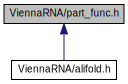
\includegraphics[width=200pt]{part__func_8h__dep__incl}
\end{center}
\end{figure}
\subsection*{Functions}
\begin{DoxyCompactItemize}
\item 
float \hyperlink{group__pf__fold_ga29e256d688ad221b78d37f427e0e99bc}{vrna\+\_\+pf} (\hyperlink{group__fold__compound_ga1b0cef17fd40466cef5968eaeeff6166}{vrna\+\_\+fold\+\_\+compound\+\_\+t} $\ast$vc, char $\ast$structure)
\begin{DoxyCompactList}\small\item\em Compute the partition function $Q$ for a given R\+N\+A sequence, or sequence alignment. \end{DoxyCompactList}\item 
float \hyperlink{group__pf__fold_ga59935ba485ac90f0efb5a38e2962d879}{vrna\+\_\+pf\+\_\+fold} (const char $\ast$seq, char $\ast$structure, \hyperlink{group__data__structures_ga8e4eb5e1bfc95776559575beb359af87}{vrna\+\_\+plist\+\_\+t} $\ast$$\ast$pl)
\begin{DoxyCompactList}\small\item\em Compute Partition function $Q$ (and base pair probabilities) for an R\+N\+A sequence using a comparative method. \end{DoxyCompactList}\item 
float \hyperlink{group__pf__fold_ga6dc133fce577fc0370986f3a3301cd10}{vrna\+\_\+pf\+\_\+circfold} (const char $\ast$seq, char $\ast$structure, \hyperlink{group__data__structures_ga8e4eb5e1bfc95776559575beb359af87}{vrna\+\_\+plist\+\_\+t} $\ast$$\ast$pl)
\begin{DoxyCompactList}\small\item\em Compute Partition function $Q$ (and base pair probabilities) for a circular R\+N\+A sequences using a comparative method. \end{DoxyCompactList}\item 
int \hyperlink{part__func_8h_ad2b3594f0b50b68029e0f54fdce59313}{vrna\+\_\+pf\+\_\+float\+\_\+precision} (void)
\begin{DoxyCompactList}\small\item\em Find out whether partition function computations are using single precision floating points. \end{DoxyCompactList}\item 
double \hyperlink{group__pf__fold_gad3f0c240512e6d43e2e4d4c2076021f5}{vrna\+\_\+mean\+\_\+bp\+\_\+distance\+\_\+pr} (int length, \hyperlink{group__data__structures_ga31125aeace516926bf7f251f759b6126}{F\+L\+T\+\_\+\+O\+R\+\_\+\+D\+B\+L} $\ast$\hyperlink{fold__vars_8h_ac98ec419070aee6831b44e5c700f090f}{pr})
\begin{DoxyCompactList}\small\item\em Get the mean base pair distance in the thermodynamic ensemble from a probability matrix. \end{DoxyCompactList}\item 
double \hyperlink{group__pf__fold_gaa6b8983b559b9ef4b2e1b31113ea317b}{vrna\+\_\+mean\+\_\+bp\+\_\+distance} (\hyperlink{group__fold__compound_ga1b0cef17fd40466cef5968eaeeff6166}{vrna\+\_\+fold\+\_\+compound\+\_\+t} $\ast$vc)
\begin{DoxyCompactList}\small\item\em Get the mean base pair distance in the thermodynamic ensemble. \end{DoxyCompactList}\item 
\hyperlink{group__data__structures_ga8e4eb5e1bfc95776559575beb359af87}{vrna\+\_\+plist\+\_\+t} $\ast$ \hyperlink{group__pf__fold_ga26e3cc2eb127a35625572e9275c24ee4}{vrna\+\_\+stack\+\_\+prob} (\hyperlink{group__fold__compound_ga1b0cef17fd40466cef5968eaeeff6166}{vrna\+\_\+fold\+\_\+compound\+\_\+t} $\ast$vc, double cutoff)
\begin{DoxyCompactList}\small\item\em Compute stacking probabilities. \end{DoxyCompactList}\item 
float \hyperlink{group__pf__fold_gac4f95bee734b2563a3d6e9932117ebdf}{pf\+\_\+fold\+\_\+par} (const char $\ast$sequence, char $\ast$structure, \hyperlink{group__energy__parameters_ga01d8b92fe734df8d79a6169482c7d8d8}{vrna\+\_\+exp\+\_\+param\+\_\+t} $\ast$parameters, int calculate\+\_\+bppm, int is\+\_\+constrained, int is\+\_\+circular)
\begin{DoxyCompactList}\small\item\em Compute the partition function $Q$ for a given R\+N\+A sequence. \end{DoxyCompactList}\item 
float \hyperlink{group__pf__fold_gadc3db3d98742427e7001a7fd36ef28c2}{pf\+\_\+fold} (const char $\ast$sequence, char $\ast$structure)
\begin{DoxyCompactList}\small\item\em Compute the partition function $Q$ of an R\+N\+A sequence. \end{DoxyCompactList}\item 
float \hyperlink{group__pf__fold_ga819ce5fca8984004ac81c4a3b04cb735}{pf\+\_\+circ\+\_\+fold} (const char $\ast$sequence, char $\ast$structure)
\begin{DoxyCompactList}\small\item\em Compute the partition function of a circular R\+N\+A sequence. \end{DoxyCompactList}\item 
char $\ast$ \hyperlink{group__subopt__stochbt_gac03ca6db186bb3bf0a2a326d7fb3ba03}{pbacktrack} (char $\ast$sequence)
\begin{DoxyCompactList}\small\item\em Sample a secondary structure from the Boltzmann ensemble according its probability. \end{DoxyCompactList}\item 
char $\ast$ \hyperlink{group__subopt__stochbt_ga00474051204ac9ad576b3e45174d03ff}{pbacktrack\+\_\+circ} (char $\ast$sequence)
\begin{DoxyCompactList}\small\item\em Sample a secondary structure of a circular R\+N\+A from the Boltzmann ensemble according its probability. \end{DoxyCompactList}\item 
void \hyperlink{group__pf__fold_gae73db3f49a94f0f72e067ecd12681dbd}{free\+\_\+pf\+\_\+arrays} (void)
\begin{DoxyCompactList}\small\item\em Free arrays for the partition function recursions. \end{DoxyCompactList}\item 
void \hyperlink{group__pf__fold_ga384e927890f9c034ff09fa66da102d28}{update\+\_\+pf\+\_\+params} (int length)
\begin{DoxyCompactList}\small\item\em Recalculate energy parameters. \end{DoxyCompactList}\item 
void \hyperlink{group__pf__fold_gaafe2d1b21f5418b123b088aa395e827d}{update\+\_\+pf\+\_\+params\+\_\+par} (int length, \hyperlink{group__energy__parameters_ga01d8b92fe734df8d79a6169482c7d8d8}{vrna\+\_\+exp\+\_\+param\+\_\+t} $\ast$parameters)
\begin{DoxyCompactList}\small\item\em Recalculate energy parameters. \end{DoxyCompactList}\item 
\hyperlink{group__data__structures_ga31125aeace516926bf7f251f759b6126}{F\+L\+T\+\_\+\+O\+R\+\_\+\+D\+B\+L} $\ast$ \hyperlink{group__pf__fold_gac5ac7ee281aae1c5cc5898a841178073}{export\+\_\+bppm} (void)
\begin{DoxyCompactList}\small\item\em Get a pointer to the base pair probability array

Accessing the base pair probabilities for a pair (i,j) is achieved by. \end{DoxyCompactList}\item 
int \hyperlink{group__pf__fold_ga42faebdfce6f070c5f89adfc8427525c}{get\+\_\+pf\+\_\+arrays} (short $\ast$$\ast$S\+\_\+p, short $\ast$$\ast$S1\+\_\+p, char $\ast$$\ast$ptype\+\_\+p, \hyperlink{group__data__structures_ga31125aeace516926bf7f251f759b6126}{F\+L\+T\+\_\+\+O\+R\+\_\+\+D\+B\+L} $\ast$$\ast$qb\+\_\+p, \hyperlink{group__data__structures_ga31125aeace516926bf7f251f759b6126}{F\+L\+T\+\_\+\+O\+R\+\_\+\+D\+B\+L} $\ast$$\ast$qm\+\_\+p, \hyperlink{group__data__structures_ga31125aeace516926bf7f251f759b6126}{F\+L\+T\+\_\+\+O\+R\+\_\+\+D\+B\+L} $\ast$$\ast$q1k\+\_\+p, \hyperlink{group__data__structures_ga31125aeace516926bf7f251f759b6126}{F\+L\+T\+\_\+\+O\+R\+\_\+\+D\+B\+L} $\ast$$\ast$qln\+\_\+p)
\begin{DoxyCompactList}\small\item\em Get the pointers to (almost) all relavant computation arrays used in partition function computation. \end{DoxyCompactList}\item 
\hypertarget{part__func_8h_a189e2a1ec6cc32c53ea72f7543b0441e}{}double \hyperlink{part__func_8h_a189e2a1ec6cc32c53ea72f7543b0441e}{get\+\_\+subseq\+\_\+\+F} (int i, int j)\label{part__func_8h_a189e2a1ec6cc32c53ea72f7543b0441e}

\begin{DoxyCompactList}\small\item\em Get the free energy of a subsequence from the q\mbox{[}\mbox{]} array. \end{DoxyCompactList}\item 
double \hyperlink{group__pf__fold_ga79cbc375af65f11609feb6b055269e7d}{mean\+\_\+bp\+\_\+distance} (int length)
\begin{DoxyCompactList}\small\item\em Get the mean base pair distance of the last partition function computation. \end{DoxyCompactList}\item 
double \hyperlink{group__pf__fold_gad5ba36cef8d01cf4244cc09b9bf1ce1d}{mean\+\_\+bp\+\_\+distance\+\_\+pr} (int length, \hyperlink{group__data__structures_ga31125aeace516926bf7f251f759b6126}{F\+L\+T\+\_\+\+O\+R\+\_\+\+D\+B\+L} $\ast$\hyperlink{fold__vars_8h_ac98ec419070aee6831b44e5c700f090f}{pr})
\begin{DoxyCompactList}\small\item\em Get the mean base pair distance in the thermodynamic ensemble. \end{DoxyCompactList}\item 
\hyperlink{group__data__structures_ga8e4eb5e1bfc95776559575beb359af87}{vrna\+\_\+plist\+\_\+t} $\ast$ \hyperlink{part__func_8h_ae856dd7a8d75c471c07153882bf1db48}{stack\+Prob} (double cutoff)
\begin{DoxyCompactList}\small\item\em Get the probability of stacks. \end{DoxyCompactList}\item 
void \hyperlink{part__func_8h_a15176e23eceeff8c7d14eabcfec8a2af}{init\+\_\+pf\+\_\+fold} (int length)
\begin{DoxyCompactList}\small\item\em Allocate space for \hyperlink{group__pf__fold_gadc3db3d98742427e7001a7fd36ef28c2}{pf\+\_\+fold()} \end{DoxyCompactList}\item 
char $\ast$ \hyperlink{part__func_8h_ae89a63bd83e75a80b2ba36d20b31ce81}{centroid} (int length, double $\ast$dist)
\item 
char $\ast$ \hyperlink{part__func_8h_a4e99e951dfdc006fe56c3a59374378ed}{get\+\_\+centroid\+\_\+struct\+\_\+gquad\+\_\+pr} (int length, double $\ast$dist)
\item 
double \hyperlink{part__func_8h_ae9556ba7ded44fe2321b6f67c3fc02a3}{mean\+\_\+bp\+\_\+dist} (int length)
\item 
double \hyperlink{part__func_8h_a68ba6f3a48e08ca131ab54621ce3a2d7}{exp\+Loop\+Energy} (int u1, int u2, int type, int type2, short si1, short sj1, short sp1, short sq1)
\item 
double \hyperlink{part__func_8h_a7b6ab474cc80accc48010ccfcc59f96b}{exp\+Hairpin\+Energy} (int u, int type, short si1, short sj1, const char $\ast$string)
\end{DoxyCompactItemize}
\subsection*{Variables}
\begin{DoxyCompactItemize}
\item 
int \hyperlink{group__subopt__stochbt_gacd79b1a570e6ad9be24cb11fe8cae30a}{st\+\_\+back}
\begin{DoxyCompactList}\small\item\em Flag indicating that auxilary arrays are needed throughout the computations. This is essential for stochastic backtracking. \end{DoxyCompactList}\end{DoxyCompactItemize}


\subsection{Detailed Description}
Partition function of single R\+N\+A sequences. 

This file includes (almost) all function declarations within the {\bfseries R\+N\+Alib} that are related to Partion function folding... 

\subsection{Function Documentation}
\hypertarget{part__func_8h_ad2b3594f0b50b68029e0f54fdce59313}{}\index{part\+\_\+func.\+h@{part\+\_\+func.\+h}!vrna\+\_\+pf\+\_\+float\+\_\+precision@{vrna\+\_\+pf\+\_\+float\+\_\+precision}}
\index{vrna\+\_\+pf\+\_\+float\+\_\+precision@{vrna\+\_\+pf\+\_\+float\+\_\+precision}!part\+\_\+func.\+h@{part\+\_\+func.\+h}}
\subsubsection[{vrna\+\_\+pf\+\_\+float\+\_\+precision}]{\setlength{\rightskip}{0pt plus 5cm}int vrna\+\_\+pf\+\_\+float\+\_\+precision (
\begin{DoxyParamCaption}
\item[{void}]{}
\end{DoxyParamCaption}
)}\label{part__func_8h_ad2b3594f0b50b68029e0f54fdce59313}


Find out whether partition function computations are using single precision floating points. 

\begin{DoxySeeAlso}{See also}
\hyperlink{group__data__structures_ga31125aeace516926bf7f251f759b6126}{F\+L\+T\+\_\+\+O\+R\+\_\+\+D\+B\+L} 
\end{DoxySeeAlso}
\begin{DoxyReturn}{Returns}
1 if single precision is used, 0 otherwise 
\end{DoxyReturn}
\hypertarget{part__func_8h_ae856dd7a8d75c471c07153882bf1db48}{}\index{part\+\_\+func.\+h@{part\+\_\+func.\+h}!stack\+Prob@{stack\+Prob}}
\index{stack\+Prob@{stack\+Prob}!part\+\_\+func.\+h@{part\+\_\+func.\+h}}
\subsubsection[{stack\+Prob}]{\setlength{\rightskip}{0pt plus 5cm}{\bf vrna\+\_\+plist\+\_\+t}$\ast$ stack\+Prob (
\begin{DoxyParamCaption}
\item[{double}]{cutoff}
\end{DoxyParamCaption}
)}\label{part__func_8h_ae856dd7a8d75c471c07153882bf1db48}


Get the probability of stacks. 

\begin{DoxyRefDesc}{Deprecated}
\item[\hyperlink{deprecated__deprecated000102}{Deprecated}]Use \hyperlink{group__pf__fold_ga26e3cc2eb127a35625572e9275c24ee4}{vrna\+\_\+stack\+\_\+prob()} instead! \end{DoxyRefDesc}
\hypertarget{part__func_8h_a15176e23eceeff8c7d14eabcfec8a2af}{}\index{part\+\_\+func.\+h@{part\+\_\+func.\+h}!init\+\_\+pf\+\_\+fold@{init\+\_\+pf\+\_\+fold}}
\index{init\+\_\+pf\+\_\+fold@{init\+\_\+pf\+\_\+fold}!part\+\_\+func.\+h@{part\+\_\+func.\+h}}
\subsubsection[{init\+\_\+pf\+\_\+fold}]{\setlength{\rightskip}{0pt plus 5cm}void init\+\_\+pf\+\_\+fold (
\begin{DoxyParamCaption}
\item[{int}]{length}
\end{DoxyParamCaption}
)}\label{part__func_8h_a15176e23eceeff8c7d14eabcfec8a2af}


Allocate space for \hyperlink{group__pf__fold_gadc3db3d98742427e7001a7fd36ef28c2}{pf\+\_\+fold()} 

\begin{DoxyRefDesc}{Deprecated}
\item[\hyperlink{deprecated__deprecated000103}{Deprecated}]This function is obsolete and will be removed soon! \end{DoxyRefDesc}
\hypertarget{part__func_8h_ae89a63bd83e75a80b2ba36d20b31ce81}{}\index{part\+\_\+func.\+h@{part\+\_\+func.\+h}!centroid@{centroid}}
\index{centroid@{centroid}!part\+\_\+func.\+h@{part\+\_\+func.\+h}}
\subsubsection[{centroid}]{\setlength{\rightskip}{0pt plus 5cm}char$\ast$ centroid (
\begin{DoxyParamCaption}
\item[{int}]{length, }
\item[{double $\ast$}]{dist}
\end{DoxyParamCaption}
)}\label{part__func_8h_ae89a63bd83e75a80b2ba36d20b31ce81}
\begin{DoxyRefDesc}{Deprecated}
\item[\hyperlink{deprecated__deprecated000104}{Deprecated}]This function is deprecated and should not be used anymore as it is not threadsafe! \begin{DoxySeeAlso}{See also}
\hyperlink{centroid_8h_a8f387bf1583fb5eaf5f4ffd78493e43e}{get\+\_\+centroid\+\_\+struct\+\_\+pl()}, \hyperlink{centroid_8h_ac92486ce514677256f4a832dc518759c}{get\+\_\+centroid\+\_\+struct\+\_\+pr()} 
\end{DoxySeeAlso}
\end{DoxyRefDesc}
\hypertarget{part__func_8h_a4e99e951dfdc006fe56c3a59374378ed}{}\index{part\+\_\+func.\+h@{part\+\_\+func.\+h}!get\+\_\+centroid\+\_\+struct\+\_\+gquad\+\_\+pr@{get\+\_\+centroid\+\_\+struct\+\_\+gquad\+\_\+pr}}
\index{get\+\_\+centroid\+\_\+struct\+\_\+gquad\+\_\+pr@{get\+\_\+centroid\+\_\+struct\+\_\+gquad\+\_\+pr}!part\+\_\+func.\+h@{part\+\_\+func.\+h}}
\subsubsection[{get\+\_\+centroid\+\_\+struct\+\_\+gquad\+\_\+pr}]{\setlength{\rightskip}{0pt plus 5cm}char$\ast$ get\+\_\+centroid\+\_\+struct\+\_\+gquad\+\_\+pr (
\begin{DoxyParamCaption}
\item[{int}]{length, }
\item[{double $\ast$}]{dist}
\end{DoxyParamCaption}
)}\label{part__func_8h_a4e99e951dfdc006fe56c3a59374378ed}
\begin{DoxyRefDesc}{Deprecated}
\item[\hyperlink{deprecated__deprecated000105}{Deprecated}]This function is deprecated and should not be used anymore as it is not threadsafe! \begin{DoxySeeAlso}{See also}
\hyperlink{group__centroid__fold_ga0e64bb67e51963dc71cbd4d30b80a018}{vrna\+\_\+centroid()}, \hyperlink{group__centroid__fold_ga98193ede06778a9ea966cc8fc43d0804}{vrna\+\_\+centroid\+\_\+from\+\_\+probs()}, \hyperlink{group__centroid__fold_ga70525a53b879c1427f9ea546c96fa1c5}{vrna\+\_\+centroid\+\_\+from\+\_\+plist()} 
\end{DoxySeeAlso}
\end{DoxyRefDesc}
\hypertarget{part__func_8h_ae9556ba7ded44fe2321b6f67c3fc02a3}{}\index{part\+\_\+func.\+h@{part\+\_\+func.\+h}!mean\+\_\+bp\+\_\+dist@{mean\+\_\+bp\+\_\+dist}}
\index{mean\+\_\+bp\+\_\+dist@{mean\+\_\+bp\+\_\+dist}!part\+\_\+func.\+h@{part\+\_\+func.\+h}}
\subsubsection[{mean\+\_\+bp\+\_\+dist}]{\setlength{\rightskip}{0pt plus 5cm}double mean\+\_\+bp\+\_\+dist (
\begin{DoxyParamCaption}
\item[{int}]{length}
\end{DoxyParamCaption}
)}\label{part__func_8h_ae9556ba7ded44fe2321b6f67c3fc02a3}
get the mean pair distance of ensemble

\begin{DoxyRefDesc}{Deprecated}
\item[\hyperlink{deprecated__deprecated000106}{Deprecated}]This function is not threadsafe and should not be used anymore. Use \hyperlink{group__pf__fold_ga79cbc375af65f11609feb6b055269e7d}{mean\+\_\+bp\+\_\+distance()} instead! \end{DoxyRefDesc}
\hypertarget{part__func_8h_a68ba6f3a48e08ca131ab54621ce3a2d7}{}\index{part\+\_\+func.\+h@{part\+\_\+func.\+h}!exp\+Loop\+Energy@{exp\+Loop\+Energy}}
\index{exp\+Loop\+Energy@{exp\+Loop\+Energy}!part\+\_\+func.\+h@{part\+\_\+func.\+h}}
\subsubsection[{exp\+Loop\+Energy}]{\setlength{\rightskip}{0pt plus 5cm}double exp\+Loop\+Energy (
\begin{DoxyParamCaption}
\item[{int}]{u1, }
\item[{int}]{u2, }
\item[{int}]{type, }
\item[{int}]{type2, }
\item[{short}]{si1, }
\item[{short}]{sj1, }
\item[{short}]{sp1, }
\item[{short}]{sq1}
\end{DoxyParamCaption}
)}\label{part__func_8h_a68ba6f3a48e08ca131ab54621ce3a2d7}
\begin{DoxyRefDesc}{Deprecated}
\item[\hyperlink{deprecated__deprecated000107}{Deprecated}]Use \hyperlink{group__loops_ga34e8abb9e1b54fab38524fb20214a43e}{exp\+\_\+\+E\+\_\+\+Int\+Loop()} from \hyperlink{loop__energies_8h}{loop\+\_\+energies.\+h} instead \end{DoxyRefDesc}
\hypertarget{part__func_8h_a7b6ab474cc80accc48010ccfcc59f96b}{}\index{part\+\_\+func.\+h@{part\+\_\+func.\+h}!exp\+Hairpin\+Energy@{exp\+Hairpin\+Energy}}
\index{exp\+Hairpin\+Energy@{exp\+Hairpin\+Energy}!part\+\_\+func.\+h@{part\+\_\+func.\+h}}
\subsubsection[{exp\+Hairpin\+Energy}]{\setlength{\rightskip}{0pt plus 5cm}double exp\+Hairpin\+Energy (
\begin{DoxyParamCaption}
\item[{int}]{u, }
\item[{int}]{type, }
\item[{short}]{si1, }
\item[{short}]{sj1, }
\item[{const char $\ast$}]{string}
\end{DoxyParamCaption}
)}\label{part__func_8h_a7b6ab474cc80accc48010ccfcc59f96b}
\begin{DoxyRefDesc}{Deprecated}
\item[\hyperlink{deprecated__deprecated000108}{Deprecated}]Use \hyperlink{group__loops_ga51fb555974f180b78d76142b2894851c}{exp\+\_\+\+E\+\_\+\+Hairpin()} from \hyperlink{loop__energies_8h}{loop\+\_\+energies.\+h} instead \end{DoxyRefDesc}

\input{part__func__co_8h}
\input{part__func__up_8h}
\hypertarget{plot__aln_8h}{\section{Vienna\+R\+N\+A/plot\+\_\+aln.h File Reference}
\label{plot__aln_8h}\index{Vienna\+R\+N\+A/plot\+\_\+aln.\+h@{Vienna\+R\+N\+A/plot\+\_\+aln.\+h}}
}


Various functions for plotting Sequence / Structure Alignments.  


This graph shows which files directly or indirectly include this file\+:
\nopagebreak
\begin{figure}[H]
\begin{center}
\leavevmode
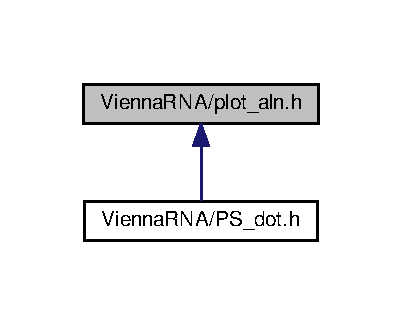
\includegraphics[width=193pt]{plot__aln_8h__dep__incl}
\end{center}
\end{figure}
\subsection*{Functions}
\begin{DoxyCompactItemize}
\item 
\hypertarget{group__plotting__utils_ga821802c3685e37e15182341f6217470d}{int \hyperlink{group__plotting__utils_ga821802c3685e37e15182341f6217470d}{P\+S\+\_\+color\+\_\+aln} (const char $\ast$structure, const char $\ast$filename, const char $\ast$seqs\mbox{[}$\,$\mbox{]}, const char $\ast$names\mbox{[}$\,$\mbox{]})}\label{group__plotting__utils_ga821802c3685e37e15182341f6217470d}

\begin{DoxyCompactList}\small\item\em Produce Post\+Script sequence alignment color-\/annotated by consensus structure. \end{DoxyCompactList}\item 
int \hyperlink{group__plotting__utils_gaab48d4dac655d688abe921389ac2847c}{ali\+P\+S\+\_\+color\+\_\+aln} (const char $\ast$structure, const char $\ast$filename, const char $\ast$seqs\mbox{[}$\,$\mbox{]}, const char $\ast$names\mbox{[}$\,$\mbox{]})
\end{DoxyCompactItemize}


\subsection{Detailed Description}
Various functions for plotting Sequence / Structure Alignments. 


\input{plot__layouts_8h}
\input{plot__structure_8h}
\hypertarget{profiledist_8h}{}\section{Vienna\+R\+N\+A/profiledist.h File Reference}
\label{profiledist_8h}\index{Vienna\+R\+N\+A/profiledist.\+h@{Vienna\+R\+N\+A/profiledist.\+h}}
Include dependency graph for profiledist.\+h\+:
\nopagebreak
\begin{figure}[H]
\begin{center}
\leavevmode
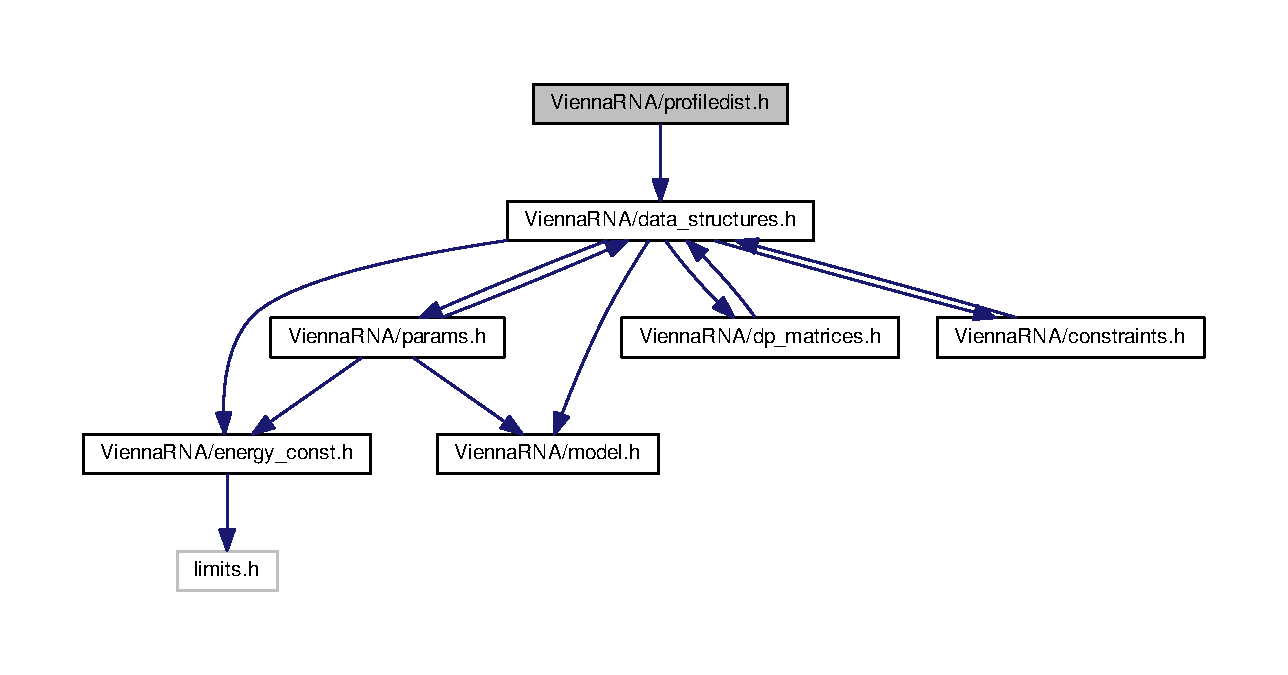
\includegraphics[width=350pt]{profiledist_8h__incl}
\end{center}
\end{figure}
\subsection*{Functions}
\begin{DoxyCompactItemize}
\item 
float \hyperlink{profiledist_8h_abe75e90e00a1e5dd8862944ed53dad5d}{profile\+\_\+edit\+\_\+distance} (const float $\ast$T1, const float $\ast$T2)
\begin{DoxyCompactList}\small\item\em Align the 2 probability profiles T1, T2~\newline
. \end{DoxyCompactList}\item 
float $\ast$ \hyperlink{profiledist_8h_a3dff26e707a2a2e65a0f759caabde6e7}{Make\+\_\+bp\+\_\+profile\+\_\+bppm} (\hyperlink{group__data__structures_ga31125aeace516926bf7f251f759b6126}{F\+L\+T\+\_\+\+O\+R\+\_\+\+D\+B\+L} $\ast$bppm, int length)
\begin{DoxyCompactList}\small\item\em condense pair probability matrix into a vector containing probabilities for unpaired, upstream paired and downstream paired. \end{DoxyCompactList}\item 
\hypertarget{profiledist_8h_a8e0b4fe3698b3502945116ecc0ba6160}{}void \hyperlink{profiledist_8h_a8e0b4fe3698b3502945116ecc0ba6160}{print\+\_\+bppm} (const float $\ast$T)\label{profiledist_8h_a8e0b4fe3698b3502945116ecc0ba6160}

\begin{DoxyCompactList}\small\item\em print string representation of probability profile \end{DoxyCompactList}\item 
void \hyperlink{profiledist_8h_a9b0b84a5a45761bf42d7c835dcdb3b85}{free\+\_\+profile} (float $\ast$T)
\begin{DoxyCompactList}\small\item\em free space allocated in Make\+\_\+bp\+\_\+profile \end{DoxyCompactList}\item 
float $\ast$ \hyperlink{profiledist_8h_a904c7eaf4a2413567c00ac4891749d18}{Make\+\_\+bp\+\_\+profile} (int length)
\end{DoxyCompactItemize}


\subsection{Function Documentation}
\hypertarget{profiledist_8h_abe75e90e00a1e5dd8862944ed53dad5d}{}\index{profiledist.\+h@{profiledist.\+h}!profile\+\_\+edit\+\_\+distance@{profile\+\_\+edit\+\_\+distance}}
\index{profile\+\_\+edit\+\_\+distance@{profile\+\_\+edit\+\_\+distance}!profiledist.\+h@{profiledist.\+h}}
\subsubsection[{profile\+\_\+edit\+\_\+distance}]{\setlength{\rightskip}{0pt plus 5cm}float profile\+\_\+edit\+\_\+distance (
\begin{DoxyParamCaption}
\item[{const float $\ast$}]{T1, }
\item[{const float $\ast$}]{T2}
\end{DoxyParamCaption}
)}\label{profiledist_8h_abe75e90e00a1e5dd8862944ed53dad5d}


Align the 2 probability profiles T1, T2~\newline
. 

This is like a Needleman-\/\+Wunsch alignment, we should really use affine gap-\/costs ala Gotoh \hypertarget{profiledist_8h_a3dff26e707a2a2e65a0f759caabde6e7}{}\index{profiledist.\+h@{profiledist.\+h}!Make\+\_\+bp\+\_\+profile\+\_\+bppm@{Make\+\_\+bp\+\_\+profile\+\_\+bppm}}
\index{Make\+\_\+bp\+\_\+profile\+\_\+bppm@{Make\+\_\+bp\+\_\+profile\+\_\+bppm}!profiledist.\+h@{profiledist.\+h}}
\subsubsection[{Make\+\_\+bp\+\_\+profile\+\_\+bppm}]{\setlength{\rightskip}{0pt plus 5cm}float$\ast$ Make\+\_\+bp\+\_\+profile\+\_\+bppm (
\begin{DoxyParamCaption}
\item[{{\bf F\+L\+T\+\_\+\+O\+R\+\_\+\+D\+B\+L} $\ast$}]{bppm, }
\item[{int}]{length}
\end{DoxyParamCaption}
)}\label{profiledist_8h_a3dff26e707a2a2e65a0f759caabde6e7}


condense pair probability matrix into a vector containing probabilities for unpaired, upstream paired and downstream paired. 

This resulting probability profile is used as input for profile\+\_\+edit\+\_\+distance


\begin{DoxyParams}{Parameters}
{\em bppm} & A pointer to the base pair probability matrix \\
\hline
{\em length} & The length of the sequence \\
\hline
\end{DoxyParams}
\begin{DoxyReturn}{Returns}
The bp profile 
\end{DoxyReturn}
\hypertarget{profiledist_8h_a9b0b84a5a45761bf42d7c835dcdb3b85}{}\index{profiledist.\+h@{profiledist.\+h}!free\+\_\+profile@{free\+\_\+profile}}
\index{free\+\_\+profile@{free\+\_\+profile}!profiledist.\+h@{profiledist.\+h}}
\subsubsection[{free\+\_\+profile}]{\setlength{\rightskip}{0pt plus 5cm}void free\+\_\+profile (
\begin{DoxyParamCaption}
\item[{float $\ast$}]{T}
\end{DoxyParamCaption}
)}\label{profiledist_8h_a9b0b84a5a45761bf42d7c835dcdb3b85}


free space allocated in Make\+\_\+bp\+\_\+profile 

Backward compatibility only. You can just use plain free() \hypertarget{profiledist_8h_a904c7eaf4a2413567c00ac4891749d18}{}\index{profiledist.\+h@{profiledist.\+h}!Make\+\_\+bp\+\_\+profile@{Make\+\_\+bp\+\_\+profile}}
\index{Make\+\_\+bp\+\_\+profile@{Make\+\_\+bp\+\_\+profile}!profiledist.\+h@{profiledist.\+h}}
\subsubsection[{Make\+\_\+bp\+\_\+profile}]{\setlength{\rightskip}{0pt plus 5cm}float$\ast$ Make\+\_\+bp\+\_\+profile (
\begin{DoxyParamCaption}
\item[{int}]{length}
\end{DoxyParamCaption}
)}\label{profiledist_8h_a904c7eaf4a2413567c00ac4891749d18}
\begin{DoxyNote}{Note}
This function is N\+O\+T threadsafe
\end{DoxyNote}
\begin{DoxySeeAlso}{See also}
\hyperlink{profiledist_8h_a3dff26e707a2a2e65a0f759caabde6e7}{Make\+\_\+bp\+\_\+profile\+\_\+bppm()}
\end{DoxySeeAlso}
\begin{DoxyRefDesc}{Deprecated}
\item[\hyperlink{deprecated__deprecated000122}{Deprecated}]This function is deprecated and will be removed soon! See \hyperlink{profiledist_8h_a3dff26e707a2a2e65a0f759caabde6e7}{Make\+\_\+bp\+\_\+profile\+\_\+bppm()} for a replacement\end{DoxyRefDesc}

\hypertarget{PS__dot_8h}{\section{Vienna\+R\+N\+A/\+P\+S\+\_\+dot.h File Reference}
\label{PS__dot_8h}\index{Vienna\+R\+N\+A/\+P\+S\+\_\+dot.\+h@{Vienna\+R\+N\+A/\+P\+S\+\_\+dot.\+h}}
}


Various functions for plotting R\+N\+A secondary structures, dot-\/plots and other visualizations.  


Include dependency graph for P\+S\+\_\+dot.\+h\+:
\nopagebreak
\begin{figure}[H]
\begin{center}
\leavevmode
\includegraphics[width=350pt]{PS__dot_8h__incl}
\end{center}
\end{figure}
\subsection*{Functions}
\begin{DoxyCompactItemize}
\item 
int \hyperlink{group__plotting__utils_ga00ea223b5cf02eb2faae5ff29f0d5e12}{P\+S\+\_\+dot\+\_\+plot\+\_\+list} (char $\ast$seq, char $\ast$filename, \hyperlink{group__data__structures_gab1d8894b43aa84cbc50b862a73785fbc}{plist} $\ast$pl, \hyperlink{group__data__structures_gab1d8894b43aa84cbc50b862a73785fbc}{plist} $\ast$mf, char $\ast$comment)
\begin{DoxyCompactList}\small\item\em Produce a postscript dot-\/plot from two pair lists. \end{DoxyCompactList}\item 
int \hyperlink{group__plotting__utils_ga689a97a7e3b8a2df14728b8204d9d57b}{P\+S\+\_\+dot\+\_\+plot} (char $\ast$string, char $\ast$file)
\begin{DoxyCompactList}\small\item\em Produce postscript dot-\/plot. \end{DoxyCompactList}\end{DoxyCompactItemize}


\subsection{Detailed Description}
Various functions for plotting R\+N\+A secondary structures, dot-\/plots and other visualizations. 


\input{read__epars_8h}
\hypertarget{ribo_8h}{}\section{Vienna\+R\+N\+A/ribo.h File Reference}
\label{ribo_8h}\index{Vienna\+R\+N\+A/ribo.\+h@{Vienna\+R\+N\+A/ribo.\+h}}


Parse Ribo\+Sum Scoring Matrices for Covariance Scoring of Alignments.  


This graph shows which files directly or indirectly include this file\+:
\nopagebreak
\begin{figure}[H]
\begin{center}
\leavevmode
\includegraphics[width=185pt]{ribo_8h__dep__incl}
\end{center}
\end{figure}
\subsection*{Functions}
\begin{DoxyCompactItemize}
\item 
\hypertarget{group__consensus__fold_ga1116aed4b2dab5252cd23946d47d52c3}{}float $\ast$$\ast$ \hyperlink{group__consensus__fold_ga1116aed4b2dab5252cd23946d47d52c3}{get\+\_\+ribosum} (const char $\ast$$\ast$Alseq, int n\+\_\+seq, int length)\label{group__consensus__fold_ga1116aed4b2dab5252cd23946d47d52c3}

\begin{DoxyCompactList}\small\item\em Retrieve a Ribo\+Sum Scoring Matrix for a given Alignment. \end{DoxyCompactList}\item 
\hypertarget{group__file__utils_ga5e125c9586fcd4e2e1559fe76f7289cc}{}float $\ast$$\ast$ \hyperlink{group__file__utils_ga5e125c9586fcd4e2e1559fe76f7289cc}{readribosum} (char $\ast$name)\label{group__file__utils_ga5e125c9586fcd4e2e1559fe76f7289cc}

\begin{DoxyCompactList}\small\item\em Read a Ribo\+Sum or other user-\/defined Scoring Matrix and Store into global Memory. \end{DoxyCompactList}\end{DoxyCompactItemize}


\subsection{Detailed Description}
Parse Ribo\+Sum Scoring Matrices for Covariance Scoring of Alignments. 


\input{RNAstruct_8h}
\input{string__utils_8h}
\hypertarget{stringdist_8h}{\section{Vienna\+R\+N\+A/stringdist.h File Reference}
\label{stringdist_8h}\index{Vienna\+R\+N\+A/stringdist.\+h@{Vienna\+R\+N\+A/stringdist.\+h}}
}


Functions for String Alignment.  


Include dependency graph for stringdist.\+h\+:
\nopagebreak
\begin{figure}[H]
\begin{center}
\leavevmode
\includegraphics[width=199pt]{stringdist_8h__incl}
\end{center}
\end{figure}
\subsection*{Functions}
\begin{DoxyCompactItemize}
\item 
\hyperlink{structswString}{sw\+String} $\ast$ \hyperlink{stringdist_8h_a3125991b3a403b3f89230474deb3f22e}{Make\+\_\+sw\+String} (char $\ast$string)
\begin{DoxyCompactList}\small\item\em Convert a structure into a format suitable for \hyperlink{stringdist_8h_a89e3c335ef17780576d7c0e713830db9}{string\+\_\+edit\+\_\+distance()}. \end{DoxyCompactList}\item 
float \hyperlink{stringdist_8h_a89e3c335ef17780576d7c0e713830db9}{string\+\_\+edit\+\_\+distance} (\hyperlink{structswString}{sw\+String} $\ast$T1, \hyperlink{structswString}{sw\+String} $\ast$T2)
\begin{DoxyCompactList}\small\item\em Calculate the string edit distance of T1 and T2. \end{DoxyCompactList}\end{DoxyCompactItemize}


\subsection{Detailed Description}
Functions for String Alignment. 



\subsection{Function Documentation}
\hypertarget{stringdist_8h_a3125991b3a403b3f89230474deb3f22e}{\index{stringdist.\+h@{stringdist.\+h}!Make\+\_\+sw\+String@{Make\+\_\+sw\+String}}
\index{Make\+\_\+sw\+String@{Make\+\_\+sw\+String}!stringdist.\+h@{stringdist.\+h}}
\subsubsection[{Make\+\_\+sw\+String}]{\setlength{\rightskip}{0pt plus 5cm}{\bf sw\+String}$\ast$ Make\+\_\+sw\+String (
\begin{DoxyParamCaption}
\item[{char $\ast$}]{string}
\end{DoxyParamCaption}
)}}\label{stringdist_8h_a3125991b3a403b3f89230474deb3f22e}


Convert a structure into a format suitable for \hyperlink{stringdist_8h_a89e3c335ef17780576d7c0e713830db9}{string\+\_\+edit\+\_\+distance()}. 


\begin{DoxyParams}{Parameters}
{\em string} & \\
\hline
\end{DoxyParams}
\begin{DoxyReturn}{Returns}

\end{DoxyReturn}
\hypertarget{stringdist_8h_a89e3c335ef17780576d7c0e713830db9}{\index{stringdist.\+h@{stringdist.\+h}!string\+\_\+edit\+\_\+distance@{string\+\_\+edit\+\_\+distance}}
\index{string\+\_\+edit\+\_\+distance@{string\+\_\+edit\+\_\+distance}!stringdist.\+h@{stringdist.\+h}}
\subsubsection[{string\+\_\+edit\+\_\+distance}]{\setlength{\rightskip}{0pt plus 5cm}float string\+\_\+edit\+\_\+distance (
\begin{DoxyParamCaption}
\item[{{\bf sw\+String} $\ast$}]{T1, }
\item[{{\bf sw\+String} $\ast$}]{T2}
\end{DoxyParamCaption}
)}}\label{stringdist_8h_a89e3c335ef17780576d7c0e713830db9}


Calculate the string edit distance of T1 and T2. 


\begin{DoxyParams}{Parameters}
{\em T1} & \\
\hline
{\em T2} & \\
\hline
\end{DoxyParams}
\begin{DoxyReturn}{Returns}

\end{DoxyReturn}

\input{structure__utils_8h}
\hypertarget{subopt_8h}{}\section{Vienna\+R\+N\+A/subopt.h File Reference}
\label{subopt_8h}\index{Vienna\+R\+N\+A/subopt.\+h@{Vienna\+R\+N\+A/subopt.\+h}}


R\+N\+Asubopt and density of states declarations.  


Include dependency graph for subopt.\+h\+:
\nopagebreak
\begin{figure}[H]
\begin{center}
\leavevmode
\includegraphics[width=350pt]{subopt_8h__incl}
\end{center}
\end{figure}
\subsection*{Data Structures}
\begin{DoxyCompactItemize}
\item 
struct \hyperlink{structvrna__subopt__sol__s}{vrna\+\_\+subopt\+\_\+sol\+\_\+s}
\begin{DoxyCompactList}\small\item\em Solution element from subopt.\+c. \end{DoxyCompactList}\end{DoxyCompactItemize}
\subsection*{Macros}
\begin{DoxyCompactItemize}
\item 
\hypertarget{subopt_8h_a5ec740b80afb4906ba4311dbd8ddbd89}{}\#define \hyperlink{subopt_8h_a5ec740b80afb4906ba4311dbd8ddbd89}{M\+A\+X\+D\+O\+S}~1000\label{subopt_8h_a5ec740b80afb4906ba4311dbd8ddbd89}

\begin{DoxyCompactList}\small\item\em Maximum density of states discretization for subopt. \end{DoxyCompactList}\end{DoxyCompactItemize}
\subsection*{Functions}
\begin{DoxyCompactItemize}
\item 
\hyperlink{structvrna__subopt__sol__s}{vrna\+\_\+subopt\+\_\+solution\+\_\+t} $\ast$ \hyperlink{group__subopt__wuchty_ga7988544ae3fc6334c1517cf76e5660aa}{vrna\+\_\+subopt} (\hyperlink{group__fold__compound_ga1b0cef17fd40466cef5968eaeeff6166}{vrna\+\_\+fold\+\_\+compound\+\_\+t} $\ast$vc, int delta, int sorted, F\+I\+L\+E $\ast$fp)
\begin{DoxyCompactList}\small\item\em Returns list of subopt structures or writes to fp. \end{DoxyCompactList}\item 
\hyperlink{structvrna__subopt__sol__s}{vrna\+\_\+subopt\+\_\+solution\+\_\+t} $\ast$ \hyperlink{group__subopt__zuker_gac0df98085abd242c7a6b1c868b3a35c8}{vrna\+\_\+subopt\+\_\+zuker} (\hyperlink{group__fold__compound_ga1b0cef17fd40466cef5968eaeeff6166}{vrna\+\_\+fold\+\_\+compound\+\_\+t} $\ast$vc)
\begin{DoxyCompactList}\small\item\em Compute Zuker type suboptimal structures. \end{DoxyCompactList}\item 
\hyperlink{structvrna__subopt__sol__s}{S\+O\+L\+U\+T\+I\+O\+N} $\ast$ \hyperlink{group__subopt__wuchty_ga700f662506a233e42dd7fda74fafd40e}{subopt} (char $\ast$seq, char $\ast$structure, int delta, F\+I\+L\+E $\ast$fp)
\begin{DoxyCompactList}\small\item\em Returns list of subopt structures or writes to fp. \end{DoxyCompactList}\item 
\hypertarget{group__subopt__wuchty_gaa1e1e7031a948ebcb39a9d58d1e9842c}{}\hyperlink{structvrna__subopt__sol__s}{S\+O\+L\+U\+T\+I\+O\+N} $\ast$ \hyperlink{group__subopt__wuchty_gaa1e1e7031a948ebcb39a9d58d1e9842c}{subopt\+\_\+par} (char $\ast$seq, char $\ast$structure, \hyperlink{group__energy__parameters_ga8a69ca7d787e4fd6079914f5343a1f35}{vrna\+\_\+param\+\_\+t} $\ast$parameters, int delta, int is\+\_\+constrained, int is\+\_\+circular, F\+I\+L\+E $\ast$fp)\label{group__subopt__wuchty_gaa1e1e7031a948ebcb39a9d58d1e9842c}

\begin{DoxyCompactList}\small\item\em Returns list of subopt structures or writes to fp. \end{DoxyCompactList}\item 
\hyperlink{structvrna__subopt__sol__s}{S\+O\+L\+U\+T\+I\+O\+N} $\ast$ \hyperlink{group__subopt__wuchty_ga8634516e4740e0b6c9a46d2bae940340}{subopt\+\_\+circ} (char $\ast$seq, char $\ast$sequence, int delta, F\+I\+L\+E $\ast$fp)
\begin{DoxyCompactList}\small\item\em Returns list of circular subopt structures or writes to fp. \end{DoxyCompactList}\item 
\hyperlink{structvrna__subopt__sol__s}{S\+O\+L\+U\+T\+I\+O\+N} $\ast$ \hyperlink{group__subopt__zuker_ga0d5104e3ecf119d8eabd40aa5fe47f90}{zukersubopt} (const char $\ast$string)
\begin{DoxyCompactList}\small\item\em Compute Zuker type suboptimal structures. \end{DoxyCompactList}\item 
\hyperlink{structvrna__subopt__sol__s}{S\+O\+L\+U\+T\+I\+O\+N} $\ast$ \hyperlink{group__subopt__zuker_gab6d0ea8cc1d02f6dd831ca81043c9eb8}{zukersubopt\+\_\+par} (const char $\ast$string, \hyperlink{group__energy__parameters_ga8a69ca7d787e4fd6079914f5343a1f35}{vrna\+\_\+param\+\_\+t} $\ast$parameters)
\begin{DoxyCompactList}\small\item\em Compute Zuker type suboptimal structures. \end{DoxyCompactList}\end{DoxyCompactItemize}
\subsection*{Variables}
\begin{DoxyCompactItemize}
\item 
\hypertarget{group__subopt__wuchty_ga5e57d914bcb5feeecdf520e25313fcfe}{}double \hyperlink{group__subopt__wuchty_ga5e57d914bcb5feeecdf520e25313fcfe}{print\+\_\+energy}\label{group__subopt__wuchty_ga5e57d914bcb5feeecdf520e25313fcfe}

\begin{DoxyCompactList}\small\item\em printing threshold for use with log\+M\+L \end{DoxyCompactList}\item 
\hypertarget{group__subopt__wuchty_ga873cf8ed69e0437f8efa8b1fec854a0e}{}int \hyperlink{group__subopt__wuchty_ga873cf8ed69e0437f8efa8b1fec854a0e}{subopt\+\_\+sorted}\label{group__subopt__wuchty_ga873cf8ed69e0437f8efa8b1fec854a0e}

\begin{DoxyCompactList}\small\item\em Sort output by energy. \end{DoxyCompactList}\item 
int \hyperlink{group__dos_ga937634a76b46a22530a74906f1957a9e}{density\+\_\+of\+\_\+states} \mbox{[}\hyperlink{subopt_8h_a5ec740b80afb4906ba4311dbd8ddbd89}{M\+A\+X\+D\+O\+S}+1\mbox{]}
\begin{DoxyCompactList}\small\item\em The Density of States. \end{DoxyCompactList}\end{DoxyCompactItemize}


\subsection{Detailed Description}
R\+N\+Asubopt and density of states declarations. 


\hypertarget{treedist_8h}{}\section{Vienna\+R\+N\+A/treedist.h File Reference}
\label{treedist_8h}\index{Vienna\+R\+N\+A/treedist.\+h@{Vienna\+R\+N\+A/treedist.\+h}}


Functions for \hyperlink{structTree}{Tree} Edit Distances.  


Include dependency graph for treedist.\+h\+:
\nopagebreak
\begin{figure}[H]
\begin{center}
\leavevmode
\includegraphics[width=199pt]{treedist_8h__incl}
\end{center}
\end{figure}
\subsection*{Functions}
\begin{DoxyCompactItemize}
\item 
\hyperlink{structTree}{Tree} $\ast$ \hyperlink{treedist_8h_a08fe4d5afd385dce593b86eaf010c6e3}{make\+\_\+tree} (char $\ast$struc)
\begin{DoxyCompactList}\small\item\em Constructs a \hyperlink{structTree}{Tree} ( essentially the postorder list ) of the structure \textquotesingle{}struc\textquotesingle{}, for use in \hyperlink{treedist_8h_a3b21f1925f7071f46d93431a835217bb}{tree\+\_\+edit\+\_\+distance()}. \end{DoxyCompactList}\item 
float \hyperlink{treedist_8h_a3b21f1925f7071f46d93431a835217bb}{tree\+\_\+edit\+\_\+distance} (\hyperlink{structTree}{Tree} $\ast$T1, \hyperlink{structTree}{Tree} $\ast$T2)
\begin{DoxyCompactList}\small\item\em Calculates the edit distance of the two trees. \end{DoxyCompactList}\item 
\hypertarget{treedist_8h_a21ad4de3ba4055aeef08b28c9ad48894}{}void \hyperlink{treedist_8h_a21ad4de3ba4055aeef08b28c9ad48894}{print\+\_\+tree} (\hyperlink{structTree}{Tree} $\ast$t)\label{treedist_8h_a21ad4de3ba4055aeef08b28c9ad48894}

\begin{DoxyCompactList}\small\item\em Print a tree (mainly for debugging) \end{DoxyCompactList}\item 
void \hyperlink{treedist_8h_acbc1cb9bce582ea945e4a467c76a57aa}{free\+\_\+tree} (\hyperlink{structTree}{Tree} $\ast$t)
\begin{DoxyCompactList}\small\item\em Free the memory allocated for \hyperlink{structTree}{Tree} t. \end{DoxyCompactList}\end{DoxyCompactItemize}


\subsection{Detailed Description}
Functions for \hyperlink{structTree}{Tree} Edit Distances. 



\subsection{Function Documentation}
\hypertarget{treedist_8h_a08fe4d5afd385dce593b86eaf010c6e3}{}\index{treedist.\+h@{treedist.\+h}!make\+\_\+tree@{make\+\_\+tree}}
\index{make\+\_\+tree@{make\+\_\+tree}!treedist.\+h@{treedist.\+h}}
\subsubsection[{make\+\_\+tree}]{\setlength{\rightskip}{0pt plus 5cm}{\bf Tree}$\ast$ make\+\_\+tree (
\begin{DoxyParamCaption}
\item[{char $\ast$}]{struc}
\end{DoxyParamCaption}
)}\label{treedist_8h_a08fe4d5afd385dce593b86eaf010c6e3}


Constructs a \hyperlink{structTree}{Tree} ( essentially the postorder list ) of the structure \textquotesingle{}struc\textquotesingle{}, for use in \hyperlink{treedist_8h_a3b21f1925f7071f46d93431a835217bb}{tree\+\_\+edit\+\_\+distance()}. 


\begin{DoxyParams}{Parameters}
{\em struc} & may be any rooted structure representation. \\
\hline
\end{DoxyParams}
\begin{DoxyReturn}{Returns}

\end{DoxyReturn}
\hypertarget{treedist_8h_a3b21f1925f7071f46d93431a835217bb}{}\index{treedist.\+h@{treedist.\+h}!tree\+\_\+edit\+\_\+distance@{tree\+\_\+edit\+\_\+distance}}
\index{tree\+\_\+edit\+\_\+distance@{tree\+\_\+edit\+\_\+distance}!treedist.\+h@{treedist.\+h}}
\subsubsection[{tree\+\_\+edit\+\_\+distance}]{\setlength{\rightskip}{0pt plus 5cm}float tree\+\_\+edit\+\_\+distance (
\begin{DoxyParamCaption}
\item[{{\bf Tree} $\ast$}]{T1, }
\item[{{\bf Tree} $\ast$}]{T2}
\end{DoxyParamCaption}
)}\label{treedist_8h_a3b21f1925f7071f46d93431a835217bb}


Calculates the edit distance of the two trees. 


\begin{DoxyParams}{Parameters}
{\em T1} & \\
\hline
{\em T2} & \\
\hline
\end{DoxyParams}
\begin{DoxyReturn}{Returns}

\end{DoxyReturn}
\hypertarget{treedist_8h_acbc1cb9bce582ea945e4a467c76a57aa}{}\index{treedist.\+h@{treedist.\+h}!free\+\_\+tree@{free\+\_\+tree}}
\index{free\+\_\+tree@{free\+\_\+tree}!treedist.\+h@{treedist.\+h}}
\subsubsection[{free\+\_\+tree}]{\setlength{\rightskip}{0pt plus 5cm}void free\+\_\+tree (
\begin{DoxyParamCaption}
\item[{{\bf Tree} $\ast$}]{t}
\end{DoxyParamCaption}
)}\label{treedist_8h_acbc1cb9bce582ea945e4a467c76a57aa}


Free the memory allocated for \hyperlink{structTree}{Tree} t. 


\begin{DoxyParams}{Parameters}
{\em t} & \\
\hline
\end{DoxyParams}

\input{utils_8h}
%--- End generated contents ---

% Bibliography
\newpage
\phantomsection
\addcontentsline{toc}{chapter}{Bibliography}
\bibliographystyle{plain}
\bibliography{bibTmpFile_1}

% Index
\newpage
\phantomsection
\addcontentsline{toc}{chapter}{Index}
\printindex

\end{document}
